\documentclass%
[handout]%
{beamer}

\mode<presentation>
{
\useinnertheme{rounded}
\useoutertheme{infolines}
\usecolortheme{orchid}
\usecolortheme{whale}
}
%\setbeamertemplate{footline}{%
%  \raisebox{5pt}{\makebox[\paperwidth]{\hfill\makebox[10pt]{\scriptsize\insertframenumber}}}}

\usepackage[english]{babel}
\usepackage[latin1]{inputenc}
\usepackage{times}

\usepackage{ifthen}
\usepackage{amsmath}
\usepackage{amssymb}
\usepackage{cancel}
\usepackage{comment}
\usepackage{multirow}
\usepackage{psfrag}
\usepackage{rotating}
\usepackage{fp}
\usepackage{calc}
\usepackage{bm}
\usepackage[all,cmtip]{xy}
\RequirePackage{xstring}

%%%%%%%%%%%%%%%%%%%%%%%%%%%%%%%%%%%%%%%%%%
%
% List of commands in this document
%
%
% \logdiffbaseandexp
% \logdifftwouponedown
% \productrulefofx
% \quotientruley
% \limitradical  (broken)
% \limitsub
% \chainruley
% \chainrulefofx
% \chainruleStyleOne
% \chainruleStyleTwo
% \chainruleStyleThree
% \infinitelimit
% \limitfactor
% \newtonsmethod
% \constantmultiple
% \chainruletwice
% \youWillNotBeTested
% \optionalDisplay  %Dummy command needed for compatibility with Calculus notes.
% \Arcsin
% \Arccos
% \Arctan
% \Arccot
% \diff
%%%%%%%%%%%%%%%%%%%%%%%%%%%%%%%%%%%%%%%%%%

\newcommand{\diff}{{\normalfont \text{d}}}
\newtheorem{question}{Question}
\newtheorem{observation}{Observation}
\newtheorem{proposition}{Proposition}
\newtheorem{remark}{Remark}
\newcommand{\youWillNotBeTested}{\begin{frame}You will not be tested on the material in the following slide.\end{frame}}
\DeclareMathOperator{\Vol}{Vol}

\DeclareMathOperator{\Arcsin}{\sin^{-1}}
\DeclareMathOperator{\Arccos}{\cos^{-1}}
\DeclareMathOperator{\Arctan}{\tan^{-1}}
\DeclareMathOperator{\Arccot}{{\cot^{-1}}}
\DeclareMathOperator{\Arcsec}{{\sec^{-1}}}
\DeclareMathOperator{\Arccsc}{{\csc^{-1}}}
\DeclareMathOperator{\maclaurin}{{\normalfont{Mc}}}
\newcommand{\taylor}{{\normalfont{T}}}

\newcommand{\optionalDisplay}[1]{#1}
\renewcommand{\Im}{\mathrm{Im}}
\renewcommand{\Re}{\mathrm{Re}}

%\DeclareMathOperator{\Re}{Re}
%\DeclareMathOperator{\Im}{Im}
\newcommand{\fcv}[1]{{\bf #1}} %this command stands for freecalc Vector
\DeclareMathOperator{\curl}{\fcv{curl}}
\DeclareMathOperator{\divg}{div}
\DeclareMathOperator{\proj}{\fcv{proj}}
\DeclareMathOperator{\orth}{\fcv{orth}}
\DeclareMathOperator{\grad}{\fcv{grad}}
\newcommand{\RR}{{\mathbb{R}}}
\newcommand{\cR}{{\mathcal{R}}}
\newcommand{\cD}{{\mathcal{D}}}
\newcommand{\cP}{{\mathcal{P}}}
\newcommand{\fcUncoverAlert}[2]{\uncover<#1->{\alert<#1>{#2}}}
\newcommand{\alertNoH}[2]{\alert<handout:0|#1>{#2}}
\newcommand{\fcAnswerNoH}[2]{
\FPeval{\fcResult}{clip(#1-1)}
\uncover<handout:0|\fcResult>{\alert<handout:0|\fcResult>{\textbf{?} }} \uncover<handout:0| #1->{\alert<handout:0|#1>{\!\!\!#2}}
}
\newcommand{\fcAnswer}[2]{
\FPeval{\fcResult}{clip(#1-1)}
\uncover<handout:0|\fcResult>{\alertNoH{\fcResult}{\textbf{?} }} \uncover<#1->{\alertNoH{#1}{\!\!\!#2}}
}
\newcommand{\fcAnswerUncover}[3]{
\FPeval{\fcResult}{clip(#2-1)}
\uncover<handout:0|#1-\fcResult>{\alertNoH{\fcResult}{\textbf{?}}} \uncover<#2->{\alertNoH{#2}{\!\!\!#3}}
}
\newcommand{\fcAnswerUncoverNoH}[3]{
\FPeval{\fcResult}{clip(#2-1)}
\uncover<handout:0|#1-\fcResult>{\alertNoH{\fcResult}{\textbf{?}}} \uncover<handout:0|#2->{\alertNoH{#2}{\!\!\!#3}}
}

\newcommand{\fcQuestion}[2]{%
\FPeval{\fcResult}{clip(#1+1)}%
\uncover<#1->{\alertNoH{ #1,\fcResult}{#2}}%
}
\newcommand{\fcEvalToInt}[1]{\FPeval{\fcResult}{clip(#1)}\fcResult}
\newcommand{\refBad}[3]{%
\ifthenelse{\equal{#1}{??}}%
{#2}%
{#3}%
}%example usage: \refBad{\ref{eqMacLaurinDef}}{their definition}{their definition (Definition \ref{eqMacLaurinDef})}
\newcommand{\fcCancel}[2]{
\FPeval{\fcResult}{clip(#1-1)}
\only<handout:0|-\fcResult>{#2} \only<#1->{\alertNoH{#1}{\cancel{\alertNoH{0}{#2}}}}
\vphantom{\cancel{#2}}
}
%<-WARNING: the superflous-looking \alertNoH{0} is needed:
% for some unknown to me reason it causes LaTeX to add the correct amount of spacing.

%code blocks regular expression that replaces all strings of the form \alert<handout:0| a> by \alertNoH{a}:
%Find:
%\\alert<[^|^0]*0|\([^>]*\)>
%Replace:
%\\alertNoH{\1}
%code blocks regular expression that replaces all strings of the form \alert<a> but not containing | by \alertNoH{a}:
%Find:
%\\alert<\([^|^>]*\)>
%Replace:
%\\alertNoH{\1}


\newcommand{\fcLicense}{
\begin{frame}
\frametitle{License to use and redistribute}
These lecture slides and their $\LaTeX${} source code are licensed to you under the Creative Commons license CC BY 3.0. You are free
\begin{itemize}
\item to Share - to copy, distribute and transmit the work,
\item to Remix - to adapt, change, etc., the work,
\item to make commercial use of the work,
\end{itemize}
as long as you reasonably acknowledge the original project (a notice of use freecalc is sufficient).
\begin{itemize}
\item Latest version of the .tex sources of the slides: \url{https://sourceforge.net/p/freecalculus/code/HEAD/tree/}
\item Should the link be outdated/moved, search for  ``freecalc project''.
\item Creative Commons license CC BY 3.0:
\url{https://creativecommons.org/licenses/by/3.0/us/}
and the links therein.
\end{itemize}
\end{frame}
}


\newcommand{\onlyNoH}[2]{\only<handout:0|#1>{#2}}
%
%  An example of logarithmic differentiation of a function with a
%  variable base and exponent.
%  #1 is the base.
%  #2 is the exponent.
%  #3 is the derivative of the natural logarithm of the base.
%  #4 is the derivative of the exponent.
%  #5 is (base)(exponent)' + (exponent)(base)' after simplification.
%
\newcommand{\logdiffbaseandexp}[5]{
\begin{example}[Variable base and exponent]
\abovedisplayskip=0pt
\belowdisplayskip=0pt
\abovedisplayshortskip=0pt
\belowdisplayshortskip=0pt
\begin{align*}
\text{Differentiate}\quad \alertNoH{ 13}{y} %
 & \alertNoH{ 13}{=} %
\alertNoH{ 13}{%
#1^{#2}%
}.%
\uncover<2->{%
\intertext{
Take logarithms of both sides:%
}
}%
\uncover<2->{%
\ln y
}%
 & \uncover<2->{ = } %
\uncover<2->{%
\ln #1^{\alertNoH{ 3}{#2}}%
}\\%
\uncover<3->{%
\alertNoH{ 4-5}{\ln y}%
}%
 & \uncover<3->{ = } %
\uncover<3->{%
\alertNoH{ 6-7}{%
\alertNoH{ 3}{#2} \ln #1%
}.}%
\uncover<4->{%
\intertext{
Differentiate implicitly with respect to $x$:%
}%
}%
\fcAnswer{5}{\frac{1}{y} y'}%
 & \uncover<4->{ = } %
\fcAnswerUncover{4}{7}{%
\left( #2 \right) \alertNoH{ 8-9}{\frac{\diff}{\diff x} \left( \ln #1 \right)} + \left( \ln #1 \right)\alertNoH{ 10-11}{\frac{\diff}{\diff x}\left( #2 \right)} %
}\\%
\uncover<8->{%
\frac{1}{\alertNoH{12}{y}} y'%
}%
 & \uncover<8->{ = } %
\uncover<8->{%
( #2 ) \alertNoH{8-9}{\left( \fcAnswerUncover{8}{9}{ #3 }\right)} + \left( \ln #1 \right) \alertNoH{ 10-11}{ \left( \fcAnswerUncover{8}{11}{ #4 } \right) }
}\\%
\uncover<12->{%
y'%
}%
 & \uncover<12->{ = } %
\uncover<12->{%
\alertNoH{ 12-13}{y} \left( #5 \right)%
}\\%
 & \uncover<13->{ = } %
\uncover<13->{%
\alertNoH{ 13}{#1^{#2}} \left( #5 \right).%
}%
\end{align*}
\end{example}
}


%
%  An example of logarithmic differentiation of a function.
%  It looks as follows:
%
%  Differentiate y = (#1 #2)/#3.
%  Take logarithms of both sides:
%  ln y = ln((#1 #2)/#3)
%  ln y = ln#1 + ln#2 - ln#3
%  ln y = #4 + #5 - #6
%  Differentiate implicitly with respect to x:
%  (1/y)y' = #7 + #8 - #9
%  y' = y(#7 + #8 - #9)
%  y' = ((#1 #2)/#3)(#7 + #8 - #9)
%
\newcommand{\logdifftwouponedown}[9]{
\begin{example}[Logarithmic Differentiation%
]
\abovedisplayskip=0pt
\belowdisplayskip=0pt
\abovedisplayshortskip=0pt
\belowdisplayshortskip=0pt
\begin{align*}
\text{Differentiate}\quad \alertNoH{ 18}{y} %
 & \alertNoH{ 18}{=} %
\alertNoH{ 18}{%
\frac{#1 #2}{#3}%
}.%
\uncover<2->{%
\intertext{
Take logarithms of both sides:%
}
}%
\uncover<2->{%
\ln y
}%
 & \uncover<2->{ = } %
\uncover<2->{%
\ln \frac{\alertNoH{ 3-4}{#1}\alertNoH{ 5-6}{#2}}{\alertNoH{ 7-8}{#3}}%
}\\%
\uncover<2->{%
\ln y
}%
 & \uncover<2->{ = } %
\uncover<2->{%
\ln \alertNoH{ 3-4}{#1} + \ln \alertNoH{ 5-6}{#2} -  \ln \alertNoH{ 7-8}{#3}%
}\\%
\uncover<3->{%
\alertNoH{ 9-10}{\ln y}%
}%
 & \uncover<3->{ = } %
\uncover<3->{%
\alertNoH{ 3-4,11-12}{%
\left( \uncover<4->{#4}\right) %
}%
\alertNoH{ 5-6}{%
\uncover<6->{+} \alertNoH{ 13-14}{\left( \uncover<6->{#5}\right)} %
}%
\alertNoH{ 7-8}{%
\uncover<8->{-} \alertNoH{ 15-16}{\left( \uncover<8->{#6}\right)} %
}%
}%
\uncover<9->{%
\intertext{
Differentiate implicitly with respect to $x$:%
}%
}%
\uncover<10->{%
\alertNoH{ 10}{\frac{1}{\alertNoH{ 17}{y}} y'}%
}%
 & \uncover<9->{ = } %
\uncover<9->{%
\alertNoH{ 11-12}{\left( \uncover<12->{#7} \right)} + %
\alertNoH{ 13-14}{\left( \uncover<14->{#8} \right)} - %
\alertNoH{ 15-16}{\left( \uncover<16->{#9} \right)} %
}\\%
\uncover<17->{%
y'%
}%
 & \uncover<17->{ = } %
\uncover<17->{%
\alertNoH{ 17-18}{y} \left( #7 + #8 - #9 \right)%
}\\%
 & \uncover<18->{ = } %
\uncover<18->{%
\alertNoH{ 18}{\frac{#1 #2}{#3}} \left( #7 + #8 - #9 \right)%
}%
\end{align*}
\end{example}
}


%
%  An example of a derivative with the Product Rule, using the symbol f(x).
%  It looks as follows:
%
%  Differentiate f(x) = #1 #2.
%  Product Rule: f'(x) = (#1)(d/dx)(#2) + (#2)(d/dx)(#1)
%   = (#1)(#4) + (#2)(#3)
%   = #5.
%
%  #6 appears in the subtitle of the example.
%
\newcommand{\productrulefofx}[6]{%
\begin{example}[Product Rule%
\ifthenelse{\equal{#6}{0}}%
{}%
{, #6}%
]%
\abovedisplayskip=0pt
\belowdisplayskip=0pt
\abovedisplayshortskip=0pt
\belowdisplayshortskip=0pt
\begin{align*}
\text{Differentiate}\quad f(x) & = \alertNoH{2}{ #1}\alertNoH{3}{ #2.}\\%
\uncover<2->{%
\text{Product Rule:}\quad f'(x)%
}%
& \uncover<2->{%
 =  \alertNoH{ 6-7}{\frac{\diff}{\diff x}\left( \alertNoH{2}{#1} \right)}\left( \alertNoH{3}{#2} \right)+\left( \alertNoH{2}{#1} \right) \alertNoH{ 4-5}{\frac{\diff}{\diff x}\left( \alertNoH{3}{#2} \right)} %
}\\%
& \uncover<4->{%
 = \alertNoH{ 6-7}{\left( \fcAnswerUncover{4}{7}{#3} \right)}\left( #2 \right)+ \left( #1 \right) \alertNoH{ 4-5}{\left(\fcAnswer{5}{ #4 }\right)}  %
}\\%
& \uncover<8->{%
 = #5.%
}%
\end{align*}
\end{example}
}


%
%  An example of a derivative with the Constant Multiple Rule.
%  It looks as follows:
%
%  Find the derivative of #1 = #2.
%   #1 = (#3)(#4).
%   d#1/dx = (d/dx)((#3)(#4))
% Constant Multiple Rule: = (#3)(d/dx)(#4)
%   = (#3)(#5)
%   = #6.
%
%  #7 appears in the subtitle of the example.
%
\newcommand{\constantmultiple}[7]{%
\begin{example}[Constant Multiple Rule%
\ifthenelse{\equal{#7}{0}}%
{}%
{, #7}%
]%
\abovedisplayskip=0pt
\belowdisplayskip=0pt
\abovedisplayshortskip=0pt
\belowdisplayshortskip=0pt
\begin{align*}
\text{Find the derivative of}\quad #1 & = #2.\\%
\uncover<2->{%
#1 %
}%
& \uncover<2->{%
 = \left( #3\right)\left( #4\right).
}\\%
\uncover<3->{%
\frac{\diff #1}{\diff x} %
}%
& \uncover<3->{%
 = \frac{\diff}{\diff x}\left[ \alertNoH{ 4}{\left( #3\right)}\left( #4\right)\right]
}\\%
\uncover<4->{%
\text{Constant Multiple Rule:}\quad %
}%
& \uncover<4->{%
 =  \alertNoH{ 4}{\left( #3\right)}\alertNoH{ 5-6}{\frac{\diff}{\diff x}\left( #4\right)}
}\\%
& \uncover<5->{%
 =  \left( #3\right)\alertNoH{ 5-6}{\left( \fcAnswer{6}{#5}\right)}
}\\%
& \uncover<7->{%
 =  #6.
}%
\end{align*}
\end{example}
}


%
%  An example of a derivative with the Quotient Rule, using the symbol y.
%  It looks as follows:
%
%  Differentiate y = #1 / #2.
%  Quotient Rule: dy/dx = ((#2)(d/dx)(#1)-(#1)(d/dx)(#2))/(#2)^2
%   = ((#2)(#3)-(#1)(#4))/(#2)^2
%   = #5
%   = #6.
%
%  #7 appears in the subtitle of the example.
%
\newcommand{\quotientruley}[7]{%
\begin{example}[Quotient Rule%
\ifthenelse{\equal{#7}{0}}%
{}%
{, #7}%
]%
\abovedisplayskip=0pt
\belowdisplayskip=0pt
\abovedisplayshortskip=0pt
\belowdisplayshortskip=0pt
\begin{align*}
\text{Differentiate}\quad y & = \frac{\alertNoH{2}{ #1}}{\alertNoH{3}{#2}}.%
\uncover<2->{%
\intertext{Quotient Rule:}%
}%
%&\\%
\uncover<2->{%
\frac{\diff y}{\diff x}%
}%
& \uncover<2->{%
 = \frac%
{ \alertNoH{ 4-5}{\frac{\diff}{\diff x}\left( \alertNoH{2}{ #1} \right)}\left( \alertNoH{3}{#2} \right) - \left( \alertNoH{2}{#1} \right) \alertNoH{ 6-7}{\frac{\diff}{\diff x}\left( \alertNoH{3}{#2} \right)}}%
{\left( \alertNoH{3}{#2}\right)^2}%
}\\%
& \uncover<4->{%
 = \frac%
{\alertNoH{ 4-5}{\left(\fcAnswer{5}{ #3 }\right)}\left( #2 \right)  - \left( #1 \right) \alertNoH{ 6-7}{\left( \fcAnswerUncover{4}{7}{#4} \right)}}%
{\left( #2\right)^2}%
}\\%
& \uncover<8->{%
 = #5%
}\\%
& \uncover<9->{%
 = #6.%
}%
\end{align*}
\end{example}
}

%
%  An example of an indefinite integral with the Substitution Rule.
%  It looks as follows:
%
%  Find \int (#1, with nothing substituted for UU and VV).
%  Let u = #2
%  Then du = #3.
%  Therefore #4 = #5.
%  Substitute: \int (#1, with the alert command for u and du
%          substituted for UU and VV respectively)
%  = \int (#6, with the alert command for u and du substituted for UU and VV)
%  = (#7, with u substituted for UU) + C
%  = (#8, with #2 substituted for UU) + C
%
%  #9 appears in the subtitle of the example.
%
\newcommand{\subrule}[9]{%
\begin{example}[Substitution Rule%
\ifthenelse{\equal{#9}{0}}%
{}%
{, #9}%
]%
\abovedisplayskip=0pt
\belowdisplayskip=0pt
\abovedisplayshortskip=0pt
\belowdisplayshortskip=0pt
\begin{align*}
\text{Find}\quad \int %
 \noexpandarg\exploregroups\StrSubstitute{\StrSubstitute{#1}{UU}{3}}{VV}{6-7}\noexploregroups\expandarg. & \\%
\uncover<2->{%
\text{Let}\quad\alertNoH{ 2-3,8,13}{u}%
}%
& \uncover<2->{%
\alertNoH{ 2-3,8,13}{ = \uncover<3->{#2.}}%
}\\%
\uncover<4->{%
\text{Then}\quad \alertNoH{ 4-5}{\diff u}%
}%
& \uncover<4->{%
\alertNoH{ 4-5}{ = \uncover<5->{#3}}%
}\\%
\uncover<6->{%
\alertNoH{ 6-7,9}{#4}%
}%
& \uncover<6->{%
\alertNoH{ 6-7,9}{ = \uncover<7->{#5.}}%
}\\%
\uncover<8->{%
\text{Substitute:}\quad \int%
 \noexpandarg\exploregroups\StrSubstitute{\StrSubstitute{#1}{UU}{8}}{VV}{9}\noexploregroups\expandarg}%
& \uncover<8->{= \alertNoH{ 10-11}{\int\noexpandarg\exploregroups\StrSubstitute{\StrSubstitute{#6}{UU}{8}}{VV}{9}\noexploregroups\expandarg %
}}\\%
& \uncover<10->{\alertNoH{ 10-11}{%
 = \uncover<11->{\noexpandarg\exploregroups \StrSubstitute{#7}{UU}{\alertNoH{ 13}{u}}\noexploregroups\expandarg} \uncover<12->{\alertNoH{ 12}{+C}}%
}}\\%
& \uncover<13->{%
 = \noexpandarg\exploregroups \StrSubstitute{#8}{UU}{\alertNoH{ 13}{#2}}\noexploregroups\expandarg +C.%
}%
\end{align*}
\end{example}
}

%
%  An example of a definite integral with the Substitution Rule.
%  There are nine arguments to the function.  The ninth is a string of four
%  groups of the form {AA}{BB}{CC}{DD} where AA is the lower limit of
%  integration, BB is the upper limit of integration, CC is the lower limit
%  of integration with respect to u, and DD is the upper limit of integration
%  with respect to u.
%  It looks as follows:
%
%  Find \int_{AA}^{BB} (#1, with nothing substituted for UU and VV).
%  Let u = #2
%  Then du = #3.
%  #4 = #5.
%  When x = AA, u = CC.
%  When x = BB, u = DD.
%  Substitute: \int_{AA}^{BB} (#1, with the alert command for u and du
%          substituted for UU and VV respectively)
%  = \int_{CC}^{DD} (#6, with the alert command for u and du substituted for UU and VV)
%  = [#7, with u substituted for UU]_{CC}^{DD}
%  = #8.
%
%
\newcommand{\subruledefbounds}[9]{%
\begin{example}[Substitution Rule, Definite Integral%
]%
\abovedisplayskip=0pt
\belowdisplayskip=0pt
\abovedisplayshortskip=0pt
\belowdisplayshortskip=0pt
\begin{align*}
\text{Find}\quad \int%
_{\StrMid{#9}{1}{1}}%
^{\StrMid{#9}{2}{2}} %
 \noexpandarg\exploregroups\StrSubstitute{\StrSubstitute{#1}{UU}{3}}{VV}{6-7}\noexploregroups\expandarg. & \\%
\uncover<2->{%
\text{Let}\quad\alertNoH{ 2-3,8-12}{u}%
}%
& \uncover<2->{%
\alertNoH{ 2-3,8-12}{ = \uncover<3->{#2.}}%
}\\%
\uncover<4->{%
\text{Then}\quad \alertNoH{ 4-5}{\diff u}%
}%
& \uncover<4->{%
\alertNoH{ 4-5}{ = \uncover<5->{#3}}%
}\\%
\uncover<6->{%
\alertNoH{ 6-7,13}{#4}%
}%
& \uncover<6->{%
\alertNoH{ 6-7,13}{ = \uncover<7->{#5.}}%
}\\%
\uncover<8->{%
\alertNoH{ 8-9,14}{\text{When } x = \StrMid{#9}{1}{1}, \quad u }%
}%
& \uncover<8->{%
\alertNoH{ 8-9,14}{ = \uncover<9->{\StrMid{#9}{3}{3}.}}%
}\\%
\uncover<10->{%
\alertNoH{ 10-11,15}{\text{When } x = \StrMid{#9}{2}{2}, \quad u }%
}%
& \uncover<10->{%
\alertNoH{ 10-11,15}{ = \uncover<11->{\StrMid{#9}{4}{4}.}}%
}\\%
\uncover<12->{%
\text{Substitute:}\quad \int%
_{\alertNoH{ 14}{\StrMid{#9}{1}{1}}}%
^{\alertNoH{ 15}{\StrMid{#9}{2}{2}}} %
 \noexpandarg\exploregroups\StrSubstitute{\StrSubstitute{#1}{UU}{12}}{VV}{13}\noexploregroups\expandarg}%
& \uncover<12->{= \alertNoH{ 16-17}{{\int}%
_{\uncover<14->{\alertNoH{ 14}{
\StrMid{#9}{3}{3}}}}%
^{\uncover<15->{
\alertNoH{ 15}{
\StrMid{#9}{4}{4}}}} %
\noexpandarg\exploregroups\StrSubstitute{\StrSubstitute{#6}{UU}{12}}{VV}{13}\noexploregroups\expandarg %
}}\\%
& \uncover<16->{\alertNoH{ 16-17}{%
 = {\left[ \uncover<17->{%
\noexpandarg\exploregroups\StrSubstitute{#7}{UU}{u}\noexploregroups\expandarg %
}\right]}_{\StrMid{#9}{3}{3}}^{\StrMid{#9}{4}{4}}%
}}\\%
& \uncover<18->{%
 = #8.
}%
\end{align*}
\end{example}
}


%
%  An example of a definite integral with the Substitution Rule.
%  There are nine arguments to the function.  The ninth is a string of two
%  groups of the form {AA}{BB} where AA is the lower limit of
%  integration and BB is the upper limit of integration.
%  It looks as follows:
%
%  Find \int_{AA}^{BB} (#1, with nothing substituted for UU and VV).
%  Let u = #2
%  Then du = #3.
%  #4 = #5.
%  Substitute: \int (#1, with the alert command for u and du
%          substituted for UU and VV respectively)
%  = \int (#6, with the alert command for u and du substituted for UU and VV)
%  = #7, with u substituted for UU
%  = #8.
%  Therefore int_{AA}^{BB} (#1, with nothing substituted for UU and VV)
%      = [#8]_{AA}^{BB}
%  = #9.
%
%
\newcommand{\subruledefvar}[9]{%
\begin{example}[Substitution Rule, Definite Integral%
]%
\abovedisplayskip=0pt
\belowdisplayskip=0pt
\abovedisplayshortskip=0pt
\belowdisplayshortskip=0pt
\begin{align*}
\text{Find}\quad \int%
_{\StrMid{#9}{1}{1}}%
^{\StrMid{#9}{2}{2}} %
 \noexpandarg\exploregroups\StrSubstitute{\StrSubstitute{#1}{UU}{3}}{VV}{6-7}\noexploregroups\expandarg. & \\%
\uncover<2->{%
\text{Let}\quad\alertNoH{ 2-3,8,12}{u}%
}%
& \uncover<2->{%
\alertNoH{ 2-3,8,12}{ = \uncover<3->{#2.}}%
}\\%
\uncover<4->{%
\text{Then}\quad \alertNoH{ 4-5}{\diff u}%
}%
& \uncover<4->{%
\alertNoH{ 4-5}{ = \uncover<5->{#3}}%
}\\%
\uncover<6->{%
\alertNoH{ 6-7,9}{#4}%
}%
& \uncover<6->{%
\alertNoH{ 6-7,9}{ = \uncover<7->{#5.}}%
}\\%
\uncover<8->{%
\text{Substitute:}\quad \int%
 \noexpandarg\exploregroups\StrSubstitute{\StrSubstitute{#1}{UU}{8}}{VV}{9}\noexploregroups\expandarg}%
& \uncover<8->{= \alertNoH{ 10-11}{{\int}%
\noexpandarg\exploregroups\StrSubstitute{\StrSubstitute{#6}{UU}{8}}{VV}{9}\noexploregroups\expandarg %
}}\\%
& \uncover<10->{%
 \alertNoH{ 10-11}{ = \uncover<11->{%
\noexpandarg\exploregroups{\StrSubstitute{#7}{UU}{\alertNoH{ 12}{u}}}\noexploregroups\expandarg%
}}%
  \uncover<12->{%
 = \noexpandarg\exploregroups{\StrSubstitute{#7}{UU}{\alertNoH{ 12}{#2}}}\noexploregroups\expandarg.%
}%
}\\%
\uncover<13->{%
\text{Therefore}\quad \int%
_{\StrMid{#9}{1}{1}}%
^{\StrMid{#9}{2}{2}} %
 \noexpandarg\exploregroups\StrSubstitute{\StrSubstitute{#1}{UU}{0}}{VV}{0}\noexploregroups\expandarg}%
& \uncover<13->{%
 = \left[%
 \noexpandarg\exploregroups{\StrSubstitute{#7}{UU}{#2}}\noexploregroups\expandarg%
\right]%
_{\StrMid{#9}{1}{1}}%
^{\StrMid{#9}{2}{2}} %
}\\%
& \uncover<14->{%
 = #8.
}%
\end{align*}
\end{example}
}

%
%  An example of a derivative with the Chain Rule, using the symbol y.
%  It looks as follows:
%
%  Differentiate y = #1.
%  Let u = #2
%  Then y = #3
%  Chain Rule: dy/dx = (dy/du)(du/dx)
%  = (#4, with u substituted for UU)(#5)
%  = #6, with #2 substituted for UU
%
%  #7 appears in the subtitle of the example.
%
\newcommand{\chainruley}[7]{%
\begin{example}[Chain Rule%
\ifthenelse{\equal{#7}{0}}%
{}%
{, #7}%
]%
\abovedisplayskip=0pt
\belowdisplayskip=0pt
\abovedisplayshortskip=0pt
\belowdisplayshortskip=0pt
\begin{align*}
\text{Differentiate}\quad y & = #1.\\%
\uncover<2->{%
\text{Let}\quad\alertNoH{ 2-3,8-10}{u}%
}%
& \uncover<2->{%
\alertNoH{ 2-3,8-10}{ = \uncover<3-| handout:0>{#2.}}%
}\\%
\uncover<4->{%
\text{Then}\quad \alertNoH{ 6-7}{y}%
}%
& \uncover<4->{%
\alertNoH{ 6-7}{ = \uncover<4-| handout:0>{#3.}}%
}\\%
\uncover<5->{%
\text{Chain Rule:}\quad%
\frac{\diff y}{\diff x}%
}%
& \uncover<5->{%
 = \alertNoH{ 6-7}{\frac{\diff y}{\diff u}}%
\alertNoH{ 8-9}{\frac{\diff u}{\diff x}}%
}\\%
& \uncover<6->{%
 = \alertNoH{ 6-7}{\left( \uncover<7-| handout:0>{\noexpandarg\exploregroups\StrSubstitute{#4}{UU}{\alertNoH{ 10}{u}}\noexploregroups\expandarg}\right)}%
\alertNoH{ 8-9}{\left( \uncover<9-| handout:0>{#5}\right)}%
}\\%
& \uncover<10->{ = } \uncover<10-| handout:0>{%
 \noexpandarg\exploregroups \StrSubstitute{#6}{UU}{\alertNoH{ 10}{#2}}.\noexploregroups\expandarg%
}%
\end{align*}
\end{example}
}





%
%  An example of a derivative with the Chain Rule, using the symbol f(x).
%  It looks as follows:
%
%  Differentiate f(x) = #1.
%  Let h(x) = #2
%  Let g(x) = #3
%  Then f(x) = g(h(x))
%  f'(x) = g'(h(x))h'(x)
%  = (#4, with h(x) substituted for UU)(#5)
%  = #6, with #2 substituted for UU
%
%  #7 appears in the subtitle of the example.
%
\newcommand{\chainrulefofx}[7]{%
\begin{example}[Chain Rule%
\ifthenelse{\equal{#7}{0}}%
{}%
{, #7}%
]%
\abovedisplayskip=0pt
\belowdisplayskip=0pt
\abovedisplayshortskip=0pt
\belowdisplayshortskip=0pt
\begin{align*}
\text{Differentiate}\quad f(x) & = #1.\\%
\uncover<2->{%
\text{Let}\quad\alertNoH{ 2-3,9-11}{h(x)}%
}%
& \uncover<2->{%
\alertNoH{ 2-3,9-11}{ = \fcAnswerNoH{3}{#2.}}%
}\\%
\uncover<2->{%
\text{Let}\quad\alertNoH{ 4-5,7-8}{g(x)}%
}%
& \uncover<2->{%
\alertNoH{ 4-5,7-8}{ = \fcAnswerUncover{2}{5}{#3.}}%
}\\%
\uncover<2-| handout:0>{%
\text{Then}\quad f(x)%
}%
& \uncover<2-| handout:0>{%
 = g(h(x)).%
}\\%
\uncover<6-| handout:0>{%
\text{Chain Rule:}\quad%
f'(x)%
}%
& \uncover<6-| handout:0>{%
 = \alertNoH{ 7-8}{g'(h(x))}%
\alertNoH{ 9-10}{h'(x)}%
}\\%
& \uncover<7-| handout:0>{%
=}\uncover<7-| handout:0>{\alertNoH{ 7-8}{\left( \fcAnswerNoH{8}{\noexpandarg\exploregroups\StrSubstitute{#4}{UU}{\alertNoH{ 11}{h(x)}}\noexploregroups\expandarg}\right)}%
\alertNoH{ 9-10}{\left( \fcAnswerUncoverNoH{7}{10}{#5}\right)}%
}\\%
& \uncover<11-| handout:0>{=} \uncover<11-| handout:0>{%
 \noexpandarg \exploregroups \StrSubstitute{#6}{UU}{\alertNoH{ 11}{#2}}.\noexploregroups \expandarg%
}%
\end{align*}
\end{example}
}

%
%  Similar to chainrulefofx but in different style.
%  It looks as follows:
%
%  Recall the chain rule (...).
%******************************
%  Differentiate f(x) = #1.
%  h(x) = #2
%  Let g(u) = #3
%  Then g'(u)=#4
%  Then f(x) = g(u)
%  f'(x) = g'(u)h'(x)
%  = (#4, with h(x) substituted for UU)(#5)
%  = #6, with #2 substituted for UU
%
%  #7 appears in the subtitle of the example.
%
\newcommand{\chainruleStyleOne}[7]{%
{\renewcommand{\arraystretch}{1.2}
$
\begin{array}{rclll}
\alertNoH{1-}{\left(g(h(x))\right)'}&\alertNoH{1-}{=}&\alertNoH{1-}{g'(h(x))\cdot  h'(x)}&& \text{(notation 1)} {~~~~~~~~~~~~~~~~~~~~~~~~~~~~~~~~~~~~} \\
(g(u))'&\alertNoH{0}{=}&g'(u) u'&\text{where } u=h(x)& \text{(notation 2)}\\
\displaystyle\frac{\diff y}{\diff x} &\alertNoH{0}{=}& \displaystyle\frac{\diff y}{\diff u}  \frac{\diff u}{\diff x} &\text{where } y=g(u)& \text{(notation 3)}\quad.\\
\end{array}
$
}
\begin{example}[Chain Rule, Notation 1%
\ifthenelse{\equal{#7}{0}}%
{}%
{, #7}%
]%
\[
\begin{array}{rrcl}
\text{Differentiate } & f(x) & =& #1.\\%
\uncover<2->{%
\text{Let}&\alertNoH{2-3,9-11}{h(x)}%
}%
&\uncover<2-| handout:0>{\alertNoH{2-3, 9-11}{ = }} &\displaystyle \uncover<2-| handout:0>{%
\alertNoH{2-3,9-11}{ \fcAnswerNoH{3}{#2.}}%
}\\%
\uncover<2->{%
\text{Let}&\alertNoH{4-5,7-8}{g(u)}%
}
&\uncover<2->{\alertNoH{4-5,7-8}{=}}&\displaystyle
\uncover<2->{\alertNoH{4-5,7-8}{ \fcAnswerUncover{2}{5}{\uncover<5-| handout:0>{#3.}}}%
}\\%
\uncover<2-| handout:0>{%
\text{Then}& f(x)
}%
&\uncover<2-| handout:0>{{=}}&\uncover<2-| handout:0>{%
 g(h(x)).%
}\\%
\uncover<6->{%
\text{Chain Rule:} &
f'(x)%
}%
&\uncover<6->{=}& \uncover<6->{%
 \alertNoH{ 7-8}{g'(h(x))}%
\alertNoH{ 9-10}{h'(x)}%
}\\%
&&\uncover<7->{=}& \displaystyle
\uncover<7->{\alertNoH{ 7-8}{ \left( \fcAnswerUncoverNoH{7}{8}{\noexpandarg \exploregroups \StrSubstitute{#4}{UU}{\alertNoH{ 11}{h(x)}} \noexploregroups\expandarg}\right)}%
\alertNoH{ 9-10}{\left( \fcAnswerUncoverNoH{7}{10}{#5}\right)}%
}\\%
&&\uncover<11-| handout:0>{=}&\displaystyle \uncover<11-| handout:0>{%
 \noexpandarg \exploregroups \StrSubstitute{#6}{UU}{\alertNoH{ 11}{#2}}.\noexploregroups \expandarg%
}%
\end{array}
\]
\end{example}
}

%
%  Similar to chainrulefofx but in different style.
%  It looks as follows:
%
%  Recall the chain rule (...).
%******************************
%  Differentiate f(x) = #1.
%  Let u= #2
%  Let g(u) = #3
%  Then g'(u)=#4
%  Then f(x) = g(u)
%  f'(x) = g'(u)h'(x)
%  = (#4, with h(x) substituted for UU)(#5)
%  = #6, with #2 substituted for UU
%
%  #7 appears in the subtitle of the example.
%
\newcommand{\chainruleStyleTwo}[7]{%
{\renewcommand{\arraystretch}{1.2}
$
\begin{array}{rclll}
\alertNoH{0}{\left(g(h(x))\right)'}&\alertNoH{0}{=}&g'(h(x))  \cdot  h'(x)&& \text{(notation 1)} {~~~~~~~~~~~~~~~~~~~~} \\
\alertNoH{1-}{(g(u))'}&\alertNoH{1-}{=}&\alertNoH{1-}{g'(u) u'}&\text{where } u=h(x)& \text{(notation 2)}\\
\displaystyle\frac{\diff y}{\diff x} &\alertNoH{0}{=}& \displaystyle\frac{\diff y}{\diff u}  \frac{\diff u}{\diff x} &\text{where } y=g(u)& \text{(notation 3)}\quad.\\
\end{array}
$
}
\begin{example}[Chain Rule, Notation 2%
\ifthenelse{\equal{#7}{0}}%
{}%
{, #7}%
]%
\[
\begin{array}{rrcl}
\text{Differentiate } & f(x) & =& #1.\\%
\uncover<2->{%
\text{Let}&\alertNoH{2-3,9-11}{u}%
}%
&\uncover<2->{\alertNoH{2-3,9-11}{=}}&\displaystyle \uncover<2->{%
\alertNoH{2-3,9-11}{ \fcAnswerNoH{3}{#2.}}%
}\\%
\uncover<2->{%
\text{Let}&\alertNoH{4-5,7-8}{g(u)}%
}
&\uncover<2->{\alertNoH{4-5,7-8}{=}}&\displaystyle
\uncover<2->{\alertNoH{4-5,7-8}{\fcAnswerUncoverNoH{2}{5}{ #3.}}%
}\\%
\uncover<2->{%
\text{Then}& f(x)
}%
&\uncover<2->{{=}}&\uncover<2->{%
 g(u).%
}\\%
\uncover<6->{%
\text{Chain Rule:} &
f'(x)%
}%
&\uncover<6->{=}& \uncover<6->{%
 \alertNoH{ 7-8}{g'(u)}%
\alertNoH{ 9-10}{u'}%
}\\%
&& \uncover<7-|handout:0>{=}&\displaystyle \uncover<7-|handout:0>{\alertNoH{7-8}{\left( \fcAnswerUncoverNoH{7}{8}{\noexpandarg\exploregroups\StrSubstitute{#4}{UU}{\alertNoH{11}{u}}\noexploregroups\expandarg}\right)}%
\alertNoH{9-10}{\left( \fcAnswerUncoverNoH{7}{10}{#5}\right)}%
}\\%
&& \uncover<11-|handout:0>{ = }&\displaystyle \uncover<11-| handout:0>{%
 \noexpandarg \exploregroups \StrSubstitute{#6}{UU}{\alertNoH{11}{#2}}.\noexploregroups \expandarg%
}%
\end{array}
\]
\end{example}
}


%
%  Similar to chainrulefofx but in different style.
%  It looks as follows:
%
%  Recall the chain rule (...).
%******************************
%  Differentiate f(x) = #1.
%  h(x) = #2
%  Let g(u) = #3
%  Then f(x) = g(u)
%  f'(x) = g'(u)h'(x)
%  = (#4, with h(x) substituted for UU)(#5)
%  = #6, with #2 substituted for UU
%
%  #7 appears in the subtitle of the example.
%
\newcommand{\chainruleStyleThree}[7]{%
{\renewcommand{\arraystretch}{1.2}
$
\begin{array}{rclll}
\alertNoH{0}{\left(g(h(x))\right)'}&\alertNoH{0}{=}&g'(h(x))  \cdot  h'(x)&& \text{(notation 1)} {~~~~~~~~~~~~~~~~~~~~} \\
(g(u))'&\alertNoH{0}{=}&g'(u) u'&\text{where } u=h(x)& \text{(notation 2)}\\
\displaystyle\alertNoH{1-}{\frac{\diff y}{\diff x}}&\alertNoH{1-}{=}&\displaystyle\alertNoH{1-}{\frac{\diff y}{\diff u}  \frac{\diff u}{\diff x}} &\text{where } y=g(u)& \text{(notation 3)}\quad.\\
\end{array}
$
}
\begin{example}[Chain Rule, Notation 3%
\ifthenelse{\equal{#7}{0}}%
{}%
{, #7}%
]%
\[
\begin{array}{rrcl}
\text{Differentiate } & y & =& #1.\\%
\uncover<2->{%
\text{Let}&\alertNoH{2-3,9-11}{u}%
}%
&\uncover<2->{\alertNoH{2-3,9-11}{=}}& \displaystyle \uncover<2->{%
\alertNoH{2-3,9-11}{ \fcAnswerNoH{3}{#2.}}%
}\\%
\uncover<2->{%
\text{Then}&\alertNoH{4-5,7-8}{y}%
}
&\uncover<2->{\alertNoH{4-5,7-8}{=}}&\displaystyle
\uncover<2->{\alertNoH{4-5,7-8}{\fcAnswerUncoverNoH{2}{5}{ #3.}}%
}\\%
\uncover<6->{%
\text{Chain Rule:} &
\displaystyle \frac{\diff y}{\diff x}%
}%
&\uncover<6->{=}&\displaystyle  \uncover<6->{%
 \alertNoH{7-8}{\frac{\diff y}{\diff u}}%
\alertNoH{9-10}{\frac{\diff u}{\diff x}}%
}\\%
&& \uncover<7->{ =&\displaystyle  \alertNoH{7-8}{ \left( \fcAnswerUncoverNoH{7}{8}{\noexpandarg \exploregroups \StrSubstitute{#4}{UU}{\alertNoH{ 11}{u}} \noexploregroups\expandarg}\right)}%
\alertNoH{9-10}{\left( \fcAnswerUncoverNoH{7}{10}{#5}\right)}}%
\\%
&&\uncover<11->{=}&\displaystyle \uncover<11-| handout:0>{%
\noexpandarg \exploregroups \StrSubstitute{#6}{UU}{\alertNoH{ 11}{#2}}.\noexploregroups \expandarg%
}%
\end{array}
\]
\end{example}
}

%
%  An example of an infinite limit calculation.
%  There are nine arguments to the function.  The ninth is a string of six
%  plus and minus signs.  Let AA, BB, CC, DD, EE, and FF denote these plus
%  and minus signs.  Then the output of the function looks as follows:
%
%  Find lim_{x \to #1^AA} (#2, with x substituted for UU)/(#3, with x substituted for UU).
%  Plug in #1.
%  (#2, with (#1) substituted for UU)/(#3, with (#1) substituted for UU) = #4/0.
%  The numerator is non-zero and the denominator is zero.
%  Therefore the answer is DNE, infty, or -infty.
%  Factor: (#3, with x substituted for UU)/(#4, with x substituted for UU) = (#5 #6)/(#7 #8)
%  \to ((BB)(CC))/((DD)(EE))
%  = (FF).
%  Therefore lim_{x \to #1^AA} (#2, with x substituted for UU)/(#3, with x substituted for UU) = FF infty.
%
\newcommand{\infinitelimit}[9]{%
\begin{example}[Infinite Limit]%
\abovedisplayskip=0pt
\belowdisplayskip=0pt
\abovedisplayshortskip=0pt
\belowdisplayshortskip=0pt
\begin{align*}
\text{Find}\quad \lim_{x\to #1^{\StrMid{#9}{1}{1}}}
\frac%
{\noexpandarg\StrSubstitute{#2}{UU}{x}\expandarg}%
{\noexpandarg\StrSubstitute{#3}{UU}{x}\expandarg}%
& \\%
\uncover<2->{%
\text{Plug in $#1$:}\quad%
\frac%
{\alertNoH{ 2-3}{\noexpandarg\StrSubstitute{#2}{UU}{(#1)}\expandarg}}%
{\alertNoH{ 4-5}{\noexpandarg\StrSubstitute{#3}{UU}{(#1)}\expandarg}}%
}%
& \uncover<2->{= \frac{\fcAnswer{3}{#4}}{ \fcAnswerUncover{2}{5}{ 0}}}%
\uncover<6->
Therefore the answer is DNE, $\infty$, or $-\infty$.}
}%
\uncover<7->{%
\text{Factor:}\quad
}%
\uncover<7->{%
\lim_{x\to #1^{\StrMid{#9}{1}{1}}}%
\frac%
{\alertNoH{ 8-9}{\noexpandarg\StrSubstitute{#2}{UU}{x}\expandarg}}%
{\alertNoH{ 10-11}{\noexpandarg\StrSubstitute{#3}{UU}{x}\expandarg}}%
}%
& \uncover<8->{%
 = \lim_{x\to #1^{\StrMid{#9}{1}{1}}}%
\frac%
{%
\fcAnswer{9}{%
\alertNoH{ 12-13}{%
#5%
}%
\alertNoH{ 14-15}{%
#6%
}%
}%
}{%
\fcAnswerUncover{8}{11}{%
\alertNoH{ 16-17}{%
#7%
}%
\alertNoH{ 18-19}{%
#8%
}%
}%
}%
}\\%
& \uncover<12->{%
 \to \alertNoH{ 20-21}{\frac%
{%
\alertNoH{ 12-13}{( \fcAnswerUncover{12}{13}{%
\StrMid{#9}{2}{2}%
})}%
\alertNoH{ 14-15}{(\fcAnswerUncover{12}{15}{%
\StrMid{#9}{3}{3}%
})}%
}{%
\alertNoH{ 16-17}{(\fcAnswerUncover{12}{17}{%
\StrMid{#9}{4}{4}%
})}%
\alertNoH{ 18-19}{(\fcAnswerUncover{12}{19}{%
\StrMid{#9}{5}{5}%
})}%
}%
}%
}\\%
& \uncover<20->{\alertNoH{ 20-21}{ = \fcAnswer{21}{(\alertNoH{22}{ \StrMid{#9}{6}{6}})}}}\\%
\uncover<22->{%
\text{Therefore}\quad\lim_{x\to #1^{\StrMid{#9}{1}{1}}}%
\frac%
{\noexpandarg\StrSubstitute{#2}{UU}{x}\expandarg}%
{\noexpandarg\StrSubstitute{#3}{UU}{x}\expandarg}%
}%
& \uncover<22->{ = } \uncover<handout:0| 22->{ \alertNoH{ 22}{\StrMid{#9}{6}{6}}\infty.}
\end{align*}
\end{example}
}




%
%  An example of a limit calculation with factoring.
%
%  It looks as follows.
%
%  Find lim_{x \to #1} (#2, with x substituted for UU)/(#3, with x substituted for UU).
%  Plug in #1.
%  (#2, with (#1) substituted for UU)/(#3, with (#1) substituted for UU) = 0/0.
%  Zero over zero gives no information.
%  Factor: (#2, with x substituted for UU)/(#3, with x substituted for UU) = ((#4, with x substituted for UU) #6)/((#5, with x substituted for UU) #6)
%  = (#4, with x substituted for UU)/(#5, with x substituted for UU)
%  Plug in #1: = (#4, with (#1) substituted for UU)/(#5, with (#1) substituted for UU)
%  = #7
%  = #8
%
\newcommand{\limitfactor}[8]{%
\begin{example}[Limit with Factoring]%
\abovedisplayskip=0pt
\belowdisplayskip=0pt
\abovedisplayshortskip=0pt
\belowdisplayshortskip=0pt
\begin{align*}
\text{Find}\quad \lim_{x\to #1}
\frac%
{\noexpandarg\StrSubstitute{#2}{UU}{x}\expandarg}%
{\noexpandarg\StrSubstitute{#3}{UU}{x}\expandarg}%
& \\%
\uncover<2->{%
\text{Plug in $#1$:}\quad%
\frac%
{\alertNoH{2-3}{\noexpandarg\StrSubstitute{#2}{UU}{(#1)}\expandarg}}%
{\alertNoH{4-5}{\noexpandarg\StrSubstitute{#3}{UU}{(#1)}\expandarg}}%
}%
& \uncover<2->{%
= \frac%
{\fcAnswerUncoverNoH{2}{3}{0}}%
{\fcAnswerUncoverNoH{2}{5}{0}}%
}%
\uncover<6->{%
\intertext{Zero over zero is undefined, so we can't use direct substitution.}
}%
\uncover<7->{%
\text{Factor:}\quad%
\lim_{x\to #1} \frac%
{\alertNoH{8-9}{\noexpandarg\StrSubstitute{#2}{UU}{x}\expandarg}}%
{\alertNoH{10-11}{\noexpandarg\StrSubstitute{#3}{UU}{x}\expandarg}}%
}%
& \uncover<8->{%
 = \lim_{x\to #1} \frac%
{%
\fcAnswerUncoverNoH{8}{9}{%
(\noexpandarg\StrSubstitute{#4}{UU}{x}\expandarg)%
\fcCancel{12}{#6}%
}%
}{%
\fcAnswerUncoverNoH{8}{11}{%
(\noexpandarg\StrSubstitute{#5}{UU}{x}\expandarg)%
\fcCancel{12}{#6}%
}%
}%
}\\%
& \uncover<12->{%
 = \lim_{x\to #1} \frac%
{\uncover<handout:0| 12->{\noexpandarg\StrSubstitute{#4}{UU}{\alertNoH{ 13}{x}}\expandarg}}%
{\uncover<handout:0| 12->{\noexpandarg\StrSubstitute{#5}{UU}{\alertNoH{ 13}{x}}\expandarg}}%
}\\%
\uncover<13->{%
\text{Plug in $#1$:}\quad%
\lim_{x\to #1} \frac%
{\noexpandarg\StrSubstitute{#2}{UU}{x}\expandarg}%
{\noexpandarg\StrSubstitute{#3}{UU}{x}\expandarg}%
}%
& \uncover<13->{%
 = \frac%
{\uncover<handout:0| 13->{\noexpandarg\StrSubstitute{#4}{UU}{(\alertNoH{ 13}{#1})}\expandarg}}%
{\uncover<handout:0| 13->{\noexpandarg\StrSubstitute{#5}{UU}{(\alertNoH{ 13}{#1})}\expandarg}}%
}\\%
& \uncover<14->{%
= \uncover<handout:0| 14->{#7}%
}\\%
& \uncover<15->{%
= \uncover<handout:0| 14->{#8.}%
}%
\end{align*}
\end{example}
}




%
%  An example of a limit calculation with a conjugate radical.
%
%  It looks as follows.
%
%  Find lim_{x \to #1} (#2, with x substituted for UU)/(#3, with x substituted for UU).
%  Plug in #1.
%  (#2, with (#1) substituted for UU)/(#3, with (#1) substituted for UU) = 0/0.
%  Zero over zero gives no information.
%  Factor: (#2, with x substituted for UU)/(#3, with x substituted for UU) = ((#4, with x substituted for UU) #6)/((#5, with x substituted for UU) #6)
%  = (#4, with x substituted for UU)/(#5, with x substituted for UU)
%  Plug in #1: = (#4, with (#1) substituted for UU)/(#5, with (#1) substituted for UU)
%  = #7
%  = #8
%
\newcommand{\limitradical}[9]{%
\begin{example}[Limit with Conjugate Radical]%
\abovedisplayskip=0pt
\belowdisplayskip=0pt
\abovedisplayshortskip=0pt
\belowdisplayshortskip=0pt
\begin{align*}
& \text{Find}\quad \lim_{x\to #1}
\frac%
{\noexpandarg\StrSubstitute{#2}{UU}{x}\expandarg}%
{\noexpandarg\StrSubstitute{#3}{UU}{x}\expandarg}%
 \\%
\uncover<2->{%
& \text{Plug in $#1$:}\quad%
\frac%
{\alertNoH{ 2-3}{\noexpandarg\StrSubstitute{#2}{UU}{(#1)}\expandarg}}%
{\alertNoH{ 4-5}{\noexpandarg\StrSubstitute{#3}{UU}{(#1)}\expandarg}}%
}%
 \uncover<2->{%
= \frac%
{\uncover<3->{\alertNoH{ 3}{0}}}%
{\uncover<5->{\alertNoH{ 5}{0}}}%
}%
\uncover<6->{%
\intertext{Zero over zero gives no information.  Use a conjugate radical.}
}%
& \uncover<7->{%
\lim_{x\to #1} \frac%
{\noexpandarg\StrSubstitute{#2}{UU}{x}\expandarg}%
{\alertNoH{ 7-8}{\noexpandarg\StrSubstitute{#3}{UU}{x}\expandarg}}%
\cdot %
\frac%
{\uncover<8->{\alert<8>{\noexpandarg\StrSubstitute{#4}{UU}{x}\expandarg}}}%
{\uncover<8->{\alert<8>{\noexpandarg\StrSubstitute{#4}{UU}{x}\expandarg}}}%
}\\%
& \uncover<9->{%
 = \lim_{x\to #1} \frac%
{(\noexpandarg\StrSubstitute{#2}{UU}{x}\expandarg)%
\left(\noexpandarg\StrSubstitute{#4}{UU}{x}\expandarg\right)}%
{#5}%
}\\%
& \uncover<10->{%
 = \lim_{x\to #1} \frac%
{(\alert<11-12>{\noexpandarg\StrSubstitute{#2}{UU}{x}\expandarg})%
\left(\noexpandarg\StrSubstitute{#4}{UU}{x}\expandarg\right)}%
{\alert<13-14>{#6}}%
}\\%
\uncover<11->{%
\text{Factor:}\quad%
}%
& \uncover<11->{%
 = \lim_{x\to #1} \frac%
{\uncover<12->{\alert<12>{(\noexpandarg\StrSubstitute{#7}{UU}{x}\expandarg)(x-#1)}}%
\left(\noexpandarg\StrSubstitute{#4}{UU}{x}\expandarg\right)}%
{\uncover<14->{\alert<14>{(\noexpandarg\StrSubstitute{#8}{UU}{x}\expandarg)(x-#1)}}}%
}\\%
& \uncover<15->{%
 = \lim_{x\to #1} \frac%
{(\noexpandarg\StrSubstitute{#7}{UU}{x}\expandarg)%
\left(\noexpandarg\StrSubstitute{#4}{UU}{x}\expandarg\right)}%
{\noexpandarg\StrSubstitute{#8}{UU}{x}\expandarg}%
}\\%
\uncover<16->{%
\text{Plug in $#1$:}\quad%
}%
& \uncover<16->{%
 = \frac%
{(\noexpandarg\StrSubstitute{#7}{UU}{(#1)}\expandarg)%
\left(\noexpandarg\StrSubstitute{#4}{UU}{(#1)}\expandarg\right)}%
{\noexpandarg\StrSubstitute{#8}{UU}{(#1)}\expandarg}%
}\\%
& \uncover<17->{%
#9.
}%
\end{align*}
\end{example}
}


%
%  An example of a limit calculation with direct substitution.
%
%  It looks as follows.
%
%  Find lim_{x \to #1} (#2, with x substituted for UU)/(#3, with x substituted for UU).
%  Plug in #1.
%  (#2, with (#1) substituted for UU)/(#3, with (#1) substituted for UU) = 0/0.
%  Zero over zero gives no information.
%  Factor: (#2, with x substituted for UU)/(#3, with x substituted for UU) = ((#4, with x substituted for UU) #6)/((#5, with x substituted for UU) #6)
%  = (#4, with x substituted for UU)/(#5, with x substituted for UU)
%  Plug in #1: = (#4, with (#1) substituted for UU)/(#5, with (#1) substituted for UU)
%  = #7
%  = #8
%
\newcommand{\limitsub}[7]{%
\begin{example}[%
\ifthenelse{\equal{#6}{0}}%
{Limit in Which Direct Substitution Doesn't Work}%
{Limit with Direct Substitution}%
]%
\abovedisplayskip=0pt
\belowdisplayskip=0pt
\abovedisplayshortskip=0pt
\belowdisplayshortskip=0pt
\begin{align*}
\text{Find}\quad \lim_{x\to #1}
\frac%
{\noexpandarg\StrSubstitute{#2}{UU}{x}\expandarg}%
{\noexpandarg\StrSubstitute{#3}{UU}{x}\expandarg}%
& \\%
\uncover<2->{%
\text{Plug in $#1$:}\quad%
\frac%
{\alertNoH{ 2-3}{\noexpandarg\StrSubstitute{#2}{UU}{(#1)}\expandarg}}%
{\alertNoH{ 4-5}{\noexpandarg\StrSubstitute{#3}{UU}{(#1)}\expandarg}}%
}%
& \uncover<2->{%
= \frac%
{\uncover<3->{\alertNoH{ 3}{#4}}}%
{\uncover<5->{\alertNoH{ 5}{#5}}}%
}\\%
\ifthenelse{\equal{#6}{0}}%
{ }%
{&}%
\uncover<6->{%
\ifthenelse{\equal{#6}{0}}%
{\intertext{Dividing by zero is undefined, so we can't use direct substitution.}}%
{ = #7.}%
}%
\ifthenelse{\equal{#6}{0}}%
{ }%
{ \text{Therefore}= #7.}%
\end{align*}
\end{example}
}



%
%  An example Newton's Method.
%
%  It looks as follows.
%
%  Starting with x_1 = #1, find the third approximation x_3 to the root of the equation #2.
%
%  f(x) = (#3, with x substituted for UU).
%  f'(x) = (#4, with x substituted for UU).
%  Newton's Method: x_{n+1} = x_n - f(x_n)/f'(x_n) = x_n - (#3, with x_n substituted for UU)/(#4, with x_n substituted for UU).
%
%  x_2 = x_1 - (#3, with x_1 substituted for UU)/(#4, with x_1 substituted for UU)     x_3 = x_2 - (#3, with x_2 substituted for UU)/(#4, with x_2 substituted for UU)
%   = (#1) - (#3, with (#1) substituted for UU)/(#4, with (#1) substituted for UU)     = (#5) - (#3, with (#5) substituted for UU)/(#4, with (#5) substituted for UU)
%  = #5.      = #6.
%
\newcommand{\newtonsmethod}[8]{%
\begin{example}[Newton's Method%
\ifthenelse{\equal{#8}{0}}%
{}%
{, #8}%
]%
\ifthenelse{\equal{#7}{0}}%
{%
Starting with $x_1 = #1$, find the third approximation $x_3$ to the root of the equation $#2$.
}%
{#7}%
\abovedisplayskip=0pt
\belowdisplayskip=10pt
\abovedisplayshortskip=0pt
\belowdisplayshortskip=0pt
\begin{align*}
\uncover<2->{%
\alertNoH{ 2-3,7}{f(x)}%
& \alertNoH{ 2-3,7}{ = \uncover<3->{\noexpandarg \exploregroups \StrSubstitute{#3}{UU}{x}.\noexploregroups \expandarg}}%
}\\%
\uncover<4->{%
\alertNoH{ 4-5,8}{f'(x)}%
& \alertNoH{ 4-5,8}{ = \uncover<5->{\noexpandarg \exploregroups \StrSubstitute{#4}{UU}{x}.\noexploregroups \expandarg}}%
}\\%
\uncover<6->{%
\text{Newton's Method:}\quad %
x_{n+1} & = x_n - \frac{\alertNoH{ 7}{f(x_n)}}{\alertNoH{ 8}{f'(x_n)}}%
}
\uncover<7->{%
 = x_n - \frac%
{\alertNoH{ 7}{\noexpandarg \exploregroups \StrSubstitute{#3}{UU}{x_n}\noexploregroups \expandarg}}%
{\alertNoH{ 8}{\uncover<8->{\noexpandarg \exploregroups \StrSubstitute{#4}{UU}{x_n}\noexploregroups \expandarg}}}%
}
\end{align*}
\begin{align*}
\uncover<9->{%
x_2 %
}%
& \uncover<9->{%
 = \alertNoH{ 10}{x_1} - \frac%
{\noexpandarg \exploregroups \StrSubstitute{#3}{UU}{\alertNoH{ 10}{x_1}}\noexploregroups \expandarg}%
{\noexpandarg \exploregroups \StrSubstitute{#4}{UU}{\alertNoH{ 10}{x_1}}\noexploregroups \expandarg}%
}%
& \uncover<12->{%
x_3 %
}%
& \uncover<12->{%
 = \alertNoH{ 13}{x_2} - \frac%
{\noexpandarg \exploregroups \StrSubstitute{#3}{UU}{\alertNoH{ 13}{x_2}}\noexploregroups \expandarg}%
{\noexpandarg \exploregroups \StrSubstitute{#4}{UU}{\alertNoH{ 13}{x_2}}\noexploregroups \expandarg}%
}\\%
& \uncover<10->{%
 = \alertNoH{ 10}{(#1)} - \frac%
{\noexpandarg \exploregroups \StrSubstitute{#3}{UU}{\alertNoH{ 10}{(#1)}}\noexploregroups \expandarg}%
{\noexpandarg \exploregroups \StrSubstitute{#4}{UU}{\alertNoH{ 10}{(#1)}}\noexploregroups \expandarg}%
}%
& %
& \uncover<13->{%
 = \alertNoH{ 13}{(#5)} - \frac%
{\noexpandarg \exploregroups \StrSubstitute{#3}{UU}{\alertNoH{ 13}{(#5)}}\noexploregroups \expandarg}%
{\noexpandarg \exploregroups \StrSubstitute{#4}{UU}{\alertNoH{ 13}{(#5)}}\noexploregroups \expandarg}%
}\\%
& \uncover<11->{%
 = #5.%
}%
& %
& \uncover<14->{%
 = #6.
}%
\end{align*}
\end{example}
}


%
%  An example of a derivative using the Chain Rule twice, using dy/dx.
%  It looks as follows:
%
%  Differentiate: y = #1.
%		  dy\dx  = d\dx(#1)
%  Chain Rule:     = (#2) (d/dx)(#3)
%  Chain Rule:     = (#2)(#4) d/dx(#5)
%  #7 [optional]    = (#2)(#3)(#6)
%                             = (#8)
%                             = (#9)    [optional]
%

\newcommand{\chainruletwice}[9]{%
\begin{example}[Using the Chain Rule twice]%
\abovedisplayskip=0pt
\belowdisplayskip=0pt
\abovedisplayshortskip=0pt
\belowdisplayshortskip=0pt
\begin{align*}
\text{Differentiate:}\quad y & = #1.\\%
\uncover<2->{\frac{\diff y}{\diff x} & = \alertNoH{3-5}{\frac{\diff}{\diff x}\left( #1\right)}}\\%
\uncover<4->{\text{Chain Rule:} \ \ \quad &= \alertNoH{4-5}{\left(\fcAnswerNoH{5}{#2} \right)\alertNoH{6-8}{\frac{\diff}{\diff x} \left(\uncover<4-| handout:0>{#3}\right)}}} \\%
\uncover<7->{\text{Chain Rule:} \ \ \quad &= \left(\uncover<7-| handout:0>{#2}\right) \alertNoH{7-8}{\left(\fcAnswerNoH{8}{#4}\right) \alertNoH{9-10}{\frac{\diff}{\diff x}\left( \uncover<7-| handout:0>{#5} \right)}}}\\%
\uncover<9->{\uncover<10->{\ifthenelse{\equal{#7}{}}{}{\text{#7 :} \ \ \quad}}& = \left(\uncover<9-| handout:0>{#2} \right) \left(\uncover<9-| handout:0>{#4}\right)\alertNoH{9-10}{\left( \fcAnswerNoH{10}{#6} \right) }} \\%
\uncover<11->{& = \uncover<11-| handout:0>{#8 \ifthenelse{\equal{#9}{}}{.}{\\}}}%
\ifthenelse{\equal{#9}{}}{}{\uncover<12->{& = \uncover<12-| handout:0>{#9.}}}
\end{align*}
\end{example}
}


\usepackage[T1]{fontenc}
% Or whatever. Note that the encoding and the font should match. If T1
% does not look nice, try deleting the line with the fontenc.

\graphicspath{{../../modules/}}

\newcommand{\lect}[3]{
  \date{#1}
  \lecture[#1]{#2}{#3}
}

\includeonlylecture{26}

\setbeamertemplate{footline}
{
  \leavevmode%
  \hbox{%
  \begin{beamercolorbox}[wd=.333333\paperwidth,ht=2.25ex,dp=1ex,center]{author in head/foot}%
    \usebeamerfont{author in head/foot}\insertshortauthor
  \end{beamercolorbox}%
  \begin{beamercolorbox}[wd=.333333\paperwidth,ht=2.25ex,dp=1ex,center]{title in head/foot}%
    \usebeamerfont{title in head/foot}\insertshorttitle
  \end{beamercolorbox}%
  \begin{beamercolorbox}[wd=.333333\paperwidth,ht=2.25ex,dp=1ex,center]{date in head/foot}%
    \usebeamerfont{date in head/foot}\insertshortdate{}
  \end{beamercolorbox}}%
  \vskip0pt%
}

\newtheoremstyle{partialproof}{3pt}{3pt}{}{}{}{.}{.5em}{}
\theoremstyle{partialproof} \newtheorem{partialproof}[theorem]{Proof.}
\setbeamertemplate{navigation symbols}{}



% If you have a file called "university-logo-filename.xxx", where xxx
% is a graphic format that can be processed by latex or pdflatex,
% resp., then you can add a logo as follows:

%\pgfdeclareimage[height=0.8cm]{logo}{bluelogo}
%\logo{\pgfuseimage{logo}}

\begin{document}

\AtBeginLecture{%

\title[\insertlecture]{Math 141}
\subtitle{\insertlecture}
\author[Math 141]{Greg Maloney}
\institute[UMass Boston]{University of Massachusetts Boston}
\date{\insertshortlecture}
\begin{frame}
  \titlepage
\end{frame}

\begin{frame}{Outline}
  \tableofcontents[pausesections]
\end{frame}
}%



\lect{December 12, 2011}{Lecture 27}{27}
\lect{December 14, 2011}{Lecture 28}{28}

% begin lecture
\lect{September 7, 2011}{Lecture 1}{1}
\section{(6.1) Areas Between Curves}
% begin module area-between-curves-intro
\begin{frame}
\frametitle{More About Areas}
Suppose two curves, $y = f(x)$ and $y = g(x)$, are given.

How do we find the area bounded by those curves between the endpoints $x = a$ and $x = b$?

\begin{center}
\psset{xunit=1cm, yunit=1cm}
\begin{pspicture}(-0.5, -0.5)(4.2,3.7)
\psframe*[linecolor=white](-0.5, -0.5)(4.2,3.7)
\tiny
\psaxes[ticks=none, labels=none]{<->}(0,0)(-0.5,-0.5)(4,3.5)
\fcLabels{4}{3.5}
\fcXTickWithLabel{0.5}{$a$}
\fcXTickWithLabel{3}{$b$}
\rput[bl](3.1, 3){$y=f(x)$}
\rput[l](3.1, 1.3){$y=g(x)$}
\pscustom*[linecolor=\fcColorAreaUnderGraph]{
%Function formula: (1/4 (x))^{2}+2
\psplot[plotpoints=1000]{0.5}{3}{2 x 0.25 mul 2 exp add }
%Function formula: 3/2- ((-3/4+1/4 (x))^{2})
\psplot[plotpoints=1000]{3}{0.5}{x 0.25 mul -0.75 add 2 exp -1 mul 1.5 add }
}
%Function formula: (1/4 (x))^{2}+2
\psplot[linecolor=\fcColorGraph, plotpoints=1000]{0}{4}{2 x 0.25 mul 2 exp add }
%Function formula: 3/2- ((-3/4+1/4 (x))^{2})
\psplot[linecolor=\fcColorGraph, plotpoints=1000]{0}{4}{x 0.25 mul -0.75 add 2 exp -1 mul 1.5 add }
\end{pspicture}
\end{center}
%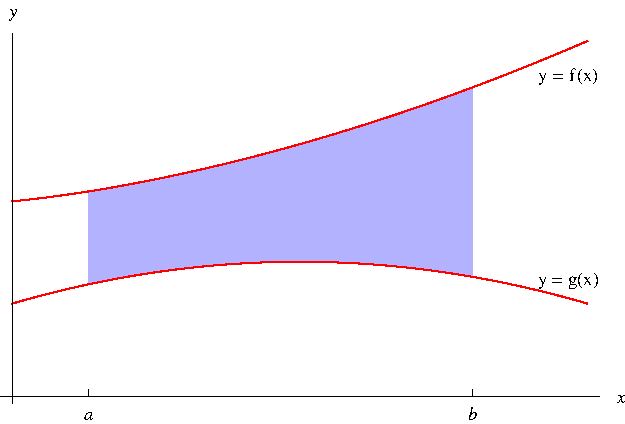
\includegraphics[height=3cm]{area-between-curves/pictures/06-01-doubleint.pdf}
\end{frame}
% end module area-between-curves-intro

% begin module area-between-curves-def
\begin{frame}[t]
\begin{tabular}{|c|c|}
\hline
 \ \ \ \ \ The Area Under a Curve \ \ \ \ \ &
 \ \ \ \ The Area Between Two Curves \ \ \ \ \\
\ \only<1>{%
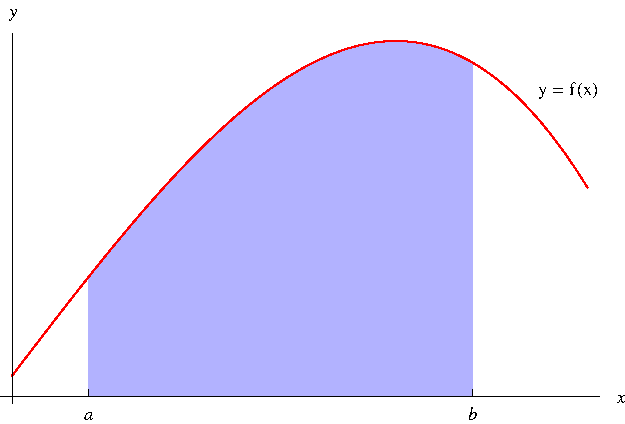
\includegraphics[height=3cm]{area-between-curves/pictures/06-01-singleint.pdf}%
}%
\only<handout:0| 2->{%
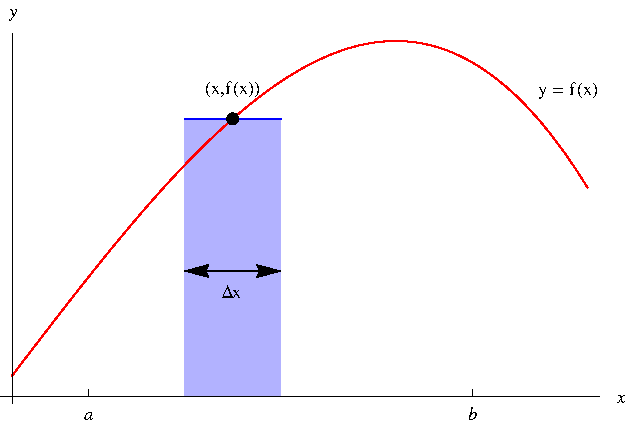
\includegraphics[height=3cm]{area-between-curves/pictures/06-01-1rectangle.pdf}%
}&%
\ \only<-12>{%
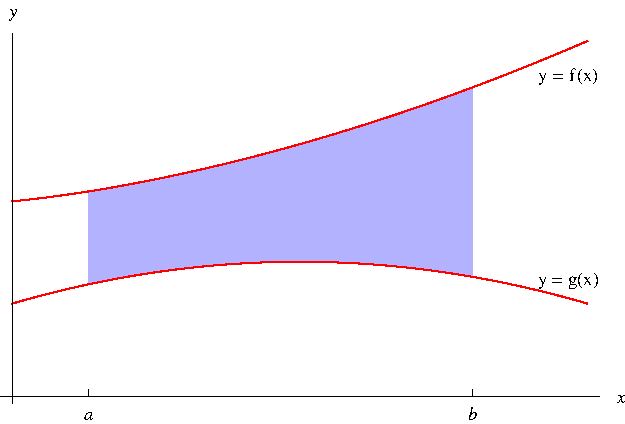
\includegraphics[height=3cm]{area-between-curves/pictures/06-01-doubleint.pdf}%
}%
\only<handout:0| 13->{%
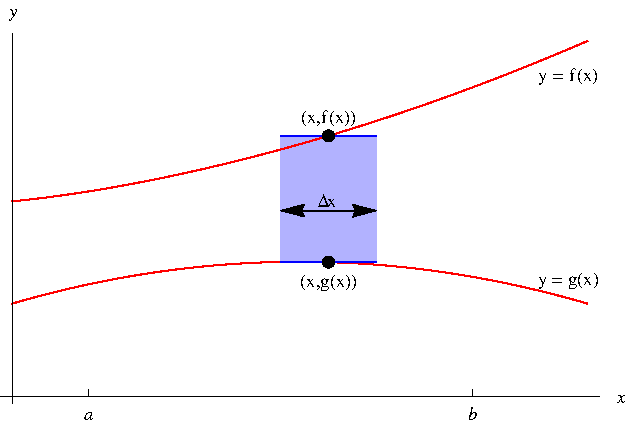
\includegraphics[height=3cm]{area-between-curves/pictures/06-01-1rectanglediff.pdf}%
}\\%
\uncover<2->{
rectangle area $ = $ \only<handout:0| -5>{\alert<handout:0| 5>{height}}\only<6->{\alert<handout:0| 6>{$f(x)$}}$\cdot$\only<handout:0| -3>{\alert<handout:0| 3>{width}}\only<4->{\alert<handout:0| 4>{$\Delta x$}}
} &
\uncover<13->{
rectangle area $ = $ \only<handout:0| -16>{\alert<handout:0| 16>{height}}\only<17->{\alert<handout:0| 17>{$(f(x)-g(x))$}}$\cdot$\only<handout:0| -14>{\alert<handout:0| 14>{width}}\only<15->{\alert<handout:0| 15>{$\Delta x$}}
} \\
\ \only<-7>{%
\uncover<7>{%
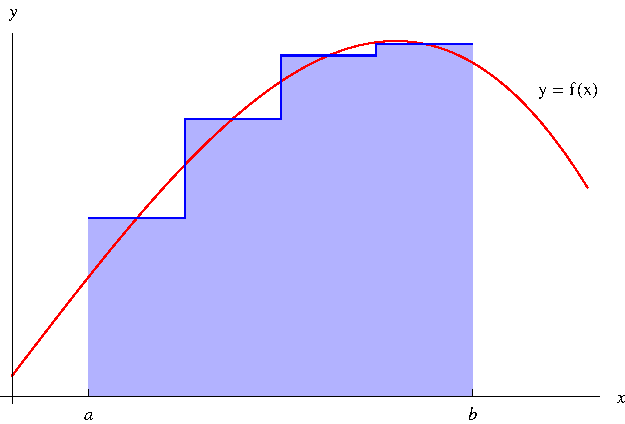
\includegraphics[height=3cm]{area-between-curves/pictures/06-01-4rectangle.pdf}%
}%
}%
\only<handout:0| 8>{%
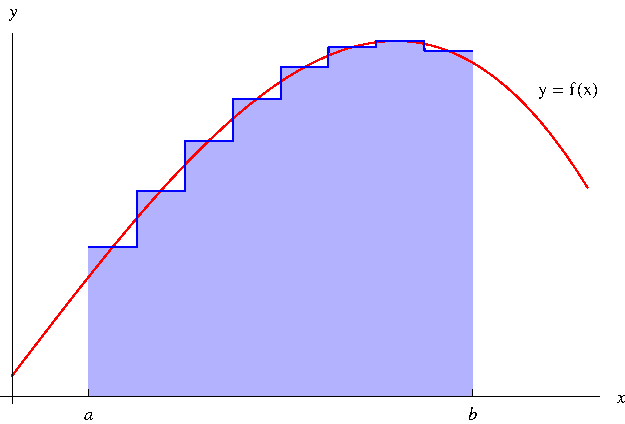
\includegraphics[height=3cm]{area-between-curves/pictures/06-01-8rectangle.pdf}%
}% 
\only<handout:0| 9>{%
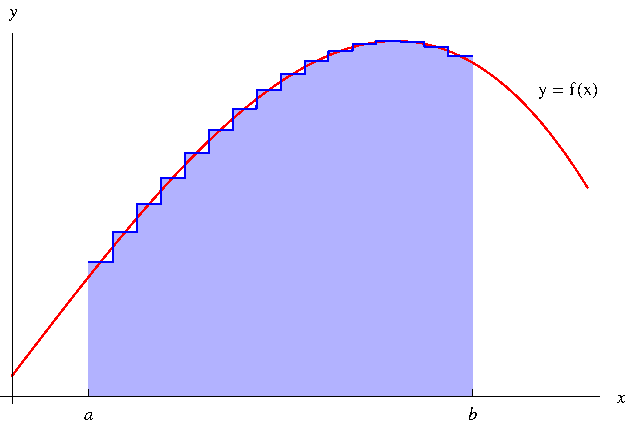
\includegraphics[height=3cm]{area-between-curves/pictures/06-01-16rectangle.pdf}%
}% 
\only<handout:0| 10->{%
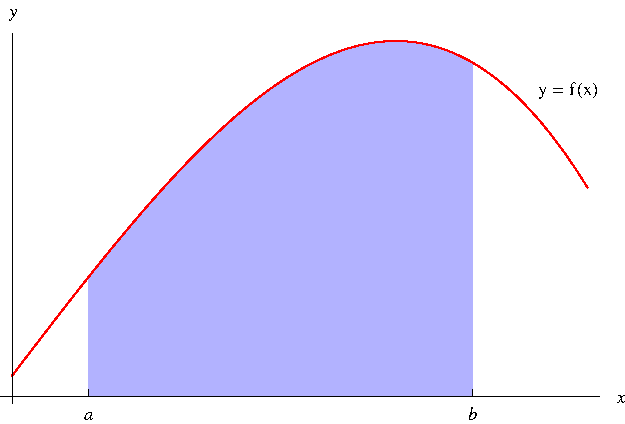
\includegraphics[height=3cm]{area-between-curves/pictures/06-01-singleint.pdf}%
}&%
\ \only<-18>{%
\uncover<18->{%
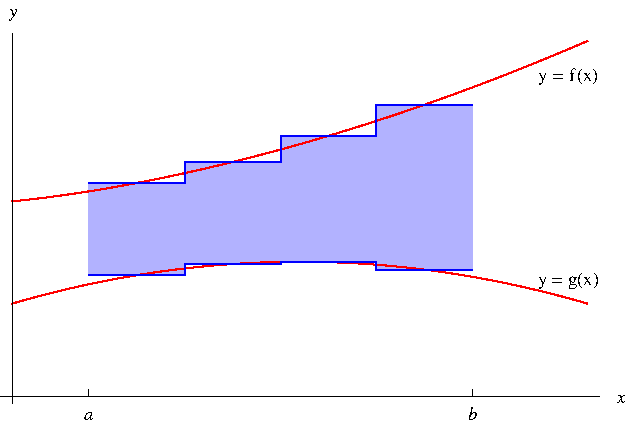
\includegraphics[height=3cm]{area-between-curves/pictures/06-01-4rectanglediff.pdf}%
}%
}%
\only<handout:0| 19>{%
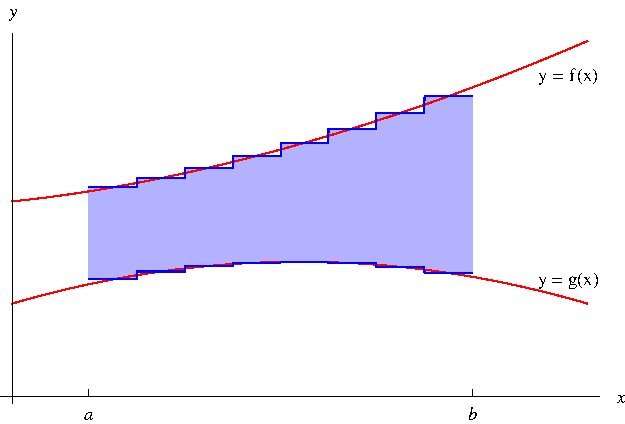
\includegraphics[height=3cm]{area-between-curves/pictures/06-01-8rectanglediff.pdf}%
}%  
\only<handout:0| 20>{%
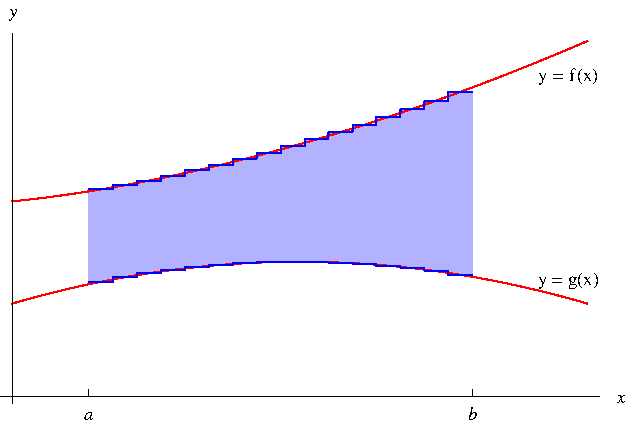
\includegraphics[height=3cm]{area-between-curves/pictures/06-01-16rectanglediff.pdf}%
}%  
\only<handout:0| 21>{%
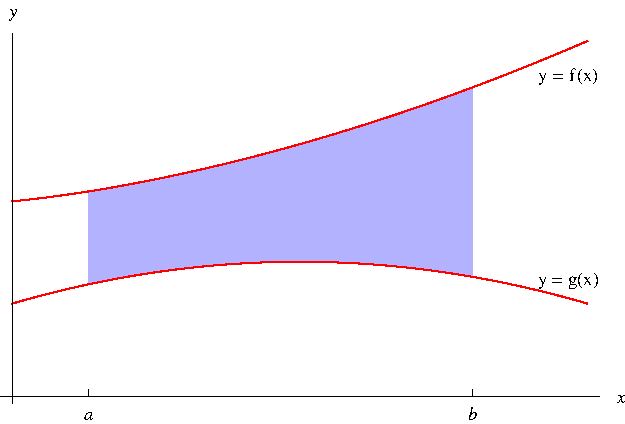
\includegraphics[height=3cm]{area-between-curves/pictures/06-01-doubleint.pdf}%
}\\
\uncover<7->{
\# rectangles $ = \alert<handout:0| 10>{n} \only<handout:0| -9>{=}\only<10->{\alert<handout:0| 10>{\rightarrow}} $ \only<handout:0| -7>{4}\only<handout:0| 8>{\alert<handout:0| 8>{8}}\only<handout:0| 9>{\alert<handout:0| 9>{16}}\only<10->{\alert<handout:0| 10>{$\infty$}}
} & 
\uncover<18->{
\# rectangles $ = n \only<handout:0| -20>{=}\only<21->{\rightarrow} $ \only<handout:0| -18>{4}\only<handout:0| 19>{8}\only<handout:0| 20>{16}\only<21->{$\infty$}
} \\
\only<handout:0| -9,12->{\invisible<1->{$\underset{n\rightarrow \infty}{\lim}$}}%
\uncover<7->{
A  =  \only<handout:0| 10-11>{\alert<handout:0| 10-11>{$\underset{n\rightarrow \infty}{\lim}$}}\only<handout:0| -11>{\alert<handout:0| 11>{$ \sum_{i = 1}^{\only<handout:0| -7>{4}\only<handout:0| 8>{\alert<handout:0| 8>{8}}\only<handout:0| 9>{\alert<handout:0| 9>{16}}\only<handout:0| 10->{\alert<handout:0| 10>{n}}} f(x_i)\Delta x$}}
\only<12->{\alert<handout:0| 12>{$ \int_a^b f(x)\diff x$}}
}% 
\only<-11>{\invisible<1->{$\int_a^b$}}%
& 
\uncover<18->{
A  =  \only<handout:0| -20>{$ \sum_{i = 1}^{\only<handout:0| -18>{4}\only<handout:0| 19>{8}\only<handout:0| 20>{16}} (f(x_i)- g(x_i))\Delta x$}
\only<21->{$ \int_a^b [f(x) - g(x)]\diff x$}
} \\ 
\hline
\end{tabular}
\end{frame}


\begin{frame}
\begin{definition}[The Area Between Two Curves]
The area between two curves $y = f(x)$ and $y = g(x)$ bounded by the endpoints $x = a$ and $x = b$ is
\[ \int_a^b |f(x) - g(x)|\diff x . \]

Note that we use the absolute value, because in general we don't know which curve is above the other.
\end{definition}
\end{frame}
% end module area-between-curves-def

% begin module area-between-curves-ex1
\begin{frame}
\begin{example}%[Example 1, p. 348]
Find the area of the region bounded above by $\alert<handout:0| 3>{y = x^2 + 1}$, bounded below by $\alert<handout:0| 4>{y = x}$, and bounded on its sides by $\alert<handout:0| 6>{x = 0}$ and $\alert<handout:0| 6>{x = 1}$.
\begin{columns}
\column{.4\textwidth}
\psset{xunit=1.5cm, yunit=1.5cm}
\begin{pspicture}(-0.5, -0.5)(1.7,3.7) 
\psframe*[linecolor=white](-0.5,-0.5)(1.7,3.7) 
\tiny 
\psLabels{1.5}{3.5}
\psXTickWithLabel{1}{$1$}
\psYTickWithLabel{1}{$1$}
\psYTickWithLabel{2}{$2$}
\uncover<6->{ %
\pscustom*[linecolor=\psColorAreaUnderGraph]{ %
%Function formula: (x)^{2}+1 
\psplot[linecolor=\psColorGraph, plotpoints=1000]{0}{1}{1 x 2 exp add }
%Function formula: x 
\psplot[linecolor=\psColorGraph, plotpoints=1000]{1}{0}{x}
} %
\rput[r](-0.05,0.5){$x=0$}
\rput[l](1.05,1.5){$x=1$}
} %
\only<3->{
\rput(1,3){$y=x^{2}+1$} 
%Function formula: (x)^{2}+1 
\psplot[linecolor=\psColorGraph, plotpoints=1000]{-0.5}{1.5}{1 x 2 exp add }
}
\only<4->{
\rput[rt](1.5,1){$y=x$} 
%Function formula: x 
\psplot[linecolor=\psColorGraph, plotpoints=1000]{-0.47}{1.5}{x}
}
\psaxes[ticks=none, labels=none]{<->}(0,0)(-0.5,-0.5)(1.5,3.5)
\end{pspicture} 
%\ \only<handout:0| -2>{%
%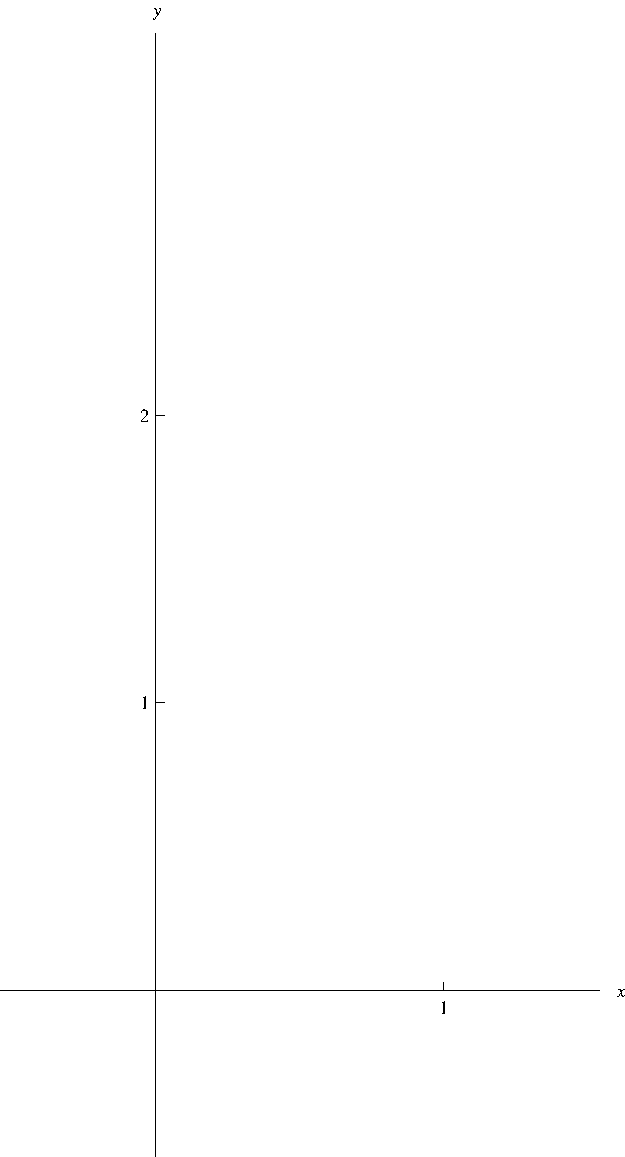
\includegraphics[height=6.5cm]{area-between-curves/pictures/06-01-ex1a.pdf}%
%}%  
%\only<handout:0| 3>{%
%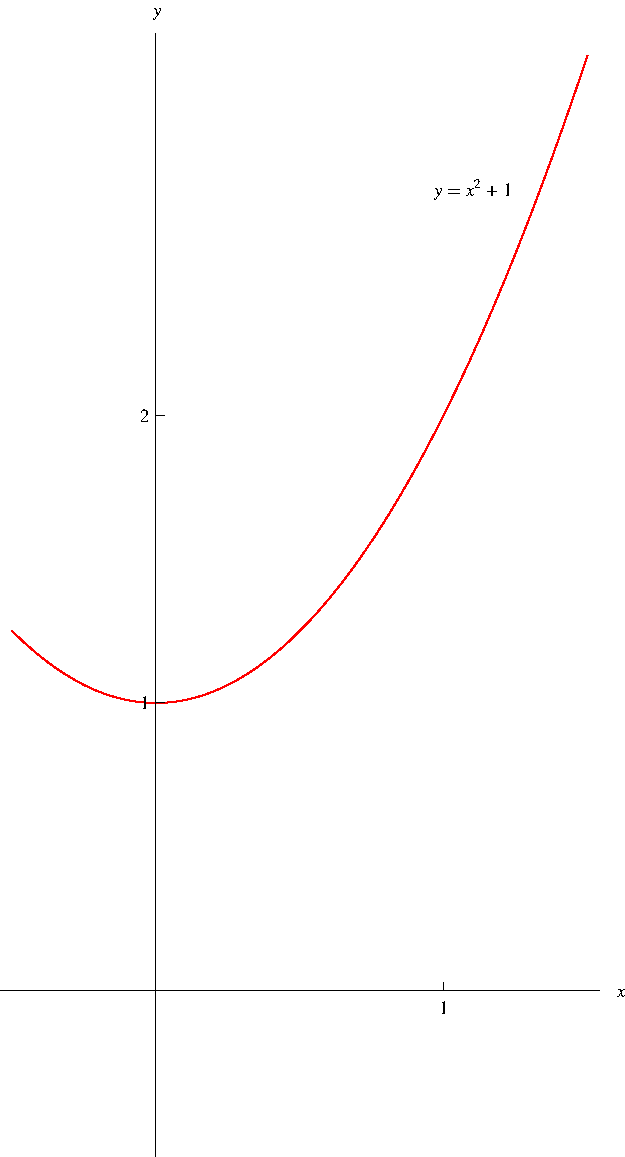
\includegraphics[height=6.5cm]{area-between-curves/pictures/06-01-ex1b.pdf}%
%}%  
%\only<handout:0| 4-5>{%
%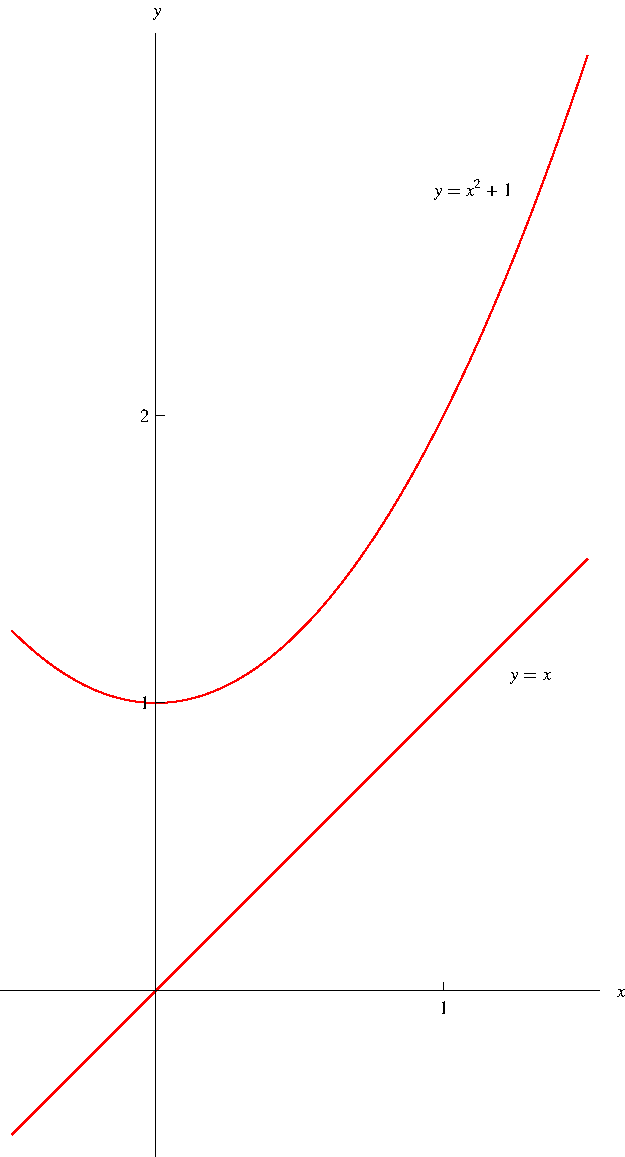
\includegraphics[height=6.5cm]{area-between-curves/pictures/06-01-ex1c.pdf}%
%}%  
%\only<6->{%
%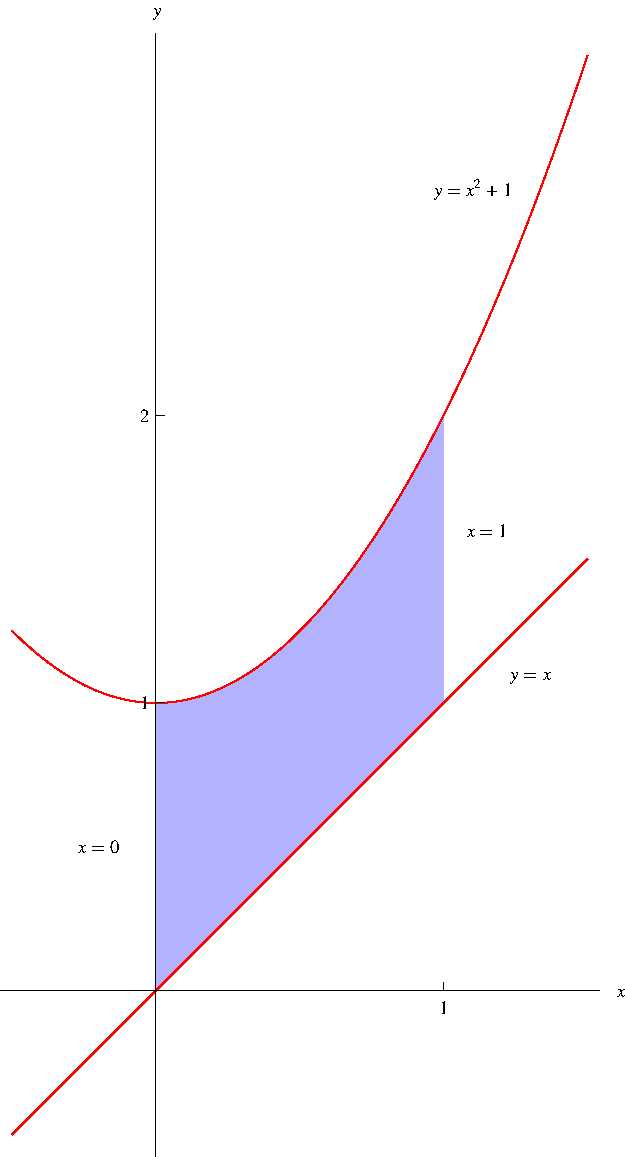
\includegraphics[height=6.5cm]{area-between-curves/pictures/06-01-ex1d.pdf}%
%}%  

\column{.6\textwidth}
\begin{enumerate}
\item<2->  Graph the functions.
\item<5->  Identify the region.
\item<7->  Integrate.
\end{enumerate}
\abovedisplayskip=0pt
\belowdisplayskip=0pt
\abovedisplayshortskip=0pt
\belowdisplayshortskip=0pt
\begin{align*}
\uncover<8->{A} & \uncover<8->{=}  \uncover<8->{\int_0^1 |(x^2 + 1) - x|\diff x} \\
 &  \uncover<8->{=}  \uncover<8->{\int_0^1 ( x^2 - x + 1 ) \diff x} \\
 & \uncover<9->{=}  \uncover<9->{\left[  \frac{x^3}{3} - \frac{x^2}{2} + x \right]_0^1} \\
 & \uncover<10->{=}  \uncover<10->{ \frac{1}{3} - \frac{1}{2} + 1 } \uncover<11->{  = \frac{5}{6}. } 
\end{align*}
\end{columns}
\end{example}
\end{frame}
% end module area-between-curves-ex1

% begin module area-between-curves-ex2
\begin{frame}
\begin{example} %[Example 2, p. 433]
\begin{columns}
\column{.35\textwidth}
\psset{xunit=1.5cm, yunit=1.5cm}
\begin{pspicture}(-0.5, -0.5)(1.5,2.7) 
\psframe*[linecolor=white](-0.5,-0.5)(1.7,2.7) 
\tiny 
\psaxes[ticks=none, labels=none]{<->}(0,0)(-0.5,-0.5)(1.5,2.5)
\psLabels{1.5}{2.5}
\psXTickWithLabel{1}{$1$}
\psYTickWithLabel{1}{$1$}
\psYTickWithLabel{2}{$2$}

\uncover<6->{
\psFullDot{1}{1}
\rput[bl](1.1,1){$(1,1)$}
\psFullDot{0}{0}
\rput[tl](0.05,-0.05){$(0,0)$}
}

\uncover<11->{ %
\pscustom*[linecolor=\psColorAreaUnderGraph]{ %
%Function formula: 2 (x)- ((x)^{2}) 
\psplot[linecolor=\psColorGraph, plotpoints=1000]{0}{1}{x 2 exp -1 mul x 2 mul add }
%Function formula: (x)^{2} 
\psplot[linecolor=\psColorGraph, plotpoints=1000]{1}{0}{x 2 exp }
} %
} %
\uncover<9->{ %
%Function formula: 2 (x)- ((x)^{2}) 
\rput[l](-0.4,0.7){$y=2 x- x^{2}$} 
\psplot[linecolor=\psColorGraph, plotpoints=1000]{-0.2}{1.5}{x 2 exp -1 mul x 2 mul add }
} %
\uncover<8->{ %
%Function formula: (x)^{2} 
\rput[r](1.3,2){$y=x^{2}$} 
\psplot[linecolor=\psColorGraph, plotpoints=1000]{-0.2}{1.5}{x 2 exp }
} %
\end{pspicture} 
%\ \only<handout:0| -5>{%
%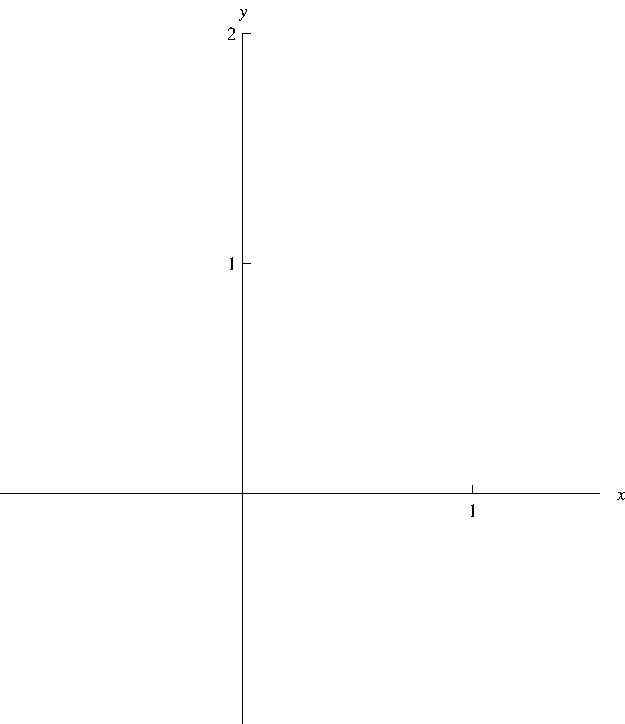
\includegraphics[height=4cm]{area-between-curves/pictures/06-01-ex2a.pdf}%
%}%  
%\only<handout:0| 6-7>{%
%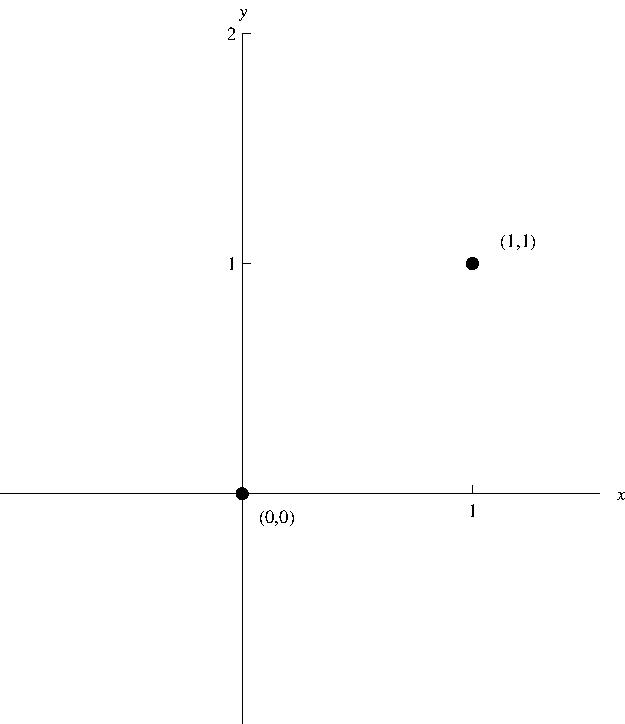
\includegraphics[height=4cm]{area-between-curves/pictures/06-01-ex2b.pdf}%
%}%  
%\only<handout:0| 8>{%
%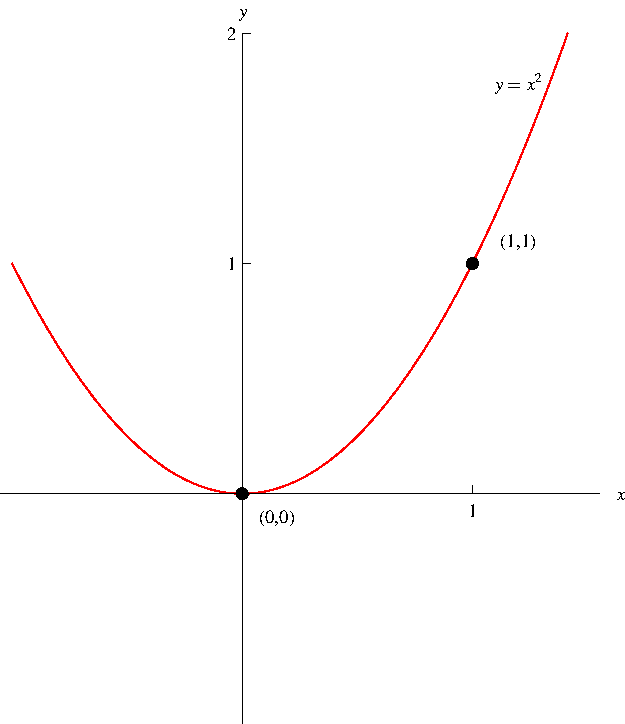
\includegraphics[height=4cm]{area-between-curves/pictures/06-01-ex2c.pdf}%
%}%  
%\only<handout:0| 9-10>{%
%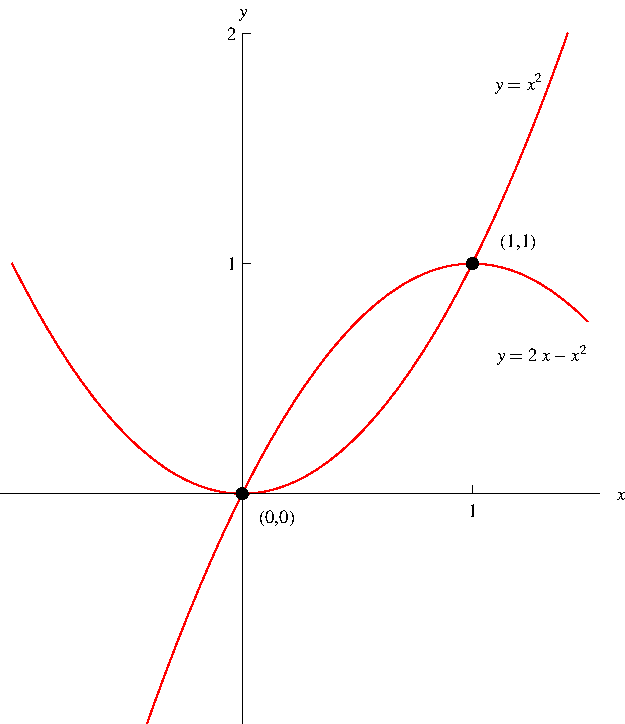
\includegraphics[height=4cm]{area-between-curves/pictures/06-01-ex2d.pdf}%
%}%  
%\only<11->{%
%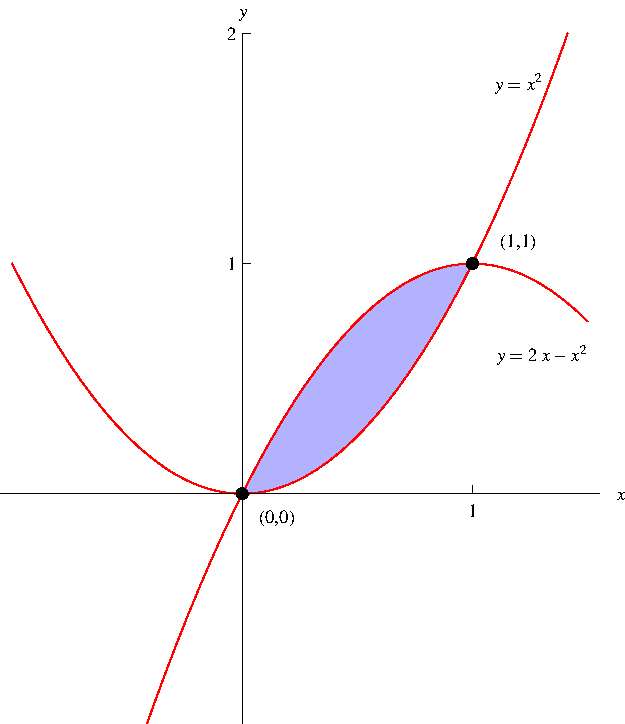
\includegraphics[height=4cm]{area-between-curves/pictures/06-01-ex2e.pdf}%
%}%  
\begin{enumerate}
\item<2->  Find the point of intersection.
\item<7->  Graph the functions.
\item<10->  Identify the region.
\item<12->  Integrate.
\end{enumerate}

\column{.65\textwidth}
Find the area of the region enclosed by the parabolas $\alert<handout:0| 8>{y =} \alert<handout:0| 3,8>{x^2}$ and $\alert<handout:0| 9>{y =} \alert<handout:0| 3,9>{2x - x^2}$.
\abovedisplayskip=0pt
\belowdisplayskip=0pt
\abovedisplayshortskip=0pt
\belowdisplayshortskip=0pt
\begin{align*}
\uncover<3->{\alert<handout:0| 3>{x^2}} & \uncover<3->{\alert<handout:0| 3>{=}}  \uncover<3->{\alert<handout:0| 3>{2x - x^2}} \\
\uncover<4->{0} & \uncover<4->{=}  \uncover<4->{2x - 2x^2} \uncover<5->{ = 2x(1 - x)} \\
\uncover<6->{x} & \uncover<6->{=}  \uncover<6->{0 \text{ or } 1.}
\end{align*}
\begin{align*}
\uncover<13->{A} & \uncover<13->{=}  \uncover<13->{\int_0^1 (2x - 2x^2) \diff x} \uncover<14->{ = 2\int_0^1 (x - x^2) \diff x} \\
 & \uncover<15->{=}  \uncover<15->{2\left[ \frac{x^2}{2} - \frac{x^3}{3}\right]_0^1} \uncover<16->{ = 2\left( \frac{1}{2} - \frac{1}{3}\right)} \uncover<17->{ = \frac{1}{3}.}
\end{align*}
\end{columns}
\end{example}
\end{frame}
% end module area-between-curves-ex2

% begin module area-between-curves-ex5
\begin{frame}
\begin{example}%[Example 5, p. 350]
\begin{columns}
\column{.35\textwidth}
\ \ \only<handout:0| -2>{%
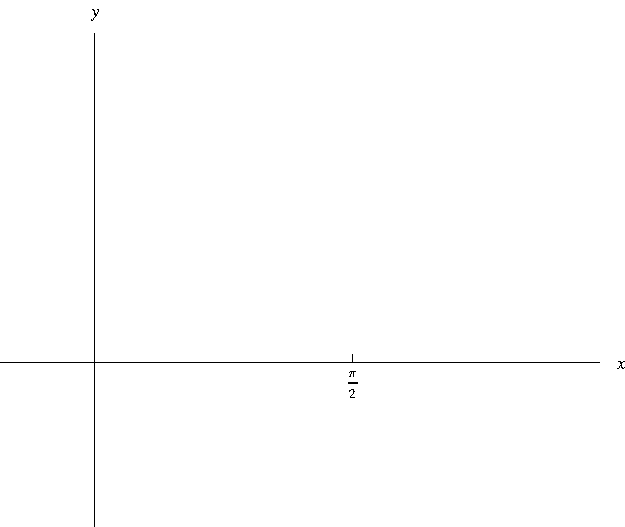
\includegraphics[height=3cm]{area-between-curves/pictures/06-01-ex5a.pdf}%
}%  
\only<handout:0| 3-4>{%
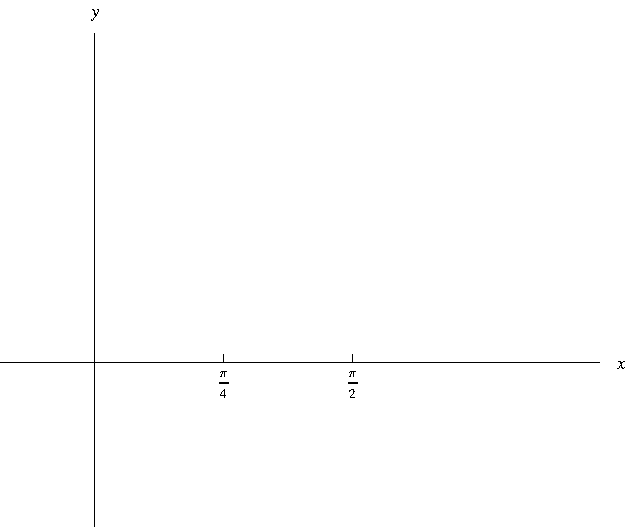
\includegraphics[height=3cm]{area-between-curves/pictures/06-01-ex5b.pdf}%
}%  
\only<handout:0| 5>{%
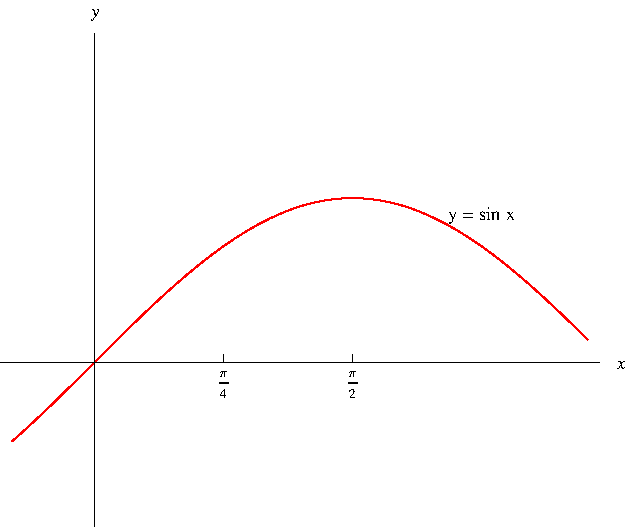
\includegraphics[height=3cm]{area-between-curves/pictures/06-01-ex5c.pdf}%
}%  
\only<handout:0| 6-7>{%
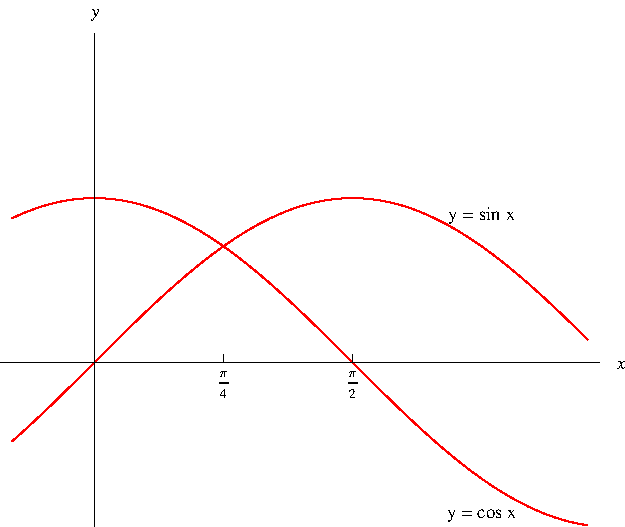
\includegraphics[height=3cm]{area-between-curves/pictures/06-01-ex5d.pdf}%
}%  
\only<8->{%
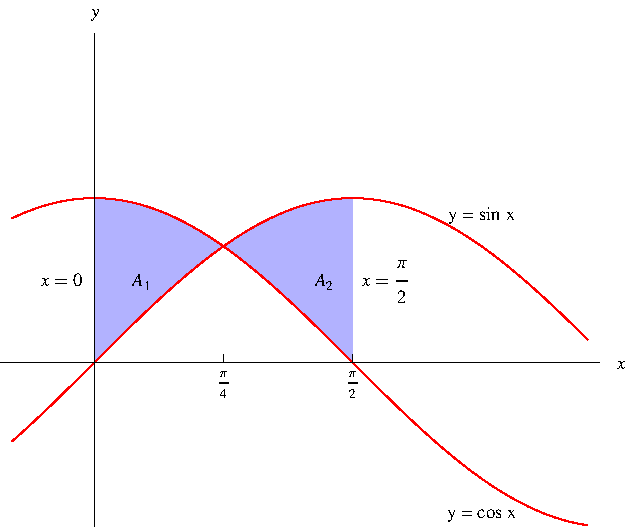
\includegraphics[height=3cm]{area-between-curves/pictures/06-01-ex5e.pdf}%
}%  
\begin{enumerate}
\item<2->  Find the point of intersection.
\item<4->  Graph the functions.
\item<7->  Identify the region.
\item<9->  Integrate.
\end{enumerate}

\column{.7\textwidth}
Find the area of the region enclosed by the curves $\alert<handout:0| 5>{y =} \alert<handout:0| 5>{\sin x}$, $\alert<handout:0| 6>{y =} \alert<handout:0| 6>{\cos x}$, $\alert<handout:0| 8>{x = 0}$ and $\alert<handout:0| 8>{x = \pi/2}$.

\uncover<3->{The only point of intersection in the interval $[0,\pi /2]$ is $(\pi /4, 1/\sqrt{2} )$.}
\abovedisplayskip=0pt
\belowdisplayskip=0pt
\abovedisplayshortskip=0pt
\belowdisplayshortskip=0pt
\begin{align*}
\uncover<8->{A} & \uncover<8->{ = A_1 + A_2} \\%
 & \uncover<9->{=}  \uncover<9->{\int_0^{\pi /4} (\cos x - \sin x )\diff x} \\
&  \qquad \uncover<9->{+ \int_{\pi /4}^{\pi /2} (\sin x - \cos x)\diff x} \\
 & \uncover<10->{=}  \uncover<10->{\left[ \sin x + \cos x \right]_0^{\pi / 4} + \left[ -\cos x - \sin x\right]_{\pi /4}^{\pi /2}}  \\
% & \uncover<11->{=}  \uncover<11->{\left[ \left( \frac{\sqrt{2}}{2} + \frac{\sqrt{2}}{2}\right) - \left( 0 + 1\right)\right] + \left[ \left( -0 - 1\right) - \left( -\frac{\sqrt{2}}{2} - \frac{\sqrt{2}}{2}\right) \right]}\\
% & \uncover<11->{=}  \uncover<11->{\left(  \frac{1}{\sqrt{2}} + \frac{1}{\sqrt{2}} - 0 - 1\right) + \left( -0 - 1 + \frac{1}{\sqrt{2}} + \frac{1}{\sqrt{2}}\right)}  \\
 & \uncover<11->{=}  \uncover<11->{2\sqrt{2} - 2.}%
\end{align*}
\end{columns}
\end{example}
\end{frame}
% end module area-between-curves-ex5

\section{(6.2) Volumes}
% begin module volumes-intro
\begin{frame}
\frametitle{Volumes}
\begin{center}
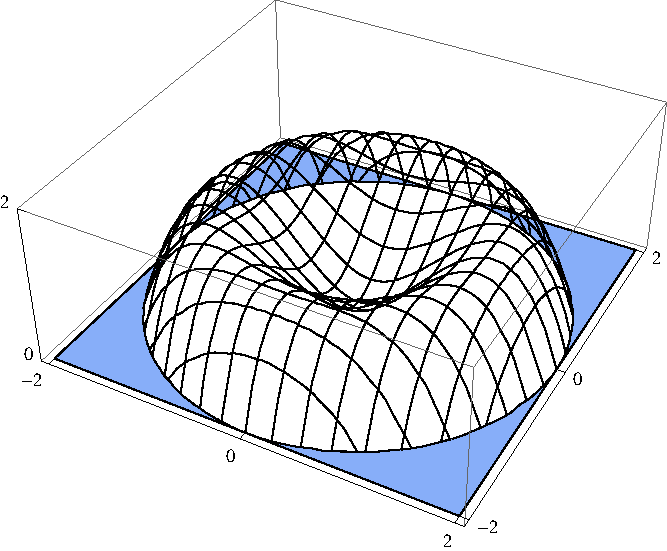
\includegraphics[height=6.5cm]{volumes/pictures/06-03-setup3d.pdf} %

We can use integration to find the volumes of certain solids.%
\end{center}
\end{frame}

\begin{frame}
\begin{columns}[c]
\column{.35\textwidth}
\only<handout:1| -1>{%
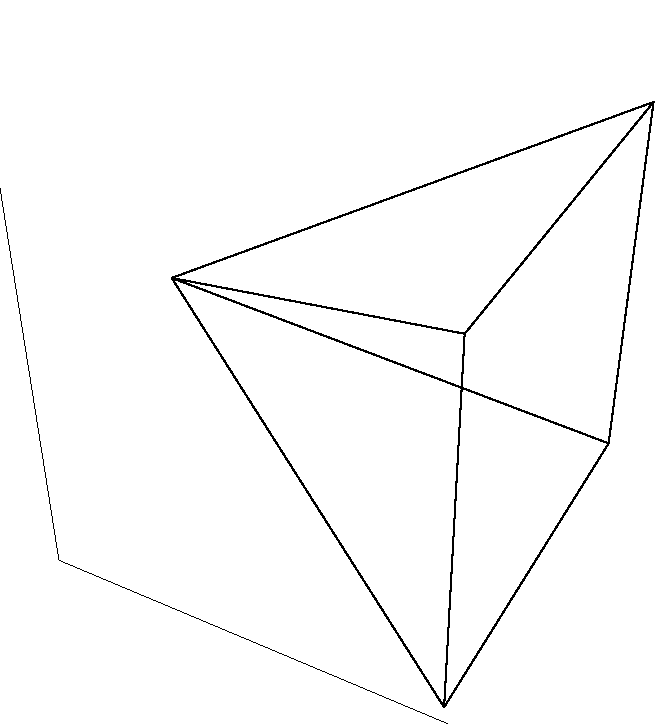
\includegraphics[height=4cm]{volumes/pictures/06-02-pyramida.pdf} %
}%
\only<handout:0| 2>{%
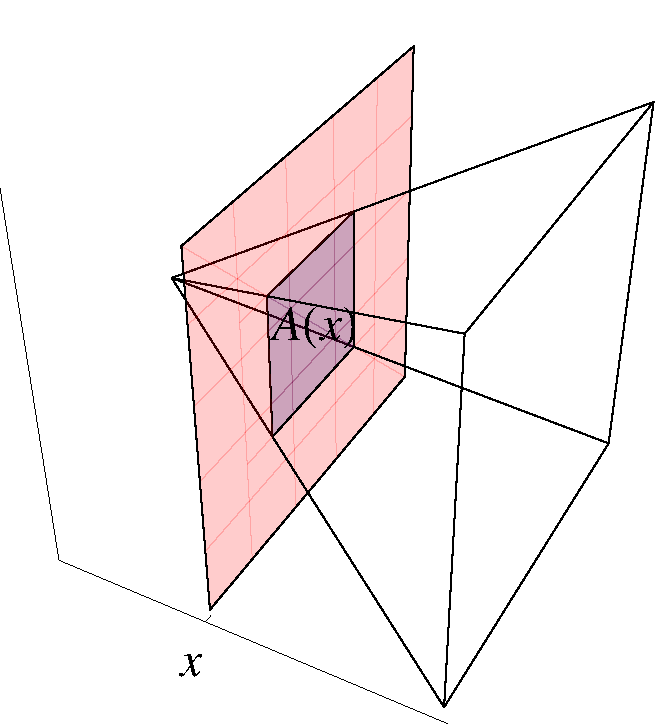
\includegraphics[height=4cm]{volumes/pictures/06-02-pyramidb.pdf}%
}%
\only<handout:0| 3>{%
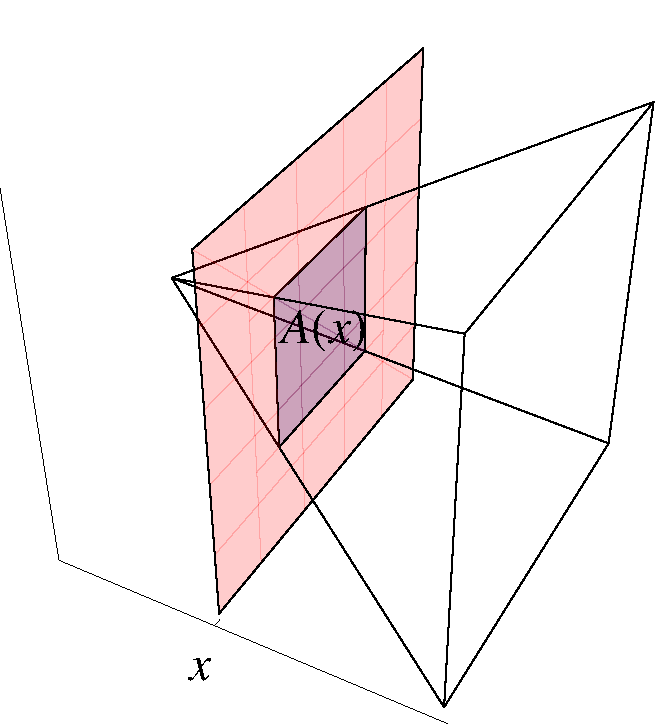
\includegraphics[height=4cm]{volumes/pictures/06-02-pyramidc.pdf}%
}%
\only<handout:0| 4>{%
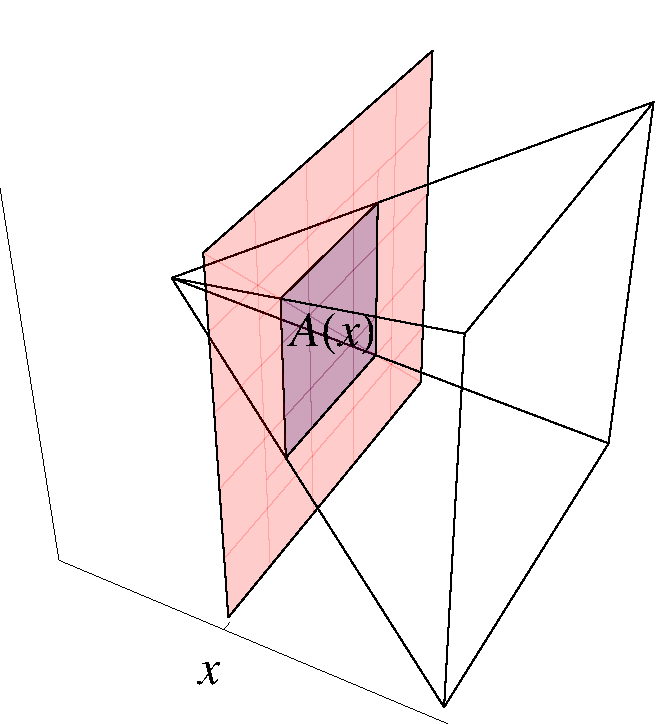
\includegraphics[height=4cm]{volumes/pictures/06-02-pyramidd.pdf}%
}%
\only<handout:2| 5>{%
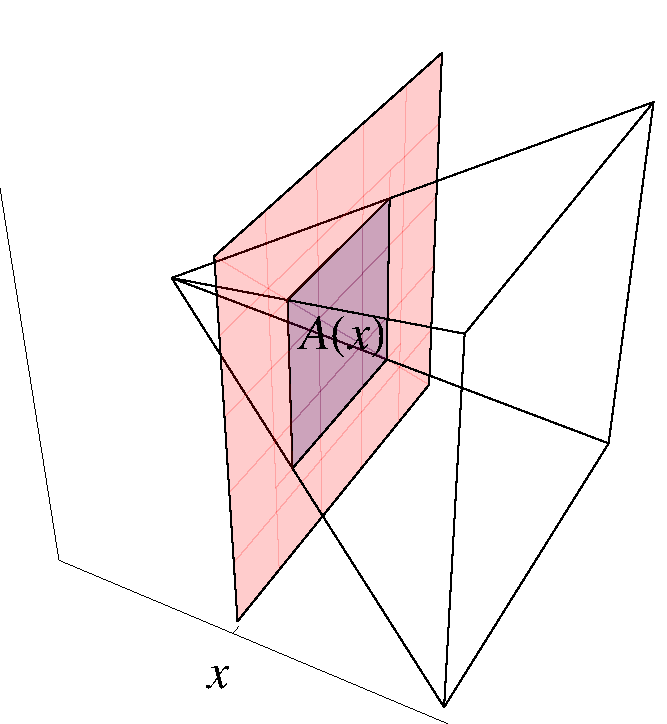
\includegraphics[height=4cm]{volumes/pictures/06-02-pyramide.pdf}%
}%
\only<handout:0| 6-7>{%
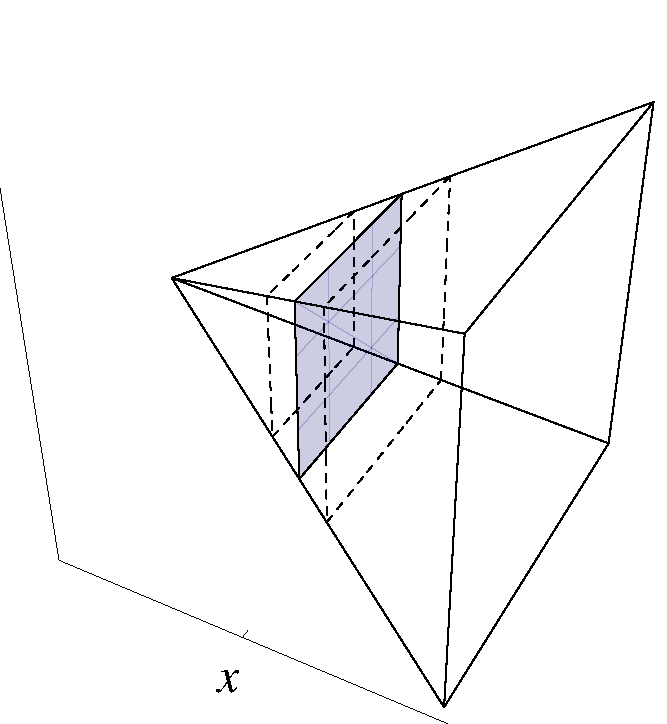
\includegraphics[height=4cm]{volumes/pictures/06-02-pyramidf.pdf}%
}%
\only<handout:3| 8->{%
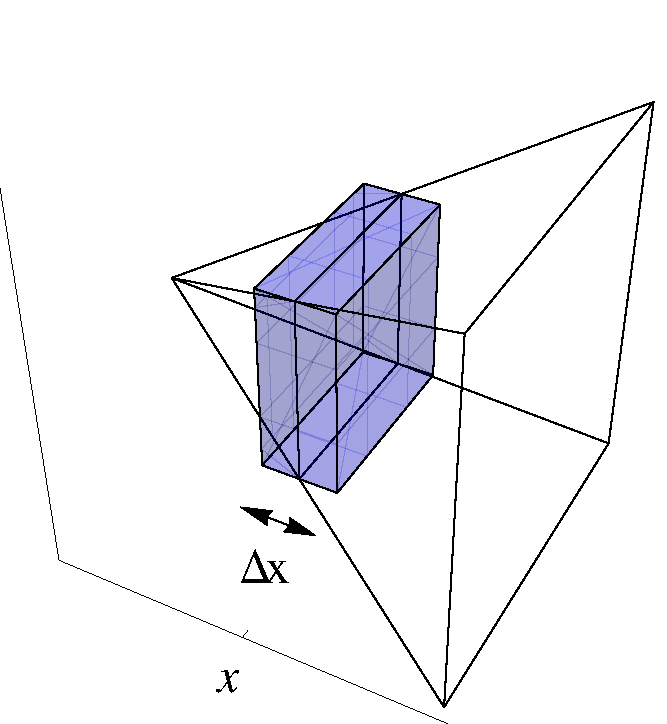
\includegraphics[height=4cm]{volumes/pictures/06-02-pyramidg.pdf}%
}%

\uncover<handout:3| 9->{Approx. volume of slab:}
\abovedisplayskip=1pt
\belowdisplayskip=1pt
\[
\uncover<handout:3| 9->{A(x^*)\Delta x}%
\]
\uncover<handout:3| 10->{Approx. volume of $S$:}
\abovedisplayskip=1pt
\belowdisplayskip=1pt
\[
\uncover<handout:3| 10->{V \approx \sum_{i=1}^n A(x_i^*)\Delta x}%
\]
\uncover<handout:3| 11->{Exact volume of $S$:}
\abovedisplayskip=1pt
\belowdisplayskip=1pt
\[
\uncover<handout:3| 11->{V = \lim_{n\to\infty}\sum_{i=1}^n A(x_i^*)\Delta x}%
\]
\column{.65\textwidth}
\begin{itemize}
\item  How do we find the volume of a solid $S$?
\item<handout:2-| 2->  Let $P_x$ be the plane perpendicular to the $x$-axis and passing through the point $x$.
\item<handout:2-| 2->  The intersection of $P_x$ with $S$ is called a cross-section.
\item<handout:2-| 2->  Let $A(x)$ be the area of this cross-section.
\item<handout:3| 6->  Consider the part of $S$ between two planes $P_{x_1}$ and $P_{x_2}$.
\item<handout:3| 7->  Approximate this part of $S$:
\item<handout:3| 7->  Pick a sample point $x^*$ between $x_1$ and $x_2$.  Use a solid that has the same constant cross-sectional area $A(x^*)$ between $x_1$ and $x_2$.
\item<handout:3| 8->  Let $\Delta x$ be the distance from $x_1$ to $x_2$.
\end{itemize}
\end{columns}
\end{frame}
% end module volumes-intro

% begin module volumes-def
\begin{frame}
\begin{definition}[Volume]
Let $S$ be a solid that lies between $x = a$ and $x = b$.  If the cross-sectional area of $S$ in the plane $P_x$ is a continuous function $A(x)$, then the volume of $S$ is
\[
V = \lim_{n\to\infty} \sum_{i=1}^n A(x_i^*)\Delta x = \int_a^b A(x)\diff x%
\]
\end{definition}
\end{frame}
% end module volumes-def

% begin module volumes-ex2
\begin{frame}
\begin{example}[Example 2, p. 356]
Find the volume of the solid obtained by rotating about the $x$-axis the region under the curve $y = \sqrt{x}$ from $0$ to $1$.
\begin{itemize}
\item<8->  The cross-sections of this solid are all circles.
\item<9->  The circular cross-section through the point $(x, 0)$ has radius $\sqrt{x}$.
\item<10->  The area of the cross-section is \alert<handout:0| 10-11>{$A(x) = $ \uncover<11->{$\pi (\sqrt{x})^2$}} \uncover<12->{$ = \pi x$.}
\item<13->  The volume of a single approximating section is $A(x) \Delta x = \pi x \ \Delta x$.
\item<14->  The solid lies between $0$ and $1$, so its volume is
\end{itemize}
\begin{columns}[c]
\column{.4\textwidth}
\begin{center}
\only<handout:0| 1>{%
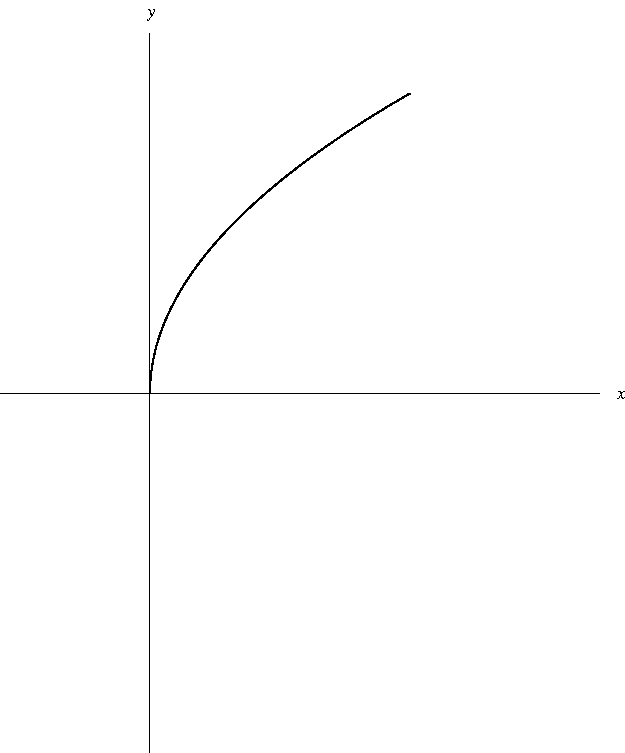
\includegraphics[height=3.5cm]{volumes/pictures/06-02-ex2a.pdf} %
}%
\only<handout:0| 2>{%
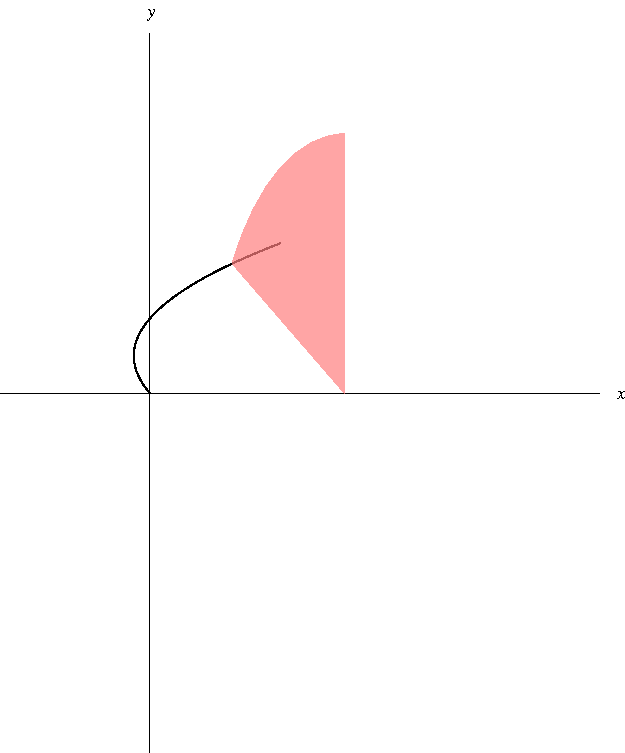
\includegraphics[height=3.5cm]{volumes/pictures/06-02-ex2b.pdf} %
}%
\only<handout:0| 3>{%
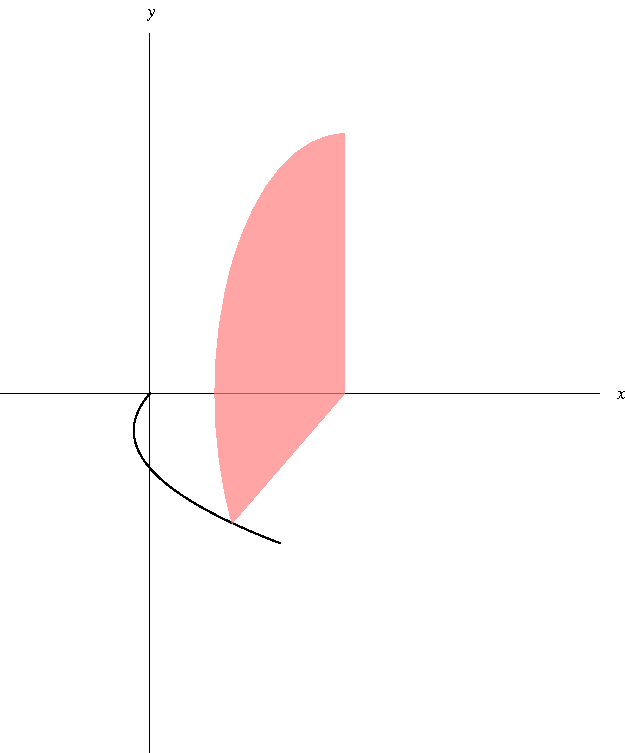
\includegraphics[height=3.5cm]{volumes/pictures/06-02-ex2c.pdf} %
}%
\only<handout:0| 4>{%
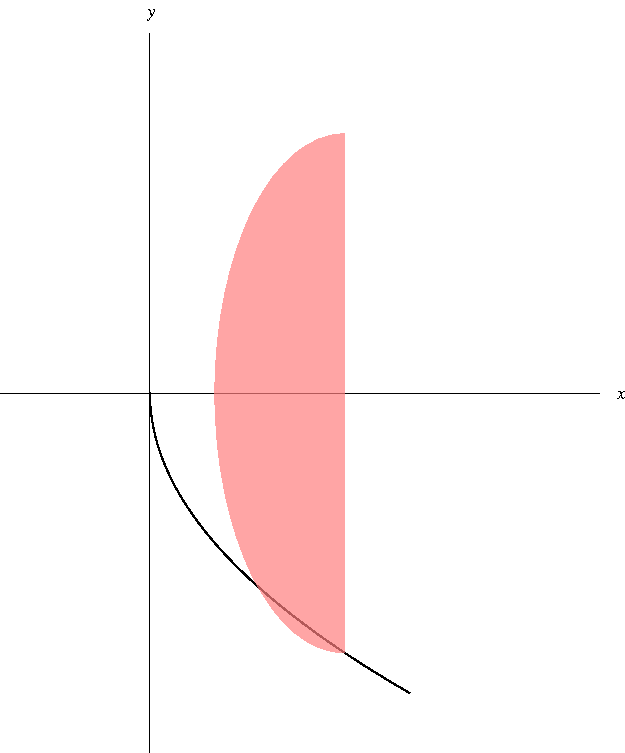
\includegraphics[height=3.5cm]{volumes/pictures/06-02-ex2d.pdf} %
}%
\only<handout:0| 5>{%
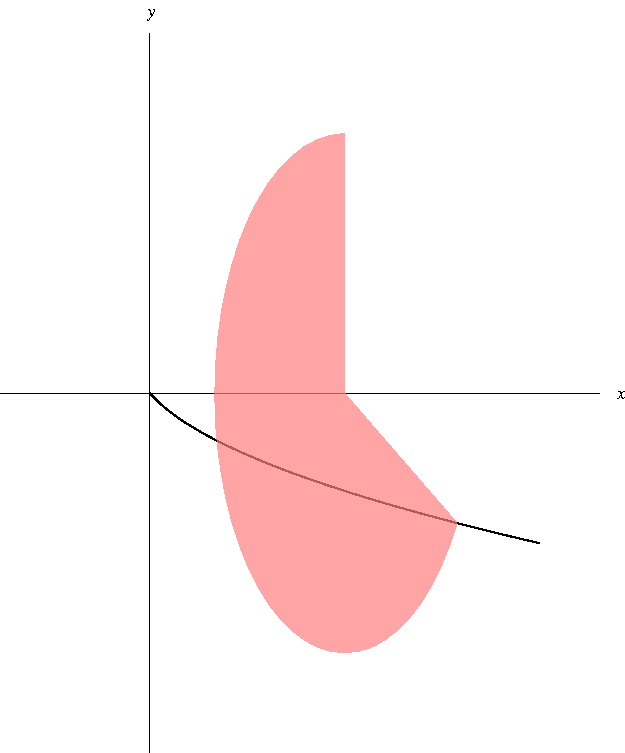
\includegraphics[height=3.5cm]{volumes/pictures/06-02-ex2e.pdf} %
}%
\only<handout:0| 6>{%
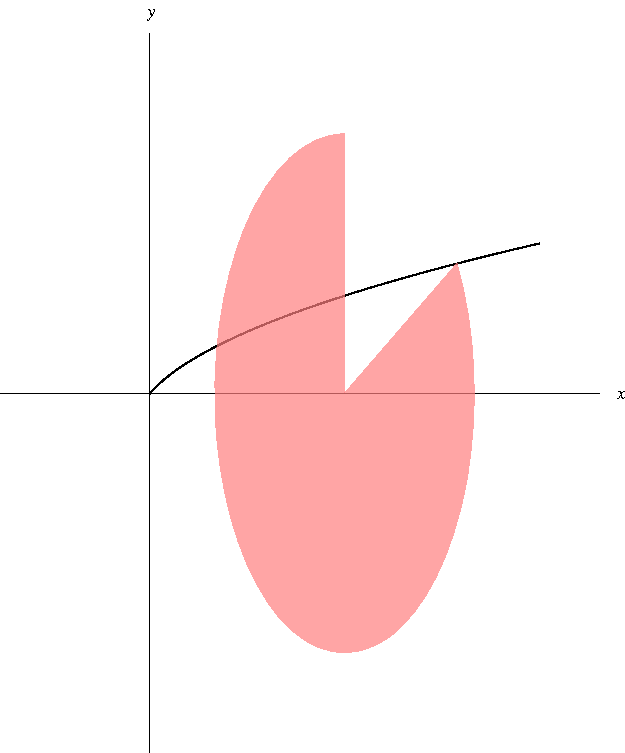
\includegraphics[height=3.5cm]{volumes/pictures/06-02-ex2f.pdf} %
}%
\only<7->{%
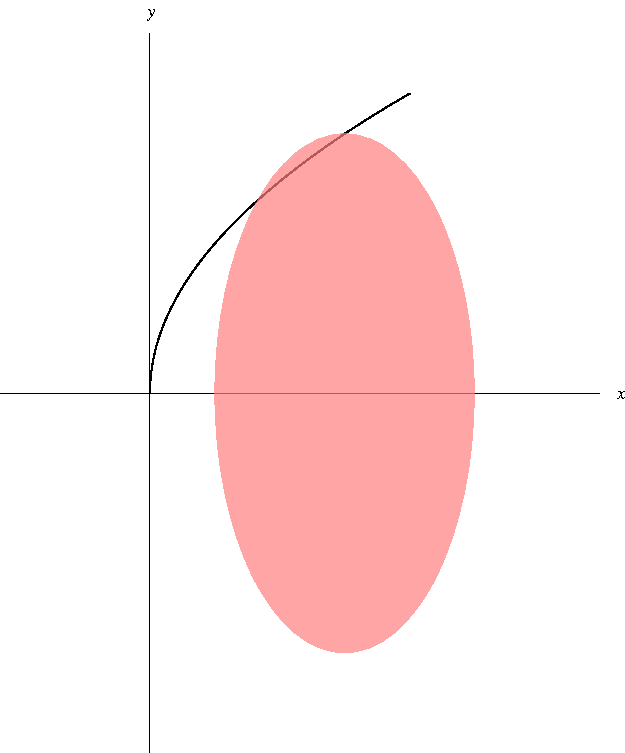
\includegraphics[height=3.5cm]{volumes/pictures/06-02-ex2g.pdf} %
}%
\end{center}
\column{.6\textwidth}
\abovedisplayskip=0pt
\belowdisplayskip=0pt
\begin{eqnarray*}
\uncover<14->{%
V%
}%
& \uncover<14->{ = } &%
\uncover<14->{%
\int_0^1 A(x) \ \diff x%
}%
 \uncover<15->{ = } %
\uncover<15->{%
\int_0^1 \pi x \ \diff x%
}\\%
& \uncover<16->{ = } &%
\uncover<16->{%
\left[ \pi \frac{x^2}{2}\right]_0^1%
}%
 \uncover<17->{ = } %
\uncover<17->{%
\frac{\pi}{2}%
}%
\end{eqnarray*}
\end{columns}
\end{example}
\end{frame}
% end module volumes-ex2

% begin module volumes-washer
\begin{frame}
\begin{example}[Typical Cross-Section is a Washer]
\begin{columns}[c]
\column{.35\textwidth}
\psset{xunit=1cm, yunit=1cm}
\begin{pspicture}(-1,-1)(1,1)
\tiny%
\renewcommand{\fcScreenStyle}{x}%
\renewcommand{\fcScreen}{[0 0 -1] 0}%
\renewcommand{\fcIterationsU}{4}%
\fcBoundingBox{-1.8}{-1.8}{1.8}{1.8}
\only<3->{\renewcommand{\fcScreen}{[-0.05 -0.05 -1] 0}}%
\only<4->{\renewcommand{\fcScreen}{[-0.1 -0.1 -1] 0}}%
\only<5->{\renewcommand{\fcScreen}{[-0.15 -0.15 -1] 0}}%
\only<6->{\renewcommand{\fcScreen}{[-0.2 -0.2 -1] 0}}%
\only<7->{\renewcommand{\fcScreen}{[-0.25 -0.25 -1] 0}}%
\fcStartIIIdScene%
\only<3->{\fcPutIIId{[-0.1 -0.1 1.6]}{$z$}}%
\fcAxesIIIdInScene[arrows=->, xLabel={$x$}, yLabel={$y$},zLabel={} ]{1.5}{1.5}{1.5}%
\fcFinishIIIdScene
\end{pspicture}

\only<handout:0| 1>{%
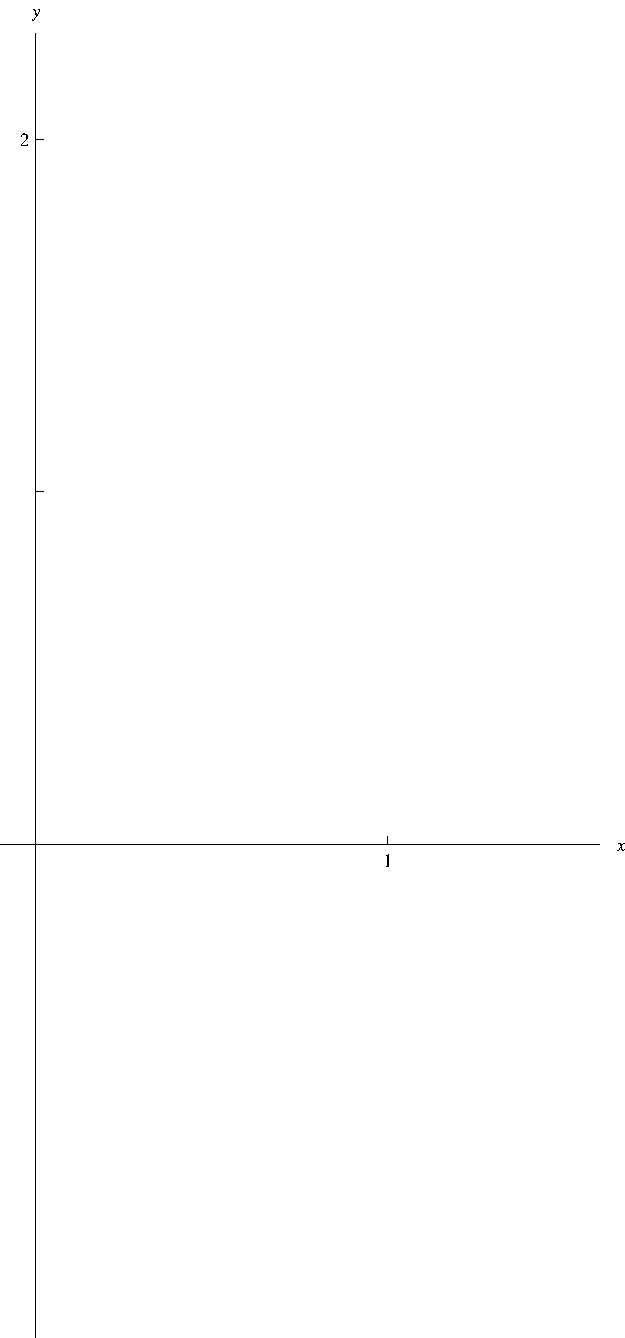
\includegraphics[height=3.3cm]{volumes/pictures/06-02-washera.pdf} %
}%
\only<handout:0| 2>{%
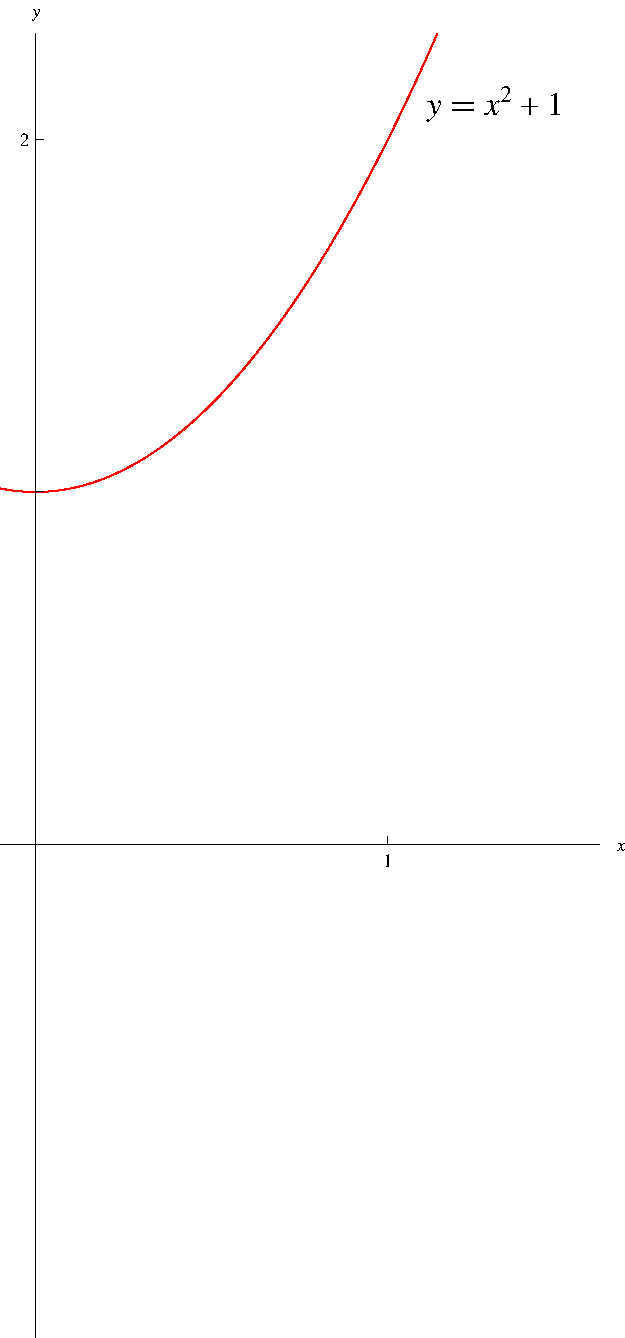
\includegraphics[height=3.3cm]{volumes/pictures/06-02-washerb.pdf} %
}%
\only<handout:0| 3>{%
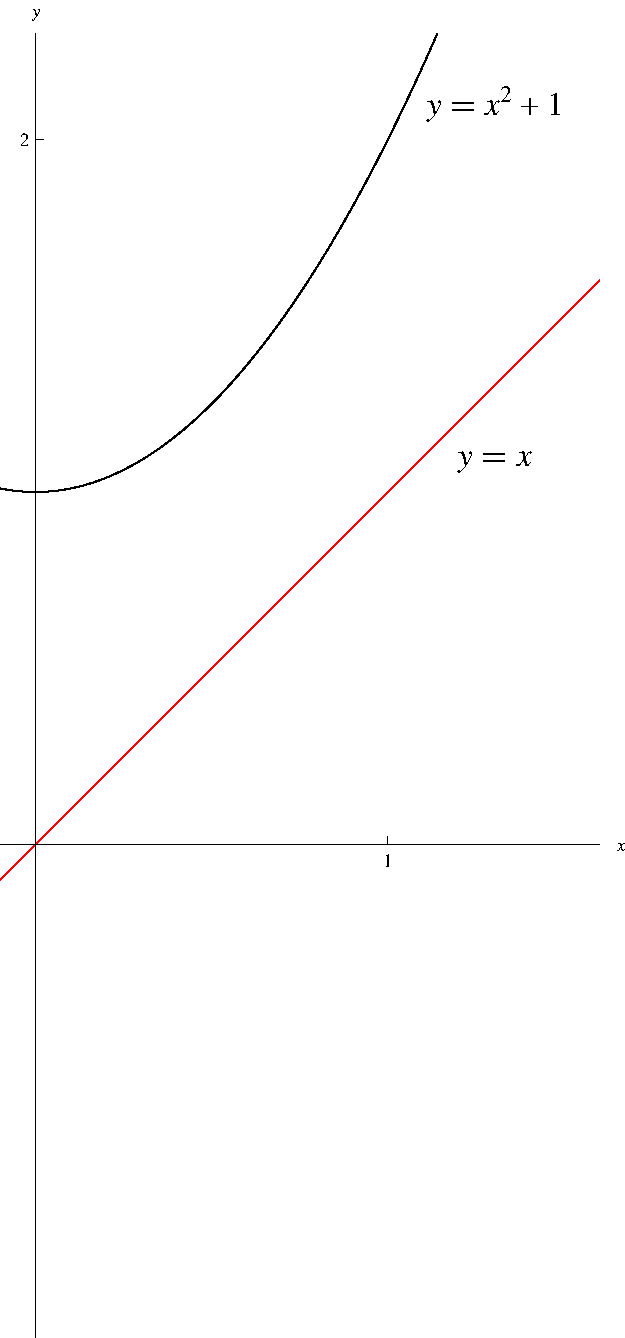
\includegraphics[height=3.3cm]{volumes/pictures/06-02-washerc.pdf} %
}%
\only<handout:0| 4>{%
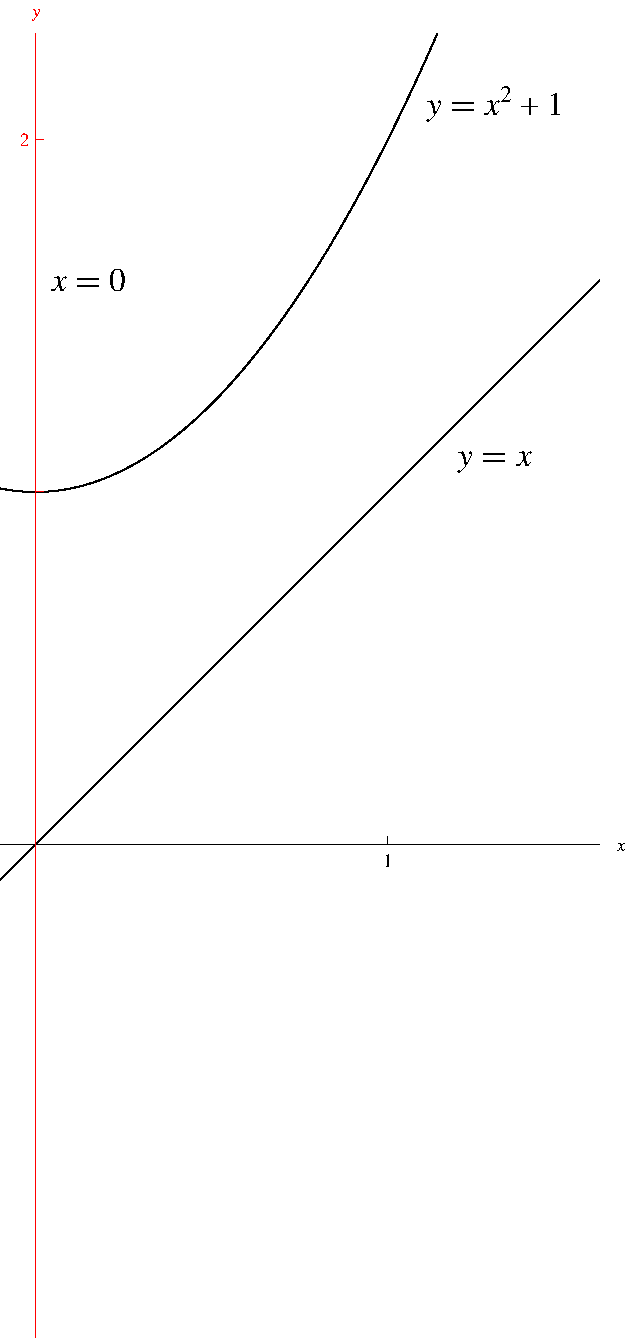
\includegraphics[height=3.3cm]{volumes/pictures/06-02-washerd.pdf} %
}%
\only<handout:0| 5>{%
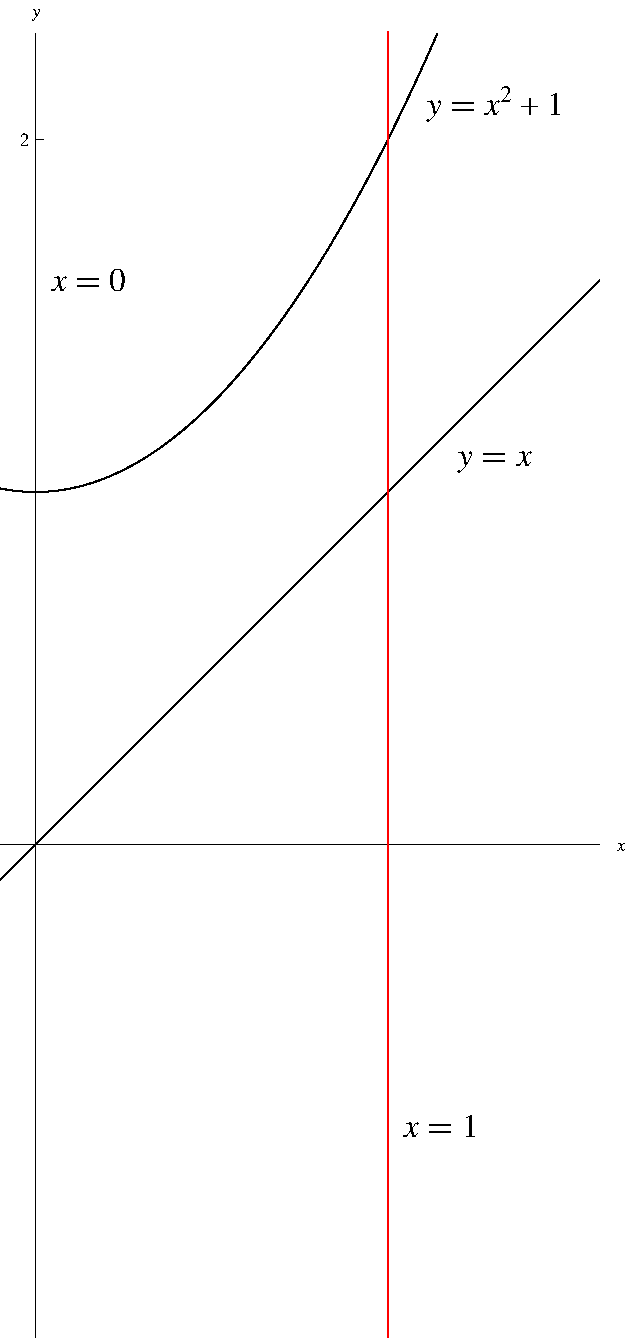
\includegraphics[height=3.3cm]{volumes/pictures/06-02-washere.pdf} %
}%
\only<handout:0| 6>{%
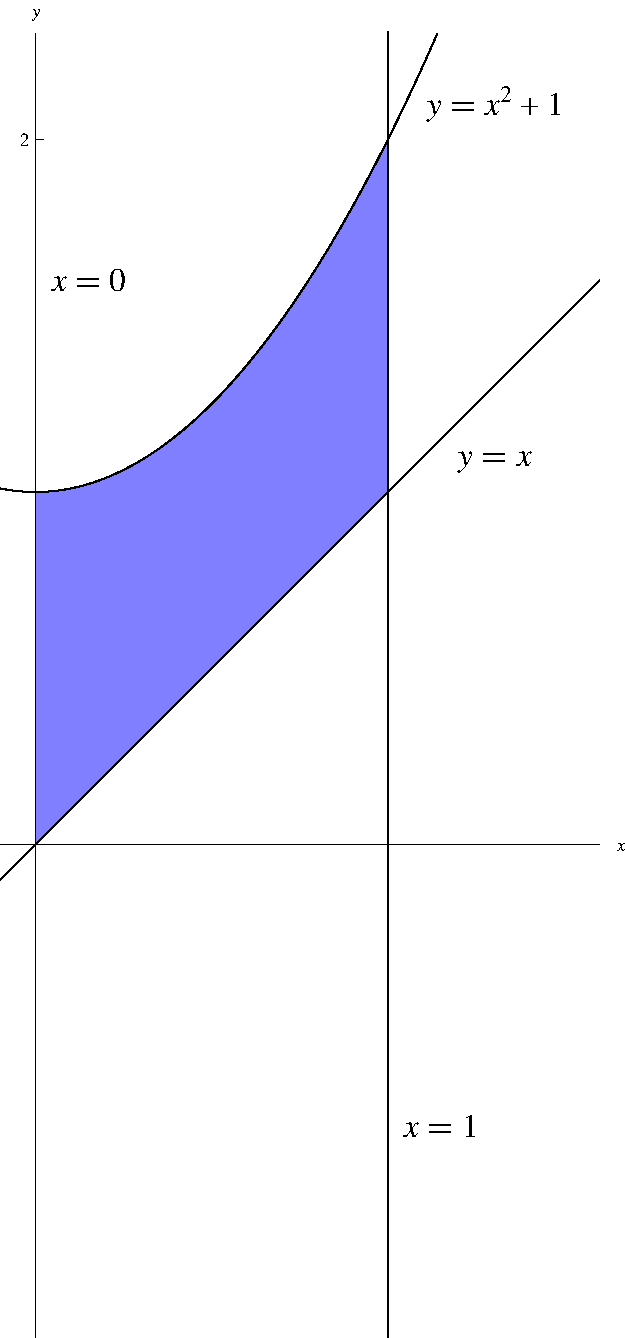
\includegraphics[height=3.3cm]{volumes/pictures/06-02-washerf.pdf} %
}%
\only<7->{%
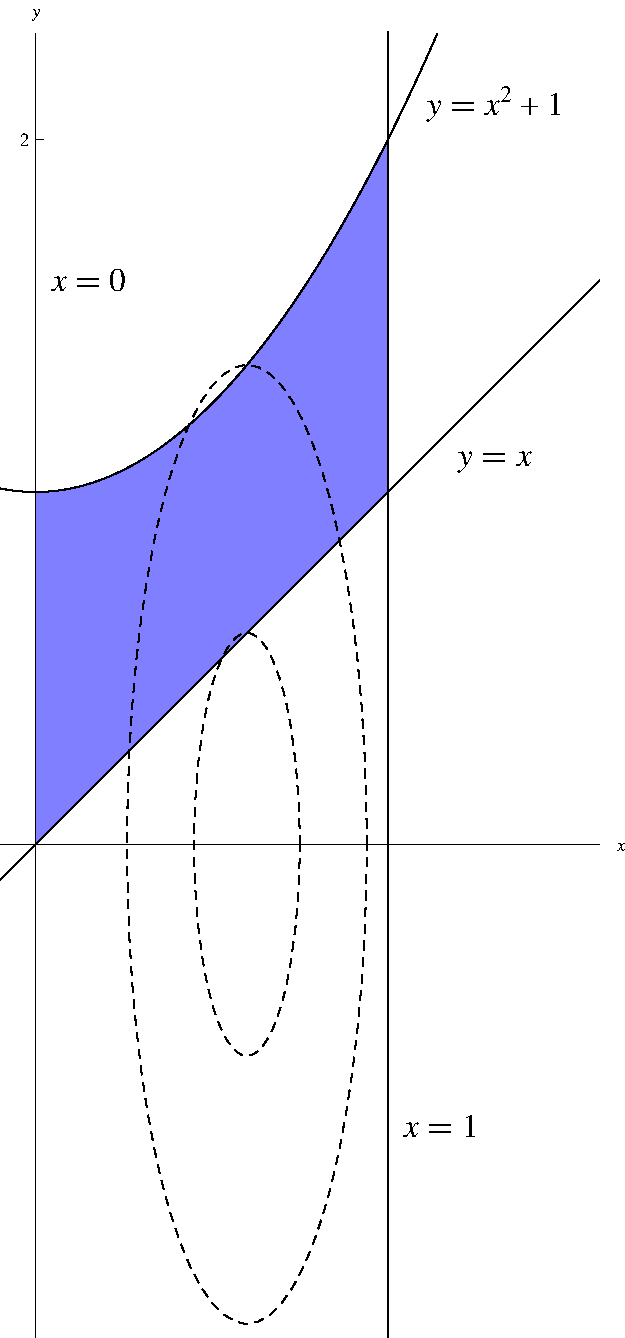
\includegraphics[height=3.3cm]{volumes/pictures/06-02-washerg.pdf} %
}%

\column{.65\textwidth}
Find the volume of the solid obtained by rotating about the $x$-axis \alert<handout:0| 6>{the region bounded by \alert<handout:0| 2>{$y = x^2+1$}, \alert<handout:0| 3>{$y = x$}, \alert<handout:0| 4>{$x = 0$}, and \alert<handout:0| 5>{$x = 1$}}.

\uncover<7->{%
The typical cross-section is a washer centered at $(x, 0)$.
}%

\uncover<8->{%
\alert<handout:0| 8-9>{Area of the inner circle: \uncover<9->{$\pi x^2$}}

\alert<handout:0| 10-11>{Area of the outer circle: \uncover<11->{$\pi (x^2+1)^2$}}
}%
\abovedisplayskip=0pt
\belowdisplayskip=0pt
\abovedisplayshortskip=0pt
\belowdisplayshortskip=0pt
\begin{align*}
\uncover<12->{%
V%
}%
& \uncover<12->{ = } %
\uncover<12->{%
\int_0^1 \left( \pi (x^2+1)^2 - \pi x^2    \right) \ \diff x%
}\\%
& \uncover<13->{ = } %
\uncover<13->{%
\pi \int_0^1 \left( \alert<handout:0| 14-15>{x^4} + \alert<handout:0| 16-17>{x^2} + \alert<handout:0| 18-19>{1} \right) \  \diff x%
}\\%
& \uncover<14->{ = } %
\uncover<14->{%
\pi \left[ \alert<handout:0| 15>{\uncover<15->{\frac{x^5}{5}}} + \alert<handout:0| 17>{\uncover<17->{\frac{x^3}{3}}} + \alert<handout:0| 19>{\uncover<19->{x}} \right]_0^1%
}\\%
& \uncover<20->{ = } %
\uncover<20->{%
\pi \left( \frac{1}{5} + \frac{1}{3} + 1\right) \uncover<21->{= \frac{23}{15}\pi}
}%
\end{align*}
\end{columns}
\end{example}
\end{frame}
% end module volumes-washer

% begin module volumes-otherline
\begin{frame}
\begin{example}[Rotated About a Line Other Than the $x$-axis]
Find the volume of the solid obtained by rotating about the line $y = 1$ \alert<handout:0| 4>{the region bounded by \alert<handout:0| 2>{$y = -x^2+2x+1$} and \alert<handout:0| 3>{$y = 1$}.}

\uncover<5->{%
The typical cross-section is a circle centered at $(x, 1)$.
}%

\uncover<6->{%
\alert<handout:0| 6-7>{Area of cross-section: \uncover<7->{$\pi ((-x^2+2x+1)-1)^2$}}
}%
\begin{columns}[c]
\column{.4\textwidth}
\begin{center}
\only<handout:0| 1>{%
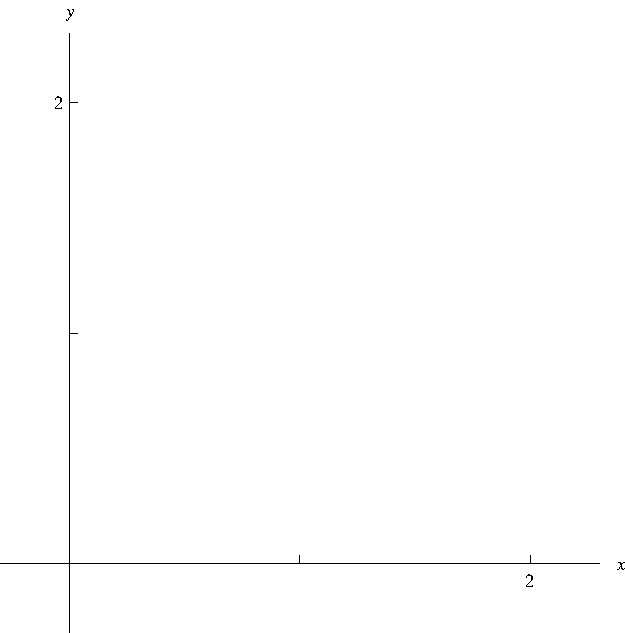
\includegraphics[height=5cm]{volumes/pictures/06-02-otherlinea.pdf} %
}%
\only<handout:0| 2>{%
\includegraphics[height=5cm]{volumes/pictures/06-02-otherlineb.pdf} %
}%
\only<handout:0| 3>{%
\includegraphics[height=5cm]{volumes/pictures/06-02-otherlinec.pdf} %
}%
\only<handout:0| 4>{%
\includegraphics[height=5cm]{volumes/pictures/06-02-otherlined.pdf} %
}%
\only<5->{%
\includegraphics[height=5cm]{volumes/pictures/06-02-otherlinee.pdf} %
}%
\end{center}
\column{.6\textwidth}

\abovedisplayskip=0pt
\belowdisplayskip=0pt
\begin{eqnarray*}
\uncover<8->{%
V%
}%
& \uncover<8->{ = } &%
\uncover<8->{%
\int_0^2  \pi \left( (-x^2+2x+1) -  1\right)^2  \ \diff x%
}\\%
& \uncover<9->{ = } &%
\uncover<9->{%
\pi \int_0^2 \left( \alert<handout:0| 10-11>{x^4} - \alert<handout:0| 12-13>{4x^3} + \alert<handout:0| 14-15>{4x^2} \right) \  \diff x%
}\\%
& \uncover<10->{ = } &%
\uncover<10->{%
\pi \left[ \alert<handout:0| 11>{\uncover<11->{\frac{x^5}{5}}} - \alert<handout:0| 13>{\uncover<13->{x^4}} + \alert<handout:0| 15>{\uncover<15->{\frac{4x^3}{3}}} \right]_0^2%
}\\%
& \uncover<16->{ = } &%
\uncover<16->{%
\pi \left( \frac{32}{5} - 16 + \frac{32}{3} \right) \uncover<17->{= \frac{16}{15}\pi}
}%
\end{eqnarray*}
\end{columns}
\end{example}
\end{frame}
% end module volumes-otherline

% end lecture

% begin lecture
\lect{September 12, 2011}{Lecture 2}{2}
\section{(6.3) Volumes by Cylindrical Shells}
% begin module cylindrical-shells-intro
\begin{frame}[t]
Find the volume obtained by rotating the region bounded by \alertNoH{2}{$ y = 2x^2 - x^3$} and the \alertNoH{3}{$x$-axis} around $\ldots$
\begin{columns}
\column{0.5\textwidth}
\begin{pspicture}(-2.2,-1.2)(2.5,2.3)%
\tiny%
\renewcommand{\fcScreenStyle}{x}%
\fcBoundingBox{-2.2}{-1.2}{2.5}{2.3}%
\renewcommand{\fcScreen}{[0 0 -1] 0}%
\renewcommand{\fcIterationsU}{4}%
\only<handout:2|5->{\renewcommand{\fcScreen}{[-0.07 dup -1] 0}}%
\only<handout:2|6->{\renewcommand{\fcScreen}{[-0.14 dup -1] 0}}%
\only<handout:2|7->{\renewcommand{\fcScreen}{[-0.21 dup -1] 0}}%
\only<handout:2,3|8->{\renewcommand{\fcScreen}{[-0.28 dup -1] 0}}%
\newcommand{\theFun}{u u mul 2 mul u u u mul mul sub\space}%
\newcommand{\theYAxis}{0\space}%
\newcommand{\theSurfaceFla}{u v cos \theFun mul v sin \theFun mul\space}%
\newcommand{\theSurface}{%
\fcSurfaceInScene[colorVU= {1 0.5 0.5}, iterationsU=6, arrows=none, linewidth=0.3, linecolor=black, forceForeground=true]{0.03}{0}{1.99}{30 \fcIterationsV\space mul}{[\theSurfaceFla]}{}%
}%
\uncover<handout:1|4-8>{\pscustom*[linecolor=\fcColorAreaUnderGraph]{%
\fcLineIIId{ [0 0 0]}{[2 0  0]}%
\fcCurveIIId{2}{0}{[1 dict begin /u t def t \theFun 0 end]}%
}}%
\fcStartIIIdScene%
\fcAxesIIIdFullInScene[linewidth=1, linecolor=black, arrows=->, xLabel={$x$}, yLabel={$y$},zLabel={} ]{-0.5}{-1.2}{-3}{2.2}{2.2}{3}%
\uncover<handout:2,3|8->{\fcPutIIId[t]{[0 0 3.1]}{$z$}}%
\only<handout:0|9>{%
\renewcommand{\fcIterationsV}{4}%
\theSurface%
}%
\only<handout:0|10>{%
\renewcommand{\fcIterationsV}{8}%
\theSurface%
}%
\only<handout:2|11,12>{%
\renewcommand{\fcIterationsV}{12}%
\theSurface%
}%
\only<handout:2,3|12->{%
\fcSurfaceInScene[linewidth=1, arrows=(none), colorUV=cyan, colorVU=cyan, linecolor=blue, iterationsU=12, iterationsV=1, forceForeground=false]{0}{0.9}{360}{1}{1 dict begin /theRadius 1 dict begin /u 0.9 def \theFun end def [ v u cos  theRadius mul u sin theRadius mul] end}{}%
\fcSurfaceInScene[linewidth=1, arrows=(none), colorUV=cyan, colorVU=cyan, linecolor=blue, iterationsU=12, iterationsV=1, forceForeground=false]{0}{0.01}{360}{1 dict begin /u 0.9 def \theFun  end}{[1 u cos v mul  u sin v mul ]}{}%
\fcSurfaceInScene[linewidth=1, arrows=(none), colorUV=cyan, colorVU=cyan, linecolor=blue, iterationsU=12, iterationsV=1, forceForeground=false]{0}{0.8}{360}{1 dict begin /u 0.9 def \theFun  end}{[0.9 u cos v mul u sin v mul ]}{}%
}%
\only<4->{\fcCurveIIIdInScene[linewidth=1, arrows=(none), linecolor= \fcColorGraph]{0}{2}{1 dict begin /u {t} def  [t \theFun 0] end}}%
\only<4->{\fcLineIIIdInScene[linewidth=1, arrows=(none), linecolor= \fcColorGraph]{[0 0 0]}{[2 0 0]}}%
\fcFinishIIIdScene%
\only<handout:1|2-3>{\fcCurveIIId{-0.8}{2.2}{1 dict begin /u {t} def  [t \theFun 0] end}}%
\only<handout:1|3>{\fcLineIIId[linecolor=\fcColorGraph]{[-0.8 0 0]}{[2.1 0 0]}}%
\uncover<handout:3|13->{ \fcLineIIId[linecolor=black, linewidth=0.4pt]{[0.9 -0.05 0]}{[0.9 0.05 0]}}%
\fcLineIIId[linecolor=black, linewidth=0.4pt]{[2 -0.05 0]}{[2 0.05 0]}%
\fcLineIIId[linecolor=black, linewidth=0.4pt]{[-0.05 1 0]}{[0.05 1 0]}%
\uncover<handout:3|13->{ \fcPutIIId[t]{[1 -0.1 0]}{$x$}}%
\fcPutIIId[t]{[2 -0.1 0]}{$2$}%
\fcPutIIId[r]{[-0.1 1 0]}{$1$}%
\only<2->{\fcPutIIId[b]{[4 3 div 1.5 0]}{$\alertNoH{2}{y=2x^2-x^3}$}}%
%\only<handout:0|25->{%
%\fcLineIIId[linecolor=blue, linewidth=2pt]{[0 0 0]}{[2 0 0]}%
%\fcDotIIId[linecolor=blue]{[0 0 0]}
%\fcDotIIId[linecolor=blue]{[2 0 0]}
%}%
\end{pspicture}

\vskip -0.3cm
\begin{itemize}
\item<1->  \alertNoH{9-12}{ $\ldots$ the $x$-axis.}
\item<13->  Approximate the volume using circular cylinders with radius $2x^2 - x^3$ and height $\Delta x$.
\item<14->  $V = \int_0^2 \pi (2x^2 - x^3)^2 \diff x$.
\item<15->  We understand the problem.
\end{itemize}
\vskip 5cm


\column{0.5\textwidth}
\begin{pspicture}(-2.3,-1.15)(2.5,2.4)%
\tiny%
\renewcommand{\fcScreenStyle}{x}%
\fcBoundingBox{-2.3}{-1.15}{2.5}{2.4}%
\renewcommand{\fcScreen}{[0 0 -1] 0}%
\renewcommand{\fcIterationsU}{4}%
\only<handout:2|5->{\renewcommand{\fcScreen}{[-0.07 dup -1] 0}}%
\only<handout:2|6->{\renewcommand{\fcScreen}{[-0.14 dup -1] 0}}%
\only<handout:2|7->{\renewcommand{\fcScreen}{[-0.21 dup -1] 0}}%
\only<handout:2,3|8->{\renewcommand{\fcScreen}{[-0.28 dup -1] 0}}%
\newcommand{\theFun}{u u mul 2 mul u u u mul mul sub\space}%
\newcommand{\theYAxis}{0\space}%
\newcommand{\theSurfaceFla}{v cos u mul \theFun v sin u mul\space}%
\newcommand{\theSurface}{%
\fcSurfaceInScene[colorVU= {1 0.5 0.5}, iterationsU=6, arrows=none, linewidth=0.3, linecolor=black, forceForeground=true ]{0.03}{0}{1.99}{30 \fcIterationsV\space mul}{[\theSurfaceFla]}{}%
}%
\uncover<handout:1|4-16,24->{\pscustom*[linecolor=\fcColorAreaUnderGraph]{%
\fcLineIIId{ [0 0 0]}{[2 0  0]}%
\fcCurveIIId{2}{0}{[1 dict begin /u t def t \theFun 0 end]}%
}}%
\fcStartIIIdScene%
\fcAxesIIIdFullInScene[linewidth=1, linecolor=black, arrows=->, xLabel={$x$}, yLabel={$y$},zLabel={} ]{-2.3}{-0.5}{-3.2}{2.3}{2.3}{3.2}%
%\fcAxesIIIdInScene[zLabel={}, arrows=->]{2.2}{2.2}{3}%
\uncover<handout:2,3|8->{\fcPutIIId[t]{[0 0 3.1]}{$z$}}%
\only<handout:0|17>{%
\renewcommand{\fcIterationsV}{4}%
\theSurface%
}%
\only<handout:0|18>{%
\renewcommand{\fcIterationsV}{8}%
\theSurface%
}%
\only<handout:2|19,20>{%
\renewcommand{\fcIterationsV}{12}%
\theSurface%
}%
\only<handout:2,3|20-23>{%
\fcSurfaceInScene[linewidth=1, arrows=(none), colorUV=cyan, colorVU=cyan, linecolor=blue, iterationsU=12, iterationsV=1, forceForeground=false]{0}{0.9}{360}{1}{[u cos 5 sqrt 1 add 2 div mul v u sin 5 sqrt 1 add 2 div mul]}{}%
\fcSurfaceInScene[linewidth=1, arrows=(none), colorUV=cyan, colorVU=cyan, linecolor=blue, iterationsU=12, iterationsV=1, forceForeground=false]{0}{0.9}{360}{1}{[u cos v u sin ]}{}%
\fcSurfaceInScene[linewidth=1, arrows=(none), colorUV=cyan, colorVU=cyan, linecolor=blue, iterationsU=12, iterationsV=1, forceForeground=false]{0}{1}{360}{5 sqrt 1 add 2 div}{[u cos v mul 1 u sin v mul ]}{}%
}%
\only<4->{\fcCurveIIIdInScene[linewidth=1, arrows=(none), linecolor= \fcColorGraph]{0}{2}{1 dict begin /u {t} def  [t \theFun 0] end\space}}%
\only<4->{\fcLineIIIdInScene[linewidth=1, arrows=(none), linecolor= \fcColorGraph]{[0 0 0]}{[2 0 0]}}%
\fcFinishIIIdScene%
\only<handout:1|2-3>{\fcCurveIIId{-0.8}{2.2}{1 dict begin /u {t} def  [t \theFun 0] end}}%
\only<handout:1|3>{\fcLineIIId[linecolor=\fcColorGraph]{[-0.8 0 0]}{[2.1 0 0]}}%
\fcLineIIId[linecolor=black, linewidth=0.4pt]{[-0.05 1 0]}{[0.05 1 0]}%
\fcLineIIId[linecolor=black, linewidth=0.4pt]{[2 -0.05 0]}{[2 0.05 0]}%
\uncover<handout:4|24->{\fcLineIIId[linecolor=black, linewidth=0.4pt]{[1 -0.05 0]}{[1 0.05 0]}%
\fcLineIIId[linecolor=black, linewidth=0.4pt]{[5 sqrt 1 add 2 div -0.05 0]}{[5 sqrt 1 add 2 div 0.05 0]}%
\fcLineIIId[linecolor=black, linestyle=dotted, linewidth=0.4pt]{[5 sqrt 1 add 2 div 0 0]}{[5 sqrt 1 add 2 div 1 0]}%
\fcLineIIId[linecolor=black, linestyle=dotted, linewidth=0.4pt]{[1 0 0]}{[1 1 0]}%
\uncover<handout:3|21->{ \fcPutIIId[t]{[1 -0.1 0]}{$x_i$}}%
\uncover<handout:3|21->{ \fcPutIIId[t]{[5 sqrt 1 add 2 div -0.1 0]}{$x_o$}}%
}%
\uncover<handout:3|21->{ \fcPutIIId[r]{[-0.1 1 0]}{$y$}}%
\fcPutIIId[t]{[2 -0.1 0]}{$2$}%
\only<2->{\fcPutIIId[b]{[4 3 div 1.5 0]}{$\alertNoH{2,24}{y=2x^2-x^3}$}}%
\uncover<handout:0|23>{\fcLineIIId[linecolor=purple, linewidth=2.2pt]{[0 1 0]}{[5 sqrt 1 add 2 div 1 0]}}%
\uncover<handout:0|22,23>{\fcLineIIId[linecolor=red, linewidth=1.8pt]{[0 1 0]}{[1 1 0]}}%
\uncover<handout:4|24->{\fcLineIIId[linecolor=purple, linewidth=1.2pt]{[0 1 0]}{[5 sqrt 1 add 2 div 1 0]}%
\fcLineIIId[linecolor=red, linewidth=1pt]{[0 1 0]}{[1 1 0]}%
}%
\end{pspicture}

\begin{itemize}
\item<1-> \alertNoH{16-19}{ $\ldots$ the $y$-axis.}
\item<21-> Approx. with washers: \uncover<22->{need \alertNoH{22}{inner rad. $x_i$}} \uncover<23->{\& \alertNoH{23}{outer rad. $x_o$}}.
\item<handout:4|24-> $x_i$ and $x_o$: solutions to cubic: $\alertNoH{24}{-x^3+2x^2-y=0} $. \uncover<25->{Solving for $x$ requires lots of algebra.} 
\item<handout:4|26->  We show a simpler technique.
\end{itemize}

\end{columns}
\vskip 5cm
\end{frame}
% end module cylindrical-shells-intro

\begin{frame}
\begin{tabular}{cc}
\psset{xunit=0.75cm, yunit=0.75cm}
\begin{pspicture}(-3,-3)(3,3)
\renewcommand{\fcScreen}{[-1 -1 -1] 0}
%\pscustom*[linecolor=cyan]{%
%\fcPolyLineIIId{[-2 -2 0] [-2 2 0] [2 2 0] [2 -2 0] [-2 -2 0]}%
%}%
\pscustom*[linecolor=white]{%
\fcCurveIIId{0}{360}{[2 t cos mul 2 t sin mul 0]}%
}%
%\fcAxesIIId{2}{2}{2}
\fcBoxIIId[linecolor=gray!30, linewidth=0.3pt]{[2 2 2]}{[2 2 0]}{[2 -2 2]}{[-2 2 2]}%
\fcPlotIIIdXconst[linewidth=0.3pt, linecolor=\fcColorGraph]{iterationsX=15, iterationsY=15}{-2}{4 x x mul sub sqrt -1 mul}{2}{4 x x mul sub sqrt}{1 dict begin /rho x x mul y y mul  add sqrt def rho rho mul 2 rho  sub mul  0 max end}%
\fcPlotIIIdYconst[linewidth=0.3pt, linecolor=\fcColorGraph]{iterationsX=10, iterationsY=10}{4 y y mul sub sqrt -1 mul}{-2}{4 y y mul sub sqrt}{2}{1 dict begin /rho x x mul y y mul  add sqrt def rho rho mul 2 rho  sub mul  0 max end}%
\fcCurveIIId[linecolor=\fcColorGraph]{0}{360}{[2 t cos mul 2 t sin mul 0]}%
\end{pspicture}

%\includegraphics[height=4cm]{volumes/pictures/06-03-setup3d.pdf}%
&%
\psset{xunit=0.75cm, yunit=0.75cm}
\begin{pspicture}(-3,-3)(3,3)
\tiny%
\renewcommand{\fcScreen}{[-1 -1 -1] 0}%
\newcommand{\numIterations}{20\space}%
\pstVerb{%
100 dict begin
/numIterations \numIterations\space def
/goodAngleMin -50 def
/goodAngleMax 140 def
}%
\newcommand{\FunFla}{x x mul 2 mul x x x mul mul sub\space}%
\newcommand{\widthLine}{0.2pt}%
%\pscustom*[linecolor=cyan]{%
%\fcPolyLineIIId{[-2 -2 0] [-2 2 0] [2 2 0] [2 -2 0] [-2 -2 0]}%
%}%
%\pscustom*[linecolor=white]{%
%\fcCurveIIId{0}{360}{[2 t cos mul 2 t sin mul 0]}%
%}%
%\fcAxesIIId{2}{2}{2}%
%\fcStartIIIdScene%
%\fcSurfaceDirectDraw{}{}{}{}{}{}
%\fcFinishIIIdScene[true]%
\pstVerb{20 dict begin}%
\multido{\na=0+1}{\numIterations}{%
\pstVerb{%
/theCounter numIterations \na\space sub 1 sub def%
/theRad theCounter numIterations div 2 mul def
/theRadNext theCounter 1 add numIterations div 2 mul def
1 dict begin /x theRad def \FunFla end 
/theHeight exch def
1 dict begin /x theRadNext def \FunFla end 
/theHeightNext exch def
}%
%\pscustom*[linecolor=white]{%
%\fcCurveIIId{goodAngleMin 360 add}{goodAngleMax}{  [t cos theRad mul t sin theRad mul theHeight] }%
%\fcLineIIId{[goodAngleMax cos theRad mul goodAngleMax sin theRad mul theHeight]}{[goodAngleMax cos theRad mul goodAngleMax sin theRad mul theHeightNext]}%
%\fcCurveIIId{goodAngleMax}{goodAngleMin 360 add}{  [t cos theRad mul t sin theRad mul theHeightNext] }%
%\fcLineIIId{[goodAngleMin cos theRad mul goodAngleMin sin theRad mul theHeightNext]}{[goodAngleMin cos theRad mul goodAngleMin sin theRad mul theHeight]}%
%}%
\fcCurveIIId[linecolor=red, linewidth=\widthLine]{goodAngleMin 360 add}{goodAngleMax}{  [t cos theRad mul t sin theRad mul theHeight] }%
%\fcLineIIId[linecolor=\fcColorGraph]{[goodAngleMax cos theRad mul goodAngleMax sin theRad mul theHeight]}{[goodAngleMax cos theRad mul goodAngleMax sin theRad mul theHeightNext]}%
\fcCurveIIId[linecolor=red, linewidth=\widthLine]{goodAngleMin 360 add }{goodAngleMax}{  [t cos theRad mul t sin theRad mul theHeightNext] }%
%\fcLineIIId[linecolor=\fcColorGraph]{[goodAngleMin cos theRad mul goodAngleMin sin theRad mul theHeightNext]}{[goodAngleMin cos theRad mul goodAngleMin sin theRad mul theHeight]}%
}%
\multido{\nb=0+1}{\numIterations}{%
\pstVerb{%
/theCounter \nb\space def%
/theRad theCounter numIterations div 2 mul def
/theRadNext theCounter 1 add numIterations div 2 mul def
1 dict begin /x theRad def \FunFla end 
/theHeight exch def
1 dict begin /x theRadNext def \FunFla end 
/theHeightNext exch def
}%
%\pscustom*[linecolor=white]{%
%\fcCurveIIId{goodAngleMin}{goodAngleMax}{  [t cos theRad mul t sin theRad mul theHeight] }%
%\fcLineIIId{[goodAngleMax cos theRad mul goodAngleMax sin theRad mul theHeight]}{[goodAngleMax cos theRad mul goodAngleMax sin theRad mul theHeightNext]}%
%\fcCurveIIId{goodAngleMax}{goodAngleMin}{[t cos theRad mul t sin theRad mul theHeightNext]}%
%\fcLineIIId{    [goodAngleMin cos theRad mul goodAngleMin sin theRad mul theHeightNext]}{[goodAngleMin cos theRad mul goodAngleMin sin theRad mul theHeight]}%
%}%
\fcCurveIIId[linecolor=red, linewidth=\widthLine]{goodAngleMin }{goodAngleMax}{  [t cos theRad mul t sin theRad mul theHeight] }%
%\fcLineIIId[linecolor=\fcColorGraph, linewidth=0.4pt]{[goodAngleMax cos theRad mul goodAngleMax sin theRad mul theHeight]}{[goodAngleMax cos theRad mul goodAngleMax sin theRad mul theHeightNext]}%
\fcCurveIIId[linecolor=red, linewidth=\widthLine]{goodAngleMax }{goodAngleMin}{  [t cos theRad mul t sin theRad mul theHeightNext] }%
%\fcLineIIId[linecolor=\fcColorGraph, linewidth=0.2pt]{[goodAngleMin cos theRad mul goodAngleMin sin theRad mul theHeightNext]}{[goodAngleMin cos theRad mul goodAngleMin sin theRad mul theHeight]}%
}%
\pstVerb{end}%
\fcBoxIIId[linewidth=0.2pt, linecolor=gray!30]{[2 2 2]}{[2 2 0]}{[2 -2 2]}{[-2 2 2]}%
\fcCurveIIId[linecolor=\fcColorGraph]{0}{360}{[2 t cos mul 2 t sin mul 0]}%
\pstVerb{end}%
\end{pspicture}
%\includegraphics[height=4cm]{volumes/pictures/06-03-setupcylinders.pdf}%
\end{tabular}
\begin{itemize}
\item<1->  Consider the solid obtained by rotating around the $y$-axis the region bounded above by $y = 2x^2 - x^3$ and below by the $x$-axis.
\item<2->  Approximate this solid by nested cylindrical shells.
\item<3->  Cylindrical shells are solids obtained by taking a cylinder and removing from its center another cylinder of equal height but smaller radius.
\end{itemize}
\end{frame}\begin{frame}
\begin{columns}
\column{0.3\textwidth}
\begin{pspicture}(-1.4,-1.4)(1.4,1.4)
\tiny
\pstVerb{100 dict begin /innerRad 1 def /outerRad 1.4 def}%
\fcStartIIIdScene
\fcSurfaceInScene[colorUV={0.8 0.9 1}, colorVU={0.7 0.7 1}, linewidth=0.4, iterationsU=17, iterationsV=1]{0 }{-1}{360}{1}{[u cos innerRad mul u sin innerRad mul v]}{}
\fcSurfaceInScene[colorUV={0.8 0.9 1}, colorVU={0.7 0.7 1}, iterationsU=17, iterationsV=1]{0 }{-1}{360}{1}{[u cos outerRad mul u sin outerRad mul v]}{}
\fcSurfaceInScene[colorUV={0.8 0.9 1}, colorVU={0.8 0.9 1}, iteraionsU=17, iterationsV=1]{0 }{innerRad}{ 360}{ outerRad }{[u cos v mul u sin v mul 1]}{}
\fcSurfaceInScene[colorUV={0.8 0.9 1}, colorVU={0.7 0.7 1}, iteraionsU=17, iterationsV=1]{0 }{innerRad}{ 360}{ outerRad }{[u cos v mul u sin v mul -1]}{}
\fcFinishIIIdScene[true]%
\only<2->{%
\fcLineIIId[linecolor=red, linewidth=2pt]{[0 0 1]}{[-720 17 div cos outerRad mul -720 17 div sin outerRad mul 1]}%
\fcPutIIId{[0 -0.3 0.9]}{$\alertNoH{2}{r_2}$}%
}%
\only<3->{%
\fcLineIIId[linecolor=red, linewidth=2pt]{[0 0 1]}{[0 cos innerRad mul 0 sin innerRad mul 1]}%
\fcPutIIId{[0.5 0 1.2]}{$\alertNoH{3}{r_1}$}%
}%
\only<4->{%
\fcLineIIId[linecolor=red, linewidth=2pt]{[360 17 div cos outerRad mul 360 17 div sin outerRad mul -1]}{[360 17 div cos outerRad mul 360 17 div sin outerRad mul 1]}%
\fcPutIIId{[360 17 div cos outerRad mul 360 17 div sin outerRad mul -1.2]}{$\alertNoH{4}{h}$}%
}%
\only<9->{% 
\fcLineIIId[linecolor=red, linewidth=2pt]{[-360 17 div cos outerRad mul -360 17 div sin outerRad mul 1]}{[-360 17 div cos innerRad mul -360 17 div sin innerRad mul 1]}%
\fcPutIIId{[1.4 -0.5 0.85]}{$\alertNoH{9}{\Delta r}$}%
}%
\only<10->{% 
\fcLineIIId[linecolor=red, linewidth=2pt]{[360 17 div 5.5 mul cos innerRad outerRad add 2 div mul 360 17 div 5.5 mul sin innerRad outerRad add 2 div mul 1]}{[0 0 1]}%
\fcPutIIId{[-0.5 1.4 1]}{$\alertNoH{10}{r}$}%
}
\pstVerb{end}%
\end{pspicture}
%the graphics here looks better:
%\ \includegraphics[height=4cm]{volumes/pictures/06-03-cylinder.pdf}%
%however I prefer to stay with internal graphics for the purposes of highlighting and uncovering things. 
%It should be possible to modify the internal 3d graphics to make it look as good as the original...
\column{0.7\textwidth}
\begin{itemize}
\item<1->  Consider a cylindrical shell with:
\item<2->  \alertNoH{2}{outer radius $r_2$},
\item<3->  \alertNoH{3}{inner radius $r_1$},
\item<4->  \alertNoH{4}{height $h$}.
\item<5->  $V_{\text{shell}} = \alertNoH{6}{V_{\text{outer cyl.}}} - \alertNoH{7}{V_{\text{inner cyl.}}} \uncover<6->{= \alertNoH{6}{ \pi \alertNoH{8}{r_2^2} h} - \alertNoH{7}{\pi \alertNoH{8}{r_1^2} h} } \uncover<8->{ = \alertNoH{11}{\pi} \alertNoH{8}{(\alertNoH{14}{r_2 - r_1})(\alertNoH{12}{r_2 + r_1})}\alertNoH{13}{h}}$.
\item<9->  Let $\alertNoH{9}{\Delta r = r_2 - r_1}$.
\item<10->  Let $\displaystyle r = \frac{r_2+r_1}{2}$.
\item<11->  Then $V_{\text{shell}} = \alertNoH{12}{2} \alertNoH{11}{ \pi} \alertNoH{12}{r}\alertNoH{13}{h}\alertNoH{14}{\Delta r}$.
\end{itemize}
\end{columns}
\end{frame}
\begin{frame}
\begin{columns}
\column{0.35\textwidth}
\begin{pspicture}(-1,-2)(3,3)%
\tiny%
\renewcommand{\fcScreenStyle}{x}%
\fcBoundingBox{-2.2}{-1.1}{2.5}{2.4}%
\renewcommand{\fcScreen}{[0 0 -1] 0}%
\renewcommand{\fcScreen}{[-0.28 dup -1] 0}%
\newcommand{\theFun}{x x mul 2 mul x x x mul mul sub\space}%
\newcommand{\theYAxis}{0\space}%
\newcommand{\theSurfaceFla}{1 dict begin /x u def v cos u mul \theFun v sin u mul end\space}%
\fcStartIIIdScene%
\fcAxesIIIdInScene[zLabel={}, arrows=->]{2.2}{2.2}{3}%
\fcPutIIId[t]{[0 0 3.1]}{$z$}%
\only<handout:1|1,2>{%
\fcSurfaceInScene[colorVU= {1 0.5 0.5}, iterationsU=6, iterationsV=12, arrows=none, linewidth=0.3, linecolor=black, forceForeground=true ]{0.03}{0}{2}{360}{[\theSurfaceFla]}{}%
}%
\fcCurveIIIdInScene[linewidth=1, arrows=(none), linecolor= \fcColorGraph]{0}{2}{1 dict begin /x {t} def  [t \theFun 0] end\space}%
\fcFinishIIIdScene%
%\fcCurveIIId{-0.8}{2.2}{1 dict begin /u {t} def  [t \theFun 0] end}%
%\fcLineIIId[linecolor=black, linewidth=0.4pt]{[-0.05 1 0]}{[0.05 1 0]}%
%\fcLineIIId[linecolor=black, linewidth=0.4pt]{[1 -0.05 0]}{[1 0.05 0]}%
\newcommand{\numIterations}{5}%
\only<handout:0|10->{\renewcommand{\numIterations}{10}}%
\only<handout:0|11->{\renewcommand{\numIterations}{15}}%
\only<handout:0|12->{\renewcommand{\numIterations}{20}}%
\only<handout:2|2->{%
\multido{\na=1+1}{\numIterations}{%
\pstVerb{%
/numIterations \numIterations\space def
/theCounter \na\space 1 sub def%
/theRad theCounter numIterations div 2 mul def
/theRadNext theCounter 1 add numIterations div 2 mul def
/theRadNextNext theCounter 2 add numIterations div 2 mul def
1 dict begin /x theRad theRadNext add 2 div def \theFun end 
/theHeight exch def
1 dict begin /x theRadNext theRadNextNext add 2 div def \theFun end 
/theHeightNext exch def
/theHeightNext theHeightNext 0 lt {0}{theHeightNext}ifelse def
/goodAngleMax 160 def
/goodAngleMin -10 def
}%
\fcCurveIIId[linecolor=cyan, linewidth=0.3pt]{0}{360}{  [t cos theRad mul theHeight t sin theRad mul ] }%
%\fcCurveIIId[linecolor=red, linewidth=0.3pt]{0}{360}{  [t cos theRad mul 0 t sin theRad mul ] }%
\fcLineIIId[linecolor=cyan]{[goodAngleMax cos theRadNext mul theHeight goodAngleMax sin theRadNext mul]}{[goodAngleMax cos theRadNext mul theHeightNext goodAngleMax sin theRadNext mul ]}%
\fcCurveIIId[linecolor=cyan, linewidth=0.3pt]{0 }{360}{  [t cos theRadNext mul theHeight t sin theRadNext mul ] }%
\fcLineIIId[linecolor=cyan]{[goodAngleMin cos theRadNext mul theHeight goodAngleMin sin theRadNext mul]}{[goodAngleMin cos theRadNext mul theHeightNext goodAngleMin sin theRadNext mul ]}%
\only<-10>{%
\fcLineIIId[linecolor=black, linewidth=0.4pt]{[theRad -0.05 0]}{[ theRad  0.05 0]}%
\fcLineIIId[linecolor=black, linewidth=0.4pt]{[theRad theRadNext add 2 div -0.03 0  ]}{[theRad theRadNext add 2 div 0.03 0 ]}%
}%
%\fcCurveIIId[linecolor=red, linewidth=0.3pt]{0 }{360}{  [t cos theRadNext mul 0 t sin theRadNext mul ] }%
%\fcLineIIId[linecolor=\fcColorGraph]{[goodAngleMin cos theRad mul goodAngleMin sin theRad mul theHeightNext]}{[goodAngleMin cos theRad mul goodAngleMin sin theRad mul theHeight]}%
\only<5>{%
\fcLineIIId[linewidth=0.3pt]{[theRadNext theRad add 2 div 0 0]}{[theRadNext theRad add 2 div theHeight 0]}%
\fcLineIIId[linewidth=0.3pt]{[theRad theHeight 0]}{[theRadNext theHeight 0]}%
}%
\only<6-10>{\fcPutIIId[t]{[theRadNext theRad add 2 div -0.1 0]}{$x_{\na}$}}%
}%
\only<handout:0|5>{\fcLineIIId[linecolor=purple, linewidth=1.5pt]{[theRad theRadNext add 2 div 0 0]}{[theRad theRadNext add 2 div theHeight 0]}%
\fcPutIIId[t]{[theRad theRadNext add 2 div -0.1 0]}{$r$}%
}%
\fcCurveIIId[linecolor=cyan, linewidth=0.3pt]{0}{360}{[t cos 2 mul 0 t sin 2 mul]}%
\only<handout:0|14->{%
\fcLineIIId[linecolor=blue, linewidth=1.5pt]{[0 0 0]}{[2 0 0]}%
\fcDotIIId[linecolor=blue]{[0 0 0]}%
\fcDotIIId[linecolor=blue]{[2 0 0]}%
\fcPutIIId{[2 -0.1 0]}{$b$}
\fcPutIIId{[0 -0.1 0]}{$a$}
}%
}%only
\end{pspicture}
\column{0.65\textwidth}

Consider a solid obtained by rotating the region under $f(x)$ around the $y$ axis. \uncover<2->{ Approximate the volume by cylindrical shells.  \uncover<5->{Select the height of an individual shell to be $h = f(r)$ ($r$=average outer \& inner radius).}

\hfil \hfil $
\uncover<4->{ V_{\text{shell}} = 2\pi r \alertNoH{5}{h}\Delta r} \uncover<5->{ = 2\pi \alertNoH{7}{r} \alertNoH{5}{f(\alertNoH{7}{r})} \alertNoH{8}{\Delta r} .}
$
}
\end{columns}
\uncover<6->{
Suppose there are $n$ cyclindrical shells and let $x_1, \ldots , x_n$ be the averages of outer and inner radii. The shell volume sum is:

\hfil \hfil $\displaystyle
\sum_{i=1}^n 2\pi \alertNoH{7}{x_i} f(\alertNoH{7}{x_i})\alertNoH{8}{ \Delta x}.
$
}

\uncover<9->{
Take the limit as the number of shells goes to $\infty$ to get
\[
V = \lim_{n\to \infty} V_{\text{approx}}= \lim_{n\rightarrow\infty} \sum_{i=1}^n 2\pi x_i f(x_i)\Delta x \uncover<13->{= \int_{\alertNoH{ 14}{a}}^{\alertNoH{ 14}{b}}2\pi xf(x) \diff x .}
\]
\uncover<14->{
The endpoints of integration are the endpoints of the rotated region.
}
}
\end{frame}

\begin{frame}
\begin{definition}[Volume by Cylindrical Shells]
The volume of the solid obtained by rotating around the $y$-axis the region under the curve $y = f(x)$ from $a$ to $b$ is
\[
V = \int_a^b 2\pi xf(x)\diff x .
\]
\end{definition}
\end{frame}
% begin module cylindrical-shells-ex
\begin{frame}
\begin{example}[$f(x) = 2x^2 - x^3$ Rotated About the $y$-axis]
\begin{columns}
\column{0.6\textwidth}
\only<handout:0| -1>{%
\includegraphics[width=7cm]{volumes/pictures/06-03-exa.pdf} %
}%
\only<handout:0| 2>{%
\includegraphics[width=7cm]{volumes/pictures/06-03-exb.pdf} %
}%
\only<handout:0| 3>{%
\includegraphics[width=7cm]{volumes/pictures/06-03-exc.pdf} %
}%
\only<handout:0| 4>{%
\includegraphics[width=7cm]{volumes/pictures/06-03-exd.pdf} %
}%
\only<5->{%
\includegraphics[width=7cm]{volumes/pictures/06-03-exe.pdf} %
}%
\column{0.4\textwidth}
Find the volume of the solid obtained by rotating about the $y$-axis \alert<handout:0| handout:0| 4>{the region bounded by \alert<handout:0| handout:0| 2>{$y = 2x^2 - x^3$} and \alert<handout:0| handout:0| 3>{the $x$-axis}}.
\end{columns}
\begin{eqnarray*}
\uncover<6->{V} & \uncover<6->{ = } & \uncover<6->{\int_0^2(2\pi x)(2x^2 - x^3)\diff x} %\\
  \uncover<7->{ = }  \uncover<7->{2\pi \int_0^2 (\alert<handout:0| 8-9>{2x^3} - \alert<handout:0| 10-11>{x^4})\diff x} \\
 & \uncover<8->{ = } & \uncover<8->{2\pi \left[ \alert<handout:0| 9>{\uncover<9->{\frac{x^4}{2}}} - \alert<handout:0| 11>{\uncover<11->{\frac{x^5}{5}}}\right]_0^2 } %\\
  \uncover<12->{ = }  \uncover<12->{2\pi \left( \frac{16}{2} - \frac{32}{5}\right) } %\\
  \uncover<13->{ = }  \uncover<13->{\frac{16}{5}\pi } \\
\end{eqnarray*}
\end{example}
\end{frame}
% end module cylindrical-shells-ex

% begin module cylindrical-shells-otherline
\begin{frame}
\begin{example}[Rotated About a Line Other Than the $y$-axis]
Find the volume of the solid obtained by rotating about \alert<handout:0| handout:0| 5>{the line $x = 1$} \alert<handout:0| handout:0| 4>{the region to the right of $x = 1$ bounded by \alert<handout:0| handout:0| 2>{$y = x^3 - 4x^2 + 3x$} and \alert<handout:0| handout:0| 3>{the $x$-axis}}.

\uncover<6->{%
The radius of the typical cylindrical shell is $x - 1$.%
}%
\begin{columns}
\column{0.4\textwidth}
\only<handout:0| -1>{%
\includegraphics[width=5cm]{volumes/pictures/06-03-otherlinea.pdf} %
}%
\only<handout:0| 2>{%
\includegraphics[width=5cm]{volumes/pictures/06-03-otherlineb.pdf} %
}%
\only<handout:0| 3>{%
\includegraphics[width=5cm]{volumes/pictures/06-03-otherlinec.pdf} %
}%
\only<handout:0| 4>{%
\includegraphics[width=5cm]{volumes/pictures/06-03-otherlined.pdf} %
}%
\only<handout:0| 5>{%
\includegraphics[width=5cm]{volumes/pictures/06-03-otherlinee.pdf} %
}%
\only<6->{%
\includegraphics[width=5cm]{volumes/pictures/06-03-otherlinef.pdf} %
}%
\column{0.6\textwidth}
\abovedisplayskip=0pt
\belowdisplayskip=0pt
\abovedisplayshortskip=0pt
\belowdisplayshortskip=0pt
\begin{align*}
%\uncover<7->{V}%
& \uncover<7->{  }  \uncover<7->{\int_1^3 2\pi (x-1)(-x^3 + 4x^2- 3x)\diff x} \\
& \uncover<8->{ = }   \uncover<8->{2\pi \int_1^3 (-\alert<handout:0| 9-10>{x^4} + \alert<handout:0| 11-12>{5x^3} - \alert<handout:0| 13-14>{7x^2} + \alert<handout:0| 15-16>{3x})\diff x} \\
 & \uncover<9->{ = }  \uncover<9->{2\pi \left[ -\alert<handout:0| 10>{\uncover<10->{\frac{x^5}{5}}} + \alert<handout:0| 12>{\uncover<12->{\frac{5x^4}{4}}} - \alert<handout:0| 14>{\uncover<14->{\frac{7x^3}{3}}} + \alert<handout:0| 16>{\uncover<16->{\frac{3x^2}{2}}} \right]_1^3 } \\
& \uncover<17->{ = }  \uncover<17->{2\pi \left( \left( -\frac{243}{5} + \frac{405}{4} - 63 + \frac{27}{2} \right) \right.} \\
&  \uncover<17->{\left. - \left( -\frac{1}{5} + \frac{5}{4} - \frac{7}{3} + \frac{3}{2} \right) \right)} %\\
 \uncover<18->{ = }  \uncover<18->{\frac{88}{15}\pi }
\end{align*}
\end{columns}
\end{example}
\end{frame}
% end module cylindrical-shells-otherline

% begin module volumes-guidelines
\begin{frame}
\begin{center}
\begin{tabular}{|l||c|c|}
\hline
&  \multicolumn{2}{|c|}{Rotate about $\ldots$}\\
\cline{2-3}
& $\ldots$ a horizontal line & $\ldots$ a vertical line \\
\hline
\hline
$y$ is a & Cross-sections & Cylindrical shells \\
function of $x$ & $\displaystyle \int \ \cdot \ \diff x$ & $\displaystyle \int \ \cdot \ \diff x$ \\
\hline
$x$ is a & Cylindrical shells & Cross-sections \\
function of $y$ & $\displaystyle \int \ \cdot \ \diff y$ & $\displaystyle \int \ \cdot \ \diff y$ \\
\hline
\end{tabular}
\end{center}

\begin{itemize}
\item  $\displaystyle \int \ \cdot \ \diff x$ means integrate with respect to $x$.
\item  $\displaystyle \int \ \cdot \ \diff y$ means integrate with respect to $y$.
\item  Some equations express $y$ as a function of $x$ and $x$ as a function of $y$.  In such cases, you may use either method.
%\item  If you are rotating the region bounded by two functions, first find the volume of the region obtained by rotating the inner function (the one closer to the axis of rotation), then subtract it from the volume obtained by rotating the outer function (the one further from the axis of rotation).
\end{itemize}
\end{frame}
% end module volumes-guidelines

\section{(7.2) Exponential Functions and Their Derivatives}
% begin module exponential-function-intro
\begin{frame}
\frametitle{Exponential Functions and Their Derivatives}
The function $f(x) = 2^x$ is called an exponential function because the variable $x$ is the exponent.
\uncover<2->{
\begin{definition}[Exponential Function]
In general, an exponential function is a function of the form $f(x) = a^x$, where $a$ is a positive constant.
\end{definition}
\begin{columns}[c]
\column{.3\textwidth}
\ \only<-2>{%
\includegraphics[height=4cm]{exponential-functions/exponential-function-intro/pictures/07-02-twoxa.pdf}%
}%
\only<3>{%
\includegraphics[height=4cm]{exponential-functions/exponential-function-intro/pictures/07-02-twoxb.pdf}%
}%
\only<4>{%
\includegraphics[height=4cm]{exponential-functions/exponential-function-intro/pictures/07-02-twoxc.pdf}%
}%
\only<5-6>{%
\includegraphics[height=4cm]{exponential-functions/exponential-function-intro/pictures/07-02-twoxd.pdf}%
}%
\only<7>{%
\includegraphics[height=4cm]{exponential-functions/exponential-function-intro/pictures/07-02-twoxe.pdf}%
}%
\only<8->{%
\includegraphics[height=4cm]{exponential-functions/exponential-function-intro/pictures/07-02-twoxf.pdf}%
}%
\column{.7\textwidth}
\begin{itemize}
\item<3->  $n$ a positive integer:
\item<3->  If $x = n$, then $a^n = \underbrace{a\cdot a \cdot \cdots \cdot a}_{n \textrm{ factors}}$.
\item<3->  If $x = -n$, then $a^{-n} = 1/a^n$.
\item<4->  If $x = \frac{p}{q}$ (rational), then $a^{\frac{p}{q}} = \sqrt[q]{a^p}$.
\item<6->  What if $x$ is irrational?
\item<7->  Take the limit of values at rational points: $a^x = \lim_{\frac{p}{q}\rightarrow x} a^{\frac{p}{q}}$.
\end{itemize}
}
\end{columns}
\end{frame}
% end module exponential-function-intro

% begin module exponential-function-graphs
\begin{frame}
\begin{center}
Graphs of various exponential functions.

\psset{xunit=2cm, yunit=2cm}
\begin{pspicture}(-5, -5)(5,5) 
\psframe*[linecolor=white](-5,-5)(5,5) 
\psaxes[labels=none]{<->}(0,0)(-2,-0.2)(2,3.5)
\uncover<1->{
\rput[r](1.8, 2.3){$y=2^x$}
%Function formula: 2^{x} 
\psplot[linecolor=red, plotpoints=1000]{-2}{1.584962501}{2 x exp }
}
\uncover<2->{
\rput[l](1.2, 3.1){$y=4^x$}
%Function formula: 4^{x} 
\psplot[linecolor=black, plotpoints=1000]{-2}{0.79248125}{4 x exp }
}
\uncover<3->{
\rput[b](0.4, 3.05){$y=10^x$}
%Function formula: 4^{x} 
\psplot[linecolor=blue, plotpoints=1000]{-2}{0.477121255}{10 x exp }
}
\uncover<4->{
\rput[l](1.15, 1.5){$y=1.5^x$}
%Function formula: 4^{x} 
\psplot[linecolor=green, plotpoints=1000]{-2}{2}{1.5 x exp }
}
\uncover<5->{
\rput[l](-1.9, 2){$y=0.5^x$}
%Function formula: 4^{x} 
\psplot[linecolor=purple, plotpoints=1000]{-1.584962501}{2}{0.5 x exp }
}
\uncover<6->{
\rput[l](-1.2, 3.1){$y=0.25^x$}
%Function formula: 4^{x} 
\psplot[linecolor=brown, plotpoints=1000]{-0.79248125}{2}{0.25 x exp }
}
\end{pspicture}
\pause\pause\pause\pause\pause
%\ \only<handout:0| -1>{%
%\includegraphics[height=6cm]{exponential-functions/pictures/07-02-manyexpa.pdf}%
%}%
%\only<handout:0| 2>{%
%\includegraphics[height=6cm]{exponential-functions/pictures/07-02-manyexpb.pdf}%
%}%
%\only<handout:0| 3>{%
%\includegraphics[height=6cm]{exponential-functions/pictures/07-02-manyexpc.pdf}%
%}%
%\only<handout:0| 4>{%
%\includegraphics[height=6cm]{exponential-functions/pictures/07-02-manyexpd.pdf}%
%}%
%\only<handout:0| 5>{%
%\includegraphics[height=6cm]{exponential-functions/pictures/07-02-manyexpe.pdf}%
%}%
%\only<6->{%
%\includegraphics[height=6cm]{exponential-functions/pictures/07-02-manyexpf.pdf}%
%}%

\end{center}
\end{frame}
% end module exponential-function-graphs

% begin module exponential-versus-polynomial
\begin{frame}
\begin{center}
\small
Graphical comparison of $y = 2^x$ with $y = x^2$. Axes have different scales.
\begin{tabular}{cc}
\uncover<1->{
\psset{xunit=0.8cm, yunit=0.1cm}
\begin{pspicture}(-1,-3)(5.01,60)
\tiny
\psaxes[ticks=x, labels=x]{<->}(0,0)(-1,-3)(5.01,60)
\psline(-0.1,40)(0.1, 40)
\rput[l](0.2, 40){$40$} 
\psline(-0.1,20)(0.1, 20)
\rput[l](0.2, 20){$20$} 
%Function formula: 2^{x} 
\psplot[linecolor=red, plotpoints=1000]{-0.5}{5}{2 x exp }
\psplot[linecolor=blue, plotpoints=1000]{-0.5}{5}{x 2 exp }
\end{pspicture}
%\includegraphics[height=5cm]{exponential-functions/pictures/07-02-expvspowera.pdf}%
}
&%
\uncover<2->{
\psset{xunit=0.25cm, yunit=0.05cm}
\begin{pspicture}(-1,-10)(17,130)
\tiny
\psaxes[ticks=x, Dx=4, labels=x]{<->}(0,0)(-1,-8)(16,120)
\psline(-0.4,100)(0.4, 100)
\rput[l](0.6, 100){$100$} 
%Function formula: 2^{x} 
\psplot[linecolor=red, plotpoints=1000]{-0.5}{7}{2 x exp }
\psplot[linecolor=blue, plotpoints=1000]{-0.5}{11.313708499}{x 2 exp }
\psline(-0.5, -3.5)(5, -3.5)(5, 32)(-0.5, 32)(-0.5, -3.5)
\rput[l](6, 10){Magnified region}
\end{pspicture}
%\includegraphics[height=5cm]{exponential-functions/pictures/07-02-expvspowerb.pdf}%
}
\end{tabular}
\end{center}
\end{frame}
% end module exponential-versus-polynomial
% begin module exponential-function-properties
\begin{frame}
\begin{columns}[t]
\column{.3\textwidth}
\includegraphics[height=3cm]{exponential-functions/exponential-function-properties/pictures/07-02-exptypesa.pdf}%

$y = a^x, a > 1$
\begin{itemize}
\item<2->  Increasing.
\item<3->  Passes through $(0,1)$.
\item<4->  $\lim_{x \rightarrow \infty} a^x = \infty$.
\item<5->  $\lim_{x \rightarrow -\infty} a^x = 0$.
\end{itemize}
\column{.35\textwidth}
\includegraphics[height=3cm]{exponential-functions/exponential-function-properties/pictures/07-02-exptypesb.pdf}%

$y = a^x, 0 < a < 1$
\begin{itemize}
\item<6->  Decreasing.
\item<7->  Passes through $(0,1)$.
\item<8->  $\left(\frac{1}{a}\right)^x = a^{-x}$.
\item<9->  Reflection of $y = \left(\frac{1}{a}\right)^x$ in the $y$-axis.
\item<10->  $\lim_{x \rightarrow \infty} a^x = 0$.
\item<11->  $\lim_{x \rightarrow -\infty} a^x = \infty$.
\end{itemize}
\column{.3\textwidth}
\includegraphics[height=3cm]{exponential-functions/exponential-function-properties/pictures/07-02-exptypesc.pdf}%

$y = a^x, a = 1$
\begin{itemize}
\item<12->  Horizontal.
\end{itemize}
\end{columns}
\end{frame}


\begin{frame}
\begin{theorem}[Properties of Exponential Functions]
If $a > 0$ and $a \neq 1$, then $f(x) = a^x$ is a continuous function with domain $\mathbb{R}$ and range $(0,\infty )$.  In particular, $a^x > 0$ for all $x$.  If $0 < a < 1$, then $f(x) = a^x$ is a decreasing function; if $a > 1$, then $f(x) = a^x$ is an increasing function.  If $a, b > 0$ and $x, y \in\mathbb{R}$, then
\begin{enumerate}
\item  $a^{x+y} = a^xa^y$
\item  $a^{x-y} = \frac{a^x}{a^y}$
\item  $(a^x)^y = a^{xy}$
\item  $(ab)^x = a^xb^x$
\item  If $a > 1$, then $\lim_{x\rightarrow \infty} a^x = \infty$ and $\lim_{x\rightarrow -\infty} a^x = 0$.
\item  If $0 < a < 1$, then $\lim_{x\rightarrow \infty} a^x = 0$ and $\lim_{x\rightarrow -\infty} a^x = \infty$.
\end{enumerate}
In particular, if $a \neq 1$, then the $x$-axis is a horizontal asymptote for $y = a^x$. 
\end{theorem}
\end{frame}
% end module exponential-function-properties

% begin module exponential-function-ex1
\begin{frame}
\begin{example}
\begin{enumerate}
\item  Find $\lim_{x\rightarrow \infty} (2^{-x} - 1)$.
\item  Draw the graph of the function $y = 2^{-x}-1$.
\end{enumerate}
\begin{columns}[c]
\column{.4\textwidth}
\begin{eqnarray*}
& & \uncover<2->{\lim_{x\rightarrow \infty} (2^{-x}-1)}\\
 & \uncover<2->{=} & \uncover<2->{\lim_{x\rightarrow\infty}\left[ \left(\frac{1}{2}\right)^x - 1\right]}\\
 & \uncover<3->{=} & \uncover<3->{0 - 1 = -1}\\
\end{eqnarray*}
\column{.6\textwidth}
\ \only<handout:0| -3>{%
\includegraphics[height=6cm]{exponential-functions/pictures/07-02-ex1a.pdf}%
}%
\only<handout:0| 4>{%
\includegraphics[height=6cm]{exponential-functions/pictures/07-02-ex1b.pdf}%
}%
\only<handout:0| 5>{%
\includegraphics[height=6cm]{exponential-functions/pictures/07-02-ex1c.pdf}%
}%
\only<6->{%
\includegraphics[height=6cm]{exponential-functions/pictures/07-02-ex1d.pdf}%
}%
\end{columns}
\end{example}
\end{frame}
% end module exponential-function-ex1

\subsection{Derivatives of Exponential Functions}
% begin module exponential-function-derivative
\begin{frame}
\frametitle{Derivatives of Exponential Functions}
Compute the derivative of $f(x) = a^x$ using the definition:
\begin{align*}
\uncover<2->{f'(x) = \lim_{h\to 0} \frac{f(x+h)-f(x)}{h}} & \uncover<3->{=}  \uncover<3->{\lim_{h\to 0} \frac{\alert<handout:0| 4>{a^{x+h}}-a^x}{h}}\\
 & \uncover<4->{=}  \uncover<4->{\lim_{h\to 0} \frac{\alert<handout:0| 5>{\alert<handout:0| 4>{a^x a^h}-a^x}}{h}}\\
 & \uncover<5->{=}  \uncover<5->{\lim_{h\to 0} \frac{\alert<handout:0| 5>{\alert<handout:0| 6>{a^x} (a^h- 1)}}{h}}\\
 & \uncover<6->{=}  \uncover<6->{\alert<handout:0| 6>{a^x} \alert<handout:0| 7>{\lim_{h\to 0} \frac{a^h- 1}{h}}}\\
 & \uncover<7->{=}  \uncover<7->{a^x \alert<handout:0| 7>{f'(0)}.}
\end{align*}
\end{frame}


\begin{frame}
We have shown that, if $f(x) = a^x$ is differentiable at 0, then it is differentiable everywhere, and
\[
f'(x) = f'(0)a^x .
\]
\uncover<2->{
We leave the following theorem without proof. 
\begin{theorem}
Let $a$ be a positive number and let $f(x)=a^x$. Then the limit \[f'(0)=\lim_{h\rightarrow 0}\frac{a^h - 1}{h}\] exists. 
\end{theorem}

In fact, it can be shown, as was/will be done in Calculus I that the limit above equals $\ln a$, i.e., $f'(0)=\ln(a)$. Here, $\ln$ is the natural logarithm function (was/will be defined in Calculus I).
}
\end{frame}
% end module exponential-function-derivative

% begin module e-definition
\begin{frame}
\[
\textrm{If } f(x) = a^x, \qquad f'(x) = f'(0)a^x .
\]
The simplest differential formula occurs when $f'(0) = 1$.  Since $\lim_{h\rightarrow 0}\frac{2^h-1}{h}\approx 0.69$ and $\lim_{h\rightarrow 0}\frac{3^h-1}{h}\approx 1.10$, we expect there is a number $a$ between 2 and 3 such that $\lim_{h\rightarrow 0}\frac{a^h-1}{h} = 1$.  
\uncover<2->{
\begin{definition}[$e$]
$e$ is the number such that $\lim_{h\rightarrow 0}\frac{e^h-1}{h} = 1$.
\end{definition}
}
\uncover<3->{%
\begin{columns}[c]
\column{.4\textwidth}
\ \only<handout:0| -6>{%
\includegraphics[height=4cm]{exponential-functions/pictures/07-02-natexpa.pdf}%
}%
\only<7->{%
\includegraphics[height=4cm]{exponential-functions/pictures/07-02-natexpb.pdf}%
}%
\column{.6\textwidth}
\begin{itemize}
\item<3->  $f(x) = e^x$ has slope 1 at $x = 0$.
\item<4->  $\lim_{x\rightarrow \infty} e^x = \infty$.
\item<5->  $\lim_{x\rightarrow -\infty} e^x = 0$.
\item<6->  $e$ is a number between 2 and 3.
\item<7->  The graph of $y = e^x$ is between $y = 2^x$ and $y = 3^x$.
\end{itemize}
\end{columns}
}%
\end{frame}
% end module e-definition

% begin module natural-exponential-def
\begin{frame}
\begin{definition}[Natural Exponential Function]
$e^x$ is called the natural exponential function.  Its derivative is
\[
\frac{\diff}{\diff x} e^x = e^x .
\]
\end{definition}
\uncover<2->{
We can use this fact to find an approximation for $e$:
}
\begin{itemize}
\item<3->  Let $\alert<handout:0| 7,12>{e = 2^c}$.
\item<4->  Let $f(x) = 2^x$.  Then $\alert<handout:0| 8>{f'(x) = k2^x}$, where $\alert<handout:0| 13>{k = f'(0) \approx 0.693147}$.
\item<5->  $\alert<handout:0| 6>{e^x = \uncover<6->{\frac{\diff}{\diff x} (\alert<handout:0| 7>{e^x})}} \uncover<7->{ = \alert<handout:0| 8>{\frac{\diff}{\diff x} (\alert<handout:0| 7>{2^{cx}})}} \uncover<8->{\alert<handout:0| 8>{= k2^{cx}\frac{\diff}{\diff x} (cx) }} \uncover<9->{= ck 2^{cx}.}$
\item<10->  Substitute $x = 0$: $1 = e^0 = ck2^0 = ck$.
\item<11->  Therefore $\alert<handout:0| 12>{c = 1/k}$.
\item<12->  $\alert<handout:0| 12>{e = 2^{1/\alert<handout:0| 13>{k}}} \uncover<13->{ \approx 2^{1/\alert<handout:0| 13>{0.693147}}} \uncover<14->{\approx 2.71828 .}$
\end{itemize}
\end{frame}
% end module natural-exponential-def

% begin module natural-exponential-ex2
\begin{frame}
\chainruley{e^{\tan x}}{\tan x}{e^u}{e^{UU}}{\sec^2 x}{e^{UU}\sec^2 x}{Example 2, p. 398}
\end{frame}
% end module natural-exponential-ex2

% end lecture

% begin lecture
\lect{September 14, 2011}{Lecture 3}{3}
\section{(7.2) Exponential Functions and Their Derivatives}
\subsection{Derivatives of Exponential Functions}
% begin module natural-exponential-ex7
\begin{frame}
\begin{example} %[Example 6, p. 277]
\begin{columns}[c]
\column{.4\textwidth}

\psset{xunit=0.5cm, yunit=0.5cm}
\begin{pspicture}(-5,-1)(5.5,10)
\psframe*[linecolor=white](-5,-1)(5.5,10)
\tiny
\psaxes[ticks=none, labels=none]{<->}(0,0)(-5,-1)(5,9.4)
\fcLabels{5}{9.4}
\fcXTickWithLabel{1}{$1$}
\fcXTickWithLabel{-1}{$-1$}
%Function formula: (e)^{(1)/(x)}
\uncover<6-20>{
\psplot[arrows=->, linecolor=\fcColorGraph, plotpoints=1000] {0.45} {0.55} {2.718281828 1 x div exp }
}
\uncover<20->{
\fcFullDot{-0.5}{0.135335283}
}
\uncover<10-20>{
\psplot[arrows=->, linecolor=\fcColorGraph, plotpoints=1000] {3.5} {5} {2.718281828 1 x div exp }
}
\uncover<21->{
\psplot[linecolor=\fcColorGraph, plotpoints=1000] {-5} {-0.01} {2.718281828 1 x div exp }
\psplot[linecolor=\fcColorGraph, plotpoints=1000] {0.45} {5} {2.718281828 1 x div exp }
\rput(2.3,3){$y=e^{\frac1x}$}
}
\uncover<10-20>{\psplot[arrows=->, linecolor=\fcColorGraph, plotpoints=1000] {-4.95} {-4} {2.718281828 1 x div exp }
}
\uncover<8-20>{
\psplot[linecolor=\fcColorGraph, plotpoints=1000] {-1.4} {-0.7} {2.718281828 1 x div exp }
\psplot[arrows=>-, linecolor=\fcColorGraph, plotpoints=1000] {-0.7} {-0.01} {2.718281828 1 x div exp }
}
\uncover<10->{
\psline[linecolor=\fcColorTangent, linestyle=dashed] (-4.95,1) (5,1)
\rput[t](4,0.9){$y=1$}
}
\end{pspicture}

%\ \only<handout:0| -5>{%
%\includegraphics[height=5cm]{exponential-functions/pictures/07-02-ex7a.pdf}%
%}%
%\only<handout:0| 6-7>{%
%\includegraphics[height=5cm]{exponential-functions/pictures/07-02-ex7b.pdf}%
%}%
%\only<handout:0| 8-9>{%
%\includegraphics[height=5cm]{exponential-functions/pictures/07-02-ex7c.pdf}%
%}%
%\only<handout:0| 10-20>{%
%\includegraphics[height=5cm]{exponential-functions/pictures/07-02-ex7e.pdf}%
%}%
%\only<21->{%
%\includegraphics[height=5cm]{exponential-functions/pictures/07-02-ex7f.pdf}%
%}%
\column{.6\textwidth}
\qquad Draw the graph of $f(x) = e^{1/x}$.
\begin{itemize}
\item<2->  $f(x)$ is always positive.
\item<3->  Domain: everything but 0.
\item<4->  Check for vertical asymptote at 0.
\item<4->  $\displaystyle t = 1/x: \lim_{x\rightarrow 0^+} e^{1/x} \uncover<5->{ = \lim_{t\rightarrow\infty}e^t} \uncover<6->{ = \infty .}$
\item<4->  $\displaystyle t = 1/x: \lim_{x\rightarrow 0^-} e^{1/x} \uncover<7->{ = \lim_{t\rightarrow -\infty}e^t} \uncover<8->{ = 0.}$
\item<9->  As $x\rightarrow \pm \infty$, $1/x \rightarrow 0$.
\item<10->  Therefore $\lim_{x\rightarrow \pm \infty} e^{1/x} = 1$
\item<10->  $y = 1$ is a horizontal asymptote.
\end{itemize}
\end{columns}
\abovedisplayskip=0pt
\belowdisplayskip=0pt
\abovedisplayshortskip=0pt
\belowdisplayshortskip=0pt
\begin{align*}
\uncover<11->{f'(x) } & \uncover<11->{ = e^{1/x}\alertNoH{ 12-13}{(1/x)'}} \uncover<12->{ = e^{1/x}\alertNoH{ 12-13}{( \uncover<13->{-x^{-2}} )}} \uncover<14->{ = \alertNoH{ 17-18}{-e^{1/x}/x^2}.} \\
\uncover<15->{f''(x)} & \uncover<15->{ = -\frac{(x^2) ( - e^{1/x}/x^2) - (e^{1/x})(2x)}{x^4}} \uncover<16->{ = \alertNoH{ 19-20}{\frac{e^{1/x}(1+2x)}{x^4}}.}
\end{align*}
\alertNoH{ 18}{\uncover<18->{Always decreasing.}}  \alertNoH{ 20}{\uncover<20,21->{Inflection point: $(-1/2, e^{-2})$.}}
\end{example}
\end{frame}
% end module natural-exponential-ex7

\subsection{Integration}
% begin module exponential-function-integral
\begin{frame}
\frametitle{Integration}
The integral of $y = e^x$ is very simple:
\[
\int e^x \diff x = e^x + C .
\]
\end{frame}
% end module exponential-function-integral

% begin module exponential-function-integral-ex8
\begin{frame}
\begin{example}[Example 8, p. 401]
Evaluate $\int x^2 e^{x^3} \diff x$.

\uncover<2->{
Let $u = x^3$.  Then $\diff u = 3 x^2 \diff x$, so $\alert<3>{x^2\diff x = \frac{1}{3}\diff u}$.
}
\[
\int \alert<3>{x^2} e^{x^3} \alert<3>{\diff x} \uncover<3->{ = \alert<3>{\frac{1}{3}}\int e^u\alert<3>{\diff u}} \uncover<4->{ = \frac{1}{3}e^{\alert<5>{u}} + C} \uncover<5->{ = \frac{1}{3}e^{\alert<5>{x^3}} + C.}
\]
\end{example}
\end{frame}
% end module exponential-function-integral-ex8

% begin module exponential-function-integral-ex9
\begin{frame}
\begin{example}[Example 9, p. 401]
Find the area under the curve $y = e^{-3x}$ from 0 to 1.

\uncover<2->{
\[
A = \uncover<3->{\int_0^1 e^{-3x}\diff x} \uncover<4->{ = \left[ -\frac{1}{3}e^{-3x}\right]_0^1} \uncover<5->{ = \frac{1}{3}(1 - e^{-3}).}
\]
}
\end{example}
\end{frame}
% end module exponential-function-integral-ex9

\section{(7.3) Logarithmic Functions}
% begin module logarithm-def
\begin{frame}
\frametitle{Logarithmic Functions}
\begin{columns}[c]
\column{.3\textwidth}
\psset{xunit=0.7cm, yunit=0.7cm}
\begin{pspicture}(-2,-2.1)(4.2, 4.2)
\psframe*[linecolor=white](-2,-2.1)(4.2, 4.2)
\psaxes[ticks=none, labels=none]{<->}(0,0)(-2,-2.1)(4.2, 4.2)
\psline(-0.1, 1)(0.1,1)
\rput[r](-0.2, 1){\footnotesize$1$}
\rput(0.9, 3){\footnotesize$y=a^x$}
%Function formula: 2^{x} 
\psplot[linecolor=red, plotpoints=1000]{-2}{2}{2 x exp }
\uncover<8->{
\psplot[linecolor=red, plotpoints=1000]{0.25}{4}{x ln 0.693147181 div }
\psline[linestyle=dashed, linecolor=blue](-1.9, -1.9)(4,4) 
\rput[tl](2, 0.7){\footnotesize$y=\log_ax$}
}
\end{pspicture} 
%\ \only<handout:0| -7>{%
%\includegraphics[height=4cm]{logarithms/pictures/07-03-logandexpa.pdf}%
%}%
%\only<8->{%
%\includegraphics[height=4cm]{logarithms/pictures/07-03-logandexpb.pdf}%
%}%
\column{.7\textwidth}
\begin{itemize}
\item  Suppose $a > 0$, $a\neq 1$.
\item<2->  Let $f(x) = a^x$.
\item<3->  Then $f$ is either increasing or decreasing.
\item<4->  Therefore $f$ is one-to-one.
\item<5->  Therefore $f$ has an inverse function, $f^{-1}$.
\item<7->  The graph shows $y = a^x$ for $a > 1$.
\item<8->  The graph of $y = \log_a x$ is the reflection of this in the line $y = x$.
\end{itemize}
\end{columns}
\uncover<6->{%
\begin{definition}[$\log_a x$]
The inverse function of $f(x) = a^x$ is called the logarithmic function with base $a$, and is written $\log_a x$.  It is defined by the formula
\[
\log_a x = y \qquad \Leftrightarrow \qquad a^y = x .
\]
\end{definition}
}%
\end{frame}
% end module logarithm-def

% begin module logarithm-def-ex1
\begin{frame}
If $x > 0$, then $\log_a x$ is the exponent to which the base $a$ must be raised to give $x$.
\begin{example}%[Example 1, p. 405]
Evaluate:
\begin{enumerate}
\item<1-| alert@2-3> $\log_3 81 =$ \uncover<3->{$4$ because $3^4 = 81$.}
\item<1-| alert@4-5> $\log_{25} 5 =$ \uncover<5->{$\frac{1}{2}$ because $25^{1/2} = 5$.}
\item<1-| alert@6-7> $\log_{10} 0.001 =$ \uncover<7->{$-3$ because $10^{-3} = 0.001$.}
\end{enumerate}
\end{example}
\end{frame}
% end module logarithm-def-ex1

% begin module log-and-exp
\begin{frame}
\begin{columns}[c]
\column{.6\textwidth}
\psset{xunit=1cm, yunit=1cm}
\begin{pspicture}(-2,-2.1)(4.2, 4.2)
\psaxes[ticks=none, labels=none]{<->}(0,0)(-2,-2.1)(4.2, 4.2)
\psline(-0.1, 1)(0.1,1)
\rput[r](-0.2, 1){\footnotesize$1$}
\rput(0.9, 3){\footnotesize$y=a^x$}
%Function formula: 2^{x} 
\psplot[linecolor=red, plotpoints=1000]{-2}{2}{2 x exp }
\psplot[linecolor=red, plotpoints=1000]{0.25}{4}{x ln 0.693147181 div }
\psline[linestyle=dashed, linecolor=blue](-1.9, -1.9)(4,4) 
\rput[tl](2, 0.7){\footnotesize$y=\log_ax$}
\rput[tl](-1, -1.1){\footnotesize$y=x$}
\end{pspicture} 
%\includegraphics[height=7cm]{logarithms/pictures/07-03-logandexpb.pdf}%
\column{.4\textwidth}
\begin{itemize}
\item  Suppose $a > 1$.
\item<2-| alert@3-4>  Domain of $a^x$: \uncover<4->{$\mathbb{R}$.}
\item<2-| alert@5-6>  Range of $a^x$: \uncover<6->{$(0, \infty )$.}
\item<2-| alert@7-8>  Domain of $\log_a x$: \uncover<8->{$(0, \infty )$.}
\item<2-| alert@9-10>  Range of $\log_a x$: \uncover<10->{$\mathbb{R}$.}
\item<11->  $\log_a (a^x) = x$ for $x\in \mathbb{R}$.
\item<11->  $a^{\log_a x} = x$ for $x > 0$.
%\item<12-| alert@13-14>  $\lim_{x\rightarrow \infty}\log_a x = \uncover<14->{\infty .}$
%\item<12-| alert@15-16>  $\lim_{x\rightarrow 0^+}\log_a x = \uncover<16->{-\infty .}$
\end{itemize}
\end{columns}
\end{frame}
% end module log-and-exp

% begin module logarithm-graphs
\begin{frame}
\begin{center}
Graphs of various logarithmic functions with $a > 1$
\psset{xunit=1cm, yunit=1cm}
\begin{pspicture}(-5, -5)(5,5) 
\psframe*[linecolor=white](-5,-5)(5,5) 
\psaxes[ticks=none, labels=none]{<->}(0,0)(-0.5,-4.5)(7.5,2.5)
\psline(1,-0.1)(1,0.1)
%Function formula: ln(x)/ln(2)
\psplot[linecolor=red, plotpoints=1000]{0.044194174}{7.5}{x ln 0.693147181 div}
\rput[r](3, 1.8){\footnotesize $y=log_2 x$}
\uncover<2->{
%Function formula: ln{x}/ln(3) 
\psplot[linecolor=black, plotpoints=1000]{0.007127781}{7.5}{x ln 1.098612289 div}
\rput[l](3.6, 1.6 ){\footnotesize $y=log_3 x$}
}
\uncover<3->{
%Function formula: ln{x}/ln(5) 
\psplot[linecolor=blue, plotpoints=1000]{0.000715542}{7.5}{x ln 1.609437912 div}
\rput[l](3.7, 1.1){\footnotesize $y=log_5 x$}
}
\uncover<4->{
%Function formula: ln{x}/ln(5) 
\psplot[linecolor=green, plotpoints=1000]{0.000031623}{7.5}{x ln 2.302585093 div}
\rput[tl](3.6, 0.6){\footnotesize $y=log_{10} x$}
}
%\rput(6, 1){\color{red!1} .}
\end{pspicture} 
%\ \only<handout:0| -1>{%
%\includegraphics[height=6cm]{logarithms/pictures/07-03-manylogsa.pdf}%
%}%
%\only<handout:0| 2>{%
%\includegraphics[height=6cm]{logarithms/pictures/07-03-manylogsb.pdf}%
%}%
%\only<handout:0| 3>{%
%\includegraphics[height=6cm]{logarithms/pictures/07-03-manylogsc.pdf}%
%}%
%\only<4->{%
%\includegraphics[height=6cm]{logarithms/pictures/07-03-manylogsd.pdf}%
%}%
\pause\pause\pause
\end{center}
\end{frame}
% end module logarithm-graphs
% begin module logarithm-properties
\begin{frame}
\begin{theorem}[Properties of Logarithmic Functions]
If $a > 1$, the function $f(x) = \log_a x$ is a one-to-one, continuous, increasing function with domain $(0, \infty )$ and range $\mathbb{R}$.  If $x, y, a, b > 0$ and $r$ is any real number, then
\begin{enumerate}
\item  $\log_a (xy) = \log_a x + \log_a y$.
\item  $\log_a \left( \frac{x}{y}\right) = \log_a x - \log_a y$.
\item  $\log_a (x^r) = r\log_a x$.
\item  $\log_{a}(x)=\log_b x \log_{a} b=\frac{\log_b x}{\log_{b} a}=  \frac{\ln x}{\ln a}$.
\end{enumerate}
\end{theorem}

\end{frame}
% end module logarithm-properties

% begin module logarithm-properties-ex2
\begin{frame}
\begin{example}
Use the properties of logarithms to evaluate the following:
\begin{columns}[t]
\column{.5\textwidth}
\begin{align*}
& \invisible{=} \log_{\alertNoH{2}{4}} \alertNoH{3}{2} + \log_{\alertNoH{2}{4}} \alertNoH{3}{32} \\
&\uncover<2->{=}  \uncover<2-| handout:0>{ \log_{ \alertNoH{2}{4}} (\alertNoH{4}{ \alertNoH{3}{2}\cdot \alertNoH{3}{32}} )} \\
&\uncover<4->{=}  \uncover<4-| handout:0>{ \alertNoH{5,6}{ \log_{ \alertNoH{7}{4}} (\alertNoH{4,9}{64})}} \\
&\uncover<5->{\alertNoH{5,6}{=}}  \fcAnswerNoH{6}{\alertNoH{8}{3}} \\
& \uncover<6-| handout:0>{\text{(because ${\alertNoH{7}{4}}^{\alertNoH{8}{3}} = \alertNoH{9}{64}$.)}}
\end{align*}
\column{.5\textwidth}
\begin{align*}
& \invisible{=} \log_{\alertNoH{10}{2}} 80 - \log_{ \alertNoH{10}{2} } 5 \\
&\uncover<10->{=}  \uncover<10-| handout:0>{ \log_{\alertNoH{10}{2}} \left(\alertNoH{11}{ \frac{80}{5}} \right) } \\
&\uncover<11->{=}  \uncover<11-| handout:0>{\alertNoH{12,13 }{ \log_{\alertNoH{14}{2}} (\alertNoH{11,16}{16})}} \\
&\uncover<12->{\alertNoH{12,13}{=}}  \fcAnswerNoH{13}{\alertNoH{15}{4}} \\
& \uncover<13-| handout:0>{\text{(because $\alertNoH{14}{2}^{\alertNoH{15}{4}} = \alertNoH{16}{16}$.)}}
\end{align*}
\end{columns}
\end{example}
\end{frame}
% end module logarithm-properties-ex2

% begin module logarithm-properties-ex3
\begin{frame}
\begin{example}%[Example 3, p. 406]
Find $\lim_{x\rightarrow 0} \log_{10} (\tan^2 x)$.
\begin{itemize}
\item<2->  As $x\rightarrow 0$, $t = \tan^2 x \rightarrow 0$.
\item<3->  Moreover, the values of $t$ are positive.
\item<4->  $\lim_{x\rightarrow 0} \log_{10}(\tan^2 x) = \lim_{t\rightarrow 0^+} \log_{10} t = \uncover<5->{-\infty .}$
\end{itemize}
\end{example}
\end{frame}
% end module logarithm-properties-ex3

% end lecture

% begin lecture
\lect{September 19, 2011}{Lecture 4}{4}
\section{(7.3) Logarithmic Functions}
\subsection{Natural Logarithms}
% begin module natural-logarithm-def
\begin{frame}
\frametitle{Natural Logarithms}
\begin{definition}[$\ln x$]
The logarithm with base $e$ is called the natural logarithm, and has a special notation:
\[
\log_e x = \ln x .
\]
\end{definition}
\begin{columns}[c]
\column{.5\textwidth}
\ \includegraphics[height=5cm]{logarithms/pictures/07-03-natlog.pdf}%
\column{.5\textwidth}
\begin{itemize}
\item<2->  $\ln x = y \qquad \Leftrightarrow \qquad e^y = x$ .
\item<3->  $\ln (e^x ) = x$ for $x\in \mathbb{R}$.
\item<4->  $e^{\ln x}  = x$ for $x > 0$.
\end{itemize}
\end{columns}
\end{frame}
% end module natural-logarithm-def

% begin module natural-logarithm-def-ex5
\begin{frame}
\begin{example}
\begin{align*}
\text{Solve the equation} \quad e^{5-3x} & =  10 \\
\uncover<2-| handout:0>{\alertNoH{3}{\ln} ({\alertNoH{3}{e}}^{5-3x})} & \uncover<2->{=}  \uncover<2-| handout:0>{\ln 10} \\
\uncover<3-| handout:0>{\alertNoH{4}{5-}3x} & \uncover<3->{=}  \uncover<3-| handout:0>{\ln 10} \\
\uncover<4-| handout:0>{\alertNoH{5}{3}x} & \uncover<4->{=}  \uncover<4-| handout:0>{\alertNoH{4}{5-}\ln 10} \\
\uncover<5->{x} & \uncover<5->{=}  \uncover<5-| handout:0>{\frac{5-\ln 10}{\alertNoH{5}{3}}} \\
\uncover<6->{\text{Calculator:}\quad x} & \uncover<6->{\approx 0.8991.}
\end{align*}
\end{example}
\end{frame}
% end module natural-logarithm-def-ex5

% begin module natural-logarithm-def-ex8
\begin{frame}
\begin{example}%[Example 8, p. 408]
Draw the graph of $y = \ln (x - 2) -1$.
\ \only<handout:0| -1>{%
\includegraphics[height=6cm]{logarithms/pictures/07-03-ex8a.pdf}%
}%
\only<handout:0| 2>{%
\includegraphics[height=6cm]{logarithms/pictures/07-03-ex8b.pdf}%
}%
\only<3->{%
\includegraphics[height=6cm]{logarithms/pictures/07-03-ex8c.pdf}%
}%
\end{example}
\end{frame}
% end module natural-logarithm-def-ex8

\section{(7.4) Derivatives of Logarithmic Functions}
\subsection{The Natural Logarithm}
% begin module natural-logarithm-derivative
\begin{frame}
\frametitle{The Derivative of the Natural Logarithm}
\begin{theorem}[The Derivative of $\ln x$]
\[
\frac{\diff}{\diff x} (\ln x) = \frac{1}{x} .
\]
\end{theorem}
\begin{proof}
\begin{itemize}
\item<2->  Let $\alert<handout:0| 8,10>{y = \ln x}$.
\item<3->  Then $e^y = x$.
\item<4->  Differentiate this implicitly with respect to $x$:
\item<5->  $e^y \frac{\diff y}{\diff x} = 1$.
\item<6->  Rearrange:
\item<7->  $\uncover<10->{\frac{\diff}{\diff x} (\alert<handout:0| 10>{\ln x}) = } \frac{\diff \alert<handout:0| 10>{y}}{\diff x} = \frac{1}{e^{\alert<handout:0| 8>{y}}} \uncover<8->{ = \frac{1}{e^{\alert<handout:0| 8>{\ln x}}}} \uncover<9->{ = \frac{1}{x}.}$
\end{itemize}
\end{proof}
\end{frame}
% end module natural-logarithm-derivative

% begin module natural-logarithm-derivative-ex1
\begin{frame}
\chainruley{\ln (x^3+1)}{x^3+1}{\ln u}{\frac{1}{UU}}{3x^2}{\frac{3x^2}{UU}}{Example 1, p. 412}
\end{frame}
% end module natural-logarithm-derivative-ex1

% begin module natural-logarithm-derivative-ex7
\begin{frame}
\begin{example}
\abovedisplayskip=0pt
\belowdisplayskip=0pt
\abovedisplayshortskip=0pt
\belowdisplayshortskip=0pt
\begin{align*}
\text{Find $f'(x)$ if } f(x) & = \ln |x|.\\
\uncover<2->{%
f(x) %
}% 
& \uncover<2->{
 = \left\{ \begin{array}{lr}
\alert<handout:0| 3-4>{\ln x} & \text{ if } x > 0 \\
\alert<handout:0| 5-6>{\ln (-x)} & \text{ if } x < 0 \\
\end{array}\right. .
}\\%
\uncover<3->{%
f'(x) %
}%
& \uncover<3->{
 = \left\{ \begin{array}{lr}
\alert<handout:0| 3-4>{\uncover<4->{\frac{1}{x}}} & \text{ if } x > 0 \\
\alert<handout:0| 5-6>{\uncover<6->{\frac{1}{-x}(-1)}} & \text{ if } x < 0 \\
\end{array}\right.
}\\%
& \uncover<7->{
 = \left\{ \begin{array}{lr}
\frac{1}{x} & \text{ if } x > 0 \\
\frac{1}{x} & \text{ if } x < 0 \\
\end{array}\right.
}\\%
& \uncover<8->{%
 = \frac{1}{x} \text{ if } x \neq 0.
}%
\end{align*}
\end{example}
\end{frame}
% end module natural-logarithm-derivative-ex7

% begin module power-rule-minus-one
\begin{frame}
The result of Example 7 is important:
\[
\frac{\diff}{\diff x} (\ln |x|) = \frac{1}{x}.
\]
This gives us the following theorem:
\begin{theorem}[The Integral of $1/x$]
\[
\int \frac{1}{x} \diff x = \ln |x| + C.
\]
\end{theorem}
\uncover<2->{
This fills in the gap in the rule for integrating power functions:
\[
\int x^n \diff x = \frac{x^{n+1}}{n+1} + C, \qquad n \neq -1.
\]
Now we know the formula for $n = -1$ too.
}
\end{frame}
% end module power-rule-minus-one

% begin module natural-logarithm-derivative-ex9
\begin{frame}
\subrule%
{\frac{\alert<handout:0| VV>{x}}{\alert<handout:0| UU>{x^2+1}}\alert<handout:0| VV>{\diff x}}%
{x^2+1}%
{2x\diff x}%
{x\diff x}%
{\frac{1}{2}\diff u}%
{\alert<handout:0| VV>{\uncover<VV->{\frac{1}{2}}}\frac{1}{\alert<handout:0| UU>{\uncover<UU->{u}}}\alert<handout:0| VV>{\uncover<VV->{\diff u}}}%
{\frac{1}{2}\ln |UU|}%
{\frac{1}{2}\ln (UU)}%
{
%Example 9, p. 414
}
\end{frame}
% end module natural-logarithm-derivative-ex9

\subsection{General Logarithmic and Exponential Functions}
% begin module logarithm-change-base
\begin{frame}
\frametitle{General Logarithmic and Exponential Functions}
\begin{theorem}[Change of Base Formula]
For any positive number $a \neq 1$, we have
\[
\log_a x = \frac{\ln x}{\ln a} .
\]
\end{theorem}
\begin{proof}
\begin{itemize}
\item<2->  Let $\alert<handout:0| 9-10>{y = \log_a x}$.
\item<3->  Then $a^y = x$.
\item<4->  Take the natural logarithm of both sides:
\item<5->  $\only<7->{\alert<handout:0| 7>{y \ln a}}\only<handout:0| -6>{\alert<handout:0| 6>{\ln a^y}} = \ln x$.
\item<8->  $\only<-9>{\alert<handout:0| 9>{y}}\only<handout:0| 10->{\alert<handout:0| 10>{\log_a x}}=\frac{\ln x}{\ln a} $.
\end{itemize}
\end{proof}
\end{frame}
% end module logarithm-change-base

% begin module general-logarithm-derivative
\begin{frame}
\frametitle{General Logarithmic and Exponential Functions}
\begin{theorem}[The Derivative of $\log_a$]
\[
\frac{\diff}{\diff x} (\log_a x) = \frac{1}{x\ln a} .
\]
\end{theorem}
%\begin{theorem}[The Derivative of $a^x$]
%\[
%\frac{\diff}{\diff x} (a^x) = a^x \ln a .
%\]
%\end{theorem}
\begin{proof}
\uncover<2->{Since $\ln a$ is a constant, we can differentiate as follows:}
\[
\uncover<3->{\frac{\diff}{\diff x} (\log_a x) =}%
\uncover<4->{\frac{\diff}{\diff x} \frac{\ln x}{\ln a} = }%
\uncover<5->{\frac{1}{\ln a} \frac{\diff}{\diff x} (\ln x) = }%
\uncover<6->{\frac{1}{x \ln a}.}%
\]
\end{proof}
\end{frame}
% end module general-logarithm-derivative

% begin module general-logarithm-derivative-ex12
\begin{frame}
\chainruley{\log_{10} (2+\sin x)}{2+\sin x}{\log_{10} u}{\frac{1}{UU\ln 10}}{\cos x}{\frac{\cos x}{(UU)\ln 10}}{Example 4, p. 222}
\end{frame}
% end module general-logarithm-derivative-ex12

% begin module general-exponential-derivative
\begin{frame}
\begin{theorem}[The Derivative of $a^x$]
\[
\frac{\diff}{\diff x} (a^x) = a^x \ln a .
\]
\end{theorem}
\end{frame}
% end module general-exponential-derivative

% begin module general-exponential-derivative-ex13
\begin{frame}
\chainruley{10^{x^2}}{x^2}{10^u}{10^{UU}(\ln 10)}{2x}{(2\ln 10)x10^{UU}}{0}
\end{frame}
% end module general-exponential-derivative-ex13

% begin module general-exponential-integral
\begin{frame}
\frametitle{Logarithms and integraion}
The formula for the derivative of a general exponential function
\[
\frac{\diff}{\diff x} (a^x) = a^x\ln a
\]
tells us how to integrate a general exponential function:
\begin{theorem}[The Integral of $a^x$]
\[
\int a^x \diff x = \frac{a^x}{\ln a} + C, \qquad a\neq 1.
\]
\end{theorem}
\end{frame}
% end module general-exponential-integral

% begin module general-exponential-integral-ex14
\begin{frame}
\begin{example} %[Example 14, p. 417]
Evaluate $\int_0^5 2^x \diff x$.
\begin{eqnarray*}
& & \uncover<2->{\int_0^5 2^x \diff x}\\%
& \uncover<3->{ = } & \uncover<3->{\left[ \frac{2^x}{\ln 2}\right]_0^5}\\%
& \uncover<4->{ = } & \uncover<4->{\frac{2^5}{\ln 2} - \frac{2^0}{\ln 2}}\\%
& \uncover<5->{ = } & \uncover<5->{\frac{31}{\ln 2}}%
\end{eqnarray*}
\end{example}
\end{frame}
% end module general-exponential-integral-ex14

\subsection{Logarithmic Differentiation}
% begin module logarithmic-differentiation-ex15
\begin{frame}
\frametitle{Logarithmic Differentiation}
\begin{example}[Example 7, p. 223]
Differentiate $\alert<handout:0| 14-15>{y = \frac{x^{3/4}\sqrt{x^2 + 1}}{(3x+2)^5}}$.
\begin{itemize}
\item<2->  Take the natural logarithm of both sides:
\item<2->  $\ln y = \ln \left( \frac{x^{3/4}\sqrt{x^2+1}}{(3x+2)^5}\right)$.
\item<3->  $\alert<handout:0| 5-6>{\ln y} = \alert<handout:0| 7-8>{\frac{3}{4} \ln x} + \alert<handout:0| 9-10>{\frac{1}{2} \ln (x^2 + 1)} - \alert<handout:0| 11-12>{5\ln (3x+2)}$.
\item<4->  Differentiate implicitly with respect to $x$:
\item<5->  $\uncover<6->{\alert<handout:0| 6>{\frac{1}{y} \frac{\diff y}{\diff x}} =} \uncover<8->{\alert<handout:0| 8>{\frac{3}{4}\cdot \frac{1}{x}}} \uncover<10->{\alert<handout:0| 10>{+ \frac{1}{2} \cdot \frac{2x}{x^2+1}}} \uncover<12->{\alert<handout:0| 12>{- 5\frac{3}{3x+2}}}$.
\item<13->  $\frac{\diff y}{\diff x} = \only<handout:0| -14>{\alert<handout:0| 14>{y}}\only<15->{\alert<handout:0| 15>{\frac{x^{3/4}\sqrt{x^2+1}}{(3x+2)^5}}}\left( \frac{3}{4x} + \frac{x}{x^2+1} - \frac{15}{3x+2}\right) .$
\end{itemize}
\end{example}
\end{frame}
% end module logarithmic-differentiation-ex15

% begin module logarithmic-differentiation
\begin{frame}
Steps in Logarithmic Differentiation
\begin{enumerate}
\item  Take natural logarithms of both sides of an equation $y = f(x)$ and use the properties of logarithms to simplify.
\item  Differentiate implicitly with respect to $x$.
\item  Solve the resulting equation for $y'$.
\end{enumerate}
Note: If $f(x) < 0$, then $\ln (f(x))$ is not defined, but we can write $|y| = |f(x)|$ and use the result of example 6, p. 223.
\end{frame}
% end module logarithmic-differentiation

% begin module logarithmic-differentiation-ex-base-and-power1
\begin{frame}
\logdiffbaseandexp{(3x+1)}{\ln x}{\frac{1}{3x+1}\cdot 3}{\frac{1}{x}}{\frac{3\ln x}{3x+1} + \frac{\ln (3x+1)}{x}}
\end{frame}
% end module logarithmic-differentiation-ex-base-and-power1

% begin module logarithmic-differentiation-ex-base-and-power2
\begin{frame}
\logdiffbaseandexp{x}{\tan x}{\frac{1}{x}}{\sec^2 x}{\frac{\tan x}{x} + (\ln x)\sec^2 x}
\end{frame}
% end module logarithmic-differentiation-ex-base-and-power2

\subsection{The Number $e$ as a Limit}
% begin module e-limit
\begin{frame}
\frametitle{The Number $e$ as a Limit}
\begin{theorem}[The Number $e$ as a Limit]
\[
e = \lim_{x\rightarrow 0} (1 + x)^{1/x}.
\]
\end{theorem}
\begin{proof}
\uncover<2->{Let $f(x) = \ln x$.  }%
\uncover<3->{Then $f'(x) = 1/x$, so $f'(1) = 1$.}%
\abovedisplayskip=0pt
\belowdisplayskip=0pt
\abovedisplayshortskip=0pt
\belowdisplayshortskip=0pt
\begin{align*}
\uncover<4->{\alert<handout:0| 10>{1} = f'(1)} & \uncover<4->{=} %
\uncover<4->{\lim_{h\rightarrow 0}\frac{f(1+h)-f(1)}{h}}%
\uncover<5->{ = \lim_{x\rightarrow 0}\frac{f(1+x)-f(1)}{x}}\\%
& \uncover<6->{=}  %
\uncover<6->{\lim_{x\rightarrow 0}\frac{\ln (1+x)-\ln (1)}{x}}%
\uncover<7->{ = \lim_{x\rightarrow 0}\frac{1}{x}\ln (1 + x)}\\%
& \uncover<8->{\alert<handout:0| 10>{=}}  %
\uncover<8->{\alert<handout:0| 10>{\lim_{x\rightarrow 0}\ln (1+x)^{1/x}}.}
\end{align*}
\uncover<9->{Then use the fact that \alert<handout:0| 11>{the exponential function is continuous}:}
\[
\uncover<9->{e = e^{\alert<handout:0| 10>{1}} =}%
\uncover<10->{\alert<handout:0| 11>{e^{\alert<handout:0| 10>{\lim_{x\rightarrow 0}\ln (1+x)^{1/x}}} =}}%
\uncover<11->{\alert<handout:0| 11>{\lim_{x\rightarrow 0}e^{\ln (1+x)^{1/x}}} =}%
\uncover<12->{\lim_{x\rightarrow 0} (1+x)^{1/x}.}\qedhere
\]
\end{proof}
\end{frame}
% end module e-limit

% end lecture

% begin lecture
\lect{September 21, 2011}{Lecture 5}{5}
\section{(7.6) Inverse Trigonometric Functions}
% begin module arcsin-def
\begin{frame}
\frametitle{Inverse Trigonometric Functions}
\psset{xunit=0.6cm,yunit=0.6cm}
\begin{pspicture}(-5,-1.9)(10,1.9)
\tiny
\psaxes[labels=none, Dx=1.570796327, Dy=1] {<->}(0,0)(-4,-1.8)(10,1.8)

\uncover<1-2| handout:0>{\psplot[linecolor=red, plotpoints=1000]{-4}{10}{x 57.295779513 mul sin}}
\uncover<2| handout:0>{\psline(-4,0.6)(10,0.6 )}

\uncover<3>{\psplot[linecolor=red, plotpoints=1000]{-1.570796327}{1.570796327}{x 57.295779513 mul sin}
\rput[bl](3, 1){\alertNoH{3}{$y=\sin x, -\frac{\pi}{2}\leq x\leq \frac{\pi}{2}$} }
}
\uncover<4-| handout:1>{\psplot[linecolor=gray, plotpoints=1000]{-1.570796327}{1.570796327}{x 57.295779513 mul sin}
\rput[bl](3, 1){\color{gray}{$y=\sin x, -\frac{\pi}{2}\leq x\leq \frac{\pi}{2}$} }
}
\uncover<4|handout:1>{\psline[linecolor=blue, linestyle=dashed](-1.75,-1.75)(1.75,1.75)}
\uncover<4-| handout:1>{\psplot[linecolor=red, plotpoints=1000]{-1}{1}{x ASIN}
\rput[r](-1.5, -1){\alertNoH{4}{$y=\Arcsin x$} }}

\rput[t](-3.14, -0.3){$-\pi$}
\rput[t](-1.57, -0.3){$-\frac{\pi}{2}$}
\rput[t](1.57, -0.3){$\frac{\pi}{2}$}
\rput[t](3.14, -0.3){$\pi$}
\rput[t](4.71, -0.3){$\frac{3\pi}{2}$}
\rput[t](6.28, -0.3){$2\pi$}
\rput[t](7.85, -0.3){$\frac{5\pi}{2}$}
\rput[t](9.42, -0.3){$3\pi$}
\rput[bl](0.2,1){\tiny $1$}
\end{pspicture}
\begin{columns}[c]
\column{.65\textwidth}
\begin{itemize}
\item<2->  $\sin x$ isn't one-to-one.
\item<3->  It is if we restrict the domain to $\left[-\frac{\pi}{2}, \frac{\pi}{2}\right]$.
\item<4->  Then it has an inverse function.
\item<4->  We call it $\arcsin$ or $\sin^{-1}$.
\item<6->  $\Arcsin x = y \Leftrightarrow \sin y = x$ and $-\frac{\pi} {2} \leq y \leq \frac{\pi}{2}$.
\end{itemize}
\column{.35\textwidth}
\psset{xunit=1cm,yunit=1cm}
\uncover<5->{
\begin{pspicture}(-1.5,-2)(1.7,2)
\tiny
\psaxes[ticks=none, labels=none]{<->}(0,0)(-1.5,-2)(1.5,2)
\fcLabels{1.5}{2}
\fcLabelXOne
\psline(-1, -0.1)(-1,0.1)
\rput[t](-1,  -0.1){$-1$}

\psline(-0.1, 1.570796327)(0.1,1.570796327)
\rput[r](-0.1,  1.570796327){$\frac{\pi}{2}$}
\psline(-0.1, -1.570796327)(0.1,-1.570796327)
\rput[r](-0.1,  -1.570796327){$-\frac{\pi}{2}$}

\psplot[linecolor=red, plotpoints=1000]{-1}{1}{x ASIN}
\rput[rb](-0.05, 0.2){\alertNoH{4}{$y=\Arcsin x$} }
\fcFullDot{1}{1.570796327}
\fcFullDot{-1}{-1.570796327}
\end{pspicture}
}
%\uncover<5->{%
%\includegraphics[height=4cm]{inverse-trig/pictures/07-06-arcsine.pdf}%
%}%

\end{columns}
\end{frame}
% end module arcsin-def

% begin module arcsin-ex1
\begin{frame}
\vskip -0.1cm
\begin{example}
\begin{columns}[t]
\column{.3\textwidth}
\hfil \hfil Find $\displaystyle \Arcsin \left( \frac{1}{2}\right)$.
\begin{itemize}
\item<2->  $\displaystyle \sin \left(\uncover<2-| handout:0>{\frac{\pi}{ 6}}\right) = \frac{1}{2}$.
\item<3->  $\displaystyle -\frac{\pi}{2} \leq \uncover<3-| handout:0>{\frac{\pi}{6}} \leq \frac{\pi}{2}$.
\item<4->  Therefore $ \Arcsin \left( \frac{1}{2}\right) = \uncover<3-| handout:0>{\frac{\pi}{6}}$.
\end{itemize}
\column{.7\textwidth}
\hfil \hfil Find $\displaystyle
\tan \left( \Arcsin \left( \frac{1}{3}\right) \right)
$.
\begin{itemize}
\item<5->  Let $\theta = \Arcsin \left(\frac{1}{3}\right)$, so $\sin \theta = \frac{ \alertNoH{6}{1}}{\alertNoH{7}{3}}$.
\item<6->  Draw a right triangle with  \alertNoH{6}{opposite side $1$} and \alertNoH{7}{hypotenuse $3$}.
\item<8-> Let the angle $\theta$ be as labeled. \uncover<9->{ Then $ \alertNoH{9,10}{\sin\theta= \frac{1 }{3}}$ \uncover<10->{and so $\alertNoH{10}{ \theta= \arcsin\left(\frac{1}{3}\right)}$}.}
\item<11->  \alertNoH{11-12}{Length of adjacent side $ =\worksheet{ \fcAnswer{12}{\sqrt{3^2-1^2}} \uncover<13->{ = \sqrt{8} = 2\sqrt{2}.}}$}
\item<14->  Then \alertNoH{ 14-15}{$\tan \left(\Arcsin \left(\frac{1}{3}\right)\right) = \fcAnswer{15}{ \frac{1}{ 2\sqrt{2}}.}$}
\end{itemize}

\vskip -0.1cm
\hfil\hfil \psset{xunit=1.5cm, yunit=1.5cm}
\begin{pspicture}(-0.2, -0.35)(3.2,1.05)
\small%
\fcBoundingBox{-0.2}{-0.35}{ 10 sqrt 0.3 add}{1.15}
\psline[linecolor=red!1](2.828427125, 1)(2.828427125, 1.01)
\psline[linecolor=red!1](0, -0.35)(0.001, -0.35)
\psdot[linecolor=white](3.1, 1.0)
\psdot[linecolor=white](-0.1, -0.3)
\uncover<6->{%
\psline(0,0)(! 10 sqrt 0)(! 10 sqrt  1)(0,0)
\psline(! 10 sqrt 0.1)(! 10 sqrt 0.1)(! 10 sqrt 0)
\rput[b](1.41, 0.55){$3$}
\rput[l](! 10 sqrt 0.05 add 0.5){$1$}
\rput(0.8, 0.13){$ \alertNoH{8}{\theta}$}
\fcAngle{0}{0.339837}{0.4}{}
}
\uncover<handout:0|6,9,15>{\psline[linewidth=2pt, linecolor=blue](! 10 sqrt 0)(! 10 sqrt  1)}%
\uncover<handout:0|15>{\psline[linewidth=2pt, linecolor=green](0,0)(! 10 sqrt 0)}%
\uncover<handout:0|7,9>{\psline[linewidth=2pt, linecolor=orange](! 0 0)(! 10 sqrt  1)}%
\uncover<11-| handout:0>{\rput[t](! 10 sqrt 2 div -0.1){$ \fcAnswerUncover{11}{13}{ 2 \sqrt{2}}$}}
\end{pspicture}
\end{columns}

\end{example}
\end{frame}
% end module arcsin-ex1

% begin module arcsin-derivative
\begin{frame}
\begin{theorem}[The Derivative of $\Arcsin x$]
\[
\frac{\diff}{\diff x} \left( \Arcsin x\right) = \frac{1}{\sqrt{1-x^2}}, \qquad -1 < x < 1.
\]
\end{theorem}
\begin{proof}
\abovedisplayskip=0pt
\belowdisplayskip=-15pt
\abovedisplayshortskip=0pt
\belowdisplayshortskip=0pt
\begin{align*}
\uncover<2->{%
\text{Let}\quad y %
}%
& \uncover<2->{%
 = \Arcsin x.
}\\%
\uncover<2->{%
\text{Then}\quad \alert<handout:0| 3-4,10>{\sin y} %
}%
& \uncover<2->{%
 \alert<handout:0| 10>{=}  \alert<handout:0| 5-6,10>{x}\quad \text{and} \quad \alert<handout:0| 9>{-\pi/2 \leq y \leq \pi/2}.
}\\%
\uncover<3->{%
\text{Differentiate implicitly:}\quad \alert<handout:0| 3-4>{\uncover<4->{\cos y \cdot y'}} %
}%
& \uncover<3->{%
 = \uncover<6->{\alert<handout:0| 6>{1}} 
}\\%
\uncover<7->{%
y' %
}%
& \uncover<7->{%
 = \frac{1}{\alert<handout:0| 8>{\cos y}} %
}\\%
& \uncover<8->{%
 = \frac{1}{\alert<handout:0| 8>{\alert<handout:0| 9>{\pm}\sqrt{1-\sin^2y}}} %
}\\%
\uncover<9->{%
\text{But \alert<handout:0| 9>{$\cos y > 0$}:}\quad %
}%
& \uncover<9->{%
 = \frac{1}{\sqrt{1-\alert<handout:0| 10>{\sin^2y}}} %
}%
\uncover<10->{%
 = \frac{1}{\sqrt{1-\alert<handout:0| 10>{x^2}}}. \qedhere%
}%
\end{align*}
\end{proof}
\end{frame}
% end module arcsin-derivative

% begin module arcsin-properties
\begin{frame}
Important facts about $\Arcsin$:
\begin{columns}[c]
\column{.5\textwidth}
\psset{xunit=2cm,yunit=2cm}
\begin{pspicture}(-1.5,-2)(1.6,2.1)
\tiny
\psaxes[ticks=none, labels=none]{<->}(0,0)(-1.5,-2)(1.5,2)
\fcLabels{1.5}{2}
\fcLabelXOne
\psline(-1, -0.1)(-1,0.1)
\rput[t](-1,  -0.1){$-1$}

\psline(-0.1, 1.570796327)(0.1,1.570796327)
\rput[r](-0.1,  1.570796327){$\frac{\pi}{2}$}
\psline(-0.1, -1.570796327)(0.1,-1.570796327)
\rput[r](-0.1,  -1.570796327){$-\frac{\pi}{2}$}

\psplot[linecolor=red, plotpoints=1000]{-1}{1}{x ASIN}
\rput[rb](-0.05, 0.2){$y=\Arcsin x$}
\fcFullDot{1}{1.570796327}
\fcFullDot{-1}{-1.570796327}
\uncover<3| handout:0>{\psline[linecolor=red, linewidth=2pt]{<->}(-1,0)(1,0) }
\uncover<5| handout:0>{\psline[linecolor=red, linewidth=2pt]{<->}(0,-1.570796327)(0,1.570796327) }

\end{pspicture}
\column{.5\textwidth}
\begin{enumerate}
\item  \alert<handout:0| 2-3>{Domain: \uncover<3-| handout:0>{$[-1, 1]$.}}
\item  \alert<handout:0| 4-5>{Range: \uncover<5-| handout:0>{$[-\pi /2, \pi /2]$.}}
\item  $\Arcsin x = y \Leftrightarrow \sin y = x$ and $-\pi /2 \leq y \leq \pi /2$.
\item  $\Arcsin (\sin x) = x$ for $-\pi /2 \leq x \leq \pi /2$.
\item  $\sin (\Arcsin x) = x$ for $-1 \leq x \leq 1$.
\item  $\frac{\diff}{\diff x} (\Arcsin x) = \frac{1}{\sqrt{1-x^2}}$.
\end{enumerate}
\end{columns}
\end{frame}
% end module arcsin-properties


% begin module arccos-def
\begin{frame}
%\ \only<handout:0| -1>{%
%\includegraphics[width=12cm]{inverse-trig/pictures/07-06-arccosa.pdf}%
%}%
%\only<2>{%
%\includegraphics[width=12cm]{inverse-trig/pictures/07-06-arccosb.pdf}%
%}%
%\only<handout:0| 3->{%
%\includegraphics[width=12cm]{inverse-trig/pictures/07-06-arccosc.pdf}%
%}%
\psset{xunit=0.6cm,yunit=0.6cm}
\begin{pspicture}(-5,-1.4)(10,1.4)
\tiny
\psaxes[labels=none, ticks=x, Dx=1.570796327, Dy=1] {<->}(0,0)(-4,-1.4)(10,3.4)
\psLabels{10}{3.4}
\uncover<1>{\psplot[linecolor=red, plotpoints=1000]{-4}{10}{x 57.295779513 mul cos}
\rput[t](3.5, 1){$y=\cos x$}
}
\uncover<2>{\psplot[linecolor=red, plotpoints=1000]{0}{3.141592654}{x 57.295779513 mul cos}
\rput[t](3.5, 1){$y=\cos x, \quad 0\leq x\leq \pi$}
}
\uncover<3->{\psplot[linecolor=gray, plotpoints=1000]{0}{3.141592654}{x 57.295779513 mul cos}
\rput[t](3.5, 1){\color{gray}$y=\cos x, \quad 0\leq x\leq \pi$}

\psplot[linecolor=red, plotpoints=1000]{-1}{1}{x ACOS}
\psline(-0.1,3.141592654)(0.1,3.141592654)
\rput[l](0.15,3.141592654){$\pi$}
\psline(-1,-0.1)(-1,0.1)
\rput[t](-1,-0.1){$-1$}
\psline(1,-0.1)(1,0.1)
\rput[t](1,-0.1){$1$}
\rput[r](-0.6, 0.4){$y=\Arccos x$}
}

\rput[t](-3.14, -0.3){$-\pi$}
\rput[t](-1.57, -0.3){$-\frac{\pi}{2}$}
\rput[t](1.57, -0.3){$\frac{\pi}{2}$}
\rput[t](3.14, -0.3){$\pi$}
\rput[t](4.71, -0.3){$\frac{3\pi}{2}$}
\rput[t](6.28, -0.3){$2\pi$}
\rput[t](7.85, -0.3){$\frac{5\pi}{2}$}
\rput[t](9.42, -0.3){$3\pi$}
\rput[br](-0.2,1){\tiny $1$}

\end{pspicture}

\begin{columns}[c]
\column{.65\textwidth}
\begin{itemize}
\item<1->  Same for $\cos x$.
\item<2->  Restrict the domain to $[0, \pi ]$.
\item<3->  The inverse is called $\arccos$ or $\cos^{-1}$.
\item<5->  $\Arccos (x) = y \Leftrightarrow \cos y = x$ and $0 \leq y \leq \pi$.
\end{itemize}
\column{.35\textwidth}
\uncover<4->{%
%\uncover<4->{%
%\includegraphics[height=4cm]{inverse-trig/pictures/07-06-arccosd.pdf}%
%}%
\psset{xunit=1.2cm,yunit=1.2cm}
\begin{pspicture}(-5,-1.4)(10,1.4)
\tiny
\psaxes[labels=none, ticks=none] {<->}(0,0)(-2,-0.5)(1.6,3.7)
\psLabels{1.6}{3.7}
\psplot[linecolor=red, plotpoints=1000]{-1}{1}{x ACOS}
\psline(-0.1,3.141592654)(0.1,3.141592654)
\rput[l](0.15,3.141592654){$\pi$}
\psline(-1,-0.1)(-1,0.1)
\rput[t](-1,-0.1){$-1$}
\psline(1,-0.1)(1,0.1)
\rput[t](1,-0.1){$1$}
\rput[r](-0.6, 2){$y=\Arccos x$}
\end{pspicture}
}%
\end{columns}
\end{frame}
% end module arccos-def


% begin module arccos-properties
\begin{frame}
Important facts about $\cos^{-1}$:
\begin{columns}[c]
\column{.5\textwidth}
\ \includegraphics[height=6cm]{inverse-trig/pictures/07-06-arccosd.pdf}%
\column{.5\textwidth}
\begin{enumerate}
\item  \alert<handout:0| 2-3>{Domain: \uncover<3->{$[-1, 1]$.}}
\item  \alert<handout:0| 4-5>{Range: \uncover<5->{$[0, \pi ]$.}}
\item  $\cos^{-1} x = y \Leftrightarrow \cos y = x$ and $0 \leq y \leq \pi$.
\item  $\cos^{-1} (\cos x) = x$ for $0 \leq x \leq \pi$.
\item  $\cos (\cos^{-1} x) = x$ for $-1 \leq x \leq 1$.
\item  $\frac{\diff}{\diff x} (\cos^{-1} x) = -\frac{1}{\sqrt{1-x^2}}$.  \uncover<6->{(The proof is similar to the proof of the formula for the derivative of $\sin^{-1} x$.)}
\end{enumerate}
\end{columns}
\end{frame}
% end module arccos-properties

% begin module arctan-def
\begin{frame}
\begin{columns}[c]
\column{.5\textwidth}
\ \only<handout:0| -1>{%
\includegraphics[width=5cm]{inverse-trig/pictures/07-06-arctana.pdf}%
}%
\only<handout:1| 2>{%
\includegraphics[width=5cm]{inverse-trig/pictures/07-06-arctanb.pdf}%
}%
\only<handout:2| 3->{%
\includegraphics[width=5cm]{inverse-trig/pictures/07-06-arctanc.pdf}%
}%
\column{.5\textwidth}
\begin{itemize}
\item<1->  $\tan x$ isn't one-to-one.
\item<2->  Restrict the domain to $(-\pi /2, \pi /2)$.
\item<3->  The inverse is called $\Arctan$ or $\arctan$.
\item<4->  $\Arctan x = y \Leftrightarrow \tan y = x$ and $-\pi /2 < y < \pi /2$.
\item<5->  \alert<handout:0| 5-6>{Domain of $\Arctan$: \uncover<6-| handout:0>{$(-\infty,\infty)$.}}
\item<5->  \alert<handout:0| 7-8>{Range of $\Arctan$: \uncover<8-| handout:0>{$(-\pi / 2, \pi / 2)$.}}
\item<9->  \alert<handout:0| 9-10>{$\displaystyle \lim_{x\rightarrow \infty} \Arctan x = \uncover<10-| handout:0>{\pi / 2.}$}
\item<9->  \alert<handout:0| 11-12>{$\displaystyle \lim_{x\rightarrow - \infty} \Arctan x = \uncover<12-| handout:0>{- \pi / 2.}$}
\end{itemize}
\end{columns}
\end{frame}
% end module arctan-def

% begin module arctan-ex3
\begin{frame}
\begin{example}
Simplify the expression $\cos (\Arctan x)$.
\begin{itemize}
\item<2->  Let $y = \Arctan x$, so $\tan y = x$.
\item<3->  Draw a right triangle with opposite $x$ and adjacent $1$.
\item<4->  \alert<handout:0| 4-5>{Length of hypotenuse $ = \uncover<5->{\sqrt{1^2+x^2}.}$}
\item<6->  Then \alert<handout:0| 6-7>{$\cos (\Arctan x) = \uncover<7-| handout:0>{\frac{1}{\sqrt{1+x^2}}.}$}
\end{itemize}
\begin{pspicture}(-0.2,-0.5)(4.5,3.2)
\psframe*[linecolor=white](-0.2,-0.5)(4.5,3.2)
\psline[linecolor=red!1](4.5,-0.5)(4.5,-0.49)
\psline(0,0)(4,0)(4,3)(0,0)
\psline(3.8,0)(3.8,0.2)(4,0.2)
\fcAngle{0}{0.643501}{0.5}{$y$}
\uncover<3->{%
\rput[l](4.1, 1.5){$x$}
\rput[t](2,-0.1 ){\alertNoH{6,7}{$1$}}
}%
\uncover<5->{%
\rput[rb](1.9,1.6){\alertNoH{6,7}{$\sqrt{x^2+1}$}}
}%
\end{pspicture}
%\ \only<handout:0| -2>{%
%\includegraphics[width=5cm]{inverse-trig/pictures/07-06-ex3a.pdf}%
%}%
%\only<handout:0| 3-4>{%
%\includegraphics[width=5cm]{inverse-trig/pictures/07-06-ex3b.pdf}%
%}%
%\only<5->{%
%\includegraphics[width=5cm]{inverse-trig/pictures/07-06-ex3c.pdf}%
%}%
\end{example}
\end{frame}
% end module arctan-ex3

% begin module arctan-ex4
\begin{frame}
\begin{example}
Evaluate
\[
\lim_{x\rightarrow 2^+} \Arctan \left( \frac{1}{x-2}\right) .
\]
\uncover<2->{
\[
\frac{1}{x-2} \rightarrow \infty \qquad \text{ as } \qquad x\rightarrow 2^+.
\]
}
\uncover<3->{
Therefore
\[
\alertNoH{ 3-4}{\lim_{x\rightarrow 2^+} \Arctan \left( \frac{1}{x-2}\right) = \fcAnswer{4}{\worksheet{\frac{\pi}{2}}.}}
\]
}
\end{example}
\end{frame}
% end module arctan-ex4

% begin module arctan-derivative
\begin{frame}
\begin{theorem}[The Derivative of $\Arctan x$]
\[
\frac{\diff}{\diff x} (\Arctan x) = \frac{1}{1 + x^2}.
\]
\end{theorem}
\begin{proof}
\abovedisplayskip=0pt
\belowdisplayskip=-15pt
\abovedisplayshortskip=0pt
\belowdisplayshortskip=0pt
\begin{align*}
\uncover<2->{%
\text{Let}\quad y %
}%
& \uncover<2->{%
 = \Arctan x.
}\\%
\uncover<2->{%
\text{Then}\quad \alert<handout:0| 3-4,10>{\tan y} %
}%
& \uncover<2->{%
 \alert<handout:0| 10>{=}  \alert<handout:0| 5-6,10>{x.} %
}\\%
\uncover<3->{%
\text{Differentiate implicitly:}\quad \alert<handout:0| 3-4>{\uncover<4->{\sec^2 y \cdot y'}} %
}%
& \uncover<3->{%
 = \uncover<6->{\alert<handout:0| 6>{1}} 
}\\%
\uncover<7->{%
y' %
}%
& \uncover<7->{%
 = \frac{1}{\alert<handout:0| 8-9>{\sec^2 y}} %
}\\%
& \uncover<8->{%
 = \frac{1}{\alert<handout:0| 8-9>{\uncover<9->{1+\alert<handout:0| 10>{\tan^2 y}}}} %
}\\%
& \uncover<10->{%
 = \frac{1}{1+\alert<handout:0| 10>{x^2}}. \qedhere%
}%
\end{align*}
\end{proof}
\end{frame}
% end module arctan-derivative

% begin module inverse-trig-summary
\begin{frame}
The remaining inverse trigonometric functions aren't used often, and are summarized here.
\[
\begin{array}{llcrcl}
y = \csc^{-1} x &%
(|x| \geq 1) &%
\Leftrightarrow &%
\csc y = x &%
\text{ and } &%
y\in (0,\pi /2] \cup (\pi , 3\pi /2] \\%
y = \sec^{-1} x &%
(|x| \geq 1) &%
\Leftrightarrow &%
\sec y = x &%
\text{ and } &%
\alert<2>{y\in [0,\pi /2) \cup [\pi , 3\pi /2)} \\%
y = \cot^{-1} x &%
(|x| \in \mathbb{R}) &%
\Leftrightarrow &%
\cot y = x &%
\text{ and } &%
y\in (0,\pi )
\end{array}
\]

\ \only<handout:0| -1>{%
\includegraphics[width=5cm]{inverse-trig/pictures/07-06-seca.pdf}%
}%
\only<2->{%
\includegraphics[width=5cm]{inverse-trig/pictures/07-06-secb.pdf}%
}%
\end{frame}

\begin{frame}
Table of derivatives of inverse trigonometric functions: 
\begin{align*}
\frac{\diff}{\diff x} (\arcsin x) & = %
\frac{1}{\sqrt{1-x^2}} &%
\frac{\diff}{\diff x} (\csc^{-1} x) & = %
-\frac{1}{x\sqrt{x^2-1}} \\%
\frac{\diff}{\diff x} (\arccos x) & = %
-\frac{1}{\sqrt{1-x^2}} &%
\frac{\diff}{\diff x} (\sec^{-1} x) & = %
\frac{1}{x\sqrt{x^2-1}} \\%
\frac{\diff}{\diff x} (\arctan x) & = %
\frac{1}{1+x^2} &%
\frac{\diff}{\diff x} (\cot^{-1} x) & = %
-\frac{1}{1+x^2} %
\end{align*}
\end{frame}
% end module inverse-trig-summary

% begin module arcsin-ex5
\begin{frame}
\chainruley{\frac{1}{\sin^{-1}x}}{\sin^{-1} x}{u^{-1}}{-UU^{-2}}{\frac{1}{\sqrt{1-x^2}}}{-\frac{1}{(UU)^2\sqrt{1-x^2}}}{0}
\end{frame}
% end module arcsin-ex5

% begin module inverse-trig-reminder
\begin{frame}
All of the inverse trigonometric derivatives also give rise to integration formulas.  These two are the most important:
\begin{align*}
\int \frac{1}{\sqrt{1-x^2}}\diff x & = \sin^{-1} x + C.\\
& \\
\int \frac{1}{x^2 + 1}\diff x & = \tan^{-1} x + C.
\end{align*}
\end{frame}
% end module inverse-trig-reminder

\section{(7.8) Indeterminate Forms and L'Hospital's Rule}
% begin module lhospital-intro
\begin{frame}
\begin{example}
Find $\lim_{x\rightarrow 1}\frac{\ln x}{x - 1}$.
\begin{itemize}
\item<2-| alert@3-4>  $\lim_{x\rightarrow 1} \ln x = $ \uncover<4->{$0$.}
\item<2-| alert@5-6>  $\lim_{x\rightarrow 1} (x - 1) = $ \uncover<6->{$0$.}
\item<7->  We don't get any cancellation between top and bottom.
\item<8->  We need new techniques.
\end{itemize}
\end{example}
\end{frame}
% end module lhospital-intro

% begin module lhospital-statement
\begin{frame}
\begin{theorem}[L'Hospital's Rule]
Suppose that $f$ and $g$ are differentiable and $g'(x) \neq 0$ on an open interval that contains $a$ (except possibly at $a$).  Suppose that
\[
\begin{array}{l@{\qquad}l@{\qquad}c@{\qquad}l}
& \lim_{x\rightarrow a} f(x) = 0 &
 \textrm{and} & \lim_{x\rightarrow a} g(x) = 0 \\
& & & \\
\textrm{or that} & \lim_{x\rightarrow a} f(x) = \pm\infty &
 \textrm{and} & \lim_{x\rightarrow a} g(x) = \pm\infty \\
\end{array}
\]
(In other words, we have an indeterminate form of type $0/0$ or $\infty / \infty$.)  Then
\[
\lim_{x\rightarrow a} \frac{f(x)}{g(x)} = \lim_{x\rightarrow a} \frac{f'(x)}{g'(x)}.
\]
\end{theorem}
\end{frame}
% end module lhospital-statement

% begin module lhospital-ex1
\begin{frame}
\begin{example}[Example 1, p. 472]
Find $\lim_{x\rightarrow 1}\frac{\ln x}{x - 1}$.
\begin{itemize}
\item  $\lim_{x\rightarrow 1} \ln x = $ \uncover<1->{$0$.}
\item  $\lim_{x\rightarrow 1} (x - 1) = $ \uncover<1->{$0$.}
\item<2->  This is an indeterminate form of type $0/0$.
\item<3->  Apply L'Hospital's rule:
\end{itemize}
\[
\uncover<4->{%
\lim_{x\rightarrow 1} \frac{\ln x}{x - 1} = %
}%
\uncover<5->{%
\lim_{x\rightarrow 1} \frac{\alert<handout:0| 7-8>{\frac{\diff}{\diff x} (\ln x)}}{\alert<handout:0| 9-10>{\frac{\diff}{\diff x} (x - 1)}} = %
}%
\uncover<6->{%
\lim_{x\rightarrow 1} \frac{\uncover<8->{\alert<handout:0| 8>{1/x}}}{\uncover<10->{\alert<handout:0| 10>{1}}} = %
}%
\uncover<11->{%
\lim_{x\rightarrow 1} \frac{1}{x} = %
}%
\uncover<12->{%
1.
}%
\]
\end{example}
\end{frame}
% end module lhospital-ex1

% begin module lhospital-ex2
\begin{frame}
\begin{example}
Find $\lim_{x\rightarrow \infty}\frac{\alert<handout:0| 3-4>{e^x}}{\alert<handout:0| 5-6>{x^2}}$.
\begin{itemize}
\item<2-| alert@3-4,18>  $\lim_{x\rightarrow \infty} e^x = $ \uncover<4->{$\infty$.}
\item<2-| alert@5-6>  $\lim_{x\rightarrow \infty} x^2 = $ \uncover<6->{$\infty$.}
\item<7->  This is an indeterminate form of type $\infty /\infty$.
\item<8->  Apply L'Hospital's rule:
\end{itemize}
\abovedisplayskip=0pt
\belowdisplayskip=0pt
\[
\uncover<9->{%
\lim_{x\rightarrow \infty} \frac{e^x}{x^2} = %
}%
\uncover<10->{%
\lim_{x\rightarrow \infty} \frac{\alert<handout:0| 12-13>{\frac{\diff}{\diff x} (e^x)}}{\alert<handout:0| 14-15>{\frac{\diff}{\diff x} (x^2)}} = %
}%
\uncover<11->{%
\lim_{x\rightarrow \infty} \frac{\uncover<13->{\alert<handout:0| 13,18>{e^x}}}{\uncover<15->{\alert<handout:0| 15-17>{2x}}} %
}%
\]
\begin{itemize}
\item<16-| alert@16-17>  $\lim_{x\rightarrow \infty} 2x = $ \uncover<17->{$\infty$.}
\item<19->  This is an inderminate form of type $\infty /\infty$.
\item<20->  Apply L'Hospital's rule again:
\end{itemize}
\[
\uncover<21->{%
\lim_{x\rightarrow \infty} \frac{e^x}{x^2} = %
}%
\uncover<21->{%
\lim_{x\rightarrow \infty} \frac{e^x}{2x} = %
}%
\uncover<22->{%
\lim_{x\rightarrow \infty} \frac{e^x}{2} = %
}%
\uncover<23->{%
\infty .%
}%
\]
\end{example}
\end{frame}
% end module lhospital-ex2

\subsection{Indeterminate Products}
% begin module indeterminate-products-def
\begin{frame}
\frametitle{Indeterminate Products}
If $\lim_{x\rightarrow a} f(x) = 0$ and $\lim_{x\rightarrow a} g(x) = \pm \infty$, then it isn't clear what $\lim_{x\rightarrow a}(fg)(x)$ will be.

\uncover<2->{
In such a case, write the product $fg$ as a quotient:
\[
fg = \frac{f}{1/g} \qquad \textrm{ or} \qquad fg = \frac{g}{1/f}.
\]
}

\uncover<3->{
This converts the given limit into an indeterminate form of type $0 / 0$ or $\infty / \infty$.
}
\end{frame}
% end module indeterminate-products-def

% begin module indeterminate-products-ex6
\begin{frame}
\begin{example}
Evaluate $\lim_{x\rightarrow 0^+} \alert<handout:0| 5-6>{x}\alert<handout:0| 3-4>{\ln x}$.
\begin{itemize}
\item<2-| alert@3-4>  $\lim_{x\rightarrow 0^+} \ln x = $ \uncover<4->{$-\infty$.}
\item<2-| alert@5-6>  $\lim_{x\rightarrow 0^+} x = $ \uncover<6->{$0$.}
\item<7->  This is an indeterminate form of type $0(-\infty )$ (or $-\infty / (1/0)$).
\item<8->  Apply L'Hospital's rule:
\end{itemize}
\abovedisplayskip=0pt
\belowdisplayskip=0pt
\begin{eqnarray*}
\uncover<9->{%
\lim_{x\rightarrow 0^+} x\ln x & \uncover<9->{=} & %
}%
\uncover<10->{%
\lim_{x\rightarrow 0^+} \frac{\ln x}{1/x} = %
}%
\uncover<11->{%
\lim_{x\rightarrow 0^+} \frac{\alert<handout:0| 13-14>{\frac{\diff}{\diff x} (\ln x)}}{\alert<handout:0| 15-16>{\frac{\diff}{\diff x} (1/x)}} \\
& \uncover<12->{=} & %
}%
\uncover<12->{%
\lim_{x\rightarrow 0^+} \frac{\uncover<14->{\alert<handout:0| 14>{1/x}}}{\uncover<16->{\alert<handout:0| 16>{-1/x^2}}} %
}%
\uncover<17->{%
 = \lim_{x\rightarrow 0^+}(-x)%
}%
\uncover<18->{%
  = 0.
}%
\end{eqnarray*}
\end{example}
\end{frame}
% end module indeterminate-products-ex6

\subsection{Indeterminate Differences}
% begin module indeterminate-differences-def
\begin{frame}
\frametitle{Indeterminate Differences}
If $\lim_{x\rightarrow a} f(x) = \infty$ and $\lim_{x\rightarrow a} g(x) =  \infty$, then the limit
\[
\lim_{x\rightarrow a} [f(x) - g(x)]
\]
is called an indeterminate form of type $\infty - \infty$.

\uncover<2->{
To compute such a limit, try to convert it into a quotient (by using a common denominator, or by rationalizing, or by factoring out a common factor).
}
\end{frame}
% end module indeterminate-differences-def

% begin module indeterminate-differences-ex8
\begin{frame}
\begin{example}
Evaluate $\lim_{x\rightarrow (\pi /2)^-} (\alert<handout:0| 3-4>{\sec x} - \alert<handout:0| 5-6>{\tan x})$.
\begin{itemize}
\item<2-| alert@3-4>  $\lim_{x\rightarrow (\pi / 2)^-} \sec x = $ \uncover<4->{$\infty$.}
\item<2-| alert@5-6>  $\lim_{x\rightarrow (\pi / 2)^-} \tan x = $ \uncover<6->{$\infty$.}
\item<7->  This is an indeterminate form of type $\infty - \infty$.
\item<8->  Apply L'Hospital's rule:
\end{itemize}
\abovedisplayskip=0pt
\belowdisplayskip=0pt
\begin{eqnarray*}
\uncover<9->{%
\lim_{x\rightarrow (\pi / 2)^-} ( \sec x - \tan x) & \uncover<9->{=} & %
}%
\uncover<9->{%
\lim_{x\rightarrow (\pi / 2)^-} \left( \frac{1}{\cos x} - \frac{\sin x}{\cos x}\right)%
}\\%
& \uncover<10->{ = } & %
\uncover<10->{%
\lim_{x\rightarrow (\pi / 2)^-} \frac{1 - \sin x}{\cos x} %
}\\%
& & \uncover<11->{\textrm{(indeterminate form of type $0/0$.)}}\\
& \uncover<12->{ = } & %
\uncover<12->{%
\lim_{x\rightarrow (\pi / 2)^-} \frac{\alert<handout:0| 14-15>{\frac{\diff}{\diff x} (1 - \sin x)}}{\alert<handout:0| 16-17>{\frac{\diff}{\diff x} \cos x}} %
}\\%
& \uncover<13->{ = } & %
\uncover<13->{%
\lim_{x\rightarrow (\pi / 2)^-} \frac{\uncover<15->{\alert<handout:0| 15>{- \cos x}}}{\uncover<17->{\alert<handout:0| 17>{ -\sin x}}} %
}  \uncover<18->{ = }  \uncover<18->{0}%
\end{eqnarray*}
\end{example}
\end{frame}
% end module indeterminate-differences-ex8

\subsection{Indeterminate Powers}
% begin module indeterminate-powers-def
\begin{frame}
\frametitle{Indeterminate Powers}
Several indeterminate forms arise from the limit $\lim_{x\rightarrow a} f(x)^{g(x)}$.
\[
\begin{array}{l@{\ \ }c@{\ \ }l@{\qquad}l}
\lim_{x\rightarrow a} f(x) = 0 & \textrm{and} & \lim_{x\rightarrow a}g(x) = 0 & \textrm{type } 0^0 \\
& & & \\
\lim_{x\rightarrow a} f(x) = \infty & \textrm{and} & \lim_{x\rightarrow a}g(x) = 0 & \textrm{type } \infty^0 \\
& & & \\
\lim_{x\rightarrow a} f(x) = 1 & \textrm{and} & \lim_{x\rightarrow a}g(x) = \pm \infty & \textrm{type } 1^{\infty} 
\end{array}
\]
\uncover<2->{
These can all be solved either by taking the natural logarithm:
\[
\textrm{let} \ \ y = [f(x)]^{g(x)}, \ \ \textrm{then} \ \ \ln y = g(x) \ln f(x)
\]
or by writing the function as an exponential:
\[
[f(x)]^{g(x)} = e^{g(x)\ln f(x)} .
\]
}
\end{frame}
% end module indeterminate-powers-def

% begin module indeterminate-powers-ex10
\begin{frame}
\begin{example}
Find $\lim_{x\rightarrow 0^+} x^x$.
\begin{itemize}
\item<2->  $0^x = 0$ for any $x > 0$.
\item<3->  $x^0 = 1$ for any $x \neq 0$.
\item<4->  This is an indeterminate form of type $0^0$.
\item<5->  Write as an exponential:
\item<6->  $x^x = e^{x\ln x}$.
\item<7->  Recall that $\lim_{x\rightarrow 0^+} x\ln x = 0$.
\item<8->  Therefore
\end{itemize}
\[
\uncover<8->{ \lim_{x\rightarrow 0^+} x^x = }%
\uncover<9->{ \lim_{x\rightarrow 0^+} e^{x\ln x} = }%
\uncover<10->{  e^{0} = 1}%
\]
\end{example}
\end{frame}
% end module indeterminate-powers-ex10

% end lecture

% begin lecture
\lect{September 26, 2011}{Lecture 6}{6}
\section{(8.1) Integration by Parts}
% begin module integration-by-parts-intro
\begin{frame}
\frametitle{Integration by Parts}
\begin{itemize}
\item  Every differentiation rule has a corresponding integration rule.
\item<2->  The rule that corresponds to the Product Rule for differentiation is called the rule of Integration by Parts.
\item<3->  Product Rule: $\frac{\diff}{\diff x} [f(x)g(x)] = f(x)g'(x) + f'(x)g(x)$.
\item<4->  In the notation for indefinite integrals:
\end{itemize}
\belowdisplayskip=0pt
\abovedisplayskip=0pt
\begin{eqnarray*}
\uncover<5->{\int [f(x)g'(x) + g(x)f'(x)]\diff x} & \uncover<5->{ = } & \uncover<5->{f(x)g(x)}\\
\uncover<6->{\int f(x)g'(x)\diff x + \int g(x)f'(x)\diff x} & \uncover<6->{ = } & \uncover<6->{f(x)g(x)}\\
\uncover<7->{\int \alert<handout:0| 10>{f(x)}\alert<handout:0| 11>{g'(x)\diff x}} & \uncover<7->{ = } & \uncover<7->{\alert<handout:0| 12>{f(x)}\alert<handout:0| 13>{g(x)} - \int \alert<handout:0| 14>{g(x)}\alert<handout:0| 15>{f'(x)\diff x}}\\
\end{eqnarray*}
\uncover<8->{Let $\alert<handout:0| 10,12>{f(x) = u}$ and $\alert<handout:0| 13-14>{g(x) = v}$, so that $\alert<handout:0| 15>{\diff u = f'(x)\diff x}$ and $\alert<handout:0| 11>{\diff v = g'(x) \diff x}$. }
\uncover<9->{%
\[
\int \alert<handout:0| 10>{u}\alert<handout:0| 11>{\diff v} = \alert<handout:0| 12>{u}\alert<handout:0| 13>{v} - \int \alert<handout:0| 14>{v} \alert<handout:0| 15>{\diff u}.
\]
}%
\end{frame}
% end module integration-by-parts-intro

% begin module integration-by-parts-ex1
\begin{frame}
Integration by parts:
\belowdisplayskip=0pt
\abovedisplayskip=0pt
\[
\int u\diff v = uv - \int v\diff u.
\]
\begin{example} %[Example 1, p. 489]
Find $\int x\sin x \diff x$.

\uncover<2->{%
Let $u = x$ and let $\diff v = \sin x\diff x$.  Then $\alert<handout:0| 3-4>{\diff u = \uncover<4->{\diff x}}$ and $\alert<handout:0| 5-6>{v = \uncover<6->{-\cos x}}$.  
}%
\begin{eqnarray*}
\uncover<7->{\int x\sin x\diff x} & \uncover<7->{ = } & \uncover<7->{uv - \int v\diff u}\\
 & \uncover<8->{ = } & %
\uncover<8->{x(-\cos x) - \int (-\cos x)\diff x}\\
 & \uncover<9->{ = } & %
\uncover<9->{-x\cos x + \int \cos x\diff x}\\
 & \uncover<10->{ = } & %
\uncover<10->{-x\cos x + \sin x + C}\\
\end{eqnarray*}
\uncover<11->{
Note:  This choice of $u = x$ was made to obtain a simpler integral.  It worked because $\diff u = \diff x$---the $x$ ``disappeared.''
}
\end{example}
\end{frame}
% end module integration-by-parts-ex1

% begin module integration-by-parts-ex2
\begin{frame}
\begin{example} %[Example 2, p. 490]
Find $\int \ln x \diff x$.

\uncover<2->{%
Let $u = \ln x$ and let $\diff v = \diff x$.  Then $\alert<handout:0| 3-4>{\diff u = \uncover<4->{\frac{1}{x}\diff x}}$ and $\alert<handout:0| 5-6>{v = \uncover<6->{x}}$.  
}%
\begin{eqnarray*}
\uncover<7->{\int \ln x\diff x} & \uncover<7->{ = } & \uncover<7->{uv - \int v\diff u}\\
 & \uncover<8->{ = } & %
\uncover<8->{(\ln x)x - \int x\cdot \frac{1}{x}\diff x}\\
 & \uncover<9->{ = } & %
\uncover<9->{x\ln x - \int \diff x}\\
 & \uncover<10->{ = } & %
\uncover<10->{x\ln x - x + C}\\
\end{eqnarray*}
\uncover<11->{
Note:  Integration by parts works in this example because the derivative of the function $u = \ln x$ is simpler than $\ln x$.
}
\end{example}
\end{frame}
% end module integration-by-parts-ex2

% begin module integration-by-parts-ex3
\begin{frame}
\begin{example}[Example 3, p. 491]
Find $\int t^2e^t \diff t$.

\uncover<2->{%
\[
\begin{array}{l@{\qquad}l}
\alert<handout:0| 3-4>{u = \uncover<4->{t^2}} & \alert<handout:0| 5-6>{\diff v = \uncover<6->{e^t\diff t}}\\
\alert<handout:0| 7-8>{\diff u = \uncover<8->{2t\diff t}} & \alert<handout:0| 9-10>{v = \uncover<10->{e^t}}
\end{array}\qquad
\alert<handout:0| 11-12,24>{%
\uncover<2->{\int t^2e^t \diff t}  \uncover<2->{ = }  \uncover<12->{t^2e^t - 2 \int te^t\diff t}
}%
\]
}%
\uncover<13->{
Do it again:
\[
\begin{array}{l@{\qquad}l}
\alert<handout:0| 14-15>{u = \uncover<15->{t}} & \alert<handout:0| 16-17>{\diff v = \uncover<17->{e^t\diff t}}\\
\alert<handout:0| 18-19>{\diff u = \uncover<19->{\diff t}} & \alert<handout:0| 20-21>{v = \uncover<21->{e^t}}
\end{array}\qquad
\alert<handout:0| 22-23,25>{%
\uncover<13->{\int te^t \diff t}  \uncover<13->{ = }  \uncover<23->{te^t - \int e^t\diff t}
}%
\]
}
\begin{eqnarray*}
\uncover<24->{%
\alert<handout:0| 24>{
\int t^2e^t\diff t
}}%
& \uncover<24->{\alert<handout:0| 24>{ = }} &%
\uncover<24->{\alert<handout:0| 24>{t^2e^t - 2\alert<handout:0| 25>{\int te^t\diff t}}}\\
& \uncover<25->{ = } &%
\uncover<25->{t^2e^t - 2\alert<handout:0| 25>{\left( te^t - \int e^t\diff t \right)}}\\
& \uncover<26->{ = } &%
\uncover<26->{%
t^2e^t - 2te^t + 2e^t + C.
}%
\end{eqnarray*}
\end{example}
\end{frame}
% end module integration-by-parts-ex3

% begin module integration-by-parts-ex4
\begin{frame}
\begin{example}[Example 4, p. 491]
Find $\int e^x \sin x \diff x$.
\abovedisplayskip=0pt
\belowdisplayskip=0pt
\uncover<2->{%
\[
\begin{array}{l@{\ \ }l}
\alert<handout:0| 3-4>{u = \uncover<4->{e^x}} & \alert<handout:0| 5-6>{\diff v = \uncover<6->{\sin x\diff x}}\\
\alert<handout:0| 7-8>{\diff u = \uncover<8->{e^x\diff x}} & \alert<handout:0| 9-10>{v = \uncover<10->{-\cos x}}
\end{array}\ \ 
\alert<handout:0| 11-12,24>{%
\uncover<2->{\int e^x\sin x \diff x}  \uncover<2->{ = }  \uncover<12->{-e^x\cos x + \int e^x\cos x\diff x}
}%
\]
}%
\uncover<13->{
Do it again:
\[
\begin{array}{l@{\ \ }l}
\alert<handout:0| 14-15>{u = \uncover<15->{e^x}} & \alert<handout:0| 16-17>{\diff v = \uncover<17->{\cos x\diff x}}\\
\alert<handout:0| 18-19>{\diff u = \uncover<19->{e^x \diff x}} & \alert<handout:0| 20-21>{v = \uncover<21->{\sin x}}
\end{array}\ \ 
\alert<handout:0| 22-23,25>{%
\uncover<13->{\int e^x\cos x \diff x}  \uncover<13->{ = }  \uncover<23->{e^x\sin x - \int e^x\sin x\diff x}
}%
\]
}
\abovedisplayskip=0pt
\belowdisplayskip=0pt
\begin{eqnarray*}
\uncover<24->{%
\alert<handout:0| 24>{
\int e^x\sin x\diff x
}}%
& \uncover<24->{\alert<handout:0| 24>{ = }} &%
\uncover<24->{\alert<handout:0| 24>{-e^x\cos x + \alert<handout:0| 25>{\int e^x\cos x\diff x}}}\\
& \uncover<25->{ = } &%
\uncover<25->{-e^x\cos x + \alert<handout:0| 25>{e^x\sin x - \int e^x\sin x\diff x }}\\
\uncover<26->{%
2\int e^x\sin x\diff x
}%
& \uncover<26->{ = } &%
\uncover<26->{%
-e^x\cos x + e^x\sin x
}\\%
\uncover<27->{%
\int e^x\sin x\diff x
}%
& \uncover<27->{ = } &%
\uncover<27->{%
\frac{1}{2}e^x(\sin x - \cos x) + C.
}%
\end{eqnarray*}
\end{example}
\end{frame}
% end module integration-by-parts-ex4

% begin module integration-by-parts-ex5
\begin{frame}
\begin{example}[] %[Example 5, p. 492]
Find $\int_0^1  \Arctan x \diff x$.
\abovedisplayskip=0pt
\belowdisplayskip=0pt
\uncover<2->{%
\[
\begin{array}{l@{\qquad}l}
\alert<handout:0| 3-4>{u = \uncover<4->{\Arctan x}} & \alert<handout:0| 5-6>{\diff v = \uncover<6->{\diff x}}\\
\alert<handout:0| 7-8>{\diff u = \uncover<8->{\frac{\diff x}{1+x^2}}} & \alert<handout:0| 9-10>{v = \uncover<10->{x}}
\end{array}  
\alert<handout:0| 11-12,23>{%
\uncover<2->{\int_0^1 \Arctan x \diff x}  \uncover<2->{ = }  \uncover<12->{\left[x\Arctan x\right]_0^1 -  \int_0^1 \frac{x}{1+x^2} \diff x}
}%
\]
}%
\begin{itemize}
\item<13->  Substitute $\alert<handout:0| 13-14>{t = \uncover<14->{1+x^2}}$.  Then $\alert<handout:0| 15-16>{\diff t = \uncover<16->{2x\diff x}}$\uncover<16->{, so $x\diff x = \frac{1}{2}\diff t$.}
\item<17->  When $x = 0$, $\alert<handout:0| 17-18>{t = \uncover<18->{1.}}$  When $x = 1$, $\alert<handout:0| 19-20>{t = \uncover<20->{2.}}$
\end{itemize}
\abovedisplayskip=0pt
\belowdisplayskip=0pt
\[
\alert<handout:0| 24>{%
\uncover<13->{%
\int_0^1\frac{x}{1+x^2}\diff x = 
}%
\uncover<21->{%
\frac{1}{2}\int_1^2\frac{\diff t}{t} = 
}%
\uncover<22->{%
\frac{1}{2}\left[ \ln |t|\right]_1^2
}%
}%
\]
\[
\begin{array}{rcl}
\displaystyle \uncover<23->{%
\alert<handout:0| 23>{
\int_0^1 \Arctan x\diff x
}}%
& \uncover<23->{\alert<handout:0| 23>{ = }} &% 
\displaystyle
\uncover<23->{\alert<handout:0| 23>{\left[ x\Arctan x\right]_0^1 -  \alert<handout:0| 24>{\int_0^1 \frac{x}{1+x^2}\diff x}}}\\ ~\\
& \uncover<24->{ = } &%
\uncover<24->{\left[ x\Arctan x\right]_0^1 -  \alert<handout:0| 24>{\frac{1}{2}\left[ \ln |t|\right]_1^2}}\\~\\
& \uncover<25->{ = } &%
\uncover<25->{%
1\cdot \Arctan1 - 0\cdot \Arctan 0 - \frac{1}{2}(\ln 2 - \ln 1)
}\\
\uncover<26->{ &=& \frac{\pi}{4} - \frac{\ln 2}{2}}\\%
\end{array}
\]
\end{example}
\end{frame}
% end module integration-by-parts-ex5

\section{(8.2) Trigonometric Integrals}
% begin module trig-integrals-ex1
\begin{frame}
\frametitle{Trigonometric Integrals - particular techniques}
\begin{example} %[Example 1, p. 496]
Evaluate $\int \cos^3 x \diff x$.
\begin{itemize}
\item<2->  Substituting $u =\cos x$ isn't helpful, since then $\diff u = -\sin x \diff x$.
\item<3->  Use the identity $\cos^2 x + \sin^2 x = 1$ to convert $\cos^2 x$ into an expression involving $\sin x$:
\item<4-| alert@6>  $\cos^3 x = \cos^2 x \cdot \cos x = (1 - \sin^2 x)\cos x$.
\item<5-| alert@7>  Now let $u = \sin x$, so $\diff u = \cos x \diff x$.
\end{itemize}
\abovedisplayskip=0pt
\belowdisplayskip=0pt
\begin{eqnarray*}
\uncover<6->{%
\int \cos^3 x \diff x 
}%
& \uncover<6->{ = } &%
\uncover<6->{%
\int (1-\sin^2 x)\cos x\diff x
}\\%
& \uncover<7->{ = } &%
\uncover<7->{%
\int (1-u^2)\diff u
}\\%
& \uncover<8->{ = } &%
\uncover<8->{%
u - \frac{1}{3}u^3 + C
}%
\uncover<9->{%
 = \sin x - \frac{1}{3}\sin^3 x + C
}%
\end{eqnarray*}
\end{example}
\end{frame}
% end module trig-integrals-ex1

% begin module trig-integrals-ex2
\begin{frame}
\begin{example} %[Example 2, p. 496]
Evaluate $\int \sin^5 x \cos^2 x \diff x$.
\begin{itemize}
\item<2->  We could convert $\cos^2 x$ to $1 - \sin^2 x$, but then we'd have an expression involving $\sin x$ without any $\cos x$.
\item<3->  Instead split off one $\sin x$ and express the remaining $\sin^4 x$ in terms of $\cos x$:
\item<4-| alert@10>  $\sin^5 x = (\sin^2 x)^2\sin x = (1 - \cos^2 x)^2\sin x$.
\item<5->  Now let \alert<handout:0| 6-7,11>{$u = \uncover<7->{\cos x}$}, so \alert<handout:0| 8-9,12>{$\diff u = \uncover<9->{-\sin x \diff x}$}.
\end{itemize}
\abovedisplayskip=0pt
\belowdisplayskip=0pt
\begin{eqnarray*}
\uncover<10->{%
\int \alert<handout:0| 10>{\sin^5 x}\cos^2 x \diff x 
}%
& \uncover<10->{ = } &%
\uncover<10->{%
\int \alert<handout:0| 10>{(1-\alert<handout:0| 11>{\cos^2 x})^2}\alert<handout:0| 11>{\cos^2 x}\alert<handout:0| 10,12>{\sin x}\alert<handout:0| 12>{\diff x}
}\\%
& \uncover<11->{ = } &%
\uncover<11->{%
\int (1-\alert<handout:0| 11>{u^2})^2\alert<handout:0| 11>{u^2}\alert<handout:0| 12>{(-\diff u)}
}  \uncover<13->{ = } \uncover<13->{%
-\int (u^2 - 2u^4 + u^6)\diff u
}\\%
& \uncover<14->{ = } &%
\uncover<14->{%
-\left( \frac{u^3}{3} - 2\frac{u^5}{5} +\frac{u^7}{7}\right) + C
}\\%
& \uncover<15->{ = } &%
\uncover<15->{%
-\frac{1}{3}\cos^3 x + \frac{2}{5}\cos^5 x - \frac{1}{7}\cos^7 x + C
}%
\end{eqnarray*}
\end{example}
\end{frame}
% end module trig-integrals-ex2

% begin module trig-integrals-ex3
\begin{frame}
\begin{example} %[Example 3, p. 497]
Evaluate $\int_0^{\pi} \sin^2 x \diff x$.
\begin{itemize}
\item<2->  Writing $\sin^2 x = 1 - \cos^2 x$ doesn't make it any easier.
\item<3->  Instead use the half-angle identity $\sin^2 x = \frac{1}{2}(1-\cos 2x)$.
\end{itemize}
\abovedisplayskip=0pt
\belowdisplayskip=0pt
\begin{eqnarray*}
\uncover<4->{%
\int_0^{\pi} \sin^2 x \diff x 
}%
& \uncover<4->{ = } &%
\uncover<4->{%
\frac{1}{2}\int_0^{\pi} (1-\cos 2x)\diff x
}\\%
& \uncover<5->{ = } &%
\uncover<5->{%
\frac{1}{2}\left[ x - \frac{1}{2}\sin 2x\right]_0^{\pi}
}\\%
& \uncover<6->{ = } &%
\uncover<6->{%
\frac{1}{2}\left( \pi - \frac{1}{2}\sin 2\pi\right) %
 - \frac{1}{2}\left( 0 - \frac{1}{2}\sin 0\right)
}\\%
& \uncover<7->{ = } &%
\uncover<7->{%
\frac{\pi}{2}
}\\%
\end{eqnarray*}
\end{example}
\end{frame}
% end module trig-integrals-ex3

% begin module trig-integrals-sin-cos
\begin{frame}
\frametitle{Strategy for Evaluating $\int \sin^m x \cos^n x \diff x$}
\only<handout:1| -1>{%
\begin{enumerate}
\item  If the power of cosine is odd ($n = 2k+1$), save one cosine factor and use $\cos^2 x = 1 - \sin^2 x$ to express the remaining factors in terms of sine:
\begin{eqnarray*}
\int \sin^m x \cos^{2k+1} x \diff x & = & \int \sin^m x (\cos^2 x)^k \cos x \diff x\\
& = & \int \sin^m x (1 - \sin^2 x)^k\cos x \diff x
\end{eqnarray*}
Then substitute $u = \sin x$.
\end{enumerate}
}%
\only<handout:2| 2>{%
\begin{enumerate}
\setcounter{enumi}{1}
\item  If the power of sine is odd ($m = 2k+1$), save one sine factor and use $\sin^2 x = 1 - \cos^2 x$ to express the remaining factors in terms of cosine:
\begin{eqnarray*}
\int \sin^{2k+1} x \cos^{n} x \diff x & = & \int (\sin^2 x)^k \cos^n x \sin x \diff x\\
& = & \int (1 - \cos^2 x)^k\cos^n x\sin x \diff x
\end{eqnarray*}
Then substitute $u = \cos x$.
\end{enumerate}
}%
\only<handout:3| 3->{%
\begin{enumerate}
\setcounter{enumi}{2}
\item  If the powers of both sine and cosine are even, use the half-angle identities
\[
\sin^2 x = \frac{1}{2}(1 - \cos 2x) \qquad \cos^2 x = \frac{1}{2}(1 + \cos 2x)
\]
\end{enumerate}
}%
\end{frame}
% end module trig-integrals-sin-cos

% begin module trig-integrals-ex5
\begin{frame}
\begin{example} %[Example 5, p. 498]
Evaluate $\int \tan^6 x\sec^4 x \diff x$.
\begin{itemize}
\item<2->  Save one $\sec^2 x$ factor.
\item<3->  Use the identity \alert<handout:0| 6>{$\sec^2 x = 1 + \tan^2 x $} to convert the remaining $\sec^2 x$ into an expression involving $\tan x$.
\item<4->  Now let \alert<handout:0| 7,11>{$u = \tan x$}, so \alert<handout:0| 8>{$\diff u = \sec^2 x \diff x$}.
\end{itemize}
\abovedisplayskip=0pt
\belowdisplayskip=0pt
\begin{eqnarray*}
\uncover<5->{%
\int \tan^6 x\sec^4 x \diff x 
}%
& \uncover<5->{ = } &%
\uncover<5->{%
\int \tan^6 x \alert<handout:0| 6>{\sec^2 x} \sec^2 x\diff x
}\\%
& \uncover<6->{ = } &%
\uncover<6->{%
\int \alert<handout:0| 7>{\tan^6 x} \alert<handout:0| 6>{(1 + \alert<handout:0| 7>{\tan^2 x})} \alert<handout:0| 8>{\sec^2 x\diff x}
}\\%
& \uncover<7->{ = } &%
\uncover<7->{%
\int \alert<handout:0| 7>{u^6} (1 + \alert<handout:0| 7>{u^2} ) \alert<handout:0| 8>{\diff u}
}\\%
& \uncover<9->{ = } &%
\uncover<9->{%
\int (u^6 + u^8)\diff u
}\\%
& \uncover<10->{ = } &%
\uncover<10->{%
\frac{1}{7}\alert<handout:0| 11>{u^7} + \frac{1}{9}\alert<handout:0| 11>{u^9} + C
}%
\uncover<11->{%
 = \frac{\alert<handout:0| 11>{\tan^7 x}}{7} + \frac{\alert<handout:0| 11>{\tan^9 x}}{9} + C
}%
\end{eqnarray*}
\end{example}
\end{frame}
% end module trig-integrals-ex5

% begin module trig-integrals-ex6
\begin{frame}
\begin{example} %[Example 6, p. 499]
Evaluate $\int \tan^5 x \sec^7 x \diff x$.
\begin{itemize}
\item<2->  We could separate $\sec^2 x$, but that leaves $\sec^5 x$ left over, which doesn't convert easily to $\tan x$. 
\item<3->  Instead split off $\tan x\sec x$ and express the remaining $\tan^4 x$ in terms of $\sec x$:
\item<4->  \alert<handout:0| 10>{$\tan^4 x = (\alert<handout:0| 4-5>{\tan^2 x})^2 = (\uncover<5->{\alert<handout:0| 5>{\sec^2 x - 1}})^2$}.
\item<6->  Now let \alert<handout:0| 6-7,11,15>{$u = \uncover<7->{\sec x}$}, so \alert<handout:0| 8-9,12>{$\diff u = \uncover<9->{\tan x \sec x\diff x}$}.
\end{itemize}
\abovedisplayskip=0pt
\belowdisplayskip=0pt
\begin{eqnarray*}
\uncover<10->{%
\int \alert<handout:0| 10>{\tan^5 x}\sec^7 x \diff x 
}%
& \uncover<10->{ = } &%
\uncover<10->{%
\int \alert<handout:0| 10>{(\alert<handout:0| 11>{\sec^2 x} - 1)^2}\alert<handout:0| 11>{\sec^6 x}\alert<handout:0| 12>{\sec x\alert<handout:0| 10>{\tan x}\diff x}
}\\%
& \uncover<11->{ = } &%
\uncover<11->{%
\int (\alert<handout:0| 11>{u^2} - 1)^2\alert<handout:0| 11>{u^6}\alert<handout:0| 12>{\diff u}
}  \uncover<13->{ = } \uncover<13->{%
\int (u^{10} - 2u^8 + u^6)\diff u
}\\%
& \uncover<14->{ = } &%
\uncover<14->{%
\left( \frac{\alert<handout:0| 15>{u^{11}}}{11} - 2\frac{\alert<handout:0| 15>{u^9}}{9} +\frac{\alert<handout:0| 15>{u^7}}{7}\right) + C
}\\%
& \uncover<15->{ = } &%
\uncover<15->{%
\frac{1}{11}\alert<handout:0| 15>{\sec^{11} x} - \frac{2}{9}\alert<handout:0| 15>{\sec^9 x} + \frac{1}{7}\alert<handout:0| 15>{\sec^7 x} + C
}%
\end{eqnarray*}
\end{example}
\end{frame}
% end module trig-integrals-ex6

% begin module trig-integrals-tan-sec
\begin{frame}
\frametitle{Strategy for Evaluating $\int \tan^m x \sec^n x \diff x$}
\only<handout:1| -1>{%
\begin{enumerate}
\item  If the power of secant is even ($n = 2k$), save a factor of $\sec^2 x$ and use $\sec^2 x = 1 + \tan^2 x$ to express the remaining factors in terms of tangent:
\begin{eqnarray*}
\int \tan^m x \sec^{2k} x \diff x & = & \int \tan^m x (\sec^2 x)^{k-1} \sec^2 x \diff x\\
& = & \int \tan^m x (1 + \tan^2 x)^{k-1}\sec^2 x \diff x
\end{eqnarray*}
Then substitute $u = \tan x$.
\end{enumerate}
}%
\only<handout:2| 2>{%
\begin{enumerate}
\setcounter{enumi}{1}
\item  If the power of tangent is odd ($m = 2k+1$), save one factor of $\sec x \tan x$ and use $\tan^2 x =  \sec^2 x - 1$ to express the remaining factors in terms of secant:
\begin{eqnarray*}
\int \tan^{2k+1} x \sec^{n} x \diff x & = & \int (\tan^2 x)^k \sec^{n-1} x \sec x\tan x \diff x\\
& = & \int (\sec^2 x - 1)^k\sec^{n-1} x\sec x\tan x \diff x
\end{eqnarray*}
Then substitute $u = \sec x$.
\end{enumerate}
}%
\only<handout:3| 3->{%
Finally we need the indefinite integrals of tangent and secant. Those can be/were systematically computed with the rationalizing substitution $x=2\arctan t$. Alternatively, we may compute directly:

\begin{columns}[t]
\column{.5\textwidth}
\abovedisplayskip=0pt
\belowdisplayskip=0pt
\begin{eqnarray*}
& & \int \tan x \diff x\\
& \uncover<4->{ = } & %
\uncover<4->{\int \frac{\sin x}{\cos x}\diff x}\\
& & \uncover<5->{\textrm{Let $u = \cos x$, so }}\\
& & \uncover<5->{\diff u = -\sin x \diff x}\\
& \uncover<6->{ = } & %
\uncover<6->{-\int \frac{\diff u}{u}}\\
& \uncover<7->{ = } & %
\uncover<7->{-\ln |u| + C}\\
& \uncover<8->{ = } & %
\uncover<8->{-\ln |\cos x| + C}\\
& \uncover<9->{ = } & %
\uncover<9->{\ln |\sec x| + C}\\
\end{eqnarray*}
\column{.5\textwidth}
\abovedisplayskip=0pt
\belowdisplayskip=0pt
\begin{eqnarray*}
& & \int \sec x \diff x\\
& \uncover<10->{ = } & %
\uncover<10->{\int \sec x\frac{\sec x + \tan x}{\sec x + \tan x}\diff x}\\
& \uncover<11->{ = } & %
\uncover<11->{\int \frac{\sec^2 x + \sec x \tan x}{\sec x + \tan x}\diff x}\\
& & \uncover<12->{\textrm{Let $u = \sec x + \tan x$:}}\\
& \uncover<13->{ = } & %
\uncover<13->{\int \frac{\diff u}{u}}\\
& \uncover<14->{ = } & %
\uncover<14->{\ln |u| + C}\\
& \uncover<15->{ = } & %
\uncover<15->{\ln |\sec x + \tan x| + C}\\
\end{eqnarray*}
\end{columns}
}%
\end{frame}
% end module trig-integrals-tan-sec

% begin module trig-integrals-ex7
\begin{frame}
\begin{example}[Example 7, p. 500]
\begin{eqnarray*}
\int \tan^3 x \diff x%
 & \uncover<2->{ = } & %
\uncover<2->{\int \tan x \tan^2 x \diff x}\\%
 & \uncover<3->{ = } & %
\uncover<3->{\int \tan x (\sec^2 x - 1)\diff x}\\%
 & \uncover<4->{ = } & %
\uncover<4->{\int \tan x \sec^2 x \diff x - \int \tan x \diff x}\\%
 & \uncover<5->{ = } & %
\uncover<5->{\frac{\tan^2 x}{2}  -  \ln|\sec x|  + C}\\%
\end{eqnarray*}
\end{example}
\end{frame}
% end module trig-integrals-ex7

% begin module trig-integrals-ex8
\begin{frame}
\begin{example}[Example 8, p. 500]
Find $\int \sec^3 x \diff x$.

\uncover<2->{%
Integrate by parts:
\[
\begin{array}{l@{\qquad}l}
u = \sec x & \diff v = \sec^2 x \diff x\\
\alert<handout:0| 3-4>{\diff u = \uncover<4->{\sec x \tan x\diff x}} & \alert<handout:0| 5-6>{v = \uncover<6->{\tan x}}
\end{array}
\]
}%
\abovedisplayskip=0pt
\belowdisplayskip=0pt
\begin{eqnarray*}
\uncover<7->{%
\alert<handout:0| 10>{\int \sec^3 x \diff x}
}%
& \uncover<7->{ = } & %
\uncover<7->{\sec x \tan x - \int \sec x \tan^2 x\diff x}\\%
& \uncover<8->{ = } & %
\uncover<8->{\sec x \tan x - \int \sec x (\sec^2 x - 1)\diff x}\\%
& \uncover<9->{ = } & %
\uncover<9->{\sec x \tan x \alert<handout:0| 10>{- \int \sec^3 x\diff x} + \int \sec x \diff x}\\%
\uncover<10->{%
\alert<handout:0| 10>{2 \int \sec^3 x \diff x}
}%
& \uncover<10->{ = } & %
\uncover<10->{\sec x \tan x + \int \sec x \diff x}\\%
\uncover<11->{%
\int \sec^3 x \diff x
}%
& \uncover<11->{ = } & %
\uncover<11->{\frac{1}{2}(\sec x \tan x +\ln| \sec x +\tan x|)+ C}%
\end{eqnarray*}
\end{example}
\end{frame}
% end module trig-integrals-ex8

% begin module trig-integrals-sinm-cosn
\begin{frame}
To evaluate integrals of the form
\begin{enumerate}
\item  $\int \sin mx \cos nx \diff x$
\item  $\int \sin mx \sin nx \diff x$
\item  $\int \cos mx \cos nx \diff x$
\end{enumerate}
use the corresponding identity:
\begin{enumerate}
\item  $\sin A \cos B = \frac{1}{2}[\sin (A-B) + \sin (A+B)]$
\item  $\sin A \sin B = \frac{1}{2}[\cos (A-B) - \cos (A+B)]$
\item  $\cos A \cos B = \frac{1}{2}[\cos (A-B) + \cos (A+B)]$
\end{enumerate}
\end{frame}
% end module trig-integrals-sinm-cosn

% begin module trig-integrals-sinm-cosn-ex9
\begin{frame}
\begin{example}[Example 9, p. 501]
\begin{eqnarray*}
\int \sin 4x \cos 5x \diff x & \uncover<2->{ = } & %
\uncover<2->{\int \frac{1}{2} [ \sin (4x - 5x) + \sin (4x + 5x)]\diff x}\\%
 & \uncover<3->{ = } & %
\uncover<3->{\frac{1}{2} \int  ( \sin (-x) + \sin (9x))\diff x}\\%
 & \uncover<4->{ = } & %
\uncover<4->{\frac{1}{2} \int  (-\sin x + \sin (9x))\diff x}\\%
 & \uncover<5->{ = } & %
\uncover<5->{\frac{1}{2}   (\cos x - \frac{1}{9}\cos (9x)) + C}\\%
\end{eqnarray*}
\end{example}
\end{frame}
% end module trig-integrals-sinm-cosn-ex9

% end lecture

% begin lecture
\lect{September 28, 2011}{Lecture 7}{7}
\section{(8.3) Trigonometric Substitution}
% begin module trig-substitutions-intro
\begin{frame}
\frametitle{Trigonometric Substitution}
\begin{itemize}
\item  To find the area of a circle or ellipse, one needs to compute $\int \sqrt{a^2 - x^2} \diff x$.
\item<2->  For $\int x\sqrt{a^2 - x^2}\diff x$, the substitution $u = a^2 - x^2$ would work.
\item<3->  For $\int \sqrt{a^2 - x^2}\diff x$, we need a more elaborate substitution.
\item<4-| alert@6>  Instead, substitute $x = a\sin \theta$.
\end{itemize}
\[
\uncover<5->{%
\sqrt{a^2-\alert<handout:0| 6>{x^2}} = %
}%
\uncover<6->{%
\sqrt{a^2-\alert<handout:0| 6>{a^2\sin^2 \theta}} = %
}%
\uncover<7->{%
\sqrt{a^2(1 - \sin^2 \theta )} = %
}%
\uncover<8->{%
\sqrt{a^2\cos^2 \theta} = a|\cos \theta |.%
}%
\]
\begin{itemize}
\item<9->  With $u = a^2 - x^2$, the new variable is a function of the old one.
\item<10->  With $x = a\sin \theta$, the old variable is a function of the new one.
%Greg: the below remarks seem redundant to me. Students know how to compute \diff x, I'd think they'd be more confused than englightened by ``substitutions in reverse'', which is made-up terminology anyways.
%\item<11->  To make a substitution of the form $x = g(t)$, use the substitution rule in reverse.
%\item<12->  We call this inverse substitution.
\end{itemize}
\end{frame}
% end module trig-substitutions-intro

% begin module trig-substitutions-table
\begin{frame}
Table of Trigonometric Substitutions
\[
\begin{array}{|c|l|c|}
\hline
\alert<handout:0| 2>{\text{Expression}} & \multicolumn{1}{|c|}{\alert<handout:0| 3>{\text{Substitution}}} & \alert<handout:0| 4>{\text{Identity}}\\
\hline
\sqrt{a^2-x^2} & x = a\sin \theta , \ -\frac{\pi}{2} \leq \theta \leq \frac{\pi}{2} & 1 - \sin^2 \theta = \cos^2 \theta\\&&\\
\sqrt{a^2+x^2} & x = a\tan \theta , \ -\frac{\pi}{2} \leq \theta \leq \frac{\pi}{2} & 1 + \tan^2 \theta = \sec^2 \theta\\&&\\
\sqrt{x^2-a^2} & x = a\sec \theta , \  \begin{array}{l}0 \leq \theta < \frac{\pi}{2} \\ \text{  or} \\ \pi \leq \theta < \frac{3\pi}{2}\end{array} & \sec^2 - 1 = \tan^2  \theta\\
\hline
\end{array}
\]
\uncover<2->{%
For the given radical \alert<handout:0| 2>{expressions}, use the given \alert<handout:0| 3>{substitutions}.  The \alert<handout:0| 4>{identity} is what will make it work.
}%
\end{frame}
% end module trig-substitutions-table

% begin module trig-substitutions-ex1
\begin{frame}
\begin{example} %[Example 1, p. 504]
\begin{columns}[c]
\column{.4\textwidth}
Evaluate $\int \frac{\sqrt{9-x^2}}{x^2}\diff x$.
\begin{itemize}
\item<2->  Let \alert<handout:0| 3-4,7,14,18>{$x = \uncover<4->{3\sin \theta}$}\uncover<4->{, where \alert<handout:0| 10>{$-\pi /2 \leq \theta \leq \pi / 2$}.}
\item<2->  Then \alert<handout:0| 5-6,13>{$\diff x = \uncover<6->{3\cos \theta\diff \theta}$}\uncover<6->{.}
\end{itemize}
\column{.6\textwidth}
\begin{center}
\psset{xunit=1.5cm, yunit=1.5cm}
\begin{pspicture}(-0.15,-0.4)(3.3,1.2)
\psframe*[linecolor=white](-0.1,-0.4)(3.3,1.2)
\psline(0,0)(3, 0)(3,1)(0,0)
\psline(2.9,0)(2.9, 0.1)(3,0.1)
\fcAngle{0}{0.339837}{0.6}{$\theta$}
\uncover<handout:0|18->{
\rput[l](3.1, 0.5){$x$}
\rput[br](1.5, 0.55){$3$}
}
\uncover<handout:0|19->{
\rput[t](1.5, -0.1){$\sqrt{9-x^2} $}
}
%bounding box for pdflatex compilation:
\psline[linecolor=red!1](-0.11, -0.4 )(-0.105, -0.4)
\psline[linecolor=red!1](3.3, 1.21)(3.3, 1.205)
\end{pspicture}
%\ \only<handout:0| -17>{%
%\includegraphics[height=3cm]{trig-substitution/pictures/08-03-ex1a.pdf}%
%}%
%\only<handout:0| 18>{%
%\includegraphics[height=3cm]{trig-substitution/pictures/08-03-ex1b.pdf}%
%}%
%\only<19->{%
%\includegraphics[height=3cm]{trig-substitution/pictures/08-03-ex1c.pdf}%
%}%
\end{center}
\end{columns}
\abovedisplayskip=0pt
\belowdisplayskip=0pt
\[
\uncover<2->{%
\alert<handout:0| 12>{%
\sqrt{9 - \alert<handout:0| 7>{x^2}} =
}%
}%
\uncover<7->{%
\sqrt{9 - \alert<handout:0| 7>{9\sin^2 \theta}} =
}%
\uncover<8->{%
\sqrt{9 \cos^2 \theta} =
}%
\uncover<9->{%
3 |\cos  \theta | =
}%
\uncover<10->{%
\alert<handout:0| 12>{%
3 \cos  \theta
}%
}%
\]
\abovedisplayskip=0pt
\belowdisplayskip=0pt
\begin{eqnarray*}
\uncover<11->{%
\int \frac{\alert<handout:0| 12>{\sqrt{9-x^2}}}{\alert<handout:0| 14>{x^2}}\alert<handout:0| 13>{\diff x}%
}%
& \uncover<11->{ = } & %
\uncover<11->{%
\int\frac{\alert<handout:0| 12>{3\cos \theta}}{\alert<handout:0| 14>{9\sin^2 \theta}}\alert<handout:0| 13>{3\cos \theta \diff \theta}
}%
\uncover<15->{%
 = \int \cot^2 \theta \diff \theta
}\\%
& \uncover<16->{ = } & %
\uncover<16->{%
 \int (\csc^2 \theta  - 1)\diff \theta
}  \uncover<17->{ = }  \uncover<17->{%
 -\alert<handout:0| 20-21>{\cot \theta} - \theta + C
}\\%
& \uncover<21->{ = } & %
\uncover<21->{%
 -\alert<handout:0| 21>{\frac{\sqrt{9-x^2}}{x}} - \Arcsin \left( \frac{x}{3}\right) + C
}%
\end{eqnarray*}
\end{example}
\end{frame}
% end module trig-substitutions-ex1

%% begin module trig-substitutions-ex2
\begin{frame}
\begin{example}[Example 2, p. 504]
\begin{columns}[c]
\column{.4\textwidth}
Find the area enclosed by the ellipse $\frac{x^2}{a^2} + \frac{y^2}{b^2} = 1$.
\begin{itemize}
\item<2->  Let \alert<3-4,7,14,18>{$x = \uncover<4->{3\sin \theta}$}\uncover<4->{, where \alert<10>{$-\pi /2 \leq \theta \leq \pi / 2$}.}
\item<2->  Then \alert<5-6,13>{$\diff x = \uncover<6->{3\cos \theta\diff \theta}$}\uncover<6->{.}
\end{itemize}
\column{.6\textwidth}
\begin{center}
\ \only<-17>{%
\includegraphics[height=3cm]{trig-substitution/pictures/08-03-ex2a.pdf}%
}%
\only<18->{%
\includegraphics[height=3cm]{trig-substitution/pictures/08-03-ex2b.pdf}%
}%
\end{center}
\end{columns}
\abovedisplayskip=0pt
\belowdisplayskip=0pt
\[
\uncover<2->{%
\alert<12>{%
\sqrt{9 - \alert<7>{x^2}} = 
}%
}%
\uncover<7->{%
\sqrt{9 - \alert<7>{9\sin^2 \theta}} = 
}%
\uncover<8->{%
\sqrt{9 \cos^2 \theta} = 
}%
\uncover<9->{%
3 |\cos  \theta | = 
}%
\uncover<10->{%
\alert<12>{%
3 \cos  \theta  
}%
}%
\]
\abovedisplayskip=0pt
\belowdisplayskip=0pt
\begin{eqnarray*}
\uncover<11->{%
\int \frac{\alert<12>{\sqrt{9-x^2}}}{\alert<14>{x^2}}\alert<13>{\diff x}%
}%
& \uncover<11->{ = } & %
\uncover<11->{%
\int\frac{\alert<12>{3\cos \theta}}{\alert<14>{9\sin^2 \theta}}\alert<13>{3\cos \theta \diff \theta}
}%
\uncover<15->{%
 = \int \cot^2 \theta \diff \theta
}\\%
& \uncover<16->{ = } & %
\uncover<16->{%
 \int (\csc^2 \theta  - 1)\diff \theta
}  \uncover<17->{ = }  \uncover<17->{%
 -\alert<20-21>{\cot \theta} - \theta + C
}\\%
& \uncover<21->{ = } & %
\uncover<21->{%
 -\alert<21>{\frac{\sqrt{9-x^2}}{x}} - \sin^{-1}\left( \frac{x}{3}\right) + C
}%
\end{eqnarray*}
\end{example}
\end{frame}
% end module trig-substitutions-ex2

% begin module trig-substitutions-ex3
\begin{frame}
\begin{example} %[Example 3, p. 505]
\begin{columns}[c]
\column{.4\textwidth}
Find $\int \frac{1}{x^2 \sqrt{x^2+4}}\diff x$.
\begin{itemize}
\item<2->  Let \alert<handout:0| 3-4,7,14,20>{$x = \uncover<4->{2\tan \theta}$}\uncover<4->{, where \alert<handout:0| 10>{$-\pi /2 \leq \theta \leq \pi / 2$}.}
\item<2->  Then \alert<handout:0| 5-6,13>{$\diff x = \uncover<6->{2\sec^2 \theta\diff \theta}$}\uncover<6->{.}
\end{itemize}
\column{.6\textwidth}
\begin{center}
\psset{xunit=2cm, yunit=2cm}
\begin{pspicture}(-0.15,-0.3)(2.3,1.2)
\psframe*[linecolor=white](-0.1,-0.3)(2.3,1.2)
\psline(0,0)(2, 0)(2,1)(0,0)
\psline(1.9,0)(1.9, 0.1)(2,0.1)
\fcAngle{0}{0.463648}{0.4}{$\theta$}
\uncover<handout:0|20->{
\rput[l](2.1, 0.5){$x$}
\rput[t](1, -0.1){$2$}
}
\uncover<handout:0|21->{
\rput[br](1, 0.55){$\sqrt{x^2+4}$}
}
%bounding box for pdflatex compilation:
\psline[linecolor=red!1](-0.11, -0.3 )(-0.105, -0.3)
\psline[linecolor=red!1](2.3, 1.21)(2.3, 1.205)
\end{pspicture}
%\ \only<handout:0| -19>{%
%\includegraphics[height=3cm]{trig-substitution/pictures/08-03-ex3a.pdf}%
%}%
%\only<handout:0| 20>{%
%\includegraphics[height=3cm]{trig-substitution/pictures/08-03-ex3b.pdf}%
%}%
%\only<21->{%
%\includegraphics[height=3cm]{trig-substitution/pictures/08-03-ex3c.pdf}%
%}%
\end{center}
\end{columns}
\abovedisplayskip=0pt
\belowdisplayskip=0pt
\[
\uncover<2->{%
\alert<handout:0| 12>{%
\sqrt{\alert<handout:0| 7>{x^2} + 4} =
}%
}%
\uncover<7->{%
\sqrt{\alert<handout:0| 7>{4\tan^2 \theta} + 4} =
}%
\uncover<8->{%
\sqrt{4 \sec^2 \theta} =
}%
\uncover<9->{%
2 |\sec  \theta | =
}%
\uncover<10->{%
\alert<handout:0| 12>{%
2 \sec  \theta
}%
}%
\]
\abovedisplayskip=0pt
\belowdisplayskip=0pt
\begin{eqnarray*}
\uncover<11->{%
\int \frac{\alert<handout:0| 13>{\diff x}}{\alert<handout:0| 14>{x^2}\alert<handout:0| 12>{\sqrt{x^2+4}}}%
}%
& \uncover<11->{ = } & %
\uncover<11->{%
\int\frac{\alert<handout:0| 13>{2\sec^2 \theta \diff \theta}}{\alert<handout:0| 14>{4\tan^2 \theta}\cdot \alert<handout:0| 12>{2\sec \theta}}
}%
\uncover<15->{%
 = \frac{1}{4}\int \frac{\cos \theta}{\sin^2\theta} \diff \theta
}\\%
\uncover<16->{%
\textrm{Let } \alert<handout:0| 19>{u = \sin \theta} :%
}%
& \uncover<17->{ = } & %
\uncover<17->{%
\frac{1}{4} \int \frac{\diff u}{u^2}
}  \uncover<18->{ = }  \uncover<18->{%
\frac{1}{4} \left( -\alert<handout:0| 19>{\frac{1}{u}}\right)  + C
}\\%
& \uncover<19->{ = } & %
\uncover<19->{%
 -\frac{\alert<handout:0| 19,22-23>{\csc \theta}}{4} + C
}%
\uncover<23->{%
=  -\frac{\alert<handout:0| 23>{\sqrt{x^2+4}}}{4\alert<handout:0| 23>{x}} + C
}%
\end{eqnarray*}
\end{example}
\end{frame}
% end module trig-substitutions-ex3

% begin module trig-substitutions-ex4
\begin{frame}
\begin{example}[Example 4, p. 506]
Find $\int \frac{x}{\sqrt{x^2+4}}\diff x$.
\begin{itemize}
\item<2->  We could use the trig substitution $x = 2\tan \theta$.
\item<3->  But there is an easier way:
\item<3-| alert@4-5,10,13>  $u = $ \uncover<5->{$x^2+4$.}
\item<3-| alert@6-7,11>  $\diff u = $ \uncover<7->{$2x\diff x$.}
\end{itemize}
\[
\uncover<8->{%
\int \frac{\alert<handout:0| 11>{x}}{\sqrt{\alert<handout:0| 10>{x^2+4}}}\alert<handout:0| 11>{\diff x} = %
}%
\uncover<9->{%
\alert<handout:0| 11>{\frac{1}{2}}\int \frac{\alert<handout:0| 11>{\diff u}}{\sqrt{\alert<handout:0| 10>{u}}} = %
}%
\uncover<12->{%
\sqrt{\alert<handout:0| 13>{u}} + C = %
}%
\uncover<13->{%
\sqrt{\alert<handout:0| 13>{x^2 + 4}} + C %
}%
\]
\end{example}
\end{frame}
% end module trig-substitutions-ex4

% begin module trig-substitutions-ex5
\begin{frame}
\begin{example} %[Example 5, p. 506]
\begin{columns}[c]
\column{.4\textwidth}
Find $\int \frac{\diff x}{\sqrt{x^2-a^2}}$, \alert<handout:0| 9>{$a > 0$}.
\begin{itemize}
\item<2->  \alert<handout:0| 3-4,7,16,20>{$x = \uncover<4->{a\sec \theta}$}\uncover<4->{,  \alert<handout:0| 10>{$0 < \theta < \pi / 2$ or $\pi < \theta < 3\pi /2$}.}
\item<2->  \alert<handout:0| 5-6,13>{$\diff x = \uncover<6->{a\sec \theta\tan \theta \diff \theta}$}\uncover<6->{.}
\end{itemize}
\column{.6\textwidth}
\begin{center}
\ \only<handout:0| -15>{%
\includegraphics[height=2.8cm]{trig-substitution/pictures/08-03-ex5a.pdf}%
}%
\only<handout:0| 16>{%
\includegraphics[height=2.8cm]{trig-substitution/pictures/08-03-ex5b.pdf}%
}%
\only<17->{%
\includegraphics[height=2.8cm]{trig-substitution/pictures/08-03-ex5c.pdf}%
}%
\end{center}
\end{columns}
\abovedisplayskip=0pt
\belowdisplayskip=0pt
\[
\uncover<2->{%
\alert<handout:0| 12>{%
\sqrt{\alert<handout:0| 7>{x^2}-a^2} = 
}%
}%
\uncover<7->{%
\sqrt{\alert<handout:0| 7>{a^2\sec^2 \theta}-a^2} = 
}%
\uncover<8->{%
\sqrt{a^2 \tan^2 \theta} = 
}%
\uncover<9->{%
a |\tan  \theta | = 
}%
\uncover<10->{%
\alert<handout:0| 12>{%
a \tan  \theta  
}%
}%
\]
\abovedisplayskip=0pt
\belowdisplayskip=0pt
\begin{eqnarray*}
\uncover<11->{%
\int \frac{\alert<handout:0| 13>{\diff x}}{\alert<handout:0| 12>{\sqrt{x^2-a^2}}}%
}%
& \uncover<11->{ = } & %
\uncover<11->{%
\int\frac{\alert<handout:0| 13>{a\sec \theta \tan \theta \diff \theta}}{\alert<handout:0| 12>{a\tan \theta}}%
}%
\uncover<14->{%
 = \int \sec \theta \diff \theta
}\\%
& \uncover<15->{ = } & %
\uncover<15->{%
\ln | \alert<handout:0| 20>{\sec \theta} + \alert<handout:0| 18-19>{\tan \theta} | + C%
}  \uncover<19->{ = }  \uncover<19->{%
\ln \left| \alert<handout:0| 20>{\frac{x}{\alert<handout:0| 21>{a}}} + \alert<handout:0| 19>{\frac{\sqrt{x^2-a^2}}{\alert<handout:0| 21>{a}}}\right| + C
}\\%
& \uncover<21->{ = } & %
\uncover<21->{%
\ln \left| x + \sqrt{x^2 - a^2}\right| \only<handout:0| -22>{\alert<handout:0| 21-22>{- \ln a} \alert<handout:0| 22>{+ C}}\only<23->{\alert<handout:0| 23>{ + C_1}}%
}%
\end{eqnarray*}
\end{example}
\end{frame}
% end module trig-substitutions-ex5

% begin module trig-substitution-ex7
\begin{frame}
\begin{example} %[Example 7, p. 507]
Evaluate $\int \frac{x}{\sqrt{3-2x-x^2}}\diff x$.
\begin{itemize}
\item<2->  Complete the square under the root sign:
\item<3-| alert@38>  $\uncover<3->{%
3 - 2x - x^2 = %
}% 
\uncover<4->{%
3 \uncover<5->{\alert<handout:0| 5>{ + 1 }} - (x^2 + 2x \uncover<5->{\alert<handout:0| 5>{ + 1}})  = %
}% 
\uncover<6->{%
4 - (x + 1)^2%
}$
\item<7->  Substitute \alert<handout:0| 8-9,17,39>{$u = \uncover<9->{x+1}$}.  Then \alert<handout:0| 10-11,16>{$\diff u = \uncover<11->{\diff x}$} and \alert<handout:0| 12-13,15>{$x = \uncover<13->{u - 1}$}.
\item<7-| alert@27>  $\int \frac{x}{\sqrt{3 - 2x - x^2}}\diff x = \int \frac{\alert<handout:0| 15>{x}}{\sqrt{4 - \alert<handout:0| 17>{(x+1)^2}}}\alert<handout:0| 16>{\diff x} = \uncover<14->{\int \frac{\alert<handout:0| 15>{u-1}}{\sqrt{4 - \alert<handout:0| 17>{u^2}}}\alert<handout:0| 16>{\diff u}}$
\item<18->  Let \alert<handout:0| 19-20,23,29,36>{$u = \uncover<20->{2\sin \theta}$}\uncover<20->{, where \alert<handout:0| 26>{$-\pi /2 \leq \theta \leq \pi / 2$}.}  Then \alert<handout:0| 21-22,30>{$\diff u = \uncover<22->{2\cos \theta\diff \theta}$}\uncover<22->{.}
\item<18->  $\uncover<18->{%
\alert<handout:0| 31,35>{%
\sqrt{4 - \alert<handout:0| 23>{u^2}} = 
}%
}%
\uncover<23->{%
\sqrt{4 - \alert<handout:0| 23>{4\sin^2 \theta}} = 
}%
\uncover<24->{%
\sqrt{4 \cos^2 \theta} = 
}%
\uncover<25->{%
2 |\cos  \theta | = 
}%
\uncover<26->{%
\alert<handout:0| 31,35>{%
2 \cos  \theta  
}%
}$%
\end{itemize}
%\abovedisplayskip=0pt
%\belowdisplayskip=0pt
\[
\begin{array}{l}
\uncover<27->{%
\ \ \int \frac{x}{\sqrt{3-2x-x^2}}\diff x%
}%
 \uncover<27->{ = }  %
\uncover<27->{%
\int\frac{\alert<handout:0| 29>{u} - 1}{\alert<handout:0| 31>{\sqrt{4-u^2}}}\alert<handout:0| 30>{ \diff u}%
}%
\uncover<28->{%
 = \int\frac{\alert<handout:0| 29>{2\sin \theta} - 1}{\alert<handout:0| 31>{2\cos \theta}}\alert<handout:0| 30>{ 2\cos \theta\diff \theta}%
}\\%
 \uncover<32->{ = }  %
\uncover<32->{%
 \int (2\sin \theta  - 1)\diff \theta
}  \uncover<33->{ = }  \uncover<33->{%
 -\alert<handout:0| 35>{2\cos \theta} - \alert<handout:0| 36>{\theta} + C
}\\
 \uncover<34->{ = } \uncover<34->{%
 -\alert<handout:0| 35>{\sqrt{\alert<handout:0| 38>{4-u^2}}} - \alert<handout:0| 36>{\sin^{-1}\left( \frac{\alert<handout:0| 39>{u}}{2}\right)} + C
}\\%
 \uncover<37->{%
 = } %
\uncover<37->{%
 -\sqrt{\alert<handout:0| 38>{3-2x-x^2}} - \alert<handout:0| 36>{\sin^{-1}\left( \frac{\alert<handout:0| 39>{x+1}}{2}\right)} + C
}%
\end{array}
\]
\end{example}
\end{frame}
% end module trig-substitution-ex7

% end lecture

% begin lecture
\lect{October 3, 2011}{Lecture 8}{8}
\section{(8.4) Integration of Rational Functions by Partial Fractions}
% begin module partial-fractions-intro
\begin{frame}
\frametitle{Integration of Rational Functions by Partial Fractions}

A rational function is a function which can be written as ratio of polynomials, $\frac{P(x)}{Q(x)}$. To integrate any rational function, we will express $\frac{P(x)}{Q(x)}$ as a sum of simpler expressions called partial fractions. We start with an example. 

Put $2/(x-1)$ and $1/(x+2)$ over a common denominator:
\[
\alert<5>{\frac{2}{x-1} - \frac{1}{x+2} } = %
\uncover<2->{%
\frac{2(x+2) - (x-1)}{(x-1)(x+2)} = %
}%
\uncover<3->{%
\alert<5>{ \frac{x + 5}{x^2+x-2} }%
}%
\]

\uncover<4->{%
We can now solve the following integral:
\[
\int \alert<5>{ \frac{x+5}{x^2+x-2}}\diff x = %
\uncover<5->{%
\int \left(\alert<5>{\frac{2}{x-1} - \frac{1}{x+2}} \right) \diff x = %
}%
\uncover<6->{%
2\ln | x - 1| - \ln | x + 2| + C
}%
\]
}%

\end{frame}
% end module partial-fractions-intro

% begin module partial-fractions-long-division
\begin{frame}
\frametitle{Review of polynomial notation}
Consider a rational function
\[
f(x) = \frac{P(x)}{Q(x)}
\]
where $P$ and $Q$ are polynomials.  Recall that the degree of $P$ is the highest power of $x$ in $P$ that has a non-zero coefficient.  That is, if
\[
P(x) = a_nx^n + a_{n-1}x^{n-1} + \cdots + a_1x + a_0
\]
where $a_n \neq 0$, then the degree of $P$ is $n$, and we write deg$(P) = n$.
\end{frame}
\begin{frame}\frametitle{Ensure denominator degree > numerator degree}
\begin{itemize}
\item To compute a partial fraction decomposition we need that the degree of the fraction numerator be less than the degree of the denominator.
\item<2-> Therefore our first step is to transform $\frac{P(x)}{Q(x)}$ to

$\displaystyle \frac{\alertNoH{6}{P(x)}}{\alertNoH{7}{Q(x)} }= \alertNoH{8}{S(x)}+\frac{\alertNoH{9}{R(x)}}{\alertNoH{7}{Q(x)}} $
where $S(x), R(x), Q(x)$ are polynomials and $\deg R<\deg Q$.
\item<3-> This is done using polynomial long division.
\item<4-> We recall that to divide the \alertNoH{6}{dividend $P(x)$} by the \alertNoH{7}{divisor $Q(x)$} to get \alertNoH{8}{quotient $S(x)$} with \alertNoH{9}{remainder $R(x)$} means \uncover<5->{ to find polynomials  $S(x), R(x)$ such that \alertNoH{9}{$\deg R<\deg Q$} and
\[
\alertNoH{6} {P(x)} = \alertNoH{8}{S(x)} \alertNoH{7}{Q(x)} + \alertNoH{9}{ R(x)}
\]
}
\item<10-> We review polynomial long division on examples.
\end{itemize}
\end{frame}
% end module partial-fractions-long-division

% begin module partial-fractions-long-division-ex1
\begin{frame}
\begin{example} %[Example 1, p. 510]
Find $\int \frac{x^3 + x}{x - 1}\diff x$.
\begin{columns}[t]
\column{.45\textwidth}
\uncover<2->{%
\[
\begin{array}{r@{}r@{}c@{}r@{}c@{}c@{}c@{}r@{}r@{}}
& & & %
\uncover<4->{\alert<handout:0| 4-6,23>{x^2}} & %
\uncover<11->{\alert<handout:0| 11-13,23>{+}} & %
\uncover<11->{\alert<handout:0| 11-13,23>{ x}} & %
\uncover<17->{\alert<handout:0| 17-19,23>{+}} & %
\uncover<17->{\alert<handout:0| 17-19,23>{ 2}} & \\%
\cline{3-8}
\alert<handout:0| 3-6,10-13,16-19>{x} & %
\alert<handout:0| 5-6,12-13,18-19>{-1} & %
\Big) & %
\alert<handout:0| 3-4,7-8>{x^3} & %
 & %
 & %
\alert<handout:0| 9>{+} & %
\alert<handout:0| 9>{ x} & \\%
& & & %
\uncover<6->{\alert<handout:0| 6-8>{x^3}} & %
\uncover<6->{\alert<handout:0| 6-8>{-}} & %
\uncover<6->{\alert<handout:0| 6-8>{ x^2}} & %
&  & \\%
\cline{4-6}%
& & & %
&  & %
\uncover<8->{\alert<handout:0| 8,10-11,14-15>{x^2}} & %
\uncover<9->{\alert<handout:0| 9,14-15>{+}} & %
\uncover<9->{\alert<handout:0| 9,14-15>{ x}} & \\%
& & & %
&  & %
\uncover<13->{\alert<handout:0| 13-15>{x^2}} & %
\uncover<13->{\alert<handout:0| 13-15>{-}} & %
\uncover<13->{\alert<handout:0| 13-15>{ x}} & \\%
\cline{6-8}
& & & %
 & %
 & %
 & %
 & %
\uncover<15->{\alert<handout:0| 15-17,20-21>{2x}} & \\%
& & & %
 & %
 & %
 & %
 & %
\uncover<19->{\alert<handout:0| 19-21>{2x}} & %
\uncover<19->{\alert<handout:0| 19-21>{- 2}} \\%
\cline{8-9}%
& & & %
 & %
 & %
 & %
 & %
 & %
\uncover<21->{\alert<handout:0| 21,24>{2}} \\%
\end{array}
\]
}%

\only<handout:0| -4,10-11,16-17>{\uncover<3->{%
Divide %
}}%
\only<handout:0| 5-6,12-13,18-19>{%
Multiply %
}%
\only<handout:0| 7-8,14-15,20-21>{%
Subtract %
}%
\only<handout:0| 3-4>{%
$x^3$ %
}%
\only<handout:0| 10-11>{%
$x^2$ %
}%
\only<handout:0| 16-17>{%
$2x$ %
}%
\only<handout:0| 5-6>{%
$x^2$ %
}%
\only<handout:0| 12-13>{%
$x$ %
}%
\only<handout:0| 18-19>{%
$2$ %
}%
\only<handout:0| 7-8>{%
$x^3-x^2$ %
}%
\only<handout:0| 14-15>{%
$x^2-x$ %
}%
\only<handout:0| 20-21>{%
$2x-2$ %
}%
\only<handout:0| -4,10-11,16-17>{\uncover<3->{%
by %
}}%
\only<handout:0| 5-6,12-13,18-19>{%
by %
}%
\only<handout:0| 7-8,14-15,20-21>{%
from %
}%
\only<handout:0| 3-4,10-11,16-17>{%
$x$ %
}%
\only<handout:0| 5-6,12-13,18-19>{%
$x-1$ %
}%
\only<handout:0| 7-8>{%
$x^3$ %
}%
\only<handout:0| 14-15>{%
$x^2+x$ %
}%
\only<handout:0| 20-21>{%
$2x$ %
}%
\only<handout:0| 9>{%
Bring down the $x$%
}%
\invisible<1->{%
y%
}%
\column{.55\textwidth}
\begin{eqnarray*}
& & %
\uncover<22->{%
\int \frac{x^3 + x}{x - 1}\diff x %
}\\%
& \uncover<22->{ = } & %
\uncover<22->{%
\int \left( \alert<handout:0| 23>{x^2 + x + 2} + \frac{\alert<handout:0| 24>{2}}{x - 1}\right) \diff x
}\\%
& \uncover<25->{ = } & %
\uncover<25->{%
\frac{x^3}{3} + \frac{x^2}{2} + 2x %
}\\%
& & \uncover<25->{%
\qquad + 2\ln | x - 1 | + C %
}%
\end{eqnarray*}
\end{columns}
\end{example}
\end{frame}
% end module partial-fractions-long-division-ex1

% begin module partial-fractions-cases
\begin{frame}
The second step is to factor the denominator $Q(x)$ as far as possible.  In fact, any polynomial $Q$ can be factored as a product of linear factors (of the form $ax + b$) and irreducible quadratic factors (of the form $ax^2 + bx + c$, where $b^2 - 4ac < 0$).

\uncover<2->{%
The third step is to express the rational function $R(x)/Q(x)$ as a sum of partial fractions of the form
\[
\frac{A}{(ax+b)^i} \qquad \textrm{or}\qquad \frac{Ax+B}{(ax^2+bx+c)^j}
\]
This is always possible to do.
}%

\uncover<3->{%
There are four cases that occur:
\begin{enumerate}
\item  $Q(x)$ is a product of distinct linear factors.
\item  $Q(x)$ is a product of linear factors, some of which are repeated.
\item  $Q(x)$ contains irreducible quadratic factors, none of which is repeated.
\item  $Q(x)$ contains irreducible quadratic factors, some of which are repeated.
\end{enumerate}
}%
\end{frame}
% end module partial-fractions-cases

% begin module partial-fractions-case1
\begin{frame}
\frametitle{$Q(x)$ has distinct linear factors}
\begin{itemize}
\item Suppose $Q(x)$ is a product of distinct linear factors:
\[
Q(x) = (a_1x+b_1)(a_2x+b_2) \cdots (a_kx+b_k)
\]
where no factor is repeated and no factor is a constant multiple of another.
\item<2-> Then there exist constants $A_1, A_2, \ldots , A_k$ such that
\[
\frac{R(x)}{Q(x)} = \frac{A_1}{a_1x+b_1} + \frac{A_2}{a_2x+b_2} + \cdots + \frac{A_k}{a_kx+b_k}
\]
\item<3-> We show how to find $A_1, A_2, \cdots , A_k$ on examples.
\end{itemize}
\end{frame}
% end module partial-fractions-case1

% begin module partial-fractions-case1-ex2
\begin{frame}
\begin{example} %[Example 2, p. 511]
Find $\int \frac{x^2+2x-1}{2x^3+3x^2-2x}\diff x$.
\begin{itemize}
\item<2->  deg$(x^2+2x-1) < $ deg$(2x^3+3x^2-2x)$: don't divide.
\item<3->  Factor denominator: $2x^3 + 3x^2-2x = x(2x-1)(x+2)$.
\end{itemize}
\abovedisplayskip=0pt
\belowdisplayskip=0pt
\begin{eqnarray*}
\uncover<4->{%
\frac{x^2+2x-1}{x(2x-1)(x+2)}%
}%
& \uncover<4->{ = } & %
\uncover<4->{%
\frac{\alert<handout:0| 12>{A}}{x} + \frac{\alert<handout:0| 13>{B}}{2x-1} + \frac{\alert<handout:0| 14>{C}}{x+2}%
}\\%
\uncover<5->{%
x^2+2x-1%
}%
& \uncover<5->{ = } & %
\uncover<5->{%
A(2x-1)(x+2) + Bx(x+2) + Cx(2x-1)%
}\\%
\uncover<6->{%
\alert<handout:0| 7>{x^2}+\alert<handout:0| 8>{2}x\alert<handout:0| 9>{-1}%
}%
& \uncover<6->{ = } & %
\uncover<6->{%
\alert<handout:0| 7>{(2A + B + 2C)x^2} + \alert<handout:0| 8>{(3A + 2B - C)x} \alert<handout:0| 9>{- 2A}%
}%
\end{eqnarray*}
\begin{columns}[t]
\column{.4\textwidth}
\abovedisplayskip=0pt
\belowdisplayskip=0pt
\[
\begin{array}{r@{}r@{}r@{}r@{}r@{}c@{}r}
\uncover<7->{\alert<handout:0| 7>{2A}} & %
\uncover<7->{\alert<handout:0| 7>{+}} & %
\uncover<7->{\alert<handout:0| 7>{ B}} & %
\uncover<7->{\alert<handout:0| 7>{+}} & %
\uncover<7->{\alert<handout:0| 7>{2C}} & %
\uncover<7->{\alert<handout:0| 7>{=}} & %
\uncover<7->{\alert<handout:0| 7>{1}} \\ %
\uncover<8->{\alert<handout:0| 8>{3A}} & %
\uncover<8->{\alert<handout:0| 8>{+}} & %
\uncover<8->{\alert<handout:0| 8>{2B}} & %
\uncover<8->{\alert<handout:0| 8>{-}} & %
\uncover<8->{\alert<handout:0| 8>{ C}} & %
\uncover<8->{\alert<handout:0| 8>{=}} & %
\uncover<8->{\alert<handout:0| 8>{2}} \\ %
\uncover<9->{\alert<handout:0| 9>{-2A}} & %
 & %
 & %
 & %
 & %
\uncover<9->{\alert<handout:0| 9>{=}} & %
\uncover<9->{\alert<handout:0| 9>{-1}} \\ %
\end{array}
\]
\uncover<10->{Solution:\\ $\alert<handout:0| 12>{A = \frac{1}{2}}, \alert<handout:0| 13>{B = \frac{1}{5}}, \alert<handout:0| 14>{C = -\frac{1}{10}}$.}
\column{.5\textwidth}
\abovedisplayskip=0pt
\belowdisplayskip=0pt
\[
\begin{array}{c@{}l}
&  \uncover<11->{\int \frac{x^2+2x-1}{2x^3+3x^2-2x}\diff x}\\%
\uncover<11->{ = } & %
\uncover<11->{%
\int \left( \alert<handout:0| 12>{\frac{1}{2}} \ \frac{1}{x} + \alert<handout:0| 13>{\frac{1}{5}} \ \frac{1}{2x-1} \alert<handout:0| 14>{- \frac{1}{10}} \ \frac{1}{x+2}\right) \diff x%
}\\%
\uncover<15->{ = } & %
\uncover<15->{%
\frac{1}{2}\ln |x| + \frac{1}{10}\ln |2x-1|%
}\\%
 & %
\uncover<15->{%
\qquad -\frac{1}{10}\ln |x+2| + K%
}%
\end{array}
\]
\end{columns}
\end{example}
\end{frame}
% end module partial-fractions-case1-ex2

% begin module partial-fractions-case1-quick-trick
\begin{frame}
NOTE:  There is a quick trick to find $A, B$, and $C$.
\abovedisplayskip=2pt
\belowdisplayskip=0pt
\[
x^2 + 2x - 1 = A(\alert<handout:0| 3>{2x-1})(\alert<handout:0| 4>{x+2}) + B\alert<handout:0| 2>{x}(\alert<handout:0| 4>{x+2}) + C\alert<handout:0| 2>{x}(\alert<handout:0| 3>{2x-1})
\]
\begin{columns}[t]
\column{.4\textwidth}
\begin{itemize}
\item<2-| alert@5-7>  To find $A$, plug in \alert<handout:0| 2>{$0$}.
\item<3-| alert@8-10>  To find $B$, plug in \alert<handout:0| 3>{$\frac{1}{2}$}.
\item<4-| alert@11-13>  To find $C$, plug in \alert<handout:0| 4>{$-2$}.
\end{itemize}
\column{.6\textwidth}
\abovedisplayskip=0pt
\belowdisplayskip=0pt
\begin{eqnarray*}
\uncover<8->{%
\left( \frac{1}{2}\right)^2 + 2\cdot \frac{1}{2} - 1%
}%
& \uncover<8->{ = } & %
\uncover<8->{%
B\left( \frac{1}{2}\right)\left(\frac{1}{2} + 2\right)%
}\\%
\uncover<9->{%
 \frac{1}{4}%
}%
& \uncover<9->{ = } & %
\uncover<9->{%
\frac{5}{4} B%
}\\%
\uncover<10->{%
 B%
}%
& \uncover<10->{ = } & %
\uncover<10->{%
\frac{1}{5}%
}\\%
\end{eqnarray*}

\end{columns}
\begin{columns}[t]
\column{.3\textwidth}
\begin{eqnarray*}
\uncover<5->{%
0^2 + 2\cdot 0 - 1%
}%
& \uncover<5->{ = } & %
\uncover<5->{%
A(2\cdot 0 - 1)(0 + 2)%
}\\%
\uncover<6->{%
 - 1%
}%
& \uncover<6->{ = } & %
\uncover<6->{%
-2 A%
}\\%
\uncover<7->{%
 A%
}%
& \uncover<7->{ = } & %
\uncover<7->{%
\frac{1}{2}%
}\\%
\end{eqnarray*}

\column{.7\textwidth}
\vspace{.5in}
\begin{eqnarray*}
\uncover<11->{%
(-2)^2 + 2(-2) - 1%
}%
& \uncover<11->{ = } & %
\uncover<11->{%
C(-2)(2(-2) - 1)%
}\\%
\uncover<12->{%
 - 1%
}%
& \uncover<12->{ = } & %
\uncover<12->{%
10C%
}\\%
\uncover<13->{%
 C%
}%
& \uncover<13->{ = } & %
\uncover<13->{%
-\frac{1}{10}%
}\\%
\end{eqnarray*}
\end{columns}
\end{frame}
% end module partial-fractions-case1-quick-trick

% begin module partial-fractions-case2
\begin{frame}
\frametitle{$Q(x)$ has linear factors with higher multiplicity}
\begin{itemize}
\item Suppose $Q(x)$ is a product of linear factors, some of which appear with power greater than $1$.
\item<2-> For example suppose the first linear factor has power $r$, that is, $(a_1x+b_1)^r$ occurs in the factorization of $Q(x)$.
\item<3-> Then instead of a single term $\frac{A}{a_1x+b_1}$ we use
\[
\frac{A_1}{a_1x+b_1}%
 + \frac{A_2}{(a_1x+b_1)^2}%
 + \cdots %
 + \frac{A_r}{(a_1x+b_1)^r}%
\]
\item<4-> In a similar fashion we add more partial fractions to account for all other terms of the form $(a_sx+b_s)^{t}$.
\end{itemize}
\end{frame}
% end module partial-fractions-case2

% begin module partial-fractions-case2-ex4
\begin{frame}
\begin{example}
$
\begin{array}{@{\!\!}r@{\!}c@{}l}
\displaystyle \int \alertNoH{25}{ \frac{x^{4}+x^{3}-4x^{2}+4x }{x^3-x^2-x+1} }\diff x%
& \uncover<25->{ = } & %
\displaystyle \uncover<25->{%
\alertNoH{29,30}{ \alertNoH{31,32,33,34}{\int} \left(\alertNoH{25}{ \alertNoH{26,31}{x + 2} + \alertNoH{27} {  \alertNoH{32}{\frac{\alertNoH{28}{ 1}}{x-1}} + \alertNoH{33}{\frac{\alertNoH{28}{1}}{(x-1)^2}} \alertNoH{28}{-} \alertNoH{34}{\frac{\alertNoH{28}{2}}{x+1}}}} \right) \alertNoH{31,32,33,34}{\diff x}}
}\\%
& \uncover<29->{\alertNoH{29}{ =} } & %
\fcAnswer{30}{ \alertNoH{31}{\frac{x^2}{2} + 2x} + \alertNoH{32}{\ln |x-1|}  \alertNoH{33}{-\frac{1}{x-1}} -\alertNoH{34}{2\ln |x+1|} + K}%
\end{array}
$
\begin{itemize}
\item<2->  Divide: $\frac{x^{4}+x^{3}-4x^{2}+4x}{x^3-x^2-x+1} = x + 2 +  \frac{-x^{2}+5x -2}{\alertNoH{5}{x^3-x^2-x+1}} \uncover<5->{ = \alertNoH{26}{x + 2} + \alertNoH{6, 27}{\frac{- x^{ 2} +5x -2}{ \alertNoH{5}{(x-1)^2( x+1)}}}.}$
\item<3->  Factor denominator: $\alertNoH{5}{\fcQuestion{3}{x^3-x^2-x+1 =}\fcAnswer{4}{ (x-1)^2 (x+ 1).}}$
\item<6-> Set up the partial fraction decomposition:
$\renewcommand{\arraystretch}{1.4}
\begin{array}{rcl}
\displaystyle \uncover<6->{\alertNoH{6,7,27}{ \frac{-x^{2}+5x -2}{ \alertNoH{8,9,10}{ (x-1)^2(x+1)}}}}& % 
\uncover<6->{ \alertNoH{6,7}{=} } & %
\displaystyle  \fcAnswer{7}{\frac{ \alertNoH{28}{A}}{ \alertNoH{8}{x-1}} + \frac{\alertNoH{28}{ B}}{ \alertNoH{9}{( x-1)^2}} + \frac{\alertNoH{28}{C}}{\alertNoH{10}{x+1}}}\\%
\uncover<8->{-\alertNoH{12,16,20}{x}^{2}+5\alertNoH{12,16,20}{x} -2}& 
\uncover<8->{ = } & %
\uncover<8->{A \alertNoH{8}{ (\alertNoH{15,16}{\alertNoH{20}{x} -1})(\alertNoH{11,12}{\alertNoH{20}{x}+1})} + B\alertNoH{9}{ ( \alertNoH{11,12}{\alertNoH{16,20}{x}+1})} + C\alertNoH{10}{ ( \alertNoH{15,16}{\alertNoH{12,20}{x}-1})^2}}\\%
\end{array}
$

\item<11->  Plug-in $\alertNoH{11,12}{ x=-1}$: \uncover<12->{$-(\alertNoH{12}{-1})^2+5(\alertNoH{12}{-1})-2 = C(\alertNoH{12}{-1}-1)^2 $ \uncover<13->{$\Rightarrow \alertNoH{21,22,28}{ \alertNoH{13,14}{C=}\fcAnswer{14}{ -2} }$.}}
\item<15->  Plug-in $\alertNoH{15,16}{x=1}$: \uncover<16->{$-( \alertNoH{16}{1})^2+\alertNoH{16}{1}\cdot 5-2 = B(\alertNoH{16}{1}+1) $ \uncover<17->{$\Rightarrow \alertNoH{21,22,28}{ \alertNoH{17,18}{B =} \fcAnswer{18}{1} } $.}}
\item<19->  Plug-in $\alertNoH{19,20}{x=0}$: \uncover<20->{$-2 = A(\alertNoH{20}{0}-1)(\alertNoH{20}{0}+1) +  \uncover<22->{\alertNoH{22}{1\cdot}} \uncover<handout:0 | 20,21>{\alertNoH{21}{B}}(\alertNoH{20}{0}+1) + \uncover<22->{\alertNoH{22}{(-2)}} \uncover<handout:0 | 20,21>{\alertNoH{21}{C}} (\alertNoH{20}{0}-1)^2}$  \uncover<23->{$\Rightarrow \alertNoH{28}{\alertNoH{23,24}{A =} \fcAnswer{24}{1} }$.}
\end{itemize}

\end{example}
\end{frame}
% end module partial-fractions-case2-ex4

% end lecture

% begin lecture
\lect{October 5, 2011}{Lecture 9}{9}
\section{(8.4) Integration of Rational Functions by Partial Fractions}
% begin module partial-fractions-case3
\begin{frame}
%\begin{enumerate}
%\setcounter{enumi}{2}
%\item  
Suppose $Q(x)$ contains irreducible quadratic factors, none of which is repeated.
%\end{enumerate}

If $Q(x)$ has the factor $ax^2 + bx + c$, where $b^2-4ac < 0$, then, in addition to the partial fractions arising from linear factors, the expression for $R(x)/Q(x)$ will have a term of the form
\[
\frac{Ax+B}{ax^2+bx+c}
\]

This term can be integrated by completing the square and using the formula
\[
\int \frac{\diff x}{x^2+a^2} = \frac{1}{a} \Arctan \left( \frac{x}{a}\right) + C
\]
\end{frame}
% end module partial-fractions-case3

% begin module partial-fractions-case3-ex5
\begin{frame}
\begin{example} %[Example 5, p. 514]
Find $\int \frac{2x^2-x+4}{x^3+4x}\diff x$.
\begin{itemize}
\item<2->  deg$(2x^2-x+4) < $ deg$(x^3+4x)$: don't divide.
\item<3->  Factor denominator: $x^3+4x = x(x^2+4)$.
\end{itemize}
\abovedisplayskip=0pt
\belowdisplayskip=0pt
\begin{eqnarray*}
\uncover<4->{%
\alertNoH{11}{\frac{2x^2-x+4}{x(x^2+4)}}%
}%
& \uncover<4->{ = } & %
\uncover<4->{%
\alertNoH{11}{\alertNoH{12}{ \frac{A}{x}} + \frac{\alertNoH{13 }{ B x}+ \alertNoH{14}{ C}}{( \alertNoH{13, 14}{x^2+4})}}%
}\\%
\uncover<5->{%
2x^2-x+4%
}%
& \uncover<5->{ = } & %
\uncover<5->{%
A(x^2+4) + (Bx+C)x%
}\\%
\uncover<6->{%
\alertNoH{9}{2x^2}\alertNoH{8}{-x}+\alertNoH{7}{4}%
}%
& \uncover<6->{ = } & %
\uncover<6->{%
\alertNoH{9}{(A+B)x^2} + \alertNoH{8}{Cx} + \alertNoH{7}{4A}
}\\%
\end{eqnarray*}
\abovedisplayskip=0pt
\belowdisplayskip=0pt
\vspace{-.4in}
\[
\uncover<7->{\alertNoH{7,10,12}{A = 1}}\qquad%
\uncover<8->{\alertNoH{8,14}{C = -1}}\qquad%
\uncover<9->{\alertNoH{9-10}{A+B = 2}}%
\uncover<10->{\alertNoH{10}{,\text{ therefore }\alertNoH{13}{ B = 1}}}%
\]
\abovedisplayskip=0pt
\belowdisplayskip=0pt
\vspace{-.2in}
\[
\begin{array}{r@{ \ }c@{ \ }l}
\uncover<11->{%
\displaystyle \int \alertNoH{11}{ \frac{2x^2-x+4}{x(x^2+4)}} \diff x%
&  =  &\displaystyle  \int \left( \alertNoH{11}{ \alertNoH{12}{\frac{1}{x}} + \frac{\alertNoH{13,15}{ x}\alertNoH{14,16}{-1}}{\alertNoH{13,14}{x^2+4}}} \right) \diff x%
}\\%
\uncover<15->{&  =  &\displaystyle  \alertNoH{17,18}{ \alertNoH{19}{ \int  \frac{1}{x}\diff x} + \alertNoH{20}{ \int \frac{\alertNoH{15}{x}}{x^2+4}\diff x} \alertNoH{16}{ -} \alertNoH{21}{\int \frac{\alertNoH{16}{1}}{x^2+4}\diff x}}%
}\\%
\uncover<17->{ & =  &\displaystyle \fcAnswer{18}{\alertNoH{19}{\ln |x|} + \alertNoH{20}{\frac{1}{2}\ln (x^2 + 4)} - \alertNoH{21}{ \frac{1 }{2} \Arctan \left( \frac{x}{2}\right)} + K}%
}\\%
\end{array}
\]
\end{example}
\end{frame}
% end module partial-fractions-case3-ex5

% begin module partial-fractions-case4
\begin{frame}
%\begin{enumerate}
%\setcounter{enumi}{3}
%\item  
Suppose $Q(x)$ contains irreducible quadratic factors, some of which are repeated.
%\end{enumerate}

If $Q(x)$ has the factor $(ax^2 + bx+c)^r$, where $b^2-4ac < 0$, then instead of the single term $(Ax+B)/(ax^2+bx+c)$ we use  
\[
\frac{A_1x+B_1}{ax^2+bx+c} + %
\frac{A_2x+B_2}{(ax^2+bx+c)^2} + %
 \cdots + %
\frac{A_rx+B_r}{(ax^2+bx+c)^r} %
\]
in the partial fraction decomposition of $R(x)/Q(x)$.

These terms can be integrated by completing the square.
\end{frame}
% end module partial-fractions-case4

% begin module partial-fractions-case4-ex7
\begin{frame}
\begin{example} %[Example 7, p. 516]
Write out the form of the partial fraction decomposition of
\[
\frac{x^3+x^2+1}{\alert<handout:0| 2-3>{x}\alert<handout:0| 4-5>{(x-1)}\alert<handout:0| 6-7>{(x^2+x+1)}\alert<handout:0| 8-9>{(x^2+1)^3}}
\]
\[
\uncover<3->{\alert<handout:0| 3>{%
 = \frac{A}{x} + %
}}%
\uncover<5->{\alert<handout:0| 5>{%
 \frac{B}{x-1} + %
}}%
\uncover<7->{\alert<handout:0| 7>{%
 \frac{Cx+D}{x^2+x+1} + %
}}%
\uncover<9->{\alert<handout:0| 9>{%
 \frac{Ex+F}{x^2+1} + %
 \frac{Gx+H}{(x^2+1)^2} + %
 \frac{Ix+J}{(x^2+1)^3} %
}}%
\]
\end{example}
\end{frame}
% end module partial-fractions-case4-ex7

\subsection{Rationalizing Substitutions}
% begin module partial-fractions-rationalize-intro
\begin{frame}
\frametitle{Rationalizing Substitutions}
Some nonrational fractions can be changed into rational fractions by means of appropriate substitutions.  In particular, when an integrand contains an expression of the form $\sqrt[n]{g(x)}$, the substitution $u = \sqrt[n]{g(x)}$ may be effective.
\end{frame}
% end module partial-fractions-rationalize-intro

% begin module partial-fractions-rationalize-ex9
\begin{frame}
\begin{example}[Example 9, p. 517]
Find $\int \frac{\sqrt{x+4}}{x}\diff x$.

\uncover<2->{%
Let $\alert<handout:0| 3,13>{u = \sqrt{x+4}}$.  Then $u^2 = x + 4$, so \alert<handout:0| 4-5>{$x = \uncover<5->{u^2-4}$} and \alert<handout:0| 6-7>{$\diff x = \uncover<7->{2u\diff u}$}.
}%
\begin{eqnarray*}
\uncover<2->{%
\int \frac{\alert<handout:0| 3>{\sqrt{x+4}}}{\alert<handout:0| 4-5>{x}}\alert<handout:0| 6-7>{\diff x} %
}%
 & \uncover<2->{ = } & %
\uncover<2->{%
\int \frac{\uncover<3->{\alert<handout:0| 3>{u}}}{\uncover<5->{\alert<handout:0| 5>{u^2-4}}}\uncover<7->{\alert<handout:0| 7>{2u\diff u}} %
}%
\uncover<8->{%
\ = \ 2 \int \frac{u^2}{u^2-4}\diff u %
}\\%
 & \uncover<9->{ = } & %
\uncover<9->{%
 2 \int \left( 1 + \frac{4}{u^2-4}\right) \diff u %
} \ \uncover<10->{ = } \ \uncover<10->{%
 2 \int \diff u + 8 \int \frac{\diff u}{u^2-4} %
}\\%
& & \uncover<9->{%
\textrm{(long division)}%
}\\%
 & \uncover<11->{ = } & %
\uncover<11->{%
 2 \int \diff u + 8 \int \left( \frac{1}{4}\cdot \frac{1}{u-2} - \frac{1}{4}\cdot \frac{1}{u+2}\right) \diff u %
}\\%
& & \uncover<11->{%
\textrm{(partial fractions)}%
}\\%
 & \uncover<12->{ = } & %
\uncover<12->{%
 2u + 2(\ln |u - 2| - \ln |u+2|) + C %
}\\%
 & \uncover<13->{ = } & %
\uncover<13->{%
 2\sqrt{x+4} + 2\ln \left|\frac{\sqrt{x+4} - 2}{\sqrt{x+4}+2}\right| + C %
}\\%
\end{eqnarray*}
\end{example}
\end{frame}
% end module partial-fractions-rationalize-ex9

\section{(8.8) Improper Integrals}
% begin module improper-integral-def
\begin{frame}
\frametitle{Improper Integrals}
\begin{itemize}
\item  The definition of $\int_a^b f(x) \diff x$, where $f$ is defined on $[a,b]$,  has two requirements:
\begin{enumerate}
\item  $[a,b]$ is a finite interval.
%\item  $f$ is defined on $[a,b]$.
\item  $f$ has no infinite discontinuities in $[a,b]$.
\end{enumerate}
\item<2->  We are now going to relax these requirements.
\begin{enumerate}
\item<2->  We allow infinite intervals, such as $(a,\infty), (-\infty , b)$, and $(-\infty , \infty )$.
\item<2->  $f$ might have infinite discontinuities in $[a,b]$.
\end{enumerate}
\item<3->  Such integrals are called improper integrals.
\end{itemize}
\uncover<4->{%
\begin{definition}[Improper Integral]
The integral
\[
\int_a^b f(x)\diff x
\]
is called improper if one or more of the endpoints $a$ and $b$ is infinite, or if $f$ has an infinite discontinuity on $[a,b]$.
\end{definition}
}%
\end{frame}
% end module improper-integral-def

\subsection{Type I: Infinite Intervals}
% begin module improper-integral-geometry

\begin{frame}
\frametitle{Type I: Infinite Intervals}
\begin{itemize}
\item  Consider the region that lies under $y = 1/x^2$, above the $x$-axis, and to the right of $x = 1$.
\item<2->  To find its area, approximate with $A(t)$, the area of the region under $1/x^2$, above the $x$-axis, right of $x = 1$, and left of $x = t$.
\end{itemize}
\begin{columns}[c]
\column{.5\textwidth}
\[
\uncover<2->{%
A(t) = \int_1^t \frac{\diff x}{x^2} = %
}%
\uncover<3->{%
\left[ -\frac{1}{x}\right]_1^t = %
}%
\uncover<4->{%
1 - \frac{1}{t}
}%
\]
\column{.5\textwidth}
\ \only<-1>{%
\includegraphics[height=3cm]{improper-integrals/pictures/08-08-xsquaredy.pdf}%
}%
\only<handout:0| 2-3>{%
\includegraphics[height=3cm]{improper-integrals/pictures/08-08-xsquaredz.pdf}%
}%
\only<handout:0| 4-8>{%
\includegraphics[height=3cm]{improper-integrals/pictures/08-08-xsquareda.pdf}%
}%
\only<handout:0| 9>{%
\includegraphics[height=3cm]{improper-integrals/pictures/08-08-xsquaredb.pdf}%
}%
\only<handout:0| 10>{%
\includegraphics[height=3cm]{improper-integrals/pictures/08-08-xsquaredc.pdf}%
}%
\only<handout:0| 11>{%
\includegraphics[height=3cm]{improper-integrals/pictures/08-08-xsquaredd.pdf}%
}%
\only<handout:0| 12>{%
\includegraphics[height=3cm]{improper-integrals/pictures/08-08-xsquarede.pdf}%
}%
\only<handout:0| 13->{%
\includegraphics[height=3cm]{improper-integrals/pictures/08-08-xsquaredf.pdf}%
}%
\end{columns}
\begin{itemize}
\item<5->  Notice $A(t) < 1$ no matter how big $t$ is.
\item<6->  Also notice $\lim_{t\rightarrow \infty}A(t) = \alert<handout:0| 7-8>{\lim_{t\rightarrow \infty}\left( 1 - \frac{1}{t}\right) = \uncover<8->{1}}$\uncover<8->{.}
\item<14->  We say that the area $A$ is equal to $1$ and write $\int_1^\infty \frac{1}{x^2}\diff x = \lim_{t\rightarrow \infty}\int_1^t \frac{1}{x^2}\diff x = 1$.
\end{itemize}
\end{frame}
% end module improper-integral-geometry

% begin module improper-integral-type1
\begin{frame}
\begin{definition}[Improper Integral of Type I]
\begin{enumerate}
\item  If $\int_a^t f(x) \diff x$ exists for every $t \geq a$, then
\abovedisplayskip=0pt
\belowdisplayskip=0pt
\[
\int_a^\infty f(x) \diff x = \lim_{t\rightarrow \infty} \int_a^t f(x) \diff x
\]
if the limit exists.
\item  If $\int_t^b f(x) \diff x$ exists for every $t \leq b$, then
\abovedisplayskip=0pt
\belowdisplayskip=0pt
\[
\int_{-\infty}^b f(x) \diff x = \lim_{t\rightarrow -\infty} \int_t^b f(x) \diff x
\]
if the limit exists.
\end{enumerate}
$\int_a^\infty f(x) \diff x$ and $\int_{-\infty}^b f(x) \diff x$ are called convergent if the corresponding limit exists and divergent if it doesn't exist.
\begin{enumerate}
\setcounter{enumi}{2}
\item  If both $\int_a^\infty f(x) \diff x$ and $\int_{-\infty}^a f(x) \diff x$ are convergent, then we define
\abovedisplayskip=0pt
\belowdisplayskip=0pt
\[
\int_{-\infty}^\infty f(x) \diff x = \int_{-\infty}^a f(x) \diff x + \int_a^\infty f(x) \diff x .
\]
\end{enumerate}
\end{definition}
\end{frame}
% end module improper-integral-type1

% begin module improper-integral-type1-ex1
\begin{frame}
\begin{example} %[Example 1, p. 545]
Determine whether $\int_1^\infty \frac{1}{x} \diff x$ is convergent or divergent.
\begin{columns}[c]
\column{.4\textwidth}


\psset{xunit=1cm, yunit=1cm}
\begin{pspicture}(-0.4, -0.4)(3.4,2.2)
\tiny
\fcAxesStandard{-0.40}{-0.4}{3.3}{2}

\pscustom*[linecolor=cyan]{
%Function formula: x^{-1}

\psplot[linecolor=\fcColorGraph, plotpoints=1000]{1.000000}{3.000000}{x -1.0000000 exp }\psline(3.000000, 0)(1.000000, 0)}

%Function formula: x^{-1}

\psplot[linecolor=\fcColorGraph, plotpoints=1000]{0.5}{3.000000}{x -1.0000000 exp }
\rput(1.5, 1.5){$y=\frac{1}{x}$}
\end{pspicture}
%\ \includegraphics[height=3cm]{improper-integrals/pictures/08-08-ex1b.pdf}%

%\begin{center}
\uncover<7->{Infinite area}%
%\end{center}

\ \uncover<8->{%
\psset{xunit=1cm, yunit=1cm}
\begin{pspicture}(-0.4, -0.4)(3.3,2.2)
\tiny
\fcAxesStandard{-0.400000}{-0.4}{3.200000}{2}
\pscustom*[linecolor=cyan]{
%Function formula: x^{-2}

\psplot[linecolor=\fcColorGraph, plotpoints=1000]{1.000000}{3.000000}{x -2.0000000 exp }\psline(3.000000, 0)(1.000000, 0)}

%Function formula: x^{-2}

\psplot[linecolor=\fcColorGraph, plotpoints=1000]{0.75}{3.000000}{x -2.0000000 exp }
\rput(1.5, 1.5){$y=\frac{1}{x^2}$}

\end{pspicture}

%\includegraphics[height=3cm]{improper-integrals/pictures/08-08-ex1a.pdf}%
}%

%\begin{center}
\uncover<8->{Finite area}%
%\end{center}
\column{.6\textwidth}
\begin{eqnarray*}
\uncover<2->{%
\int_1^\infty \frac{1}{x}\diff x%
}%
& \uncover<2->{ = } & %
\uncover<2->{%
\lim_{t\rightarrow \infty} \int_1^t \frac{1}{x}\diff x%
}\\%
& \uncover<3->{ = } & %
\uncover<3->{%
\lim_{t\rightarrow \infty} \left[ \ln x\right]_1^t%
}\\%
& \uncover<4->{ = } & %
\uncover<4->{%
\lim_{t\rightarrow \infty} (\ln t - \ln 1)%
}\\%
& \uncover<5->{ = } & %
\uncover<5->{%
\lim_{t\rightarrow \infty} \ln t%
}%
\uncover<6->{ = \infty }%
\end{eqnarray*}
\uncover<7->{Therefore the improper integral is divergent.}
\end{columns}
\end{example}
\end{frame}
% end module improper-integral-type1-ex1

% begin module improper-integral-type1-ex3
\begin{frame}
\begin{example} %[Example 3, p. 546]
Evaluate $\int_{-\infty}^\infty \frac{1}{1+x^2}\diff x$.
\abovedisplayskip=0pt
\belowdisplayskip=0pt
\uncover<2->{%
\[
\int_{-\infty}^\infty \frac{1}{1+x^2}\diff x = \alert<handout:0| 4-8>{\int_{-\infty}^0 \frac{1}{1+x^2}\diff x} + \alert<handout:0| 9-12>{\int_0^\infty \frac{1}{1+x^2}\diff x}%
\]
}%
\uncover<3->{Evaluate the two integrals separately:}
\begin{eqnarray*}
\uncover<4->{%
\int_{-\infty}^0 \frac{1}{1+x^2}\diff x%
}%
& \uncover<4->{ = } &%
\uncover<4->{%
\lim_{t\rightarrow -\infty} \int_{t}^0 \frac{1}{1+x^2}\diff x%
}%
\uncover<5->{%
 = \lim_{t\rightarrow -\infty} \left[ \Arctan x\right]_t^0%
}\\%
& \uncover<6->{ = } &%
\uncover<6->{%
\lim_{t\rightarrow -\infty} (\Arctan 0 - \Arctan t)%
}%
\uncover<7->{%
 = \lim_{t\rightarrow -\infty}  (0 -\Arctan t) %
}\\%
& \uncover<8->{ = } &%
\uncover<8->{%
0 - \left( -\frac{\pi}{2}\right) = \frac{\pi}{2}%
}\\%
\uncover<4->{%
\int_0^{\infty} \frac{1}{1+x^2}\diff x%
}%
& \uncover<4->{ = } &%
\uncover<4->{%
\lim_{t\rightarrow \infty} \int_{0}^t \frac{1}{1+x^2}\diff x%
}%
\uncover<9->{%
 = \lim_{t\rightarrow \infty} \left[ \Arctan x\right]_0^t%
}\\%
& \uncover<10->{ = } &%
\uncover<10->{%
\lim_{t\rightarrow \infty} (\Arctan t - \Arctan 0)%
}%
\uncover<11->{%
 = \lim_{t\rightarrow \infty} \Arctan t %
}%
\uncover<12->{%
 = \frac{\pi}{2}
}%
\end{eqnarray*}
\uncover<13->{Therefore $\int_{-\infty}^\infty \frac{1}{1+x^2}\diff x = \frac{\pi}{2} + \frac{\pi}{2} = \pi$.}
\end{example}
\end{frame}
% end module improper-integral-type1-ex3

% begin module improper-integral-type1-ex4
\begin{frame}
\begin{example} %[Example 4, p. 547]
For what values of $p$ is the integral $\int_1^\infty \frac{1}{x^p}\diff x$ convergent?
\begin{itemize}
\item<2->  We know from Example 1 that if $p = 1$, the integral is divergent.
\item<3->  Assume $p\neq 1$.
\end{itemize}
\abovedisplayskip=0pt
\belowdisplayskip=0pt
\[
\uncover<4->{%
\int_1^\infty \frac{1}{x^p} \diff x%
}%
 \uncover<4->{ = }  %
\uncover<4->{%
\lim_{t\rightarrow \infty}\int_1^t \frac{1}{x^p} \diff x%
}%
 \uncover<5->{ = }  %
\uncover<5->{%
\lim_{t\rightarrow \infty}\left[ \frac{x^{-p+1}}{-p+1}\right]_1^t%
}%
 \uncover<6->{ = }  %
\uncover<6->{%
\lim_{t\rightarrow \infty}\frac{ \frac{1}{t^{p-1}} - 1}{1-p}%
}%
\]
\begin{itemize}
\item<7->  If $p > 1$, then $p - 1 > 0$, so as $t\rightarrow \infty$, $t^{p-1}\rightarrow \infty$ and $1/t^{p-1}\rightarrow 0$.
\item<8->  Therefore $\int_1^\infty \frac{1}{x^p}\diff x = \frac{1}{p-1}$ if $p > 1$, and so the integral is convergent.
\item<9->  If $p < 1$, then $p - 1 < 0$, so $\frac{1}{t^{p-1}} = t^{1-p} \rightarrow \infty$ as $t\rightarrow \infty$.
\item<10->  Therefore $\int_1^\infty \frac{1}{x^p}\diff x$ is divergent if $p < 1$.
\end{itemize}
\end{example}
\uncover<11->{%
\begin{theorem}
$\int_1^\infty \frac{1}{x^p}\diff x$ converges if $p > 1$ and diverges if $p \leq 1$.
\end{theorem}
}%
\end{frame}
% end module improper-integral-type1-ex4

% end lecture

% begin lecture
\lect{October 12, 2011}{Lecture 10}{10}
\section{(8.8) Improper Integrals}
\subsection{Type II: Discontinuous Integrands}
% begin module improper-integral-type2
\begin{frame}
\frametitle{Type II: Discontinuous Integrands}
We can use the same approach if the function $f$ is discontinuous at one of the endpoints $a$ and $b$ in the integral $\int_a^b f(x) \diff x$.

For example, $\frac{1}{\sqrt{x - 2}}$ is discontinuous at $2$, so we might wonder if the integral
\[
\int_2^5 \frac{1}{\sqrt{x-2}}\diff x
\]
exists.

\begin{center}
\psset{xunit=1cm, yunit=1cm}
\begin{pspicture}(-0.5, -0.5)(5.600000,3.3)
\psframe*[linecolor=white](-0.5,-0.5)(5.600000,3.3)
\tiny
\pscustom*[linecolor=\fcColorAreaUnderGraph]{
%Function formula: \frac{1}{(x-2)^{1/2}}
\psplot[linecolor=\fcColorGraph, plotpoints=1000]{2.100000}{5.000000}{1.0000000 -2.0000000 x add 0.5000000 exp div }
\psline(5.000000, 0)(2.00000, 0)(2,3.16227766)
}
%Function formula: \frac{1}{(x-2)^{1/2}}
\psplot[linecolor=\fcColorGraph, plotpoints=1000]{2.100000}{5.000000}{1.0000000 -2.0000000 x add 0.5000000 exp div }

\psaxes[arrows=<->](0,0)(-0.500000,-0.5)(5.5,3.2)
\fcLabels{5.5}{3.2}
\end{pspicture}
%\ \includegraphics[height=3cm]{improper-integrals/pictures/08-08-ex5.pdf}%
\end{center}
\end{frame}

\begin{frame}
\begin{definition}[Improper Integral of Type II]
\begin{enumerate}
\item  If $f$ is continuous on $[a, b)$ and discontinuous at $b$, then
\abovedisplayskip=0pt
\belowdisplayskip=0pt
\[
\int_a^b f(x) \diff x = \lim_{t\rightarrow b^-} \int_a^t f(x) \diff x
\]
if the limit exists.
\item  If $f$ is continuous on $(a, b]$ and discontinuous at $a$, then
\abovedisplayskip=0pt
\belowdisplayskip=0pt
\[
\int_a^b f(x) \diff x = \lim_{t\rightarrow a^+} \int_t^b f(x) \diff x
\]
if the limit exists.
\end{enumerate}
$\int_a^bf(x) \diff x$ is called convergent if the corresponding limit exists and divergent if it doesn't exist.
\begin{enumerate}
\setcounter{enumi}{2}
\item  If $f$ has a discontinuity at $c$, where $a < c < b$, and both $\int_a^c f(x)\diff x$ and $\int_c^b f(x)\diff x$ are convergent, then we define
\abovedisplayskip=0pt
\belowdisplayskip=0pt
\[
\int_a^b f(x) \diff x = \int_a^c f(x)\diff x + \int_c^b f(x) \diff x
\]
\end{enumerate}
\end{definition}
\end{frame}
% end module improper-integral-type2

% begin module improper-integral-type2-ex5
\begin{frame}
\begin{example}
Find $\displaystyle \alertNoH{4}{ \int_2^5 \alertNoH{3}{\frac{1}{\sqrt{x-2}} } \diff x} $.

\uncover<2->{Observe that $x = 2$ is a vertical asymptote for the integrand.}
\begin{columns}[c]
\column{.33\textwidth}
\psset{xunit=0.7cm, yunit=0.7cm}
\begin{pspicture}(-0.6, -0.7)(5.6,3.3)%
\psframe*[linecolor=white](-0.6,-0.7)(5.6,3.3)%
\tiny%
\uncover<4->{\pscustom*[linecolor=\fcColorAreaUnderGraph]{%
%Function formula: \frac{1}{(x-2)^{1/2}}
\psplot[linecolor=\fcColorGraph, plotpoints=1000]{2.100000}{5.000000}{1.0000000 -2.0000000 x add 0.5000000 exp div }%
\psline(5.000000, 0)(2.00000, 0)(2,3.16227766)%
}%
}%
\uncover<2->{\psline[linestyle=dashed](2, -0.49)(2, 3.19)}%
%Function formula: \frac{1}{(x-2)^{1/2}}%
\uncover<3->{\psplot[linecolor=\fcColorGraph, plotpoints=1000]{ 2.1}{ 5}{1 -2 x add 0.5 exp div }}%
\psaxes[arrows=<->](0,0)(-0.500000,-0.5)(5.5,3.2)%
\fcLabels{5.5}{3.2}%
\end{pspicture}


%\ \includegraphics[height=4cm]{improper-integrals/pictures/08-08-ex5.pdf}%

\uncover<11->{Area = $2\sqrt{3}$}
\column{.67\textwidth}
\[
\begin{array}{@{}r@{}c@{}l}
\displaystyle \uncover<5->{%
\int_{\alertNoH{5}{2}}^5 \frac{1}{\sqrt{x-2}}\diff x%
}& \uncover<5->{ = } &\displaystyle %
\uncover<5->{%
\alertNoH{5}{\lim_{ t\rightarrow 2^+}} {\alertNoH{6,7}{\int}}_{\!\!\!\alertNoH{5}{t}}^5 \alertNoH{6,7}{\frac{1}{\sqrt{x-2}}\diff x}%
}\\%
& \uncover<6->{ = } &\displaystyle %
\uncover<6->{%
\lim\limits_{t\rightarrow 2^+}{\left[ \fcAnswer{7}{2\sqrt{x-2}}\right]}_{ \alertNoH{9}{ t}}^{\alertNoH{8}{ 5}}%
}\\%
& \uncover<8->{ = } &%
\uncover<8->{%
\lim\limits_{t\rightarrow 2^+} 2\left(\sqrt{\alertNoH{8}{5}-2} - \sqrt{\alertNoH{9}{t}- 2}\right)%
}\\%
& \uncover<10->{ = } &%
\uncover<10->{%
2\sqrt{3}%
}\\%
\end{array}
\]
\end{columns}
\end{example}
\end{frame}
% end module improper-integral-type2-ex5

% begin module improper-integral-type2-ex7
\begin{frame}
\begin{example} %[Example 7, p. 549]
Evaluate $\ds \int_0^3 \frac{1}{x-1}\diff x$.

\uncover<2->{Observe that $x = 1$ is a vertical asymptote for the integrand.}%

\abovedisplayskip=0pt
\belowdisplayskip=0pt
\[
\uncover<3->{%
\int_0^3 \frac{1}{x-1}\diff x = \alert<handout:0| 4>{\int_0^1\frac{1}{x-1}\diff x} + \int_1^3 \frac{1}{x-1}\diff x
}%
\]
\abovedisplayskip=0pt
\belowdisplayskip=0pt
\begin{eqnarray*}
\uncover<4->{%
\int_0^1 \frac{\diff x}{x - 1}%
}%
& \uncover<4-> { = } &%
\uncover<4->{%
\lim_{t\rightarrow 1^-} \int_0^t \frac{\diff x}{x - 1}%
}  \uncover<5-> { = } \uncover<5->{%
\lim_{t\rightarrow 1^-} \left[ \ln| x - 1| \right]_0^t%
}\\%
& \uncover<6-> { = } &%
\uncover<6->{%
\lim_{t\rightarrow 1^-} \ln|t-1| - \ln 1%
} \uncover<7-> { = } \uncover<7->{%
-\infty
}%
\end{eqnarray*}
\begin{itemize}
\item<8->  Therefore the integral diverges.
\item<9->  If we had not noticed the vertical asymptote, we might have made the following \alert<1->{mistake}:
\end{itemize}
\uncover<9->{\alert<handout:0| 1->{%
\abovedisplayskip=0pt
\belowdisplayskip=0pt
\[
\int_0^3 \frac{\diff x}{x - 1} = \left[ \ln | x - 1|\right]_0^3 = \ln 2 - \ln 1 = \ln 2.
\]}}%
\vspace{-.1in}
\end{example}
\end{frame}
% end module improper-integral-type2-ex7

\subsection{A Comparison Test for Improper Integrals}
% begin module improper-integral-comparison
\begin{frame}
\frametitle{A Comparison Test for Improper Integrals}
Sometimes it's impossible to find the exact value of an integral, but we still want to know if it's convergent or divergent.  For such cases, we can sometimes use the following theorem.
\begin{theorem}[Comparison Theorem]
Suppose $f$ and $g$ are continuous and $f(x) \geq g(x) \geq 0$ for $x \geq a$.
\begin{enumerate}
\item  \alert<2>{If $\int_a^\infty f(x) \diff x$ is convergent}, then \alert<3>{$\int_a^\infty g(x)\diff x$ is convergent}.
\item \alert<4>{If $\int_a^\infty g(x) \diff x$ is divergent}, \alert<5>{then $\int_a^\infty f(x)\diff x$ is divergent.}
\end{enumerate}
\end{theorem}
\begin{columns}[c]
\column{.4\textwidth}
%\includegraphics[height=3cm]{improper-integrals/pictures/08-08-comptest.pdf}%
\psset{xunit=0.5cm, yunit=0.5cm}
\begin{pspicture}(-0.5, -0.5)(8.6,5.4)
\psframe*[linecolor=white](-0.5,-0.5)(8.6,5.4)
\tiny

\pscustom*[linecolor=blue]{
%Function formula: \frac{4}{(x-1/2)^{1/2}}
\psplot[linecolor=\fcColorGraph, plotpoints=1000]{1.100000} {8.5} {4.0000000 -0.5000000 x add 0.5000000 exp div }\psline(8.5, 0)(1.100000, 0)}


\pscustom*[linecolor=cyan]{
%Function formula: \frac{8 x-4}{x^{2}+2}
\psplot[linecolor=\fcColorGraph, plotpoints=1000]{1.100000} {8.5} {-4.0000000 x 8.0000000 mul add 2.0000000 x 2.0000000 exp add div } 
\psline(8.5, 0)(1.100000, 0)
}

\uncover<3,4>{
\pscustom*[linecolor=red]{
%Function formula: \frac{8 x-4}{x^{2}+2}
\psplot[linecolor=\fcColorGraph, plotpoints=1000]{1.100000} {8.5} {-4.0000000 x 8.0000000 mul add 2.0000000 x 2.0000000 exp add div } 
\psline(8.5, 0)(1.100000, 0)
}
}

\uncover<2,5>{
\pscustom*[linecolor=red]{
%Function formula: \frac{4}{(x-1/2)^{1/2}}
\psplot[linecolor=\fcColorGraph, plotpoints=1000]{1.100000} {8.5} {4.0000000 -0.5000000 x add 0.5000000 exp div }\psline(8.5, 0)(1.100000, 0)}
}


%Function formula: \frac{4}{(x-1/2)^{1/2}}
\psplot[linecolor=\fcColorGraph, plotpoints=1000]{1.100000} {8.500000} {4.0000000 -0.5000000 x add 0.5000000 exp div }
%Function formula: \frac{8 x-4}{x^{2}+2}
\psplot[linecolor=\fcColorGraph, plotpoints=1000] {1.100000} {8.5000000}{-4.0000000 x 8.0000000 mul add 2.0000000 x 2.0000000 exp add div }


\fcAxesStandardNoFrame{-0.500000}{-0.5}{8.6}{5.3}
\uncover<2,3>{\rput(4.2,1){Area$<\infty$}}
\uncover<4,5>{\rput(4.2,1){Area$=\infty$}}

\rput(2,4){$f$}
\rput(2,1.4){$g$}
\psline(1.1, 0)(1.1, 5.163977795)
\end{pspicture}

\column{.6\textwidth}
\uncover<7->{%
A similar theorem holds for Type II improper integrals.
}%
\end{columns}
\end{frame}
% end module improper-integral-comparison

% begin module improper-integral-comparison-ex9
\begin{frame}
\vskip -0.15cm
\begin{example} 
Show that $\alertNoH{3}{ \int_0^\infty \alertNoH{2}{ e^{-x^2}} \diff x}$ is convergent.
\begin{itemize}
\item<4->  The antiderivative of $e^{-x^2}$ isn't an elementary function.
\item<5-> If integral were $ \alertNoH{7}{\int_{0}^{ \infty } \alertNoH{6}{e^{-x} }\diff x}$, we'd have no problem integrating. 
\item<8-> Notice that $ \alertNoH{27}{ 0\leq \alertNoH{8,18}{ \alertNoH{9}{ \alertNoH{ 12}{ e}^{\alertNoH{11}{-x^2}}} \leq \alertNoH{10 }{ \alertNoH{12}{ e}^{\alertNoH{11}{-x}}} }} $ \alertNoH{27}{for $x\geq 1$} \uncover<11->{(because \alertNoH{11}{$-x^2<-x$} for $x>1$ and \alertNoH{12}{the exponent is an increasing function}).}
\item<13-> Split $\alertNoH{28}{ \int_{\alertNoH{13}{0}}^{ \alertNoH{13}{ \infty}} e^{-x^2}\diff x = \alertNoH{14,16}{ \int_{\alertNoH{13}{0} }^{ \alertNoH{13}{1} } e^{-x^2}\diff x} + \alertNoH{15,17}{\int_{ \alertNoH{ 13}{1} }^{\alertNoH{13}{\infty}} e^{-x^2}\diff x}}$.
\item<16->  On the RHS, \alertNoH{16,28}{first integral is proper} - no affect on convergence.
\end{itemize}
\vskip -0.15cm
\begin{columns}[c]
\column{.43\textwidth}
\psset{xunit=1.5cm, yunit=1.5cm}
\begin{pspicture}(-0.5,-0.5)(3.2,1.3)
\psframe*[linecolor=white](-0.5,-0.5)(3.200000,1.3)
\tiny
\uncover<3->{%
\pscustom*[linecolor=orange]{%
\psplot[linecolor=\fcColorGraph, plotpoints=1000] {1} {3}{2.718281828 x 2.0000000 exp -1.0000000 mul exp }%
\psline( 3,0)(1,0)%
}%
}%
\uncover<3->{%
\pscustom*[linecolor=orange]{%
\psplot[linecolor=\fcColorGraph, plotpoints=1000] {0} {1}{2.718281828 x 2 exp -1 mul exp }%
\psline( 1,0)(0,0)%
}%
}%
\uncover<handout:0|14,16>{%
\pscustom*[linecolor=purple]{%
\psplot[linecolor=\fcColorGraph, plotpoints=1000] {0} {1}{2.718281828 x 2 exp -1 mul exp }%
\psline( 1,0)(0,0)%
}%
}%

%Function formula: e^{- x^{2}}
\uncover<2->{
\psplot[linecolor=\fcColorGraph, plotpoints=1000] {0} {3}{2.718281828 x 2 exp -1 mul exp }%
\rput[lb](0.5, 0.9){$y=e^{-x^2}$}%
}
\uncover<7,19->{
\pscustom*[linecolor=cyan]{
%Function formula: e^{- x}
\psplot {1}{3}{2.718281828 x -1.0000000 mul exp }
\psline(3, 0 )(1,0)
}
}
\uncover<handout:1|15,17->{%
\pscustom*[linecolor=purple]{%
\psplot[linecolor=\fcColorGraph, plotpoints=1000] {1} {3}{2.718281828 x 2.0000000 exp -1.0000000 mul exp }%
\psline( 3,0)(1,0)%
}%
}%
\uncover<handout:0|7>{
\pscustom*[linecolor=cyan]{
%Function formula: e^{- x}
\psplot {0.000000}{1}{2.718281828 x -1.0000000 mul exp }
\psline(1, 0 )(0,0)
}
}
\uncover<6->{
%Function formula: e^{- x}
\psplot[linecolor=blue, plotpoints=1000] {0.000000}{3.000000}{2.718281828 x -1.0000000 mul exp }
\rput[t](0.5, 0.45){$y=e^{-x}$}
}
\uncover<9-12,18>{
\psplot[linecolor=\fcColorGraph, plotpoints=1000, linewidth=2pt] {1} {3}{2.718281828 x 2 exp -1 mul exp }%
%\rput[lb](0.5, 0.9){$y=e^{-x^2}$}%
}
\uncover<10-12,18>{
%Function formula: e^{- x}
\psplot[linecolor=blue, linewidth=2pt, plotpoints=1000] {1}{3}{2.718281828 x -1 mul exp }
}
\fcAxesStandardNoFrame{-0.3}{-0.3}{3}{1.15}
\fcXTickWithLabel{1}{$1$}
\end{pspicture}
\uncover<27->{%
\alertNoH{27}{By the Comparison Theorem, $\int_1^\infty e^{-x^2}\diff x$ converges} \alertNoH{28}{$\Rightarrow$ $\int_0^\infty e^{-x^2}\diff x$ converges.}
}%


\column{.55\textwidth}
$\begin{array}{@{\!\!\!}r@{}c@{}l}
\displaystyle \uncover<17->{\alertNoH{17}{ \int_{1}^{\infty}  \alertNoH{18}{e^{-x^2}}\diff x}} &\uncover<18->{ \alertNoH{18 }{\leq}} &\displaystyle  \uncover<18->{\alertNoH{19,27}{  \int_1^{\alertNoH{20}{\infty}} \alertNoH{18}{ e^{-x}}\diff x}} \\
& \uncover<20->{ = } &\displaystyle  \uncover<20->{\lim\limits_{\alertNoH{20}{t\rightarrow \infty}} {\alertNoH{21,22}{\int}}_{\!\!\!1}^{ \alertNoH{ 20}{t}} \alertNoH{21,22}{e^{-x}\diff x}}\\%
& \uncover<21->{ = } &\displaystyle  \uncover<21->{ \lim_{ t \to \infty} \left[ \fcAnswer{22}{ -e^{- \alertNoH{22, 23} { x}}} \right]_{ \alertNoH{ 24}{1} }^{ \alertNoH{23}{t}}}\\%
& \uncover<23->{ = } &\displaystyle  \uncover<23->{ \alertNoH{25}{\lim_{t \to\infty}} \left( \alertNoH{25}{-e^{-\alertNoH{23}{t}}} \alertNoH{26}{-} \left( \alertNoH{26}{-}e^{ - \alertNoH{24}{1}}\right) \right)}\\%
& \uncover<25->{ \alertNoH{27}{=} } &\displaystyle  \uncover<25->{ \alertNoH{ 27 }{ e^{-1}} }%
\end{array}$
\end{columns}
\end{example}
\end{frame}
% end module improper-integral-comparison-ex9

% begin module improper-integral-comparison-ex10
\begin{frame}
\begin{example}[Example 10, p. 551]
Is $\int_1^\infty \frac{1+e^{-x}}{x}\diff x$ convergent or divergent?

\begin{itemize}
\item<2->  $\frac{1+e^{-x}}{x} > \frac{1}{x}$.
\item<3->  By Example 1, p. 545, $\int_1^\infty \frac{\diff x}{x}$ is divergent.
\item<4->  Therefore $\int_1^\infty \frac{1+e^{-x}}{x}\diff x$ is divergent by the Comparison Theorem.
\end{itemize}
\end{example}
\end{frame}
% end module improper-integral-comparison-ex10

\section{(9.1) Arc Length}
% begin module arc-length-intro
\begin{frame}
\frametitle{Arc Length}
\begin{center}

\psset{xunit=2cm, yunit=2cm}
\begin{pspicture}(-1, -1)(1,1)
\tiny %
\parametricplot[linecolor=\fcColorGraph, plotpoints=1000, algebraic=true]{0}{6.283185307}{cos(t)|sin(t)}%
\uncover<3>{ %
\fcRegularNgon[linecolor=\fcColorTangent]{3}{1}%
}
\uncover<4>{ %
\fcRegularNgon[linecolor=\fcColorTangent]{4}{1}%
}
\uncover<5>{ %
\fcRegularNgon[linecolor=\fcColorTangent]{6}{1}%
}
\uncover<6>{ %
\fcRegularNgon[linecolor=\fcColorTangent]{8}{1}%
}
\uncover<7>{ %
\fcRegularNgon[linecolor=\fcColorTangent]{12}{1}%
}
\uncover<8>{ %
\fcRegularNgon[linecolor=\fcColorTangent]{16}{1}%
}
\uncover<9>{ %
\fcRegularNgon[linecolor=\fcColorTangent]{32}{1}%
}
\end{pspicture}

\uncover<1-9>{}
%\ \only<-2>{%
%\includegraphics[height=4cm]{arc-length/pictures/09-01-circlea.pdf}%
%}%
%\only<handout:0| 3>{%
%\includegraphics[height=4cm]{arc-length/pictures/09-01-circleb.pdf}%
%}%
%\only<handout:0| 4>{%
%\includegraphics[height=4cm]{arc-length/pictures/09-01-circlec.pdf}%
%}%
%\only<handout:0| 5>{%
%\includegraphics[height=4cm]{arc-length/pictures/09-01-circled.pdf}%
%}%
%\only<handout:0| 6>{%
%\includegraphics[height=4cm]{arc-length/pictures/09-01-circlee.pdf}%
%}%
%\only<handout:0| 7->{%
%\includegraphics[height=4cm]{arc-length/pictures/09-01-circlef.pdf}%
%}%
\end{center}
\begin{itemize}
\item  What do we mean by the length of a curve?
\item<2->  The length of a polygon is easy to compute: add up the length of the line segments that form the polygon.
\item<3->  If the curve is a circle, approximate it by a polygon.
\item<4->  Then take the limit as the number of segments of the polygon goes to $\infty$.
\end{itemize}
\end{frame}
% end module arc-length-intro

% begin module arc-length-derivation
\begin{frame}
\begin{itemize}
\item  What about $y = f(x)$ for a continuous function $f$ on $[a, b]$?
\item<2->  Divide $[a,b]$ into $n$ subintervals with endpoints $x_0, x_1, \ldots , x_n$ and equal width $\Delta x$.
\item<3->  The points $P_i = (x_i, f(x_i))$ lie on $y = f(x)$, and the segments with vertices $P_0, P_1, \ldots , P_n$ are an approximation to $y = f(x)$.
\item<4->  The length $L$ of the curve $y = f(x)$ is the limit of the lengths of these segments as $n\rightarrow \infty$.
\end{itemize}
\begin{columns}[c]
\column{.6\textwidth}
\begin{center}
\ \only<handout:0| -1>{%
\includegraphics[height=4.5cm]{arc-length/pictures/09-01-arclengtha.pdf}%
}%
\only<handout:0| 2-4>{%
\includegraphics[height=4.5cm]{arc-length/pictures/09-01-arclengthb.pdf}%
}%
\only<handout:0| 5>{%
\includegraphics[height=4.5cm]{arc-length/pictures/09-01-arclengthc.pdf}%
}%
\only<handout:0| 6>{%
\includegraphics[height=4.5cm]{arc-length/pictures/09-01-arclengthd.pdf}%
}%
\only<handout:0| 7>{%
\includegraphics[height=4.5cm]{arc-length/pictures/09-01-arclengthe.pdf}%
}%
\only<8>{%
\includegraphics[height=4.5cm]{arc-length/pictures/09-01-arclengthf.pdf}%
}%
\only<handout:0| 9->{%
\includegraphics[height=4.5cm]{arc-length/pictures/09-01-arclengthg.pdf}%
}%
%\only<10->{%
%\includegraphics[height=4.5cm]{arc-length/pictures/09-01-arclengthh.pdf}%
%}%
\end{center}
\column{.4\textwidth}
\uncover<10->{%
\[
L = \lim_{n\rightarrow \infty} \sum_{i=1}^n |P_{i-1}P_i|
\]
}%
\end{columns}
\end{frame}



\begin{frame}
\begin{eqnarray*}
\uncover<1->{%
L = \lim_{n\rightarrow \infty} \sum_{i = 1}^n \alertNoH{ 10}{|P_{i-1}P_i|}%
}%
& \uncover<10->{ = } &%
\uncover<10->{%
\alertNoH{ 12}{\lim_{n\rightarrow\infty} \sum_{i=1}^n} \alertNoH{ 10}{\sqrt{1+\alertNoH{ 13}{(f'(x_i^*))^2}}\ \alertNoH{ 14}{\Delta x}}%
}\\%
& \uncover<11->{ = } &%
\uncover<11->{%
\alertNoH{ 12}{\int_a^b} \sqrt{1+\alertNoH{ 13}{(f'(x))^2}} \ \alertNoH{ 14}{\diff x}%
}%
\end{eqnarray*}
\begin{itemize}
\item  This formula is not useful for computational purposes.
\item  We can find a better formula when $f$ has a continuous derivative.
\item<2->  Let $y_i = f(x_i)$, and $\Delta y = y_i - y_{i-1} = f(x_i) - f(x_{i-1})$.
\item<3-| alert@6>  Then $|P_iP_{i-1}| = \sqrt{(x_i-x_{i-1})^2+(y_i-y_{i-1})^2} = \sqrt{(\Delta x)^2 + (\Delta y)^2}$.
\item<4->  Mean Value Theorem: there exists $x_i^*$ between $x_{i-1}$ and $x_i$ such that $\alertNoH{ 5}{f(x_i) - f(x_{i-1}) = f'(x_i^*)(x_i-x_{i-1})}$.
\item<5-| alert@5,7>  $\Delta y = f'(x_i^*)\Delta x$.
\end{itemize}
\begin{eqnarray*}
\uncover<6->{%
\alertNoH{ 10}{|P_{i-1}P_i|}%
}%
& \uncover<6->{\alertNoH{ 10}{ = }} &%
\uncover<6->{%
\sqrt{(\Delta x)^2 + (\alertNoH{ 7}{\Delta y})^2}%
}  \uncover<7->{ = } \uncover<7->{%
\sqrt{(\Delta x)^2 + (\alertNoH{ 7}{f'(x_i^*)\Delta x})^2}%
}\\%
& \uncover<8->{ = } &%
\uncover<8->{%
\sqrt{1 + (f'(x_i^*))^2}\sqrt{(\Delta x)^2}%
}  \uncover<9->{ = } \uncover<9->{%
\alertNoH{ 10}{\sqrt{1 + (f'(x_i^*))^2}\ \Delta x}%
}\\%
\end{eqnarray*}
\end{frame}
% end module arc-length-derivation

% begin module arc-length-def
\begin{frame}
\frametitle{The Arc Length Formula}

\begin{definition}
Suppose $f'$ exists and is continuous on $[a,b]$. Then the length of the curve $y = f(x)$, $a\leq x \leq b$, is
\[
\begin{array}{rclll}
\displaystyle L& =&\displaystyle  \int\limits_a^b \sqrt{1 +( f' (x))^2} \ \diff x\\
 &=&\displaystyle  \int\limits_a^b \sqrt{1 + \left( \frac{\diff y}{\diff x}\right)^2} \ \diff x&&\text{(in Leibniz notation)\quad .}
\end{array}
\]
\end{definition}

\end{frame}
% end module arc-length-def

% begin module arc-length-ex1
\begin{frame}
\begin{example} %[Example 1, p. 562]
Find the length of the arc of $y^2 = x^3$ between $(1,1)$ and $(4,8)$.
\begin{columns}[c]
\column{.3\textwidth}
%\includegraphics[height=6cm]{arc-length/pictures/09-01-ex1.pdf}%
\psset{xunit=0.4cm, yunit=0.4cm}
\begin{pspicture}(-0.9, -8.955949)(6,9.055949)
\tiny
\fcAxesStandard{-0.65}{-8.705949}{5.5}{8.705949}
%Function formula: - \sqrt{x^{3}}
\psplot[linecolor=gray, plotpoints=1000]{0}{4.2}{x 3 exp sqrt -1 mul }
%Function formula: \sqrt{x^{3}}
\psplot[linecolor=gray, plotpoints=1000]{0}{4.2}{x 3 exp sqrt }
%Function formula: \sqrt{x^{3}}
\psplot[linecolor=\fcColorGraph, plotpoints=1000]{1}{4}{x 3 exp sqrt }
\fcFullDot{1}{1}
\fcFullDot{4}{8}
\rput[tl](4.2, 8){$(4,8)$}
\rput[tl](1.2, 1){$(1,1)$}
\rput[l](2.7, 4){$y^2=x^3$}
\end{pspicture}
\column{.7\textwidth}
\begin{itemize}
\item<2->  For the top half of the curve we have:
\item<2->  \alert<handout:0| 3-4>{$y = \uncover<4->{x^{3/2}}$} and  \alert<handout:0| 5-6,8>{$y' = \uncover<6->{\frac{3}{2}x^{1/2}}$}.
\item<9->  \alert<handout:0| 10-11>{$u = \uncover<11->{1 + \frac{9}{4}x}$} and  \alert<handout:0| 12-13>{$\diff u = \uncover<13->{\frac{9}{4}\diff x}$}.
\item<9-| alert@14-15>  When $x = 1$, $u = \uncover<15->{\frac{13}{4}}$.
\item<9-| alert@16-17>  When $x = 4$, $u = \uncover<17->{10}$.
\end{itemize}
\begin{eqnarray*}
\uncover<7->{%
L %
}%
& \uncover<7->{ = } &%
\uncover<7->{%
\int_1^4 \sqrt{1+\left( \alert<handout:0| 8>{y'} \right)^2}\diff x%
}\\%
& \uncover<8->{ = } &%
\uncover<8->{%
\int_{\alert<handout:0| 14-15>{1}}^{\alert<handout:0| 16-17>{4}} \sqrt{\alert<handout:0| 11>{1+} \alert<handout:0| 8,11>{\frac{9}{4}x} }\ \alert<handout:0| 12-13>{\diff x}%
} \uncover<9->{ = } \uncover<9->{%
\int_{\alert<handout:0| 14-15>{\uncover<15->{13/4}}}^{\alert<handout:0| 16-17>{\uncover<17->{10}}} \alert<handout:0| 12-13>{\uncover<13->{\frac{4}{9}}}\uncover<11->{\sqrt{\alert<handout:0| 10-11>{u}}}\ \alert<handout:0| 12-13>{\uncover<13->{\diff u}}%
}\\%
& \uncover<18->{ = } &%
\uncover<18->{%
\frac{4}{9}\left[ \frac{2}{3} u^{3/2}\right]_{13/4}^{10}%
} \uncover<19->{ = } \uncover<19->{%
\frac{8}{27}\left( 10^{3/2} - \left( \frac{13}{4}\right)^{3/2}\right)%
}\\%
\end{eqnarray*}
\end{columns}
\end{example}
\end{frame}
% end module arc-length-ex1

% begin module arc-length-flip-xy
\begin{frame}
If a curve has equation $x = g(y)$, $c\leq y \leq d$, and $g'(y)$ is continuous, then we can get the length of the curve by interchanging the roles of $x$ and $y$ in the arc length formula:
\[
L = \int_c^d \sqrt{1+(g'(y))^2}\ \diff y = \int_c^d \sqrt{1 + \left( \frac{\diff x}{\diff y}\right)^2}\ \diff y
\]
\end{frame}
% end module arc-length-flip-xy

% begin module arc-length-flip-xy-ex2
\begin{frame}
\begin{example} %[Example 2, p. 563]
Find the length of the arc of $x = y^2$ from $(0,0)$ to $(1,1)$.
\begin{itemize}
\item<2->  $x = y^2$, so \alertNoH{ 3-4}{$\diff x / \diff y = \uncover<4->{2y}$}.
\item<5->  Substitute \alertNoH{ 6-7}{$y = \uncover<7->{\frac{1}{2}\tan \theta}$}, so  \alertNoH{ 8-9}{$\diff y = \uncover<9->{\frac{1}{2}\sec^2 \theta \diff\theta}$}, and  \alertNoH{ 10-11}{$\sqrt{1+4y^2} =  \uncover<11->{\sec \theta}$}.
\item<12->  When $y = 0$, \alertNoH{ 12-13}{$\tan \theta = \uncover<13->{0}$}, so \alertNoH{ 14-15}{$\theta = \uncover<15->{0}$}.
\item<12->  When $y = 1$, \alertNoH{ 16-17}{$\tan \theta = \uncover<17->{2}$}, so \alertNoH{ 18-19,23-26}{$\theta = \uncover<19->{\Arctan (2)}$ \uncover<19->{(call this $\alpha$)}}.
\end{itemize}
\abovedisplayskip=0pt
\belowdisplayskip=0pt
\begin{eqnarray*}
L &  = & \int_0^1 \sqrt{1 + \alertNoH{ 3-4}{\left(\diff x / \diff y\right)^2}} \ \diff y  \uncover<2->{ = } \uncover<2->{%
\int_{\alertNoH{ 12-15}{0}}^{\alertNoH{ 16-19}{1}} \alertNoH{ 10-11}{\sqrt{1 + \alertNoH{ 4}{\uncover<4->{4y^2}}}}\ \alertNoH{ 8-9}{\diff y}%
}\\%
& \uncover<5->{ = } &%
\uncover<5->{%
\int_{\alertNoH{ 15}{\uncover<15->{0}}}^{\alertNoH{ 19}{\uncover<19->{\alpha}}} \alertNoH{ 11}{\uncover<11->{\sec \theta }}\uncover<11->{\cdot} \alertNoH{ 9}{\uncover<9->{\frac{1}{2}\sec^2 \theta \ \diff \theta}}%
} \uncover<20->{ = } \uncover<20->{%
\frac{1}{2}\int_0^{\alpha} \sec^3 \theta \ \diff \theta%
}\\%
& \uncover<21->{ = } &%
\uncover<21->{%
\frac{1}{2}\cdot \frac{1}{2}\left[ \sec \theta \tan \theta +\ln| \sec \theta + \tan \theta | \right]_0^\alpha%
}\\%
& \uncover<22->{ = } &%
\uncover<22->{%
\frac{1}{4}\left( \alertNoH{ 25-26}{\sec \alpha} \alertNoH{ 23-24}{\tan \alpha} +\ln| \alertNoH{ 25-26}{\sec \alpha} + \alertNoH{ 23-24}{\tan \alpha} | \right)%
}\\%
& \uncover<23->{ = } &%
\uncover<23->{%
\frac{1}{4}\left( \alertNoH{ 23-24}{\uncover<24->{2}}\alertNoH{ 25-26}{\uncover<26->{\sqrt{5}}}  +\ln| \alertNoH{ 25-26}{\uncover<26->{\sqrt{5}}} + \alertNoH{ 23-24}{\uncover<24->{2}} | \right)%
}\\%
\end{eqnarray*}
\vspace{-.3in}
\end{example}
\end{frame}
% end module arc-length-flip-xy-ex2

% WARNING: This section needs an example in which y' = (a - b)^2 with 2ab = .5
% end lecture

% begin lecture
\lect{October 17, 2011}{Lecture 11}{11}
\section{(9.1) Arc Length}
% begin module arc-length-half-ex
\begin{frame}
\begin{example}[$(a+b)^2$, $(a-b)^2$, $2ab=1/2$]
\begin{columns}
\column{0.15\textwidth}
\psset{xunit=0.25cm, yunit=0.25cm}
\begin{pspicture}(-1.4, -0.9)(1.4,3.855887)
\tiny
\fcAxesStandard{-1.15}{-0.65}{1.15}{3.505887}
%Function formula: 1/6 e^{3 x}+1/6 e^{-3 x}
\psplot[linecolor=gray, plotpoints=1000]{-1}{1}{ 2.718281828 x -3. mul exp 0.166667 mul 2.718281828 x 3. mul exp 0.166667 mul add }
\psplot[linecolor=\fcColorGraph, plotpoints=1000]{0}{1}{ 2.718281828 x -3. mul exp 0.166667 mul 2.718281828 x 3. mul exp 0.166667 mul add }
\end{pspicture}
\column{0.85\textwidth}
Find the length of the arc of $y = \frac{1}{6}e^{3x} + \frac{1}{6} e^{ -3x}$ from $x = 0$ to $x = 1$.
\end{columns}
\abovedisplayskip=0pt
\belowdisplayskip=0pt
\abovedisplayshortskip=0pt
\belowdisplayshortskip=0pt
\begin{align*}
\uncover<2->{\alert<handout:0| 2-3>{y'}} %
& \uncover<2->{\alert<handout:0| 2-3>{=}}  %
\uncover<3->{\alert<handout:0| 3>{\frac{1}{2}e^{3x} - \frac{1}{2}e^{-3x}}.} \\%
\uncover<4->{\alert<handout:0| 8>{(y')^2}} %
& \uncover<4->{=}  %
\uncover<4->{\frac{1}{4}e^{6x} \alert<handout:0| 5-6>{- \frac{1}{4}e^{3x}e^{-3x} - \frac{1}{4}e^{3x}e^{-3x}} + \frac{1}{4}e^{-6x}} \\%
& \uncover<6->{\alert<handout:0| 8>{=}}  %
\uncover<6->{\alert<handout:0| 8>{\frac{1}{4}e^{6x} \alert<handout:0| 6>{- \frac{1}{2}} + \frac{1}{4}e^{-6x}}.} \\%
\uncover<7->{L} %
& \uncover<7->{=}  %
\uncover<7->{\int_0^1 \sqrt{1 + \alert<handout:0| 8>{(y')^2}} \diff x} %
 \uncover<8->{=}  %
\uncover<8->{\int_0^1 \sqrt{\alert<handout:0| 9>{1} + \alert<handout:0| 8>{\frac{1}{4}e^{6x} \alert<handout:0| 9>{- \frac{1}{2}} + \frac{1}{4}e^{-6x}}} \diff x} \\%
& \uncover<9->{=}  %
\uncover<9->{\int_0^1 \sqrt{\frac{1}{4}e^{6x} \alert<handout:0| 9>{+ \frac{1}{2}} + \frac{1}{4}e^{-6x}} \diff x} %
 \uncover<10->{=}  %
\uncover<10->{\int_0^1 \sqrt{\left( \frac{1}{2}e^{3x} + \frac{1}{2}e^{-3x}\right)^2} \diff x} \\%
& \uncover<11->{=}  %
\uncover<11->{\int_0^1 \left( \alert<handout:0| 12-13>{\frac{1}{2}e^{3x}} + \alert<handout:0| 14-15>{\frac{1}{2}e^{-3x}}\right) \diff x} %
 \uncover<12->{=}  %
\uncover<12->{{\left[ \uncover<13->{\alert<handout:0| 13>{\frac{1}{6}e^{3x}}} \uncover<15->{\alert<handout:0| 15>{- \frac{1}{6}e^{-3x}}}\right]}^1_0} %
 \uncover<16->{=}  %
\uncover<16->{\frac{ e^3 - e^{-3}}{6}.} %
\end{align*}
\end{example}
\end{frame}
% end module arc-length-half-ex

\section{(10.1) Modeling with Differential Equations}
% begin module diff-eq-def
\begin{frame}
\frametitle{(10.1) Modeling with Differential Equations}
\begin{itemize}
\item  When modeling real-world problems, we often have a relationship between an unknown function and some of its derivatives.  
\item  Such a relationship is called a differential equation.
\item  It is not always possible to find an explicit solution to a differential equation, but sometimes a graphical or approximate answer can be good enough for applications.
\end{itemize}
\end{frame}
% end module diff-eq-def

\subsection{Models of Population Growth}
% begin module diff-eq-natural-growth
\begin{frame}
\frametitle{Models of Population Growth}
\begin{itemize}
\item  One model for population growth assumes that the population grows at a rate proportional to its size.
\item  In other words, if a certain number of bacteria produce a certain number of offspring in a certain time, then ten times that many bacteria produce ten times that many offspring in the same time.
\item  This is plausible when the population has unlimited food and environment and no restrictions on its size.
\item<2->  Name the variables:
\uncover<2->{%
\begin{quote}
$t = $ time %(the independent variable)

$P = $ the number of individuals in the population %(the dependent variable)
\end{quote}
}%
\item<3->  The rate of growth is $\diff P/\diff t$.
\item<4->  Then ``rate of growth proportional to population size'' means
\end{itemize}
\uncover<4->{%
\[
\frac{\diff P}{\diff t} = k P
\]
where $k$ is the proportionality constant.
}%
\end{frame}
% end module diff-eq-natural-growth

% begin module diff-eq-natural-growth-solution
\begin{frame}
\begin{columns}[c]
\column{.4\textwidth}
\[
\frac{\diff P}{\diff t} = k P
\]
\column{.6\textwidth}
\ \only<handout:0| -9>{%
\includegraphics[height=4cm]{diff-eq-models/pictures/10-01-natgrowtha.pdf}%
}%
\only<handout:0| 10>{%
\includegraphics[height=4cm]{diff-eq-models/pictures/10-01-natgrowthb.pdf}%
}%
\only<11->{%
\includegraphics[height=4cm]{diff-eq-models/pictures/10-01-natgrowthc.pdf}%
}%
\end{columns}
\begin{itemize}
\item  This is a differential equation.
\item<2->  Exponential functions satisfy this condition.
\item<3->  Let $\alert<handout:0| 8>{P(t) = Ce^{kt}}$ ($C$ is a constant).  Then
\abovedisplayskip=0pt
\belowdisplayskip=0pt
\[
\uncover<4->{%
\frac{\diff P}{\diff t} = %
}%
\uncover<5->{%
\frac{\diff}{\diff t} (Ce^{kt}) = %
}%
\uncover<6->{%
 Cke^{kt} = %
}%
\uncover<7->{%
 k\alert<handout:0| 8>{Ce^{kt}} = %
}%
\uncover<8->{%
 k\alert<handout:0| 8>{P(t)} %
}%
\]
\item<9->  Therefore any function of the form $P(t) = Ce^{kt}$ satisfies the equation.  We will see later that there is no other solution.
\item<10->  Letting $C$ vary over the real numbers gives a family of solutions.
\item<11->  Populations have positive values, so we only care about $C > 0$.
\end{itemize}
\end{frame}
% end module diff-eq-natural-growth-solution

% begin module diff-eq-logistic
\begin{frame}
\begin{itemize}
\item  This model works well under ideal conditions.
\item  In real life, most populations are constrained by the environment, the amount of food, etc.
\item  Many populations start by increasing exponentially, but then level off when they approach some upper bound, called the carrying capacity $K$.
\item<2->  To take this into account, make two assumptions:
\begin{itemize}
\item<2->  $\frac{\diff P}{\diff t} \approx kP$ if $P$ is small (Initially, the growth rate is proportional to $P$).
\item<2->  $\frac{\diff P}{\diff t} < 0$ if $P > K$ ($P$ decreases if it ever exceeds $K$).
\end{itemize}
\item<3->  Here is an expression that takes both assumptions into account:
\[
\uncover<3->{%
\frac{\diff P}{\diff t} = kP\left( 1 - \frac{P}{K}\right)
}%
\]
\item<4->  This is called the logistic differential equation.
\end{itemize}
\end{frame}
% end module diff-eq-logistic

% begin module diff-eq-logistic-graph
\begin{frame}
\[
\frac{\diff P}{\diff t} = kP\left( 1 - \frac{P}{K}\right)
\]
\begin{itemize}
\item  What do the solutions look like?
\item<2->  $P = 0$ and $P = K$ are special solutions, called equilibrium solutions.
\item<3->  If $P > K$, then $1 - P/K < 0$ , so $\diff P/ \diff t < 0$, and $P$ decreases.
\item<4->  If $P < K$, then $1 - P/K > 0$, so $\diff P/\diff t > 0$, and $P$ increases.
\item<5->  As $P \rightarrow K$, $1 - P/K \rightarrow 0$, so $\diff P/\diff t \rightarrow 0$ and $P$ levels off.
\end{itemize}
%\begin{center}


\hfil \hfil\psset{xunit=0.8cm, yunit=0.8cm}
\begin{pspicture}(-2.000000, -0.700000)(3.200000,4) 
\tiny 
\psaxes[ticks=none, labels=none, arrows=<->](0, 0)(-2, -0.550000)(5.000000, 3.873671)
\rput[t](5.000000, -0.1){$t$}
\rput[r](-0.1,3.873671){$P$}

\uncover<2->{
\psline(-1.95, 1)( 5,1)
\rput[rt](-0.05, 0.95){$P=K$}
\rput[rt](-0.05, -0.05){$P=0$}
}

\uncover<3->{
%Function formula: \frac{3/2*e^{x}}{3/2*e^{x}-1/2} 
\psplot[linecolor=red, plotpoints=1000]{-0.800000}{5.000000}{2.718281828 x exp 1.5000000 mul -0.5000000 2.718281828 x exp 1.5000000 mul add div }

%Function formula: \frac{7/5*e^{x}}{7/5*e^{x}-2/5} 
\psplot[linecolor=purple, plotpoints=1000]{-0.9}{5.000000}{2.718281828 x exp 1.4000000 mul -0.4000000 2.718281828 x exp 1.4000000 mul add div }

%Function formula: \frac{13/10*e^{x}}{13/10*e^{x}-3/10} 
\psplot[linecolor=green, plotpoints=1000]{-1.100000}{5.000000}{2.718281828 x exp 1.3000000 mul -0.3000000 2.718281828 x exp 1.3000000 mul add div }

%Function formula: \frac{11/10*e^{x}}{11/10*e^{x}-1/10} 
\psplot[linecolor=brown, plotpoints=1000]{-1.95}{5.000000}{2.718281828 x exp 1.1000000 mul -0.1000000 2.718281828 x exp 1.1000000 mul add div }
}

\uncover<4->{
%Function formula: \frac{2/5*e^{x}}{2/5*e^{x}+3/5} 
\psplot[linecolor=orange, plotpoints=1000]{-1.95}{5.000000}{2.718281828 x exp 0.4000000 mul 0.6000000 2.718281828 x exp 0.4000000 mul add div }

%Function formula: \frac{3/10*e^{x}}{3/10*e^{x}+7/10} 
\psplot[linecolor=blue, plotpoints=1000]{-1.95}{5.000000}{2.718281828 x exp 0.3000000 mul 0.7000000 2.718281828 x exp 0.3000000 mul add div }

%Function formula: \frac{1/5*e^{x}}{1/5*e^{x}+4/5} 
\psplot[linecolor=red, plotpoints=1000]{-1.95}{5.000000}{2.718281828 x exp 0.2000000 mul 0.8000000 2.718281828 x exp 0.2000000 mul add div }

%Function formula: \frac{1/10*e^{x}}{1/10*e^{x}+9/10} 
\psplot[linecolor=cyan, plotpoints=1000]{-1.95}{5.000000}{2.718281828 x exp 0.1000000 mul 0.9000000 2.718281828 x exp 0.1000000 mul add div }
}
\end{pspicture} 

\end{frame}
% end module diff-eq-logistic-graph

\subsection{A Model for the Motion of a Spring}
% begin module diff-eq-spring
\begin{frame}
\frametitle{A Model for the Motion of a Spring}
\begin{itemize}
\item  Suppose we have an object with mass $m$ attached to a spring.
\item  Hooke's Law: if the spring is stretched or compressed $x$ units from its natural length, then it exerts a force that is proportional to $x$.
\item  Force equals mass times acceleration.
\item  Acceleration is the second derivative of displacement with respect to time.
\[
m\frac{\diff^2 x}{\diff t^2} = -kx
\]
\item<2->  This is called a second-order differential equation because it involves second derivatives.
\item<3->  Sine and cosine functions are solutions.
\end{itemize}
\end{frame}
% end module diff-eq-spring

\subsection{General Differential Equations}
% begin module diff-eq-terminology
\begin{frame}
\frametitle{General Differential Equations}
\begin{definition}[Differential Equation]
A differential equation is an equation that contains an unknown function and some of its derivatives.
\end{definition}
\begin{definition}[Order of a Differential Equation]
The order of a differential equation is the highest derivative that appears in it.
\end{definition}
\begin{definition}[Solution]
A function $f$ is called a solution of a differential equation if the equation is satisfied when $f$ and its derivatives are plugged in.
\end{definition}
\begin{definition}[To Solve a Differential Equation]
When we are asked to solve a differential equation we are expected to find all possible solutions.
\end{definition}
\end{frame}
% end module diff-eq-terminology

% begin module diff-eq-ex1
\begin{frame}
\begin{example} %[Example 1, p. 606]
Show that every member of the family of functions 
\abovedisplayskip=0pt
\belowdisplayskip=0pt
\[
y = \frac{1 + ce^t}{1-ce^t}
\]
is a solution of the differential equation $\alert<handout:0| 2-4>{y'} = \alert<handout:0| 5->{\frac{1}{2} (y^2 - 1)}$.
\abovedisplayskip=0pt
\belowdisplayskip=0pt
\begin{eqnarray*}
\uncover<2->{%
\textrm{LHS} %
}%
& \uncover<2->{ = } &%
\uncover<2->{%
\frac{(1-ce^t)(ce^t) - (1+ce^t)(-ce^t)}{(1-ce^t)^2}%
}\\%
& \uncover<3->{ = } &%
\uncover<3->{%
\frac{ce^t - c^2 e^{2t} + ce^t + c^2 e^{2t}}{(1-ce^t)^2}%
}  \uncover<4->{ = } \uncover<4->{%
\alert<handout:0| 9>{\frac{2ce^t}{(1-ce^t)^2}}%
}\\%
\end{eqnarray*}
\abovedisplayskip=0pt
\belowdisplayskip=0pt
\begin{eqnarray*}
\uncover<5->{%
\textrm{RHS} %
} 
& \uncover<5->{ = } & 
\uncover<5->{%
\frac{1}{2}\left[ \left( \frac{1+ce^t}{1-ce^t}\right)^2 - 1\right]
} \uncover<6->{ = } \uncover<6->{%
\frac{1}{2}\left[  \frac{(1+ce^t)^2 - (1-ce^t)^2}{(1-ce^t)^2} \right]
}\\ 
& \uncover<7->{ = } &
\uncover<7->{%
\frac{1}{2}\left[  \frac{1+2ce^t +c^2e^{2t} - 1 + 2ce^t - c^2e^{2t}}{(1-ce^t)^2} \right]
}\\
 & \uncover<8->{ = } & %
\uncover<8->{%
\frac{1}{2}  \frac{4ce^t }{(1-ce^t)^2} 
} \uncover<9->{ = } \uncover<9->{%
  \alert<handout:0| 9>{\frac{2ce^t }{(1-ce^t)^2}} \uncover<10->{= \textrm{LHS}}
}\\%
\end{eqnarray*}
\end{example}
\end{frame}
% end module diff-eq-ex1

% begin module diff-eq-initial-condition
\begin{frame}
\begin{itemize}
\item  Often we don't want to find all solutions (the general solution).
\item  Instead, we only want to find a single solution that satisfies some additional requirement.
\item  Often that requirement has the form $y(t_0) = y_0$.
\item  This is called an initial condition.
\item  This type of problem is called an initial value problem.
\end{itemize}
\end{frame}
% end module diff-eq-initial-condition

% begin module diff-eq-initial-condition-ex2
\begin{frame}
\begin{example}[Example 2, p. 606]
Find a solution of the differential equation $y' = \frac{1}{2}(y^2 - 1)$ that satisfies the initial condition $y(0) = 2$.

\uncover<2->{%
Substitute $t = 0$ and $y = 2$ into the formula 
\abovedisplayskip=0pt
\belowdisplayskip=0pt
\[
y = \frac{1+ce^t}{1-ce^t}
\]
from Example 1.
}%
\abovedisplayskip=0pt
\belowdisplayskip=0pt
\begin{eqnarray*}
\uncover<3->{%
2 %
}%
& \uncover<3->{ = } &%
\uncover<3->{%
\frac{1+ce^0}{1-ce^0}
} \uncover<4->{ = } \uncover<4->{%
\frac{1+c}{1-c}
}\\%
\uncover<5->{%
2(1-c) %
}%
& \uncover<5->{ = } &%
\uncover<5->{%
1+c%
}\\%
\uncover<6->{%
2-2c %
}%
& \uncover<6->{ = } &%
\uncover<6->{%
1+c%
}\\%
\uncover<7->{%
c %
}%
& \uncover<7->{ = } &%
\uncover<7->{%
1 / 3
}\\%
\end{eqnarray*}

\uncover<8->{%
Therefore the solution to the initial-value problem is
\abovedisplayskip=0pt
\belowdisplayskip=0pt
\[
y = \frac{1+\frac{1}{3}e^t}{1 - \frac{1}{3} e^t} = \frac{3 + e^t}{3 - e^t}.
\]
}%
\end{example}
\end{frame}
% end module diff-eq-initial-condition-ex2

\section{(10.2) Direction Fields and Euler's Method}
% begin module direction-fields-intro
\begin{frame}
\frametitle{(10.2) Direction Fields and Euler's Method} 
\begin{itemize}
\item  Often we don't know how to find explicit solutions to a differential equation.
\item  Nevertheless, we can learn a lot about the solutions using:
\begin{itemize}
\item  A graphical approach (direction fields)
\item  A numerical approach (Euler's method)
\end{itemize}
\item<2->  Today we will discuss direction fields, but not Euler's method.
\end{itemize}
\end{frame}
% end module direction-fields-intro

\subsection{Direction Fields}
% begin module direction-fields-procedure
\begin{frame}
\frametitle{Direction Fields}
\begin{itemize}
\item  How do we sketch the graph of the solution to $y' = x + y$ that satisfies the initial condition $y(0) = 1$?
\item<2->  Make a table of values of $y'$.
\end{itemize}
\begin{columns}[c]

\column{.25\textwidth}
\uncover<2->{%
\[%
\begin{array}{|c|r|}
\hline
\textrm{Point} & y' \\
\hline
\alert<handout:0| 3-4>{(1,0)}&%
\alert<handout:0| 3-4>{\uncover<4->{1}}\\%
\alert<handout:0| 5-6>{(-1,0)}&%
\alert<handout:0| 5-6>{\uncover<6->{-1}}\\%
\alert<handout:0| 7-8>{(0,1)}&%
\alert<handout:0| 7-8>{\uncover<8->{1}}\\%
\alert<handout:0| 9-10>{(0,-1)}&%
\alert<handout:0| 9-10>{\uncover<10->{-1}}\\%
\alert<handout:0| 11-12>{(0,0)}&%
\alert<handout:0| 11-12>{\uncover<12->{0}}\\%
\alert<handout:0| 13-14>{(1,1)}&%
\alert<handout:0| 13-14>{\uncover<14->{2}}\\%
\alert<handout:0| 15-16>{(1,-1)}&%
\alert<handout:0| 15-16>{\uncover<16->{0}}\\%
\alert<handout:0| 17-18>{(-1,1)}&%
\alert<handout:0| 17-18>{\uncover<18->{0}}\\%
\alert<handout:0| 19-20>{(-1,-1)}&%
\alert<handout:0| 19-20>{\uncover<20->{-2}}\\%
\hline
\end{array}
\]%
}%


\column{.45\textwidth}
\psset{xunit=0.3cm, yunit=0.3cm}
\begin{pspicture}(-2.7,-2.7)(2.7,2.7)
\tiny
\psaxesStandard{-2.65}{-2.65}{2.65}{2.65}%
%WARNING THE INCREDIBLY BUGGY LATEX MESSES UP WHITE SPACE. DO NOT USE SPACES
\psXTickWithLabel{1}{$1$}
\psXTickWithLabel{2}{$2$}
\uncover<4->{%
\directionFieldOneTangent{x y add}{1}{0}{0.1}{0.02}{linecolor=blue}%
}%
\uncover<6->{%
\directionFieldOneTangent{x y add}{-1}{0}{0.1}{0.02}{linecolor=blue}%
}%
\uncover<8->{%
\directionFieldOneTangent{x y add}{0}{1}{0.1}{0.02}{linecolor=blue}%
}%
\uncover<10->{%
\directionFieldOneTangent{x y add}{0}{-1}{0.1}{0.02}{linecolor=blue}%
}%
\uncover<12->{%
\directionFieldOneTangent{x y add}{0}{0}{0.1}{0.02}{linecolor=blue}%
}%
\uncover<14->{%
\directionFieldOneTangent{x y add}{1}{1}{0.1}{0.02}{linecolor=blue}%
}%
\uncover<16->{%
\directionFieldOneTangent{x y add}{1}{-1}{0.1}{0.02}{linecolor=blue}%
}%
\uncover<18->{%
\directionFieldOneTangent{x y add}{-1}{1}{0.1}{0.02}{linecolor=blue}%
}%
\uncover<20->{%
\directionFieldOneTangent{x y add}{-1}{-1}{0.1}{0.02}{linecolor=blue}%
}%
\uncover<23>{%
\psline(-2.5,2.5)(2.5,-2.5)%
}%
\uncover<24>{%
\directionFieldOneTangent{x y add}{-2.5}{2.5}{0.1}{0.02}{linecolor=red}%
\directionFieldOneTangent{x y add}{-2}{2}{0.1}{0.02}{linecolor=red}%
\directionFieldOneTangent{x y add}{-1.5}{1.5}{0.1}{0.02}{linecolor=red}%
\directionFieldOneTangent{x y add}{-1}{1}{0.1}{0.02}{linecolor=red}%
\directionFieldOneTangent{x y add}{-0.5}{0.5}{0.1}{0.02}{linecolor=red}%
\directionFieldOneTangent{x y add}{0}{0}{0.1}{0.02}{linecolor=red}%
\directionFieldOneTangent{x y add}{0.5}{-0.5}{0.1}{0.02}{linecolor=red}%
\directionFieldOneTangent{x y add}{1}{-1}{0.1}{0.02}{linecolor=red}%
\directionFieldOneTangent{x y add}{1.5}{-1.5}{0.1}{0.02}{linecolor=red}%
\directionFieldOneTangent{x y add}{2}{-2}{0.1}{0.02}{linecolor=red}%
\directionFieldOneTangent{x y add}{2.5}{-2.5}{0.1}{0.02}{linecolor=red}%
}%
\uncover<25->{%
\directionFieldOneTangent{x y add}{-2.5}{2.5}{0.1}{0.02}{linecolor=blue}%
\directionFieldOneTangent{x y add}{-2}{2}{0.1}{0.02}{linecolor=blue}%
\directionFieldOneTangent{x y add}{-1.5}{1.5}{0.1}{0.02}{linecolor=blue}%
\directionFieldOneTangent{x y add}{-1}{1}{0.1}{0.02}{linecolor=blue}%
\directionFieldOneTangent{x y add}{-0.5}{0.5}{0.1}{0.02}{linecolor=blue}%
\directionFieldOneTangent{x y add}{0}{0}{0.1}{0.02}{linecolor=blue}%
\directionFieldOneTangent{x y add}{0.5}{-0.5}{0.1}{0.02}{linecolor=blue}%
\directionFieldOneTangent{x y add}{1}{-1}{0.1}{0.02}{linecolor=blue}%
\directionFieldOneTangent{x y add}{1.5}{-1.5}{0.1}{0.02}{linecolor=blue}%
\directionFieldOneTangent{x y add}{2}{-2}{0.1}{0.02}{linecolor=blue}%
\directionFieldOneTangent{x y add}{2.5}{-2.5}{0.1}{0.02}{linecolor=blue}%
}%
\uncover<25>{%
\psline(-2,2.5)(2.5,-2)%
}%
\uncover<26>{%
\directionFieldOneTangent{x y add}{-2}{2.5}{0.1}{0.02}{linecolor=red}%
\directionFieldOneTangent{x y add}{-1.5}{2}{0.1}{0.02}{linecolor=red}%
\directionFieldOneTangent{x y add}{-1}{1.5}{0.1}{0.02}{linecolor=red}%
\directionFieldOneTangent{x y add}{-0.5}{1}{0.1}{0.02}{linecolor=red}%
\directionFieldOneTangent{x y add}{0}{0.5}{0.1}{0.02}{linecolor=red}%
\directionFieldOneTangent{x y add}{0.5}{0}{0.1}{0.02}{linecolor=red}%
\directionFieldOneTangent{x y add}{1}{-0.5}{0.1}{0.02}{linecolor=red}%
\directionFieldOneTangent{x y add}{1.5}{-1}{0.1}{0.02}{linecolor=red}%
\directionFieldOneTangent{x y add}{2}{-1.5}{0.1}{0.02}{linecolor=red}%
\directionFieldOneTangent{x y add}{2.5}{-2}{0.1}{0.02}{linecolor=red}%
}%
\uncover<27>{%
\directionFieldOneTangent{x y add}{-2}{2.5}{0.1}{0.02}{linecolor=blue}%
\directionFieldOneTangent{x y add}{-1.5}{2}{0.1}{0.02}{linecolor=blue}%
\directionFieldOneTangent{x y add}{-1}{1.5}{0.1}{0.02}{linecolor=blue}%
\directionFieldOneTangent{x y add}{-0.5}{1}{0.1}{0.02}{linecolor=blue}%
\directionFieldOneTangent{x y add}{0}{0.5}{0.1}{0.02}{linecolor=blue}%
\directionFieldOneTangent{x y add}{0.5}{0}{0.1}{0.02}{linecolor=blue}%
\directionFieldOneTangent{x y add}{1}{-0.5}{0.1}{0.02}{linecolor=blue}%
\directionFieldOneTangent{x y add}{1.5}{-1}{0.1}{0.02}{linecolor=blue}%
\directionFieldOneTangent{x y add}{2}{-1.5}{0.1}{0.02}{linecolor=blue}%
\directionFieldOneTangent{x y add}{2.5}{-2}{0.1}{0.02}{linecolor=blue}%
}%
\uncover<27>{%
\psline(-1.5,2.5)(2.5,-1.5)%
}%
\uncover<28>{%
\directionFieldOneTangent{x y add}{-1.5}{2.5}{0.1}{0.02}{linecolor=red}%
\directionFieldOneTangent{x y add}{-1}{2}{0.1}{0.02}{linecolor=red}%
\directionFieldOneTangent{x y add}{-0.5}{1.5}{0.1}{0.02}{linecolor=red}%
\directionFieldOneTangent{x y add}{-0.5}{1}{0.1}{0.02}{linecolor=red}%
\directionFieldOneTangent{x y add}{0}{0.5}{0.1}{0.02}{linecolor=red}%
\directionFieldOneTangent{x y add}{0.5}{0}{0.1}{0.02}{linecolor=red}%
\directionFieldOneTangent{x y add}{1}{-0.5}{0.1}{0.02}{linecolor=red}%
\directionFieldOneTangent{x y add}{1.5}{-1}{0.1}{0.02}{linecolor=red}%
\directionFieldOneTangent{x y add}{2}{-1.5}{0.1}{0.02}{linecolor=red}%
\directionFieldOneTangent{x y add}{2.5}{-2}{0.1}{0.02}{linecolor=red}%
}%
\end{pspicture}

\ \only<handout:0| -3>{%
\includegraphics[height=5cm]{diff-eq-direction-fields/pictures/10-02-dirfielda.pdf}%
}%
\only<handout:0| 4>{%
\includegraphics[height=5cm]{diff-eq-direction-fields/pictures/10-02-dirfieldb.pdf}%
}%
\only<handout:0| 5>{%
\includegraphics[height=5cm]{diff-eq-direction-fields/pictures/10-02-dirfieldc.pdf}%
}%
\only<handout:0| 6>{%
\includegraphics[height=5cm]{diff-eq-direction-fields/pictures/10-02-dirfieldd.pdf}%
}%
\only<handout:0| 7>{%
\includegraphics[height=5cm]{diff-eq-direction-fields/pictures/10-02-dirfielde.pdf}%
}%
\only<handout:0| 8>{%
\includegraphics[height=5cm]{diff-eq-direction-fields/pictures/10-02-dirfieldf.pdf}%
}%
\only<handout:0| 9>{%
\includegraphics[height=5cm]{diff-eq-direction-fields/pictures/10-02-dirfieldg.pdf}%
}%
\only<handout:0| 10>{%
\includegraphics[height=5cm]{diff-eq-direction-fields/pictures/10-02-dirfieldh.pdf}%
}%
\only<handout:0| 11>{%
\includegraphics[height=5cm]{diff-eq-direction-fields/pictures/10-02-dirfieldi.pdf}%
}%
\only<handout:0| 12>{%
\includegraphics[height=5cm]{diff-eq-direction-fields/pictures/10-02-dirfieldj.pdf}%
}%
\only<handout:0| 13>{%
\includegraphics[height=5cm]{diff-eq-direction-fields/pictures/10-02-dirfieldk.pdf}%
}%
\only<handout:0| 14>{%
\includegraphics[height=5cm]{diff-eq-direction-fields/pictures/10-02-dirfieldl.pdf}%
}%
\only<handout:0| 15>{%
\includegraphics[height=5cm]{diff-eq-direction-fields/pictures/10-02-dirfieldm.pdf}%
}%
\only<handout:0| 16>{%
\includegraphics[height=5cm]{diff-eq-direction-fields/pictures/10-02-dirfieldn.pdf}%
}%
\only<handout:0| 17>{%
\includegraphics[height=5cm]{diff-eq-direction-fields/pictures/10-02-dirfieldo.pdf}%
}%
\only<handout:0| 18>{%
\includegraphics[height=5cm]{diff-eq-direction-fields/pictures/10-02-dirfieldp.pdf}%
}%
\only<handout:0| 19>{%
\includegraphics[height=5cm]{diff-eq-direction-fields/pictures/10-02-dirfieldq.pdf}%
}%
\only<handout:0| 20>{%
\includegraphics[height=5cm]{diff-eq-direction-fields/pictures/10-02-dirfieldr.pdf}%
}%
\only<handout:0| 21-22>{%
\includegraphics[height=5cm]{diff-eq-direction-fields/pictures/10-02-dirfields.pdf}%
}%
\only<handout:0| 23>{%
\includegraphics[height=5cm]{diff-eq-direction-fields/pictures/10-02-dirfieldt.pdf}%
}%
\only<handout:0| 24>{%
\includegraphics[height=5cm]{diff-eq-direction-fields/pictures/10-02-dirfieldu.pdf}%
}%
\only<handout:0| 25>{%
\includegraphics[height=5cm]{diff-eq-direction-fields/pictures/10-02-dirfieldv.pdf}%
}%
\only<handout:0| 26>{%
\includegraphics[height=5cm]{diff-eq-direction-fields/pictures/10-02-dirfieldw.pdf}%
}%
\only<handout:0| 27>{%
\includegraphics[height=5cm]{diff-eq-direction-fields/pictures/10-02-dirfieldx.pdf}%
}%
\only<handout:0| 28>{%
\includegraphics[height=5cm]{diff-eq-direction-fields/pictures/10-02-dirfieldy.pdf}%
}%
\only<handout:0| 29>{%
\includegraphics[height=5cm]{diff-eq-direction-fields/pictures/10-02-dirfieldz.pdf}%
}%
\only<handout:0| 30>{%
\includegraphics[height=5cm]{diff-eq-direction-fields/pictures/10-02-dirfieldaa.pdf}%
}%
\only<handout:0| 31>{%
\includegraphics[height=5cm]{diff-eq-direction-fields/pictures/10-02-dirfieldab.pdf}%
}%
\only<handout:0| 32>{%
\includegraphics[height=5cm]{diff-eq-direction-fields/pictures/10-02-dirfieldac.pdf}%
}%
\only<handout:0| 33>{%
\includegraphics[height=5cm]{diff-eq-direction-fields/pictures/10-02-dirfieldad.pdf}%
}%
\only<handout:0| 34>{%
\includegraphics[height=5cm]{diff-eq-direction-fields/pictures/10-02-dirfieldae.pdf}%
}%
\only<35>{%
\includegraphics[height=5cm]{diff-eq-direction-fields/pictures/10-02-dirfieldaf.pdf}%
}%

\column{.3\textwidth}
\uncover<22->{%
\[%
\begin{array}{|l|r|}
\hline
\textrm{Line} & y' \\
\hline
\alert<handout:0| 23-24>{y = -x}&%
\alert<handout:0| 23-24>{\uncover<24->{0}}\\%
\alert<handout:0| 25-26>{y = -x+\frac{1}{2}}&%
\alert<handout:0| 25-26>{\uncover<26->{\frac{1}{2}}}\\%
\alert<handout:0| 27-28>{y = -x+1}&%
\alert<handout:0| 27-28>{\uncover<28->{1}}\\%
\alert<handout:0| 29-30>{y = -x-\frac{1}{2}}&%
\alert<handout:0| 29-30>{\uncover<30->{-\frac{1}{2}}}\\%
\alert<handout:0| 31-32>{y = -x-1}&%
\alert<handout:0| 31-32>{\uncover<32->{-1}}\\%
\hline
\end{array}
\]%
}%
\end{columns}
\end{frame}
% end module direction-fields-procedure

% begin module direction-fields-ex1
\begin{frame}
\begin{example}[Example 1, p. 609]
Sketch the direction field for the differential equation $y' = x^2 + y^2 - 1$.  Use this to sketch the solution curve that passes through the origin.
\begin{columns}[c]

\column{.3\textwidth}
\uncover<2->{%
\[%
\begin{array}{|c|r|}
\hline
\textrm{Point} & y' \\
\hline
\alert<handout:0| 3-4>{(-1,1)}&%
\alert<handout:0| 3-4>{\uncover<4->{1}}\\%
\alert<handout:0| 5-6>{(0,1)}&%
\alert<handout:0| 5-6>{\uncover<6->{0}}\\%
\alert<handout:0| 7-8>{(1,1)}&%
\alert<handout:0| 7-8>{\uncover<8->{1}}\\%
\alert<handout:0| 9-10>{(-1,0)}&%
\alert<handout:0| 9-10>{\uncover<10->{0}}\\%
\alert<handout:0| 11-12>{(0,0)}&%
\alert<handout:0| 11-12>{\uncover<12->{-1}}\\%
\alert<handout:0| 13-14>{(1,0)}&%
\alert<handout:0| 13-14>{\uncover<14->{0}}\\%
\alert<handout:0| 15-16>{(-1,-1)}&%
\alert<handout:0| 15-16>{\uncover<16->{1}}\\%
\alert<handout:0| 17-18>{(0,-1)}&%
\alert<handout:0| 17-18>{\uncover<18->{0}}\\%
\alert<handout:0| 19-20>{(1,-1)}&%
\alert<handout:0| 19-20>{\uncover<20->{1}}\\%
\hline
\end{array}
\]%
}%
\column{.7\textwidth}
\ \only<handout:0| -3>{%
\includegraphics[height=6.5cm]{diff-eq-direction-fields/pictures/10-02-ex1a.pdf}%
}%
\only<handout:0| 4>{%
\includegraphics[height=6.5cm]{diff-eq-direction-fields/pictures/10-02-ex1b.pdf}%
}%
\only<handout:0| 5>{%
\includegraphics[height=6.5cm]{diff-eq-direction-fields/pictures/10-02-ex1c.pdf}%
}%
\only<handout:0| 6>{%
\includegraphics[height=6.5cm]{diff-eq-direction-fields/pictures/10-02-ex1d.pdf}%
}%
\only<handout:0| 7>{%
\includegraphics[height=6.5cm]{diff-eq-direction-fields/pictures/10-02-ex1e.pdf}%
}%
\only<handout:0| 8>{%
\includegraphics[height=6.5cm]{diff-eq-direction-fields/pictures/10-02-ex1f.pdf}%
}%
\only<handout:0| 9>{%
\includegraphics[height=6.5cm]{diff-eq-direction-fields/pictures/10-02-ex1g.pdf}%
}%
\only<handout:0| 10>{%
\includegraphics[height=6.5cm]{diff-eq-direction-fields/pictures/10-02-ex1h.pdf}%
}%
\only<handout:0| 11>{%
\includegraphics[height=6.5cm]{diff-eq-direction-fields/pictures/10-02-ex1i.pdf}%
}%
\only<handout:0| 12>{%
\includegraphics[height=6.5cm]{diff-eq-direction-fields/pictures/10-02-ex1j.pdf}%
}%
\only<handout:0| 13>{%
\includegraphics[height=6.5cm]{diff-eq-direction-fields/pictures/10-02-ex1k.pdf}%
}%
\only<handout:0| 14>{%
\includegraphics[height=6.5cm]{diff-eq-direction-fields/pictures/10-02-ex1l.pdf}%
}%
\only<handout:0| 15>{%
\includegraphics[height=6.5cm]{diff-eq-direction-fields/pictures/10-02-ex1m.pdf}%
}%
\only<handout:0| 16>{%
\includegraphics[height=6.5cm]{diff-eq-direction-fields/pictures/10-02-ex1n.pdf}%
}%
\only<handout:0| 17>{%
\includegraphics[height=6.5cm]{diff-eq-direction-fields/pictures/10-02-ex1o.pdf}%
}%
\only<handout:0| 18>{%
\includegraphics[height=6.5cm]{diff-eq-direction-fields/pictures/10-02-ex1p.pdf}%
}%
\only<handout:0| 19>{%
\includegraphics[height=6.5cm]{diff-eq-direction-fields/pictures/10-02-ex1q.pdf}%
}%
\only<handout:0| 20>{%
\includegraphics[height=6.5cm]{diff-eq-direction-fields/pictures/10-02-ex1r.pdf}%
}%
\only<handout:0| 21>{%
\includegraphics[height=6.5cm]{diff-eq-direction-fields/pictures/10-02-ex1s.pdf}%
}%
\only<handout:0| 22>{%
\includegraphics[height=6.5cm]{diff-eq-direction-fields/pictures/10-02-ex1t.pdf}%
}%
\only<23->{%
\includegraphics[height=6.5cm]{diff-eq-direction-fields/pictures/10-02-ex1u.pdf}%
}%
\end{columns}
\end{example}
\end{frame}
% end module direction-fields-ex1

% end lecture

% begin lecture
\lect{October 19, 2011}{Lecture 12}{12}
\section{(10.3) Separable Equations}
% begin module diff-eq-separable-def
\begin{frame}
\frametitle{(10.3) Separable Equations}
In this section, we will discuss a type of differential equation, called a separable equation, for which it is possible to find an explicit solution.

\begin{definition}[Separable Equation]
A separable equation is a first-order equation in which the expression for $\diff y/\diff x$ can be factored as a function of $x$ times a function of $y$.  In other words,
\[
\frac{\diff y}{\diff x} = g(x)f(y).
\]
\end{definition}

\uncover<2->{%
Let $f(y) = 1/h(y)$.  Then
\[
\frac{\diff y}{\diff x} = \frac{g(x)}{h(y)}.
\]
}%
\end{frame}
% end module diff-eq-separable-def

% begin module diff-eq-separable-solution
\begin{frame}
\[
\frac{\diff y}{\diff x} = \frac{g(x)}{h(y)}.
\]
\begin{itemize}
\item<2->  To solve, write this in differential form:
\uncover<2->{%
\abovedisplayskip=0pt
\belowdisplayshortskip=0pt
\belowdisplayskip=0pt
\[
h(y) \diff y = g(x)\diff x
\]
}%
\item<3->  Now integrate:
\uncover<3->{%
\abovedisplayskip=0pt
\belowdisplayshortskip=0pt
\belowdisplayskip=0pt
\[
\int h(y) \diff y = \int g(x)\diff x
\]
}%
\item<4->  This defines $y$ implicitly as a function of $x$.
\item<5->  Sometimes we might be able to solve explicitly for $y$ in terms of $x$.
\end{itemize}
\end{frame}

\begin{frame}
Why does this process yield a function that satisfies the original differential equation?  Suppose that $\int h(y) \diff y = \int g(x) \diff x$.  Then we will use the Chain Rule to show that $y$ satisfies the original equation.
\begin{eqnarray*}
\int h(y) \diff y & = & \int g(x) \diff x\\
\uncover<2->{%
\frac{\diff}{\diff x}\left( \int h(y)\diff y\right)%
}%
& \uncover<2->{ = } &%
\uncover<2->{%
\frac{\diff}{\diff x}\left( \int g(x)\diff x\right)%
}\\%
\uncover<3->{%
\frac{\diff}{\diff y}\left( \int h(y)\diff y\right)\frac{\diff  y}{\diff x}%
}%
& \uncover<3->{ = } &%
\uncover<3->{%
\frac{\diff}{\diff x}\left( \int g(x)\diff x\right)%
}\\%
\uncover<4->{%
h(y) \frac{\diff y}{\diff x}%
}%
& \uncover<4->{ = } &%
\uncover<4->{%
g(x)%
}\\%
\frac{\diff y}{\diff x} & = & \frac{g(x)}{h(y)}
\end{eqnarray*}
\end{frame}
% end module diff-eq-separable-solution

% begin module diff-eq-separable-ex1
\begin{frame}
\begin{example}[Example 1, p. 617]
Solve the differential equation $\frac{\diff y}{\diff x} = \frac{x^2}{y^2}$, and find the solution that satisfies the intial condition $y(0) = 2$.
\belowdisplayskip=0pt
\begin{eqnarray*}
\uncover<2->{%
y^2 \diff y %
}%
& \uncover<2->{ = } &%
\uncover<2->{%
x^2 \diff x %
}\\%
\uncover<3->{%
\int y^2 \diff y %
}%
& \uncover<3->{ = } &%
\uncover<3->{%
\int x^2 \diff x %
}\\%
\uncover<4->{%
\frac{y^3}{3}%
}%
& \uncover<4->{ = } &%
\uncover<4->{%
\frac{x^3}{3} + C
}\\%
\uncover<5->{%
y%
}%
& \uncover<5->{ = } &%
\uncover<5->{%
\sqrt[3]{x^3 + 3C}%
}\\%
\uncover<6->{%
y%
}%
& \uncover<6->{ = } &%
\uncover<6->{%
\sqrt[3]{x^3 + K}%
}%
\end{eqnarray*}
\uncover<7->{%
To find the solution satisfying the initial condition, set $2 = y(0) = \sqrt[3]{0^3 + K} = \sqrt[3]{K}$.  %
}%
\uncover<8->{%
Then $\sqrt[3]{K} = 2$, so $K = 8$.%
}%
\uncover<9->{%
\belowdisplayskip=0pt
\abovedisplayskip=0pt
\[
y = \sqrt[3]{x^3 + 8}.
\]
}%
\end{example}
\end{frame}
% end module diff-eq-separable-ex1

% begin module diff-eq-separable-ex3
\begin{frame}
\begin{example}[Example 3, p. 617]
Solve the equation $\alert<handout:0| 9>{y' =} \alert<handout:0| 9>{x^2y}$.
\belowdisplayskip=0pt
\abovedisplayskip=0pt
\begin{eqnarray*}
\uncover<2->{%
\frac{\diff y}{\diff x}%
}%
& \uncover<2->{ = } &%
\uncover<2->{%
x^2y%
}\\%
\uncover<3->{%
\frac{1}{y}\diff y%
}%
& \uncover<3->{ = } &%
\uncover<3->{%
x^2\diff x \qquad y\neq 0%
}\\%
\uncover<4->{%
\int \frac{1}{y}\diff y%
}%
& \uncover<4->{ = } &%
\uncover<4->{%
\int x^2\diff x%
}\\%
\uncover<5->{%
\ln |y|%
}%
& \uncover<5->{ = } &%
\uncover<5->{%
\frac{1}{3}x^3 + C%
}\\%
\uncover<6->{%
e^{\ln |y|}%
}%
& \uncover<6->{ = } &%
\uncover<6->{%
e^{x^3/3 + C}%
}\\%
\uncover<7->{%
\alert<handout:0| 8>{|}y\alert<handout:0| 8>{|}%
}%
& \uncover<7->{ = } &%
\uncover<7->{%
e^Ce^{x^3/3}%
}\\%
\uncover<8->{%
y%
}%
& \uncover<8->{ = } &%
\uncover<8->{%
\alert<handout:0| 8,10>{\pm} \alert<handout:0| 10>{e^C}e^{x^3/3}%
}%
\end{eqnarray*}
\uncover<9->{%
The function $y = 0$ satisfies the equation.  }%
\uncover<10->{ General solution:
\belowdisplayskip=0pt
\abovedisplayskip=0pt
\[
y = \alert<handout:0| 10>{A}e^{x^3/3}.
\]
\vspace{-.2in}
}%
\end{example}
\end{frame}
% end module diff-eq-separable-ex3

\subsection{Orthogonal Trajectories}
% begin module orthogonal-trajectory-def
\begin{frame}
\frametitle{Orthogonal Trajectories}
\begin{definition}[Orthogonal Trajectory]
An orthogonal trajectory to a family of curves is a curve that intersects each curve of the family orthogonally (that is, at right angles).
\end{definition}

\begin{columns}[c]
\column{.5\textwidth}
\ \uncover<2->{%
\includegraphics[height=5.5cm]{diff-eq-separable/pictures/10-03-orthcirc.pdf}%
}%
\column{.5\textwidth}
\uncover<2->{%
Each member of the family $y = mx$ of straight lines passing through the origin is an orthogonal trajectory to the family $x^2 + y^2 = r^2$ of circles centered at the origin.
}%
\end{columns}
\end{frame}
% end module orthogonal-trajectory-def

% begin module orthogonal-trajectory-ex5
\begin{frame}
\begin{example}
Find the orthogonal trajectories of the family $x = ky^2$, where $k$ is an arbitrary constant.  \uncover<3->{\alert<handout:0| 3>{Differentiate implicitly:}}
\begin{columns}[c]
\column{.5\textwidth}
\abovedisplayskip=0pt
\belowdisplayskip=0pt
\begin{eqnarray*}
\uncover<2->{%
\alert<handout:0| 5>{x}%
}%
& \uncover<2->{ \alert<handout:0| 5>{=} } &%
\uncover<2->{%
\alert<handout:0| 5>{ky^2}%
}\\%
\uncover<3->{%
1%
}%
& \uncover<3->{ = } &%
\uncover<3->{%
2\alert<handout:0| 4-5>{k}y\frac{\diff y}{\diff x}%
}\\%
\uncover<4->{%
1%
}%
& \uncover<4->{ = } &%
\uncover<4->{%
2\left(\alert<handout:0| 4-5>{\uncover<5->{\frac{x}{y^2}}}\right) y\frac{\diff y}{\diff x}%
}\\%
\uncover<6->{%
\frac{\diff y}{\diff x}%
}%
& \uncover<6->{ = } &%
\uncover<6->{%
\frac{y}{2x}%
}%
\end{eqnarray*}
%\begin{center}

\hfil\hfil\psset{xunit=0.4cm, yunit=0.4cm}
\begin{pspicture}(-4.4, -3.228427)(4.4,3.317125)
\tiny
\fcAxesStandard{-4.15}{-2.978427}{4.15}{2.967125}
%Calculator input: plotCurve{}(1/2 t^{2}, t, - (8)^{1/2}, (8)^{1/2})
\parametricplot[linecolor=\fcColorGraph, plotpoints=1000]{-2.82843}{2.82843}{t 2 exp 0.5 mul t}
%Calculator input: plotCurve{}(-1/2 t^{2}, t, - (8)^{1/2}, (8)^{1/2})
\parametricplot[linecolor=\fcColorGraph, plotpoints=1000]{-2.82843}{2.82843}{t 2 exp -0.5 mul t}
%Calculator input: plotCurve{}(t^{2}, t, - (4)^{1/2}, (4)^{1/2})
\parametricplot[linecolor=\fcColorGraph, plotpoints=1000]{-2}{2}{t 2 exp t}
%Calculator input: plotCurve{}(- t^{2}, t, - (4)^{1/2}, (4)^{1/2})
\parametricplot[linecolor=\fcColorGraph, plotpoints=1000]{-2}{2}{t 2 exp -1 mul t}
%Calculator input: plotCurve{}(-2 t^{2}, t, - (2)^{1/2}, (2)^{1/2})
\parametricplot[linecolor=\fcColorGraph, plotpoints=1000]{-1.41421}{1.41421}{t 2 exp -2 mul t}
%Calculator input: plotCurve{}(2 t^{2}, t, - (2)^{1/2}, (2)^{1/2})
\parametricplot[linecolor=\fcColorGraph, plotpoints=1000]{-1.41421}{1.41421}{t 2 exp 2 mul t}
\uncover<11->{%
%Calculator input: plotCurve{}(1/2 \cos{}t, 1/2\sqrt{2} \sin{}t, 0, 2 \pi)
\parametricplot[linecolor=blue, plotpoints=1000]{0}{6.28319}{t 57.29578 mul cos 0.5 mul t 57.29578 mul sin 0.707107 mul }%
%Calculator input: plotCurve{}(3/2 \cos{}t, 3/2\sqrt{2} \sin{}t, 0, 2 \pi)
\parametricplot[linecolor=blue, plotpoints=1000]{0}{6.28319}{t 57.29578 mul cos 1.5 mul t 57.29578 mul sin 2.12132 mul }%
%Calculator input: plotCurve{}(\cos{}t, \sqrt{2} \sin{}t, 0, 2 \pi)
\parametricplot[linecolor=blue, plotpoints=1000]{0}{6.28319}{t 57.29578 mul cos t 57.29578 mul sin 1.414214 mul }%
}%
%\fcFullDot{1.081139}{1.470469}
\end{pspicture}

%\end{center}
\column{.5\textwidth}
\uncover<7->{%
An orthogonal trajectory will have a slope that is the negative reciprocal of the slope of the curve.
}%
\abovedisplayskip=0pt
\belowdisplayskip=0pt
\begin{eqnarray*}
\uncover<7->{%
\frac{\diff y}{\diff x}%
}%
& \uncover<7->{ = } &%
\uncover<7->{%
-\frac{2x}{y}%
}\\%
\uncover<8->{%
\int y \diff y%
}%
& \uncover<8->{ = } &%
\uncover<8->{%
-\int 2x\diff x%
}\\%
\uncover<9->{%
\frac{y^2}2%
}%
& \uncover<9->{ = } &%
\uncover<9->{%
-x^2 + C%
}\\%
\uncover<10->{%
x^2 + \frac{y^2}{2} %
}%
& \uncover<10->{ = } &%
\uncover<10->{%
C%
}%
\end{eqnarray*}
\uncover<11->{%
The ellipses $x^2 + \frac{y^2}{2} = C$ are all orthogonal trajectories to $x = ky^2$.
}%
\end{columns}
\end{example}
\end{frame}
% end module orthogonal-trajectory-ex5

\subsection{Mixing Problems}
% begin module mixing-problem-intro
\begin{frame}
\frametitle{Mixing Problems}
\begin{itemize}
\item  Typical mixing problems involve:
\item  A tank of fixed capacity.
\item  A completely mixed solution of some substance in the tank.
\item  A solution of a certain concentration enters the tank at a fixed rate.
\item  In the tank, the solution immediately becomes completely stirred.
\item  The mixture leaves at the other end at a fixed rate (possibly a different rate).
\item<2->  Let $y(t)$ denote the amount of substance in the tank at time $t$.
\item<2->  Then $y'(t)$ denotes the rate at which the substance is being added minus the rate at which it is being removed.
\item<2->  This often gives a differential equation.
\end{itemize}
\end{frame}
% end module mixing-problem-intro

% begin module mixing-problem-ex6
\begin{frame}[t]
\begin{example}[Example 6, p. 621]
\alert<handout:0| 5>{A tank contains 20 kg of salt} dissolved in 5000 L of water.  \alert<handout:0| 11>{Brine that contains 0.03 kg of salt per liter of water enters the tank} \alert<handout:0| 13>{at a rate of 25 L/min}.  \alert<handout:0| 16>{The solution is kept thoroughly mixed} and \alert<handout:0| 18>{drains from the tank at the same rate}.  \alert<handout:0| 7>{How much salt is in the tank after half an hour?}
\begin{itemize}
\item<2->  Let $y(t)$ denote the amount of salt (in kg) after $t$ minutes.
\item<3->  \alert<handout:0| 4-5>{Given: $y(0) = \uncover<5->{20.}$}  \alert<handout:0| 6-7>{We want to know: $\uncover<7->{y(30).}$}
\end{itemize}
\abovedisplayskip=0pt
\belowdisplayskip=0pt
\begin{eqnarray*}
\uncover<8->{%
\frac{\diff y}{\diff t}%
}%
& \uncover<8->{ = } &%
\uncover<8->{%
\textrm{(rate in) $-$ (rate out)}%
} \uncover<20->{ = 0.75 - \frac{y(t)}{200} = \frac{150 - y(t)}{200}}\\%
\uncover<9->{%
\textrm{rate in}%
}%
& \uncover<9->{ = } &%
\uncover<9->{%
\textrm{(\alert<handout:0| 10-11>{concentration in})(\alert<handout:0| 12-13>{rate of volume in})}%
}\\%
& \uncover<10->{ = } &%
\uncover<10->{%
\left(\alert<handout:0| 10-11>{\uncover<11->{0.03 \frac{\textrm{kg}}{\textrm{L}}}}\right)\left(\alert<handout:0| 12-13>{\uncover<13->{25 \frac{\textrm{L}}{\textrm{min}}}}\right)%
} \uncover<14->{ = } \uncover<14->{%
0.75 \frac{\textrm{kg}}{\textrm{min}}%
}\\%
\uncover<9->{%
\textrm{rate out}%
}%
& \uncover<9->{ = } &%
\uncover<9->{%
\textrm{(\alert<handout:0| 15-16>{concentration out})(\alert<handout:0| 17-18>{rate of volume out})}%
}\\%
& \uncover<15->{ = } &%
\uncover<15->{%
\left(\alert<handout:0| 15-16>{\uncover<16->{\frac{y(t)}{5000} \frac{\textrm{kg}}{\textrm{L}}}}\right)\left(\alert<handout:0| 17-18>{\uncover<18->{25 \frac{\textrm{L}}{\textrm{min}}}}\right)%
} \uncover<19->{ = } \uncover<19->{%
\frac{y(t)}{200} \frac{\textrm{kg}}{\textrm{min}}%
}%
\end{eqnarray*}
\end{example}
\end{frame}





\begin{frame}[t]
\begin{example}[Example 6, p. 621]
A tank contains 20 kg of salt dissolved in 5000 L of water.  Brine that contains 0.03 kg of salt per liter of water enters the tank at a rate of 25 L/min.  The solution is kept thoroughly mixed and drains from the tank at the same rate.  \alert<handout:0| 11>{How much salt is in the tank after half an hour?}
\abovedisplayskip=0pt
\belowdisplayskip=0pt
\begin{eqnarray*}
\uncover<1->{%
\frac{\diff y}{\diff t}%
}%
& \uncover<1->{ = } &%
\uncover<1->{%
\frac{150 - y(t)}{200}%
}\\%
\uncover<2->{%
\int \frac{\diff y}{150-y}%
}%
& \uncover<2->{ = } &%
\uncover<2->{%
\int \frac{\diff t}{200}%
}\\%
\uncover<3->{%
-\ln |150 - y|%
}%
& \uncover<3->{ = } &%
\uncover<3->{%
t /200 \alert<handout:0| 6>{+ C}%
}  \qquad \uncover<4->{%
y(0) = 20, \textrm{ so } \alert<handout:0| 4-6>{C = \uncover<5->{-\ln 130}}%
}\\%
\uncover<6->{%
-\ln |150 - y|%
}%
& \uncover<6->{ = } &%
\uncover<6->{%
t /200 \alert<handout:0| 6>{- \ln 130}%
}\\%
\uncover<7->{%
\uncover<-8>{\alert<handout:0| 8>{|}}150 - y\uncover<-8>{\alert<handout:0| 8>{|}}%
}%
& \uncover<7->{ = } &%
\uncover<7->{%
130e^{-t/200}%
}\\%
& & \uncover<8->{%
y < 150 = (0.03)(5000), \textrm{ so } \alert<handout:0| 8-9>{|150 - y| = 150 - y}%
}\\%
\uncover<10->{%
y%
}%
& \uncover<10->{ = } &%
\uncover<10->{%
150 - 130e^{-t/200}%
}\\%
\uncover<11->{%
y(30)%
}%
& \uncover<11->{ = } &%
\uncover<11->{%
150 - 130e^{-30/200} \approx 38.1 \textrm{kg}%
}%
\end{eqnarray*}
\end{example}
\end{frame}
% end module mixing-problem-ex6

\section{(10.4) Models for Population Growth}
\subsection{The Law of Natural Growth}
% begin module natural-growth-reminder
\begin{frame}
\frametitle{The Law of Natural Growth}
\begin{itemize}
\item  Recall that differential equations could be used to model population growth.
\item  The Law of Natural Growth works in ideal cases, where populations are unconstrained by lack of food, or the environment.
\item  Let $P(t)$ be the population at time $t$.
\item  Then the Law of Natural Growth says:
\end{itemize}
\[
\frac{\diff P}{\diff t} = kP
\]
\begin{itemize}
\item  The constant $k$ is sometimes called the relative growth rate.
\end{itemize}
\end{frame}
% end module natural-growth-reminder

% begin module natural-growth-solution
\begin{frame}
\[
\frac{\diff P}{\diff t} = kP
\]

This is a separable equation, so we can solve it.
\abovedisplayskip=0pt
\belowdisplayskip=0pt
\begin{eqnarray*}
\uncover<2->{%
\int \frac{\diff P}{P}%
}%
& \uncover<2->{ = } &%
\uncover<2->{%
\int k\diff t%
}\\%
\uncover<3->{%
\ln |P|%
}%
& \uncover<3->{ = } &%
\uncover<3->{%
kt + C%
}\\%
\uncover<4->{%
 |P|%
}%
& \uncover<4->{ = } &%
\uncover<4->{%
e^Ce^{kt}%
}\\%
\uncover<5->{%
 P%
}%
& \uncover<5->{ = } &%
\uncover<5->{%
\pm e^Ce^{kt}%
}%
\end{eqnarray*}
\begin{itemize}
\item<6->  Let $A = \pm e^C$.  Then the solution is $P = A e^{kt}$.
\item<7->  $A = \pm e^C$ can be any positive or negative number.
\item<8->  The function $P = 0$ is also a solution, so $A$ can be any number.
\item<9->  $P(0) = Ae^{k\cdot 0} = A$.
\end{itemize}
\uncover<10->{%
The solution to the initial value problem
\abovedisplayskip=0pt
\belowdisplayskip=0pt
\[
\frac{\diff P}{\diff t} = kP, \qquad P(0) = P_0
\]
\abovedisplayskip=0pt
\belowdisplayskip=0pt
\[
\textrm{is}\qquad P(t) = P_0e^{kt}.
\]
}%
\end{frame}
% end module natural-growth-solution

% end lecture

% begin lecture
\lect{October 24, 2011}{Lecture 13}{13}
\section{(10.4) Models for Population Growth}
\subsection{The Logistic Model}
% begin module logistic-reminder
\begin{frame}
\frametitle{The Logistic Model}
\begin{itemize}
\item  The Logistic Model works in cases when the population is constrained by its environment.
\item  Let $P(t)$ be the population at time $t$.
\item  Then the Logistic Equation is:
\end{itemize}
\[
\frac{\diff P}{\diff t} = kP\left( 1 - \frac{P}{K}\right)
\]
\begin{itemize}
\item  The constant $K$ is called the carrying capacity.  It represents how many individuals the environment can sustain in the long run.
\end{itemize}
\end{frame}
% end module logistic-reminder

% begin module logistic-solution
\begin{frame}
\begin{columns}[c]
\column{.6\textwidth}
\abovedisplayskip=0pt
\belowdisplayskip=0pt
\begin{eqnarray*}
\frac{\diff P}{\diff t} & = & kP\left( 1 - \frac{P}{K}\right)\\
\uncover<2->{%
\int \frac{1}{P(1-P/K)}\diff P%
}%
& \uncover<2->{ = } &%
\uncover<2->{%
\int k\diff t%
}\\%
\uncover<3->{%
\int \frac{K}{P(K-P)}\diff P%
}%
& \uncover<3->{ = } &%
\uncover<3->{%
\int k\diff t%
}\\%
\uncover<4->{%
\int \left( \frac{1}{P} + \frac{1}{K-P}\right)\diff P%
}%
& \uncover<4->{ = } &%
\uncover<4->{%
\int k\diff t%
}\\%
\uncover<5->{%
\ln |P| - \ln |K-P|%
}%
& \uncover<5->{ = } &%
\uncover<5->{%
kt + C%
}\\%
\uncover<6->{%
\ln  \left| \frac{K-P}{P}\right|%
}%
& \uncover<6->{ = } &%
\uncover<6->{%
-kt - C%
}\\%
\uncover<7->{%
\alert<handout:0| 11>{ \frac{K-P}{P}}%
}%
& \uncover<7->{ = } &%
\uncover<7->{%
\alert<handout:0| 8>{\pm e^{-C}}e^{-kt}%
}\uncover<8->{\alert<handout:0| 11>{ = \alert<handout:0| 8>{A} e^{-kt}}}\\%
\uncover<9->{%
K%
}%
& \uncover<9->{ = } &%
\uncover<9->{%
P(1+Ae^{-kt})%
}\\%
\uncover<10->{%
P%
}%
& \uncover<10->{ = } &%
\uncover<10->{%
\frac{K}{1+Ae^{-kt}}%
}\\%
\end{eqnarray*}
\column{.4\textwidth}
\uncover<11->{%
Plug in $P(0) = P_0$:
\[
\frac{K - P_0}{P_0} = Ae^{-k\cdot 0} = A.
\]
}%
\end{columns}
\end{frame}


\begin{frame}
The solution to the initial value problem
\[
\frac{\diff P}{\diff t} = kP\left( 1 - \frac{P}{K}\right), \qquad P(0) = P_0
\]
is
\[
P = \frac{K}{1+Ae^{-kt}},\qquad A = \frac{K-P_0}{P_0}.
\]
\end{frame}
% end module logistic-solution

% begin module logistic-ex2
\begin{frame}
\begin{example} %[Example 2, p. 631]
Write the solution of the initial value problem
\abovedisplayskip=0pt
\belowdisplayskip=0pt
\[
\frac{\diff P}{\diff t} = 0.08P\left( 1 - \frac{P}{1000}\right),\qquad P(0) = 100
\]
and use it to \alert<handout:0| 8>{find when the population reaches 900}.
\abovedisplayskip=0pt
\belowdisplayskip=0pt
\[
\uncover<2->{%
P(t) = %
\frac{1000}{1+Ae^{-0.08t}},\qquad %
}%
\uncover<2->{%
A = \alert<handout:0| 5-6>{\frac{\uncover<3->{\alert<handout:0| 3>{1000}} - \uncover<4->{\alert<handout:0| 4>{100}}}{\uncover<4->{\alert<handout:0| 4>{100}}} \uncover<5->{ = } \uncover<6->{ 9}}
}%
\]
\uncover<7->{%
\abovedisplayskip=0pt
\belowdisplayskip=0pt
\[
\textrm{Therefore}\qquad  P(t) = \frac{1000}{1+9e^{-0.08t}}.
\]
}%
%\uncover<8->{%
%The population reaches 900 when
%}%
\begin{eqnarray*}
\uncover<8->{%
\textrm{Set } \ P(t) = 900:\qquad \frac{1000}{1+9e^{-0.08t}}%
}%
& \uncover<8->{ = } & %
\uncover<8->{%
900 %
}\\%
\uncover<9->{%
1+9e^{-0.08t}%
}%
& \uncover<9->{ = } & %
\uncover<9->{%
1000/ 900 %
}\\%
\uncover<10->{%
e^{-0.08t}%
}%
& \uncover<10->{ = } & %
\uncover<10->{%
\frac{1000/ 900-1}{9}  = \frac{1}{81}%
}\\%
\uncover<11->{%
-0.08t%
}%
& \uncover<11->{ = } & %
\uncover<11->{%
-\ln 81%
}\\%
\uncover<12->{%
t%
}%
& \uncover<12->{ = } & %
\uncover<12->{%
\frac{\ln 81}{0.08} \approx 54.9%
}%
\end{eqnarray*}
\end{example}
\end{frame}
% end module logistic-ex2

\section{(11.1) Curves Defined by Parametric Equations}
% begin module parametric-intro
\begin{frame}
\frametitle{Curves Defined by Parametric Equations}
\begin{columns}[c]
\column{.4\textwidth}

\psset{xunit=1cm, yunit=1cm}
\begin{pspicture}(-1.000000, -5)(1.500000,5) 
\psframe*[linecolor=white](-1.000000,-5)(1.500000,5) 
\tiny 
\psaxesStandard{-2}{-0.5}{2}{3.5}
%Calculator input: plotCurve{}(\cos{}(t^{2}), t \sin{}t+\sin{}t, 0, 3)
\parametricplot[arrows=->, linecolor=\psColorGraph, plotpoints=500] {0}{0.75}{t 2 exp 57.29578 mul cos t 57.29578 mul sin t 57.29578 mul sin t mul add }
\parametricplot[arrows=->, linecolor=\psColorGraph, plotpoints=500] {0.75}{1.5}{t 2 exp 57.29578 mul cos t 57.29578 mul sin t 57.29578 mul sin t mul add }
\parametricplot[arrows=->, linecolor=\psColorGraph, plotpoints=500] {1.5}{2.25}{t 2 exp 57.29578 mul cos t 57.29578 mul sin t 57.29578 mul sin t mul add }
\parametricplot[linecolor=\psColorGraph, plotpoints=500] {2.25}{3}{t 2 exp 57.29578 mul cos t 57.29578 mul sin t 57.29578 mul sin t mul add }

\uncover<1>{\psFullDot{0.987227}{ 0.545186} } 
\uncover<2>{\psFullDot{0.689498}{ 1.488321} }
\uncover<3>{\psFullDot{-0.379452}{ 2.365079}}
\uncover<4>{\psFullDot{-0.892288}{ 2.744270}}
\uncover<5->{\psFullDot{0.866232}{ 2.296575} }
\uncover<6->{
\rput[l](0.89,2.396575){$\begin{array}{l}(x,y)\uncover<7->{= (g(t), f(t))} \\\phantom{(x,y)}\uncover<8->{=(x(t), y(t))}\end{array}$}
}
\end{pspicture} 
%\ \only<handout:0| -1>{%
%\includegraphics[height=7cm]{parametric-curves/pictures/11-01-parametrica.pdf}%
%}%
%\only<handout:0| 2>{%
%\includegraphics[height=7cm]{parametric-curves/pictures/11-01-parametricb.pdf}%
%}%
%\only<handout:0| 3>{%
%\includegraphics[height=7cm]{parametric-curves/pictures/11-01-parametricc.pdf}%
%}%
%\only<handout:0| 4>{%
%\includegraphics[height=7cm]{parametric-curves/pictures/11-01-parametricd.pdf}%
%}%
%\only<handout:0| 5-7>{%
%\includegraphics[height=7cm]{parametric-curves/pictures/11-01-parametrice.pdf}%
%}%
%\only<8->{%
%\includegraphics[height=4cm]{parametric-curves/pictures/11-01-parametricf.pdf}%
%}%
\column{.6\textwidth}
\begin{itemize}
\item  Suppose a particle moves along the curve in the picture.
\item<6->  The $x$-coordinate and $y$-coordinate of the particle are some functions of the time $t$.
\item<7->  We can write $x = f(t)$ and $y = g(t)$.
\item<8->  Less formally, we may directly write $(x,y)=(x(t), y(t))$.
\item<9->  We say that the equations $\left| \begin{array}{rcl}x &=& f(t)\\y&=&g(t)\end{array}\right.$ are parametric equations of a parametric curve.
\item<9->  Note that the curve can't be written as $y = f(x)$: it fails the vertical line test.
\end{itemize}
\end{columns}
\end{frame}
% end module parametric-intro

% begin module eliminate-parameter-ex
\begin{frame}
\begin{example}
Sketch and identify the curve image defined by the equations
%\abovedisplayskip=2pt
%\belowdisplayskip=2pt
$
\left|\begin{array}{rcl}
\alert<handout:0| 15>{x } & \alert<handout:0| 15>{=} & \alert<handout:0| 15>{ -{\alert<2, 4,6,8,10> {t}}^2 + 2}\\
\alert<14>{y}&\alert<14>{=}&\alert<14>{ \alert<2, 4,6,8,10> {t}-1}
\end{array}\right.
$
\begin{columns}[c]
\column{.5\textwidth}
\psset{xunit=0.8cm, yunit=0.8cm}
\begin{pspicture}(-4.5,-4.2)(3.2,2.2)
\psframe*[linecolor=white](-4.5,-4.2)(3.2,2.2)
\tiny
\psaxes[arrows=<->](0,0)(-4.3, -4)(3, 2)
\fcLabels{3}{2}
%Calculator input: plotCurve{}(- t^{2}+2, t-1, -2, 2)

\uncover<3->{
\parametricplot[linecolor=\fcColorGraph, arrows=->, plotpoints=150]{ -2.5 }{-2.25}{2 t 2 exp -1 mul add -1 t add }
\parametricplot[linecolor=\fcColorGraph, plotpoints=150]{ -2.25 }{-2}{2 t 2 exp -1 mul add -1 t add }
}
\uncover<5->{
\parametricplot[linecolor=\fcColorGraph, arrows=->, plotpoints=150]{ -2 }{-1.5}{2 t 2 exp -1 mul add -1 t add }
\parametricplot[linecolor=\fcColorGraph, plotpoints=150]{ -1.5 }{-1}{2 t 2 exp -1 mul add -1 t add }
}
\uncover<7->{
\parametricplot[linecolor=\fcColorGraph, arrows=->, plotpoints=150]{ -1 }{-0.5}{2 t 2 exp -1 mul add -1 t add }
\parametricplot[linecolor=\fcColorGraph, plotpoints=150]{ -0.5 }{0}{2 t 2 exp -1 mul add -1 t add }
}
\uncover<9->{
\parametricplot[linecolor=\fcColorGraph, arrows=->, plotpoints=150]{ 0}{0.5}{2 t 2 exp -1 mul add -1 t add }
\parametricplot[linecolor=\fcColorGraph, plotpoints=150]{ 0.5 }{1}{2 t 2 exp -1 mul add -1 t add }
}
\uncover<11->{
\parametricplot[linecolor=\fcColorGraph, arrows=->, plotpoints=150]{ 1 }{1.5}{2 t 2 exp -1 mul add -1 t add }
\parametricplot[linecolor=\fcColorGraph, plotpoints=150]{ 1.5 }{2}{2 t 2 exp -1 mul add -1 t add }
}
\uncover<12->{
\parametricplot[linecolor=\fcColorGraph, arrows=->, plotpoints=150]{ 2 }{2.25}{2 t 2 exp -1 mul add -1 t add }
\parametricplot[linecolor=\fcColorGraph, plotpoints=150]{ 2.25 }{2.5}{2 t 2 exp -1 mul add -1 t add }
}
\uncover<3->{
\fcFullDot{-2}{-3}
}
\uncover<5->{
\fcFullDot{1}{-2}
}
\uncover<7->{
\fcFullDot{2}{-1}
}
\uncover<9->{
\fcFullDot{1}{0}
}
\uncover<11->{
\fcFullDot{-2}{1}
}
\end{pspicture}

\vspace{1cm}
%\ \only<handout:0| -2>{%
%\includegraphics[height=6cm]{parametric-curves/pictures/11-01-ex1a.pdf}%
%}%
%\only<handout:0| 3-4>{%
%\includegraphics[height=6cm]{parametric-curves/pictures/11-01-ex1b.pdf}%
%}%
%\only<handout:0| 5-6>{%
%\includegraphics[height=6cm]{parametric-curves/pictures/11-01-ex1c.pdf}%
%}%
%\only<handout:0| 7-8>{%
%\includegraphics[height=6cm]{parametric-curves/pictures/11-01-ex1d.pdf}%
%}%
%\only<handout:0| 9-10>{%
%\includegraphics[height=6cm]{parametric-curves/pictures/11-01-ex1e.pdf}%
%}%
%\only<handout:0| 11>{%
%\includegraphics[height=6cm]{parametric-curves/pictures/11-01-ex1f.pdf}%
%}%
%\only<12->{%
%\includegraphics[height=6cm]{parametric-curves/pictures/11-01-ex1g.pdf}%
%}%
\column{.5\textwidth}
\hfil \hfil
$
\begin{array}{|r|r|r|}
\hline
\alert<2,4,6,8,10>{ t} & x & y\\
\hline
\alert<handout:0| 2-3>{-2} &%
\alert<handout:0| 2-3>{\uncover<3->{-2}} &%
\alert<handout:0| 2-3>{\uncover<3->{-3}} \\%
\alert<handout:0| 4-5>{-1} &%
\alert<handout:0| 4-5>{\uncover<5->{1}} &%
\alert<handout:0| 4-5>{\uncover<5->{-2}} \\%
\alert<handout:0| 6-7>{0} &%
\alert<handout:0| 6-7>{\uncover<7->{2}} &%
\alert<handout:0| 6-7>{\uncover<7->{-1}} \\%
\alert<handout:0| 8-9>{1} &%
\alert<handout:0| 8-9>{\uncover<9->{1}} &%
\alert<handout:0| 8-9>{\uncover<9->{0}} \\%
\alert<handout:0| 10-11>{2} &%
\alert<handout:0| 10-11>{\uncover<11->{-2}} &%
\alert<handout:0| 10-11>{\uncover<11->{1}} \\%
\hline
\end{array}
$
\hfil

\uncover<14->{%
\noindent Eliminate $t$: from second equation we have $\alert<handout:0| 14,16>{t = y + 1}$ \uncover<15->{%
and therefore:}  %
}%
$\begin{array}{rcl}
\uncover<15->{%
\alert<handout:0| 15,18>{x}%
}%
&\uncover<15->{\alert<handout:0| 15>{ =}}&%
\uncover<15->{%
\alert<handout:0| 15>{ -\alert<handout:0| 16>{t}^2 + 2}%
}\\%
& \uncover<16->{ = }&%
\uncover<16->{%
 -(\alert<handout:0| 16>{y+1})^2 + 2
}\\%
& \uncover<17->{\alert<handout:0| 18>{ = }}&%
\uncover<17->{%
\alert<handout:0| 18>{-y^2 - 2y + 1}
}%
\end{array}
$

\uncover<18->{Thus our curve image is a parabola, as expected.}
\end{columns}
\end{example}
\end{frame}

\begin{frame}
\begin{columns}[c]
\column{.5\textwidth}
%\includegraphics[height=6cm]{parametric-curves/pictures/11-01-ex1chopped.pdf}%
\psset{xunit=0.8cm, yunit=0.8cm}
\begin{pspicture}(-4.5,-4.2)(3.2,2.2)
\psframe*[linecolor=white](-4.5,-4.2)(3.2,2.2)
\tiny
\psaxes[arrows=<->](0,0)(-4.3, -4)(3, 2)
\fcLabels{3}{2}
%Calculator input: plotCurve{}(- t^{2}+2, t-1, -2, 2)

\uncover<1-3>{
\parametricplot[linecolor=\fcColorGraph, arrows=->, plotpoints=150]{ -2.5 }{-1.25}{2 t 2 exp -1 mul add -1 t add }
\parametricplot[linecolor=\fcColorGraph, arrows=->, plotpoints=150]{ -1.25 }{0}{2 t 2 exp -1 mul add -1 t add }
\parametricplot[linecolor=\fcColorGraph, arrows=->, plotpoints=150]{ 0 }{1.25}{2 t 2 exp -1 mul add -1 t add }
\parametricplot[linecolor=\fcColorGraph, plotpoints=150]{ 1.25 }{2.5}{2 t 2 exp -1 mul add -1 t add }
}
\uncover<4->{
\parametricplot[linecolor=\fcColorGraph, plotpoints=150]{ -1 }{0}{2 t 2 exp -1 mul add -1 t add }
\parametricplot[linecolor=\fcColorGraph, arrows=->, plotpoints=150]{ 0 }{1}{2 t 2 exp -1 mul add -1 t add }
\parametricplot[linecolor=\fcColorGraph, plotpoints=150]{ 1 }{2}{2 t 2 exp -1 mul add -1 t add }
}
\uncover<5->{
\fcFullDot{-2}{1}
\fcFullDot{1}{-2}
}
\end{pspicture}
\[
\left|
\begin{array}{rcl}
x & = & -t^2 + 2\\
y & = & t-1
\end{array}
\right.
\uncover<4->{, \alert<handout:0| 4>{-1 \leq t \leq 2}}
\]
\column{.5\textwidth}
\begin{itemize}
\item<1->  There was no restriction placed on $t$ in the last example.
\item<2->  In such a case we assume $t\in (-\infty,\infty)$, i.e., $t$ runs over all real numbers.
\item<3->  In general we are expected to specify the interval in which $t$ lies.
\item<4->  For example, if we restrict the previous example to $t\in [-1,2]$, we get the part of the parabola that begins at $(1,-2)$ and ends at $(-2,1)$.
\item<5->  We say that  $(1,-2)$ is the initial point and $(-2,1)$ is the terminal point of the curve.
\end{itemize}
\end{columns}
\end{frame}
% end module eliminate-parameter-ex

% begin module parametric-ex2
\begin{frame}
\begin{example} %[Example 2, p. 658]
Sketch and identify the curve defined by the parametric equations
\abovedisplayskip=2pt
\belowdisplayskip=2pt
\[
\alert<handout:0| 15>{x = \cos t}, \qquad \alert<handout:0| 14>{y = \sin t}.
\]
\begin{columns}[c]
\column{.55\textwidth}

\psset{xunit=2, yunit=2cm}
\begin{pspicture}(-1.5, -1.5)(1.5,1.5)

\tiny
\fcAxesStandard{-1.4}{-1.4}{1.4}{1.4}

\fcXTick{1}
\rput[rb](0.95, 0.05){$(1,0)$}

%Calculator input for full circle: plotCurve{}(\cos{}t, \sin{}t, 0, 2 \pi)
\uncover<handout:0| 3->{
\fcFullDot{1}{0}
\rput[bl](1.05, 0.05){$t=0$}
}

\uncover<handout:0| 5->{
\parametricplot[arrows=->, linecolor=\fcColorGraph, plotpoints=200] {0} {0.261799388}{t 57.29578 mul cos t 57.29578 mul sin }
\parametricplot[ linecolor=\fcColorGraph, plotpoints=200] {0.261799388} {0.523598776}{t 57.29578 mul cos t 57.29578 mul sin }
\rput[bl](0.9, 0.5){$t=\frac{\pi}{6}$}
\fcFullDot{0.866025} {0.500000}
}

\uncover<handout:0| 7->{
\tiny
%Calculator input: plotCurve{}(\cos{}t, \sin{}t, 1/4 \pi, 1/3 \pi)
\parametricplot[linecolor=\fcColorGraph, plotpoints=1000]{0.785398}{1.0472}{t 57.29578 mul cos t 57.29578 mul sin }
%Calculator input: plotCurve{}(\cos{}t, \sin{}t, 1/6 \pi, 1/4 \pi)
\parametricplot[arrows=->, linecolor=\fcColorGraph, plotpoints=1000]{0.523599}{0.785398}{t 57.29578 mul cos t 57.29578 mul sin }
\fcFullDot{0.500000}{0.866025}
\rput[bl](0.55, 0.9){$t=\frac{\pi}{3}$}
}
\uncover<handout:0| 9->{
%Calculator input: plotCurve{}(\cos{}t, \sin{}t, 5/12 \pi, 1/2 \pi)
\parametricplot[linecolor=\fcColorGraph, plotpoints=1000]{1.309}{1.5708}{t 57.29578 mul cos t 57.29578 mul sin }
%Calculator input: plotCurve{}(\cos{}t, \sin{}t, 1/3 \pi, 5/12 \pi)
\parametricplot[arrows=->, linecolor=\fcColorGraph, plotpoints=1000]{1.0472}{1.309}{t 57.29578 mul cos t 57.29578 mul sin }
\fcFullDot{0.000000}{ 1.000000}
\rput[bl](0.1, 1.05){$t=\frac{\pi}{2}$}
}
\uncover<handout:0| 11->{
%Calculator input: plotCurve{}(\cos{}t, \sin{}t, 3/4 \pi, \pi)
\parametricplot[linecolor=\fcColorGraph, plotpoints=1000]{2.35619}{3.14159}{t 57.29578 mul cos t 57.29578 mul sin }
%Calculator input: plotCurve{}(\cos{}t, \sin{}t, 1/2 \pi, 3/4 \pi)
\parametricplot[arrows=->, linecolor=\fcColorGraph, plotpoints=1000]{1.5708}{2.35619}{t 57.29578 mul cos t 57.29578 mul sin }
\fcFullDot{-1}{0}
\rput[rb](-1, 0.1){$t=\pi$}
}
\uncover<handout:0| 13->{
%Calculator input: plotCurve{}(\cos{}t, \sin{}t, 5/4 \pi, 3/2 \pi)
\parametricplot[linecolor=\fcColorGraph, plotpoints=1000]{3.92699}{4.71239}{t 57.29578 mul cos t 57.29578 mul sin }
%Calculator input: plotCurve{}(\cos{}t, \sin{}t, \pi, 5/4 \pi)
\parametricplot[arrows=->, linecolor=\fcColorGraph, plotpoints=1000]{ 3.14159} {3.92699}{t 57.29578 mul cos t 57.29578 mul sin }
\fcFullDot{0}{-1}
\rput[tr](-0.1, -1.05){$t=\frac{3\pi}{2}$}
}
\uncover<handout:0| 15->{
%Calculator input: plotCurve{}(\cos{}t, \sin{}t, 7/4 \pi, 2 \pi)
\parametricplot[linecolor=\fcColorGraph, plotpoints=1000 ]{ 5.49779}{6.28319}{t 57.29578 mul cos t 57.29578 mul sin }
%Calculator input: plotCurve{}(\cos{}t, \sin{}t, 3/2 \pi, 7/4 \pi)
\parametricplot[arrows=->, linecolor=\fcColorGraph, plotpoints=1000]{4.71239}{5.49779}{t 57.29578 mul cos t 57.29578 mul sin }
\rput[tl](1, -0.1){$t=2\pi$}
}
\end{pspicture}

%\ \only<handout:0| -2>{%
%\includegraphics[height=6cm]{parametric-curves/pictures/11-01-ex2a.pdf}%
%}%
%\only<handout:0| 3-4>{%
%\includegraphics[height=6cm]{parametric-curves/pictures/11-01-ex2b.pdf}%
%}%
%\only<handout:0| 5-6>{%
%\includegraphics[height=6cm]{parametric-curves/pictures/11-01-ex2c.pdf}%
%}%
%\only<handout:0| 7-8>{%
%\includegraphics[height=6cm]{parametric-curves/pictures/11-01-ex2d.pdf}%
%}%
%\only<handout:0| 9-10>{%
%\includegraphics[height=6cm]{parametric-curves/pictures/11-01-ex2e.pdf}%
%}%
%\only<handout:0| 11-12>{%
%\includegraphics[height=6cm]{parametric-curves/pictures/11-01-ex2f.pdf}%
%}%
%\only<handout:0| 13-14>{%
%\includegraphics[height=6cm]{parametric-curves/pictures/11-01-ex2g.pdf}%
%}%
%\only<15->{%
%\includegraphics[height=6cm]{parametric-curves/pictures/11-01-ex2h.pdf}%
%}%

\column{.45\textwidth}
\[
\begin{array}{|r|r|r|}
\hline
t & x & y\\
\hline
\alert<handout:0| 2-3>{0} &%
\alert<handout:0| 2-3>{\uncover<3->{1}} &%
\alert<handout:0| 2-3>{\uncover<3->{0}} \\%
\alert<handout:0| 4-5>{\frac{\pi}6} &%
\alert<handout:0| 4-5>{\uncover<5->{\frac{\sqrt{3}}{2}}} &%
\alert<handout:0| 4-5>{\uncover<5->{\frac12}} \\%
\alert<handout:0| 6-7>{\frac{\pi}3} &%
\alert<handout:0| 6-7>{\uncover<7->{\frac12}} &%
\alert<handout:0| 6-7>{\uncover<7->{\frac{\sqrt{3}}2}} \\%
\alert<handout:0| 8-9>{\frac{\pi}2} &%
\alert<handout:0| 8-9>{\uncover<9->{0}} &%
\alert<handout:0| 8-9>{\uncover<9->{1}} \\%
\alert<handout:0| 10-11>{\pi} &%
\alert<handout:0| 10-11>{\uncover<11->{-1}} &%
\alert<handout:0| 10-11>{\uncover<11->{0}} \\%
\alert<handout:0| 12-13>{\frac{3\pi}2} &%
\alert<handout:0| 12-13>{\uncover<13->{0}} &%
\alert<handout:0| 12-13>{\uncover<13->{-1}} \\%
\alert<handout:0| 14-15>{2\pi} &%
\alert<handout:0| 14-15>{\uncover<15->{1}} &%
\alert<handout:0| 14-15>{\uncover<15->{0}} \\%
\hline
\end{array}
\]
\abovedisplayskip=2pt
\belowdisplayskip=2pt
\[
\uncover<16->{%
x^2 + y^2 = %
}%
\uncover<17->{%
\cos^2 t+ \sin^2 t = %
}%
\uncover<18->{%
1%
}%
\]
\uncover<19->{%
Therefore $(x,y)$ travels on the unit circle $x^2 + y^2 = 1$.
}%
\end{columns}
\end{example}
\end{frame}
% end module parametric-ex2

% begin module parametric-ex4
\begin{frame}[t]
\begin{example} %[Example 4, p. 659]
Find parametric equations for the circle with center $(h, k)$ and radius $r$.
\begin{columns}
\column{0.37\textwidth}
\psset{xunit=1.5cm, yunit=1.5cm}
\begin{pspicture}(-0.5, -0.5)(2.8,2.7)
\tiny
\psframe*[linecolor=white](-0.5, -0.5)(2.8,2.7)
\psaxes[arrows=<->, ticks=none, labels=none](0,0)(-0.5,-0.5)(2.7,2.5)
\parametricplot[algebraic=true, linecolor=\fcColorGraph] {0}{6.283185307}{1.4+cos(t)|1.2+sin(t)}
\uncover<2->{%
\fcFullDot{1.4}{1.2}
\rput[tr](1.35, 1.1){$(h,k)=O$}
}
\uncover<3->{%
\rput[bl](1.6, 1.65){$r$}
\rput[bl](1.9, 2.1){$P=(x,y)$}
\psline(1.4,1.2)(1.9,2.066025)
\fcFullDot{1.900000}{2.066025}
}
\uncover<4->{
\rput(1.4,1.2){\fcAngle{0}{1.047197551}{0.2}{} }
\rput[bl](1.6,1.3){$t$ }
\rput[tl](1.9, 1.1){$Q$}
\psline(1.9,2.066025)(1.9,1.2)
\psline(1.8,1.2)(1.8, 1.3)(1.9,1.3)
\psline(1.4, 1.2)(2.4,1.2)
}
\uncover<9->{
\psline[linestyle=dashed](1.4,1.2)(1.4,0)
\psline[linestyle=dashed](1.4,1.2)(0,1.2)
\psline(1.3,0)(1.3,0.1)(1.4,0.1)
\psline(0,1.1)(0.1,1.1)(0.1,1.2)
\psline[linecolor=red, arrows=<->](0,-0.12)(1.4,-0.12)
\psline[linecolor=red, arrows=<->](-0.12,0)(-0.12,1.2)
\psline[linecolor=red, arrows=<->](1.4,-0.12)(1.9,-0.12)
\psline[linecolor=red, arrows=<->](-0.12,1.2) (-0.12,2.066025)
\rput[t](1.65, -0.14){$r\cot t$}
\rput[r](-0.14, 1.63){$r\sin t$}
\rput[t](0.7, -0.14){$h$}
\rput[r](-0.14, 0.6) {$k$}
\psline[linestyle=dashed](1.9, 1.2)(1.9,0)
\psline[linestyle=dashed](1.9, 2.066025)(0,2.066025)
\psline(1.8,0)(1.8,0.1)(1.9, 0.1)
\psline(0,1.966025)(0.1, 1.966025)(0.1, 2.066025)
}
\end{pspicture}
\vspace{1.4cm}
\column{0.63\textwidth}
\begin{itemize}
\only<1-10>{ \item<2->  Let $O$ be the center of the circle with coordinates $(h,k)$.
\item<3->  Let $P$ be a point on the circle with coordinates $(x,y)$.
\item<4->  Let $t$, $Q$ be as indicated on the figure.
\item<5->  Then $\alert<5,6>{|OQ|=}\uncover<5>{\alert<5>{\textbf{?}}} \uncover<6->{ \alert<6>{r \cos t}}$.
\item<7->  $\alert<7,8>{|PQ|=} \uncover<7>{ \alert<7>{ \textbf{?}}} \uncover<8->{\alert<8>{r \sin t}}$.
\item<9-> Then the coordinates of $P$ are $ (h+r\cos t, k+r\sin t)$.
\item<10-> In this way we get the parametric equations $\left|\begin{array}{l}x=h+r\cos t\\ y=k+r\sin t\end{array}\right., t\in [0,2\pi]$
}
\only<11->{
\item<11-> Alternative solution: $x=\cos t$, $y=\sin t$ is the equation of the unit circle.
\item<12-> Multiply by $r$ to scale the circle to have radius $r$: $x = r\cos t,\ \  y = r\sin t$.
\item<13-> Add $h$ to $x$ and $k$ to $y$ to translate the circle $h$ units to the left and $k$ units up: $x =h+ r\cos t,\ \  y =k+  r\sin t$
}
\end{itemize}
\end{columns}
\end{example}
\end{frame}
% end module parametric-ex4

\subsection{The Cycloid}
% begin module cycloid-def
\begin{frame}
\frametitle{The Cycloid}

\psset{xunit=0.8cm, yunit=0.8cm}
\begin{pspicture}(-1.499950, -0.5)(14.066321,5)
\psframe*[linecolor=white](-1.499950,-0.1)(14.066321,5)
\tiny

%circles generated by calculator commands:
%precision:=0.99995;f{}{{t}}:=plot2D(\sqrt{1-(x-t)^2}+1, t-precision, t+precision )+plot2D(-\sqrt{1-(x-t)^2}+1, t-precision, t+precision );f{}(0)+f{}(0.5\pi)+f{}(\pi)+f{}(1.5\pi)+f{}(2\pi)+f{}(2.5\pi)+f{}(3\pi)+f{}(3.5\pi)+f{}(4\pi)

\fcAxesStandard{-1.1}{-0.5}{13.566321}{2.3}

%calcululator commands: f{}{{t}}:=(DoubleValue (t\pi-sin (t\pi) ), 1-cos (\pi t));(f{}0, f{}0.5, f{}1, f{}1.5, f{}2, f{}2.5, f{}3, f{}3.5, f{}4)
%generate the following points:
%(0.000000, 0.000000), (0.570796, 1.000000), (3.141593, 2), (5.712389, 1.000000), (6.283185, 0.000000), (6.853982, 1.000000), (9.424778, 2.000000), (11.995574, 1.000000), (12.566371, 0.000000)

\uncover<1>{
%Function formula: (- x^{2}+1)^{1/2}+1
\psplot[linecolor=\fcColorTangent, plotpoints=1000]{-0.999990}{0.999990}{1.0000000 1.0000000 x 2.0000000 exp -1.0000000 mul add 0.5000000 exp add }
%Function formula: - (- x^{2}+1)^{1/2}+1
\psplot[linecolor=\fcColorTangent, plotpoints=1000]{-0.999990}{0.999990}{1.0000000 1.0000000 x 2.0000000 exp -1.0000000 mul add 0.5000000 exp -1.0000000 mul add }
\fcFullDot{0}{0}
\rput[bl](0.1, 0.1){$P$}
}

\uncover<2>{
%Function formula: (- (x-1/2 \pi)^{2}+1)^{1/2}+1
\psplot[linecolor=\fcColorTangent, plotpoints=1000]{0.570806}{2.570786}{1.0000000 1.0000000 3.141592654 -0.5000000 mul x add 2.0000000 exp -1.0000000 mul add 0.5000000 exp add }
%Function formula: - (- (x-1/2 \pi)^{2}+1)^{1/2}+1
\psplot[linecolor=\fcColorTangent, plotpoints=1000]{0.570806}{2.570786}{1.0000000 1.0000000 3.141592654 -0.5000000 mul x add 2.0000000 exp -1.0000000 mul add 0.5000000 exp -1.0000000 mul add }
\fcFullDot{0.570796}{1}
\rput[l](0.670796, 1.000000){$P$}
}

\uncover<3>{
%Function formula: (- (x- \pi)^{2}+1)^{1/2}+1
\psplot[linecolor=\fcColorTangent, plotpoints=1000]{2.141603}{4.141583}{1.0000000 1.0000000 3.141592654 -1.0000000 mul x add 2.0000000 exp -1.0000000 mul add 0.5000000 exp add }
%Function formula: - (- (x- \pi)^{2}+1)^{1/2}+1
\psplot[linecolor=\fcColorTangent, plotpoints=1000]{2.141603}{4.141583}{1.0000000 1.0000000 3.141592654 -1.0000000 mul x add 2.0000000 exp -1.0000000 mul add 0.5000000 exp -1.0000000 mul add }
\fcFullDot{3.141593}{2}
\rput[t](3.141593, 1.9){$P$}
}

\uncover<4>{
%Function formula: (- (x-3/2 \pi)^{2}+1)^{1/2}+1
\psplot[linecolor=\fcColorTangent, plotpoints=1000]{3.712399}{5.712379}{1.0000000 1.0000000 3.141592654 -1.5000000 mul x add 2.0000000 exp -1.0000000 mul add 0.5000000 exp add }
%Function formula: - (- (x-3/2 \pi)^{2}+1)^{1/2}+1
\psplot[linecolor=\fcColorTangent, plotpoints=1000]{3.712399}{5.712379}{1.0000000 1.0000000 3.141592654 -1.5000000 mul x add 2.0000000 exp -1.0000000 mul add 0.5000000 exp -1.0000000 mul add }
\fcFullDot{5.712389}{1}
\rput[r](5.612389, 1){$P$}
}

\uncover<5>{
%Function formula: - (- (x-2 \pi)^{2}+1)^{1/2}+1
\psplot[linecolor=\fcColorTangent, plotpoints=1000]{5.283195}{7.283175}{1.0000000 1.0000000 3.141592654 -2.0000000 mul x add 2.0000000 exp -1.0000000 mul add 0.5000000 exp -1.0000000 mul add }
%Function formula: (- (x-2 \pi)^{2}+1)^{1/2}+1
\psplot[linecolor=\fcColorTangent, plotpoints=1000]{5.283195}{7.283175}{1.0000000 1.0000000 3.141592654 -2.0000000 mul x add 2.0000000 exp -1.0000000 mul add 0.5000000 exp add }
\fcFullDot{6.283185}{0}
\rput[lb](6.283185, 0.1){$P$}
}

\uncover<6>{
%Function formula: (- (x-5/2 \pi)^{2}+1)^{1/2}+1
\psplot[linecolor=\fcColorTangent, plotpoints=1000]{6.853992}{8.853972}{1.0000000 1.0000000 3.141592654 -2.5000000 mul x add 2.0000000 exp -1.0000000 mul add 0.5000000 exp add }
%Function formula: - (- (x-5/2 \pi)^{2}+1)^{1/2}+1
\psplot[linecolor=\fcColorTangent, plotpoints=1000]{6.853992}{8.853972}{1.0000000 1.0000000 3.141592654 -2.5000000 mul x add 2.0000000 exp -1.0000000 mul add 0.5000000 exp -1.0000000 mul add }
\fcFullDot{6.853982}{1}
\rput[l](6.953982, 1.000000){$P$}
}

\uncover<7>{
%Function formula: (- (x-3 \pi)^{2}+1)^{1/2}+1
\psplot[linecolor=\fcColorTangent, plotpoints=1000]{8.424788}{10.424768}{1.0000000 1.0000000 3.141592654 -3.0000000 mul x add 2.0000000 exp -1.0000000 mul add 0.5000000 exp add }
%Function formula: - (- (x-3 \pi)^{2}+1)^{1/2}+1
\psplot[linecolor=\fcColorTangent, plotpoints=1000]{8.424788}{10.424768}{1.0000000 1.0000000 3.141592654 -3.0000000 mul x add 2.0000000 exp -1.0000000 mul add 0.5000000 exp -1.0000000 mul add }
\fcFullDot{9.424778}{2}
\rput[t](9.424778, 1.9){$P$}
}

\uncover<8>{
%Function formula: - (- (x-7/2 \pi)^{2}+1)^{1/2}+1
\psplot[linecolor=\fcColorTangent, plotpoints=1000]{9.995584}{11.995564}{1.0000000 1.0000000 3.141592654 -3.5000000 mul x add 2.0000000 exp -1.0000000 mul add 0.5000000 exp -1.0000000 mul add }
%Function formula: (- (x-7/2 \pi)^{2}+1)^{1/2}+1
\psplot[linecolor=\fcColorTangent, plotpoints=1000]{9.995584}{11.995564}{1.0000000 1.0000000 3.141592654 -3.5000000 mul x add 2.0000000 exp -1.0000000 mul add 0.5000000 exp add }
\fcFullDot{11.995574}{1}
\rput[r](11.895574, 1.000000){$P$}
}

\uncover<9>{
%Function formula: (- (x-4 \pi)^{2}+1)^{1/2}+1
\psplot[linecolor=\fcColorTangent, plotpoints=1000]{11.566381}{13.566361}{1.0000000 1.0000000 3.141592654 -4.0000000 mul x add 2.0000000 exp -1.0000000 mul add 0.5000000 exp add }
%Function formula: - (- (x-4 \pi)^{2}+1)^{1/2}+1
\psplot[linecolor=\fcColorTangent, plotpoints=1000]{11.566381}{13.566361}{1.0000000 1.0000000 3.141592654 -4.0000000 mul x add 2.0000000 exp -1.0000000 mul add 0.5000000 exp -1.0000000 mul add }
\fcFullDot{12.566371}{0}
\rput[lb](12.566371, 0.1){$P$}
}

%Calculator input:f{}{{p}}:=plotCurve(t+\cos(- t+3\pi/2), 1+\sin(3\pi/2- t),p, p+\pi/4)+ plotCurve(t+\cos(- t+3\pi/2), 1+\sin(3\pi/2- t), p+\pi/4, p+\pi/2); f{}0+f{}(0.5\pi)+ f{}(\pi)+f{}(1.5\pi)+f{}(2\pi)+f{}(2.5\pi)+f{}(3\pi)+f{}(3.5\pi)+f{}(4\pi)


\uncover<2->{
%Calculator input: plotCurve{}(\cos{}(- t+3/2 \pi)+t, \sin{}(- t+3/2 \pi)+1, 0, 1/4 \pi)
\parametricplot[linecolor=\fcColorGraph, arrows=->, plotpoints=1000]{0}{0.785398}{t 3.141592654 1.5000000 mul t -1.0000000 mul add 57.29578 mul cos add 1.0000000 3.141592654 1.5000000 mul t -1.0000000 mul add 57.29578 mul sin add }
%Calculator input: plotCurve{}(\cos{}(- t+3/2 \pi)+t, \sin{}(- t+3/2 \pi)+1, 1/4 \pi, 1/2 \pi)
\parametricplot[linecolor=\fcColorGraph, plotpoints=1000]{ 0.785398}{1.5708}{t 3.141592654 1.5000000 mul t -1.0000000 mul add 57.29578 mul cos add 1.0000000 3.141592654 1.5000000 mul t -1.0000000 mul add 57.29578 mul sin add }
}
\uncover<3->{
%Calculator input: plotCurve{}(\cos{}(- t+3/2 \pi)+t, \sin{}(- t+3/2 \pi)+1, 1/2 \pi, 3/4 \pi)
\parametricplot[linecolor=\fcColorGraph, arrows=->, plotpoints=1000]{1.5708}{2.35619}{t 3.141592654 1.5000000 mul t -1.0000000 mul add 57.29578 mul cos add 1.0000000 3.141592654 1.5000000 mul t -1.0000000 mul add 57.29578 mul sin add }
%Calculator input: plotCurve{}(\cos{}(- t+3/2 \pi)+t, \sin{}(- t+3/2 \pi)+1, 3/4 \pi, \pi)
\parametricplot[linecolor=\fcColorGraph, plotpoints=1000]{2.35619}{3.14159}{t 3.141592654 1.5000000 mul t -1.0000000 mul add 57.29578 mul cos add 1.0000000 3.141592654 1.5000000 mul t -1.0000000 mul add 57.29578 mul sin add }
}
\uncover<4->{
%Calculator input: plotCurve{}(\cos{}(- t+3/2 \pi)+t, \sin{}(- t+3/2 \pi)+1, \pi, 5/4 \pi)
\parametricplot[linecolor=\fcColorGraph, arrows=->, plotpoints=1000]{3.14159}{3.92699}{t 3.141592654 1.5000000 mul t -1.0000000 mul add 57.29578 mul cos add 1.0000000 3.141592654 1.5000000 mul t -1.0000000 mul add 57.29578 mul sin add }
%Calculator input: plotCurve{}(\cos{}(- t+3/2 \pi)+t, \sin{}(- t+3/2 \pi)+1, 5/4 \pi, 3/2 \pi)
\parametricplot[linecolor=\fcColorGraph, plotpoints=1000]{3.92699}{4.71239}{t 3.141592654 1.5000000 mul t -1.0000000 mul add 57.29578 mul cos add 1.0000000 3.141592654 1.5000000 mul t -1.0000000 mul add 57.29578 mul sin add }
}
\uncover<5->{
%Calculator input: plotCurve{}(\cos{}(- t+3/2 \pi)+t, \sin{}(- t+3/2 \pi)+1, 3/2 \pi, 7/4 \pi)
\parametricplot[linecolor=\fcColorGraph, arrows=->, plotpoints=1000]{4.71239}{5.49779}{t 3.141592654 1.5000000 mul t -1.0000000 mul add 57.29578 mul cos add 1.0000000 3.141592654 1.5000000 mul t -1.0000000 mul add 57.29578 mul sin add }
%Calculator input: plotCurve{}(\cos{}(- t+3/2 \pi)+t, \sin{}(- t+3/2 \pi)+1, 7/4 \pi, 2 \pi)
\parametricplot[linecolor=\fcColorGraph, plotpoints=1000]{5.49779}{6.28319}{t 3.141592654 1.5000000 mul t -1.0000000 mul add 57.29578 mul cos add 1.0000000 3.141592654 1.5000000 mul t -1.0000000 mul add 57.29578 mul sin add }
}
\uncover<6->{
%Calculator input: plotCurve{}(\cos{}(- t+3/2 \pi)+t, \sin{}(- t+3/2 \pi)+1, 2 \pi, 9/4 \pi)
\parametricplot[linecolor=\fcColorGraph, arrows=->, plotpoints=1000]{6.28319}{7.06858}{t 3.141592654 1.5000000 mul t -1.0000000 mul add 57.29578 mul cos add 1.0000000 3.141592654 1.5000000 mul t -1.0000000 mul add 57.29578 mul sin add }
%Calculator input: plotCurve{}(\cos{}(- t+3/2 \pi)+t, \sin{}(- t+3/2 \pi)+1, 9/4 \pi, 5/2 \pi)
\parametricplot[linecolor=\fcColorGraph, plotpoints=1000]{7.06858}{7.85398}{t 3.141592654 1.5000000 mul t -1.0000000 mul add 57.29578 mul cos add 1.0000000 3.141592654 1.5000000 mul t -1.0000000 mul add 57.29578 mul sin add }
}
\uncover<7->{
%Calculator input: plotCurve{}(\cos{}(- t+3/2 \pi)+t, \sin{}(- t+3/2 \pi)+1, 5/2 \pi, 11/4 \pi)
\parametricplot[linecolor=\fcColorGraph, arrows=->, plotpoints=1000]{7.85398}{8.63938}{t 3.141592654 1.5000000 mul t -1.0000000 mul add 57.29578 mul cos add 1.0000000 3.141592654 1.5000000 mul t -1.0000000 mul add 57.29578 mul sin add }
%Calculator input: plotCurve{}(\cos{}(- t+3/2 \pi)+t, \sin{}(- t+3/2 \pi)+1, 11/4 \pi, 3 \pi)
\parametricplot[linecolor=\fcColorGraph, plotpoints=1000]{8.63938}{9.42478}{t 3.141592654 1.5000000 mul t -1.0000000 mul add 57.29578 mul cos add 1.0000000 3.141592654 1.5000000 mul t -1.0000000 mul add 57.29578 mul sin add }
}
\uncover<8->{
%Calculator input: plotCurve{}(\cos{}(- t+3/2 \pi)+t, \sin{}(- t+3/2 \pi)+1, 3 \pi, 13/4 \pi)
\parametricplot[linecolor=\fcColorGraph, arrows=->, plotpoints=1000]{9.42478}{10.2102}{t 3.141592654 1.5000000 mul t -1.0000000 mul add 57.29578 mul cos add 1.0000000 3.141592654 1.5000000 mul t -1.0000000 mul add 57.29578 mul sin add }
%Calculator input: plotCurve{}(\cos{}(- t+3/2 \pi)+t, \sin{}(- t+3/2 \pi)+1, 13/4 \pi, 7/2 \pi)
\parametricplot[linecolor=\fcColorGraph, plotpoints=1000]{10.2102}{10.9956}{t 3.141592654 1.5000000 mul t -1.0000000 mul add 57.29578 mul cos add 1.0000000 3.141592654 1.5000000 mul t -1.0000000 mul add 57.29578 mul sin add }
}
\uncover<9->{
%Calculator input: plotCurve{}(\cos{}(- t+3/2 \pi)+t, \sin{}(- t+3/2 \pi)+1, 7/2 \pi, 15/4 \pi)
\parametricplot[linecolor=\fcColorGraph, arrows=->, plotpoints=1000]{10.9956}{11.781}{t 3.141592654 1.5000000 mul t -1.0000000 mul add 57.29578 mul cos add 1.0000000 3.141592654 1.5000000 mul t -1.0000000 mul add 57.29578 mul sin add }
%Calculator input: plotCurve{}(\cos{}(- t+3/2 \pi)+t, \sin{}(- t+3/2 \pi)+1, 15/4 \pi, 4 \pi)
\parametricplot[linecolor=\fcColorGraph, plotpoints=1000]{11.781}{12.5664}{t 3.141592654 1.5000000 mul t -1.0000000 mul add 57.29578 mul cos add 1.0000000 3.141592654 1.5000000 mul t -1.0000000 mul add 57.29578 mul sin add }
}
\uncover<10->{
%Calculator input: plotCurve{}(\cos{}(- t+3/2 \pi)+t, \sin{}(- t+3/2 \pi)+1, 4 \pi, 17/4 \pi)
\parametricplot[linecolor=\fcColorGraph, arrows=->, plotpoints=1000]{12.5664}{13.3518}{t 3.141592654 1.5000000 mul t -1.0000000 mul add 57.29578 mul cos add 1.0000000 3.141592654 1.5000000 mul t -1.0000000 mul add 57.29578 mul sin add }
%Calculator input: plotCurve{}(\cos{}(- t+3/2 \pi)+t, \sin{}(- t+3/2 \pi)+1, 17/4 \pi, 9/2 \pi)
\parametricplot[linecolor=\fcColorGraph, plotpoints=1000]{13.3518}{14.1372}{t 3.141592654 1.5000000 mul t -1.0000000 mul add 57.29578 mul cos add 1.0000000 3.141592654 1.5000000 mul t -1.0000000 mul add 57.29578 mul sin add }
}
\end{pspicture}

\begin{definition}[Cycloid]
The curve traced out by a point $P$ on the circumference of a circle as the circle rolls along a straight line is called a cycloid. \uncover<11>{}
\end{definition}

%\ \only<handout:0| 1>{%
%\includegraphics[width=12cm]{parametric-curves/pictures/11-01-cycloida.pdf}%
%}%
%\only<handout:0| 2>{%
%\includegraphics[width=12cm]{parametric-curves/pictures/11-01-cycloidb.pdf}%
%}%
%\only<handout:0| 3>{%
%\includegraphics[width=12cm]{parametric-curves/pictures/11-01-cycloidc.pdf}%
%}%
%\only<handout:0| 4>{%
%\includegraphics[width=12cm]{parametric-curves/pictures/11-01-cycloidd.pdf}%
%}%
%\only<handout:0| 5>{%
%\includegraphics[width=12cm]{parametric-curves/pictures/11-01-cycloide.pdf}%
%}%
%\only<handout:0| 6>{%
%\includegraphics[width=12cm]{parametric-curves/pictures/11-01-cycloidf.pdf}%
%}%
%\only<handout:0| 7>{%
%\includegraphics[width=12cm]{parametric-curves/pictures/11-01-cycloidg.pdf}%
%}%
%\only<8>{%
%\includegraphics[width=12cm]{parametric-curves/pictures/11-01-cycloidh.pdf}%
%}%
%\only<handout:0| 9>{%
%\includegraphics[width=12cm]{parametric-curves/pictures/11-01-cycloidi.pdf}%
%}%
%\only<handout:0| 10->{%
%\includegraphics[width=12cm]{parametric-curves/pictures/11-01-cycloidj.pdf}%
%}%

\end{frame}
% end module cycloid-def

% begin module cycloid-equations-ex7
\begin{frame}
\begin{example} %[Example 7, p. 660]
Find parametric equations of a cycloid made using a circle with radius $r$ that rolls along the $x$-axis such that $P$ hits the origin.
\begin{columns}[c]
\column{.4\textwidth}

\psset{xunit=1.7cm, yunit=1.7cm}
\begin{pspicture}(-1.000000, -5)(1.500000,5) 
\psframe*[linecolor=white](-1.000000,-5)(5.500000,5) 
\tiny 
\psaxes[arrows=<->, ticks=none, labels=none ]( 0,0)( -0.500000, -0.5)(2.55,2.2)

%Function formula: - (- (x-1256637061/1000000000)^{2}+1 )^{1/2}+1 
\psplot[linecolor=\psColorTangent, plotpoints=1000] {0.256647} {2.256627}{1 1 -1.25664 x add 2 exp -1 mul add 0.5 exp -1 mul add }
%Function formula: (- (x-1256637061/1000000000)^{2}+1 )^{1/2}+1 
\psplot[linecolor=\psColorTangent, plotpoints=1000] {0.256647} {2.256627}{1 1 -1.25664 x add 2 exp -1 mul add 0.5 exp add }
\uncover<2->{
\psplot[linecolor=green, plotpoints=300]{0.305581} {1.256637061} {1 1 -1.25664 x add 2 exp -1 mul add 0.5 exp -1 mul add }
}

%Calculator input: plotCurve{}(- \sin{}t+t, - \cos{}t+1, 0, \pi)
\parametricplot[linecolor=\psColorGraph, plotpoints=1000] { 0}{2.8}{t t 57.29578 mul sin -1 mul add 1 t 57.29578 mul cos -1 mul add }

\psFullDot{0.305581}{0.690983}
\rput[r](0.2, 0.69){$P$}
\psFullDot{1.256637061}{1}
\rput[bl](1.286637061,1.05){\uncover<5->{\alert<5>{$ C=(r\theta,r)$}}}

\uncover<6->{\psline[linestyle=dashed](0.305581,0)(0.305581,0.690983)
\rput[b](0.15, 0.05){\alert<6>{$x$}}
\rput[l](0.32, 0.35){\alert<6>{$y$}}
}

\psline(0.305581,0.690983)(1.256637061,1)
\rput[b](0.75, 0.85){$r$}

\uncover<7->{
\psline[linestyle=dashed](0.305581,0.690983)(1.256637061,0.690983)
\psline(1.156637061,0.690983)(1.156637061,0.590983)(1.256637061,0.590983)
\rput[l](1.306637061,0.690983){$Q$}
}

\psline(1.256637061,0.1)(1.356637061,0.1)(1.356637061,0)
\rput[lt](1.256637061,-0.1){$T$}
\psline(1.256637061,1)(1.256637061,0)

\uncover<3->{\psline[linecolor=green](0,0)(1.256637061, 0)}

\uncover<4->{
\psline{<-}(0,-0.2)(0.5, -0.2)
\psline{->}(0.72,-0.2)(1.256637061, -0.2)
\rput(0.62, -0.2){\alert<4>{$r\theta$}}
}
\rput(1.2, 0.9){\uncover<2->{\alert<2>{$\theta$}}}
\rput (-0.2, -0.2){$O$}
\end{pspicture} 

%\ \only<handout:0| -2>{%
%\includegraphics[width=5cm]{parametric-curves/pictures/11-01-cycloideqa.pdf}%
%}%
%\only<handout:0| 3>{%
%\includegraphics[width=5cm]{parametric-curves/pictures/11-01-cycloideqb.pdf}%
%}%
%\only<handout:0| 4>{%
%\includegraphics[width=5cm]{parametric-curves/pictures/11-01-cycloideqc.pdf}%
%}%
%\only<handout:0| 5>{%
%\includegraphics[width=5cm]{parametric-curves/pictures/11-01-cycloideqd.pdf}%
%}%
%\only<handout:0| 6>{%
%\includegraphics[width=5cm]{parametric-curves/pictures/11-01-cycloideqe.pdf}%
%}%
%\only<7->{%
%\includegraphics[width=5cm]{parametric-curves/pictures/11-01-cycloideqf.pdf}%
%}%
\column{.6\textwidth}
\begin{itemize}
\item<2->  We choose our parameter to be \alert<2>{$\theta$}, the angle of rotation of the circle.
\item<3->  How far has the circle moved if it has rolled through $\theta$ radians?
\abovedisplayskip=0pt
\belowdisplayskip=0pt
\[
\uncover<3->{%
{|OT|} = \alert<handout:0| 4>{{ \textrm{arc} PT} }%
}%
\uncover<4->{%
\alert<handout:0| 4>{ = r\theta}%
}%
\]
\item<5->  Then the center is $\alert<5>{C = (r\theta , r)}$.
\item<6->  Let the coordinates of $P$ be $(x,y)$.
\end{itemize}
\[
\begin{array}{cccccc}
\uncover<6->{%
\alert<handout:0| 8>{x}%
}&%
\uncover<6->{%
\alert<handout:0| 8>{=}%
}&%
\uncover<8->{%
\alert<handout:0| 8>{\alert<handout:0| 9-10>{|OT|} - \alert<handout:0| 11-12>{|PQ|}}%
}&%
\uncover<9->{%
=%
}&%
\uncover<10->{%
\alert<handout:0| 10>{r\theta}%
}%
\uncover<9->{-}%
\uncover<12->{%
\alert<handout:0| 12>{r\sin \theta}%
}\\%

\uncover<6->{%
\alert<handout:0| 13>{y}%
}&%
\uncover<6->{%
\alert<handout:0| 13>{=}%
}&%
\uncover<13->{%
\alert<handout:0| 13>{\alert<handout:0| 14-15>{|CT|} - \alert<handout:0| 16-17>{|CQ|}}%
}&%
\uncover<14->{%
=%
}&%
\uncover<15->{%
\alert<handout:0| 15>{r}%
}%
\uncover<14->{-}%
\uncover<17->{%
\alert<handout:0| 17>{r\cos \theta}%
}\\%
\end{array}
\]
\end{columns}
\uncover<18->{%
Therefore the equations are
\abovedisplayskip=0pt
\belowdisplayskip=0pt
\[
x = r(\theta - \sin \theta ),\qquad y = r(1-\cos \theta ),\qquad \theta \in \mathbb{R}
\]
}%
\end{example}
\end{frame}
% end module cycloid-equations-ex7

\section{(11.2) Calculus with Parametric Curves}
\subsection{Tangents}
% begin module parametric-tangents-intro
\begin{frame}
\frametitle{Tangents}
\begin{itemize}
\item  Suppose we have a parametric curve $\alertNoH{ 4}{x = f(t)}$, $y = g(t)$.
\item  We saw previously that we can sometimes eliminate the parameter and write $y = F(x)$.
\item<2->  Substitute $x = f(t)$ and $y = g(t)$ in this:
\end{itemize}
\begin{eqnarray*}
\uncover<2->{%
g(t)%
}%
& \uncover<2->{ = } &%
\uncover<2->{%
F(f(t))%
}\\%
\uncover<3->{%
g'(t)%
}%
& \uncover<3->{ = } &%
\uncover<3->{%
F'(\alertNoH{ 4}{f(t)})f'(t)%
}\\%
\uncover<4->{%
g'(t)%
}%
& \uncover<4->{ = } &%
\uncover<4->{%
F'(\alertNoH{ 4}{x})f'(t)%
}\\%
\uncover<5->{%
\textrm{If } f'(t)\neq 0, \ \ F'(x)%
}%
& \uncover<5->{ = } &%
\uncover<5->{%
\frac{g'(t)}{f'(t)}%
}%
\end{eqnarray*}
\uncover<6->{%
This is easy to remember using Leibniz notation:
\[
\frac{\diff y}{\diff x} = \frac{\frac{\diff y}{\diff t}}{\frac{\diff x}{\diff t}} \qquad \textrm{if} \ \frac{\diff x}{\diff t} \neq 0.
\]
}%
\end{frame}


\begin{frame}
\[
\frac{\diff \alertNoH{ 7}{y}}{\diff x} = \frac{\alertNoH{ 3}{\frac{\diff \alertNoH{ 7}{y}}{\diff t}}}{\alertNoH{ 5}{\frac{\diff x}{\diff t}}}  \qquad \textrm{if} \ \frac{\diff x}{\diff t} \neq 0.%
\]
\begin{itemize}
\item<1-| alert@2-3>  Horizontal tangent if \uncover<3->{$\frac{\diff y}{\diff t} = 0$ and $\frac{\diff x}{\diff t} \neq 0$.}
\item<1-| alert@4-5>  Vertical tangent if \uncover<5->{$\frac{\diff x}{\diff t} = 0$ and $\frac{\diff y}{\diff t} \neq 0$.}
\item<6->  How do we find the second derivative?
\end{itemize}
\begin{eqnarray*}
\uncover<6->{%
\frac{\diff^2 y}{\diff x^2}%
}%
& \uncover<6->{ = } &%
\uncover<6->{%
\frac{\diff}{\diff x}\left( \alertNoH{ 7}{\frac{\diff y}{\diff x}}\right)%
}\\%
& \uncover<7->{ = } &%
\uncover<7->{%
\frac{\frac{\diff}{\diff t}\left( \alertNoH{ 7}{\frac{\diff y}{\diff x}}\right)}{\frac{\diff x}{\diff t}}%
}%
\end{eqnarray*}
\end{frame}
% end module parametric-tangents-intro

% begin module parametric-tangents-ex1
\begin{frame}[t]
\begin{example}
\begin{columns}
\column{0.25\textwidth}
\psset{xunit=0.4cm, yunit=0.4cm}
\begin{pspicture}(-0.9, -2.4)(4.4,2.499997)
\tiny
\fcAxesStandard{-0.650000}{-2.150000}{4.150000}{2.149997}
%Calculator input: plotCurve{}(t^{2}, t^{3}-3 t, -2, 2)
\parametricplot[linecolor=\fcColorGraph, plotpoints=1000]{-2}{2}{t 2.0000000 exp t -3.0000000 mul t 3.0000000 exp add }
\end{pspicture}
\column{0.75\textwidth}
A curve $C$ is defined by $x = t^2, y = t^3 - 3t$.
\end{columns}
\begin{enumerate}
\item Show $C$ traverses $(x,y)=(3,0)$ for two values of $t$; find the tangent slopes for both of these values.
\item Find the points on $C$ where the tangents are horizontal or vertical.
\item Find two intervals where we can write $y$ as a function of $x$.
\item Determine concavity intervals of the functions found in item 3.
\end{enumerate}
\end{example}
\vspace{4cm}
\end{frame}




\begin{frame}[t]
\begin{example}
\begin{columns}
\column{0.25\textwidth}
\psset{xunit=0.4cm, yunit=0.4cm}
\begin{pspicture}(-0.9, -2.4)(4.4,2.499997)
\tiny%
\fcAxesStandard{-0.650000}{-2.150000}{4.150000}{2.149997}%
%Calculator input: plotCurve{}(t^{2}, t^{3}-3 t, -2, 2)
\parametricplot[linecolor=\fcColorGraph, plotpoints=1000]{-2}{2}{t 2.0000000 exp t -3.0000000 mul t 3.0000000 exp add }%
\fcFullDotBlue{3}{0}%
\uncover<15->{%
\psline[linecolor=\fcColorTangent](2,1.732050808)(4,-1.732050808)%
\psline[linecolor=\fcColorTangent](2,-1.732050808)(4,1.732050808)%
}%
\end{pspicture}
\column{0.75\textwidth}
A curve $C$ is defined by \alert<handout:0| 2>{$x = t^2, y = t^3 - 3t$}.
\end{columns}
\begin{enumerate}
\item Show $C$ traverses $(x,y)=(3,0)$ for two values of $t$; find the tangent slopes for both of these values.
\end{enumerate}
\begin{itemize}
\item<2-| alert@3-4>  $3 = \alert<handout:0| 2>{x = t^2}$ \ if \ $t = $ \uncover<4->{$\pm \sqrt{3}$.}
\item<2-| alert@5-6>  $0 = \alert<handout:0| 2>{y = t^3 - 3t} = t(t^2-3)$\  if \ $t = $ \uncover<6->{$0$\  or\  $\pm \sqrt{3}$.}
\item<7->  Therefore the point $(3,0)$ is traversed when $t$ equals $\sqrt{3}$ or $-\sqrt{3}$.
\item<8-> $ \uncover<8->{ \frac{\diff y}{\diff x} = \frac{\alert<handout:0| 9-10>{\diff y / \diff t}}{\alert<handout:0| 11-12>{\diff x / \diff t}} %
} \uncover<9->{= \frac{\alert<handout:0| 10>{\uncover<10->{3t^2-3 }}}{\alert<handout:0| 12>{\uncover<12->{2t }}}}$\uncover<12->{\quad .}
\item<13->
Plug in $t = \pm \sqrt{3}$:
$\displaystyle
\uncover<13->{%
\frac{\diff y}{\diff x} _{|t = \pm \sqrt{3}} = \frac{3(\pm \sqrt{3})^2 - 3}{2(\pm \sqrt{3})} = %
}%
\uncover<14->{%
\pm \frac{6}{2\sqrt{3}} = \pm \sqrt{3}%
}%
$
\uncover<15->{%
Therefore the tangents at $(3,0)$ have slopes $\pm \sqrt{3}$.
}%
\end{itemize}
\end{example}
\vspace{4cm}
\end{frame}

\begin{frame}[t]
\begin{example}
\begin{columns}
\column{0.25\textwidth}
\psset{xunit=0.4cm, yunit=0.4cm}
\begin{pspicture}(-0.9, -2.4)(4.4,2.499997)
\tiny
\fcAxesStandard{-0.650000}{-2.150000}{4.150000}{2.149997}
%Calculator input: plotCurve{}(t^{2}, t^{3}-3 t, -2, 2)
\parametricplot[linecolor=\fcColorGraph, plotpoints=1000]{-2}{2}{t 2.0000000 exp t -3.0000000 mul t 3.0000000 exp add }
\uncover<6->{%
\fcFullDotBlue{1}{2}
\fcFullDotBlue{1}{-2}
\psline[linecolor=\fcColorTangent](0.1,2)(1.9,2)
\psline[linecolor=\fcColorTangent](0.1,-2)(1.9,-2)
}%
\uncover<10->{%
\fcFullDotBlue{0}{0}
\psline[linecolor=\fcColorTangent](0,-1)(0,1)
}%
\end{pspicture}
\column{0.75\textwidth}
A curve $C$ is defined by $x = t^2, y = t^3 - 3t$.
\end{columns}
\begin{enumerate}
\setcounter{enumi}{1}
%\item  Show that $C$ has two tangents at $(3,0)$ and find their slopes.
\item  Find the points on $C$ where the tangents are horizontal or vertical.
%\item  Determine where the curve is concave up or down.
\end{enumerate}
\begin{columns}[t]
\column{.5\textwidth}
Horizontal tangent:
\abovedisplayskip=0pt
\belowdisplayskip=0pt
\begin{eqnarray*}
\frac{\diff y}{\diff t} & = & 0\\
\uncover<2->{%
3t^2 - 3%
}%
& \uncover<2->{ = } & %
\uncover<2->{%
0
}\\%
\uncover<3->{%
3(t^2 - 1)%
}%
& \uncover<3->{ = } & %
\uncover<3->{%
0
}\\%
\uncover<4->{%
t%
}%
& \uncover<4->{ = } & %
\uncover<4->{%
\pm 1%
}%
\end{eqnarray*}
\uncover<5->{$\frac{\diff x}{\diff t} \neq 0$ when $t = \pm 1$, so there are horizontal tangents when $t = \pm 1$.}

\uncover<6->{%
The points are $(1, 2)$ and $(1, -2)$.
}%
\column{.5\textwidth}
Vertical tangent:
\abovedisplayskip=0pt
\belowdisplayskip=0pt
\begin{eqnarray*}
\frac{\diff x}{\diff t} & = & 0\\
\uncover<7->{%
2t%
}%
& \uncover<7->{ = } & %
\uncover<7->{%
0%
}\\%
\uncover<8->{%
t%
}%
& \uncover<8->{ = } & %
\uncover<8->{%
0%
}%
\end{eqnarray*}
\uncover<9->{$\frac{\diff y}{\diff t} \neq 0$ when $t =  0$, so there is a vertical tangent when $t = 0$.}

\uncover<10->{%
The points is $(0,0)$.
}%
\end{columns}
\end{example}
\vspace{4cm}
\end{frame}



\begin{frame}[t]
\begin{example} %[Example 1, p. 667]
\begin{columns}
\column{0.25\textwidth}
\psset{xunit=0.4cm, yunit=0.4cm}
\begin{pspicture}(-0.9, -2.4)(4.4,2.499997)
\tiny
\fcAxesStandard{-0.650000}{-2.150000}{4.150000}{2.149997}
\uncover<1-4,6->{%
%Calculator input: plotCurve{}(t^{2}, t^{3}-3 t, -2, 2)
\parametricplot[linecolor=\fcColorGraph, plotpoints=1000]{-2}{0}{t 2.0000000 exp t -3.0000000 mul t 3.0000000 exp add }%
}%
\uncover<1-5>{%
\parametricplot[linecolor=\fcColorGraph, plotpoints=1000]{0}{2}{t 2.0000000 exp t -3.0000000 mul t 3.0000000 exp add }%
}%
\end{pspicture}
\column{0.75\textwidth}
A curve $C$ is defined by $x = t^2, y = t^3 - 3t$.
\end{columns}
\begin{enumerate}
\setcounter{enumi}{2}
%\item  Show that $C$ has two tangents at $(3,0)$ and find their slopes.
%\item  Find the points on $C$ where the tangents are horizontal or vertical.
\item  Find two intervals where we can write $y$ as a function of $x$.
\end{enumerate}
\uncover<2->{From $x=t^2$ we have that $t=\pm \sqrt{x}$.} \uncover<3->{Therefore, when $t>0$, we have that $t=\sqrt{x}$.} \uncover<4->{Since that determines uniquely $t$ via $x$, this means that for $t>0$  $y$ is a function of $x$.} \uncover<5->{In other words, for $t>0$, the curve satisfies the vertical line test. } \uncover<6->{Similarly we conclude that when $t<0$, $y$ is a function of $x$.}
\end{example}
\vspace{5cm}
\end{frame}

\begin{frame}[t]
\begin{example} %[Example 1, p. 667]
\begin{columns}
\column{0.25\textwidth}
\psset{xunit=0.4cm, yunit=0.4cm}
\begin{pspicture}(-0.9, -2.4)(4.4,2.499997)
\tiny
\fcAxesStandard{-0.650000}{-2.150000}{4.150000}{2.149997}
\uncover<1-11,13->{%
%Calculator input: plotCurve{}(t^{2}, t^{3}-3 t, -2, 2)
\parametricplot[linecolor=\fcColorGraph, plotpoints=1000]{-2}{0}{t 2.0000000 exp t -3.0000000 mul t 3.0000000 exp add }%
}%
\uncover<1-12>{%
\parametricplot[linecolor=\fcColorGraph, plotpoints=1000]{0}{2}{t 2.0000000 exp t -3.0000000 mul t 3.0000000 exp add }%
}%
\end{pspicture}
\column{0.75\textwidth}
A curve $C$ is defined by $x = t^2, y = t^3 - 3t$.
\end{columns}
\begin{enumerate}
\setcounter{enumi}{3}
\item  Determine the concavity intervals of the functions found in item 3.
\end{enumerate}
\uncover<2->{Find the second derivative:}%

$\begin{array}{rcl}
\displaystyle \uncover<2->{%
\frac{\diff^2 y}{\diff x^2}%
}%
& \uncover<2->{ = } &%
\displaystyle \uncover<2->{%
\frac{\frac{\diff}{\diff t}\left( \alert<handout:0| 3-4>{\frac{\diff y}{\diff x}}\right)}{\alert<handout:0| 5-6>{\frac{\diff x}{\diff t}}}%
}  \uncover<3->{ = }  \uncover<3->{%
\frac{\frac{\diff}{\diff t}\left( \alert<handout:0| 3-4,7>{\uncover<4->{\frac{3t^2-3}{2t}}}\right)}{\alert<handout:0| 5-6>{\uncover<6->{2t}}}%
}\\%
& \uncover<7->{ = } &\displaystyle
\uncover<7->{%
\frac{\alert<handout:0| 8-9>{\frac{\diff}{\diff t}\left( \alert<handout:0| 7>{\frac{3}{2}\left( t - \frac{1}{t}\right)}\right)}}{2t}%
}  \uncover<8->{ = }  \uncover<8->{%
\frac{\alert<handout:0| 8-9>{\uncover<9->{\frac{3}{2} + \frac{3}{2t^2} }}}{2t}%
}\\%
& \uncover<10->{ = } &\displaystyle
\uncover<10->{%
\frac{\frac{3t^2 + 3}{2t^2}}{2t}%
}  \uncover<11->{ = } \uncover<11->{%
\frac{3(t^2 + 1)}{4t^3}%
}%
\end{array}
$

\uncover<12->{%
Therefore $y$ as a function of $x$ (which is a function of $t$) is concave up when $t > 0$}\uncover<13->{ and concave down when $t < 0$.}%
\end{example}
\vspace{4cm}
\end{frame}
% end module parametric-tangents-ex1

% begin module cycloid-tangents-ex2
\begin{frame}[t]
\begin{example} %[Example 2, p. 667]
Consider the cycloid $x = r(\theta - \sin \theta )$, $y = r(1 - \cos \theta )$.
\psset{xunit=0.43cm, yunit=0.43cm}
\begin{pspicture}(-6.683185, -0.900000)(20.5,2.6500000)
\tiny
\fcAxesStandard{-6.433185}{-0.650000}{20.5}{2.550000}

\fcYTickWithLabel{2}{$2r$}
\fcXTickWithLabel{6.283185307}{$2\pi r$}
\fcXTickWithLabel{12.566370614}{$4\pi r$}
\fcXTickWithLabel{18.849555922}{$6\pi r$}
%Calculator input: plotCurve{}(- \sin{}t+t, - \cos{}t+1, -2 \pi, 6 \pi+1)
\parametricplot[linecolor=\fcColorGraph, plotpoints=1000]{-6.28319}{20.9}{t t 57.29578 mul sin -1.0000000 mul add 1.0000000 t 57.29578 mul cos -1.0000000 mul add }
\end{pspicture}
\begin{enumerate}
\item  At what points is the tangent horizontal?
\item  At what points is the tangent vertical?
\end{enumerate}
\end{example}
\end{frame}


\begin{frame}[t]
\begin{example} %[Example 2, p. 667]
Consider the cycloid \alertNoH{ 5-6}{$x = r(\theta - \sin \theta )$}, \alertNoH{ 3-4}{$y = r(1 - \cos \theta )$}.
\psset{xunit=0.43cm, yunit=0.43cm}
\begin{pspicture}(-6.683185, -0.900000)(20.5,2.6500000)
\tiny
\fcAxesStandard{-6.433185}{-0.650000}{20.5}{2.550000}

\fcYTickWithLabel{2}{$2r$}
\fcXTickWithLabel{6.283185307}{$2\pi r$}
\fcXTickWithLabel{12.566370614}{$4\pi r$}
\fcXTickWithLabel{18.849555922}{$6\pi r$}
%Calculator input: plotCurve{}(- \sin{}t+t, - \cos{}t+1, -2 \pi, 6 \pi+1)
\parametricplot[linecolor=\fcColorGraph, plotpoints=1000]{-6.28319}{20.9}{t t 57.29578 mul sin -1.0000000 mul add 1.0000000 t 57.29578 mul cos -1.0000000 mul add }
\uncover<14->{%
\fcFullDotBlue{3.141592654}{2}
\psline[linecolor=\fcColorTangent](1.141592654, 2)(5.141592654,2)
\fcFullDotBlue{-3.141592654}{2}
\psline[linecolor=\fcColorTangent](-1.141592654, 2)(-5.141592654,2)
\fcFullDotBlue{9.424777961}{2}
\psline[linecolor=\fcColorTangent](7.424777961, 2)(11.424777961,2)
\fcFullDotBlue{15.707963268}{2}
\psline[linecolor=\fcColorTangent](13.707963268, 2)(17.707963268,2)
}%
\end{pspicture}

%\ \only<handout:0| -13>{%
%\includegraphics[height=1.5cm]{parametric-curves/pictures/11-02-ex2a.pdf}%
%}%
%\only<14->{%
%\includegraphics[height=1.5cm]{parametric-curves/pictures/11-02-ex2b.pdf}%
%}%
\begin{enumerate}
\item  At what points is the tangent horizontal?
%\item  At what points is the tangent vertical?
\end{enumerate}
\begin{itemize}
\item<2->  The slope of the tangent is $
\uncover<2->{%
\frac{\diff y}{\diff x} = \frac{\alertNoH{ 3-4}{\diff y /\diff \theta}}{\alertNoH{ 5-6}{\diff x/\diff \theta}}%
}%
\uncover<3->{%
 = \frac{\alertNoH{ 3-4}{\uncover<4->{r\sin \theta}}}{\alertNoH{ 5-6}{\uncover<6->{r(1-\cos \theta )}}}%
}%
\uncover<7->{%
 = \frac{\sin \theta}{1-\cos \theta}%
}%
$
\item<8->  The tangent is horizontal when $\diff y/\diff x = 0$, that is, when $\diff y/\diff \theta = 0$ and $\diff x/\diff \theta \neq 0$.
\item<9-| alert@10-11>  $r\sin\theta = \diff y/\diff \theta = 0$ if $\theta = $ \uncover<11->{$n\pi$, where $n$ is any integer.}
\item<9-| alert@12-13>  $r(1 - \cos\theta ) = \diff x/\diff \theta = 0$ if $\theta = $ \uncover<13->{$2n\pi$, where $n$ is any integer.}
\item<14->  Therefore there is a horizontal tangent when $\theta = (2n+1)\pi$.
\end{itemize}
\end{example}
\end{frame}



\begin{frame}[t]
\begin{example} %[Example 2, p. 667]
Consider the cycloid $x = r(\theta - \sin \theta )$, $y = r(1 - \cos \theta )$.
\psset{xunit=0.43cm, yunit=0.43cm}
\begin{pspicture}(-6.683185, -0.900000)(20.5,2.6500000)
\tiny
\fcAxesStandard{-6.433185}{-0.650000}{20.5}{2.550000}

\fcYTickWithLabel{2}{$2r$}
\fcXTickWithLabel{6.283185307}{$2\pi r$}
\fcXTickWithLabel{12.566370614}{$4\pi r$}
\fcXTickWithLabel{18.849555922}{$6\pi r$}
%Calculator input: plotCurve{}(- \sin{}t+t, - \cos{}t+1, -2 \pi, 6 \pi+1)
\parametricplot[linecolor=\fcColorGraph, plotpoints=1000]{-6.28319}{20.9}{t t 57.29578 mul sin -1.0000000 mul add 1.0000000 t 57.29578 mul cos -1.0000000 mul add }
\uncover<15->{%
\fcFullDotBlue{0}{0}%
\fcFullDotBlue{6.283185307}{0}%
\fcFullDotBlue{12.566370614}{0}%
\fcFullDotBlue{18.849555922}{0}%
\psline[linecolor=\fcColorTangent](0,-0.6)(0,1.2)
\psline[linecolor=\fcColorTangent](6.283185307,-0.6)(6.283185307,1.2)
\psline[linecolor=\fcColorTangent](12.566370614,-0.6)(12.566370614,1.2)
\psline[linecolor=\fcColorTangent](18.849555922,-0.6)(18.849555922,1.2)
}
\end{pspicture}

%\ \only<handout:0| -14>{%
%\includegraphics[height=1.5cm]{parametric-curves/pictures/11-02-ex2a.pdf}%
%}%
%\only<15->{%
%\includegraphics[height=1.5cm]{parametric-curves/pictures/11-02-ex2c.pdf}%
%}%
\begin{enumerate}
\setcounter{enumi}{1}
%\item  At what points is the tangent horizontal?
\item  At what points is the tangent vertical?
\end{enumerate}
\begin{itemize}
\item<2->  When $\theta = 2n\pi$ both $\diff y/\diff \theta$ and $\diff x/\diff \theta$ are $0$.
\item<3->  To see if there is a vertical tangent, \alertNoH{ 5-8}{use L'Hospital's Rule}.
%\abovedisplayskip=0pt
%\belowdisplayskip=0pt
$\displaystyle
\uncover<4->{%
\lim_{\theta\to 2n\pi^+} \frac{\diff y}{\diff x} = \lim_{\theta\to 2n\pi^+} \frac{\alertNoH{ 5-6}{\sin \theta}}{\alertNoH{ 7-8}{1-\cos \theta}}%
}%
\uncover<5->{%
 = \lim_{\theta\to 2n\pi^+} \frac{\alertNoH{ 5-6,9-10}{\uncover<6->{\cos \theta}}}{\alertNoH{ 7-8,11-12}{\uncover<8->{\sin \theta}}}%
}%
\uncover<9->{%
{%
\uncover<9->{\alertNoH{ 9-10}{\to}} \atop%
\uncover<11->{\alertNoH{ 11-12}{\to}} }%
\frac{\uncover<10->{\alertNoH{ 9-10}{1}}}{\uncover<12->{\alertNoH{ 11-12}{0^+}}} %
}%
$
\item<13->  Therefore $\lim_{\theta\to 2n\pi^+} (\diff y/\diff x) = \infty$.
\item<14->  A similar argument shows $\lim_{\theta\to 2n\pi^-} (\diff y/\diff x) = -\infty$.
\item<15->  Therefore there is a vertical tangent when $\theta = 2n\pi$.
\end{itemize}
\end{example}
\end{frame}
% end module cycloid-tangents-ex2

% end lecture

% begin lecture
\lect{October 26, 2011}{Lecture 14}{14}
\section{(11.2) Calculus with Parametric Curves}
\subsection{Areas}
% begin module parametric-area-formula
\begin{frame}
\frametitle{Areas}
\begin{itemize}
\item  The area under a curve $y = F(x)$ from $a$ to $b$ is
\[
A = \int_a^b F(x) \diff x
\]
\item  Suppose the curve has parametric equations \alert<handout:0| 5-6>{$x = f(t)$}, \alert<handout:0| 3-4>{$y = g(t)$},  $\alpha \leq t \leq \beta$.
\item<2->  Then use the Substitution Rule to find the area:
\end{itemize}
\[
\uncover<2->{%
A = \int_{\alert<handout:0| 7-8>{a}}^{\alert<handout:0| 7-8>{b}} \alert<handout:0| 3-4>{y} \alert<handout:0| 5-6>{\diff x}%
}%
\uncover<3->{%
 = \int_{\alert<handout:0| 7-8>{\alpha}}^{\alert<handout:0| 7-8>{\beta}} \alert<handout:0| 3-4>{\uncover<4->{g(t)}} \alert<handout:0| 5-6>{\uncover<6->{f'(t)\diff t}}%
}%
\]
\begin{itemize}
\item<7->  How do we know where to put $\alpha$ and $\beta$?
\item<8->  When $x = a$, $t$ will be either $\alpha$ or $\beta$.  When $x = b$, $t$ will take the other value.
\end{itemize}
\end{frame}
% end module parametric-area-formula

% begin module cycloid-area-ex3
\begin{frame}
\begin{example} %[Example 3, p. 668]
\begin{columns}[c]
\column{.5\textwidth}
\psset{xunit=0.6cm, yunit=0.6cm, algebraic=true}
\begin{pspicture}(-1.290703, -0.7)(7.5, 2.8)%
\tiny
\psframe*[linecolor=white](-1.290703, -0.7)(7.5, 2.8)
\pscustom*[linecolor=\psColorAreaUnderGraph]{%
\parametricplot{0}{6.283185307}{t-sin(t)|1-cos(t)}%
\psline(6.283185307, 0)(0,0)%
}%
\parametricplot[linecolor=\psColorGraph]{-2}{8.283185307}{t-sin(t)|1-cos(t)}%
\psaxesStandardNoFrame{-1.090703}{-0.5}{7.373888}{2.5}%
\psYTickWithLabel{2}{$2r$}
\psXTickWithLabel{6.283185307}{$2\pi r$}
\end{pspicture}
%\ \includegraphics[height=1.7cm]{parametric-curves/pictures/11-02-ex3.pdf}%
\column{.5\textwidth}
Find the area under one arch of the cycloid
\[
\alert<handout:0| 6-7>{x = r(\theta - \sin \theta )},\qquad \alert<handout:0| 4-5>{y = r(1-\cos \theta )}
\]
\end{columns}
\uncover<2->{%
One arch is given by $\alert<handout:0| 8-11>{0\leq \theta \leq 2\pi}$.
}%
\begin{eqnarray*}
\uncover<3->{%
A & = & \int_{\alert<handout:0| 8-9>{0}}^{\alert<handout:0| 10-11>{2\pi r}} \alert<handout:0| 4-5>{y}\alert<handout:0| 6-7>{\diff x}%
} \uncover<4->{ = } \uncover<4->{%
\int_{\alert<handout:0| 8-9>{\uncover<9->{0}}}^{\alert<handout:0| 10-11>{\uncover<11->{2\pi}}} \alert<handout:0| 4-5>{\uncover<5->{r(1-\cos \theta )}}\alert<handout:0| 6-7>{\uncover<7->{r(1-\cos \theta )\diff \theta}}%
}\\%
& \uncover<12->{ = } &%
\uncover<12->{%
r^2 \int_0^{2\pi} (1-\cos \theta )^2\diff \theta%
}  \uncover<13->{ = } \uncover<13->{%
r^2 \int_0^{2\pi} (1-2\cos \theta + \alert<handout:0| 14>{\cos^2 \theta}) \diff \theta%
}\\%
& \uncover<14->{ = } &%
\uncover<14->{%
r^2 \int_0^{2\pi} \left( 1-2\cos \theta + \alert<handout:0| 14>{\frac{1}{2}(1+\cos 2 \theta)}\right) \diff \theta%
}\\%
&  \uncover<15->{ = } &%
\uncover<15->{%
r^2 \left[ \frac{3}{2}\theta -2\sin \theta + \frac{1}{4}\sin 2\theta \right]_0^{2\pi}%
}  \uncover<16->{ = } \uncover<16->{%
r^2 \left( \frac{3}{2} \cdot 2\pi \right) = 3\pi r^2%
}\\%
\end{eqnarray*}
\end{example}
\end{frame}
% end module cycloid-area-ex3

\subsection{Arc Length}
% begin module parametric-arc-length-formula
\begin{frame}
\frametitle{Arc Length}
\begin{itemize}
\item  We already know how to find the length $L$ of a curve $C$ given in the form $y = F(x)$, $a\leq x \leq b$.
\item<2->  Suppose $C$ can also be described by parametric equations $x = f(t)$, $y = g(t)$, for $\alpha \leq t \leq \beta$.
\item<3-| alert@10>  Suppose further that $\diff x/\diff t = f'(t) > 0$.
\item<4->  This means that $C$ is traversed once, from left to right, as $t$ goes from $\alpha$ to $\beta$.
\item<5->  Then the arc length is
\end{itemize}
\begin{eqnarray*}
\uncover<5->{%
&  & \ \ \int_a^b \sqrt{1+\left( \alertNoH{ 6-7}{\frac{\diff y}{\diff x}}\right)^2} \alertNoH{ 8-9}{\diff x}%
} \uncover<5->{ = } \uncover<5->{%
\int_\alpha^\beta \sqrt{1+\left( \alertNoH{ 6-7}{\uncover<7->{\frac{\diff y/ \diff t}{\diff x/ \diff t}}}\right)^2} \alertNoH{ 8-9}{\uncover<9->{\alertNoH{ 10}{\frac{\diff x}{\diff t}}\diff t}}%
}\\%
& \uncover<10->{  } &%
\uncover<10->{%
 = \int_\alpha^\beta \sqrt{1+\left( \frac{\diff y/ \diff t}{\diff x/ \diff t}\right)^2}\alertNoH{ 10}{\sqrt{\left( \frac{\diff x}{\diff t}\right)^2}} \diff t%
}%
 \uncover<11->{  } %
\uncover<11->{%
 = \int_\alpha^\beta \sqrt{\left( \frac{\diff x}{\diff t}\right)^2+\left( \frac{\diff y}{\diff t}\right)^2} \diff t%
}%
\end{eqnarray*}
\end{frame}
% end module parametric-arc-length-formula

% begin module cycloid-arc-length-ex5
\begin{frame}
\begin{example} %[Example 5, p. 671]
\begin{columns}[c]
\column{.4\textwidth}
\psset{xunit=0.6cm, yunit=0.6cm}
\begin{pspicture}(-0.9, -0.9)(6.8,2.6)
\tiny
\fcAxesStandard{-0.8}{-0.65}{6.8}{2.4}
\fcYTickWithLabel{2}{$2\pi r$}
\fcXTickWithLabel{6.28319}{$2\pi r$}
%Calculator input: plotCurve{}(- \sin{}t+t, - \cos{}t+1, 0, 2 \pi)
\parametricplot[linecolor=\fcColorGraph, plotpoints=1000]{0}{6.28319}{t t 57.29578 mul sin -1 mul add 1 t 57.29578 mul cos -1 mul add }
\end{pspicture}
%\ \includegraphics[height=2.2cm]{parametric-curves/pictures/11-02-ex5.pdf}%
\column{.6\textwidth}
Find the length of one arch of the cycloid
\[
\alert<handout:0| 3-4>{x = r(\theta - \sin \theta )}, \quad  \alert<handout:0| 5-6>{y = r(1-\cos \theta )}.%
\]
\uncover<2->{%
The first arch is \alert<handout:0| 2,12>{$0\leq \theta \leq 2\pi$}.
}%
\end{columns}
\abovedisplayskip=0pt
\belowdisplayskip=0pt
\[
\uncover<2->{%
L = \int_{\alert<handout:0| 2>{0}}^{\alert<handout:0| 2>{2\pi}}\sqrt{\left( \alert<handout:0| 3-4>{\frac{\diff x}{\diff \theta}}\right)^2+\left( \alert<handout:0| 5-6>{\frac{\diff y}{\diff \theta}}\right)^2} \diff \theta%
}%
\uncover<3->{%
 = \int_0^{2\pi}\sqrt{\left( \alert<handout:0| 3-4>{\uncover<4->{r(1-\cos \theta )}}\right)^2+\left( \alert<handout:0| 5-6>{\uncover<6->{r\sin \theta}}\right)^2} \diff \theta%
}%
\]
\abovedisplayskip=0pt
\belowdisplayskip=0pt
\[
\uncover<7->{%
 = \int_0^{2\pi} \sqrt{r^2(1 - 2\cos \theta + \cos^2\theta + \sin^2\theta)}\diff \theta%
}%
\uncover<8->{%
 = r \int_0^{2\pi} \sqrt{2(1 - \cos \theta)}\diff \theta%
}%
\]
\uncover<9->{%
Use the identity \alert<handout:0| 10>{$\sin^2 x = \frac{1}{2}(1-\cos 2x)$}.  %
}%
\uncover<10->{%
Then %
}%
\abovedisplayskip=0pt
\belowdisplayskip=0pt
\[
\uncover<9->{%
\sqrt{\alert<handout:0| 10>{2(1-\cos \theta )}}%
}%
\uncover<10->{%
 = \sqrt{\alert<handout:0| 10>{4\sin^2 (\theta /2) }}%
}%
\uncover<11->{%
 = 2\alert<handout:0| 12>{|}\sin (\theta /2)\alert<handout:0| 12>{|}%
}%
\uncover<12->{%
 = 2\sin (\theta /2)%
}%
\]
\abovedisplayskip=0pt
\belowdisplayskip=0pt
\[
\uncover<13->{%
L = r\int_0^{2\pi}2\sin (\theta /2)\diff \theta%
}%
\uncover<14->{%
 = r\left[ -4\cos (\theta / 2)\right]_0^{2\pi}%
}%
%\uncover<15->{%
% = r\left( (-4)(-1) - (-4)(1)\right)%
%}%
\uncover<15->{%
 = 8r%
}%
\]
\end{example}
\end{frame}
% end module cycloid-arc-length-ex5

% end lecture

% begin lecture
\lect{October 31, 2011}{Lecture 15}{15}
\section{(11.3) Polar Coordinates}
% begin module polar-intro
\begin{frame}
\frametitle{Polar Coordinates}
\begin{itemize}
\item  The polar coordinates system is an alternative to the Cartesian coordinates system.
%\item  Instead of specifying horizontal distance and vertical distance, we specify angle and distance from the origin.
\item  Choose a point in the plane called $O$ (the origin).
\item  Draw a ray starting at $O$ called the polar axis.  This ray is usually drawn horizontally to the right.
\end{itemize}
\begin{columns}[c]
\column{.5\textwidth}
\includegraphics[height=4cm]{polar-curves/pictures/11-03-polar.pdf}%
\column{.5\textwidth}
\begin{itemize}
\item  Let $P$ be a point in the plane.
\item  Let $\theta$ denote the angle between the polar axis and the line $OP$.
\item  Let $r$ denote the length of the line $OP$.
\item  Then $P$ is represented by the ordered pair $(r, \theta )$.
\end{itemize}
\end{columns}
\end{frame}
% end module polar-intro

% begin module polar-questions
\begin{frame}
\begin{enumerate}
\item<1-| alert@2>  What if $\theta$ is negative?
\item<1-| alert@3>  What if $r$ is negative?
\item<1-| alert@4>  What if $r$ is $0$?
\end{enumerate}
\begin{columns}[c]
\column{.5\textwidth}
\uncover<2->{
\psset{xunit=2cm, yunit=2cm}
\begin{pspicture}(-0.9, -1.2)(2,0.2)
\tiny
%force a boudning box:
%\psline[linecolor=red!1](-0.1, -0.1)(-0.21,0.2)
%\psline[linecolor=red!1](1.1, 0.6)(1.1,0.61)
\fcFullDotBlue{0}{0}

%Calculator input: plotCurve{}(1/10 \cos{}t, 1/10 \sin{}t, 0, -3/4 \pi)
\parametricplot[arrows=->, linecolor=\fcColorGraph, plotpoints=100]{0} {-2.35619} {t 57.29578 mul cos 0.3000000 mul t 57.29578 mul sin 0.3000000 mul }
\rput[t] (0,-0.1){$O$}
\rput[l](0.3, -0.2){$\theta=-\frac{3\pi}{4}$}

\psline{->}(0,0)(2,0)
\psline[linecolor=blue](0,0)(-0.707106781, -0.707106781)
\fcFullDotBlue{-0.707106781}{-0.707106781}
\rput[tl](-0.6, -0.7){$\begin{array}{l}(r,\theta)=\left(1, -\frac{3\pi}{4}\right)\\ (x,y)=\left(-\frac{\sqrt{2}}2, -\frac{\sqrt{2}}2 \right) \end{array}$}
\end{pspicture}
}

\uncover<3->{
\psset{xunit=2cm, yunit=2cm}
\begin{pspicture}(-0.9, -1.5)(1.7,0.8)
\tiny
%force a boudning box:
%\psline[linecolor=red!1](-0.1, -0.1)(-0.21,0.2)
%\psline[linecolor=red!1](1.1, 0.6)(1.1,0.61)
\fcFullDotBlue{0}{0}

\parametricplot[arrows=->, linecolor=\fcColorGraph, plotpoints=100]{0} {0.523598776 } {t 57.29578 mul cos 0.3000000 mul t 57.29578 mul sin 0.3000000 mul }
\parametricplot[arrows=->, linecolor=brown, plotpoints=100]{0} {3.665191429 } {t 57.29578 mul cos 0.25 mul t 57.29578 mul sin 0.25 mul }

\rput[t] (0,-0.1){$O$}

\psline{->}(0,0)(1,0)
\psline[linecolor=blue](0,0)(0.866025404, 0.5)
\fcFullDotBlue{0.866025404}{0.5}
\rput[tl](-0.75, -0.5){
$(-r, \theta)$
}
\fcFullDotBlue{-0.866025404}{-0.5}
\psline[linecolor=blue, linestyle=dashed](0,0) (-0.866025404,-0.5)
\rput[tl](0.6, 0.7){$(r, \theta) $}
\end{pspicture}
}
%\ \uncover<2->{%
%\includegraphics[height=3cm]{polar-curves/pictures/11-03-ex1b.pdf}%
%}%
%\ \uncover<3->{%
%\includegraphics[height=3cm]{polar-curves/pictures/11-03-negativer.pdf}%
%}%
\column{.5\textwidth}
\begin{enumerate}
\item<2-| alert@2>  Positive angles $\theta$ are measured in the counterclockwise direction from $O$.  Negative angles are measured in the clockwise direction.
\item<3-| alert@3>  Points with polar coordinates $(-r, \theta)$ and $(r, \theta)$ lie on the same line through $O$ and at the same distance from $O$, but on opposite sides.
\item<4-| alert@4>  If $r = 0$, then $(r, \theta) = P = O$ for all values of $\theta$.
\end{enumerate}
\end{columns}
\end{frame}
% end module polar-questions

% begin module polar-many-representations
\begin{frame}
\begin{columns}[T]
\column{.5\textwidth}
\uncover<1->{
\psset{xunit=2cm, yunit=2cm}
\begin{pspicture}(-0.9, -1.1)(2,0.5)
\tiny
%force a boudning box:
%\psline[linecolor=red!1](-0.1, -0.1)(-0.21,0.2)
%\psline[linecolor=red!1](1.1, 0.6)(1.1,0.61)
\fcFullDotBlue{0}{0}

%Calculator input: plotCurve{}(1/10 \cos{}t, 1/10 \sin{}t, 0, -3/4 \pi)
\parametricplot[arrows=->, linecolor=\fcColorGraph, plotpoints=100]{0} {3.926990817} {t 57.29578 mul cos 0.3000000 mul t 57.29578 mul sin 0.3000000 mul }
\rput[t] (0,-0.1){$O$}
\rput[l](0.3, 0.3){$\theta=\frac{5\pi}{4}$}

\psline{->}(0,0)(2,0)
\psline[linecolor=blue](0,0)(-0.707106781, -0.707106781)
\fcFullDotBlue{-0.707106781}{-0.707106781}
\rput[tl](-0.6, -0.7){$(r,\theta)=\left(1, \frac{5\pi}{4}\right)$}
\end{pspicture}
}
\uncover<2->{
\psset{xunit=2cm, yunit=2cm}
\begin{pspicture}(-0.9, -1.1)(2,0.5)
\tiny
%force a boudning box:
%\psline[linecolor=red!1](-0.1, -0.1)(-0.21,0.2)
\psline[linecolor=red!1](1.1, 0.5)(1.1,0.51)
\fcFullDotBlue{0}{0}

%Calculator input: plotCurve{}(1/10 \cos{}t, 1/10 \sin{}t, 0, -3/4 \pi)
\parametricplot[arrows=->, linecolor=\fcColorGraph, plotpoints=100]{0} {-2.35619} {t 57.29578 mul cos 0.3000000 mul t 57.29578 mul sin 0.3000000 mul }
\rput[t] (0,-0.1){$O$}
\rput[l](0.3, -0.2){$\theta=-\frac{3\pi}{4}$}

\psline{->}(0,0)(2,0)
\psline[linecolor=blue](0,0)(-0.707106781, -0.707106781)
\fcFullDotBlue{-0.707106781}{-0.707106781}
\rput[tl](-0.6, -0.7){$(r,\theta)=\left(1, -\frac{3\pi}{4}\right)$}
\end{pspicture}
}

%\ \uncover<1->{%
%\includegraphics[height=3cm]{polar-curves/pictures/11-03-ex1a.pdf}%
%}%

%\ \uncover<2->{%
%\includegraphics[height=3cm]{polar-curves/pictures/11-03-ex1b.pdf}%
%}%
\column{.5\textwidth}
\uncover<3->{
\psset{xunit=2cm, yunit=2cm}
\begin{pspicture}(-0.9, -1.1)(2,0.5)
\tiny
%force a boudning box:
%\psline[linecolor=red!1](-0.1, -0.1)(-0.21,0.2)
%\psline[linecolor=red!1](1.1, 0.6)(1.1,0.61)
\fcFullDotBlue{0}{0}

%Calculator input: plotCurve{}(1/50 t \cos{}t+3/20 \cos{}t, 1/50 t \sin{}t+3/20 \sin{}t, 0, 13/4 \pi)
\parametricplot[arrows=->, linecolor=\fcColorGraph, plotpoints=400] {0} {10.2102} {t 57.29578 mul cos 0.1500000 mul t 57.29578 mul cos t mul 0.0200000 mul add t 57.29578 mul sin 0.1500000 mul t 57.29578 mul sin t mul 0.0200000 mul add }

\rput[t] (0,-0.1){$O$}
\rput[l](0.3, 0.3){$\theta=\frac{13\pi}{4}$}

\psline{->}(0,0)(2,0)
\psline[linecolor=blue](0,0)(-0.707106781, -0.707106781)
\fcFullDotBlue{-0.707106781}{-0.707106781}
\rput[tl](-0.6, -0.7){$(r,\theta)=\left(1, \frac{13\pi}{4}\right)$}
\end{pspicture}
}

\uncover<4->{
\psset{xunit=2cm, yunit=2cm}
\begin{pspicture}(-0.9, -1.1)(2,0.5)
\tiny
%force a boudning box:
%\psline[linecolor=red!1](-0.1, -0.1)(-0.21,0.2)
\psline[linecolor=red!1](1.1, 0.5)(1.1,0.51)
\fcFullDotBlue{0}{0}

%Calculator input: plotCurve{}(1/10 \cos{}t, 1/10 \sin{}t, 0, -3/4 \pi)
\parametricplot[arrows=->, linecolor=\fcColorGraph, plotpoints=100]{0} {0.785398163} {t 57.29578 mul cos 0.3000000 mul t 57.29578 mul sin 0.3000000 mul }
\rput[t] (0,-0.1){$O$}
\rput[l](0.35, 0.15){$\theta=\frac{\pi}{4}$}

\psline{->}(0,0)(2,0)
\psline[linecolor=blue](0,0)(-0.707106781, -0.707106781)
\fcFullDotBlue{-0.707106781}{-0.707106781}
\psline[linestyle=dashed](0,0)(0.707106781, 0.707106781)
\fcFullDotBlack{0.707106781}{0.707106781}
\rput[tl](-0.6, -0.7){$(r,\theta)=\left(-1, \frac{\pi}{4}\right)$}
\end{pspicture}
}
%\ \uncover<3->{%
%\includegraphics[height=3cm]{polar-curves/pictures/11-03-ex1c.pdf}%
%}%

%\ \uncover<4->{%
%\includegraphics[height=3cm]{polar-curves/pictures/11-03-ex1d.pdf}%
%}%
\end{columns}
\begin{itemize}
\item  There are many ways to represent the same point.
\item<2-| alert@2>  We could use a negative $\theta$.
\item<3-| alert@3>  We could go around more than once.
\item<4-| alert@4>  We could use a negative $r$.
\end{itemize}
\end{frame}
% end module polar-many-representations

% begin module polar-to-cartesian
\begin{frame}
\begin{itemize}
\item  How do we go from polar coordinates to Cartesian coordinates?
\item<2->  Suppose a point has polar coordinates $(r, \theta )$ and Cartesian coordinates $(x,y)$.
\item<8->  How do we go from Cartesian coordinates to polar coordinates?
\end{itemize}
\begin{columns}[c]
\column{0.5\textwidth}
\psset{xunit=4cm, yunit=4cm}
\begin{pspicture}(-0.2, -0.2)(1.400000,0.9)
\tiny
%force a boudning box:
\psline[linecolor=red!1](-0.1, -0.1)(-0.21,0.2)
\psline[linecolor=red!1](1.1, 0.6)(1.1,0.61)
\psaxes[arrows=<->, ticks=none, labels=none](0,0)(-0.2, -0.2)(1, 0.8)
\rput(-0.03, 0.8){$y$}
\rput(1,-0.03){$x$}
%\fcAxesStandard{-0.2}{-0.2}{1}{0.8}

%Calculator input: plotCurve{}(1/5 \cos{}t, 1/5 \sin{}t, 0, 1/6 \pi)
\parametricplot[arrows=->, linecolor=red, plotpoints=1000] {0}{0.523599}{t 57.29578 mul cos 0.2 mul t 57.29578 mul sin 0.2 mul }
\psline[linecolor=blue](0,0)(0.866025404, 0.5)
\rput(0.22, 0.06){$\theta$}

\fcFullDotBlue{0.866025404}{0.5}
\psline(0.866025404,0.5)(0.866025404,0)
\psline(0.846025404, 0)(0.846025404, 0.02)(0.866025404, 0.02)
\rput[l](0.9, 0.5){$P(r,\theta) =(x,y)$}

\uncover<6>{
\psline{<-}(0.89, 0)(0.89, 0.2)
}
\uncover<6->{
\rput(0.89,0.25){$\alert<6,10>{y}$}
}
\uncover<6>{
\psline{->}(0.89, 0.3)(0.89, 0.5)
}
\uncover<4>{
\psline{<-}(0, -0.02)(0.385, -0.02)
}
\uncover<4->{
\rput(0.435,-0.02){$\alert<4,10>{x}$}
}
\uncover<4>{
\psline{->}(0.485, -0.02)(0.866025404, -0.02)
}
\rput[tr](-0.03, -0.03){$O$}
\rput(0.4, 0.3){$\alert<4,6,9,10>{r}$}
\end{pspicture}
%\ \uncover<2->{%
%\includegraphics[height=5cm]{polar-curves/pictures/11-03-conversion.pdf}%
%}%
\column{.5\textwidth}
$
\renewcommand{\arraystretch}{1.5}
\begin{array}{rcl}
\alert<7>{x} &\alert<7>{=}&\uncover<7->{\alert<7>{r\cos \theta} } \\
\alert<7>{y}&\alert<7>{=}& \uncover<7->{\alert<7>{r\sin \theta}} \\\hline
\uncover<3->{\alert<3,4,7>{\cos\theta}} & \uncover<3->{\alert<3,4,7>{=}} &\displaystyle \uncover<4->{\alert<4,7>{\frac{x}{r} }} \\
\uncover<3->{\alert<5,6,7>{\sin \theta}} &\uncover<3->{ \alert<5,6,7>{= }} & \displaystyle \uncover<6->{\alert<6,7>{\frac{y}{r}}}\\
\uncover<9->{\alert<handout:0| 9-10>{r^2} &\alert<9,10>{=}& \uncover<10->{\alert<10>{x^2 + y^2}}}\\\hline
\alert<8,9,10,11>{ r}&\alert<8,9,10,11>{=}&\uncover<11->{\alert<11>{ \sqrt{x^2+y^2}}} \\
\alert<12,13>{\theta} &\alert<12,13>{=}&  
\uncover<13->{\alert<13>{\arcsin \left(\frac{y}{r}\right)  \text{\quad if } x>0}}\\ 
\uncover<13->{
&\alert<13>{=}&\alert<13>{\arccos \left(\frac{x}{r}\right)  \text{\quad if } y>0}}\\
\uncover<13->{&\alert<13>{=}&\alert<13>{\arctan \left(\frac{y}{x}\right)  \text{\quad if } x>0}}
\end{array}
$


\end{columns}
\end{frame}
% end module polar-to-cartesian

% begin module polar-to-cartesian-ex2
\begin{frame}
\begin{example} 
Convert the point $(\alert<handout:0| 4>{2}, \alert<handout:0| 6>{\frac{\pi}{3}})$ from polar to Cartesian coordinates.
\[
\uncover<2->{%
x = \alert<handout:0| 3-4>{r}\cos \alert<handout:0| 5-6>{\theta} = %
}%
\uncover<3->{%
\alert<handout:0| 3-4>{\uncover<4->{2}}\alert<handout:0| 7-8>{ \cos } \alert<handout:0| 5-8>{\uncover<6->{\frac{\pi}{3}}} %
}%
\uncover<7->{%
= 2\left( \alert<handout:0| 7-8>{\uncover<8->{\frac{ 1}{ 2 } } } \right) \uncover<9->{ = 1}%
}%
\]
\[
\uncover<2->{%
y = r\sin \theta = %
}%
\uncover<10->{%
2\alert<handout:0| 11-12>{\sin \frac{\pi}{3}}%
}%
\uncover<11->{%
= 2\left( \alert<handout:0| 11-12>{ \uncover<12->{ \frac{ \sqrt{ 3 }}{2}}}\right) \uncover<13->{ = \sqrt{3}}%
}%
\]
\uncover<14->{%
Therefore the point with polar coordinates $(2,\frac{\pi}{3})$ has Cartesian coordinates $(1,\sqrt{3})$.
}%
\end{example}
\end{frame}
% end module polar-to-cartesian-ex2

% begin module polar-to-cartesian-ex3
\begin{frame}
\begin{example}
\begin{columns}
\column{0.25\textwidth}
\psset{xunit=0.65cm, yunit=0.65cm}
\begin{pspicture}(-1,-1)(2,2)
\tiny
\fcAxesStandard{-1.5}{-1.5}{1.5}{1.5}
\fcLabels{1.5}{1.5}
\uncover<9->{%
\fcFullDot{1}{-1}%
}%
\uncover<11->{% 
\fcAngleDegrees[arrows=->, linecolor=red]{0}{315}{0.2} { }%
\rput[b](-0.3, 0.2){$\frac{7\pi}{4}$}
\psline(0,0)(1,-1)
}%
\uncover<13->{%
\fcAngleDegrees{0}{-45}{0.4}{}
\rput[t](0.6, -0.2){$-\frac{\pi}{4}$}
}%
\end{pspicture}
\column{0.75\textwidth}
Represent the point with Cartesian coordinates $(1,-1)$ in terms of polar coordinates.
\end{columns}
\begin{columns}
\column{.6\textwidth}
\begin{itemize}
\item<3-| alert@3-4>  Suppose $r$ is positive.
\item<7->  $\tan \theta = -1$ for $\theta = \alert<handout:0| 10>{\frac{3\pi}{4}}, \alert<handout:0| 10-11>{\frac{7\pi}{4}}$, and many other angles.
\item<8-| alert@8-9>  $(1,-1)$ is in the \uncover<9->{fourth} quadrant.
\item<10->  Of the two values above, only \alert<handout:0| 10-11>{$\theta = \uncover<11->{\frac{7\pi}{4}}$} gives a point in the fourth quadrant.
\item<12->  Therefore one possible representation of $(1,-1)$ in polar coordinates is $(\sqrt{2}, 7\pi/4)$.
\item<13->  $(\sqrt{2}, -\pi /4)$ is another.
\end{itemize}
\column{.4\textwidth}
\begin{eqnarray*}
\uncover<2->{%
r%
}%
& \uncover<2->{ = } &%
\uncover<2->{%
\uncover<-3>{\alert<handout:0| 3>{\pm}} \sqrt{x^2+y^2}%
}\\%
& \uncover<5->{ = } &%
\uncover<5->{%
\sqrt{1^2 + (-1)^2}%
}\\% = \sqrt{2}%
& \uncover<5->{ = } &%
\uncover<5->{%
\sqrt{2}%
}\\% = \sqrt{2}%
&&\\
\uncover<2->{%
\tan \theta%
}%
& \uncover<2->{ = } &%
\uncover<2->{%
\frac{y}{x}%
}\\%
& \uncover<6->{ = } &%
\uncover<6->{%
-1%
}\\%
\end{eqnarray*}
\end{columns}
\end{example}
\end{frame}
% end module polar-to-cartesian-ex3

\subsection{Polar Curves}
% begin module polar-curve-ex4
\begin{frame}
\begin{example} %[Example 4, p. 677]
What curve is represented by the polar equation $r = 2$?
\begin{columns}[c]
\column{.5\textwidth}

\psset{xunit=0.5cm, yunit=0.5cm}
\begin{pspicture}(-4.8, -4.8)(4.8,4.8) 
\tiny 
\psframe*[linecolor=white](-4.8, -4.8)(4.8, 4.8)
%Force a bounding box for pdflatex:
\psline[linecolor=red!1](4.6, 4.6)(4.6001,4.6)
\psline[linecolor=red!1](-4.6, -4.6)(-4.6001,-4.6)
%
\psFullDotBlue{0}{0}
\psline{->}(0,0)(4.4)
\uncover<3->{
\rput[bl](1.5, 1.7){\alert<3>{$r=2$}}
}
\uncover<3>{
%Calculator input: plotCurve{}(2 \cos{}t, 2 \sin{}t, - \pi, \pi)
\parametricplot[linecolor=\psColorGraph, plotpoints=1000]{-3.14159}{3.14159}{t 57.29578 mul cos 2.0000000 mul t 57.29578 mul sin 2.0000000 mul }
}
\uncover<4->{
%Calculator input: plotCurve{}(2 \cos{}t, 2 \sin{}t, - \pi, \pi)
\parametricplot[plotpoints=1000]{-3.14159}{3.14159}{t 57.29578 mul cos 2.0000000 mul t 57.29578 mul sin 2.0000000 mul }
}
\uncover<4->{
\rput[bl](0.6, 0.88){\alert<4>{$r=1$}}
}
\uncover<4>{
\parametricplot[linecolor=\psColorGraph, plotpoints=1000]{-3.14159}{3.14159}{t 57.29578 mul cos t 57.29578 mul sin  }
}
\uncover<5->{
\parametricplot[plotpoints=1000]{-3.14159}{3.14159}{t 57.29578 mul cos t 57.29578 mul sin  }
}
\uncover<5->{
\rput[bl](3.2, 3.4){\alert<5>{$r=4$}}
}
\uncover<5>{
\parametricplot[linecolor=\psColorGraph, plotpoints=1000]{-3.14159}{3.14159}{t 57.29578 mul cos 4 mul t 57.29578 mul sin 4 mul }
}
\end{pspicture}
%\only<handout:0| -2>{%
%\includegraphics[height=6cm]{polar-curves/pictures/11-03-ex4a.pdf}%
%}%
%\only<handout:0| 3>{%
%\includegraphics[height=6cm]{polar-curves/pictures/11-03-ex4b.pdf}%
%}%
%\only<handout:0| 4>{%
%\includegraphics[height=6cm]{polar-curves/pictures/11-03-ex4c.pdf}%
%}%
%\only<5->{%
%\includegraphics[height=6cm]{polar-curves/pictures/11-03-ex4d.pdf}%
%}%
\column{.5\textwidth}
\begin{itemize}
\item<2->  The equation describes all points that are $2$ units away from $O$.
\item<3->  This is the circle with center $O$ and radius $2$.
\item<4->  The equation $r = 1$ describes the unit circle.
\item<5->  The equation $r = 4$ describes the circle with center $O$ and radius $4$.
\end{itemize}
\end{columns}
\end{example}
\end{frame}
% end module polar-curve-ex4

% begin module polar-curve-ex6
\begin{frame}[t]
\begin{example} %[Example 6, p. 678]
\begin{enumerate}
\item<1-| alert@2-21> Sketch the curve with polar equation \alertNoH{ 26}{$r = 2\cos \theta$}.
\item<1-| alert@22-> Find a Cartesian equation for this curve.
\end{enumerate}
\begin{columns}[c]
\column{.5\textwidth}
\psset{xunit=1.75cm, yunit=1.75cm}
\begin{pspicture}(-0.6, -1.5)(2.5,1.5)

\tiny
\fcAxesStandard{-0.52}{-1.4}{2.4}{1.4}

\uncover<21->{
%Calculator input: plotCurve{}(2 \cos^{2}{}t, 2 \cos{}t \sin{}t, 0, 2 \pi)
\parametricplot[linecolor=\fcColorGraph, plotpoints=200]{0}{6.28319}{t 57.29578 mul cos 2.0000000 exp 2.0000000 mul t 57.29578 mul sin t 57.29578 mul cos mul 2.0000000 mul }
}
\uncover<4->{
\fcFullDot{2}{0}
\rput[bl](2.05,0.05){$(2,0)$}
}
\uncover<6->{
\fcFullDot{1.500000}{0.866025}
\rput[bl](1.55,0.9){$\left(\sqrt{3}, \frac{\pi}{6}\right)$}
}

\uncover<8->{
\fcFullDot{1}{1}
\rput[bl](1.05,1.05){$\left(\sqrt{2}, \frac{\pi}{4}\right)$}
}
\uncover<10->{
\fcFullDot{0.5}{0.866025}
\rput[br](0.45,0.86){$\left(1, \frac{\pi}{3}\right)$}
}
\uncover<12->{
\fcFullDot{0}{0}
\rput[tr](-0.05,-0.05){$\left(0,\frac{\pi}{2}\right)$}
}
\uncover<14->{
\fcFullDot{0.5}{ -0.866025}
\rput[t](0.5,-0.88){$\left(-1, \frac{2\pi}{3}\right)$}
}
\uncover<16->{
\fcFullDot{1}{-1}
\rput[t](1,-1.05){$\left(-\sqrt{2},\frac{3\pi}{4}\right)$}
}
\uncover<18->{
\fcFullDot{1.5}{-0.866025}
\rput[lt](1.5,-0.9){$\left(-\sqrt{3},\frac{5\pi}{6}\right)$}
}
\uncover<4-5>{
\psline[linecolor=blue](0,0)(2,0)
}
\uncover<6-7>{
\parametricplot[arrows=->, linecolor=\fcColorGraph, plotpoints=200] {0}{0.523598776 }{t 57.29578 mul cos 0.3 mul t 57.29578 mul sin 0.3 mul }
\psline[linecolor=blue](0,0)(1.5,0.866025)
}
\uncover<8-9>{
\parametricplot[arrows=->, linecolor=\fcColorGraph, plotpoints=200] {0}{0.785398163}{t 57.29578 mul cos 0.3 mul t 57.29578 mul sin 0.3 mul }
\psline[linecolor=blue](0,0)(1,1)
}
\uncover<10-11>{
\parametricplot[arrows=->, linecolor=\fcColorGraph, plotpoints=200] {0}{1.047197551}{t 57.29578 mul cos 0.3 mul t 57.29578 mul sin 0.3 mul }
\psline[linecolor=blue](0,0)(0.5,0.866025)
}
\uncover<12-13>{
\parametricplot[arrows=->, linecolor=\fcColorGraph, plotpoints=200] {0}{1.570796327}{t 57.29578 mul cos 0.3 mul t 57.29578 mul sin 0.3 mul }
}
\uncover<14-15>{
\parametricplot[arrows=->, linecolor=\fcColorGraph, plotpoints=200] {0}{2.094395102}{t 57.29578 mul cos 0.3 mul t 57.29578 mul sin 0.3 mul }
\psline[linecolor=blue](0,0)(0.5, -0.866025)
\psline[linecolor=blue, linestyle=dashed](0,0)(-0.500000, 0.866025)
}
\uncover<16-17>{
\parametricplot[arrows=->, linecolor=\fcColorGraph, plotpoints=200] {0}{2.35619449}{t 57.29578 mul cos 0.3 mul t 57.29578 mul sin 0.3 mul }
\psline[linecolor=blue, linestyle=dashed](0,0)(-0.5, 0.5)
\psline[linecolor=blue](0,0)(1, -1)
}
\uncover<18-19>{
\parametricplot[arrows=->, linecolor=\fcColorGraph, plotpoints=200] {0}{2.617993878}{t 57.29578 mul cos 0.3 mul t 57.29578 mul sin 0.3 mul }
\psline[linecolor=blue, linestyle=dashed](0,0)(-0.500000, 0.288675)
\psline[linecolor=blue](0,0)(1.500000, -0.866025)
}
\uncover<20>{
\parametricplot[arrows=->, linecolor=\fcColorGraph, plotpoints=200] {0}{3.141592654}{t 57.29578 mul cos 0.3 mul t 57.29578 mul sin 0.3 mul }
\psline[linecolor=blue, linestyle=dashed](0,0)(-0.5,0)
\psline[linecolor=blue](0,0)(2,0)
}
\end{pspicture}
\vspace{1cm}
%\ \only<handout:0| -3>{%
%\includegraphics[height=6cm]{polar-curves/pictures/11-03-ex6z.pdf}%
%}%
%\only<handout:0| 4-5>{%
%\includegraphics[height=6cm]{polar-curves/pictures/11-03-ex6a.pdf}%
%}%
%\only<handout:0| 6-7>{%
%\includegraphics[height=6cm]{polar-curves/pictures/11-03-ex6b.pdf}%
%}%
%\only<handout:0| 8-9>{%
%\includegraphics[height=6cm]{polar-curves/pictures/11-03-ex6c.pdf}%
%}%
%\only<handout:0| 10-11>{%
%\includegraphics[height=6cm]{polar-curves/pictures/11-03-ex6d.pdf}%
%}%
%\only<handout:0| 12-13>{%
%\includegraphics[height=6cm]{polar-curves/pictures/11-03-ex6e.pdf}%
%}%
%\only<handout:0| 14-15>{%
%\includegraphics[height=6cm]{polar-curves/pictures/11-03-ex6f.pdf}%
%}%
%\only<handout:0| 16-17>{%
%\includegraphics[height=6cm]{polar-curves/pictures/11-03-ex6g.pdf}%
%}%
%\only<handout:0| 18-19>{%
%\includegraphics[height=6cm]{polar-curves/pictures/11-03-ex6h.pdf}%
%}%
%\only<handout:0| 20>{%
%\includegraphics[height=6cm]{polar-curves/pictures/11-03-ex6i.pdf}%
%}%
%\only<21->{%
%\includegraphics[height=6cm]{polar-curves/pictures/11-03-ex6j.pdf}%
%}%
\column{.5\textwidth}
\only<handout:1| -21>{\uncover<2->{%
\[
\begin{array}{|@{\ }l@{\ }|r@{\ }|}
\hline
\theta & r \\
\hline
\alertNoH{ 3-4}{%
0%
}&%
\uncover<4->{\alertNoH{ 4}{%%
2%
}}\\%%
\alertNoH{ 5-6}{%
\pi /6%
}&%
\uncover<6->{\alertNoH{ 6}{%%
\sqrt{3}%
}}\\%%
\alertNoH{ 7-8}{%
\pi /4%
}&%
\uncover<8->{\alertNoH{ 8}{%%
\sqrt{2}%
}}\\%%
\alertNoH{ 9-10}{%
\pi /3%
}&%
\uncover<10->{\alertNoH{ 10}{%%
1%
}}\\%%
\alertNoH{ 11-12}{%
\pi /2%
}&%
\uncover<12->{\alertNoH{ 12}{%%
0%
}}\\%%
\alertNoH{ 13-14}{%
2\pi /3%
}&%
\uncover<14->{\alertNoH{ 14}{%%
-1%
}}\\%%
\alertNoH{ 15-16}{%
3\pi /4%
}&%
\uncover<16->{\alertNoH{ 16}{%%
-\sqrt{2}%
}}\\%%
\alertNoH{ 17-18}{%
5\pi /6%
}&%
\uncover<18->{\alertNoH{ 18}{%%
-\sqrt{3}%
}}\\%%
\alertNoH{ 19-20}{%
\pi%
}&%
\uncover<20->{\alertNoH{ 20}{%%
-2%
}}\\%%
\hline
\end{array}
\]
}}%
\only<handout:2| 22->{%
\begin{itemize}
\item<22-| alert@22-23>  $x = $ \uncover<23->{$r\cos \theta$.}
\item<24-| alert@24-25>  $\cos \theta = $ \uncover<25->{$x/r$.}
\item<26-| alert@26-27>  $r = 2\cos \theta = $ \uncover<27->{$\alertNoH{ 28}{2x}/r$.}
\item<28-| alert@28-30>  $2x = $ \uncover<29->{$r^2 = $ \uncover<30->{$x^2+y^2$.}}
\item<31->  $x^2 + y^2 - 2x = 0$.
\item<32->  Complete the square:
\end{itemize}
\begin{eqnarray*}
\uncover<32->{%
(x^2 - 2x \uncover<33->{\alertNoH{ 33}{+ 1}}) + y^2%
}%
& \uncover<32->{ = } &%
\uncover<32->{%
0 \uncover<33->{\alertNoH{ 33}{+ 1}}%
}\\%
\uncover<34->{%
(x-1)^2 + y^2%
}%
& \uncover<34->{ = } &%
\uncover<34->{%
1%
}%
\end{eqnarray*}
}%
\end{columns}
\end{example}
\end{frame}
% end module polar-curve-ex6

% begin module cardioid-ex7
\begin{frame}
\begin{example} %[Example 7, p. 679]
Sketch the curve $r = 1 + \sin \theta$.
\begin{columns}[c]
\column{.3\textwidth}
\psset{xunit=1cm, yunit=1cm}
\begin{pspicture}(-1.499038, -0.700000)(1.6,2.4) 

\tiny 
\psaxesStandard{-1.4}{-0.6}{1.4}{2.3}
\psLabelXOne
\psLabelYOne
\uncover<2-6>{
%Calculator input: plotCurve{}(\cos{}t \sin{}t+\cos{}t, \sin^{2}{}t+\sin{}t, 0, 2 \pi)
\parametricplot[arrows=->, linecolor=\psColorGraph, plotpoints=200] {0}{0.7}{t 57.29578 mul cos t 57.29578 mul sin t 57.29578 mul cos mul add t 57.29578 mul sin t 57.29578 mul sin 2.0000000 exp add }
%Calculator input: plotCurve{}(\cos{}t \sin{}t+\cos{}t, \sin^{2}{}t+\sin{}t, 0, 2 \pi)
\parametricplot[linecolor=\psColorGraph, plotpoints=200] {0.7}{1.570796327} {t 57.29578 mul cos t 57.29578 mul sin t 57.29578 mul cos mul add t 57.29578 mul sin t 57.29578 mul sin 2.0000000 exp add }
}
%\uncover<3-6>{%
%\psFullDot{1.207107}{1.207107}
%}
\uncover<handout:0| 3>{%
\psline[linecolor=blue](0,0)(1.207107, 1.207107)
\psAngle{0}{0.785398}{0.4}{$\theta$}
\rput[b](0.6, 0.68){$r$}
} 
%\uncover<4-6>{%
%\psFullDot{1.017510}{1.522811}
%}
\uncover<handout:0| 4>{%
\psline[linecolor=blue](0,0)(1.017510, 1.522811)
\psAngle{0}{0.981748}{0.4}{$\theta$}
\rput[b](0.45, 0.8){$r$}
}
%\uncover<5-6>{%
%\psFullDot{0.736237}{1.777433}
%}
\uncover<handout:0| 5>{
\psline[linecolor=blue](0,0)(0.736237, 1.777433)
\psAngle{0}{1.178097}{0.4}{$\theta$}
\rput[b](0.3, 0.9){$r$}
}
%\uncover<6>{%
%\psFullDot{0.386432}{1.942725}
%} 
\uncover<handout:0| 6>{
\psAngle{0}{1.374447}{0.4}{$\theta$}
\psline[linecolor=blue](0,0)(0.386432, 1.942725)
\rput[b](0.1, 1.1){$r$}
} 
\uncover<handout:0| 7->{
%Calculator input: plotCurve{}(\cos{}t \sin{}t+\cos{}t, \sin^{2}{}t+\sin{}t, 0, 2 \pi)
\parametricplot[plotpoints=400, linecolor=blue] {0}{1.570796327}{t 57.29578 mul cos t 57.29578 mul sin t 57.29578 mul cos mul add t 57.29578 mul sin t 57.29578 mul sin 2.0000000 exp add }
}

\uncover<7>{
%Calculator input: plotCurve{}(\cos{}t \sin{}t+\cos{}t, \sin^{2}{}t+\sin{}t, 0, 2 \pi)
\parametricplot[arrows=->, linecolor=\psColorGraph, plotpoints=200] {1.570796327}{2.35619449}{t 57.29578 mul cos t 57.29578 mul sin t 57.29578 mul cos mul add t 57.29578 mul sin t 57.29578 mul sin 2.0000000 exp add }
%Calculator input: plotCurve{}(\cos{}t \sin{}t+\cos{}t, \sin^{2}{}t+\sin{}t, 0, 2 \pi)
\parametricplot[linecolor=\psColorGraph, plotpoints=200] {2.35619449}{3.141592654} {t 57.29578 mul cos t 57.29578 mul sin t 57.29578 mul cos mul add t 57.29578 mul sin t 57.29578 mul sin 2.0000000 exp add }
}
\uncover<handout:0| 8->{
%Calculator input: plotCurve{}(\cos{}t \sin{}t+\cos{}t, \sin^{2}{}t+\sin{}t, 0, 2 \pi)
\parametricplot[linecolor=blue, plotpoints=200] {1.570796327}{3.141592654} {t 57.29578 mul cos t 57.29578 mul sin t 57.29578 mul cos mul add t 57.29578 mul sin t 57.29578 mul sin 2.0000000 exp add }
}
\uncover<8>{
%Calculator input: plotCurve{}(\cos{}t \sin{}t+\cos{}t, \sin^{2}{}t+\sin{}t, 0, 2 \pi)
\parametricplot[arrows=->, linecolor=\psColorGraph, plotpoints=200] {3.141592654}{3.926990817}{t 57.29578 mul cos t 57.29578 mul sin t 57.29578 mul cos mul add t 57.29578 mul sin t 57.29578 mul sin 2.0000000 exp add }
%Calculator input: plotCurve{}(\cos{}t \sin{}t+\cos{}t, \sin^{2}{}t+\sin{}t, 0, 2 \pi)
\parametricplot[linecolor=\psColorGraph, plotpoints=200] {3.926990817}{4.71238898} {t 57.29578 mul cos t 57.29578 mul sin t 57.29578 mul cos mul add t 57.29578 mul sin t 57.29578 mul sin 2.0000000 exp add }
}
\uncover<handout:0| 9->{
%Calculator input: plotCurve{}(\cos{}t \sin{}t+\cos{}t, \sin^{2}{}t+\sin{}t, 0, 2 \pi)
\parametricplot[linecolor=blue, plotpoints=200] {3.141592654}{4.71238898} {t 57.29578 mul cos t 57.29578 mul sin t 57.29578 mul cos mul add t 57.29578 mul sin t 57.29578 mul sin 2.0000000 exp add }
}
\uncover<9>{
%Calculator input: plotCurve{}(\cos{}t \sin{}t+\cos{}t, \sin^{2}{}t+\sin{}t, 0, 2 \pi)
\parametricplot[arrows=->, linecolor=\psColorGraph, plotpoints=200] {4.71238898}{5.7}{t 57.29578 mul cos t 57.29578 mul sin t 57.29578 mul cos mul add t 57.29578 mul sin t 57.29578 mul sin 2.0000000 exp add }
%Calculator input: plotCurve{}(\cos{}t \sin{}t+\cos{}t, \sin^{2}{}t+\sin{}t, 0, 2 \pi)
\parametricplot[linecolor=\psColorGraph, plotpoints=200] {5.7}{6.283185307} {t 57.29578 mul cos t 57.29578 mul sin t 57.29578 mul cos mul add t 57.29578 mul sin t 57.29578 mul sin 2.0000000 exp add }
}
\uncover<handout:0| 10->{
%Calculator input: plotCurve{}(\cos{}t \sin{}t+\cos{}t, \sin^{2}{}t+\sin{}t, 0, 2 \pi)
\parametricplot[linecolor=blue, plotpoints=200] {4.71238898}{6.283185307} {t 57.29578 mul cos t 57.29578 mul sin t 57.29578 mul cos mul add t 57.29578 mul sin t 57.29578 mul sin 2.0000000 exp add }
}

\end{pspicture} 

%\ \only<handout:0| 1>{%
%\includegraphics[height=3.6cm]{polar-curves/pictures/11-03-ex7a.pdf}%
%}%
%\only<handout:0| 2>{%
%\includegraphics[height=3.6cm]{polar-curves/pictures/11-03-ex7b.pdf}%
%}%
%\only<handout:0| 3>{%
%\includegraphics[height=3.6cm]{polar-curves/pictures/11-03-ex7ba.pdf}%
%}%
%\only<handout:0| 4>{%
%\includegraphics[height=3.6cm]{polar-curves/pictures/11-03-ex7bb.pdf}%
%}%
%\only<handout:0| 5>{%
%\includegraphics[height=3.6cm]{polar-curves/pictures/11-03-ex7bc.pdf}%
%}%
%\only<handout:0| 6>{%
%\includegraphics[height=3.6cm]{polar-curves/pictures/11-03-ex7bd.pdf}%
%}%
%\only<handout:0| 7>{%
%\includegraphics[height=3.6cm]{polar-curves/pictures/11-03-ex7c.pdf}%
%}%
%\only<handout:0| 8>{%
%\includegraphics[height=3.6cm]{polar-curves/pictures/11-03-ex7d.pdf}%
%}%
%\only<9->{%
%\includegraphics[height=3.6cm]{polar-curves/pictures/11-03-ex7e.pdf}%
%}%
\column{.7\textwidth}
\psset{xunit=1cm, yunit=1cm}
\begin{pspicture}(-0.700000, -0.700000)(6.55,2.4) 

\tiny 
\psframe*[linecolor=white](-0.7, -0.7)(6.55, 2.4)
\psaxes[arrows=<->, Dx=1.570796327, Dy=1, labels=none](0,0)(-0.5, -0.5)(6.4, 2.3)
\rput[r](-0.1,2.3){$r$}
\rput[t](6.48,-0.01){$\theta$}
\rput[r](-0.15,1){$1$}
\rput[r](-0.15,2){$2$}

\rput[t](! 1.570796327 -0.15){$\frac{\pi}2$}
\rput[t](! 1.570796327 2 mul -0.15){$\pi$}
\rput[t](! 1.570796327 3 mul -0.15){$\frac{3\pi}{2}$}
\rput[t](! 1.570796327 4 mul -0.15){$2\pi$}

\rput[l](3.4, 1){$r=1+\sin \theta$}

\uncover<handout:0| 3>{
\psLengthIndicator{0}{-0.1}{0.785398163}{-0.1}{$\theta$}
\psline[linecolor=blue](0.785398163, 0)(0.785398163, 1.707107)
}
\uncover<handout:0| 4>{
\psLengthIndicator{0}{-0.1}{0.981747704}{-0.1}{$\theta$}
\psline[linecolor=blue](0.981747704, 0)(0.981747704, 1.831470)
}
\uncover<handout:0| 5>{
\psLengthIndicator{0}{-0.1}{1.178097245}{-0.1}{$\theta$}
\psline[linecolor=blue](1.178097245, 0)(1.178097245, 1.923880)
}
\uncover<handout:0| 6>{
\psLengthIndicator{0}{-0.1}{1.374446786}{-0.1}{$\theta$}
\psline[linecolor=blue](1.374446786, 0)(1.374446786, 1.980785)
}


%Function formula: \sin{}x+1 
\psplot[linecolor=blue, plotpoints=1000]{0.000000}{6.283185}{1.0000000 x 57.29578 mul sin add }
\uncover<handout:0| 2-6>{
\psplot[linecolor=red, plotpoints=400]{0.000000}{1.570796327}{1.0000000 x 57.29578 mul sin add }
\psFullDot{0}{1}
\psFullDot{1.570796327}{2}
}
\uncover<handout:0| 7>{
\psplot[linecolor=red, plotpoints=400]{1.570796327}{3.141592654} {1.0000000 x 57.29578 mul sin add }
\psFullDot{1.570796327}{2}
\psFullDot{3.141592654}{1}
}
\uncover<handout:0| 8>{
\psplot[linecolor=red, plotpoints=400]{3.141592654} {4.71238898} {1.0000000 x 57.29578 mul sin add }
\psFullDot{3.141592654}{1}
\psFullDot{4.71238898}{0}
}
\uncover<handout:0| 9>{
\psplot[linecolor=red, plotpoints=400]{4.71238898}{6.283185307}{1.0000000 x 57.29578 mul sin add }
\psFullDot{4.71238898}{0}
\psFullDot{6.283185307}{1}
}
\end{pspicture} 


%\ \only<handout:0| 1>{%
%\includegraphics[height=3.6cm]{polar-curves/pictures/11-03-ex7helpera.pdf}%
%}%
%\only<handout:0| 2>{%
%\includegraphics[height=3.6cm]{polar-curves/pictures/11-03-ex7helperb.pdf}%
%}%
%\only<handout:0| 3>{%
%\includegraphics[height=3.6cm]{polar-curves/pictures/11-03-ex7helperba.pdf}%
%}%
%\only<handout:0| 4>{%
%\includegraphics[height=3.6cm]{polar-curves/pictures/11-03-ex7helperbb.pdf}%
%}%
%\only<handout:0| 5>{%
%\includegraphics[height=3.6cm]{polar-curves/pictures/11-03-ex7helperbc.pdf}%
%}%
%\only<handout:0| 6>{%
%\includegraphics[height=3.6cm]{polar-curves/pictures/11-03-ex7helperbd.pdf}%
%}%
%\only<handout:0| 7>{%
%\includegraphics[height=3.6cm]{polar-curves/pictures/11-03-ex7helperc.pdf}%
%}%
%\only<handout:0| 8>{%
%\includegraphics[height=3.6cm]{polar-curves/pictures/11-03-ex7helperd.pdf}%
%}%
%\only<9->{%
%\includegraphics[height=3.6cm]{polar-curves/pictures/11-03-ex7helpere.pdf}%
%}%
\end{columns}
\end{example}
\end{frame}
% end module cardioid-ex7

% begin module polar-curve-ex8

%plots a section of the second graph:
\newcommand{\plotSection}[1]{%
\psplot[linecolor=red, plotpoints=200]{#1\space 1 sub 6.283185 mul 8 div}{#1\space  6.283185 mul 8 div}{cos(2*x)}
\psFullDot{#1\space  1 sub 6.283185 mul 8 div} {#1\space  1 sub 6.283185 mul 8 div 57.29578 mul 2 mul cos }
\psFullDot{#1\space  6.283185 mul 8 div} {#1\space  6.283185 mul 8 div 57.29578 mul 2 mul cos }
}

\begin{frame}
\begin{example} %[Example 8, p. 679]
Sketch the curve $r = \cos (2\theta)$.
\begin{columns}[c]
\column{.3\textwidth}
\psset{xunit=1cm, yunit=1cm,algebraic=true}
\begin{pspicture}(-1.4, -1.6)(1.6,1.6) 

\tiny 
\psaxesStandard{-1.3}{-1.3}{1.6}{1.6}
\psLabelXOne
\psLabelYOne

\uncover<2>{
\drawPolarWithArrow{3.141592654 0 mul 4 div}{3.141592654 1 mul 4 div}{cos(2*t)}{linecolor=red, plotpoints=200}
}
\uncover<3->{
\drawPolar{3.141592654 0 mul 4 div}{3.141592654 1 mul 4 div}{cos(2*t)}{linecolor=blue, plotpoints=200}
}
\uncover<3>{
\drawPolarWithArrow{3.141592654 1 mul 4 div}{3.141592654 2 mul 4 div}{cos(2*t)}{linecolor=red, plotpoints=200}
}
\uncover<4->{
\drawPolar{3.141592654 1 mul 4 div}{3.141592654 2 mul 4 div}{cos(2*t)}{linecolor=blue, plotpoints=200}
}
\uncover<4>{
\drawPolarWithArrow{3.141592654 2 mul 4 div}{3.141592654 3 mul 4 div}{cos(2*t)}{linecolor=red, plotpoints=200}
}
\uncover<5->{
\drawPolar{3.141592654 2 mul 4 div}{3.141592654 3 mul 4 div}{cos(2*t)}{linecolor=blue, plotpoints=200}
}
\uncover<5>{
\drawPolarWithArrow{3.141592654 3 mul 4 div}{3.141592654 4 mul 4 div}{cos(2*t)}{linecolor=red, plotpoints=200}
}
\uncover<6->{
\drawPolar{3.141592654 3 mul 4 div}{3.141592654 4 mul 4 div}{cos(2*t)}{linecolor=blue, plotpoints=200}
}
\uncover<6>{
\drawPolarWithArrow{3.141592654 4 mul 4 div}{3.141592654 5 mul 4 div}{cos(2*t)}{linecolor=red, plotpoints=200}
}
\uncover<7->{
\drawPolar{3.141592654 4 mul 4 div}{3.141592654 5 mul 4 div}{cos(2*t)}{linecolor=blue, plotpoints=200}
}
\uncover<7>{
\drawPolarWithArrow{3.141592654 5 mul 4 div}{3.141592654 6 mul 4 div}{cos(2*t)}{linecolor=red, plotpoints=200}
}
\uncover<8->{
\drawPolar{3.141592654 5 mul 4 div}{3.141592654 6 mul 4 div}{cos(2*t)}{linecolor=blue, plotpoints=200}
}
\uncover<8>{
\drawPolarWithArrow{3.141592654 6 mul 4 div}{3.141592654 7 mul 4 div}{cos(2*t)}{linecolor=red, plotpoints=200}
}
\uncover<9->{
\drawPolar{3.141592654 6 mul 4 div}{3.141592654 7 mul 4 div}{cos(2*t)}{linecolor=blue, plotpoints=200}
}
\uncover<9>{
\drawPolarWithArrow{3.141592654 7 mul 4 div}{3.141592654 8 mul 4 div}{cos(2*t)}{linecolor=red, plotpoints=200}
}
\uncover<10->{
\drawPolar{3.141592654 7 mul 4 div}{3.141592654 8 mul 4 div}{cos(2*t)}{linecolor=blue, plotpoints=200}
}
\end{pspicture} 

%\ \only<handout:0| 1>{%
%\includegraphics[height=3.6cm]{polar-curves/pictures/11-03-ex8a.pdf}%
%}%
%\only<handout:0| 2>{%
%\includegraphics[height=3.6cm]{polar-curves/pictures/11-03-ex8b.pdf}%
%}%
%\only<handout:0| 3>{%
%\includegraphics[height=3.6cm]{polar-curves/pictures/11-03-ex8c.pdf}%
%}%
%\only<handout:0| 4>{%
%\includegraphics[height=3.6cm]{polar-curves/pictures/11-03-ex8d.pdf}%
%}%
%\only<handout:0| 5>{%
%\includegraphics[height=3.6cm]{polar-curves/pictures/11-03-ex8e.pdf}%
%}%
%\only<handout:0| 6>{%
%\includegraphics[height=3.6cm]{polar-curves/pictures/11-03-ex8f.pdf}%
%}%
%\only<handout:0| 7>{%
%\includegraphics[height=3.6cm]{polar-curves/pictures/11-03-ex8g.pdf}%
%}%
%\only<handout:0| 8>{%
%\includegraphics[height=3.6cm]{polar-curves/pictures/11-03-ex8h.pdf}%
%}%
%\only<9->{%
%\includegraphics[height=3.6cm]{polar-curves/pictures/11-03-ex8i.pdf}%
%}%
\column{.7\textwidth}
\psset{xunit=1cm, yunit=1cm, algebraic=true}
\begin{pspicture}(-0.7, -1.6)(6.55,1.6) 

\tiny 
\psframe*[linecolor=white](-0.7, -1.6)(6.55, 1.6)
\psaxes[arrows=<->, Dx=0.785398163, Dy=1, labels=none](0,0)(-0.5, -1.4)(6.4, 1.4)
\rput[r](-0.1,1.4){$r$}
\rput[t](6.48,-0.01){$\theta$}
\rput[r](-0.15,1){$1$}

\rput[t](! 1.570796327 2 div 1 mul -0.2){$\frac{\pi}4$}
\rput[t](! 1.570796327 2 div 2 mul -0.2){$\frac{\pi}2$}
\rput[t](! 1.570796327 2 div 3 mul -0.2){$\frac{3\pi}4$}
\rput[t](! 1.570796327 2 div 4 mul -0.2){$\pi$}
\rput[t](! 1.570796327 2 div 5 mul -0.2){$\frac{5\pi}4$}
\rput[t](! 1.570796327 2 div 6 mul -0.2){$\frac{3\pi}{2}$}
\rput[t](! 1.570796327 2 div 7 mul -0.2){$\frac{7\pi}{2}$}
\rput[t](! 1.570796327 2 div 8 mul -0.2){$2\pi$}

\rput[l](3.4, 1){$r=\cos (2\theta)$}
\psplot[linecolor=blue, plotpoints=1000]{0.000000}{6.283185}{cos(2*x)}
\uncover<2>{
\plotSection{1}
}
\uncover<3>{
\plotSection{2}
}
\uncover<4>{
\plotSection{3}
}
\uncover<5>{
\plotSection{4}
}
\uncover<6>{
\plotSection{5}
}
\uncover<7>{
\plotSection{6}
}
\uncover<8>{
\plotSection{7}
}
\uncover<9>{
\plotSection{8}
}
\end{pspicture} 
\uncover<1-9>{}
%\ \only<handout:0| 1>{%
%\includegraphics[height=3.6cm]{polar-curves/pictures/11-03-ex8helpera.pdf}%
%}%
%\only<handout:0| 2>{%
%\includegraphics[height=3.6cm]{polar-curves/pictures/11-03-ex8helperb.pdf}%
%}%
%\only<handout:0| 3>{%
%\includegraphics[height=3.6cm]{polar-curves/pictures/11-03-ex8helperc.pdf}%
%}%
%\only<handout:0| 4>{%
%\includegraphics[height=3.6cm]{polar-curves/pictures/11-03-ex8helperd.pdf}%
%}%
%\only<handout:0| 5>{%
%\includegraphics[height=3.6cm]{polar-curves/pictures/11-03-ex8helpere.pdf}%
%}%
%\only<handout:0| 6>{%
%\includegraphics[height=3.6cm]{polar-curves/pictures/11-03-ex8helperf.pdf}%
%}%
%\only<handout:0| 7>{%
%\includegraphics[height=3.6cm]{polar-curves/pictures/11-03-ex8helperg.pdf}%
%}%
%\only<handout:0| 8>{%
%\includegraphics[height=3.6cm]{polar-curves/pictures/11-03-ex8helperh.pdf}%
%}%
%\only<9->{%
%\includegraphics[height=3.6cm]{polar-curves/pictures/11-03-ex8helperi.pdf}%
%}%
\end{columns}
\end{example}
\end{frame}
% end module polar-curve-ex8

% begin module polar-symmetry
\begin{frame}
\frametitle{Symmetry}
\begin{itemize}
\item<1-| alert@2>  If the polar equation is unchanged when $\theta$ is replaced by $-\theta$, the curve is symmetric about the polar axis.
\item<1-| alert@3>  If the equation is unchanged when $\theta$ is replaced by $\pi + \theta$, the curve is symmetric under rotation about the pole.
\item<1-| alert@4>  If the equation is unchanged when $\theta$ is replaced by $\pi - \theta$, the curve is symmetric about the vertical line $\theta = \frac{\pi}{2}$.
\end{itemize}
\begin{center}
\psset{xunit=0.65cm, yunit=0.65cm, algebraic=true}%
\begin{pspicture}(-3.4, -3.4)(3.4,3.4)
\tiny
\psaxes[labels=none, ticks=none, arrows=<->](0,0)(-3.3, -3.3)(3.3, 3.3)%
\uncover<2>{%
\fcDrawPolar[linecolor=red, plotpoints=1000]{0}{6.28319}{2+cos(3*t)}%
\fcAngle[linecolor=\fcColorGraph, arrows=->] {0}{1.047197551}{0.6}{$\theta$}%
\psline[linecolor=blue](0,0)(0.500000, 0.866025)
\fcFullDot{0.500000}{0.866025}%
\rput[bl](0.6, 1){$(r, \theta)$}%
\fcAngle[linecolor=\fcColorGraph, arrows=->] {0}{-1.047197551}{0.8}{$-\theta$}%
\psline[linecolor=blue](0,0)(0.500000, -0.866025)
\fcFullDot{0.500000}{-0.866025} %
\rput[tl](0.6, -1){$(r, -\theta)$}%
}%
\uncover<3>{%
\fcDrawPolar[linecolor=red, plotpoints=1000] {0}{6.28319}{2+cos(2*t-0.5)}%
\fcAngle[linecolor=\fcColorGraph, arrows=->] {0}{1.047197551}{0.8}{$\theta$}%
\psline[linecolor=blue](0,0)(0.988202, 1.711616)
\fcFullDot{0.988202}{1.711616}%
\rput[b](1, 1.8){$(r, \theta)$}%
\fcAngle[linecolor=\fcColorGraph, arrows=->] {0}{4.188790205}{0.6}{$\pi+\theta$}%
\psline[linecolor=blue](0,0)(-0.988202, -1.711616)
\fcFullDot{-0.988202}{-1.711616}%
\rput[t](-1, -1.8){$(-r, \theta)$}%
}%
\uncover<4>{%
\fcDrawPolar[linecolor=red, plotpoints=1000]{0}{6.28319}{2+sin(5*t)}%
\fcAngle[linecolor=\fcColorGraph, arrows=->] {0}{0.523598776}{0.8}{$\theta$}%
\psline[linecolor=blue](0,0)(2.165064, 1.250000)
\fcFullDot{2.165064}{1.250000}%
\rput[b](2.1, 1.3){$(r, \theta)$}%
\fcAngle[linecolor=\fcColorGraph, arrows=->] {0}{2.617993878}{0.5}{$\pi-\theta$}%
\psline[linecolor=blue](0,0)(-2.165064, 1.250000)
\fcFullDot{-2.165064}{1.250000}%
\rput[b](-2.1, 1.3){$(r,\pi- \theta)$}%
}%
\end{pspicture}
%\ \only<handout:1| -2>{%
%\uncover<2>{%
%\ \includegraphics[height=3cm]{polar-curves/pictures/11-03-symmetrya.pdf}%
%}}%
%\only<handout:2| 3>{%
%\ \includegraphics[height=3cm]{polar-curves/pictures/11-03-symmetryb.pdf}%
%}%
%\only<handout:3| 4->{%
%\ \includegraphics[height=3cm]{polar-curves/pictures/11-03-symmetryc.pdf}%
%}
\end{center}
\end{frame}
% end module polar-symmetry

\subsection{Tangents to Polar Curves}
% begin module polar-tangents
\begin{frame}
\frametitle{Tangents to Polar Curves}
To find the tangent line to a polar curve \alertNoH{ 9}{$r = f(\theta )$}, regard $\theta$ as a parameter and write the parametric equations as
\[
\alertNoH{ 4}{x = r\cos \theta = f(\theta )\cos \theta \qquad y = r\sin\theta = f(\theta )\sin\theta}%
\]
\uncover<2->{Then use the formula for the slope of a parametric curve:}
\begin{eqnarray*}
\uncover<2->{%
\alertNoH{ 2-3}{\frac{\diff y}{\diff x}}%
}%
& \uncover<2->{\alertNoH{ 2-3}{ = }} &%
\uncover<3->{%
\alertNoH{ 3}{\frac{\frac{\diff \alertNoH{ 4}{y}}{\diff \theta}}{\frac{\diff \alertNoH{ 4}{x}}{\diff \theta}}}%
}\\%
& \uncover<4->{ = } &%
\uncover<4->{%
\frac{\alertNoH{ 5-6}{\frac{\diff }{\diff \theta}\alertNoH{ 4}{\left( f(\theta )\sin \theta\right)}}}{\alertNoH{ 7-8}{\frac{\diff }{\diff \theta}\alertNoH{ 4}{\left( f(\theta ) \cos\theta\right)}}}%
}\\%
& \uncover<5->{ = } &%
\uncover<5->{%
\frac{\uncover<6->{\alertNoH{ 6}{\alertNoH{ 9}{f'(\theta )}\sin\theta + \alertNoH{ 9}{f(\theta )}\cos \theta }}}{\uncover<8->{\alertNoH{ 8}{\alertNoH{ 9}{f'(\theta )}\cos\theta + \alertNoH{ 9}{f(\theta )}(-\sin\theta ) }}}
}\\%
& \uncover<9->{ = } &%
\uncover<9->{%
\frac{\alertNoH{ 9}{\frac{\diff r}{\diff \theta}}\sin\theta + \alertNoH{ 9}{r}\cos \theta }{\alertNoH{ 9}{\frac{\diff r}{\diff \theta}}\cos\theta - \alertNoH{ 9}{r}\sin\theta }
}%
\end{eqnarray*}
\end{frame}
% end module polar-tangents

% begin module cardioid-tangents-ex9
\begin{frame}
\begin{example} %[Example 9, p. 681]
Find the points on \alertNoH{ 3-6}{$r = 1+\sin\theta$} where the tangent is horizontal or vertical.
\begin{columns}[c]
\column{.4\textwidth}
\psset{xunit=1.2cm, yunit=1.2cm}
\begin{pspicture}(-2.2, -0.900000)(2.2,2.6)
\tiny
\fcAxesStandard{-2.1}{-0.650000}{2.1}{2.4}
%Calculator command: drawPolar{}(\sin{}t+1, 0, 2 \pi)
\parametricplot[linecolor=\fcColorGraph, plotpoints=1000, algebraic=false]{0}{6.28319}{1.0000000 t 57.29578 mul sin add t 57.29578 mul cos mul 1.0000000 t 57.29578 mul sin add t 57.29578 mul sin mul }

\uncover<15->{%
\fcFullDotBlue{1.299038}{0.75}
\psline[linecolor=\fcColorTangent](1.299038,0.35)(1.299038,1.15)
\rput[l](1.35, 0.75){$\left(\frac{3}{2},\frac{\pi}{6}\right)$}
}%
\uncover<14->{%
\fcFullDotBlue{0}{2}
\psline[linecolor=\fcColorTangent](-0.4,2)(0.4,2)
\rput[bl](0.05,2.05){$\left(2,\frac{\pi}{2}\right)$}
}%
\uncover<15->{%
\fcFullDotBlue{-1.299038}{0.75}
\psline[linecolor=\fcColorTangent](-1.299038,0.35)(-1.299038,1.15)
\rput[r](-1.35,0.75){$\left(\frac{3}{2},\frac{5\pi}{6}\right)$}
}%
\uncover<14->{%
\fcFullDotBlue{-0.433013}{-0.25}
\psline[linecolor=\fcColorTangent](-0.033013,-0.25)(-0.833013,-0.25)
\rput[t](-0.433013,-0.3){$\left(\frac{1}{2},\frac{7\pi}{6}\right)$}
}
\uncover<22->{%
\fcFullDotBlue{0}{0}
\psline[linecolor=\fcColorTangent](0,-0.4)(0,0.4)
\rput[bl](0.05,0.05){$\left(0,\frac{3\pi}{2}\right)$}
}%
\uncover<14->{%
\fcFullDotBlue{0.433013}{-0.25}
\psline[linecolor=\fcColorTangent](0.033013,-0.25)(0.833013,-0.25)
\rput[t](0.433013,-0.3){$\left(\frac{1}{2},\frac{11\pi}{6}\right)$}
}%
\end{pspicture}

%\ \only<handout:0| -13>{%
%\includegraphics[height=4cm]{polar-curves/pictures/11-03-tangenta.pdf}%
%}%
%\only<handout:0| 14>{%
%\includegraphics[height=4cm]{polar-curves/pictures/11-03-tangentb.pdf}%
%}%
%\only<handout:0| 15>{%
%\includegraphics[height=4cm]{polar-curves/pictures/11-03-tangentc.pdf}%
%}%
%\only<handout:0| 16-21>{%
%\includegraphics[height=4cm]{polar-curves/pictures/11-03-tangentd.pdf}%
%}%
%\only<22->{%
%\includegraphics[height=4cm]{polar-curves/pictures/11-03-tangente.pdf}%
%}%
\column{.62\textwidth}
\abovedisplayskip=0pt
\belowdisplayskip=0pt
\[
\begin{array}{r@{\ }c@{\ }l}
\uncover<2->{%
\frac{\diff y}{\diff x} %
}%
&\uncover<2->{ = } & %
\uncover<2->{\frac{\alertNoH{ 5-6}{\frac{\diff r}{\diff\theta}}\sin \theta + \alertNoH{ 3-4}{r}\cos \theta}{\alertNoH{ 5-6}{\frac{\diff r}{\diff \theta}}\cos \theta - \alertNoH{ 3-4}{r}\sin \theta}}%
\uncover<3->{ = \frac{\uncover<6->{\alertNoH{ 6}{\cos\theta }}\sin\theta + \uncover<4->{\alertNoH{ 4}{(1+\sin\theta )}}\cos\theta}{\uncover<6->{\alertNoH{ 6}{\cos\theta }}\cos \theta - \uncover<4->{\alertNoH{ 4}{(1+\sin \theta )}}\sin\theta}}\\%
&\uncover<7->{ = } & %
\uncover<7->{\frac{\cos\theta (1+2\sin \theta )}{1 - 2\sin^2\theta - \sin\theta}}%
\uncover<8->{ = \frac{\cos\theta (1+2\sin\theta)}{(1+\sin\theta )(1-2\sin\theta )}}%
\end{array}
\]
\begin{itemize}
\item<9->  $\cos\theta (1+2\sin \theta ) = 0$ \\
 when \alertNoH{ 10-11}{$\theta =$ \uncover<11->{$\alertNoH{ 14}{\frac{\pi}{2}}, \alertNoH{ 16}{\frac{3\pi}{2}}, \alertNoH{ 14}{\frac{7\pi}{6}}, \alertNoH{ 14}{\frac{11\pi}{6}}$.}}%
\item<9->  $(1+\sin \theta ) (1-2\sin \theta ) = 0$ \\
 when \alertNoH{ 12-13}{$\theta = $ \uncover<13->{$\alertNoH{ 16}{\frac{3\pi}{2}}, \alertNoH{ 15}{\frac{\pi}{6}}, \alertNoH{ 15}{\frac{5\pi}{6}}$.}}%
\end{itemize}
\end{columns}
\begin{itemize}
\item<14->  Horizontal tangents at $(2,\alertNoH{ 14}{\pi /2})$, $(1/2, \alertNoH{ 14}{7\pi /6})$, and $(1/2, \alertNoH{ 14}{11\pi /6})$.
\item<15->  Vertical tangents at $(3/2,\alertNoH{ 15}{\pi /6})$, and $(3/2, \alertNoH{ 15}{5\pi /6})$.
\item<16->  If \alertNoH{ 16}{$\theta = 3\pi /2$}, top and bottom are both $0$, so \alertNoH{ 20-21}{use L'Hospital's Rule}.
\end{itemize}
\abovedisplayskip=0pt
\belowdisplayskip=0pt
\[
\begin{array}{l}
\uncover<17->{{\displaystyle \lim_{\theta\to 3\pi/2^-}}\frac{\diff y}{\diff x} = }%
\uncover<17->{ \alertNoH{ 18-19}{{\displaystyle \lim_{\theta\to 3\pi/2^-}}\frac{1+2\sin\theta}{1-2\sin\theta}}\cdot %
 \alertNoH{ 20-21}{{\displaystyle \lim_{\theta\to 3\pi/2^-}}\frac{\cos\theta}{1+\sin\theta}} }%
\uncover<18->{=} \uncover<19->{\alertNoH{ 19}{-\frac{1}{3}}} \uncover<21->{\alertNoH{ 21}{{\displaystyle \lim_{\theta\to 3\pi/2^-}}\frac{-\sin\theta}{\cos\theta}}} %
\uncover<22->{= \infty}
\end{array}
\]
\end{example}
\end{frame}
% end module cardioid-tangents-ex9

% end lecture

% begin lecture
\lect{November 2, 2011}{Lecture 16}{16}
\section{(11.4) Areas and Lengths in Polar Coordinates}
% begin module polar-area-intro
\begin{frame}
\frametitle{Areas in Polar Coordinates}
Suppose we have a polar curve $r = f(\theta )$, $a\leq \theta \leq b$.
\begin{definition} We say that the figure obtained as the union of the segments connecting the origin with the points of the curve is the figure \emph{swept} by the curve as  $\theta$ varies from $a$ to $b$.
\end{definition}
\begin{center}
\psset{xunit=0.6cm, yunit=0.6cm}
\begin{pspicture}(-0.5,-0.5)(3.1,2.4)
\tiny
\pstVerb{/theFunction {3 t sub} def}
\uncover<2->{%
\fcPolarWedge{0}{0.05}{theFunction}%
}%
\uncover<3->{%
\fcPolarWedge{0.05}{0.1}{theFunction}%
}%
\uncover<4->{%
\fcPolarWedge{0.1}{0.15}{theFunction}%
}%
\uncover<5->{%
\fcPolarWedge{0.15}{0.2}{theFunction}%
}%
\uncover<6->{%
\fcPolarWedge{0.2}{0.25}{theFunction}%
}%
\uncover<7->{%
\fcPolarWedge{0.25}{0.3}{theFunction}%
}%
\uncover<8->{%
\fcPolarWedge{0.3}{0.35}{theFunction}%
}%
\uncover<9->{%
\fcPolarWedge{0.35}{0.4}{theFunction}%
}%
\uncover<10->{%
\fcPolarWedge{0.4}{0.45}{theFunction}%
}%
\uncover<11->{%
\fcPolarWedge{0.45}{0.5}{theFunction}%
}%
\uncover<12->{%
\fcPolarWedge{0.5}{0.55}{theFunction}%
}%
\uncover<13->{%
\fcPolarWedgeSequence{0.55}{0.05}{20}{theFunction}%
}%
\fcAxesStandardNoFrame{-0.5}{-0.5}{3.2}{2.2}
\rput[bl](1.5, 1.7){$r=f(\theta)$}
\end{pspicture}
\end{center}
\uncover<14->{
\begin{theorem}
Suppose no two points on the curve lie on the same ray from the origin. Then the area swept by the curve equals $\displaystyle A = \int_a^b \frac{1}{2}\left(f(\theta )\right)^2\diff \theta$.
\end{theorem}
}
%A geometric explanation of this formula can be found in the textbook. I am preparing a geometric explanation, no need to refer to Stewart.

\end{frame}
% end module polar-area-intro

% begin module polar-area-ex1
\begin{frame}
\begin{example} %[Example 1, p. 686]
Find the area enclosed by one loop of the four-leaved rose $r = \cos 2\theta$.
\begin{columns}[c]
\column{.5\textwidth}
\psset{xunit=2cm, yunit=2cm, algebraic=true}
\begin{pspicture}(-1.5,-1.5)(1.5,1.5)
\tiny%
\psframe*[linecolor=white](-1.5,-1.5)(1.5,1.5)%
\uncover<2->{%
\pscustom*[linecolor=\psColorAreaUnderGraph]{%
\parametricplot{-0.785398163}{0.785398163}{cos(2*t)*cos(t)|cos(2*t)*sin(t)}%
}%
\rput(-0.8,0.8){$r=\cos (2\theta)$}
\parametricplot[linecolor=\psColorGraph, plotpoints=1000] {0}{6.283185307}{cos(2*t)*cos(t)|cos(2*t)*sin(t)}%
}
\psaxesStandardNoFrame{-1.2}{-1.2}{1.2}{1.2}%
\uncover<3->{
\psline[linecolor=\psColorTangent](0,0)(1.2,1.2)
\psline[linecolor=\psColorTangent](0,0)(1.2,-1.2)
\rput[r](1, 1.1){$\theta=\frac{\pi}{4}$} 
\rput[r](1, -1.1){$\theta=-\frac{\pi}{4}$} 
}
\end{pspicture}
%\ \uncover<2->{%
%\includegraphics[height=5cm]{polar-curves/pictures/11-04-ex1a.pdf}%
%}%

\uncover<2->{%
The region enclosed by the right loop corresponds to points whose  \alert<2,3>{$\theta$ polar coordinate lies in the interval} $\uncover<3->{ \alert<3,4>{ -\frac{\pi}{4}}} \uncover<2>{ \alert<2>{\textbf{?}}} \alert<2,3,4>{\leq\theta\leq }\uncover<2>{\alert<2>{ \textbf{?}}} \uncover<3->{ \alert<3,4>{\frac{\pi}{4}}} $.
}%
\column{.5\textwidth}
\begin{eqnarray*}
\uncover<4->{%
A%
}%
& \uncover<4->{ = } &%
\uncover<4->{%
\int_{\alert<4>{-\frac{\pi}{4}} }^{\alert<4>{\frac{\pi} {4} }}\frac{1}{2}\alert<handout:0| 5>{r^2}\diff \theta%
}\\%
& \uncover<5->{ = } &%
\uncover<5->{%
\alert<handout:0| 6>{\frac{1}{2}} \int_{\alert<handout:0| 6>{-\frac{\pi}{4}}}^{\alert<handout:0| 6>{\frac{\pi}{4}}}\alert<handout:0| 5>{\cos^22\theta} \diff \theta%
}\\%
& \uncover<6->{ = } &%
\uncover<6->{%
\int_{\alert<handout:0| 6>{0}}^{\alert<handout:0| 6>{\frac{\pi}{4}}}\alert<handout:0| 7>{\cos^22\theta} \diff \theta%
}\\%
& \uncover<7->{ = } &%
\uncover<7->{%
\int_{0}^{\frac{\pi}{4}}\alert<handout:0| 7>{\frac{1}{2}(1+\cos 4\theta )}\diff \theta%
}\\%
& \uncover<8->{ = } &%
\uncover<8->{%
\frac{1}{2}\left[ \theta + \frac{1}{4}\sin 4\theta\right]_0^{\frac{\pi}{4}}%
}\\%
& \uncover<9->{ = } &%
\uncover<9->{%
\frac{\pi}{8}%
}%
\end{eqnarray*}
\end{columns}
\end{example}
\end{frame}
% end module polar-area-ex1

% begin module polar-area-ex2
\begin{frame}
\begin{example} %[Example 2, p. 687]
Find the area that lies within the circle $r = 3\sin\theta$ and outside of the cardioid $r = 1+\sin \theta$.
\begin{columns}[c]
\hspace{-.1in}
\column{.3\textwidth}
\psset{xunit=0.9cm, yunit=0.9cm, algebraic=true}
\begin{pspicture}(-2.3, -0.6)(2.3,3.4)
\tiny
\psframe*[linecolor=white](-2.3,-0.6)(2.3,3.4)
\pscustom*[linecolor=\psColorAreaUnderGraph]{
\parametricplot[linecolor=\psColorGraph]{2.617993878}{0.523598776}{(1+sin(t))*cos(t)|(1+sin(t))*sin(t)}
\parametricplot[linecolor=\psColorGraph]{0.523598776}{2.617993878}{(3*sin(t))*cos(t)|(3*sin(t))*sin(t)}
}
\parametricplot[linecolor=\psColorGraph, plotpoints=1000] {0}{6.283185307}{(1+sin(t))*cos(t)|(1+sin(t))*sin(t)}
\parametricplot[linecolor=\psColorGraph, plotpoints=1000] {0}{6.283185307}{(3*sin(t))*cos(t)|(3*sin(t))*sin(t)}
\psaxesStandardNoFrame{-2.3}{-0.5}{2.2}{3.3}
\uncover<2->{
\psline[linecolor=\psColorTangent](0, 0)(! 2 2 3 sqrt div)
\psline[linecolor=\psColorTangent](0, 0)(! -2 2 3 sqrt div)
\psFullDot{1.299038106}{0.75}
\psFullDot{-1.299038106}{0.75}
\rput[t](1.8, 0.8){$\theta=\frac{\pi}{6}$}
\rput[t](-1.8, 0.8){$\theta=\frac{5\pi}{6}$}
}
\rput[l](1, 2.8){$r=3\sin\theta$}
\rput[t](-1.2, -0.35){$r=1+\sin\theta$}
\end{pspicture}
%\ \uncover<2->{%
%\includegraphics[height=4cm]{polar-curves/pictures/11-04-ex2.pdf}%
%}%

\uncover<2->{%
The curves meet if 
\abovedisplayskip=0pt
\belowdisplayskip=0pt
\begin{eqnarray*}
3\sin \theta & = & 1 + \sin \theta\\
\sin \theta & = & \frac{1}{2}\\
\theta & = &\frac{\pi}{6}, \ \frac{5\pi}{6}
\end{eqnarray*}
}%
\column{.65\textwidth}
%\begin{eqnarray*}
$
{\renewcommand{\arraystretch}{1.7}
\begin{array}{l}
 \uncover<3->{ A = } %
\uncover<3->{%
\frac{1}{2}\int_{\frac{\pi}{6}}^{\frac{5\pi}{6}}(3\sin \theta )^2\diff \theta%
%}\\%
%&&\uncover<3->{%
- \frac{1}{2}\int_{\frac{\pi}{6}}^{\frac{5\pi}{6}}(1+\sin \theta )^2\diff \theta%
}\\%
 \uncover<4->{\phantom{A} = } %
\uncover<4->{%
\frac{1}{2} \int_{\frac{\pi}{6}}^{\frac{5\pi}{6}}\left( 9\sin^2\theta - (1 + 2\sin \theta + \sin^2\theta)\right)\diff \theta%
}\\% 
 \uncover<5->{\phantom{A} = } %
\uncover<5->{%
\alert<handout:0| 6>{\frac{1}{2}} \int_{\alert<handout:0| 6>{\frac{\pi}{6}}}^{\alert<handout:0| 6>{\frac{5\pi}{6}}}\left( 8\sin^2\theta - 1 - 2\sin \theta\right)\diff \theta%
}\\%
 \uncover<6->{\phantom{A} = } %
\uncover<6->{%
\int_{\alert<handout:0| 6>{\frac{\pi}{6}}}^{\alert<handout:0| 6>{\frac{\pi}{2}}}\left( \alert<handout:0| 7>{8\sin^2\theta - 1} - 2\sin \theta\right)\diff \theta%
}\\% 
 \uncover<7->{\phantom{A} = } %
\uncover<7->{%
\int_{\alert<handout:0| 6>{\frac{\pi}{6}}}^{\alert<handout:0| 6>{\frac{\pi}{2}}}\left( \alert<handout:0| 7>{3 - 4\cos 2\theta } - 2\sin \theta\right)\diff \theta%
}\\%
 \uncover<8->{\phantom{A} = } %
\uncover<8->{%
\left[ 3\alert<handout:0| 9-10,15-16>{\theta} - 2\alert<handout:0| 11-12,17-18>{\sin 2\theta} + 2\alert<handout:0| 13-14,19-20>{\cos \theta} \right]_{\alert<handout:0| 15-20>{\frac{\pi}{6}}}^{\alert<handout:0| 9-14>{\frac{\pi}{2}}}% 
}\\%
 \uncover<9->{\phantom{A} = } %
\uncover<9->{%
\left( 3\alert<handout:0| 10>{\uncover<10->{\frac{\pi}{2}}} - 2\cdot \alert<handout:0| 12>{\uncover<12->{0}} + 2\cdot \alert<handout:0| 14>{\uncover<14->{0}}\right) - \left( 3\alert<handout:0| 16>{\uncover<16->{\frac{\pi}{6}}} - 2\alert<handout:0| 18>{\uncover<18->{\frac{\sqrt{3}}{2}}} + 2\alert<handout:0| 20>{\uncover<20->{\frac{\sqrt{3}}{2}}}\right)%
}\\%
 \uncover<21->{\phantom{A} = } %
\uncover<21->{%
\pi%
}%
\end{array}
}%
$
\end{columns}
\end{example}
\end{frame}
% end module polar-area-ex2

% begin module polar-intersection-ex3
\begin{frame}
\begin{example} %[Example 3, p. 688]
Find all points of intersection of the polar curves $r = \frac{1}{2}$ and $r = \cos (2\theta)$.
\begin{columns}[c]
\column{.4\textwidth}

\psset{xunit=1.8cm, yunit=1.8cm}
\begin{pspicture}(-1.5, -1.5)(1.5,1.5)
\tiny
\fcAxesStandard{-1.4}{-1.4}{1.4}{1.4}
%Calculator command: drawPolar{}(1/2, 0, 2 \pi)
\parametricplot[linecolor=\fcColorGraph, plotpoints=1000, algebraic=false]{0}{6.28319}{ 0.5 t 57.29578 mul cos mul 0.5 t 57.29578 mul sin mul }
%Calculator command: drawPolar{}(\cos{}(2 t), 0, 2 \pi)
\parametricplot[linecolor=\fcColorGraph, plotpoints=1000, algebraic=false]{0}{6.28319}{t 2 mul 57.29578 mul cos t 57.29578 mul cos mul t 2 mul 57.29578 mul cos t 57.29578 mul sin mul }

\rput[tr](-0.8, -0.8){$r=\frac{1}{2}$}
\psline{->}(-0.75, -0.75)(-0.353553391, -0.353553391)
\rput[lt] (0.2, -1){$r=\cos (2\theta)$}

\uncover<4->{
\fcFullDotBlack{0.433013}{0.25}
\fcFullDotBlack{-0.433013}{0.25}
\fcFullDotBlack{-0.433013}{-0.25}
\fcFullDotBlack{0.433013}{-0.25}
}
\uncover<6->{
\fcFullDotBlack{0.25}{0.433013}
\fcFullDotBlack{0.25}{-0.433013}
\fcFullDotBlack{-0.25}{-0.433013}
\fcFullDotBlack{-0.25}{0.433013}
}
\uncover<9>{
\pscircle*[linecolor=red](0.433013,0.25){0.09}
\pscircle*[linecolor=red](-0.433013,0.25){0.09}
\pscircle*[linecolor=red](-0.433013,-0.25){0.09}
\pscircle*[linecolor=red](0.433013,-0.25){0.09}
}
\uncover<10>{
\pscircle*[linecolor=red](0.25,0.433013){0.09}
\pscircle*[linecolor=red](0.25,-0.433013){0.09}
\pscircle*[linecolor=red](-0.25,-0.433013){0.09}
\pscircle*[linecolor=red](-0.25,0.433013){0.09}
}
\end{pspicture}

%\ \only<handout:0| -3>{%
%\includegraphics[height=5cm]{polar-curves/pictures/11-04-ex3a.pdf}%
%}%
%\only<handout:0| 4-5>{%
%\includegraphics[height=5cm]{polar-curves/pictures/11-04-ex3b.pdf}%
%}%
%\only<6-8>{%
%\includegraphics[height=5cm]{polar-curves/pictures/11-04-ex3c.pdf}%
%}%
%\only<handout:0| 9>{%
%\includegraphics[height=5cm]{polar-curves/pictures/11-04-ex3d.pdf}%
%}%
%\only<handout:0| 10->{%
%\includegraphics[height=5cm]{polar-curves/pictures/11-04-ex3e.pdf}%
%}%
\column{.6\textwidth}
\abovedisplayskip=0pt
\belowdisplayskip=0pt
\begin{eqnarray*}
\uncover<2->{%
\cos 2\theta%
}%
& \uncover<2->{ = } &%
\uncover<2->{%
\frac{1}{2}%
}\\%
\uncover<3->{%
2\theta%
}%
& \uncover<3->{ = } &%
\uncover<3->{%
\frac{\pi}{3}, \frac{5\pi}{3}, \frac{7\pi}{3}, \frac{11\pi}{3}%
}\\%
\uncover<4->{%
\theta%
}%
& \uncover<4->{ = } &%
\uncover<4->{%
\frac{\pi}{6}, \frac{5\pi}{6}, \frac{7\pi}{6}, \frac{11\pi}{6}%
}%
\end{eqnarray*}
\begin{itemize}
\item<5->  This only gives four points.
\item<6->  There are actually eight.
\item<7->  The circle $r = \frac{1}{2}$ also has polar equation $r = -\frac{1}{2}$.
\item<8->  To find all eight points, solve \alertNoH{ 9}{$\cos (2\theta )= \frac{1}{2}$} and \alertNoH{ 10}{$\cos (2\theta) = -\frac{1}{2}$}.
\end{itemize}
\end{columns}
\end{example}
\end{frame}
% end module polar-intersection-ex3

% end lecture

% begin lecture
\lect{November 7, 2011}{Lecture 17}{17}
\section{(11.4) Areas and Lengths in Polar Coordinates}
\subsection{Arc Length}
% begin module polar-arc-length-formula
\begin{frame}
\frametitle{Arc Length}
To find the arc length of a polar curve $r = f(\theta )$, $a\leq \theta \leq b$, regard $\theta$ as a parameter.  
\uncover<2->{%
Then the derivatives of the parametric equations are%
}%
\uncover<2->{%
\abovedisplayskip=2pt
\belowdisplayskip=2pt
\[
\alert<handout:0| 4>{\frac{\diff x}{\diff \theta} = \frac{\diff r}{\diff \theta}\cos \theta - r\sin \theta} \qquad%
\alert<handout:0| 5>{\frac{\diff y}{\diff \theta} = \frac{\diff r}{\diff \theta}\sin \theta + r\cos \theta}%
\]
}%
\uncover<3->{%
and%
}%
\abovedisplayskip=2pt
\belowdisplayskip=2pt
\begin{eqnarray*}
\uncover<3->{%
\alert<handout:0| 11>{%
\alert<handout:0| 4>{\left( \frac{\diff x}{\diff \theta}\right)^2}%
 + \alert<handout:0| 5>{\left( \frac{\diff y}{\diff \theta}\right)^2}%
}%
}%
& \uncover<3->{ = } &%
\uncover<4->{%
\alert<handout:0| 4>{%
\alert<handout:0| 6-7>{\left( \frac{\diff r}{\diff \theta}\right)^2 \cos^2\theta} \alert<handout:0| 8>{- 2r\frac{\diff r}{\diff \theta}\cos \theta\sin\theta} + \alert<handout:0| 9-10>{r^2\sin^2\theta}%
}%
}\\%
%& \uncover<1->{ = } &%
&  &%
\uncover<3->{\ + }%
\uncover<5->{%
\alert<handout:0| 5>{%
\alert<handout:0| 6-7>{\left( \frac{\diff r}{\diff \theta}\right)^2 \sin^2\theta} \alert<handout:0| 8>{+ 2r\frac{\diff r}{\diff \theta}\sin \theta\cos\theta} + \alert<handout:0| 9-10>{r^2\cos^2\theta}%
}%
}\\%
& \uncover<6->{ = } &%
\uncover<6->{%
\alert<handout:0| 11>{%
\uncover<7->{\alert<handout:0| 7>{\left( \frac{\diff r}{\diff \theta}\right)^2}} \uncover<10->{+ \alert<handout:0| 10>{r^2}}%
}%
}%
\end{eqnarray*}
The arc length is
\[
L = \int_a^b \sqrt{\alert<handout:0| 11>{\left(\frac{\diff x}{\diff \theta}\right)^2 + \left( \frac{\diff y}{\diff \theta}\right)^2}}\diff \theta%
\uncover<11->{%
 = \int_a^b\sqrt{\alert<handout:0| 11>{r^2 + \left( \frac{\diff r}{\diff \theta}\right)^2}}\diff \theta
}%
\]
\end{frame}
% end module polar-arc-length-formula

% begin module cardioid-arc-length-ex4
\begin{frame}[t]
\begin{example} %[Example 4, p. 688]
\begin{columns}
\column{0.2\textwidth}
\psset{xunit=0.5cm, yunit=0.5cm}
\begin{pspicture}(-1.699025, -0.9)(1.699025,2.499985)
\tiny
\fcAxesStandard{-1.449025}{-0.65}{1.449025}{2.149985}
%Calculator command: drawPolar{}(\sin{}t+1, 0, 2 \pi)
\parametricplot[linecolor=\fcColorGraph, plotpoints=1000, algebraic=false]{0}{6.28319}{ 1 t 57.29578 mul sin add t 57.29578 mul cos mul 1 t 57.29578 mul sin add t 57.29578 mul sin mul }
\end{pspicture}
\column{0.8\textwidth}
Find the length of the cardioid \alert<handout:0| 3-6>{$r = 1 + \sin \theta$}.
\uncover<2->{%
The full length is given by \alert<handout:0| 2>{$0\leq \theta \leq 2\pi$}.
}%
\end{columns}
\abovedisplayskip=0pt
\belowdisplayskip=0pt
%\begin{eqnarray*}
\[
\begin{array}{l}
\uncover<2->{%
\displaystyle L  = \displaystyle  \int_{\alert<handout:0| 2>{0}}^{\alert<handout:0| 2>{2\pi}} \sqrt{\alert<handout:0| 3-4>{r^2} + \alert<handout:0| 5-6>{\left( \frac{\diff r}{\diff \theta}\right)^2}}\diff \theta%
}%
\uncover<3->{%
\displaystyle  = \int_0^{2\pi} \sqrt{\alert<handout:0| 4>{\uncover<4->{(1+\sin \theta )^2}} + \alert<handout:0| 6>{\uncover<6->{\cos^2\theta}}}\diff \theta%
}\\%
 \uncover<7->{ = } %
\uncover<7->{%
\displaystyle \int_0^{2\pi} \sqrt{2 + 2\sin\theta}\only<8->{\alert<handout:0| 8>{\frac{\sqrt{2-2\sin\theta}}{\sqrt{2-2\sin\theta}}}}\diff \theta%
}%
\uncover<9->{%
\displaystyle  = \int_0^{2\pi} \frac{\sqrt{4 - 4\sin^2\theta}}{\sqrt{2-2\sin\theta}}\diff \theta%
}\\%
 \uncover<10->{ = } %
\uncover<10->{%
\displaystyle \int_0^{2\pi} \frac{\alert<handout:0| 11>{\sqrt{4\cos^2\theta}}}{\sqrt{2-2\sin\theta}}\diff \theta%
}%
\uncover<11->{%
\displaystyle  = \int_{\alert<handout:0| 12>{0}}^{\alert<handout:0| 12>{2\pi}} \frac{\alert<handout:0| 11-12>{2|\cos\theta |}}{\sqrt{2-2\sin\theta}}\diff \theta%
}\\%
 \uncover<12->{ = } %
\uncover<12->{%
\displaystyle \int_{\alert<handout:0| 12>{0}}^{\alert<handout:0| 12>{\pi/2}}\frac{\alert<handout:0| 12>{2\cos \theta}}{\sqrt{2-2\sin\theta}}\diff\theta%
 + \int_{\alert<handout:0| 12>{\pi/2}}^{\alert<handout:0| 12>{3\pi /2}}\frac{\alert<handout:0| 12>{-2\cos \theta}}{\sqrt{2-2\sin\theta}}\diff\theta%
 + \int_{\alert<handout:0| 12>{3\pi/2}}^{\alert<handout:0| 12>{2\pi}}\frac{\alert<handout:0| 12>{2\cos \theta}}{\sqrt{2-2\sin\theta}}\diff\theta%
}\\%
 \uncover<13->{ = } %
\uncover<13->{%
\displaystyle \left[ -2\alert<handout:0| 14-17>{\sqrt{2-2\sin\theta}}\right]_{\alert<handout:0| 16-17>{0}}^{\alert<handout:0| 14-15>{\pi/2}}%
\displaystyle  + \left[ 2\alert<handout:0| 18-21>{\sqrt{2-2\sin\theta}}\right]_{\alert<handout:0| 20-21>{\pi/2}}^{\alert<handout:0| 18-19>{3\pi/2}}%
\displaystyle  + \left[ -2\alert<handout:0| 22-25>{\sqrt{2-2\sin\theta}}\right]_{\alert<handout:0| 24-25>{3\pi/2}}^{\alert<handout:0| 22-23>{2\pi}}%
}\\%
 \uncover<14->{ = } %
\uncover<14->{%
\displaystyle -2\left( \uncover<15->{\alert<handout:0| 15>{0}} - \uncover<17->{\alert<handout:0| 17>{\sqrt{2}}}\right)%
\displaystyle +2\left( \uncover<19->{\alert<handout:0| 19>{2}} - \uncover<21->{\alert<handout:0| 21>{0}}\right)%
\displaystyle -2\left( \uncover<23->{\alert<handout:0| 23>{\sqrt{2}}} - \uncover<25->{\alert<handout:0| 25>{2}}\right)%
}%
 \uncover<26->{ = } %
\uncover<26->{%
8%
}%
%\end{eqnarray*}
\end{array}
\]
\end{example}
\end{frame}
% end module cardioid-arc-length-ex4

\section{(12.1) Sequences}
% begin module sequence-def
\begin{frame}
\frametitle{Sequences}
\begin{definition}[Sequence]
A sequence is a list of numbers written in a definite order:
\[
a_1, a_2, a_3, a_4, \ldots , a_n , \ldots
\]

The number $a_1$ is called the first term, $a_2$ is called the second term, and in general $a_n$ is the $n$th term.

We will always deal with infinite sequences, in which each term $a_n$ has a successor $a_{n+1}$.
\end{definition}

Notation:

The sequence $\{ a_1, a_2, a_3, \ldots \}$ can also be written
\[
\{ a_n\} \qquad \textrm{ or }\qquad \{ a_n\}_{n = 1}^\infty
\]
\end{frame}
% end module sequence-def

% begin module sequence-ex1
\begin{frame}
\frametitle{Sequences via formulas}
\begin{itemize}
\item Sequences can be defined by presenting a formula to obtain the $n^{th}$ term $a_n$ as a function of the index $n$.
\item<2-> Another frequently used notation: include the f-la in parenthesis and indicate the index ranges by super- and subscripts.
\item<3-> There is a third \alertNoH{3}{informal but frequently used notation}: list few terms of the sequence and \alertNoH{4}{let the reader guess the formula}. 
\end{itemize}
\vskip -0.15cm
\begin{example}
$
\renewcommand{\arraystretch}{1.7}
\begin{array}{lll}
\alertNoH{1}{a_n = \frac{n}{n+1}} & % 
\alertNoH{2}{ \left( \frac{n}{n+1}\right)_{n=1}^{\infty}} &
\uncover<3->{\alertNoH{3,4}{\left( \frac{1}{2}, \frac{2}{3}, \frac{3}{4}, \frac{4}{5}, \ldots \right)}} \\%
\alertNoH{1}{a_n = \frac{(-1)^n(n+1)}{3^n}} &%
\alertNoH{2}{ \left( \frac{(-1)^n(n+1)}{3^n} \right)_{n=1}^{\infty}} &%
\uncover<3->{\alertNoH{3,4}{\left( \frac{-2}{3}, \frac{3}{9}, \frac{-4}{27}, \frac{5}{81}, \ldots \right)}}\\%
\alertNoH{1}{a_n = \sqrt{n-3}, n\geq 3}&%
\alertNoH{2}{\left( \sqrt{n-3}\right)_{n=3}^\infty} &%
\uncover<3->{\alertNoH{3,4}{\left( 0, 1, \sqrt{2}, \sqrt{3}, \ldots \right)}}\\%
\alertNoH{1}{a_n = \cos \left(\frac{n\pi}{6}\right), n\geq 0}&%
\alertNoH{2}{ \left( \cos \frac{n\pi}{6}\right)_{n=0}^\infty} &%
\uncover<3->{\alertNoH{3,4}{\left( 1, \frac{\sqrt{3}}{2}, \frac{1}{2}, 0, \ldots \right)}}\\%
\end{array}
$
\end{example}
\end{frame}
% end module sequence-ex1

% begin module sequence-find-formula-ex
\begin{frame}\frametitle{Sequences via formulas: guess formula from sequence terms}
\begin{example}
Find a formula for the general term $a_n$ of the sequence
\abovedisplayskip=2pt
\belowdisplayskip=2pt
\[
\left\{ %
0,%
 \frac{1}{4},%
-\frac{2}{8},%
 \frac{3}{16},%
-\frac{4}{32},%
 \frac{5}{64},%
\ldots
\right\}%
\]
\uncover<2->{%
\abovedisplayskip=2pt
\belowdisplayskip=2pt
\[
a_{\alert<handout:0| 4,13>{1}} = \alert<handout:0| 3-4,12-13,20>{0},%
\  a_{\alert<handout:0| 5,14>{2}} =  \frac{\alert<handout:0| 3,5>{1}}{\alert<handout:0| 12,14>{4}},%
\  a_{\alert<handout:0| 6,15>{3}} = \alert<handout:0| 20>{-}\frac{\alert<handout:0| 3,6>{2}}{\alert<handout:0| 12,15>{8}},%
\  a_{\alert<handout:0| 7,16>{4}} =  \frac{\alert<handout:0| 3,7>{3}}{\alert<handout:0| 12,16>{16}},%
\  a_{\alert<handout:0| 8,17>{5}} = \alert<handout:0| 20>{-}\frac{\alert<handout:0| 3,8>{4}}{\alert<handout:0| 12,17>{32}},%
\  a_{\alert<handout:0| 9,18>{6}} =  \frac{\alert<handout:0| 3,9>{5}}{\alert<handout:0| 12,18>{64}},%
\]
}%
\begin{itemize}
\item<3->  The numerators start at $0$ and go up by one with each term.
\item<4-| alert@4-11>  The $n$th term has numerator \uncover<11->{$n-1$.}
\item<12->  The denominators start at $2$ and double with each term.
\item<13-| alert@13-19>  The $n$th term has denominator \uncover<19->{$2^n$.}
\item<20->  The signs of the terms alternate between positive and negative.
\item<21->  We take this into account by multiplying by $(-1)^n$.
\end{itemize}
\abovedisplayskip=2pt
\belowdisplayskip=0pt
\[
\uncover<22->{a_n =} %
\uncover<21->{\alert<handout:0| 21>{(-1)^n}}%
\only<handout:0| -18>{{\uncover<11->{\alert<handout:0| 11>{n-1}} \atop \invisible<1->{2^n}}}%
\only<19->{{n-1 \over \alert<handout:0| 19>{2^n}}}%
\]
\vspace{-.1in}
\end{example}
\end{frame}
% end module sequence-find-formula-ex

% begin module sequence-ex2
\begin{frame}
Not all sequences can be represented by a simple formula.
\begin{example}[Example 2, p. 712]
\begin{enumerate}
\item  Consider the sequence $\{ p_n\}$, where $p_n$ is the population of the world as of January 1 of year $n$.  This has no simple formula.
\item<2->  Let $a_n$ be the $n$th digit of the number $e$.  Then the first few terms of $\{ a_n\}$ are
\uncover<2->{%
\[
\{ 7, 1, 8, 2, 8, 1, 8, 2, 8, 4, 5, \ldots \}
\]
}%
\item<3->  The Fibonacci sequence $\{ f_n\}$ is defined recursively by
\[
f_1 = 1 \qquad f_2 = 1 \qquad f_n = f_{n-1} + f_{n-2}, \quad n\geq 3
\]
\uncover<4->{%
The first few terms are
\abovedisplayskip=1pt
\belowdisplayskip=1pt
\[
\{%
\alert<handout:0| 4-5>{1},%
\alert<handout:0| 4-7>{1},%
\uncover<5->{\alert<handout:0| 5-9>{{2},}}%
\uncover<7->{\alert<handout:0| 7-11>{{3},}}%
\uncover<9->{\alert<handout:0| 9-13>{{5},}}%
\uncover<11->{\alert<handout:0| 11-13>{{8},}}%
\uncover<13->{\alert<handout:0| 13>{{13},\ldots }}%
\}%
\]
}%
\uncover<14->{%
The Fibonacci sequence can be described by a formula, but not a simple one.%
}%
\end{enumerate}
\end{example}
\end{frame}
% end module sequence-ex2

% begin module sequence-plotting
\begin{frame}
\begin{columns}[c]
\column{.5\textwidth}
\ \only<handout:0| -2>{%
\includegraphics[width=5cm]{sequences/pictures/12-01-numberlinea.pdf}%
}%
\only<handout:0| 3>{%
\includegraphics[width=5cm]{sequences/pictures/12-01-numberlineb.pdf}%
}%
\only<handout:0| 4>{%
\includegraphics[width=5cm]{sequences/pictures/12-01-numberlinec.pdf}%
}%
\only<handout:0| 5>{%
\includegraphics[width=5cm]{sequences/pictures/12-01-numberlined.pdf}%
}%
\only<handout:0| 6>{%
\includegraphics[width=5cm]{sequences/pictures/12-01-numberlinee.pdf}%
}%
\only<handout:0| 7>{%
\includegraphics[width=5cm]{sequences/pictures/12-01-numberlinef.pdf}%
}%
\only<handout:0| 8>{%
\includegraphics[width=5cm]{sequences/pictures/12-01-numberlineg.pdf}%
}%
\only<handout:0| 9>{%
\includegraphics[width=5cm]{sequences/pictures/12-01-numberlineh.pdf}%
}%
\only<handout:0| 10>{%
\includegraphics[width=5cm]{sequences/pictures/12-01-numberlinei.pdf}%
}%
\only<11->{%
\includegraphics[width=5cm]{sequences/pictures/12-01-numberlinej.pdf}%
}%

Number line

\fcEvalToInt{3-1}

\column{.5\textwidth}
\begin{pspicture}(-0.5, -0.5)(4, 1.4)
\tiny
\fcAxesStandard{-0.5}{-0.5}{4}{1.4}
\fcYTickWithLabel{1}{$1$}
\rput[tl](4.1, -0.1){$n$}
\rput[rb]( -0.1, 1.45){$a$}
\multido{\na=2+1}{8}{%
\only<na->{\fcXTickWithLabel{\fcEvalToInt{\na-1}}{$\na$}}
}%
\end{pspicture}


\ \only<handout:0| -2>{%
\includegraphics[width=6cm]{sequences/pictures/12-01-sequencegrapha.pdf}%
}%
\only<handout:0| 3>{%
\includegraphics[width=6cm]{sequences/pictures/12-01-sequencegraphb.pdf}%
}%
\only<handout:0| 4>{%
\includegraphics[width=6cm]{sequences/pictures/12-01-sequencegraphc.pdf}%
}%
\only<handout:0| 5>{%
\includegraphics[width=6cm]{sequences/pictures/12-01-sequencegraphd.pdf}%
}%
\only<handout:0| 6>{%
\includegraphics[width=6cm]{sequences/pictures/12-01-sequencegraphe.pdf}%
}%
\only<handout:0| 7>{%
\includegraphics[width=6cm]{sequences/pictures/12-01-sequencegraphf.pdf}%
}%
\only<handout:0| 8>{%
\includegraphics[width=6cm]{sequences/pictures/12-01-sequencegraphg.pdf}%
}%
\only<handout:0| 9>{%
\includegraphics[width=6cm]{sequences/pictures/12-01-sequencegraphh.pdf}%
}%
\only<handout:0| 10>{%
\includegraphics[width=6cm]{sequences/pictures/12-01-sequencegraphi.pdf}%
}%
\only<11->{%
\includegraphics[width=6cm]{sequences/pictures/12-01-sequencegraphj.pdf}%
}%

Cartesian coordinates
\end{columns}
\begin{itemize}
\item  The sequence $\left\{ \frac{n}{n+1}\right\}$ can be plotted on a number line or using Cartesian coordinates.
\item<12->  From the pictures, the terms in the sequence appear to approach $1$ as $n$ gets larger.
\item<13->  \alert<handout:0| 13-14>{$1 - \frac{n}{n+1} =$ \uncover<14->{$\frac{1}{n+1}$.}}
\item<15->  This can be made arbitrarily small by choosing $n$ large enough.
\item<16->  We express this by writing $\lim_{n\to\infty}\frac{n}{n+1} = 1$.
\end{itemize}
\end{frame}
% end module sequence-plotting

% begin module sequence-limit-def
\begin{frame}
\begin{definition}[Limit of a Sequence]
A sequence $\{ a_n\}$ has the limit $L$, and we write
\[
\lim_{n\to\infty}a_n = L \qquad \textrm{or}\qquad a_n\to L \ \textrm{as} \ n\to \infty
\]
if we can make $a_n$ as close to $L$ as we like by taking $n$ large enough.
\end{definition}
\begin{definition}[Convergent]
A sequence that has a limit is called convergent. A sequence that has no limit is called divergent.
\end{definition}

\begin{columns}[c]
\column{.5\textwidth}
\psset{xunit=0.6cm,yunit=0.6cm}
\begin{pspicture}(-0.5, -0.5)(5, 3)
\tiny
\fcAxesStandard{-0.5}{-0.5}{7}{3}
\rput[b](0,3.1){$a$}
\rput[l](7.1,0){$n$}
\multido{\na=0+1}{36}{%
\pstVerb{2 dict begin /na \na\space def /t na 0.2 mul def}%
\fcFullDot[scale=0.5, linecolor=red]{t }{t t mul 4 mul t 6 mul add t t mul 4 mul 1 add div }
\pstVerb{end}%
}%
\psline[linewidth =0.4pt, linestyle=dashed, linecolor=blue](0, 1)(7, 1)
\rput[r](-0.1, 1){$L$}
\end{pspicture}

\column{.5\textwidth}
\psset{xunit=0.3cm,yunit=0.3cm}
\begin{pspicture}(-1, -1)(14, 6)
\tiny
\fcAxesStandard{-1}{-1}{14}{6}
\rput[b](0,6.2){$a$}
\rput[l](14.2, 0){$n$}
\multido{\na=0+1}{36}{%
\pstVerb{2 dict begin /na \na\space def /t na 0.4 mul def}%
\fcFullDot[scale=0.5, linecolor=red]{t }{t t mul 3 mul t 4 mul add t t mul 3 mul 1 add div t 90 mul sin 3 mul t 1 add div add }%
\pstVerb{end}%
}%
\psline[linewidth =0.4pt, linestyle=dashed, linecolor=blue](0, 1)(14, 1)
\rput[r](-0.1, 1){$L$}
\end{pspicture}

\end{columns}
\end{frame}
% end module sequence-limit-def

% begin module sequence-limit-function
\begin{frame}
If you compare the definition of the limit of a sequence with the definition of the infinite limit of a function, you'll see that the only difference between
\[
\lim_{n\to\infty} a_n = L \qquad \textrm{and} \qquad \lim_{x\to\infty}f(x) = L
\]
is that $n$ is required to be an integer.
%\begin{center}breaks in ubuntu

\hfil \hfil\psset{xunit=0.5cm,yunit=0.5cm}
\begin{pspicture}(-0.5,-0.5)(14,4)
\tiny
\fcAxesStandard{-1}{-1}{14}{6}
\rput[b](0,6.2){$a$}
\rput[l](14.2, 0){$n$}
\multido{\na=0+1}{36}{%
\pstVerb{2 dict begin /na \na\space def /x na 0.4 mul def}%
\fcFullDot[scale=0.5, linecolor=red]{x }{x x mul 3 mul x 4 mul add x x mul 3 mul 1 add div x 90 mul sin 3 mul x 1 add div add }%
\pstVerb{end}%
}%
\uncover<2->{\psplot[plotpoints=400, linecolor=\fcColorGraph]{0}{14}{x x mul 3 mul x 4 mul add x x mul 3 mul 1 add div x 90 mul sin 3 mul x 1 add div add }}
\psline[linewidth =0.4pt, linestyle=dashed, linecolor=blue](0, 1)(14, 1)
\rput[r](-0.1, 1){$L$}
\end{pspicture}
%\end{center}

\uncover<3->{%
\begin{theorem}
If $\lim_{x\to\infty}f(x) = L$ and $f(n) = a_n$ for all integers $n$, then $\lim_{n\to\infty} a_n = L$.
\end{theorem}
}%
\end{frame}
% end module sequence-limit-function

% begin module sequence-ex4
\begin{frame}
\begin{example}[Example 4, p. 715]
Find $\lim_{n\to\infty} \frac{n}{n+1}$.

\uncover<2->{%
Divide numerator and denominator by \alert<handout:0| 3>{the highest power of $n$}, and use the limit laws:
}%
\begin{eqnarray*}
\uncover<2->{%
\lim_{n\to\infty} \frac{n}{\alert<handout:0| 3>{n}+1}\uncover<3->{\cdot \alert<handout:0| 3>{\frac{\frac{1}{n}}{\frac{1}{n}}}}%
}%
& \uncover<4->{ = } &%
\uncover<4->{%
\lim_{n\to\infty} \frac{1}{1+\frac{1}{n}}%
}\\%
& \uncover<5->{ = } &%
\uncover<5->{%
\frac{\displaystyle \lim_{n\to\infty}1}{\displaystyle \lim_{n\to\infty}1+\displaystyle \lim_{n\to\infty}\frac{1}{n}}%
}\\%
& \uncover<6->{ = } &%
\uncover<6->{%
\frac{1}{1+0}%
}\\%
& \uncover<7->{ = } &%
\uncover<7->{%
1%
}%
\end{eqnarray*}
\end{example}
\end{frame}
% end module sequence-ex4

% begin module sequence-limit-infinite
\begin{frame}
Just like for functions, there is a notion of sequences tending to infinity:  If $a_n$ grows large as $n$ becomes large, we write $\lim_{n\to\infty}a_n = \infty$.

\uncover<2->{%
You can probably guess what $\lim_{n\to\infty}a_n = - \infty$ means.%
}%
\end{frame}
% end module sequence-limit-infinite

% begin module sequence-limit-laws
\begin{frame}
The Limit Laws from section 2.3 also hold for sequences:

If $\{ a_n\}$ and $\{ b_n\}$ are convergent sequences and $c$ is a constant, then
\begin{enumerate}
\item  $\displaystyle \lim_{n\to\infty}(a_n+b_n) = \lim_{n\to\infty}a_n +\lim_{n\to\infty}b_n$
\item  $\displaystyle \lim_{n\to\infty}(a_n-b_n) = \lim_{n\to\infty}a_n -\lim_{n\to\infty}b_n$
\item  $\displaystyle \lim_{n\to\infty}ca_n = c\lim_{n\to\infty}a_n$
\item  $\displaystyle \lim_{n\to\infty}(a_n b_n) = \lim_{n\to\infty}a_n \cdot \lim_{n\to\infty}b_n$
\item  $\displaystyle \lim_{n\to\infty}\frac{a_n}{ b_n} = \frac{\displaystyle \lim_{n\to\infty}a_n}{\displaystyle  \lim_{n\to\infty}b_n}$ if $\lim_{n\to\infty}b_n\neq 0$
\item  $\displaystyle \lim_{n\to\infty}a_n^p = \left[ \lim_{n\to\infty}a_n\right]^p$ if $p > 0$ and $a_n > 0$.
\end{enumerate}
\end{frame}
% end module sequence-limit-laws

% end lecture

% begin lecture
\lect{November 9, 2011}{Lecture 18}{18}
\section{(12.1) Sequences}
% begin module sequence-squeeze-theorem
\begin{frame}
%The Squeeze Theorem also works for sequences:
\begin{theorem}[The Squeeze Theorem for Sequences]
If $\only<2->{\color{blue}} a_n\color{black}\leq \only<4->{\color{red}} b_n \color{black} \leq\only<3->{ \color{darkgreen}}c_n$ for $n \geq n_0$ and $\lim_{n\to\infty} a_n = L = \lim_{n\to\infty}c_n$, then $\alertNoH{5}{ \lim_{n\to\infty}b_n=L}$.
\end{theorem}
\psset{xunit=1cm, yunit=1cm}
\hfil
\begin{pspicture}(-0.5,-0.5)(10, 2.7)
\tiny
\fcBoundingBox{-0.5}{-0.5}{7}{2.9}
\fcAxesStandard{-0.5}{-0.5}{7}{2.6}%
\uncover<1,4->{%
\rput[b](0,2.65){$a$}%
\rput[l](7.1,0){$n$}%
}%
\uncover<handout:0|2,3>{%
\rput[b](0,2.7){$y$}%
\rput[l](7.1,0){$x$}%
}%
\multido{\na=1+1}{35}{%
\pstVerb{2 dict begin /na \na\space def /t na 0.2 mul def}%
\uncover<3->{\fcFullDot[scale=0.6, linecolor=darkgreen]{t }{1 t 1 add div 1 add}}%
\uncover<2->{\fcFullDot[scale=0.6, linecolor=blue]{t }{-1 t 1 add div 1 add}}%
\uncover<4->{\fcFullDot[scale=0.6, linecolor=red]{t }{1 t 1 add div t 180 mul sin mul 1 add}}%
\pstVerb{end}%
}%
\uncover<5->{\psline[linewidth =0.4pt, linestyle=dashed, linecolor=blue](0, 1)(7, 1)}
\rput[r](-0.1, 1){\uncover<5->{\alertNoH{5}{$L$}}}
\uncover<3-8>{\rput[b](0.2, 2){\color{darkgreen}$c_n$}}
\uncover<4-9>{\rput[t](0.2, 1.4){\color{red}$b_n$}}
\uncover<2-7>{\rput[b](0.2, 0.4){\color{blue}$a_n$}}

\uncover<handout:0|9->{\rput[lb](0.2, 2){\color{darkgreen}$h(x)$}}
\uncover<handout:0|10->{\rput[lt](0.2, 1.4){\color{red}$g(x)$}}
\uncover<handout:0|8->{\rput[lb](0.2, 0.4){\color{blue}$f(x)$}}

\uncover<handout:0|8->{\psplot[linecolor=blue, plotpoints=500]{0 }{7}{-1 x 1 add div 1 add}}%
\uncover<handout:0|9->{\psplot[linecolor=darkgreen, plotpoints=500]{0 }{7}{1 x 1 add div 1 add}}%
\uncover<handout:0|10->{\psplot[linecolor=red, plotpoints=500]{0 }{7}{1 x 1 add div x 180 mul sin mul 1 add}}%

\end{pspicture}
%\includegraphics[width=8cm]{sequences/pictures/12-01-squeeze.pdf}%
\uncover<6->{%
%Here is a corollary to the Squeeze Theorem for sequences:
\begin{corollary}[to the squeeze theorem]
If $\lim_{n\to\infty} |a_n| = 0$, then $\lim_{n\to\infty}a_n = 0$.
\end{corollary}
}%

\uncover<7->{
\begin{theorem}[Squeeze theorem for functions at $\infty$]
If $\only<8->{\color{blue}}f(x)\color{black} \leq \only<10->{\color{red}} g(x)\color{black}\leq \only<9->{\color{darkgreen}} h(x)$ and $\lim_{x\to\infty} f(x) = L = \lim_{x\to\infty}g(x)$, then $\lim_{x\to\infty}f(x)=L$.
\end{theorem}
}
\end{frame}
% end module sequence-squeeze-theorem

% begin module sequence-ex5
\begin{frame}
\begin{example}
Calculate $\lim_{n\to\infty} \frac{\ln n}{n}$.
\begin{itemize}
\item<2->  Both $\ln n$ and $n$ go to $\infty$ as $n$ gets bigger.
\item<3->  We can't use L'Hospital's Rule directly, because L'Hospital's Rule is for functions.
\item<4->  Define $f(x) = \frac{\ln x}{x}$.  Now \alert<handout:0| 5-8>{use L'Hospital's Rule}:
\end{itemize}
\[
\uncover<4->{%
\lim_{x\to\infty}\frac{\alert<handout:0| 5-6>{\ln x}}{\alert<handout:0| 7-8>{x}}%
}%
\uncover<4->{%
 = \lim_{x\to\infty}\frac{\uncover<6->{\alert<handout:0| 6>{1/x}}}{\uncover<8->{\alert<handout:0| 8>{1}}}%
}%
\uncover<9->{%
 = 0%
}%
\]
\begin{itemize}
\item<10->  Therefore
\end{itemize}
\[
\uncover<10->{%
\lim_{n\to\infty}\frac{\ln n}{n} = \lim_{x\to\infty}f(x) = 0
}%
\]
\end{example}
\end{frame}
% end module sequence-ex5

% begin module sequence-ex6
\begin{frame}
\begin{example} %[Example 6, p. 715]
Is the sequence $a_n = (-1)^n$ convergent or divergent?
\begin{columns}[c]
\column{.5\textwidth}
\psset{xunit=0.6cm, yunit=0.6cm}
\begin{pspicture}(-0.5,-1.3)(9.5, 1.8)
\fcBoundingBox{-0.8}{-1.3}{9.5}{1.8}
\tiny
\psaxes[arrows=<->, Dx=1, Dy=1](0,0)(-0.8,-1.5)(9, 1.5)
\rput[b](0, 1.6){$a$}
\rput[l](9.1, 0){$n$}
\uncover<2->{
\fcFullDot[linecolor=red, scale=0.6]{1}{-1}
\fcFullDot[linecolor=red, scale=0.6]{2}{1}
\fcFullDot[linecolor=red, scale=0.6]{3}{-1}
\fcFullDot[linecolor=red, scale=0.6]{4}{1}
\fcFullDot[linecolor=red, scale=0.6]{5}{-1}
\fcFullDot[linecolor=red, scale=0.6]{6}{1}
\fcFullDot[linecolor=red, scale=0.6]{7}{-1}
\fcFullDot[linecolor=red, scale=0.6]{8}{1}
\fcFullDot[linecolor=red, scale=0.6]{9}{-1}
}
\end{pspicture}

\column{.5\textwidth}
\begin{itemize}
\item<2->  The terms oscillate between $-1$ and $1$ infinitely many times.
\item<3->  Therefore the sequence doesn't approach any number.
\item<4->  $\{ a_n\}$ is divergent.
\end{itemize}
\end{columns}
\end{example}
\end{frame}
% end module sequence-ex6

% begin module sequence-ex7
\begin{frame}
\begin{example}[Example 7, p. 716]
Is $a_n = \frac{(-1)^n}{n}$ convergent or divergent?
\begin{columns}[c]
\column{.5\textwidth}
\ \only<handout:0| -4>{%
\includegraphics[height=4cm]{sequences/pictures/12-01-ex7a.pdf}%
}%
\only<5->{%
\includegraphics[height=4cm]{sequences/pictures/12-01-ex7b.pdf}%
}%
\column{.5\textwidth}
\[
\uncover<2->{%
\lim_{n\to\infty}\left| \frac{(-1)^n}{n}\right| = %
}%
\uncover<3->{%
\lim_{n\to\infty} \frac{1}{n} = %
}%
\uncover<4->{%
0%
}%
\]
\uncover<5->{%
Therefore, by the corollary to the Squeeze Theorem,
\[
\lim_{n\to\infty}\frac{(-1)^n}{n} = 0%
\]
}%
\uncover<6->{%
Therefore $\left\{ \frac{(-1)^n}{n} \right\}$ is convergent.
}%
\end{columns}
\end{example}
\end{frame}
% end module sequence-ex7

% begin module sequence-function-composition
\begin{frame}
\begin{theorem}
If $\lim_{n\to\infty} a_n = L$ and the function $f$ is continuous at $L$, then
\[
\lim_{n\to\infty} f(a_n) = f(L)
\]
\end{theorem}
\end{frame}
% end module sequence-function-composition

% begin module sequence-function-composition-ex8
\begin{frame}
\begin{example}[Example 8, p. 716]
\begin{columns}[c]
\column{.5\textwidth}
Find $\lim_{n\to\infty}\sin (\pi /n)$.

\uncover<2->{%
Sine is continuous at $0$.
}%
\begin{eqnarray*}
&&%
\uncover<1->{%
\lim_{n\to\infty}\sin (\pi /n)%
}\\%
& \uncover<2->{ = }&%
\uncover<2->{%
\sin\left( \alert<handout:0| 3-4>{\lim_{n\to\infty} (\pi /n)}\right)%
}\\%
& \uncover<3->{ = }&%
\uncover<3->{%
\sin \uncover<4->{\alert<handout:0| 4>{0}}%
}\\%
& \uncover<5->{ = }&%
\uncover<5->{%
0%
}\\%
\end{eqnarray*}

\column{.5\textwidth}
Find $\lim_{n\to\infty}\cos (\pi /n)$.

\uncover<6->{%
Cosine is continuous at $0$.
}%
\begin{eqnarray*}
&&%
\uncover<1->{%
\lim_{n\to\infty}\cos (\pi /n)%
}\\%
& \uncover<6->{ = }&%
\uncover<6->{%
\cos\left( \alert<handout:0| 7-8>{\lim_{n\to\infty} (\pi /n)}\right)%
}\\%
& \uncover<7->{ = }&%
\uncover<7->{%
\cos \uncover<8->{\alert<handout:0| 8>{0}}%
}\\%
& \uncover<9->{ = }&%
\uncover<9->{%
1%
}\\%
\end{eqnarray*}
\end{columns}
\end{example}
\end{frame}
% end module sequence-function-composition-ex8

% begin module sequence-ex9
\begin{frame}
\begin{example} %[Example 9, p. 716]
Discuss the convergence of the sequence $a_n = \frac{n!}{n^n}$, where $n! = 1\cdot 2 \cdot 3 \cdot \cdots \cdot n$.
\begin{itemize}
\item<2->  Both the top and the bottom go to infinity as $n \to\infty$.
\item<3->  We can't use L'Hospital's Rule, because we have no function corresponding to $n!$ ($x!$ isn't defined if $x$ isn't an integer).
%\item<4->  Look at the first few terms to find a pattern:
\end{itemize}
\uncover<4->{%
\abovedisplayskip=0pt
\belowdisplayskip=0pt
\[
a_1 = 1 \qquad a_2 = \frac{1\cdot 2}{2\cdot 2} \qquad a_3 = \frac{1\cdot 2\cdot 3}{3\cdot 3\cdot 3}%
\]
}%
\abovedisplayskip=0pt
\belowdisplayskip=0pt
\begin{eqnarray*}
\uncover<5->{%
a_n%
}%
& \uncover<5->{ = }&%
\uncover<5->{%
\frac{\alert<handout:0| 6>{1}\cdot 2\cdot 3 \cdot 4 \cdot \cdots \cdot n}{\alert<handout:0| 6>{n}\cdot n\cdot n \cdot n \cdot \cdots \cdot n}%
}\\%
& \uncover<6->{ = }&%
\uncover<6->{%
\alert<handout:0| 6>{\frac{1}{n}}\left(\frac{
\alert<handout:0| 7>{2}\cdot 
\alert<handout:0| 8>{3} \cdot 
\alert<handout:0| 9>{4} \cdot \cdots \cdot 
\alert<handout:0| 10>{n}}{
\alert<handout:0| 7>{n}\cdot 
\alert<handout:0| 8>{n} \cdot 
\alert<handout:0| 9>{n} \cdot \cdots \cdot 
\alert<handout:0| 10>{n}}\right)%
}%
\end{eqnarray*}
\begin{itemize}
\item<7->  %
\uncover<7->{\alert<handout:0| 7>{$\frac{2}{n}\leq 1$},} %
\uncover<8->{\alert<handout:0| 8>{$\frac{3}{n}\leq 1$},} %
\uncover<9->{\alert<handout:0| 9>{$\frac{4}{n}\leq 1$},$\ldots$} %
\uncover<10->{\alert<handout:0| 10>{$\frac{n}{n}\leq 1$}.} \uncover<11->{Therefore $0\leq a_n \leq \frac{1}{n}$.}%
\item<12->  Since $\frac{1}{n}\to 0$ as $n\to \infty$, by the Squeeze Theorem $a_n \to 0$ as $n\to \infty$.
\end{itemize}
\end{example}
\end{frame}
% end module sequence-ex9

% begin module sequence-geometric-ex10
\begin{frame}
\begin{example}[Example 10, p. 717]
\begin{columns}[c]
\column{.6\textwidth}
For what values of $r$ is the sequence $\{ r^n\}$ convergent?

\uncover<2->{%
Consider the exponential function $y = r^x$.}%
\abovedisplayskip=0pt
\belowdisplayskip=0pt
\[
\uncover<2->{%
\lim_{x\to\infty}r^x = \left\{ \begin{array}{lll}
\uncover<4->{\alert<handout:0| 4>{\infty}} & \alert<handout:0| 3-4>{\textrm{ if }} & \alert<handout:0| 3-4>{r > 1}\\
\uncover<6->{\alert<handout:0| 6>{0}} & \alert<handout:0| 5-6>{\textrm{ if }} & \alert<handout:0| 5-6>{0 < r < 1}\\
\end{array}\right.}%
\]
\uncover<7->{Therefore}
\abovedisplayskip=0pt
\belowdisplayskip=0pt
\[
\uncover<7->{%
\lim_{n\to\infty}r^n = \left\{ \begin{array}{lll}
\uncover<8->{\alert<handout:0| 8>{\infty}} & \alert<handout:0| 7-8>{\textrm{ if }} & \alert<handout:0| 7-8>{r > 1}\\
\uncover<10->{\alert<handout:0| 10>{0}} & \alert<handout:0| 9-10>{\textrm{ if }} & \alert<handout:0| 9-10>{0 < r < 1}\\
\end{array}\right.}%
\]
\uncover<11->{Also, $\displaystyle \alert<handout:0| 11-12>{\lim_{n\to\infty}1^n = \uncover<12->{1}}$ and $\displaystyle \alert<handout:0| 13-14>{\lim_{n\to\infty}0^n = \uncover<14->{0}}$.}

\uncover<15->{If $-1 < r < 0$, then $0 < |r| < 1$, and
\abovedisplayskip=0pt
\belowdisplayskip=0pt
\[
\lim_{n\to\infty} |r^n| = \lim_{n\to\infty}|r|^n = 0 
\]
Therefore $\displaystyle \lim_{n\to\infty}r^n = 0$.}

\uncover<16->{If $r < -1$, then $r^n$ diverges, just like $(-1)^n$.}
\column{.4\textwidth}
\ \only<handout:0| -7>{%
\includegraphics[height=3.8cm]{sequences/pictures/12-01-ex10a.pdf}%
}%
\only<handout:0| 8-9>{%
\includegraphics[height=3.8cm]{sequences/pictures/12-01-ex10b.pdf}%
}%
\only<handout:0| 10-11>{%
\includegraphics[height=3.8cm]{sequences/pictures/12-01-ex10c.pdf}%
}%
\only<12->{%
\includegraphics[height=3.8cm]{sequences/pictures/12-01-ex10d.pdf}%
}%

\ \only<handout:0| -14>{%
\includegraphics[height=3.8cm]{sequences/pictures/12-01-ex10e.pdf}%
}%
\only<handout:0| 15>{%
\includegraphics[height=3.8cm]{sequences/pictures/12-01-ex10f.pdf}%
}%
\only<16->{%
\includegraphics[height=3.8cm]{sequences/pictures/12-01-ex10g.pdf}%
}%
\end{columns}
\end{example}
\end{frame}
% end module sequence-geometric-ex10

% begin module sequence-geometric-theorem
\begin{frame}
This theorem summarizes the results of the previous example.
\begin{theorem}[Convergence of Geometric Sequences]
The sequence $\{ r^n\}$ is convergent if $-1 < r \leq 1$ and divergent otherwise.
\[
\lim_{n\to\infty}r^n = \left\{ \begin{array}{lll}
0 & \textrm{ if } & -1 < r < 1\\
1 & \textrm{ if } & r = 1\\
\end{array}\right.
\]
\end{theorem}
\end{frame}
% end module sequence-geometric-theorem

% begin module sequence-monotonic-def
\begin{frame}
\begin{definition}[Increasing and Decreasing]
A sequence $\{ a_n\}$ is called increasing if $a_n < a_{n+1}$ for all $n \geq 1$.  In other words, $\{ a_n\}$ is increasing if $a_1 < a_2 < a_3 < \cdots$.

A sequence $\{ a_n\}$ is called decreasing if $a_n > a_{n+1}$ for all $n \geq 1$.  In other words, $\{ a_n\}$ is decreasing if $a_1 > a_2 > a_3 > \cdots$.

A sequence is called monotonic if it is either increasing or decreasing.
\end{definition}
\end{frame}
% end module sequence-monotonic-def

% begin module sequence-monotonic-ex
\begin{frame}
\begin{example}
The sequence $\left\{ \frac{1}{2n+1}\right\}$ is decreasing because
\[
a_n = \frac{1}{2n+1} \qquad a_{n+1} = \frac{1}{2(n+1)+1} = \frac{1}{2n+3}
\]
and 
\[
\frac{1}{2n+1} > \frac{1}{2n+3}
\]
because the denominator of the latter is bigger.
\end{example}
\end{frame}
% end module sequence-monotonic-ex

% begin module sequence-bounded-def
\begin{frame}
\begin{definition}[Bounded Sequence]
A sequence $\{ a_n\}$ is called bounded above if there exists a number $M$ such that 
\[
a_n < M \qquad \text{for all}\qquad  n\geq 1.
\]
It is called bounded below if there exists a number $M$ such that 
\[
a_n > M \qquad \text{for all}\qquad  n\geq 1.
\]
A bounded sequence is a sequence that is bounded below and above.
\end{definition}
%\begin{center}breaks in ubuntu
\hfil \hfil
\psset{xunit=0.4cm,yunit=0.4cm}
\begin{pspicture}(-1,-6)(28.5,8)
\tiny
\fcAxesStandard{-1}{-1}{27}{7}
\rput[b](0,7.2){$a$}
\rput[l](27.2, 0){$n$}
\fcYTickWithLabel{6.5}{$M$}
\fcYTickWithLabel{5}{$L$}
\psline[linecolor=blue, linewidth=0.7pt](0, 6.5)(27, 6.5)
\psline[linestyle=dashed, linewidth=0.7pt](0, 5)(27, 5)
\fcXTickWithLabel{1}{$1$}
%\fcXTickWithLabel{2}{$2$}
%\fcXTickWithLabel{3}{$3$}
\multido{\na=1+1}{27}{%
\pstVerb{2 dict begin /na \na\space def /x na  def}%
\fcFullDot[scale=0.5, linecolor=red]{x}{ x x mul x sub 1 sub x x mul 1 add div 4 mul 1 add }%
\pstVerb{end}%
}%
\end{pspicture}
%\end{center}
\end{frame}
% end module sequence-bounded-def

% begin module monotonic-sequence-theorem
\begin{frame}
\begin{theorem}[Monotonic Sequence Theorem]
Every bounded, monotonic sequence is convergent.
\end{theorem}
\end{frame}
% end module monotonic-sequence-theorem

% WARNING: You need an example of the monotonic sequence theorem in use.
% Try using alternating convergents in the continued fraction expansion
% of some irrational number (the golden mean will work well).
\section{(12.2) Series}
% begin module series-def
\begin{frame}
\frametitle{ Series}
\begin{definition}[Series]
If we add the terms in an infinite sequence, we get an infinite series:
\[
a_1 + a_2 + a_3 + a_4 + \cdots + a_n + \cdots 
\]
We denote this sum by
\[
\sum_{n = 1}^\infty a_n \qquad \textrm{ or } \qquad \sum a_n
\]
\end{definition}
\end{frame}
% end module series-def

% begin module series-convergence
\begin{frame}
\begin{itemize}
\item  Does it make sense to add infinitely many numbers?
\item<2->  Sometimes yes, sometimes no.
\item<3->  Consider the series $\sum_{n=1}^\infty n$.
\end{itemize}
\uncover<3->{%
\abovedisplayskip=2pt
\[
\alertNoH{ 4-15}{ 1}%
\alertNoH{ 6-15}{+2}%
\alertNoH{ 8-15}{+3}%
\alertNoH{ 10-15}{+4}%
\alertNoH{ 12-15}{+5}%
\alertNoH{ 14-15}{+ \cdots + n}%
+ \cdots
\]
\belowdisplayskip=2pt
}%
\begin{itemize}
\item<4->  If we add the terms, we get the partial sums %
\uncover<5->{\alertNoH{ 5}{$1$},}%
\uncover<7->{\alertNoH{ 7}{$3$},}%
\uncover<9->{\alertNoH{ 9}{$6$},}%
\uncover<11->{\alertNoH{ 11}{$10$},}%
\uncover<13->{\alertNoH{ 13}{$15$}.}
\item<14->  After the $n$th term, we get \uncover<15->{\alertNoH{ 15}{$\frac{n(n+1)}{2}$}.}%
\item<16->  This goes to $\infty$ as $n$ gets bigger.
\item<17->  Now consider the series $\sum_{n=1}^\infty \frac{1}{2^n}$.
\end{itemize}
\uncover<17->{%
\abovedisplayskip=2pt
\[
\alertNoH{ 18-29}{ \frac{1}{2}}%
\alertNoH{ 20-29}{+\frac{1}{4}}%
\alertNoH{ 22-29}{+\frac{1}{8}}%
\alertNoH{ 24-29}{+\frac{1}{16}}%
\alertNoH{ 26-29}{+\frac{1}{32}}%
\alertNoH{ 28-29}{+ \cdots + \frac{1}{2^n}}%
+ \cdots
\]
\belowdisplayskip=2pt
}%
\begin{itemize}
\item<18->  If we add the terms, we get the partial sums %
\uncover<19->{\alertNoH{ 19}{$\frac{1}{2}$},}%
\uncover<21->{\alertNoH{ 21}{$\frac{3}{4}$},}%
\uncover<23->{\alertNoH{ 23}{$\frac{7}{8}$},}%
\uncover<25->{\alertNoH{ 25}{$\frac{15}{16}$},}%
\uncover<27->{\alertNoH{ 27}{$\frac{31}{32}$}.}
\item<28->  After the $n$th term, we get \uncover<29->{\alertNoH{ 29}{$1-\frac{1}{2^n}$}.}%
\item<30->  This gets closer and closer to $1$.  We write $\sum_{n=1}^\infty \frac{1}{2^n} = 1$.
\end{itemize}
\end{frame}


\begin{frame}
\begin{definition}[Partial Sum, Convergent, Divergent, Sum]
Given a series $\sum_{i=1}^\infty a_i = a_1 + a_2 + a_3 + \cdots$, let $s_n$ denote the $n$th partial sum:
\[
s_n = \sum_{i=1}^n a_i = a_1 + a_2 + \cdots + a_n
\]

If the sequence $\{ s_n\}$ is convergent and $\lim_{n\to \infty} s_n = s$, then we say that the series $\sum_{i=1}^\infty a_i$ is convergent, and we write
\[
\sum_{i=1}^\infty a_i = s.
\]
In this case, we call $s$ the sum of the series.

If the sequence $\{ s_n\}$ is divergent, then we say that the series $\sum_{i=1}^\infty a_i$ is divergent.
\end{definition}
\end{frame}
% end module series-convergence

% begin module series-geometric-ex1
\begin{frame}
\begin{example} %[Example 1, p. 724]
An important example is the geometric series
\abovedisplayskip=2pt
\belowdisplayskip=2pt
\[
a + ar + ar^2 + ar^3 + \cdots + ar^{n-1} + \cdots = \sum_{n = 1}^\infty ar^{n-1}, \qquad a\neq 0
\]
\begin{itemize}
\item<2->  If $r = 1$, then $s_n = a + a + \cdots + a = na \to \pm\infty$.
\item<3->  Since $\lim_{n\to\infty} s_n$ doesn't exist, the series is divergent when $r = 1$.
\item<4->  If $r\neq 1$, then
\end{itemize}
\only<handout:0| -5>{%
\uncover<4->{%
\abovedisplayskip=2pt
\belowdisplayskip=2pt
\[
\begin{array}{rcrrrrrr}
s_n & = & a & + ar & + ar^2 & + \cdots & + ar^{n-1} & \\
\invisible<1->{-}\qquad \uncover<5->{rs_n} & \uncover<5->{=} &  &  \uncover<5->{ar} & \uncover<5->{+ ar^2} & \uncover<5->{+ \cdots} & \uncover<5->{+ ar^{n-1}} & \uncover<5->{+ ar^n}\\
%\hline
\uncover<6->{s_n - rs_n} & \uncover<6->{=} & \multicolumn{6}{l}{\uncover<6->{a-ar^n}}\\
\uncover<7->{s_n} & \uncover<7->{=} & \multicolumn{6}{l}{\uncover<7->{\frac{a(1-r^n)}{1-r}}}
\end{array}
\]
}}%
\only<handout:1| 6->{%
\abovedisplayskip=2pt
\belowdisplayskip=2pt
\[
\begin{array}{rcrrrrrr}
\alert<handout:0| 8>{s_n} & = & \alert<handout:0| 9>{a} & + ar & + ar^2 & + \cdots & + ar^{n-1} & \\
\alert<handout:0| 8>{-\qquad \uncover<5->{rs_n}} & \uncover<5->{=} &  &  \uncover<5->{ar} & \uncover<5->{+ ar^2} & \uncover<5->{+ \cdots} & \uncover<5->{+ ar^{n-1}} & \uncover<5->{+ \alert<handout:0| 9>{ar^n}}\\
\hline
\uncover<7->{\alert<handout:0| 8>{s_n - rs_n}} & \uncover<7->{=} & \multicolumn{6}{l}{\uncover<7->{\alert<handout:0| 9>{a-ar^n}}}\\
\uncover<10->{s_n} & \uncover<10->{=} & \multicolumn{6}{l}{\uncover<10->{\frac{a(1-r^n)}{1-r}}}
\end{array}
\]
}%

\begin{itemize}
\item<11->  If $-1 < r < 1$, then $r^n\to 0$, so the geometric series is convergent and its sum is $a/(1-r)$.
\item<12->  If $r > 1$ or $r \leq -1$, then $r^n$ is divergent, so $\sum_{n=1}^\infty ar^{n-1}$ diverges.
\end{itemize}
\end{example}
\end{frame}
% end module series-geometric-ex1

% end lecture

% begin lecture
\lect{November 14, 2011}{Lecture 19}{19}
\section{(12.2) Series}
% begin module series-geometric-theorem
\begin{frame}
This theorem summarizes the results of the previous example.
\begin{theorem}[Convergence of Geometric Series]
The geometric series
\[
\sum_{n=1}^\infty ar^{n-1} = a + ar + ar^2 + \cdots
\]
is convergent if $|r| < 1$ and its sum is
\[
\sum_{n=1}^\infty ar^{n-1} = \frac{a}{1-r}.
\]
If $|r| \geq 1$, the series is divergent.

$a$ is called the first term and $r$ is called the common ratio.
\end{theorem}
\end{frame}
% end module series-geometric-theorem

% begin module series-geometric-ex
\begin{frame}
\uncover<2->{
For $r\neq 1$, recall that the sum of a \alertNoH{2,8}{geometric series} is 
\[
\begin{array}{rclcl}
\displaystyle \alertNoH{2,5,8}{ \alertNoH{3,10,12}{a} +\alertNoH{12}{ \alertNoH{3}{a} r} +\alertNoH{3}{a} r^2+\alertNoH{3}{a}r^3+\dots} \uncover<3->{&=&\displaystyle  \alertNoH{3}{a}\left( \alertNoH{4}{ 1+ r+r^2+r^3+\dots} \right)} \uncover<4->{&=&\displaystyle \frac{a}{\alertNoH{4}{1-r}} }\\\uncover<5->{&&\text{alternatively}}\\
\uncover<5->{\displaystyle \alertNoH{5}{ \sum\limits_{ \alertNoH{6}{n=1} }^{ \infty} \alertNoH{13}{a} \alertNoH{14}{ r}^{\alertNoH{6}{ n-1}}}} \uncover<6->{= \sum\limits_{\alertNoH{6}{m=0} }^{\infty}\alertNoH{7}{a} r^{\alertNoH{6}{m}}} \uncover<7->{&=& \displaystyle  \alertNoH{7}{a} \sum\limits_{m= 0}^{\infty}r^m} \uncover<5->{&=& \displaystyle \frac{\alertNoH{13}{a}}{1-\alertNoH{14}{r}}}
\end{array}
\]
}
\begin{example}
 Find the sum of \alertNoH{8}{the geometric series\quad \quad 
$\displaystyle \alertNoH{10,12,13}{-2} + \alertNoH{12}{\frac{6}{5}} - \frac{18}{25} + \frac{54}{125} - \cdots$}
\vskip -0.2cm
\begin{itemize}
\item<9-| alert@9-10>  The first term is $\alertNoH{13}{a = \fcAnswer{10}{-2}}$.
\item<11-| alert@11-12>  The common ratio is $\alertNoH{14}{r = \fcAnswer{12}{  \frac{\frac{6}{5}}{-2}= - \frac{ 3}{5}}}$.
\item<13->  Therefore the sum is
\[
\uncover<13->{\sum_{n=1}^\infty \alertNoH{13}{(-2)}{\alertNoH{14}{ \left( - \frac{3}{5} \right) } }^{n-1} = \frac{ \alertNoH{13}{(-2)}}{\alertNoH{15}{ 1- \alertNoH{14}{\left( - \frac{3}{5}\right)}}}} \uncover<15->{ = -\frac{\alertNoH{ 16}{2} }{ \alertNoH{15}{ \frac{ \alertNoH{ 16} {8}} {\alertNoH{ 17}{5} }}}}  \uncover<16->{ = -\frac{\alertNoH{17}{5}}{\alertNoH{16}{4}}}
\]
\end{itemize}
\end{example}
\end{frame}
% end module series-geometric-ex

% begin module series-geometric-ex4
\begin{frame}
\begin{example}[Example 4, p. 726]
Write the number $2.3\overline{17} = 2.3171717\ldots$ as a quotient of integers.
\uncover<2->{%
\abovedisplayskip=0pt
\belowdisplayskip=0pt
\[
\alert<handout:0| 3>{2.3}%
\alert<handout:0| 4>{17}%
\alert<handout:0| 5>{17}%
\alert<handout:0| 6>{17}%
\ldots = 
\alert<handout:0| 3>{2.3}%
+ \alert<handout:0| 7-11>{\alert<handout:0| 4>{\frac{17}{10^3}}%
+ \alert<handout:0| 5>{\frac{17}{10^5}}%
+ \alert<handout:0| 6>{\frac{17}{10^7}}%
+ \cdots}%
\]
}%
\begin{itemize}
\item<7->  After the first term, we have a geometric series.
\item<8->  \alert<handout:0| 8-9,12-13>{$a =$ \uncover<9->{$\frac{17}{10^3}$}} and \alert<handout:0| 10-11,14-15>{$r =$ \uncover<11->{$\frac{1}{10^2}$.}}
\end{itemize}
\begin{eqnarray*}
\uncover<12->{%
2.3171717\ldots%
}%
& \uncover<12->{ = } &%
\uncover<12->{%
2.3 + \frac{\uncover<13->{\alert<handout:0| 13>{\frac{17}{10^3}}}}{1- \uncover<15->{\alert<handout:0| 15>{\frac{1}{10^2}}}}%
}%
 \uncover<16->{ = } %
\uncover<16->{%
2.3 + \frac{\uncover<13->{\alert<handout:0| 13>{\frac{17}{1000}}}}{\uncover<15->{\alert<handout:0| 15>{\frac{99}{100}}}}%
}\\%
& \uncover<17->{ = } &%
\uncover<17->{%
\frac{23}{10} + \frac{17}{990}%
}%
 \uncover<18->{ = } %
\uncover<18->{%
\frac{1147}{495}%
}%
\end{eqnarray*}
\end{example}
\end{frame}
% end module series-geometric-ex4

% begin module series-telescoping-ex6
\begin{frame}
\vskip -0.12cm
\begin{example}
Show the series $\displaystyle \sum_{n=1}^\infty \frac{1}{n(n+1)}$ is convergent and find its sum.

\uncover<2->{ \alertNoH{2-6}{ Is this a geometric series?}  \fcAnswerUncover{2}{6}{No, because} $ \displaystyle \uncover<3->{\alertNoH{6}{ \frac{\alertNoH{4}{a_{n+1}}} { \alertNoH{3}{ a_n}}}} \uncover<3->{= \frac{ \alertNoH{4}{\frac{1}{\alertNoH{5}{(n+1)} (n+2) }}}{\alertNoH{3}{ \frac{1}{n\alertNoH{5}{(n+1)}}}}} \uncover<5->{= \frac{ n}{n+2}}$ \uncover<5->{ \alertNoH{5,6}{is not constant.}} } \uncover<7->{\alertNoH{7,8}{Decompose  $a_n$ into partial fractions:}}


\abovedisplayskip=0pt
\belowdisplayskip=0pt
$
\begin{array}{rcl}
\uncover<7->{
a_n &=&\displaystyle \alertNoH{7,8,10}{\frac{1}{n(n+1)} =}\fcAnswer{8}{\alertNoH{10}{  \frac{1}{n} - \frac{1}{n+1}}}
}\\
\uncover<9->{%
\alertNoH{18}{s_k}%
}%
& \uncover<9->{ = } &\displaystyle %
\uncover<9->{%
\sum_{n=1}^k \alertNoH{ 10}{\frac{1}{n(n+1)}}%
}  \uncover<10->{ = } \uncover<10->{%
\sum_{n=1}^k \alertNoH{ 10}{\left( \frac{1}{n} - \frac{1}{n+1}\right)}%
}\\%
& \uncover<11->{ = } &\displaystyle%
\uncover<11->{%
\left( \alertNoH{16}{1} \alertNoH{12}{- \frac{1}{2}}\right) %
+ \left( \alertNoH{12}{\frac{1}{2}} \alertNoH{13}{- \frac{1}{3}}\right) %
+ \left( \alertNoH{13}{\frac{1}{3}} \alertNoH{14}{- \frac{1}{4}}\right) %
+ \alertNoH{14-15}{\cdots} %
+ \left( \alertNoH{15}{\frac{1}{k}} \alertNoH{16}{- \frac{1}{k+ 1}}\right) %
}\\%
& \uncover<16->{\alertNoH{18}{ = }} &\displaystyle%
\uncover<16->{%
\alertNoH{16,18}{1 - \frac{1}{k+1}}%
}%
\end{array}
$
\uncover<17->{%
\abovedisplayskip=0pt
\belowdisplayskip=0pt
\[
\text{Therefore }\quad \sum_{n=1}^\infty \frac{1}{n(n+1)} = \lim_{k\to\infty} \alertNoH{ 18}{s_k} \uncover<18->{= \lim_{k\to\infty} \alertNoH{18}{\left( 1 - \frac{1}{k+1}\right)}} \uncover<19>{= 1}%
\]
}%
\end{example}
\end{frame}
% end module series-telescoping-ex6

% begin module series-harmonic-ex7
\begin{frame}
\begin{example} %[Example 7, p. 727]
Show that the harmonic series %
%\abovedisplayskip=0pt
%\belowdisplayskip=0pt
%\[
$\displaystyle%
\sum_{n=1}^\infty \frac{1}{n} = \alertNoH{ 2-4}{1} \alertNoH{ 3-4}{+ \frac{1}{2}} \alertNoH{ 4}{+ \frac{1}{3} + \frac{1}{4}} + \cdots%
$ %
%\]
diverges.
\abovedisplayskip=0pt
\belowdisplayskip=0pt
\[
\begin{array}{rcl}
\uncover<2->{\alertNoH{ 2}{s_1}} & \uncover<2->{\alertNoH{ 2}{=}} & \uncover<2->{\alertNoH{ 2}{1}} \\
\uncover<3->{\alertNoH{ 3}{s_2}} & \uncover<3->{\alertNoH{ 3}{=}} & \uncover<3->{\alertNoH{ 3}{1 + \frac{1}{2}}} \\
\uncover<4->{\alertNoH{ 4}{s_4}} & \uncover<4->{\alertNoH{ 4}{=}} & \uncover<4->{\alertNoH{ 4}{1 + \frac{1}{2} + \alertNoH{ 5}{\frac{1}{3} + \frac{1}{4}}}} \uncover<5->{ > 1 + \frac{1}{2} + \alertNoH{ 5}{\frac{1}{4} + \frac{1}{4}}} \uncover<6->{ = 1 + \frac{2}{2}}\\
\uncover<7->{s_8} & \uncover<7->{=} & \uncover<7->{1 + \frac{1}{2} + \alertNoH{ 8}{\frac{1}{3} + \frac{1}{4}} + \alertNoH{ 9}{\frac{1}{5} + \frac{1}{6} + \frac{1}{7} + \frac{1}{8}}}\\
 & \uncover<8->{>} & \uncover<8->{1 + \frac{1}{2} + \alertNoH{ 8,10-11}{\frac{1}{4} + \frac{1}{4}} + \alertNoH{ 9,12-13}{\frac{1}{8} + \frac{1}{8} + \frac{1}{8} + \frac{1}{8}}}\\
 & \uncover<10->{=} & \uncover<10->{1 + \frac{1}{2} \uncover<11->{\alertNoH{ 11}{+ \frac{1}{2}}} \uncover<13->{\alertNoH{ 13}{+ \frac{1}{2}}} \uncover<14->{= 1 + \frac{3}{2}}} \\
\uncover<15->{s_{16}} & \uncover<15->{=} & \uncover<15->{1 + \frac{1}{2} + \alertNoH{ 16}{\left( \frac{1}{3} +\frac{1}{4}\right)} + \alertNoH{ 17}{\left( \frac{1}{5} + \cdots + \frac{1}{8}\right)} + \alertNoH{ 18}{\left( \frac{1}{9} + \cdots + \frac{1}{16}\right)}} \\
 & \uncover<16->{>} & \uncover<16->{1 + \frac{1}{2} + \alertNoH{ 16,19-20}{\left( \frac{1}{4} +\frac{1}{4}\right)} + \alertNoH{ 17,21-22}{\left( \frac{1}{8} + \cdots + \frac{1}{8}\right)} + \alertNoH{ 18,23-24}{\left( \frac{1}{16} + \cdots + \frac{1}{16}\right)}} \\
 & \uncover<19->{=} & \uncover<19->{1 + \frac{1}{2} \uncover<20->{\alertNoH{ 20}{+ \frac{1}{2}}} \uncover<22->{\alertNoH{ 22}{+ \frac{1}{2}}} \uncover<24->{\alertNoH{ 24}{+ \frac{1}{2}}} \uncover<25->{= 1 + \frac{4}{2}}} \\
 & \uncover<26->{\vdots} &  \\
\uncover<26->{\alertNoH{ 26-27}{s_{2^n}}} & \uncover<26->{\alertNoH{ 26-27}{>}} & \uncover<27->{\alertNoH{ 27}{1 + \frac{n}{2}}}
\end{array}
\]
\uncover<28->{%
Therefore $s_{2^n}\to \infty$ as $n\to\infty$, so $\{s_n\}$ is divergent, so the harmonic series is divergent.
}%
\end{example}
\end{frame}
% end module series-harmonic-ex7

% begin module series-divergence-test
\begin{frame}[t]
\begin{theorem}
If the series $\sum_{n=1}^\infty a_n$ is convergent, then $\lim_{n\to\infty}a_n = 0$.
\end{theorem}
\begin{proof}
\begin{itemize}
\item<2->  Let $s_n = a_1 + a_2 + \cdots + a_n$.
\item<3->  Then \alert<handout:0| 8>{$a_n = s_n - s_{n-1}$}.
\item<4->  Since $\sum_{n=1}^\infty a_n$ is convergent, the sequence $\{ s_n\}$ is convergent.
\item<5->  Let \alert<handout:0| 9>{$\lim_{n\to\infty} s_n = s$.}
\item<6->  Then \alert<handout:0| 6-7,9>{$\lim_{n\to\infty} s_{n-1} =$ \uncover<7->{$s$.}}
\item<8->  Therefore
\end{itemize}
\[
\uncover<8->{\lim_{n\to\infty}\alert<handout:0| 8>{a_n}} %
\uncover<8->{= \lim_{n\to\infty}\alert<handout:0| 8>{(\alert<handout:0| 9>{s_n}-\alert<handout:0| 9>{s_{n-1}})}} %
\uncover<9->{= \alert<handout:0| 9>{s} - \alert<handout:0| 9>{s}} %
\uncover<10->{= 0\qedhere}%
\]
\end{proof}
\end{frame}


\begin{frame}[t]
\begin{theorem}
If the series $\sum_{n=1}^\infty a_n$ is convergent, then $\lim_{n\to\infty}a_n = 0$.
\end{theorem}
This is just a restatement of the previous theorem:
\begin{theorem}[The Divergence Test]
If $\lim_{n\to\infty} a_n$ doesn't exist or if $\lim_{n\to\infty}a_n \neq 0$, then the series $\sum_{n=1}^\infty a_n$ is divergent.
\end{theorem}
\end{frame}
% end module series-divergence-test

% begin module series-divergence-test-ex8
\begin{frame}
\begin{example} %[Example 8, p. 728]
Show that the series $\sum_{n=1}^\infty \frac{n^2}{5n^2+4}$ diverges.
\[
\uncover<2->{%
\lim_{n\to\infty} a_n = \lim_{n\to\infty} \frac{n^2}{5\alertNoH{ 3}{n^2}+4}\uncover<3->{\alertNoH{ 3}{\cdot \frac{\frac{1}{n^2}}{\frac{1}{n^2}}}}%
}%
\uncover<4->{%
 = \lim_{n\to\infty} \frac{1}{5+\frac{4}{n^2}} %
}%
\uncover<5->{%
 = \frac{1}{5} \neq 0%
}%
\]
\uncover<6->{%
Therefore, by the Divergence Test, the series diverges.%
}%
\end{example}
\end{frame}
% end module series-divergence-test-ex8

\section{(12.3) The Integral Test and Estimates of Sums}
\subsection{The Integral Test}
% begin module integral-test-intro
\begin{frame}\frametitle{(12.3) The Integral Test and Estimates of Sums}
\begin{itemize}
\item  In general, it is not easy to find the sum of a series.
\item  We could do this for $\displaystyle \sum_{n=1}^\infty \frac{1}{n(n+1)}$ because we found a simple formula for the $n$th partial sum $s_n$.
\item  In the next few sections, we'll learn techniques for showing whether a series is convergent or divergent without explicitly computing its sum.
\end{itemize}
\end{frame}
% end module integral-test-intro

% begin module integral-test-above
\begin{frame}
\begin{columns}
\column{.57\textwidth}
\[
\alertNoH{15}{\sum_{n=1}^\infty \alertNoH{5,11}{\frac{1}{n^2}} =} \alertNoH{6-10,15}{\frac{1}{1^2}} \alertNoH{ 7-10,14,15}{+\alertNoH{14}{\frac{1}{2^2}}} \alertNoH{ 8-10, 14-15}{+ \frac{1}{3^2}} \alertNoH{9-10,14-15}{+ \frac{1}{4^2}} \alertNoH{10,14-15}{+ \cdots} 
\]
\begin{itemize}
\item<2->  Use a computer to calculate partial sums.
\item<3->  Appears to be converging.
\item<4->  How do we prove it?
\item<5->  Use $\alertNoH{5,11}{f(x) = \frac{1}{x^2}}$.
\end{itemize}
\begin{center}
\uncover<5->{%
\psset{xunit=1.2cm, yunit=1.2cm}
\begin{pspicture}(-0.3,-0.8)(5.4,1.2)%
\tiny%
\fcBoundingBox{-0.3}{-0.8}{5.4}{1.2}%
\fcLabels{5.5}{1.5}%
\newcommand{\oneBlock}[2]{%
\pstVerb{1 dict begin /x ####1\space def}%
\psline*[linecolor=####2](! x 0)(!x 1 x x mul div)(!x 1 sub 1 x x mul div)(! x 1 sub 0)(! x 0)%
\psline[linecolor=brown](! x 0)(!x 1 x x mul div)(!x 1 sub 1 x x mul div)(! x 1 sub 0)(! x 0)%
\pstVerb{end}%
}%
\newcommand{\oneBlockLabel}[2]{%
\pstVerb{1 dict begin /x ####1\space def}%
\psline[arrows=->, linewidth=0.5pt](! x 0.5 sub -0.2)(! x 0.5 sub 0.5 x x mul div)%
\rput[t](! x 0.5 sub -0.3 ){####2}%
\pstVerb{end}%
}%
\uncover<handout:1,4|6-11,15->{\oneBlock{1}{orange}}%
\uncover<handout:1|6-11>{\oneBlockLabel{1}{$\alertNoH{6}{a_1=1\vphantom{\frac{1}{4}}}$}}%
\uncover<handout:3|14>{\oneBlock{1}{gray}}%
\uncover<handout:1,3,4|7-11,14-> {\oneBlock{2}{orange}}%
\uncover<handout:1|7-11>{\oneBlockLabel{2}{$\alertNoH{7}{a_2=\frac{1}{4}}$}}%
\uncover<handout:1,3,4|8-11,14->{\oneBlock{3}{orange}}%
\uncover<handout:1|8-11> {\oneBlockLabel{3}{$\alertNoH{8}{a_3=\frac{1}{9}}$}}%
\uncover<handout:1,3,4|9-11,14-> {\oneBlock{4}{orange}}%
\uncover<handout:1|9-11> {\oneBlockLabel{4}{$\alertNoH{9}{a_4=\frac{1}{16}}$}}%
\uncover<handout:1,3,4|10-11,13->{\oneBlock{5}{orange}}%
\uncover<handout:1|10-11>{\oneBlockLabel{5}{$\alertNoH{10}{a_5=\frac{1}{25}}$}}%
\uncover<handout:2|12,13>{%
\pscustom*[linecolor=orange]{
\psplot{1}{5.2}{1 x x mul div}
\psline(5.2, 0)(1,0)(1,1)
}%
}%
\uncover<handout:2,3,4|13->{%
\rput[t](2.6, -0.3){\alertNoH{13,14,15}{finite area}}%
\psline[arrows=->, linewidth=0.5pt](2.6, -0.2)(2.6, 0.1)%
}%
\psplot[linecolor=\fcColorGraph]{1}{5.2}{1 x x mul div}%
\rput(2, 0.8){$y=\frac{1}{x^2}$}%
\fcXTickWithLabel{1}{$1$}%
\fcXTickWithLabel{2}{$2$}%
\fcXTickWithLabel{3}{$3$}%
\fcXTickWithLabel{4}{$4$}%
\fcXTickWithLabel{5}{$5$}%
\fcAxesStandardNoFrame{-0.3}{-0.3}{5.5}{1.5}%
\end{pspicture}
} %

\end{center}
\column{.43\textwidth}
\uncover<2->{%
$
\begin{array}{|r@{\ }|c|}
\hline
n & s_n = \sum_{i=1}^n \frac{1}{i^2}\\
\hline
     5 & 1.4636 \\
    10 & 1.5498 \\
    50 & 1.6251 \\
   100 & 1.6350 \\
   500 & 1.6429 \\
  1000 & 1.6439 \\
  5000 & 1.6447 \\
\hline
\end{array}
$
}%
\begin{itemize}
\item<6->  $\frac{1}{1^2}$ is the area of a rectangle.
\item<7->  So is $\frac{1}{2^2} = \frac{1}{4}$.
\item<handout:2-| 11->  The improper integral \alertNoH{12,13 }{$ \int_1^\infty \alertNoH{11}{\frac{1}{x^2}} \diff x$ is}  \fcAnswerUncover{12}{13}{convergent.}
\item<handout:4-| 15->  Therefore $\alertNoH{14}{ \sum\limits_{n=1}^\infty \frac{1}{n^2}}$ is convergent.
\end{itemize}
\end{columns}
\end{frame}
% end module integral-test-above

% begin module integral-test-below
\begin{frame}
\begin{columns}
\column{.6\textwidth}
\[
\sum_{n=1}^\infty \frac{1}{\sqrt{n}} = \alert<handout:0| 6-10>{\frac{1}{\sqrt{1}}} \alert<handout:0| 7-10>{+\frac{1}{\sqrt{2}}} \alert<handout:0| 8-10>{+ \frac{1}{\sqrt{3}}} \alert<handout:0| 9-10>{+ \frac{1}{\sqrt{4}}} \alert<handout:0| 9-10>{+ \cdots} 
\]
\begin{itemize}
\item<2->  Use a computer to calculate partial sums.
\item<3->  Looks like it's diverging.
\item<4->  How do we prove it?
\item<5->  Use $f(x) = \frac{1}{\sqrt{x}}$.
\end{itemize}
\begin{center}
\uncover<5->{%
\only<handout:0| -5>{%
\includegraphics[width=6.5cm]{series/pictures/12-03-integral-test-belowa.pdf}%
}%
}%
\only<handout:0| 6>{%
\includegraphics[width=6.5cm]{series/pictures/12-03-integral-test-belowb.pdf}%
}%
\only<handout:0| 7>{%
\includegraphics[width=6.5cm]{series/pictures/12-03-integral-test-belowc.pdf}%
}%
\only<handout:0| 8>{%
\includegraphics[width=6.5cm]{series/pictures/12-03-integral-test-belowd.pdf}%
}%
\only<handout:1| 9-10>{%
\includegraphics[width=6.5cm]{series/pictures/12-03-integral-test-belowf.pdf}%
}%
\only<handout:2| 11>{%
\includegraphics[width=6.5cm]{series/pictures/12-03-integral-test-belowg.pdf}%
}%
\only<handout:3| 12>{%
\includegraphics[width=6.5cm]{series/pictures/12-03-integral-test-belowh.pdf}%
}%
\end{center}
\column{.4\textwidth}
\uncover<2->{%
\[
\begin{array}{|r@{\ }|r|}
\hline
n & s_n = \sum_{i=1}^n \frac{1}{\sqrt{i}}\\
\hline
     5 & 3.2317 \\
    10 & 5.0210 \\
    50 & 12.7524 \\
   100 & 18.5896 \\
   500 & 43.2834 \\
  1000 & 61.8010 \\
  5000 & 139.9681 \\
\hline
\end{array}
\]
}%
\begin{itemize}
\item<6->  $\frac{1}{\sqrt{1}}$ is the area of a rectangle.
\item<7->  So is $\frac{1}{\sqrt{2}}$.
\item<handout:2-| 10-| alert@10-11>  $\int_1^\infty \frac{1}{\sqrt{x}}\diff x$ is \uncover<11->{divergent.}
\item<handout:3-| 12->  Therefore $\sum_{n=1}^\infty \frac{1}{\sqrt{n}}$ is divergent.
\end{itemize}
\end{columns}
\end{frame}
% end module integral-test-below

% begin module integral-test-def
\begin{frame}
\begin{theorem}[The Integral Test]
Let $f$ be a continuous, positive, decreasing function on $[1, \infty )$ and let $a_n = f(n)$.  Then the series $\sum_{n=1}^\infty a_n$ is convergent if and only if the improper integral $\int_1^\infty f(x)\diff x$ is convergent.  In other words,
\begin{enumerate}
\item  If $\displaystyle \int_1^\infty f(x)\diff x$ is convergent, then $\displaystyle \sum_{n=1}^\infty a_n$ is convergent.
\item  If $\displaystyle \int_1^\infty f(x)\diff x$ is divergent, then $\displaystyle \sum_{n=1}^\infty a_n$ is divergent.
\end{enumerate}
\end{theorem}
\uncover<2->{%
Note that it is not necessary to start the series or the integral at $n = 1$.  For instance, to test the series
\abovedisplayskip=0pt
\belowdisplayskip=0pt
\[
\sum_{n=4}^\infty \frac{1}{(n-3)^2}
\]
we would use
\abovedisplayskip=0pt
\belowdisplayskip=0pt
\[
\int_{4}^\infty \frac{1}{(x-3)^2}\diff x
\]
}%
\end{frame}
% end module integral-test-def

% begin module integral-test-ex1
\begin{frame}
\begin{example}[Example 1, p. 735]
Test the series $\displaystyle \sum_{n=1}^\infty \frac{1}{n^2+1}$ for convergence.

\uncover<2->{%
$f(x) = \frac{1}{x^2+1}$ is continuous, positive, and decreasing on $[1,\infty )$, so use the Integral Test.
}%
\begin{eqnarray*}
\uncover<3->{\int_1^\infty \frac{1}{x^2+1}\diff x} & \uncover<3->{ = } & \uncover<3->{\lim_{t\to\infty} \int_1^t \alert<handout:0| 4-5>{\frac{1}{x^2+1}}\diff x} \\
& \uncover<4->{ = } & \uncover<4->{\lim_{t\to\infty}\left[ \uncover<5->{\alert<handout:0| 5>{\arctan x}}\right]_{\alert<handout:0| 7-8>{1}}^{\alert<handout:0| 6>{t}}}\\
& \uncover<6->{ = } & \uncover<6->{\alert<handout:0| 9-10>{\lim_{t\to\infty}}\left( \alert<handout:0| 6,9-10>{\arctan t} - \uncover<8->{\alert<handout:0| 8>{\pi/4}} \right)}\\
& \uncover<9->{ = } &  \uncover<10->{\alert<handout:0| 10>{\pi/2}} \uncover<9->{- \pi/4} \uncover<11->{= \pi/4} 
\end{eqnarray*}
\uncover<12->{%
Therefore $\sum_{n=1}^\infty \frac{1}{n^2+1}$ is \uncover<13->{convergent.}%
}%
\end{example}
\end{frame}
% end module integral-test-ex1

% begin module integral-test-ex2
\begin{frame}
\begin{example}[Example 2, p. 735]
For which values of $p$ is the series $\displaystyle \sum_{n=1}^\infty \frac{1}{n^p}$ convergent?
\begin{itemize}
\item<2-| alert@2-3>  If $p < 0$, then $\lim_{n\to\infty}\frac{1}{n^p} = $\uncover<3->{$\infty$.}
\item<4-| alert@4-5>  If $p = 0$, then $\lim_{n\to\infty}\frac{1}{n^p} = $\uncover<5->{$1$.}
\item<6-| alert@6-7>  In either case, the series is \uncover<7->{divergent.}
\item<8->  If $p > 0$, then $f(x) = \frac{1}{x^p}$ is continuous, positive, and decreasing on $[1, \infty)$, so we can use the Integral Test.
\item<9->  $\displaystyle \int_1^\infty \frac{1}{x^p}\diff x$ is \alert<handout:0| 9-10>{convergent if \uncover<10->{$p > 1$.}}
\item<9->  $\displaystyle \int_1^\infty \frac{1}{x^p}\diff x$ is \alert<handout:0| 11-12>{divergent if \uncover<12->{$p \leq 1$.}}
\item<13->  Therefore $\displaystyle \sum_{n=1}^\infty \frac{1}{n^p}$ is convergent if $p > 1$ and divergent if $p \leq 1$.
\end{itemize}
\end{example}
\end{frame}
% end module integral-test-ex2

% begin module p-series
\begin{frame}
This theorem summarizes the results of the previous example.
\begin{theorem}[$p$-series Convergence]
The $p$-series $\displaystyle \sum_{n=1}^\infty \frac{1}{n^p}$ is convergent if $p > 1$ and divergent if $p \leq 1$.
\end{theorem}
\end{frame}
% end module p-series

% begin module integral-test-ex4
\begin{frame}
\begin{example}[Example 4, p. 736]
Test the series $\displaystyle \sum_{n=1}^\infty \frac{\ln n}{n}$ for convergence.
\begin{itemize}
\item<2->  $f(x) = \frac{\ln x}{x}$ is continuous and positive.
\item<3->  It's not obvious if it's decreasing, so take the derivative.
\abovedisplayskip=0pt
\belowdisplayskip=0pt
\uncover<4->{%
\[
f'(x) = \frac{\left(\frac{1}{x}\right)(x) - (\ln x)(1)}{x^2} %
\uncover<5->{ = \frac{1-\ln x}{x^2}}
\]
}%
\item<6->  This is negative for all \alert<handout:0| 6-7>{$x >$ \uncover<7->{$e$.}}
\item<8->  Therefore $f$ is decreasing for all $x > e$.
\end{itemize}
\abovedisplayskip=0pt
\belowdisplayskip=0pt
\begin{eqnarray*}
\uncover<9->{\int_1^\infty \frac{\ln x}{x}\diff x} & \uncover<9->{ = } & \uncover<9->{\lim_{t\to\infty} \int_1^t \alert<handout:0| 10-11>{\frac{\ln x}{x}}\diff x} %
 \uncover<10->{ = } %
\uncover<10->{\lim_{t\to\infty}\left[ \uncover<11->{\alert<handout:0| 11>{\frac{(\ln x)^2}{2}}}\right]_{\alert<handout:0| 13-14>{1}}^{\alert<handout:0| 12>{t}}}\\
 & \uncover<12->{ = } & %
\uncover<12->{\alert<handout:0| 15-16>{\lim_{t\to\infty}}\left( \alert<handout:0| 12,15-16>{\frac{1}{2}(\ln t)^2} - \uncover<14->{\alert<handout:0| 14>{0}} \right)} %
 \uncover<15->{ = } %
\uncover<16->{\alert<handout:0| 16>{\infty}}
\end{eqnarray*}
\uncover<17->{%
Therefore $\sum_{n=1}^\infty \frac{\ln n}{n}$ is \uncover<18->{divergent.}%
}%
\end{example}
\end{frame}
% end module integral-test-ex4

% end lecture

% begin lecture
\lect{November 16, 2011}{Lecture 20}{20}
\section{(12.3) The Integral Test and Estimates of Sums}
\subsection{Estimating the Sum of a Series}
% begin module integral-test-estimate
\begin{frame}
\frametitle{Estimating the Sum of a Series}
\begin{itemize}
\item  Suppose we have already used the Integral Test to show that $\sum a_n$ converges.
\item  Now we want to find an approximation to the sum of the series.
\item<2->  Any partial sum $s_n$ is an approximation.  But how good?
\item<3->  Estimate the size of the remainder $R_n = s - s_n = a_{n+1}+a_{n+2}+a_{n+3}+\cdots $.
\item<4->  Suppose $f(n) = a_n$.  Draw rectangles with heights $a_{n+1}, a_{n+2}, \ldots$.
\item<5->  Use the right endpoints to find the height: then the rectangles are under the curve $y = f(x)$.
\item<6->  $R_n = a_{n+1}+a_{n+2}+a_{n+3}+\cdots \leq \int_n^\infty f(x)\diff x$.
\item<5->  Use the left endpoints to find the height: then the rectangles are above the curve $y = f(x)$.
\item<7->  $R_n = a_{n+1}+a_{n+2}+a_{n+3}+\cdots \geq \int_{n+1}^\infty f(x)\diff x$.
\end{itemize}
\end{frame}


\begin{frame}
Remainder Estimate for the Integral Test

Suppose $f(k) = a_k$, where $f$ is continuous, positive, and decreasing for $x\geq n$, and $\sum a_k$ is convergent with sum $s$.  If $R_n = s - s_n$, then
\[
\int_{n+1}^\infty f(x)\diff x \leq R_n \leq \int_n^\infty f(x)\diff x%
\]
\end{frame}
% end module integral-test-estimate

% begin module integral-test-estimate-ex5
\begin{frame}
\begin{example}[Example 5, p. 737]
Approximate the sum of $\sum \frac{1}{n^3}$ using the first 10 terms.  Estimate the error involved in this approximation.  How many terms are required to get an accuracy of $0.0005$ or better?
\abovedisplayskip=0pt
\belowdisplayskip=0pt
\[
\uncover<2->{%
\alert<handout:0| 2-3>{\int_{\alert<handout:0| 8>{n}}^\infty \frac{1}{x^3}\diff x =} %
}%
\uncover<3->{%
\alert<handout:0| 2-3>{\lim_{t\to\infty} \left[ -\frac{1}{2x^2}\right]_n^t} %
}%
\uncover<4->{%
 = \alert<handout:0| 4-5>{\lim_{t\to\infty}\left( -\frac{1}{2t^2}+\frac{1}{2n^2}\right) = } %
}%
\uncover<5->{%
\alert<handout:0| 4-5>{\frac{1}{2\alert<handout:0| 8>{n}^2}}%
}%
\]
\abovedisplayskip=0pt
\belowdisplayskip=0pt
\[
\uncover<6->{%
\sum_{n=1}^\infty \frac{1}{n^3} \approx s_{10} = \frac{1}{1^3} + \frac{1}{2^3} + \cdots + \frac{1}{10^3} \approx 1.975%
}%
\]
\abovedisplayskip=0pt
\belowdisplayskip=0pt
\[
\uncover<7->{%
R_{10}\leq \alert<handout:0| 7>{\int_{\alert<handout:0| 8>{10}}^\infty \frac{1}{x^3}\diff x =}%
}%
\uncover<8->{%
\frac{1}{2(\alert<handout:0| 8>{10})^2}
}%
\uncover<9->{%
 = \frac{1}{200}%
}%
\]
\uncover<10->{Therefore the error is at most $0.005$.}

\uncover<11->{To get an accuracy of $0.0005$ or better, we want $R_n \leq 0.0005$.  Since $R_n \leq \frac{1}{2n^2}$, we want}
\[
\uncover<11->{%
\frac{1}{2n^2} \leq 0.0005, \qquad \textrm{or}\qquad n \geq \sqrt{1000} \approx 31.6
}%
\]
\end{example}
\end{frame}
% end module integral-test-estimate-ex5

% begin module integral-test-estimate-improvement
\begin{frame}
\[
\begin{array}{rcccl}
\int_{n+1}^\infty f(x)\diff x & \leq & R_n & \leq & \int_n^\infty f(x)\diff x \\%
\uncover<2->{\alert<handout:0| 2>{s_n}+\int_{n+1}^\infty f(x)\diff x} & \uncover<2->{\leq} & \uncover<2->{\alert<handout:0| 3-4>{\alert<handout:0| 2>{s_n}+R_n}} & \uncover<2->{\leq} & \uncover<2->{\alert<handout:0| 2>{s_n} + \int_n^\infty f(x)\diff x} \\%
\uncover<3->{\alert<handout:0| 2>{s_n}+\int_{n+1}^\infty f(x)\diff x} & \uncover<3->{\leq} & \uncover<4->{\alert<handout:0| 3-4>{s}} & \uncover<3->{\leq} & \uncover<3->{\alert<handout:0| 2>{s_n} + \int_n^\infty f(x)\diff x} \\%
\end{array}
\]
\begin{itemize}
\item<2->  Add $s_n$ to both sides of both inequalities.
\item<5->  This gives upper and lower bounds for $s$.
\item<6->  This is a better approximation than just using $s_n$.
\end{itemize}
\end{frame}
% end module integral-test-estimate-improvement

\section{(12.4) The Comparison Tests}
% begin module comparison-intro
\begin{frame}
\frametitle{The Comparison Tests}
\begin{itemize}
\item  In the Comparison Tests, the idea is to compare a given series with another series that is known to be convergent or divergent.
\item  Consider the series $\sum_{n=1}^\infty \frac{1}{2^n+1}$.
\item<1-| alert@2-3>  This reminds us of the series \uncover<3->{$\sum_{n=1}^\infty \frac{1}{2^n}$.}
\item<4->  $\sum_{n=1}^\infty \frac{1}{2^n}$ is a geometric series with \alertNoH{ 4-5}{$a = $ \uncover<5->{$\frac{1}{2}$}} and \alertNoH{ 6-7}{$r = $ \uncover<7->{$\frac{1}{2}$.}}
\item<8-| alert@8-9>  Therefore $\sum_{n=1}^\infty \frac{1}{2^n}$ is \uncover<9->{convergent.}
\end{itemize}
\abovedisplayskip=0pt
\belowdisplayskip=0pt
\begin{eqnarray*}
\uncover<10->{%
\alertNoH{ 10-11}{%
 \frac{1}{2^i+1}}}%
& \uncover<11->{\alertNoH{ 11}{ < }} &%
\uncover<10->{%
\alertNoH{ 10-11}{%
\frac{1}{2^i}%
}%
}\\%
\uncover<12->{%
\alertNoH{ 12}{\sum_{i=1}^n} \frac{1}{2^i+1}%
}%
& \uncover<12->{ < } &%
\uncover<12->{%
\alertNoH{ 12}{\sum_{i=1}^{\alertNoH{ 13}{n}}} \frac{1}{2^i}%
}%
\uncover<13->{%
 < \alertNoH{ 14-15}{\sum_{i=1}^{\alertNoH{ 13}{\infty}} \frac{1}{2^i} \uncover<14->{ = }}%
}%
\uncover<15->{%
\alertNoH{ 15}{1}%
}%
\end{eqnarray*}
\begin{itemize}
\item<16->  The partial sums of $\sum_{n=1}^\infty \frac{1}{2^n+1}$ are increasing and are bounded above by 1.
\item<17-| alert@17-18>  Therefore $\sum_{n=1}^\infty \frac{1}{2^n+1}$ is \uncover<18->{convergent.}
\end{itemize}
\end{frame}
% end module comparison-intro

% end lecture

% begin lecture
\lect{November 21, 2011}{Lecture 21}{21}
\section{(12.4) The Comparison Tests}
% begin module comparison-theorem
\begin{frame}
\begin{theorem}[The Comparison Test]
Suppose that $\sum a_n$ and $\sum b_n$ are series with positive terms.
\begin{enumerate}
\item  If $\sum b_n$ is convergent and $a_n \leq b_n$ for all $n$, then $\sum a_n$ is also convergent.
\item  If $\sum b_n$ is divergent and $a_n \geq b_n$ for all $n$, then $\sum a_n$ is also divergent.
\end{enumerate}
\end{theorem}
\uncover<2->{%
When we use the Comparison Test, we need to have some series $\sum b_n$ that we know in order to make a comparison.  Usually $\sum b_n$ is one of
}%
\begin{itemize}
\item<2->  A $p$-series \uncover<3->{($\sum \frac{1}{n^p}$ \alertNoH{ 3-4}{converges if \uncover<4->{$p>1$}} and \alertNoH{ 5-6}{diverges if \uncover<6->{$p\leq 1$}})}
\item<2->  A geometric series \uncover<7->{($\sum a r^{n-1}$ \alertNoH{ 7-8}{converges if \uncover<8->{$|r| <1$}} and \alertNoH{ 9-10}{diverges if \uncover<10->{$|r| \geq 1$}})}
\end{itemize}
\end{frame}
% end module comparison-theorem

% begin module comparison-ex1
\begin{frame}
\begin{example}[Example 1, p. 742]
Determine if $\sum_{n=1}^\infty \frac{5}{2n^2+4n+3}$ converges or diverges.
\begin{itemize}
\item<2->  As $n\to \infty$, the dominant term in the denominator is $2n^2$, so compare with $\frac{5}{2n^2}$.
\end{itemize}
\abovedisplayskip=0pt
\belowdisplayskip=0pt
\[
\uncover<2->{%
\alertNoH{ 2-3}{%
\frac{5}{2n^2+4n+3} \uncover<3->{<} \frac{5}{2n^2}%
}}%
\]
\abovedisplayskip=0pt
\belowdisplayskip=0pt
\[
\uncover<4->{%
\sum_{n=1}^\infty \frac{5}{2n^2} = \frac{5}{2}\sum_{n=1}^\infty \frac{1}{n^{\alertNoH{ 6}{2}}}%
}%
\]
\begin{itemize}
\item<5->  This is a constant times a $p$-series with \alertNoH{ 5-6}{$p = $ \uncover<6->{$2 > 1$.}}
\item<7-| alert@7-8>  Therefore $\sum_{n=1}^\infty \frac{5}{2n^2}$ is \uncover<8->{convergent.}
\item<9-| alert@9-10>  Therefore $\sum_{n=1}^\infty \frac{5}{2n^2+4n+3}$ is \uncover<10->{convergent} by the Comparison Test.
\end{itemize}
\end{example}
\end{frame}
% end module comparison-ex1

% begin module comparison-ex2
\begin{frame}
\begin{example}[Example 2, p. 742]
Determine if $\sum_{n=1}^\infty \frac{\ln n}{n}$ converges or diverges.
\begin{itemize}
\item<2->  We could use the Integral Test to find this.
\item<3->  The Comparison Test is even easier.
\end{itemize}
\abovedisplayskip=0pt
\belowdisplayskip=0pt
\[
\uncover<4->{%
\alertNoH{ 4-5}{%
\frac{\ln n}{n} \uncover<5->{ > } \frac{1}{n} \qquad \textrm{if} \ n \geq 3
}}%
\]
\begin{itemize}
\item<6->  $\sum_{n=1}^\infty \frac{1}{n}$ is a $p$-series with \alertNoH{ 6-7}{$p = $ \uncover<7->{1.}}
\item<8-| alert@8-9>  Therefore $\sum_{n=1}^\infty \frac{1}{n}$ is \uncover<9->{divergent.}
\item<10-| alert@10-11>  Therefore $\sum_{n=1}^\infty \frac{\ln n}{n}$ is \uncover<11->{divergent} by the Comparison Test.
\end{itemize}
\end{example}
\end{frame}
% end module comparison-ex2

% begin module limit-comparison-intro
\begin{frame}
In order to use the comparison test to see if $\sum a_n$ is convergent or divergent, we need the terms $a_n$ to be
\begin{enumerate}
\item  \alert<1-2>{smaller} than the terms of a \alert<1-2>{convergent} series, or
\item  \alert<1-2>{bigger} than the terms of a \alert<1-2>{divergent} series.
\end{enumerate}

\uncover<2->{%
If the terms $a_n$ are
\begin{enumerate}
\item  \alert<handout:0| 6>{\alert<1-2>{bigger} than the terms of a \alert<1-2>{convergent} series}, or
\item  \alert<1-2>{smaller} than the terms of a \alert<1-2>{divergent} series,
\end{enumerate}
then \alert<handout:0| 6>{the Comparison Test gives no information}.
}%
\begin{itemize}
\item<3->  Consider the series $\sum_{n=1}^\infty \frac{1}{2^n-1}$.
\end{itemize}
\abovedisplayskip=0pt
\belowdisplayskip=0pt
\[
\uncover<4->{%
\alert<handout:0| 4-5>{%
\frac{1}{2^n-1} \uncover<5->{ > } \frac{1}{2^n}
}}%
\]
\begin{itemize}
\item<6->  The Comparison Test tells us nothing here.
\item<7->  Nevertheless, we think $\sum \frac{1}{2^n-1}$ should converge, because it's so close to $\sum \frac{1}{2^n}$.
\end{itemize}
\end{frame}
% end module limit-comparison-intro

% begin module limit-comparison-theorem
\begin{frame}
\begin{theorem}[The Limit Comparison Test]
Suppose that $\sum a_n$ and $\sum b_n$ are series with positive terms.  If
\[
\lim_{n\to\infty} \frac{a_n}{b_n} = c
\]
where \alert<handout:0| 2>{$c$ is a finite number and $c > 0$}, then either both series converge or both series diverge.
\end{theorem}
\uncover<2->{%
The main thing to check is that $c$ is finite and non-zero.%
}%
\end{frame}
% end module limit-comparison-theorem

% begin module limit-comparison-ex3
\begin{frame}
\begin{example}[Example 3, p. 743]
Test the series $\sum_{n=1}^\infty \frac{1}{2^n-1}$ for convergence or divergence.

\uncover<2->{%
Use the Limit Comparison Test with
\abovedisplayskip=0pt
\belowdisplayskip=0pt
\[
a_n = \frac{1}{2^n-1}, \qquad b_n = \frac{1}{2^n}
\]
}%
\abovedisplayskip=0pt
\belowdisplayskip=0pt
\begin{eqnarray*}
\uncover<3->{%
\lim_{n\to\infty} \frac{a_n}{b_n}%
}%
& \uncover<3->{ = } &%
\uncover<3->{%
\lim_{n\to\infty} \frac{\frac{1}{2^n-1}}{\frac{1}{2^n}}%
}\\%
& \uncover<4->{ = } &%
\uncover<4->{%
\lim_{n\to\infty} \frac{2^n}{\alertNoH{ 5}{2^n}-1}\uncover<5->{\alertNoH{ 5}{\cdot \frac{\frac{1}{2^n}}{\frac{1}{2^n}}}}%
}\\%
& \uncover<6->{ = } &%
\uncover<6->{%
\lim_{n\to\infty} \frac{1}{1-\frac{1}{2^n}}%
}%
\uncover<7->{%
 = 1 > 0%
}%
\end{eqnarray*}
\begin{itemize}
\item<8-| alert@8-9>  $\sum \frac{1}{2^n}$ is a \uncover<9->{convergent} geometric series.
\item<10->  By the Limit Comparison Test $\sum \frac{1}{2^n-1}$ is convergent too.%
\end{itemize}
\end{example}
\end{frame}
% end module limit-comparison-ex3

% begin module limit-comparison-ex4
\begin{frame}
\begin{example}[Example 4, p. 743]
Test the series $\sum_{n=1}^\infty \frac{2n^2+3n}{\sqrt{5+n^5}}$ for convergence or divergence.

\begin{itemize}
\item<2->  \alert<handout:0| 2-3>{The dominant part of the numerator is \uncover<3->{$2n^2$}} and \alert<handout:0| 4-5>{the dominant part of the denominator is \uncover<5->{$\sqrt{n^5} = n^{5/2}$.}}
\end{itemize}
\uncover<2->{%
\abovedisplayskip=0pt
\belowdisplayskip=0pt
\[
a_n = \frac{\alert<handout:0| 3>{2n^2} + 3n}{\sqrt{5+\alert<handout:0| 5>{n^5}}}, \qquad b_n = \frac{\uncover<3->{\alert<handout:0| 3>{2n^2}}}{\uncover<5->{\alert<handout:0| 5>{n^{5/2}}}} \uncover<6->{=  \frac{2}{n^{1/2}}}
\]
}%
\abovedisplayskip=0pt
\belowdisplayskip=0pt
\begin{eqnarray*}
\uncover<7->{%
\lim_{n\to\infty} \frac{a_n}{b_n}%
}%
& \uncover<7->{ = } &%
\uncover<7->{%
\lim_{n\to\infty} \frac{2n^2+3n}{\sqrt{5+n^5}}\cdot \frac{n^{1/2}}{2}%
}  \uncover<8->{ = } \uncover<8->{%
\lim_{n\to\infty} \frac{2n^{5/2} + 3n^{3/2}}{2\sqrt{5+\alert<handout:0| 9>{n^5}}}\uncover<9->{\alert<handout:0| 9>{\frac{\frac{1}{n^{5/2}}}{\frac{1}{n^{5/2}}}}}%
}\\%
& \uncover<10->{ = } &%
\uncover<10->{%
\lim_{n\to\infty} \frac{2 + \frac{3}{n}}{2\sqrt{\frac{5}{n^5} + 1}}%
}%
\uncover<11->{%
 = 1 > 0%
}%
\end{eqnarray*}
\begin{itemize}
\item<12->  $\sum \frac{2}{n^{\alert<handout:0| 13>{1/2}}}$ is a constant multiple of a $p$-series with \alert<handout:0| 12-13>{$p = $ \uncover<13->{$\frac{1}{2}$.}}
\item<14-| alert@14-15> Therefore $\sum \frac{2}{n^{1/2}}$ is \uncover<15->{divergent}\uncover<16->{, and so is $\sum  \frac{2n^2+3n}{\sqrt{5+n^5}}$.}%
\end{itemize}
\end{example}
\end{frame}
% end module limit-comparison-ex4

\section{(12.5) Alternating Series}
% begin module alternating-def
\begin{frame}
\frametitle{Alternating Series}
\begin{definition}[Alternating Series]
An alternating series is a series whose terms are alternately positive and negative.
\end{definition}
\uncover<2->{%
\begin{examples}
Here are two examples:
\abovedisplayskip=0pt
\[
\begin{array}{r@{\ }c@{\ }c@{\ }c@{\ }c@{\ }c@{\ }c@{\ }c@{\ }c@{\ }c@{\ }c@{\ }c@{\ }c@{\ }l}
\alert<handout:0| 3-6>{1} &%
\alert<handout:0| 7-8>{-} &%
\frac{\alert<handout:0| 5-6>{1}}{\alert<handout:0| 3-4>{2}} &%
 + &%
\frac{\alert<handout:0| 5-6>{1}}{\alert<handout:0| 3-4>{3}} &%
\alert<handout:0| 7-8>{-} &%
\frac{\alert<handout:0| 5-6>{1}}{\alert<handout:0| 3-4>{4}} &%
 + &%
\frac{\alert<handout:0| 5-6>{1}}{\alert<handout:0| 3-4>{5}} &%
\alert<handout:0| 7-8>{-} &%
\frac{\alert<handout:0| 5-6>{1}}{\alert<handout:0| 3-4>{6}} &%
 + &%
\cdots &%
\displaystyle  = \sum_{n=1}^\infty \uncover<8->{\alert<handout:0| 8>{(-1)^{n-1}}}\frac{\uncover<6->{\alert<handout:0| 6>{1}}}{\uncover<4->{\alert<handout:0| 4>{n}}} \\%
\alert<handout:0| 13-14>{-} %
\frac{\alert<handout:0| 11-12>{1}}{\alert<handout:0| 9-10>{2}} &%
 + &%
\frac{\alert<handout:0| 11-12>{2}}{\alert<handout:0| 9-10>{3}} &%
\alert<handout:0| 13-14>{-} &%
\frac{\alert<handout:0| 11-12>{3}}{\alert<handout:0| 9-10>{4}} &%
 + &%
\frac{\alert<handout:0| 11-12>{4}}{\alert<handout:0| 9-10>{5}} &%
\alert<handout:0| 13-14>{-} &%
\frac{\alert<handout:0| 11-12>{5}}{\alert<handout:0| 9-10>{6}} &%
 + &%
\frac{\alert<handout:0| 11-12>{6}}{\alert<handout:0| 9-10>{7}} &%
\alert<handout:0| 13-14>{-} &%
\cdots &%
\displaystyle  = \sum_{n=1}^\infty \uncover<14->{\alert<handout:0| 14>{(-1)^{n}}}\frac{\uncover<12->{\alert<handout:0| 12>{n}}}{\uncover<10->{\alert<handout:0| 10>{n+1}}} %
\end{array}
\]
\end{examples}
}%
%\begin{itemize}
\uncover<15->{The $n$th term of an alternating series has the form}
\[
\uncover<15->{%
a_n = (-1)^{n-1}b_n \qquad \textrm{or}\qquad a_n = (-1)^n b_n
}%
\]
\uncover<15->{where $b_n$ is positive.}
%\end{itemize}
\end{frame}
% end module alternating-def

% begin module alternating-theorem
\begin{frame}
\begin{theorem}[The Alternating Series Test]
If the alternating series
\[
\sum_{n=1}^\infty (-1)^{n-1} b_n = b_1 - b_2 + b_3 - b_4 + b_5 - \cdots , \qquad b_n > 0 
\]
satisfies
\begin{enumerate}
\item  $b_{n+1} \leq b_n$ for all $n$ and
\item  $\lim_{n\to\infty}b_n = 0$
\end{enumerate}
then the series is convergent.
\end{theorem}
\end{frame}
% end module alternating-theorem

% begin module alternating-ex1
\begin{frame}
\begin{example}[Example 1, p. 747]
The alternating harmonic series
\abovedisplayskip=0pt
\belowdisplayskip=0pt
\[
1 - \frac{1}{2} + \frac{1}{3} - \frac{1}{4} + \cdots = \sum_{n=1}^\infty \frac{(-1)^{n-1}}{n}
\]
satisfies
\begin{enumerate}
\item  $b_{n+1} < b_n$ because $\frac{1}{n+1} < \frac{1}{n}$.
\item  $\lim_{n\to\infty} b_n = $\alert<handout:0| 2-3>{$\lim_{n\to\infty} \frac{1}{n}$ \uncover<2->{$ = $} \uncover<3->{\alert<handout:0| 4>{$0$}.}}
\end{enumerate}
\uncover<4->{Therefore the series is \alert<handout:0| 4>{convergent} by the Alternating Series Test.}
\end{example}
\end{frame}
% end module alternating-ex1

% begin module alternating-ex2
\begin{frame}
\begin{example} %[Example 2, p. 747]
The series $\sum_{n=1}^\infty (-1)^n \frac{3n}{4n-1}$ is alternating, but
\[
\lim_{n\to\infty} b_n = \lim_{n\to\infty} \frac{3n}{4\alert<handout:0| 2>{n}-1}\uncover<2->{\alert<handout:0| 2>{\cdot \frac{\frac{1}{n}}{\frac{1}{n}}}}%
\uncover<3->{%
 = \lim_{n\to\infty} \frac{3}{4-\frac{1}{n}}%
}%
\uncover<4->{%
 = \alert<handout:0| 5>{\frac{3}{4}}%
}%
\]
\uncover<5->{Therefore the series is \alert<handout:0| 5>{divergent} by the Alternating Series Test.}
\end{example}
\end{frame}
% end module alternating-ex2

\subsection{Estimating Sums}
% begin module alternating-estimate
\begin{frame}
\frametitle{Estimating Sums}
This theorem allows us to estimate the size of the remainder $R_n = s - s_n$ in an alternating series.
\begin{theorem}[Alternating Series Estimation Theorem]
Let $\displaystyle \sum (-1)^{n-1} b_n$ be the sum of an alternating series that satisfies
\begin{enumerate}
\item  $0\leq b_{n+1}\leq b_n$ and
\item  $\displaystyle \lim_{n\to\infty} b_n = 0$.
\end{enumerate}
Then the size of the error is less than the first omitted term; that is,
\[
|R_n| = |s - s_n| \leq b_{n+1}.
\]
\end{theorem}
\end{frame}
% end module alternating-estimate

% begin module alternating-estimate-ex4
\begin{frame}
\begin{example} %[Example 4, p. 749]
Find the sum of $\sum_{n=0}^\infty \frac{(-1)^n}{n!}$ correct to three decimal places.  (\alert<handout:0| 10>{$0! = 1$}.)
\begin{enumerate}
\item<2->  $\displaystyle b_{n+1} = \frac{1}{(n+1)!} \uncover<3->{ = \frac{1}{n!(n+1)} } \uncover<4->{ < \frac{1}{n!} = b_n.}$
\item<5->  $\displaystyle 0 < \frac{1}{n!} \uncover<6->{ < \frac{1}{n} }\uncover<7->{ \to 0 }$\uncover<7->{, so } \uncover<7->{$\displaystyle b_n \to 0$ as $n\to \infty$.}
\end{enumerate}
\begin{itemize}
\item<8->  Therefore the series converges by the Alternating Series Test.
%\item<9->  Compute the first few terms:
\end{itemize}
\abovedisplayskip=0pt
\belowdisplayskip=0pt
\begin{eqnarray*}
\uncover<9->{s} & \uncover<9->{=} & \uncover<9->{\alert<handout:0| 12>{\alert<handout:0| 10>{\frac{1}{0!}} - \frac{1}{1!} + \frac{1}{2!} - \frac{1}{3!} + \frac{1}{4!} - \frac{1}{5!} + \frac{1}{6!}} - \alert<handout:0| 11>{\frac{1}{7!}} + \cdots}\\
 & \uncover<10->{=} & \uncover<10->{\alert<handout:0| 12>{\alert<handout:0| 10>{1} - 1 + \frac{1}{2} - \frac{1}{6} + \frac{1}{24} - \frac{1}{120} + \frac{1}{720}} - \alert<handout:0| 11>{\frac{1}{5040}} + \cdots}
\end{eqnarray*}
\begin{itemize}
\item<11-| alert@11,13>  $|s - s_6| \leq b_7 = \frac{1}{5040} < 0.0002$.
\item<12-| alert@12>  $s_6 = 1 - 1 + \frac{1}{2} - \frac{1}{6} + \frac{1}{24} - \frac{1}{120} + \frac{1}{720} \approx 0.36\alert<handout:0| 13>{80}56$.
\item<13->  The error of less than $0.0002$ doesn't affect the third decimal place\uncover<14->{, so $s \approx s_6 \approx 0.368$.}
\end{itemize}
\end{example}
\end{frame}
% end module alternating-estimate-ex4

% end lecture

% begin lecture
\lect{November 23, 2011}{Lecture 22}{22}
\section{(12.6) Absolute Convergence and the Ratio and Root Tests}
% begin module absolute-convergence-intro
\begin{frame}
\frametitle{Absolute Convergence and the Ratio and Root Tests}
In this section, we start with any series $\displaystyle \sum a_n$ and consider the corresponding series
\[
\sum |a_n| = |a_1| + |a_2| + |a_3| + \cdots
\]
consisting of the absolute values of the terms of the original series.
\end{frame}
% end module absolute-convergence-intro

\subsection{Absolute Convergence}
% begin module absolute-convergence-def
\begin{frame}
\frametitle{Absolute Convergence}
\begin{definition}[Absolutely Convergent]
A series $\displaystyle \sum a_n$ is called absolutely convergent if the series of absolute values $\displaystyle \sum |a_n|$ is convergent.
\end{definition}
\uncover<2->{%
If $\displaystyle \sum a_n$ is a series with all positive terms, then $|a_n| = a_n$ and absolute convergence is the same thing as convergence in this case.%
}%
\end{frame}
% end module absolute-convergence-def

% begin module absolute-convergence-ex1
\begin{frame}
\begin{example}[Example 1, p. 750]
The series
\[
\sum_{n=1}^\infty \frac{(-1)^{n-1}}{n^2} = 1 - \frac{1}{2^2} + \frac{1}{3^2} - \frac{1}{4^2} + \cdots%
\]
is absolutely convergent because
\[
\sum_{n=1}^\infty \left| \frac{(-1)^{n-1}}{n^2}\right|  = 1 + \frac{1}{2^2} + \frac{1}{3^2} + \frac{1}{4^2} + \cdots%
\]
is a convergent $p$-series with $p = 2$.
\end{example}
\end{frame}
% end module absolute-convergence-ex1

% begin module absolute-convergence-ex2
\begin{frame}
\begin{example} %[Example 2, p. 751]
The alternating harmonic series
\abovedisplayskip=0pt
\belowdisplayskip=0pt
\[
\sum_{n=1}^\infty \frac{(-1)^{n-1}}{n} = 1 - \frac{1}{2} + \frac{1}{3} - \frac{1}{4} + \cdots%
\]
is convergent (we know this from Example 1, p. 747).
\begin{itemize}
\item<2->  Is it absolutely convergent?
\[
\uncover<2->{%
\sum_{n=1}^\infty \left| \frac{(-1)^{n-1}}{n}\right|  = 1 + \frac{1}{2} + \frac{1}{3} + \frac{1}{4} + \cdots%
}%
\]
\item<3->  This is a $p$-series with \alert<handout:0| 3-4>{$p = \uncover<4->{1.}$}
\item<5->  Therefore $\sum_{n=1}^\infty \left|\frac{(-1)^{n-1}}{n}\right|$ is \uncover<6->{\alert<handout:0| 6>{divergent.}}
\item<5->  Therefore $\sum_{n=1}^\infty \frac{(-1)^{n-1}}{n}$ is \uncover<7->{\alert<handout:0| 7>{not absolutely convergent.}}
\end{itemize}
\end{example}
\end{frame}
% end module absolute-convergence-ex2

% begin module conditional-convergence-def
\begin{frame}
\begin{definition}[Conditionally Convergent]
A series $\displaystyle \sum a_n$ is called conditionally convergent if it is convergent but not absolutely convergent.
\end{definition}
\begin{itemize}
\item<2->  The alternating harmonic series is conditionally convergent.
\item<3->  Therefore it is possible for a series to be convergent but not absolutely convergent.
\item<4->  Question: Is it possible for a series to be absolutely convergent but not convergent?
\item<5->  Answer: No.  This is the content of the next theorem.
\end{itemize}
\end{frame}
% end module conditional-convergence-def

% WARNING:  I lack a proof of the fact that absolute convergence
% implies convergence.  I should add it to this next module.
% begin module absolute-implies-convergence
\begin{frame}
\begin{theorem}[Absolute Convergence Implies Convergence]
If a series is absolutely convergent, then it is convergent.
\end{theorem}
\end{frame}
% end module absolute-implies-convergence

% begin module absolute-convergence-ex3
\begin{frame}
\begin{example}[Example 3, p. 751]
Determine whether
\abovedisplayskip=0pt
\belowdisplayskip=0pt
\[
\sum_{n=1}^\infty \frac{\cos n}{n^2} = \frac{\cos 1}{1^2} + \frac{\cos 2}{2^2} + \frac{\cos 3}{3^2} + \frac{\cos 4}{4^2} + \cdots%
\]
is convergent or divergent.
\begin{itemize}
\item<2->  The series has positive and negative terms, but is not alternating.
\item<3->  Use the Comparison Test:
\end{itemize}
\abovedisplayskip=0pt
\belowdisplayskip=0pt
\[
\displaystyle \begin{array}{rcccl}
\uncover<3->{%
0%
}%
& \uncover<3->{ \leq } & %
\uncover<3->{%
| \cos n |%
}%
& \uncover<3->{ \leq } & %
\uncover<3->{%
1%
}\\%
\uncover<4->{%
0%
}%
& \uncover<4->{ \leq } & %
\uncover<4->{%
\displaystyle \frac{| \cos n |}{\alert<handout:0| 4>{n^2}}%
}%
& \uncover<4->{ \leq } & %
\uncover<4->{%
\displaystyle \frac{1}{\alert<handout:0| 4>{n^2}}%
}%
\end{array}
\]
\vspace{-.5cm}
\begin{itemize}
\item<5->  $\sum \frac{1}{n^2}$ is a $p$-series with \alert<handout:0| 5-6>{$p = \uncover<6->{2.}$}
\item<7->  Therefore $\sum \frac{1}{n^2}$ is \uncover<8->{\alert<handout:0| 8>{convergent},} and so by the Comparison Test, $\sum \frac{|\cos n|}{n^2}$ is also \uncover<8->{\alert<handout:0| 8>{convergent}.}
\item<9->  Therefore $\sum \frac{\cos n}{n^2}$ is absolutely convergent.
\item<10->  Therefore by the previous theorem, $\sum \frac{\cos n}{n^2}$ is convergent.
\end{itemize}
\end{example}
\end{frame}
% end module absolute-convergence-ex3

\subsection{The Ratio Test}
% begin module ratio-test
\begin{frame}
\frametitle{The Ratio Test}
\begin{theorem}[The Ratio Test]
\begin{enumerate}
\item  If $\displaystyle \lim_{n\to\infty} \left| \frac{a_{n+1}}{a_n}\right| = L < 1$, then the series $\sum a_n$ is absolutely convergent (and therefore convergent).
\item  If $\displaystyle \lim_{n\to\infty} \left| \frac{a_{n+1}}{a_n}\right| = L > 1$ or $\displaystyle \lim_{n\to\infty} \left| \frac{a_{n+1}}{a_n}\right| = \infty$, then the series $\sum a_n$ is divergent.
\item  If $\displaystyle \lim_{n\to\infty} \left| \frac{a_{n+1}}{a_n}\right| = L = 1$, then the Ratio Test is inconclusive.
\end{enumerate}
\end{theorem}
\end{frame}
% end module ratio-test

% begin module ratio-test-inconclusive
\begin{frame}
\alertNoH{ 21}{The Ratio Test is inconclusive if $\displaystyle \lim_{n\to\infty} \left| \frac{a_{n+1}}{a_n}\right| = 1.$}

\uncover<2->{%
\begin{example}
\begin{columns}
\column{.2\textwidth}
\abovedisplayskip=0pt
\belowdisplayskip=0pt
\[
\sum_{n=1}^\infty \frac{1}{n^2}
\]
\column{.8\textwidth}
\begin{itemize}
\item<3->  This is a $p$-series with \alertNoH{ 3-4}{$p = \uncover<4->{2.}$}
\item<3->  Therefore it is \uncover<5->{\alertNoH{ 5,21}{convergent}.}
\end{itemize}
\end{columns}
\abovedisplayskip=0pt
\belowdisplayskip=0pt
\[
\uncover<6->{%
\left| \frac{a_{n+1}}{a_n}\right|  = \frac{\frac{1}{(n+1)^2}}{\frac{1}{n^2}}%
}%
\uncover<7->{%
 = \frac{n^2}{(n+1)^2}\uncover<8->{\alertNoH{ 8}{\cdot \frac{\frac{1}{n^2}}{\frac{1}{n^2}}}}%
}%
\uncover<9->{%
\alertNoH{ 10-11}{%
 = \frac{1}{\left( 1 + \frac{1}{n}\right)^2}%
}%
}%
\uncover<10->{%
\alertNoH{ 10-11}{%
 \to \uncover<11->{\alertNoH{ 21}{1}} \qquad \textrm{ as } n\to\infty
}%
}%
\]
\end{example}

\begin{example}
\begin{columns}
\column{.2\textwidth}
\abovedisplayskip=0pt
\belowdisplayskip=0pt
\[
\sum_{n=1}^\infty \frac{1}{n}
\]
\column{.8\textwidth}
\begin{itemize}
\item<12->  This is a $p$-series with \alertNoH{ 12-13}{$p = \uncover<13->{1.}$}
\item<12->  Therefore it is \uncover<14->{\alertNoH{ 14,21}{divergent}.}
\end{itemize}
\end{columns}
\abovedisplayskip=0pt
\belowdisplayskip=0pt
\[
\uncover<15->{%
\left| \frac{a_{n+1}}{a_n}\right|  = \frac{\frac{1}{n+1}}{\frac{1}{n}}%
}%
\uncover<16->{%
 = \frac{n}{n+1}\uncover<17->{\alertNoH{ 17}{\cdot \frac{\frac{1}{n}}{\frac{1}{n}}}}%
}%
\uncover<18->{%
\alertNoH{ 19-20}{%
 = \frac{1}{ 1 + \frac{1}{n}}%
}%
}%
\uncover<19->{%
\alertNoH{ 19-20}{%
 \to \uncover<20->{\alertNoH{ 21}{1}} \qquad \textrm{ as } n\to\infty
}%
}%
\]
\end{example}

}%
\end{frame}
% end module ratio-test-inconclusive

% begin module ratio-test-ex4
\begin{frame}
\begin{example} %[Example 4, p. 753]
Test the series $\displaystyle \sum_{n=1}^\infty (-1)^n \frac{n^3}{3^n}$ for absolute convergence.
\abovedisplayskip=0pt
\belowdisplayskip=0pt
\begin{eqnarray*}
\uncover<2->{%
\left| \frac{a_{n+1}}{a_n}\right| %
}%
 & \uncover<2->{=} & %
\uncover<2->{%
\left| \frac{(-1)^{n+1}\frac{(n+1)^3}{3^{n+1}}}{(-1)^n\frac{n^3}{3^n}}\right| %
}\\%
 & \uncover<3->{=} & %
\uncover<3->{%
\frac{(n+1)^3}{3^{n+1}}\cdot \frac{3^n}{n^3}%
}\\%
 & \uncover<4->{=} & %
\uncover<4->{%
\frac{1}{3} \left( \frac{n+1}{n}\right)^3%
}\\%
 & \uncover<5->{=} & %
\uncover<5->{%
\alertNoH{ 6-7}{%
\frac{1}{3} \left( 1 + \frac{1}{n}\right)^3%
}%
}\\%
 & \uncover<6->{\alertNoH{ 6-7}{\to}} & %
\uncover<7->{%
\alertNoH{ 6-7,9}{%
\frac{1}{3} \uncover<9->{ < 1 }
}%
}%
\end{eqnarray*}
\uncover<8->{%
Therefore the series is \uncover<9->{\alertNoH{ 9}{absolutely convergent}} by the Ratio Test.%
}%
\end{example}
\end{frame}
% end module ratio-test-ex4

% begin module ratio-test-ex5
\begin{frame}
\begin{example}[Example 5, p. 754]
Test the convergence of the series $\displaystyle \sum_{n=1}^\infty \frac{n^n}{n!}$.
\abovedisplayskip=0pt
\belowdisplayskip=0pt
\begin{eqnarray*}
\uncover<2->{%
\left| \frac{a_{n+1}}{a_n}\right| %
}%
 & \uncover<2->{=} & %
\uncover<2->{%
\left| \frac{\frac{(n+1)^{n+1}}{(n+1)!}}{\frac{n^n}{n!}}\right| %
}\\%
 & \uncover<3->{=} & %
\uncover<3->{%
\frac{\alert<handout:0| 4>{(n+1)^{n+1}}}{\alert<handout:0| 5>{(n+1)!}}\cdot \frac{n!}{n^n}%
}\\%
 & \uncover<4->{=} & %
\uncover<4->{%
\frac{\alert<handout:0| 4>{(n+1)(n+1)^{n}}}{\alert<handout:0| 5>{(n+1)n!}}\cdot \frac{n!}{n^n}%
}\\%
 & \uncover<6->{=} & %
\uncover<6->{%
\left( \frac{n+1}{n}\right)^n%
}%
  \uncover<7->{=}  %
\uncover<7->{%
\alert<handout:0| 8-9>{%
\left( 1 + \frac{1}{n}\right)^n%
}%
}\\%
 & \uncover<8->{\alert<handout:0| 8-9>{\to}} & %
\uncover<9->{%
\alert<handout:0| 9,11>{%
e \uncover<11->{ > 1 }
}%
}%
\end{eqnarray*}
\uncover<10->{%
Therefore the series is \uncover<11->{\alert<handout:0| 11>{divergent}} by the Ratio Test.%
}%
\end{example}
\end{frame}
% end module ratio-test-ex5

\subsection{The Root Test}
% begin module root-test
\begin{frame}
\frametitle{The Root Test}
\begin{theorem}[The Root Test]
\begin{enumerate}
\item  If $\displaystyle \lim_{n\to\infty} \sqrt[n]{\left| a_n\right|} = L < 1$, then the series $\sum a_n$ is absolutely convergent (and therefore convergent).
\item  If $\displaystyle \lim_{n\to\infty} \sqrt[n]{\left| a_n\right|} = L > 1$ or $\displaystyle \lim_{n\to\infty} \sqrt[n]{\left| a_n\right|} = \infty$, then the series $\sum a_n$ is divergent.
\item  If $\displaystyle \lim_{n\to\infty} \sqrt[n]{\left| a_n\right|} = L = 1$, then the Root Test is inconclusive.
\end{enumerate}
\end{theorem}
\uncover<2->{%
If $L = 1$ in the Ratio Test, don't try the Root Test, because it will be inconclusive too.

If $L = 1$ in the Root Test, don't try the Ratio Test, because it will be inconclusive too.
}%
\end{frame}
% end module root-test

% begin module root-test-ex6
\begin{frame}
\begin{example} %[Example 4, p. 753]
Test convergence of the series $\displaystyle \sum_{n=1}^\infty \left( \frac{2n + 3}{3n+2}\right)^n$.
\abovedisplayskip=0pt
\belowdisplayskip=0pt
\begin{eqnarray*}
\uncover<2->{%
a_n %
}%
 & \uncover<2->{=} & %
\uncover<2->{%
\left( \frac{2n+3}{3n+2}\right)^n%
}\\%
\uncover<3->{%
\sqrt[n]{\left| a_n\right|} %
}%
 & \uncover<3->{=} & %
\uncover<3->{%
\frac{2n+3}{3\alertNoH{ 4}{n}+2}\uncover<4->{\alertNoH{ 4}{\cdot \frac{\frac{1}{n}}{\frac{1}{n}}}}%
}\\%
 & \uncover<5->{=} & %
\uncover<5->{%
\alertNoH{ 6-7}{%
\frac{2 + \frac{3}{n}}{3+\frac{2}{n}}%
}%
}\\%
 & \uncover<6->{\alertNoH{ 6-7}{\to}} & %
\uncover<7->{%
\alertNoH{ 6-7,9}{%
\frac{2}{3} \uncover<9->{ < 1 }
}%
}%
\end{eqnarray*}
\uncover<8->{%
Therefore the series is \uncover<9->{\alertNoH{ 9}{absolutely convergent}} by the Root Test.%
}%
\end{example}
\end{frame}
% end module root-test-ex6

% end lecture

% begin lecture
\lect{November 28, 2011}{Lecture 23}{23}
\section{(12.8) Power Series}
% begin module power-series-def
\begin{frame}
\frametitle{(12.8)  Power Series}
\begin{definition}[Power Series]
A power series is a series of the form
\abovedisplayskip=0pt
\belowdisplayskip=0pt
\[
\sum_{n=0}^\infty c_n x^n = c_0 + c_1 x + c_2 x^2 + c_3x^3 + \cdots%
\]
where $x$ is a variable and the $c_n$'s are constants called the coefficients of the series.
\end{definition}
\begin{itemize}
\item<2->  For each fixed $x$, this is a series of constants which either converges or diverges.
\item<3->  A power series might converge for some values of $x$ and diverge for others.
\item<4->  The sum of the series is a function
\abovedisplayskip=0pt
\belowdisplayskip=0pt
\[
\uncover<4->{%
f(x) = c_0 + c_1x + c_2x^2 + c_3x^3 + \cdots %
}%
\]
\uncover<4->{whose domain is the set of all $x$ for which the series converges.}
\item<5->  $f$ resembles a polynomial, except it has infinitely many terms.
\end{itemize}
\end{frame}

\begin{frame}
\begin{definition}[Power Series Centered at $a$]
A series of the form
\abovedisplayskip=0pt
\belowdisplayskip=0pt
\[
\sum_{n=0}^\infty c_n (x-a)^n = c_0 + c_1 (x-a) + c_2 (x-a)^2 + c_3(x-a)^3 + \cdots%
\]
is called a power series centered at $a$ or a power series about $a$ or a power series in $(x-a)$.
\end{definition}
\begin{itemize}
\item<2->  We use the convention that $(x-a)^0 = 1$, even if $x = a$.
\item<3->  If $x = a$, then all terms are $0$ for $n \geq 1$, so the series always converges when $x = a$.
\end{itemize}
\end{frame}
% end module power-series-def

% begin module power-series-ex1
\begin{frame}
\begin{example}[Example 1, p. 759]
For what values of $x$ is the series $\sum_{n=0}^\infty n! x^n$ convergent?
\begin{itemize}
\item<2->  Use the Ratio Test.
\item<3->  The $n$th term is $a_n = n! x^n$.
\item<4->  If $x\neq 0$, then
\end{itemize}
\abovedisplayskip=0pt
\belowdisplayskip=0pt
\begin{eqnarray*}
\uncover<4->{%
\lim_{n\to\infty} \left| \frac{a_{n+1}}{a_n}\right|%
}%
& \uncover<4->{ = } &%
\uncover<4->{%
\lim_{n\to\infty} \left| \frac{\alert<handout:0| 5-6>{(n+1)!}\alert<handout:0| 7-8>{x^{n+1}}}{\alert<handout:0| 5-6>{n!}\alert<handout:0| 7-8>{x^n}}\right|%
}\\%
& \uncover<5->{ = } &%
\uncover<5->{%
\lim_{n\to\infty} \alert<handout:0| 6>{\uncover<6->{(n+1)}}\alert<handout:0| 8>{\uncover<8->{|x|}}%
}\\%
& \uncover<9->{ = } &%
\uncover<9->{%
\infty%
}%
\end{eqnarray*}
\begin{itemize}
\item<10->  Therefore by the Ratio Test the series diverges for all $x\neq 0$.
\item<11->  Therefore the series only converges for $x = 0$.
\end{itemize}
\end{example}
\end{frame}
% end module power-series-ex1

% begin module power-series-ex2
\begin{frame}
\begin{example}
Find the domain of the Bessel function of order $0$ defined by
\abovedisplayskip=0pt
\belowdisplayskip=0pt
\[
J_0(x) = \sum_{n=0}^\infty \frac{(-1)^nx^{2n}}{2^{2n}(n!)^2}%
\]
\begin{itemize}
\item<2->  The $n$th term is $a_n = \frac{(-1)^nx^{2n}}{2^{2n}(n!)^2}$.%
\end{itemize}
\abovedisplayskip=0pt
\belowdisplayskip=0pt
\begin{eqnarray*}
\uncover<4->{%
\lim_{n\to\infty} \left| \frac{a_{n+1}}{a_n}\right|%
}%
& \uncover<4->{ = } &%
\uncover<4->{%
\lim_{n\to\infty} \left| \frac{(-1)^{n+1}\alertNoH{ 5-6}{x^{2(n+1)}}}{\alertNoH{ 7-8}{2^{2(n+1)}}\alertNoH{ 9-10}{[(n+1)!]^2}} \cdot \frac{\alertNoH{ 7-8}{2^{2n}}\alertNoH{ 9-10}{(n!)^2}}{(-1)^n\alertNoH{ 5-6}{x^{2n}}}\right|%
}\\%
& \uncover<5->{ = } &%
\uncover<5->{%
\lim_{n\to\infty} \frac{\alertNoH{ 6}{\uncover<6->{x^2}}}{\alertNoH{ 8}{\uncover<8->{4}}\alertNoH{ 10}{\uncover<10->{(n+1)^2}}}%
}%
 \uncover<11->{ = } %
\uncover<11->{%
0%
}%
 \uncover<12->{ < } %
\uncover<12->{%
1%
}%
\end{eqnarray*}
\begin{itemize}
\item<13->  Therefore by the Ratio Test the series converges for all $x$.
\item<14->  Therefore the domain of the function is $(-\infty , \infty )$, or $\mathbb{R}$.
\end{itemize}
\end{example}
\end{frame}
% end module power-series-ex2

% begin module power-series-ex3
\begin{frame}
\begin{example}[Example 3, p. 760]
Find the domain of the Bessel function of order $0$ defined by
\abovedisplayskip=0pt
\belowdisplayskip=0pt
\[
J_0(x) = \sum_{n=0}^\infty \frac{(-1)^nx^{2n}}{2^{2n}(n!)^2}%
\]
\begin{itemize}
\item<2->  The $n$th term is $a_n = \frac{(-1)^nx^{2n}}{2^{2n}(n!)^2}$.%
\end{itemize}
\abovedisplayskip=0pt
\belowdisplayskip=0pt
\begin{eqnarray*}
\uncover<4->{%
\lim_{n\to\infty} \left| \frac{a_{n+1}}{a_n}\right|%
}%
& \uncover<4->{ = } &%
\uncover<4->{%
\lim_{n\to\infty} \left| \frac{(-1)^{n+1}\alert<handout:0| 5-6>{x^{2(n+1)}}}{\alert<handout:0| 7-8>{2^{2(n+1)}}\alert<handout:0| 9-10>{[(n+1)!]^2}} \cdot \frac{\alert<handout:0| 7-8>{2^{2n}}\alert<handout:0| 9-10>{(n!)^2}}{(-1)^n\alert<handout:0| 5-6>{x^{2n}}}\right|%
}\\%
& \uncover<5->{ = } &%
\uncover<5->{%
\lim_{n\to\infty} \frac{\alert<handout:0| 6>{\uncover<6->{x^2}}}{\alert<handout:0| 8>{\uncover<8->{4}}\alert<handout:0| 10>{\uncover<10->{(n+1)^2}}}%
}%
 \uncover<11->{ = } %
\uncover<11->{%
0%
}%
 \uncover<12->{ < } %
\uncover<12->{%
1%
}%
\end{eqnarray*}
\begin{itemize}
\item<13->  Therefore by the Ratio Test the series converges for all $x$.
\item<14->  Therefore the domain of the function is $(-\infty , \infty )$, or $\mathbb{R}$.
\end{itemize}
\end{example}
\end{frame}
% end module power-series-ex3

% begin module radius-of-convergence
\begin{frame}[t]
\begin{theorem}[Convergence of Power Series]
For a power series $\displaystyle \sum c_n (x-a)^n$, there are three possibilities:
\begin{enumerate}
\item<1-| alert@3,6>  The series converges only when $x = a$.
\item<1-| alert@4,7>  The series converges for all $x$.
\item<1-| alert@2,8>  There is a positive number $R$ such that the series converges if $|x-a| < R$ and diverges if $|x-a|>R$.
\end{enumerate}
\end{theorem}

\uncover<2->{%
\only<handout:1| 1-4>{%
\begin{definition}[Radius of Convergence]
The number $R$ in case three of the theorem is called the radius of convergence of the power series.
\end{definition}
\begin{enumerate}
\item<3-| alert@3>  In the first case, we say $R = 0$.
\item<4-| alert@4>  In the second case, we say $R = \infty$.
\end{enumerate}
}%
\only<handout:2| 5->{%
\begin{definition}[Interval of Convergence]
The interval of convergence of a power series is the interval consisting of all numbers $x$ for which the series converges.
\end{definition}
\begin{enumerate}
\item<6-| alert@6>  In the first case, the interval contains the single point $ a$.
\item<7-| alert@7>  In the second case, the interval is $( - \infty , \infty )$.
\item<8-| alert@8>  In the third case, the inequality $|x - a| < R$ can be rewritten $a - R < x < a + R$.
\end{enumerate}
}%
}%
\end{frame}
% end module radius-of-convergence

% begin module interval-of-convergence-endpoints
\begin{frame}[t]
What happens at the endpoints of the interval $a - R < x < a + R$?
\begin{itemize}
\item<2->  Anything can happen.
\item<3-| alert@5>  The series might converge at one endpoint.
\item<3-| alert@6>  The series might converge at both endpoints.
\item<3-| alert@7>  The series might diverge at both endpoints.
\item<4->  Thus we have four possibilities for the endpoints.
\begin{enumerate}
\item<5-| alert@5>  $[a-R, a+R)$
\item<5-| alert@5>  $(a-R, a+R]$
\item<6-| alert@6>  $[a-R, a+R]$
\item<7-| alert@7>  $(a-R, a+R)$
\end{enumerate}
\item<8->  In general, the Ratio Test (or Root Test) should be used to find the radius of convergence $R$.
\item<9->  The Ratio and Root Tests will always fail when $x$ is an endpoint $a - R$ or $a + R$, so the endpoints must be checked with another test.
\end{itemize}
\end{frame}
% end module interval-of-convergence-endpoints

% WARNING: I'm missing the table that compiles radius and interval
% of convergence for the previous three examples.
% begin module power-series-ex4
\begin{frame}
\begin{example} %[Example 4, p. 762]
Find the radius of convergence and interval of convergence of the series $\sum_{n=0}^\infty \frac{(-3)^nx^n}{\sqrt{n+1}}$.
\abovedisplayskip=0pt
\belowdisplayskip=0pt
\begin{eqnarray*}
\uncover<2->{%
\lim_{n\to\infty} \left| \frac{a_{n+1}}{a_n}\right|%
}%
& \uncover<2->{ = } &%
\uncover<2->{%
\lim_{n\to\infty} \left| \frac{\alert<handout:0| 3-4>{(-3)^{n+1}}\alert<handout:0| 5-6>{x^{n+1}}}{\alert<handout:0| 7-8>{\sqrt{n+2}}} \cdot \frac{\alert<handout:0| 7-8>{\sqrt{n+1}}}{\alert<handout:0| 3-4>{(-3)^n}\alert<handout:0| 5-6>{x^n}}\right|%
}\\%
& \uncover<3->{ = } &%
\uncover<3->{%
\lim_{n\to\infty} \alert<handout:0| 4>{\uncover<4->{3}}\alert<handout:0| 6>{\uncover<6->{|x|}}\alert<handout:0| 8>{\uncover<8->{\sqrt{\frac{n+1}{\alert<handout:0| 9>{n}+2}}}}\uncover<9->{\alert<handout:0| 9>{\cdot \frac{\frac{1}{\sqrt{n}}}{\frac{1}{\sqrt{n}}}}}%
}%
 \uncover<10->{ = } %
\uncover<10->{%
\lim_{n\to\infty} 3|x| \sqrt{\frac{1+\frac{1}{n}}{1 + \frac{2}{n}}}%
}%
 \uncover<11->{ = } %
\uncover<11->{%
3|x|%
}%
\end{eqnarray*}
\begin{itemize}
\item<12->  Ratio Test: it \alert<handout:0| 12-13>{converges if \uncover<13->{$3|x| < 1$}} and \alert<handout:0| 14-15>{diverges if \uncover<15->{$3|x|>1$.}}
\item<16->  So it converges if $|x| < \frac{1}{3}$ and diverges if $|x| > \frac{1}{3}$.
\item<17->  Therefore $R = \frac{1}{3}$.
\item<18-| alert@18-19>  If we use $x = \frac{1}{3}$, we get $\sum_{n=0}^\infty \frac{(-1)^n}{\sqrt{n+1}}$, which is \uncover<19->{convergent.}
\item<18-| alert@20-21>  If we use $x = -\frac{1}{3}$, we get $\sum_{n=0}^\infty \frac{1}{\sqrt{n+1}}$, which is \uncover<21->{divergent.}
\item<22->  The interval of convergence is $(-\frac{1}{3}, \frac{1}{3}]$.
\end{itemize}
\end{example}
\end{frame}
% end module power-series-ex4

% end lecture

% begin lecture
\lect{November 30, 2011}{Lecture 24}{24}
\section{(12.9) Representations of Functions as Power Series}
% begin module power-series-as-function-intro
\begin{frame}
\frametitle{Representations of Functions as Power Series}
\[
\sum_{n=0}^\infty x^n = 1 + x + x^2 + x^3 + \cdots 
\]
\begin{itemize}
\item<2->  This is a geometric series with \alert<handout:0| 2-3,9>{$a = $ \uncover<3->{$1$}} and \alert<handout:0| 4-5,10>{$r = $ \uncover<5->{$x$.}}
\item<6->  It is convergent if \uncover<7->{\alert<handout:0| 7,12>{$|x| < 1$}} and divergent otherwise.
\item<8->  If it converges, the sum is $\frac{\uncover<9->{\alert<handout:0| 9>{1}}}{1 - \uncover<10->{\alert<handout:0| 10>{x}}}$.
\item<11->  The thing that is new in this section is the we now regard the series $\sum_{n=0}^\infty x^n$ as expressing the function $f(x) = \frac{1}{1-x}$.
\item<12->  This only works if $-1 < x < 1$.
\end{itemize}
\end{frame}
% end module power-series-as-function-intro

% begin module power-series-as-function-ex1
\begin{frame}

Recall the geometric series formula:
$\displaystyle  \alertNoH{10}{\frac{1}{1-\alertNoH{3,4,10}{y}} =  \sum_{n=0}^\infty \alertNoH{3,4,10}{y}^n} = 1+\alertNoH{4}{y}+\alertNoH{4}{y}^2+\alertNoH{4}{y}^3+\dots\quad \alertNoH{10}{ \begin{array}{l} \text{if \& only if}\\ |\alertNoH{3,4}{y} |<1\end{array}} \quad .
$
\begin{example}
Write $\frac{1}{1+x^2}$ as a power series and find the interval of convergence.
$
\begin{array}{rcll|l}
\displaystyle \uncover<2->{  \frac{1}{1\alertNoH{2} {+} x^2}} &\uncover<2->{=} & \uncover<2->{ \displaystyle   \alertNoH{10 }{ \frac{1}{1\alertNoH{2} {-}\left( \alertNoH{3, 4}{ \alertNoH{ 2}{-} x^2}\right) }  \uncover<3->{ = } \uncover<3->{\displaystyle \sum_{ n = 0 }^\infty \left(\alertNoH{3,4}{-x^2}\right)^n} }} && \uncover<3->{\alertNoH{10}{ \begin{array}{l} \text{if \& only if}\\|\alertNoH{3,4}{-x^2}|<1\end{array}}}\\
&\uncover<4->{ = } &\displaystyle  \uncover<4->{1 +(\alertNoH{4}{\alertNoH{5}{-} x^2})+ (\alertNoH{4}{ \alertNoH{5}{ -} x^2})^{\alertNoH{5}{2}} +  ( \alertNoH{4}{ \alertNoH{5}{ -} x^2} )^{\alertNoH{5}{3}} + \dots }\\%
&\uncover<5->{ = } &\displaystyle  \uncover<5->{  \uncover<1-8, 10->{1} \uncover<handout:0|9>{ x^{\alertNoH{9}{0}}} \alertNoH{5,6,7}{-} x^{\alertNoH{9}{2}} \alertNoH{5,6,7}{+} x^{\alertNoH{9}{4}}  \alertNoH{5,6,7}{-} x^{\alertNoH{9}{6}} \alertNoH{6,7}{+} \dots}\\
\uncover<6->{&=&\displaystyle \sum\limits_{n=0}^\infty \fcAnswer{7}{(-1)^n} x^{\fcAnswerUncover{6}{9}{2n}}}
\end{array}
$
\begin{itemize}
\item<10->  This converges \alertNoH{10}{if and only if}
$\left|\begin{array}{rcl}
\uncover<10->{\alertNoH{10}{|-x^2|} &\alertNoH{10}{<}&\alertNoH{10}{ 1}}\\
\uncover<11->{\alertNoH{12}{|x|}&\alertNoH{12}{<}&\alertNoH{12}{1}\quad .}
\end{array}\right.
$
\item<12->  Therefore the interval of convergence is $\alertNoH{12}{x\in (-1, 1)}$.
\end{itemize}
\end{example}
\end{frame}
% end module power-series-as-function-ex1
 
% begin module power-series-as-function-ex2
\begin{frame}
\begin{example} %[Example 2, p. 765]
Find a power series representation for $\frac{1}{x+2}$.
\abovedisplayskip=0pt
\belowdisplayskip=0pt
\begin{eqnarray*}
\uncover<2->{%
\frac{1}{2+x}%
}%
 & \uncover<2->{ = } &%
\uncover<2->{%
\frac{1}{2\left( 1 \alert<handout:0| 3>{+} \frac{x}{2}\right)}%
}%
  \uncover<3->{ = } %
\uncover<3->{%
\frac{1}{2}\cdot \frac{1}{\left[ 1 \alert<handout:0| 3>{-} \alert<handout:0| 4>{\left( \alert<handout:0| 3>{-}\frac{x}{2}\right)} \right]}%
}\\%
 & \uncover<4->{ = } &%
\uncover<4->{%
\frac{1}{\alert<handout:0| 9-10>{2}}\sum_{n=0}^\infty \left( \alert<handout:0| 4>{\alert<handout:0| 5-6>{-}\frac{\alert<handout:0| 7-8>{x}}{\alert<handout:0| 9-10>{2}}}\right)^{\alert<handout:0| 5-10>{n}}%
}%
  \uncover<5->{ = } %
\uncover<5->{%
\sum_{n=0}^\infty \frac{\alert<handout:0| 6>{\uncover<6->{(-1)^n}}}{\alert<handout:0| 10>{\uncover<10->{2^{n+1}}}}\alert<handout:0| 8>{\uncover<8->{x^n}}%
}\\%
 & \uncover<11->{ = } &%
\uncover<11->{%
\frac{1}{2} - \frac{x}{4} + \frac{x^2}{8} - \frac{x^3}{16} + \cdots%
}%
\end{eqnarray*}
\uncover<12->{Interval of convergence:}%
\abovedisplayskip=0pt
\belowdisplayskip=0pt
\begin{eqnarray*}
\uncover<13->{%
\alert<handout:0| 13>{\left| - \frac{x}{2}\right|}%
}%
 & \uncover<12->{ \alert<handout:0| 12-13>{<} } &%
\uncover<12->{%
\alert<handout:0| 12-13>{1}%
}\\%
\uncover<14->{%
|x|%
}%
 & \uncover<14->{ \alert<handout:0| 12-13>{<} } &%
\uncover<14->{%
\alert<handout:0| 12-13>{2}%
}%
\end{eqnarray*}
\uncover<15->{Therefore the interval of convergence is $(-2, 2)$.}%
\end{example}
\end{frame}
% end module power-series-as-function-ex2

% begin module power-series-as-function-ex3
\begin{frame}
\begin{example} %[Example 3, p. 765]
Find a power series representation for $\frac{x^3}{x+2}$.
\abovedisplayskip=0pt
\belowdisplayskip=0pt
\begin{eqnarray*}
\uncover<2->{%
\frac{x^3}{x+2}%
}%
 & \uncover<2->{ = } &%
\uncover<2->{%
x^3 \cdot \alert<handout:0| 3-4>{\frac{1}{x+2}}%
}\\%
& \uncover<3->{ = } &%
\uncover<3->{%
\alert<handout:0| 5-6>{x^3} \uncover<4->{\alert<handout:0| 4>{\sum_{n=0}^\infty \frac{(-1)^n}{2^{n+1}}\alert<handout:0| 5-6>{x^n}}}%
}\\%
 & \uncover<5->{ = } &%
\uncover<5->{%
\sum_{n=0}^\infty \frac{(-1)^n}{2^{n+1}} \uncover<6->{\alert<handout:0| 6>{x^{n+3}}}%
}\\%
 & \uncover<7->{ = } &%
\uncover<7->{%
\frac{x^3}{2} - \frac{x^4}{4} + \frac{x^5}{8} - \frac{x^6}{16} + \cdots%
}%
\end{eqnarray*}
\begin{itemize}
\item<8->  Another way to write this is $\frac{x^3}{x+2} = \sum_{n=3}^\infty \frac{(-1)^{n-1}}{2^{n-2}}x^n$.
\item<9->  The interval of convergence is again $(-2, 2)$.
\end{itemize}
\end{example}
\end{frame}
% end module power-series-as-function-ex3

% end lecture

% begin lecture
\lect{December 5, 2011}{Lecture 25}{25}
\section{(12.9) Representations of Functions as Power Series}
\subsection{Differentiation and Integration of Power Series}
% begin module power-series-calculus
\begin{frame}
\frametitle{Differentiation and Integration of Power Series}
\begin{theorem}[Differentiation and Integration of Power Series]
If a power series $\sum c_n (x-a)^n$ has radius of convergence $R >0$, then the function $f$ defined by
\abovedisplayskip=0pt
\belowdisplayskip=0pt
\[
f(x) = c_0 + c_1(x-a) + c_2(x-a)^2 + c_3(x-a)^3 +\cdots  = \sum_{n=0}^\infty c_n(x-a)^n%
\]
is differentiable (and therefore continuous) on the interval $(a-R, a+R)$ and
\begin{enumerate}
\item  $\displaystyle f'(x) = c_1 + 2c_2(x-a) + 3c_3(x-a)^2 + \cdots = \sum_{n=1}^\infty nc_n(x-a)^{n-1}$.
\item  $\displaystyle \int f(x) \ \diff x  = C + c_0(x-a) + c_1\frac{(x-a)^2}{2} + c_2\frac{(x-a)^3}{3} + \cdots $ $= C + \sum_{n=0}^\infty c_n\frac{(x-a)^{n+1}}{n+1}$.
\end{enumerate}
\end{theorem}
\end{frame}


\begin{frame}
\begin{itemize}
\item  This is called term-by-term differentiation and integration.
\item  Another way of saying it is
\end{itemize}
\begin{eqnarray*}
\frac{\diff}{\diff x} \left[ \sum_{n=0}^\infty c_n (x-a)^n\right] & = & \sum_{n=0}^\infty \frac{\diff}{\diff x} \left[ c_n (x-a)^n\right]\\
\int \left[ \sum_{n=0}^\infty c_n (x-a)^n\right] \diff x & = & \sum_{n=0}^\infty \int \left[ c_n (x-a)^n\right] \diff x
\end{eqnarray*}
\begin{itemize}
\item  We can treat power series like polynomials with infinitely many terms.
\end{itemize}
\end{frame}
% end module power-series-calculus

% begin module power-series-calculus-ex4
\begin{frame}
\begin{example} %[Example 4, p. 766]
Find the derivative of the Bessel function
\abovedisplayskip=0pt
\belowdisplayskip=0pt
\begin{eqnarray*}
J_0(x) & = & \sum_{n=0}^\infty \frac{(-1)^n x^{2n}}{2^{2n}(n!)^2}\\%
\uncover<2->{%
J_0'(x)%
}%
 & \uncover<2->{ = } &%
\uncover<2->{%
\sum_{n=0}^\infty \frac{\diff}{\diff x}\left( \frac{(-1)^n x^{\alert<handout:0| 3>{ 2n}}}{2^{2n}(n!)^2}\right) %
}\\%
 & \uncover<3->{\  = \ } &%
\uncover<3->{%
\sum_{n=0}^\infty \frac{(-1)^n \alert<handout:0| 3>{2n}x^{\alert<handout:0| 3>{ 2n -1}}}{2^{2n}(n!)^2}%
}%
\end{eqnarray*}
\begin{itemize}
\item<4-| alert@4-5>  $J_0(x)$ is defined \uncover<5->{everywhere.}
\item<6->  Therefore its derivative $J_0'(x)$ is also defined everywhere.
\end{itemize}
\end{example}
\end{frame}
% end module power-series-calculus-ex4

% begin module power-series-calculus-ex6
\begin{frame}
\vskip -0.1cm
\begin{example} 
Find a power series for $\ln (1-x)$ and state its radius of convergence.
$
\begin{array}{rcll|l}
\displaystyle \ln (1-\alertNoH{17,18}{x})%
& \uncover<2->{ = } &\displaystyle \uncover<2->{ \alertNoH{2}{ \int \alertNoH{3}{\diff}} \alertNoH{3} {( \ln (1-x))}} \uncover<3->{ =\int \alertNoH{3}{ \alertNoH{4,5} {(\ln (1-x))'} \diff x }} \uncover<2->{&&\alertNoH{2,13}{ \text{up to const.}}}\\  
&\uncover<4->{ = }&\displaystyle \uncover<4->{ \int \fcAnswer{5}{ \left(\alertNoH{6}{-}\alertNoH{7,8}{\frac{1}{1-x}}\right)} \diff x} \\%
&\uncover<6->{=}&\displaystyle \uncover<6->{ \alertNoH{6}{-} \alertNoH{9,10,11,12}{\int} \left(\fcAnswerUncover{6}{ 8}{\alertNoH{9}{1} +\alertNoH{10}{x}+\alertNoH{11}{x^2}+\alertNoH{12}{x^3}+\cdots }\right) \alertNoH{9,10,11,12}{\diff x} } \uncover<7->{&& \alertNoH{7,8,19}{\text{for } |x|<1}} \\%
 & \uncover<9->{ = } &\displaystyle %
\uncover<9->{\alertNoH{14}{-}\left(\alertNoH{15,16}{ \alertNoH{9}{ x} + \alertNoH{10}{\frac{x^2}{2}} + \alertNoH{11}{\frac{x^3}{3}} + \alertNoH{12}{\frac{x^4}{4}} + \cdots} \right) \uncover<13->{\alertNoH{ 13,14}{+C} } } \\
\uncover<14->{&=&\displaystyle  \alertNoH{ 14}{C -} \alertNoH{15,16}{\sum_{n=1}^\infty \fcAnswerUncover{14}{16}{ \frac{ {\alertNoH{17, 18}{x}}^n}{n}}} 
}
\end{array}
$
\vskip -0.3cm
\begin{itemize}
\item<17-> To find $C$, plug in $\alertNoH{17,18}{x = 0} $: $\alertNoH{17, 18}{C=}\fcAnswer{18}{0.} $
\item<19-> Therefore the theorem on integrating power series implies that $\displaystyle  \ln (1-x) = - \sum_{n=1}^\infty \frac{x^n}{n}$, for $|x|<1$.
\item<20-> By the same theorem, the radius of convergence remains $R = 1$.
\end{itemize}
\end{example}
\end{frame}
% end module power-series-calculus-ex6

% begin module power-series-calculus-ex7
\begin{frame}
\vskip -0.1cm
\begin{example} 
Find a power series for $\Arctan x$ and state its radius of convergence.
$
\begin{array}{@{}r@{~~}cll|l}
\displaystyle \Arctan (\alertNoH{17,18}{x}) & \uncover<2->{ = } &\displaystyle \uncover<2->{ \alertNoH{ 2 }{ \int \alertNoH{3}{\diff}} \alertNoH{3} {( \Arctan x)}} \uncover<3->{ =\int \alertNoH{3}{\alertNoH{4,5} {(\Arctan x)'} \diff x }} \uncover<2->{&&\alertNoH{2,13}{ \text{up to const.}}}\\  
&\uncover<4->{ = }&\displaystyle \uncover<4->{ \int  \left( \fcAnswer{ 5 }{\frac{ 1}{ 1 + x^2}}\right) \diff x} \uncover<6->{ =\int \left(\alertNoH{7,8}{\frac{1}{1-\left(- x^2 \right)}} \right)\diff x} \\%
&\uncover<7->{=}&\displaystyle \uncover<7->{ \alertNoH{9, 10, 11,12}{\int} \left(\fcAnswerUncover{7}{ 8}{ \alertNoH{ 9}{1} -\alertNoH{10}{x^2}+ \alertNoH{11}{x^4} - \alertNoH{12}{x^6} +\cdots }\right) \alertNoH{9, 10, 11, 12}{\diff x} } \uncover<7->{&& \alertNoH{7,8,19}{\text{for } |x|<1}} \\%
& \uncover<9->{ = } &\displaystyle \uncover<9->{ \left(\alertNoH{16,17}{ \alertNoH{9}{ x} - \alertNoH{10}{\frac{x^3}{3}} + \alertNoH{11}{\frac{x^5}{5}} - \alertNoH{12}{\frac{x^7}{7}} + \cdots }\right) \uncover<13->{\alertNoH{ 13,14}{+C} } } \\
\uncover<14->{&=&\displaystyle  \alertNoH{ 14}{C +}\alertNoH{15,16}{ \sum_{n=0}^\infty \fcAnswerUncover{14}{ 16}{ (-1)^{n+1}\frac{{\alertNoH{17,18}{x}}^{2n+1}}{2n+1}}}
}
\end{array}
$
\vskip -0.3cm
\begin{itemize}
\item<17-> To find $C$, plug in $\alertNoH{17,18}{x = 0} $: $\alertNoH{17, 18}{C=}\fcAnswer{18}{0.} $
\item<19-> Therefore the theorem on integrating power series implies that $\displaystyle  \arctan x = \sum_{n=1}^\infty(-1)^{n+1} \frac{x^{2n+1}}{2n+1}$, for $|x|<1$.
\item<20-> By the same theorem, the radius of convergence remains $R = 1$.
\end{itemize}
\end{example}
\end{frame}
% end module power-series-calculus-ex7

\section{(12.10) Taylor and Maclaurin Series}
% begin module taylor-series-intro
\begin{frame}
\frametitle{Taylor and Maclaurin Series}
\begin{itemize}
\item  Let $f$ be a function that can be represented by a power series:
\item  $f(x) = \alertNoH{ 3}{c_0} + c_1 (x-a) + c_2 (x-a)^2 + c_3(x-a)^3 + \cdots$
\item<2-| alert@2-3>  $f(a) = $ \uncover<3->{$c_0$.}
\item<4->  $f'(x) = \alertNoH{ 6}{c_1}  + 2c_2 (x-a) + 3c_3(x-a)^2 + 4c_4 (x-a)^3 + \cdots$
\item<5-| alert@5-6>  $f'(a) = $ \uncover<6->{$c_1$.}
\item<7->  $f''(x) =  \alertNoH{ 9}{2c_2}  + 2\cdot 3c_3(x-a) + 3\cdot 4c_4 (x-a)^2 + 4\cdot 5 c_5 (x-a)^3 + \cdots$
\item<8-| alert@8-9>  $f''(a) = $ \uncover<9->{$2 c_2$.}
\item<10->  $f'''(x) =   \alertNoH{ 12}{2\cdot 3c_3} + 2\cdot 3\cdot 4c_4 (x-a) + 3\cdot 4\cdot 5  c_5(x-a)^2 + \cdots$
\item<11-| alert@11-12>  $f'''(a) = $ \uncover<12->{$2\cdot 3 c_3 = 3! c_3$.}
\item<13-| alert@13-14>  $f^{(n)}(a) = $ \uncover<14->{$n! c_n$.}
\item<15->  Therefore $c_n = \frac{f^{(n)}(a)}{n!}$.
\end{itemize}
\end{frame}
% end module taylor-series-intro

% begin module taylor-series-def
\begin{frame}
\begin{theorem}[Coefficients of a Power Series]
If $f$ has a power series representation at $a$, that is, if
\abovedisplayskip=0pt
\belowdisplayskip=0pt
\[
f(x) = \sum_{n=0}^\infty c_n (x-a)^n, \qquad |x-a| < R,
\]
then its coefficients are given by the formula
\abovedisplayskip=0pt
\belowdisplayskip=0pt
\[
\alert<handout:0| 2>{c_n = \frac{f^{(n)}(a)}{n!}}.
\]
\end{theorem}
\uncover<2->{%
Here is what we get if we plug these coefficients into the power series:
\abovedisplayskip=0pt
\belowdisplayskip=0pt
\begin{eqnarray*}
f(x) & = & \sum_{n=0}^\infty \alert<handout:0| 2>{\frac{f^{(n)}(a)}{n!}} (x-a)^n\\
& = & f(a) + \frac{f'(a)}{1!}(x-a) + \frac{f''(a)}{2!}(x-a)^2 + \frac{f'''(a)}{3!}(x-a)^3 + \cdots 
\end{eqnarray*}
}%
\uncover<3->{%
\begin{definition}[Taylor Series]
This series is called the Taylor series of $f$.
\end{definition}
}%
\end{frame}
% end module taylor-series-def

% begin module maclaurin-series-def
\begin{frame}
The case when $a = 0$ is special enough to have its own name:
\begin{definition}[Maclaurin Series]
The Maclaurin series of $f$ is the Taylor series of $f$ centered at $a = 0$.  In other words, it is the series
\abovedisplayskip=0pt
\belowdisplayskip=0pt
\[
f(x) = \sum_{n=0}^\infty \frac{f^{(n)}(0)}{n!}x^n = f(0) + \frac{f'(0)}{1!}x + \frac{f''(0)}{2!}x^2 + \frac{f'''(0)}{3!}x^3 + \cdots%
\]
\end{definition}
\end{frame}
% end module maclaurin-series-def

% begin module maclaurin-series-ex1
\begin{frame}
\begin{example}[Example 1, p. 772]
Find the Maclaurin series of $f(x) = e^x$ and its radius of convergence.
\begin{itemize}
\item<2-| alert@2-3>  $f^{(n)}(x) = $ \uncover<3->{$e^x$.}
\item<4-| alert@4-6>  $f^{(n)}(0) = $ \uncover<5->{$e^0 = 1$.}
\item<6->  Therefore the Maclaurin series is
\end{itemize}
\uncover<6->{%
\abovedisplayskip=0pt
\belowdisplayskip=0pt
\[
\sum_{n=0}^\infty \frac{\alert<handout:0| 6>{f^{(n)}(0)}}{n!}x^n = \sum_{n=0}^\infty \frac{\alert<handout:0| 6>{1}}{n!}x^n = 1 + \frac{x}{1!} + \frac{x^2}{2!} + \frac{x^3}{3!} + \cdots%
\]
}%
\begin{itemize}
\item<7->  To find the radius of convergence, let $a_n = \frac{x^n}{n!}$.
\end{itemize}
\abovedisplayskip=0pt
\belowdisplayskip=0pt
%\begin{eqnarray*}
\[
\uncover<8->{%
\lim_{n\to\infty} \left| \frac{a_{n+1}}{a_n}\right|%
}%
 \uncover<8->{ = } %
\uncover<8->{%
\lim_{n\to\infty} \left| \frac{\alert<handout:0| 9-10>{x^{n+1}}}{\alert<handout:0| 11-12>{(n+1)!}}\cdot \frac{\alert<handout:0| 11-12>{n!}}{\alert<handout:0| 9-10>{x^n}}\right|%
}%
 \uncover<9->{ = } %
\uncover<9->{%
\alert<handout:0| 13-14>{\lim_{n\to\infty} \frac{\uncover<10->{\alert<handout:0| 10>{|x|}}}{\uncover<12->{\alert<handout:0| 12>{n+1}}}}%
}%
 \uncover<13->{\alert<handout:0| 13-14>{ = }} %
\uncover<14->{%
\alert<handout:0| 14-15>{0}%
}%
 \uncover<15->{\alert<handout:0| 15>{ < 1}} %
%\end{eqnarray*}
\]
\begin{itemize}
\item<16->  Therefore by the Ratio Test the series converges for all $x$.
\item<17->  Therefore $R = \infty$.
\end{itemize}
\end{example}
\end{frame}
% end module maclaurin-series-ex1

% end lecture

% begin lecture
\lect{December 7, 2011}{Lecture 26}{26}
\section{(12.10) Taylor and Maclaurin Series}
% begin module taylor-series-representation
\begin{frame}
\begin{itemize}
\item  We have found the Maclaurin series for $e^x$:
\abovedisplayskip=0pt
\belowdisplayskip=0pt
\[
\alertNoH{ 1-2}{\sum_{n=0}^\infty \uncover<2->{\frac{1}{n!}}x^n}
\]
\item<3->  If $e^x$ has a power series representation about $0$, then it is equal to the Maclaurin series.
\item<3->  Does $e^x$ have a power series representation about $0$?
\item<4->  Yes.  A proof of this fact may be found in your textbook.
\item<5->  Therefore
\uncover<5->{%
\abovedisplayskip=0pt
\belowdisplayskip=0pt
\[
e^x = \sum_{n=0}^\infty \frac{1}{n!} x^n
\]
}%
\item<6->  This equality holds for all $x$, because the series converges for all $x$.
\item<7->  Taylor's Inequality is used to show that many different functions are equal to their Maclaurin series.
\end{itemize}
\end{frame}
% end module taylor-series-representation

% begin module maclaurin-series-e-ex
\begin{frame}
\begin{example}
Find the sum of the series
\abovedisplayskip=0pt
\belowdisplayskip=0pt
\[
\renewcommand{\arraystretch}{1.5}
\begin{array}{rcl}
\displaystyle \sum_{n=0}^\infty (-1)^n\frac{1}{2^nn!}& =& \displaystyle 1 - \frac{1}{2\cdot 1!} + \frac{1}{4\cdot 2!} - \frac{1}{8\cdot 3!} + \cdots\\
\displaystyle \uncover<2->{\alertNoH{2-3}{e^{\alertNoH{ 7}{x}}} }& \uncover<2->{ \alertNoH{ 2-3}{=}} & \displaystyle \uncover<2->{ \alertNoH{ 2-3}{ \sum_{ n=0}^\infty \uncover<3->{\frac{1}{n!}\alertNoH{ 6-7}{x^n}}}} \\%
& & \\%
\displaystyle \uncover<4->{\sum_{n=0}^\infty (-1)^n\frac{1}{2^nn!}} & \uncover<4->{=} & \displaystyle \uncover<4->{ \sum_{n=0}^\infty \frac{1}{n! }\alertNoH{ 4-7}{ {\left( \uncover<5->{-\frac{1}{2}}\right)}^n}}\\%
& \uncover<7->{=} & \displaystyle \uncover<7->{ e^{\alertNoH{ 7}{-\frac{1}{2}}} }\\%
& \uncover<8->{=} & \displaystyle \uncover<8->{\frac{1}{\sqrt{e}}}%
\end{array}
\]
\end{example}
\end{frame}
% end module maclaurin-series-e-ex

% begin module taylor-series-ex3
\begin{frame}
\begin{example}
Find the Taylor series for $f(x) = e^x$ at $a = 3$.
\begin{itemize}
\item<2-| alert@2-3>  $f^{(n)}(x) = $ \uncover<3->{$e^x$.}
\item<4-| alert@4-6>  $f^{(n)}(3) = $ \uncover<5->{$e^3$.}
\item<6->  Therefore the Taylor series is
\end{itemize}
\uncover<6->{%
\abovedisplayskip=0pt
\belowdisplayskip=0pt
\[
\sum_{n=0}^\infty \frac{\alertNoH{ 6}{f^{(n)}(3)}}{n!}(x-3)^n = \sum_{n=0}^\infty \frac{\alertNoH{ 6}{e^3}}{n!}(x-3)^n %= e^3 + \frac{e^3}{1!}(x-3) + \frac{e^3}{2!}(x-3)^2 + \frac{e^3}{3!}(x-3)^3 + \cdots%
\]
}%
\begin{itemize}
\item<7->  To find the radius of convergence, let $a_n = \frac{e^3}{n!}(x-3)^n$.
\end{itemize}
\abovedisplayskip=0pt
\belowdisplayskip=0pt
%\begin{eqnarray*}
\[
\uncover<8->{%
\lim_{n\to\infty} \left| \frac{a_{n+1}}{a_n}\right|%
}%
 \uncover<8->{ = } %
\uncover<8->{%
\lim_{n\to\infty} \left| \frac{e^3\alertNoH{ 9-10}{(x-3)^{n+1}}}{\alertNoH{ 11-12}{(n+1)!}}\cdot \frac{\alertNoH{ 11-12}{n!}}{e^3\alertNoH{ 9-10}{(x-3)^n}}\right|%
}%
 \uncover<9->{ = } %
\uncover<9->{%
\alertNoH{ 13-14}{\lim_{n\to\infty} \frac{\uncover<10->{\alertNoH{ 10}{|x-3|}}}{\uncover<12->{\alertNoH{ 12}{n+1}}}}%
}%
 \uncover<13->{\alertNoH{ 13-14}{ = }} %
\uncover<14->{%
\alertNoH{ 14}{0}%
}%
% \uncover<15->{\alertNoH{ 15}{ < 1}} %
%\end{eqnarray*}
\]
\begin{itemize}
\item<15->  Therefore by the Ratio Test the series converges for all $x$.
\item<16->  Therefore $R = \infty$.
\item<17->  Just like the Maclaurin series, this series also represents $e^x$.
\end{itemize}
\end{example}
\end{frame}

\begin{frame}
\begin{example}
Find the Taylor series for $f(x) = e^x$ at $a = 3$.
\[
\begin{array}{rcll|l}
\displaystyle \uncover<2->{e^{x}}&\uncover<2->{=}&\displaystyle \uncover<2->{{\alertNoH{3,4}{e}}^{\alertNoH{4}{x-3} + \alertNoH{3}{ 3}}} \uncover<3->{= \alertNoH{3}{e^{3}}\alertNoH{4,6}{e^{x-3}}} \uncover<5->{&& \begin{array}{l} \text{Recall that } \alertNoH{6}{e^y=\sum\limits_{n=0}^\infty \frac{{y}^n}{n!}} \\ \uncover<6->{\text{Set } \alertNoH{6}{y=x-3} }\end{array}} \\
&\uncover<6->{=}&\displaystyle \uncover<6->{\alertNoH{7}{e^3} \alertNoH{6}{\sum\limits_{n=0}^\infty \frac{(x-3)^n}{n!}}}\\
&\uncover<7->{=}&\displaystyle \uncover<7->{\sum\limits_{n=0}^\infty  \frac{\alertNoH{7}{e^3}}{n!}(x-3)^n}
\end{array}
\]

\uncover<8->{The radius of convergence was already computed to be $R=\infty$.}
\end{example}
\vskip 10 cm
\end{frame}
% end module taylor-series-ex3

% begin module maclaurin-series-ex4
\begin{frame}
\begin{example}
Find the Maclaurin series of $f(x) = \sin x$ and its radius of convergence.
\abovedisplayskip=2pt
\belowdisplayskip=2pt
\[
\begin{array}{rcl@{\qquad}rcl}
\uncover<2->{%
f(x)%
}%
&%
\uncover<2->{%
=%
}%
&%
\uncover<2->{%
\sin x%
}%

&%
\uncover<2->{%
\alert<handout:0| 2-3,21>{%
f(0)%
}%
}%
&%
\uncover<2->{%
\alert<handout:0| 2-3,21>{%
=%
}%
}%
&%
\alert<handout:0| 2-3,21>{%
\uncover<3->{%
0%
}%
}\\%

\uncover<2->{%
\alert<handout:0| 4-5>{%
f'(x)%
}%
}%
&%
\uncover<2->{%
\alert<handout:0| 4-5>{%
=%
}%
}%
&%
\alert<handout:0| 4-5>{%
\uncover<5->{%
\cos x%
}%
}%

&%
\uncover<2->{%
\alert<handout:0| 6-7,22-23>{%
f'(0)%
}%
}%
&%
\uncover<2->{%
\alert<handout:0| 6-7,22-23>{%
=%
}%
}%
&%
\alert<handout:0| 6-7,22-23>{%
\uncover<7->{%
1%
}%
}\\%

\uncover<2->{%
\alert<handout:0| 8-9>{%
f''(x)%
}%
}%
&%
\uncover<2->{%
\alert<handout:0| 8-9>{%
=%
}%
}%
&%
\alert<handout:0| 8-9>{%
\uncover<9->{%
-\sin x%
}%
}%

&%
\uncover<2->{%
\alert<handout:0| 10-11,24>{%
f''(0)%
}%
}%
&%
\uncover<2->{%
\alert<handout:0| 10-11,24>{%
=%
}%
}%
&%
\alert<handout:0| 10-11,24>{%
\uncover<11->{%
0%
}%
}\\%

\uncover<2->{%
\alert<handout:0| 12-13>{%
f'''(x)%
}%
}%
&%
\uncover<2->{%
\alert<handout:0| 12-13>{%
=%
}%
}%
&%
\alert<handout:0| 12-13>{%
\uncover<13->{%
-\cos x%
}%
}%

&%
\uncover<2->{%
\alert<handout:0| 14-15,25-26>{%
f'''(0)%
}%
}%
&%
\uncover<2->{%
\alert<handout:0| 14-15,25-26>{%
=%
}%
}%
&%
\alert<handout:0| 14-15,25-26>{%
\uncover<15->{%
-1%
}%
}\\%

\uncover<2->{%
\alert<handout:0| 16-17>{%
f^{(4)}(x)%
}%
}%
&%
\uncover<2->{%
\alert<handout:0| 16-17>{%
=%
}%
}%
&%
\alert<handout:0| 16-17>{%
\uncover<17->{%
\sin x%
}%
}%

&%
\uncover<2->{%
\alert<handout:0| 18-19,27>{%
f^{(4)}(0)%
}%
}%
&%
\uncover<2->{%
\alert<handout:0| 18-19,27>{%
=%
}%
}%
&%
\alert<handout:0| 18-19,27>{%
\uncover<19->{%
0%
}%
}%
\end{array}
\]
\uncover<20->{%
The Maclaurin series is
\abovedisplayskip=2pt
\belowdisplayskip=2pt
\[
\sum_{n=0}^\infty \frac{f^{(n)}(0)}{n!}x^n = %
\uncover<23->{%
\alert<handout:0| 23>{%
\alert<handout:0| 33-34>{x}%
}%
}%
\uncover<26->{%
\alert<handout:0| 26>{%
\alert<handout:0| 31-32>{-} \frac{x^{\alert<handout:0| 33-34>{3}}}{\alert<handout:0| 33-34>{3}!}%
}%
}%
\uncover<29->{%
\alert<handout:0| 29>{%
\alert<handout:0| 31-32>{+} \frac{x^{\alert<handout:0| 33-34>{5}}}{\alert<handout:0| 33-34>{5}!}%
}%
}%
\uncover<30->{%
\alert<handout:0| 30>{%
\alert<handout:0| 31-32>{-} \frac{x^{\alert<handout:0| 33-34>{7}}}{\alert<handout:0| 33-34>{7}!} \alert<handout:0| 31-32>{+} \cdots %
}%
}%
\uncover<31->{%
 = \sum_{n=0}^\infty \uncover<32->{\alert<handout:0| 32>{(-1)^n}}\frac{\uncover<34->{x^{\alert<handout:0| 34>{2n+1}}}}{\uncover<34->{(\alert<handout:0| 34>{2n+1})!}}%
}%
\]
}%
\uncover<35->{%
Use the Ratio Test to find $R$.%
}%
\abovedisplayskip=2pt
\belowdisplayskip=2pt
\begin{eqnarray*}
\uncover<35->{%
\lim_{n\to\infty} \left| \frac{a_{n+1}}{a_n}\right|%
}%
& \uncover<35->{ = } &%
\uncover<35->{%
\lim_{n\to\infty} \left| \frac{(-1)^{n+1}\alert<handout:0| 36-37>{x^{2n+3}}}{\alert<handout:0| 38-39>{(2n+3)!}}\cdot \frac{\alert<handout:0| 38-39>{(2n+1)!}}{(-1)^n\alert<handout:0| 36-37>{x^{2n+1}}}\right|%
}\\%
& \uncover<36->{ = } &%
\uncover<36->{%
\alert<handout:0| 40-41>{\lim_{n\to\infty} \frac{\uncover<37->{\alert<handout:0| 37>{x^2}}}{\uncover<39->{\alert<handout:0| 39>{(2n+2)(2n+3)}}}}%
}%
 \uncover<40->{\alert<handout:0| 40-41>{ = }} %
\uncover<41->{%
\alert<handout:0| 41>{0}%
}%
\end{eqnarray*}
\uncover<42->{Therefore $\alert<handout:0| 42-43>{R = \uncover<43->{\infty}}$.  }%
\uncover<44->{It can be shown that this series sums to $\sin x$.}%
\end{example}
\end{frame}
% end module maclaurin-series-ex4

% begin module maclaurin-series-sin-ex
\begin{frame}
\begin{example}
Find the sum of the series
\abovedisplayskip=0pt
\belowdisplayskip=0pt
\[
\sum_{n=0}^\infty (-1)^n\frac{\pi^{2n+1}}{2^{2n+1}(2n+1)!} = \frac{\pi}{2} - \frac{\pi^3}{8\cdot 3!} + \frac{\pi^5}{32\cdot 5!} - \frac{\pi^7}{128\cdot 7!} + \cdots
\]
\abovedisplayskip=0pt
\belowdisplayskip=0pt
\begin{eqnarray*}
\uncover<2->{%
\alert<handout:0| 2-3>{%
\sin {\alert<handout:0| 7>{x}}%
}%
}%
& \uncover<2->{\alert<handout:0| 2-3>{=}} & %
\uncover<2->{%
\alert<handout:0| 2-3>{%
\sum_{n=0}^\infty \uncover<3->{(-1)^n\frac{1}{(2n+1)!}\alert<handout:0| 6-7>{x^{2n+1}}}%
}%
}\\%
& & \\%
\uncover<4->{%
\sum_{n=0}^\infty (-1)^n\frac{\pi^{2n+1}}{2^{2n+1}(2n+1)!}%
}%
& \uncover<4->{=} & %
\uncover<4->{%
\sum_{n=0}^\infty (-1)^n\frac{1}{(2n+1)!}\alert<handout:0| 4-7>{ \left( \uncover<5->{\frac{\pi}{2}}\right)^{2n+1}}%
}\\%
& \uncover<7->{=} & %
\uncover<7->{%
\sin {\alert<handout:0| 7>{\frac{\pi}{2}}}
}\\%
& \uncover<8->{=} & %
\uncover<8->{%
1%
}%
\end{eqnarray*}
\end{example}
\end{frame}
% end module maclaurin-series-sin-ex

% begin module maclaurin-series-ex5
\begin{frame}
\begin{example}[Example 5, p. 776]
Find the Maclaurin series for $\cos x$.
\abovedisplayskip=0pt
\belowdisplayskip=0pt
\begin{eqnarray*}
\uncover<2->{%
\cos x%
}%
 \uncover<2->{=} %
\uncover<2->{%
\alert<handout:0| 2-3>{%
\frac{\diff}{\diff x}\left( \uncover<3->{\alert<handout:0| 4-5>{\sin x}}\right)%
}%
}%
& \uncover<4->{=} &%
\uncover<4->{%
\alert<handout:0| 6>{\frac{\diff}{\diff x}}\left( \alert<handout:0| 5>{\uncover<5->{\sum_{n=0}^\infty (-1)^n\frac{x^{2n+1}}{(2n+1)!}}}\right)%
}\\%
& \uncover<6->{=} &%
\uncover<6->{%
\sum_{n=0}^\infty\alert<handout:0| 6>{\frac{\diff}{\diff x}}\left( (-1)^n\frac{x^{2n+1}}{(2n+1)!}\right)%
}\\%
& \uncover<7->{=} &%
\uncover<7->{%
\sum_{n=0}^\infty (-1)^n\frac{(\alert<handout:0| 7-9>{2n+1})x^{\alert<handout:0| 7>{2n}}}{\alert<handout:0| 8-9>{(2n+1)!}}%
}\\%
& \uncover<8->{=} &%
\uncover<8->{%
\sum_{n=0}^\infty (-1)^n\frac{x^{2n}}{\alert<handout:0| 9>{\uncover<9->{(2n)!}}}%
}\\%
& \uncover<10->{=} &%
\uncover<10->{%
1 - \frac{x^2}{2!} + \frac{x^4}{4!} - \frac{x^6}{6!} + \cdots%
}%
\end{eqnarray*}
\uncover<11->{%
The series for $\sin x$ converges everywhere, so the series for $\cos x$ does too.%
}%
\end{example}
\end{frame}
% end module maclaurin-series-ex5

% begin module maclaurin-series-ex6
\begin{frame}
\begin{example}[Example 6, p. 776]
Find the Maclaurin series for $x\cos x$.
\abovedisplayskip=0pt
\belowdisplayskip=0pt
\begin{eqnarray*}
\uncover<2->{%
x\alert<handout:0| 2-3>{\cos x}%
}%
& \uncover<2->{=} &%
\uncover<2->{\alert<handout:0| 4-5>{x}}%
\uncover<3->{%
\alert<handout:0| 3>{\sum_{n=0}^\infty (-1)^n\frac{\alert<handout:0| 4-5>{x^{2n}}}{(2n)!}}%
}\\%
& \uncover<4->{=} &%
\uncover<4->{%
\sum_{n=0}^\infty (-1)^n\frac{\alert<handout:0| 4-5>{\uncover<5->{x^{2n+1}}}}{(2n)!}%
}\\%
& \uncover<6->{=} &%
\uncover<6->{%
x - \frac{x^3}{2!} + \frac{x^5}{4!} - \frac{x^7}{6!} + \cdots%
}%
\end{eqnarray*}
\end{example}
\end{frame}
% end module maclaurin-series-ex6

% begin module maclaurin-series-list
\begin{frame}
Here is a table of the most important Maclaurin series we have learned:
\[
\begin{array}{rcl@{\qquad}|r}
\textrm{Function} & \multicolumn{2}{c|}{\textrm{Series}} & R \\
\hline
\displaystyle \frac{1}{1-x} & = & \displaystyle \sum_{n=0}^\infty x^n = 1 + x + x^2 + x^3 + \cdots  & 1\\
\displaystyle \tan^{-1} x & = & \displaystyle \sum_{n=0}^\infty (-1)^n \frac{x^{2n+1}}{2n+1} = x - \frac{x^3}{3} + \frac{x^5}{5} - \frac{x^7}{7} + \cdots  & 1\\
\displaystyle e^x & = & \displaystyle \sum_{n=0}^\infty \frac{x^n}{n!} = 1 + \frac{x}{1!} + \frac{x^2}{2!} + \frac{x^3}{3!} + \cdots  & \infty \\
\displaystyle \sin x & = & \displaystyle \sum_{n=0}^\infty (-1)^n \frac{x^{2n+1}}{(2n+1)!} = x - \frac{x^3}{3!} + \frac{x^5}{5!} - \frac{x^7}{7!} + \cdots  & \infty \\
\displaystyle \cos x & = & \displaystyle \sum_{n=0}^\infty (-1)^n \frac{x^{2n}}{(2n)!} = 1 - \frac{x^2}{2!} + \frac{x^4}{4!} - \frac{x^6}{6!} + \cdots  & \infty \\
\end{array}
\]
\end{frame}
% end module maclaurin-series-list

% begin module maclaurin-series-ex11
\begin{frame}
\begin{example}[Example 11, p. 780]
Use a power series to find $\displaystyle \lim_{x\to 0}\frac{e^x - 1 - x}{x^2}$.
\abovedisplayskip=0pt
\belowdisplayskip=0pt
\begin{eqnarray*}
\uncover<2->{%
e^x%
}%
& \uncover<2->{=} &%
\uncover<2->{%
\alert<handout:0| 3>{1 + x } + \frac{x^2}{2!} + \frac{x^3}{3!} + \cdots %
}\\%
\uncover<3->{%
e^x \alert<handout:0| 3>{ - 1 - x}%
}%
& \uncover<3->{=} &%
\uncover<3->{%
\frac{x^2}{2!} + \frac{x^3}{3!} + \frac{x^4}{4!} + \cdots %
}\\%
\uncover<4->{%
\frac{e^x  - 1 - x}{x^2}%
}%
& \uncover<4->{=} &%
\uncover<4->{%
\frac{1}{2!} + \frac{x}{3!} + \frac{x^2}{4!} + \cdots %
}\\%
\uncover<5->{%
\lim_{x\to 0}\frac{e^x  - 1 - x}{x^2}%
}%
& \uncover<5->{=} &%
\uncover<5->{%
\alert<handout:0| 6-7>{%
\lim_{x\to 0}\left( \frac{1}{2} + \frac{x}{3!} + \frac{x^2}{4!} + \cdots \right) \uncover<6->{= \uncover<7->{\frac{1}{2}}} %
}%
}%
\end{eqnarray*}
\end{example}
\end{frame}
% end module maclaurin-series-ex11

% begin module maclaurin-series-limit-ex
\begin{frame}
\begin{example}
Use a power series to find $\displaystyle \lim_{x\to 0}\frac{x - \sin x}{x^3}$.
\abovedisplayskip=0pt
\belowdisplayskip=0pt
\begin{eqnarray*}
\uncover<2->{%
\sin x%
}%
& \uncover<2->{=} &%
\uncover<2->{%
 x - \frac{x^3}{3!} + \frac{x^5}{5!} - \frac{x^7}{7!} + \cdots %
}\\%
\uncover<3->{%
- \sin x%
}%
& \uncover<3->{=} &%
\uncover<3->{%
\alert<handout:0| 4>{- x} + \frac{x^3}{3!} - \frac{x^5}{5!} + \frac{x^7}{7!} - \cdots %
}\\%
\uncover<4->{%
\alert<handout:0| 4>{x} - \sin x%
}%
& \uncover<4->{=} &%
\uncover<4->{%
\frac{x^3}{3!} - \frac{x^5}{5!} + \frac{x^7}{7!} - \cdots %
}\\%
\uncover<5->{%
\frac{x  - \sin x}{x^3}%
}%
& \uncover<5->{=} &%
\uncover<5->{%
\frac{1}{3!} - \frac{x^2}{5!} + \frac{x^4}{7!} - \cdots %
}\\%
\uncover<6->{%
\lim_{x\to 0}\frac{x  - \sin x}{x^3}%
}%
& \uncover<6->{=} &%
\uncover<6->{%
\alert<handout:0| 7-8>{%
\lim_{x\to 0}\left( \frac{1}{6} - \frac{x^2}{5!} + \frac{x^4}{7!} - \cdots \right) \uncover<7->{= \uncover<8->{\frac{1}{6}}} %
}%
}%
\end{eqnarray*}
\end{example}
\end{frame}
% end module maclaurin-series-limit-ex

% end lecture

% begin lecture
\lect{May 9, 2011}{Lecture 41}{41}
\section{(12.11) Applications of Taylor Polynomials}
% WARNING:  Section (12.11) is missing here.
% WARNING:  Section (12.11) is listed as optional on the website.  Perhaps I can use this day to take care of any overflow from previous lectures.
% end lecture

% begin lecture
\lect{May 11, 2011}{Lecture 42}{42}
\section{(Appendix G) Complex Numbers}
% WARNING:  Appendix G is missing here.
% end lecture
\end{document}
